\documentclass[12pt, oneside]{book}


% Rerun the LaTeX compilation process
\usepackage[nottoc]{tocbibind}  % To include bibliography and index in the table of contents
\usepackage{amsmath}  % For mathematical symbols
\usepackage{amsfonts}  % For mathematical fonts
\usepackage{amssymb}  % For mathematical symbols
\usepackage{graphicx}  % For including images
\usepackage{float}  % For improved float handling
\usepackage{amsthm} % For theorems
\usepackage{hyperref}  % For hyperlinks
\usepackage{cleveref}  % For clever references
\usepackage{caption}  % For captions
\usepackage{subcaption}  % For subcaptions
\usepackage{enumitem}  % For customizing lists
\usepackage{appendix}  % For appendices
\usepackage{titlesec}  % For customizing chapters, sections, etc.
\usepackage{lipsum}  % For dummy text
\usepackage{setspace}  % For customizing line spacing
\usepackage{geometry}  % For customizing page layout
\usepackage{pdflscape}  % For landscape pages
\usepackage{pdfpages}  % For including PDFs
\usepackage{wrapfig}  % For wrap figures
\usepackage{fancyhdr}  % For custom headers and footers
\usepackage{etoolbox}  % For patching commands
\usepackage{mathrsfs}  % For script fonts
\usepackage{tikz}  % For drawing
\usepackage{tikz-cd}  % For commutative diagrams
\usepackage{pgfplots}  % For plots
\pgfplotsset{compat=1.18}
\usepackage{pgfplotstable}  % For tables
\usepackage{booktabs}  % For tables
\usepackage{array}  % For tables
\usepackage{multirow}  % For tables
\usepackage{longtable}  % For tables
\usepackage{listings}  % For code listings
\usepackage{color}  % For colors
\usepackage{colortbl}  % For colors in tables
\usepackage{braket} %package for braket notation in Quantum Computing
\usepackage{qcircuit} %package for Quantum Circuits
%Package for drawing classcial circuits
\usepackage{circuitikz}
\usepackage{algorithm}
\usepackage{algpseudocode}



%include packages to write beautiful python code
\usepackage{tcolorbox}

\definecolor{codegreen}{rgb}{0,0.6,0}
\definecolor{codegray}{rgb}{0.5,0.5,0.5}
\definecolor{codepurple}{rgb}{0.58,0,0.82}
\definecolor{backcolour}{rgb}{0.95,0.95,0.92}

\lstdefinestyle{mystyle}{
    backgroundcolor=\color{backcolour},   
    commentstyle=\color{codegreen},
    keywordstyle=\color{magenta},
    numberstyle=\tiny\color{codegray},
    stringstyle=\color{codepurple},
    basicstyle=\footnotesize,
    breakatwhitespace=false,         
    breaklines=true,                 
    captionpos=b,                    
    keepspaces=true,                 
    numbers=left,                    
    numbersep=5pt,                  
    showspaces=false,                
    showstringspaces=false,
    showtabs=false,                  
    tabsize=2
}



\lstset{style=mystyle}

% Define the colors
\definecolor{darkgreen}{rgb}{0.0, 0.2, 0.13}
\definecolor{darkred}{rgb}{0.55, 0.0, 0.0}
\definecolor{darkblue}{rgb}{0.0, 0.0, 0.55}
\definecolor{darkpurple}{rgb}{0.5, 0.0, 0.5}
\definecolor{darkcyan}{rgb}{0.0, 0.55, 0.55}
\definecolor{darkgray}{rgb}{0.66, 0.66, 0.66}
\definecolor{lightgray}{rgb}{0.95, 0.95, 0.95}

%Create a special box to write important notes
\newtcolorbox{importantnote}{
    colback=lightgray,
    colframe=darkgray,
    fonttitle=\bfseries,
    title=Important Note
}

% Define the colors
\definecolor{darkgreen}{rgb}{0.0, 0.2, 0.13}
\definecolor{darkred}{rgb}{0.55, 0.0, 0.0}
\definecolor{darkblue}{rgb}{0.0, 0.0, 0.55}
\definecolor{darkpurple}{rgb}{0.5, 0.0, 0.5}
\definecolor{darkcyan}{rgb}{0.0, 0.55, 0.55}
\definecolor{darkgray}{rgb}{0.66, 0.66, 0.66}
\definecolor{lightgray}{rgb}{0.95, 0.95, 0.95}



%Define a problem environment
\newtheorem{problem}{Problem}[section]


% Define the theorem environment
\newtheorem{theorem}{Theorem}[section]

% Define the lemma environment
\newtheorem{lemma}[theorem]{Lemma}

% Define the corollary environment
\newtheorem{corollary}[theorem]{Corollary}

% Define the proposition environment
\newtheorem{proposition}[theorem]{Proposition}

% Define the axiom environment
\newtheorem{axiom}{Axiom}[section]

% Define the definition environment
\theoremstyle{definition}
\newtheorem{definition}{Definition}[section]

% Define the example environment
\theoremstyle{definition}
\newtheorem{example}{Example}[section]

% Define the remark environment
\theoremstyle{remark}
\newtheorem*{remark}{Remark}
\newcommand{\abstractname}{Abstract}  % Define \abstractname
% Define Acknowledgements
\newcommand{\acknowledgementsname}{Acknowledgements}  % Define \acknowledgementsname

\newenvironment{abstract}{%
\clearpage
\null\vfill
\begin{center}%
    \bfseries \abstractname
\end{center}}%
{\vfill\null}

\newenvironment{Acknowledgements}{%
\clearpage
\null\vfill
\begin{center}%
    \bfseries \acknowledgementsname
\end{center}}%
{\vfill\null}


\begin{document}



\frontmatter  % Use roman page numbering style (i, ii, iii, iv...) for the pre-content pages

\title{\vspace{-3.0cm}Quantum Computing}  % Title
\author{Nihar Shah}  % Author name
\date{\today}  % Date
\maketitle  % Print the title page

\begin{center}
\vspace*{2cm}
\textbf{Quantum Computing: Theory and Practice}\\[1cm]
\textbf{Nihar Shah}\\[1cm]
Guide: Professor Phani Motammari
\vfill

\includegraphics[width=0.3\textwidth]{../images/IISc_Master_Seal_Black.jpg}\\[1cm]
\large \textit{Department of Computational and Data Science}\\
\large \textit{Indian Institute of Science}
\vfill
\end{center}

\frontmatter

\begin{abstract}
The following  content consists of the work done by me as a part of my Master's Thesis at Indian
Institute of Science, Bangalore. The work is done under the guidance of Prof. Phani Motammari. 
This work are my notes made during the 1 year work from June 2024 to August 2025 and are based on the
lectures, papers, books and other resources that I have referred to during the course of my work.
To a reader who is not at all familiar with Quantum Computing, this work will serve as a good starting point. 
I suggest him to start reading from the Appendinx to get a good grasph on the maths used in the entitre text. 
The work is divided into 3 parts: The first part is the introduction to Quantum Computing, the second part is the
Advanced Quantum Computing and the third part is the work done by me as a part of my thesis and the Appendix. Along with the references, 
I have also included the code snippets that I have written during the course of my work. The references are included at the end of the document.
I hope that this text helps the reader to get a good grasp on Quantum Computing. Enjoy reading!

\end{abstract}

% Acknowledgements
\begin{Acknowledgements}
\addcontentsline{toc}{chapter}{Acknowledgements}
First and foremost, I would like to express my sincere gratitude to my advisor,
Professor Phani Motammari, for the continuous support of my study and related, for
his patience, and immense knowledge.
His guidance helped me through the time of research and writing of this thesis.

Besides my advisor I am also grateful to the faculty members and staff at the
Department of Computational and Data Science of Indian Institute of Science for
their assistance and support. Special thanks to MATRIX lab for providing a stimulating
and collaborative research environment.

Last but not the least, I would like to thank my family: my parents,
for supporting me spiritually throughout writing this thesis and my life in general.
\end{Acknowledgements}

\tableofcontents  % Print the table of contents

\listoffigures  % Print the list of figures

\listoftables  % Print the list of tables

\chapter*{Notations} % Notations chapter, unnumbered \addcontentsline{toc}{chapter}{Notations} % Add the notations chapter to the table of contents
\addcontentsline{toc}{chapter}{Notations}  % Add the notations chapter to the table of contents

\begin{description}
    \item[$\mathbb{R}$] The set of all real numbers
    \item[$\mathbb{R}^{m \times n} $] The set of all $m \times n$ real matrices
    \item[$\mathbb{Z}$] The set of all integers
    \item[$\mathbb{N}$] The set of all natural numbers
    \item[$\mathbb{Q}$] The set of all rational numbers
    \item[$\mathbb{C}$] The set of all complex numbers
    \item[$\mathbb{C}^{m \times n}$] The set of all $m \times n$ complex matrices
    \item[$\mathbb{F}$] Field
    \item[$\mathbb{F}^{n}$] The set of all $n$-dimensional vectors over the field $\mathbb{F}$
    \item[$\ket{v}$] A vector in a vector space
\end{description}

% ... rest of your document

\mainmatter  % Arabic page numbering style (1, 2, 3, 4...) for the content

\chapter{Introduction}
\section{Why Quantum Computation?}
Quantum computers are the only model of computation that escape the limitations on computation imposed by the extended Church-Turing Thesis. These theoretical limitations will soon have practical consequences as Moore's Law (the doubling every eighteen months in transistor density on chips and the resulting increase in computer speed) is expected in a decade or so to run into inherent (classical) physical limits such as transistors scaling down to the size of elementary particles. 

Quantum computers would have a profound effect on complexity based cryptography, via the polynomial time quantum algorithms for factoring and discrete logs. Understanding how to meet these threats by designing quantum resistant crypto systems or by restoring to quantum cryptography is a major challenge.

Quantum computation has brought a renaissance in the examination of the foundations of quantum mechanics: highlighting phenomena such as entanglement and the resulting exponential power inherent in quantum physics, and showing that quantum error-correcting codes may be used to bring stability into the seemingly inherent unstable quantum world.

Lastly, the study of quantum computation has helped broaden and deepen our insights into complexity theory (and tools such as Fourier Analysis and information theory), and in a few cases helped resolve open questions in classical complexity theory.

Nature at the sub-atomic scale behaves totally differently from anything that our experience with the physical world prepares us for. Quantum mechanics is the name of the branch of physics that governs the world of elementary particles such as electrons and photons, and it is paradoxical, unintuitive, and radically strange. below is a sampling of a few such odd features.
\begin{itemize}
    \item Complete knowledge of as system's state is forbidden - A measurement reveals only a small amount of information about the quantum state of the system.
    \item The act of measuring a particle fundamentally disturbs its state.
    \item Quantum entities do not have trajectories. All that we can say for an elementary particle is that is started at A and was measured later at B. We cannot say anything about the trajectory or path it took from A to B.
    \item Quantum mechanics is inherently probabilistic. If we prepare two elementary particles in identical states and measure them, the result may be different for each particle.
    \item Quantum entities behave in some ways like particles and in others like waves. but they really behave in their own unique way, neither particles nor waves.
\end{itemize}
These features are truly strange, and difficult to accept. To quote the great physicist Niels Bohr, "Anyone who is not shocked by quantum theory has not understood it". We start by describing a simple experiment that highlights many differences between quantum mechanics and our classical intuition. It is the famous double slit experiment. The intuition gained in the process will help us define qubits, and more generally in the study of quantum computing.

\section{The Double Slit Experiment}
What is the nature of light? You may have learned light is electromagnetic waves propagating through space. Also, you may have learned that light is made of a rain of individual particles called photon. but these two notions seem contradictory, how can it be both?

The debate over the nature of light goes deep into the history of science. The eminent physicist Isaac Newton believed that light was a rain of particles, called corpuscles. At the beginning of the nineteenth century, Thomas Young demonstrated with his famour double-slit interference experiment that light propagates as electromagnetic waves, and the debate seemed to be over. However, in 1905, Einstein was able to explain the photoelectric effect by using the idea of light quanta, or particles which we now call photons.

Similar confusion reigned over the nature of electrons, which behaved like particles, but then it was discovered in electron diffraction experiments, performed in 1927, that they exhibit wave behavior. So do the electrons behave like particles or waves? And what about photons? This great challenge was resolved with the discovery of the equations of quantum mechanics. but the theory is not intuitive, and its description of matter is very different from our common experience.

To understand what seems to be a paradox, we look to Young's double slit experiment. Here's the setup: a source of light is shone at a screen with two very thin, identical slits cut into it. Some light passes through the two slits and lands upon a subsequent screen. Take a look at the figure for a diagram of the experiment setup.

First, think what would happen to a stream of bullets going through this double slit experiment. The source, which we think of as a machine gun, is unsteady and sprays the bullets in the general direction of the two slits. Some bullets pass through one slit, some pass through the other slit, and others don't make it through one slits. The bullets that do go through the slits then land on the observing screen behind them. Now suppose we closed slit 2. Then the bullets can only go through slit 1 and land in a small spread behind slit 1. If we graphed the number of times a bullet that went through slit 1 and landed at the position y on the observation screen, we would see a normal distribution centered directly behind slit 1. That is, most land directly behind the slit, but some stray off a little due to the small amount randomness inherent in the gun, and because of they ricochet off the edges of the slit. If we now close slit 1 and open slit 2, we could see a normal distribution centered at slit 2.

Now let's repeat the experiment with bolt slits open. If we graph the number of times a bullet that went through either slit landed at the position y, we should see the sum of the graph we made for slit 1 and the graph for slit 2.

Another way we can thinks of the graphs we made is as graphs of the probability that a bullet will land at a particular spot on y on the screen. Let $P_1(y)$ denote the probability that the bullet lands at point y when only slit 1 is open, and similarly for $P_2(y)$. And let $P_{12}(y)$ denote the probability that the bullet lands at point y when both slits are open. Then $P_{12}(y)=P_1(y)+P_2(y)$.

\begin{figure}
    \centering
    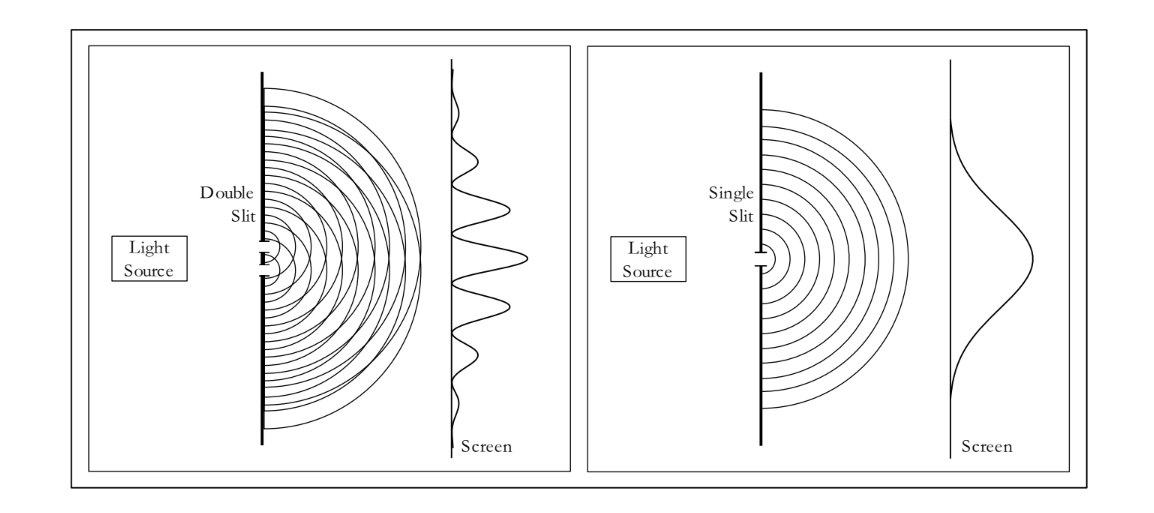
\includegraphics[width=1\linewidth]{../images/Doubleslit.png}
    \caption{Double slit and single-slit diffraction}
    \label{fig:slitexperiment}
\end{figure}

Next, we consider the situation for waves, for example water waves. A water wave doesn't go through either slit 1 or slit 2, it goes through both. you should imagine the rest of 1 water wave as it approaches the slit. As it hits the slit, the wave is blocked at all places but the two slits, and waves on the other side are generated at each slit as depicted in the figure \ref{fig:slitexperiment}.

When the new waves generated at each slit run into each other, interference occurs. We can see this by plotting the intensity (that is, the amount of energy carried by the waves) at each point y along the viewing screen. What we see is the familiar interference pattern seen in figure \ref{fig:slitexperiment}. The dark patches of the interference pattern seen in figure \ref{fig:slitexperiment} occur where the wave from the first slit arrives perfectly out of sync with wave from the second slit, while the bright points are where the two arrive in sync. For example, the bright spot right in the middle is bright because each wave travels the exact same distance from their respective slits to the screen, so they arrive in sync. The first dark spots are where the wave from one slit traveled exactly half of a wavelength longer than the other wave, thus they arrive at opposite points in their cycle and cancel. Here, it is not the intensities coming from each slit that add, but the height of the wave. This differs in the case of bullets: $I_{12}(y)\neq I_1(y)+I_2(y)$, but $h_{12}(y)=h_1(y)+h_2(y)$, and $I_{12}(y)=h(y)^2$, where $h9y)$ is the height of the wave and $I(y)$ is the intensity, or energy, of the wave.

Before we can say what light does, we need one more crucial piece of information. What happens when we turn down the intensity in both of these examples?

In the case of bullets, turning down the intensity means turning down the rate at which the bullets are fired. When we turn down the intensity, each time a bullet hits the screen it transfers the same amount of energy, but the frequency at which bullets hit the screen becomes less.

With water waves, turning down the intensity means making the wave amplitudes smaller. Each time a wave hits the screen it transfer less energy, but the frequency of the waves hitting the screen is unchanged.

Now what happens when we do this experiment with light. As Young observed in 1802, light makes an interference pattern on the screen. From this observation he concluded that the nature of light is wavelike, and reasonably so!.  However, Young was unable at the time to turn down the intensity of light to see the problem with the wave explanation.

Picture now that the observation screen is made of thousands of tiny little photo-detectors that can detect the energy they absorb. For high intensities the photo-detectors individually are picking up a lot of energy, and when we plot the intensity against the position y along the screen we see the same interference pattern as described earlier. Now, turn the intensity of the light very very low. At first, the intensity scales down lower and lower everywhere, just like a wave. But as soon as we get low enough, the energy that the photo-detectors report reaches a minimum energy, and all of the detectors are reporting the same energy, call it $E_0$, just at different rates. This energy corresponds to the energy carried by an individual photon, and at this stage we see what is called quantization of light. Photo-detectors that are in the bright spots of the interference pattern report the energy $E_0$ very frequently, while the darker areas report the energy $E_0$ at lower rates. Totally dark points still report nothing. This behavior is the behavior of bullets not waves! We now see that photons behave unlike either bullets or waves, but like something entirely different.

Turn down, the intensity so low that only one photo-detector reports something each second. in other words, the source only sends one photon at at time. Each time a detector receives a photon, we record where on the array it landed and plot it on a graph. The distribution we draw will reflect the probability that a single photon will land at a particular point.

Logically we think that the photon will either go through one slit or the other. Then, like the bullets, the probability that the photon lands at a point y should be $P_{12}(y)=P_1(y)+P_2(y)$ and the distribution we expect to see is the two peaked distribution of the bullets. But this is not what we see at all.

What we actually see is the same interference pattern as before! But how can this be? For there to be an interference pattern, light coming from one slit must interfere with light from the other slit; but there is only one photon going through at a time! The modern explanation is that the photon actually goes through both the slits at the same time, and interferes with itself. The mathematics is analogous to that in the case of water waves. We say that the probability $P(y)$ that a photon is detected at $y$ is proportional to the square of some quantity $a(y)$, which we call a probability amplitude. Now probability amplitudes for different alternatives add up. So $a_{12}(y)=a_{1}(y)+a_2(y)$. But $P_{12}(y)=|a_{12}(y)|^2\neq |a_1(y)|^2+|a_2(y)|^2=P_1(y)+P_2(y)$.

Logically, we can ask which slit the photon went through, and try to measure it. Thus, we might construct a double slit experiment where we put a photo-detector at each slit, so that each time a photon comes through the experiment we see which slit it went through and where it hits on the screen. but when such an experiment is performed, the interference pattern gets completely washed out! The very fact that we know which slit the photon goes through makes the interference pattern go away. This is the first example we see of how measuring a quantum system alters the system.

Here the photon looks both like a particle, a discreet package , and a wave that can have interference. It seems that the photon acts like both a wave and a particle, but at the same time it doesn't exactly behave like either. This is what is commonly known as the wave-particle duality, usually though of as a paradox. The resolutions is that the quantum mechanical behavior of matter is unique, something entirely new.

What may be more mind blowing still is that if we conduct the exact same experiment with electrons instead of light, we get the exact same results! Although it is common to imagine electrons as tiny little charged spheres, they are actually quantum entities, neither wave nor particle but understood by their wave function.

The truth is that there is no paradox, just an absence of intuition for quantum entities. Why should they be intuitive? Things on our scale do not behave like wave functions, and unless we conduct wild experiments like this we do not see the effects of quantum mechanics.

\section{Computation}
A computation corresponds to some input to a processor which then performs instructions may be using look-up tables(oracles)/libraries on input and produces an output. Similar is seen in the physical process in nature where for Physical processes in some initial state through some interactions goes to the final state. Note that not every physical process is a computation but for every computation there must be an underlying physical process. 


Mathematical description of what goes on in a computer needs physical hardware to implement the task. Whether certain abstract mathematical operations are possible or not ultimately depends on whether there exists some suitable physical hardware to implement it. Thus, potentialities and limitation of a computer depends on the available hardware.

At the fundamental level there are only four types of interactions: Strong and weak interactions do not play any role in our day to day devices. Gravity acts as a fixed background but does not impact much of our devices. Electromagnetism is the mostly used force in its various forms to control and manipulate the dynamics of our devices.
Tasks which can be performed on a computer are limited by the manner in which we can use various aspects of electromagnetic interactions.

\begin{figure}
    \centering
    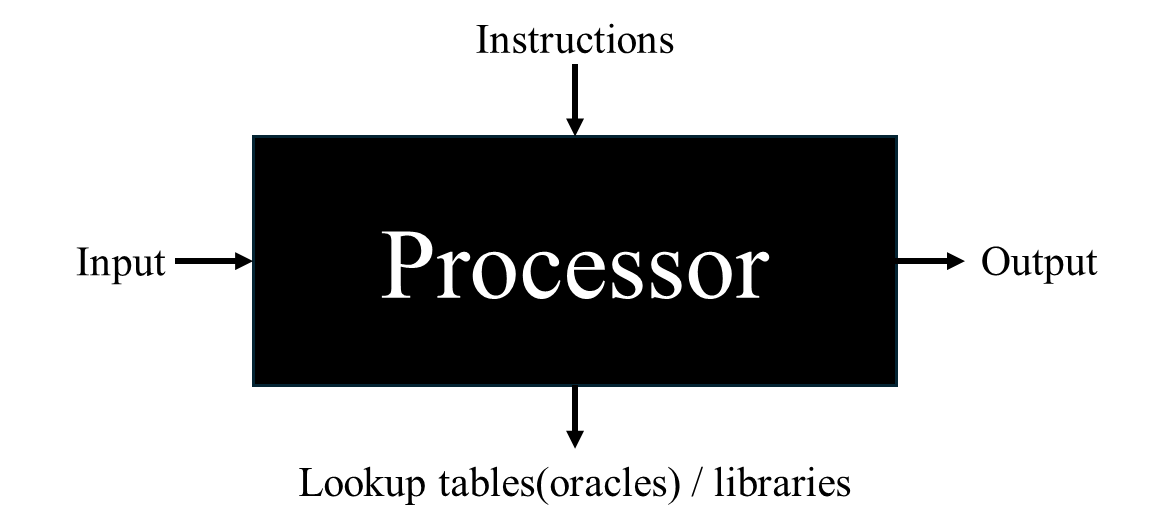
\includegraphics[width=0.75\linewidth]{../images/computation.png}
    \caption{Computation}
    \label{fig:computation}
\end{figure}

Computer is a device that purposefully processes meaningful information. From a philosophical point of view in order to understand a definition we need to keep on understanding the words in its definition till its intuition is rooted in our past experience of the physical world. Here, information means an abstract quantity by represented by some mathematical variables. Processes refers to the manipulation of physical states by a device. Meaningful relates to the mapping between the mathematical variables and physical state. Purposefully means contained in algorithmic design of instructions. For example, Boolean logic based computers have mathematical variables as $\{0,1\}$. Physical states are $\{off,on\}$ of transistors. Here 0 is mapped to off and 1 is mapped to on state. Algorithmic instructions manipulate the values 0 and 1.

It is a wonderful property of nature that physical properties and observations can be represented by abstract mathematical variables by designing a suitable map, and working on the variables without any reference to their physical origin and afterwards carrying out transformations insert physical meaning back. For example, a phone can be copied and then sent and then interpreted back as phone number. Thus, Physical data is converted into abstract mathematical information removing all its features of physical realisation which is then processed by rules of mathematics acting in terms of language and its grammar. Then its physical interpretation is practically useful knowledge. Note that data without is physical realisation is information and knowledge is processed information along with its physical interpretation. Thus, learnign mathematical concepts needs a support of their physical realisations in some or the other form.

Now we can define what we want a computer to do. We want a general information Processing system (which is limited by Physics). Note that there are some special purpose devices that do exist (like GPUs). They should have an efficient design meaning that they should be able to tackle as many different problems that are in same class i.e. all problems which can be expressed using the same mathematical language. Thus, there is a need for optimization. By optimization we mean using minimum physical resources in terms of time (to run as quickly as possible), space (to keep processor size/memory small), energy (to use less power) etc. required reducing some physical quantity. In terms of software: it is regarding the number of variables and instructions and memory used for running an algorithm. In terms of hardware, it is the physical implementation of how variables are mapped to physical components (component size, energy consumed, components neighbour).

Whenever we use ready made look-up tables called oracles we consider the number of times oracle is called for calculating the complexity.

There exists a hierarchy of operations connecting software and hardware. In a computer data is fed to pre-processors that converts the data to some mathematical representation (high level language) which then goes to compiler (converts instructions into low level assembly code). There is much smaller vocabulary at this level. Then, it gets converted to assembly code and then to machine code which then is seen as implementation and programmer level. All these are low level (Hardware) fixed whereas the data and pre-processing, compiler are high level (software) level and hence flexible. A living organism also shows a similar hierarchy where environment signal are picked up by sense and then brain interprets and takes actions. Here, in this case brain uses experience, takes initiative, figures out new ways. which are then send as electro-chemical signals to the nervous systems then to cells where cells take actions in the form of proteins, enzymes which is all encoded in our DNA. In computers at low level, it requires low level mapping where physical components (physical devices) must carry out both information and interpretation. 

We desire to minimise resources which in turn leads to increase in noise and fluctuations/errors as limited by the Second Law of Thermodynamics and thus increase in errors. Thus, there exists a tradeoff in between the resources and errors. Hence clarity is essential. Thus, the approach for solving this problem is fixing the level of allowed errors and then to minimise resources as much as possible. 



\section{The coin Experiment: Analogy for intuition}
Consider an unbiased coin, a preliminary high school knowledge will tell you that if you toss a coin the probability of getting heads or tails either is $1/2$. Given a coin we can either toss it or look at the coin. Note that we don't know the side of the coin facing up unless and until we look at the coin. This action of looking at the coin let us call it as measurement. Thus, given a coin we can perform two operations, either measurement or toss a coin i.e. we can either see the side facing up or toss the coin. Let us now move on to the mathematical framework. Consider that we don't know the state of the coin initially, so it can be either heads or tails with equal probability of $1/2$ and hence can be written as
\[
\begin{pmatrix} 1/2 \\ 1/2 \end{pmatrix}
\]
where the entry in the first row corresponds to the probability of seeing heads ($=1/2$) and the entry in the second row corresponds to seeing tails ($=1/2$) upon measurement. Note that the sum of the entries in the column must be equal to 1. Now we can either look at the coin i.e. do a measurement or toss a coin. Let us toss the coin. Now since it's an unbiased coin the state of the vector will not change even after tossing the coin. Mathematically, this can be represented by a linear operation i.e. matrix-vector multiplication operation where the matrix corresponds to the operation of tossing the coin. This is shown as follows:
\[
\begin{pmatrix} 1/2 & 1/2 \\ 1/2 & 1/2 \end{pmatrix} \begin{pmatrix} 1/2 \\ 1/2 \end{pmatrix} = \begin{pmatrix} 1/2 \\ 1/2 \end{pmatrix}
\]
where the matrix corresponds to the operation of tossing a coin and the vector is the state vector of the coin before tossing the coin. The state vector indicates that the probability of measuring heads is $1/2$ and probability measuring tails is $1/2$ upon measurement. Now if we perform a measurement i.e. look at the coin the probabilistic state of the coin it will either collapse to the following
\[
\begin{pmatrix} 1 \\ 0 \end{pmatrix} or \begin{pmatrix} 0 \\ 1 \end{pmatrix} 
\]
 for heads and tails respectively. Let us call this as basis states. Thus, if we perform another measurement the next time we will get Heads with certainty or tails with certainty depending upon the results of the previous measurement as indicated by the state vector which is also consistent with the real world results. Thus, we have a working mathematical framework of tossing a coin. Suppose, upon measurement we had found that the result of the state was head and hence the state vector was $\begin{pmatrix} 1 \\ 0 \end{pmatrix}$. Now when we toss the coin, we get
 \[
 \begin{pmatrix} 1/2 & 1/2 \\ 1/2 & 1/2 \end{pmatrix} \begin{pmatrix} 1 \\ 0 \end{pmatrix} = \begin{pmatrix} 1/2 \\ 1/2 \end{pmatrix}
 \]
 which is as we expected that now upon measurement the probability of getting heads is equal to the probability of getting tails $(=1/2)$. All the mathematical framework is consistent with the real world experiences. Now, no matter how many times we toss the coin the state of the vector will remain the same i.e. probability of getting heads is equal to the probability of getting tails $=1/2$ unless and until we perform a measurement by looking at the coin whereupon it collapses to one of the basis states.
Note that the state vector is also the eigen vector corresponding to the eigen value of 1 of the matrix (operation matrix of tossing the coin).

Let us make it more interesting by taking a biased coin. Let the probability of getting heads be 1/4 and of getting tails be 3/4. Thus the state vector corresponding to it will be
\[
\begin{pmatrix} 1/4 \\ 3/4 \end{pmatrix}
\]
We can now perform a measurement or toss the coin. Consider we don't know the state initially and we toss the coin, then the matrix-vector linear operation corresponding to the operation of tossing the coin and the state vector will be
\[
\begin{pmatrix} 1/4 & 1/4 \\ 3/4 & 3/4 \end{pmatrix}\begin{pmatrix} 1/4 \\ 3/4 \end{pmatrix} = \begin{pmatrix} 1/4 \\ 3/4 \end{pmatrix}
\]
Thus indicates that upon measurement we will get heads with a probability of $1/4$ and tails with a probability of $3/4$. No matter how many times we toss the coin the state of the vector will remain the same. Upon measurement the state will collapse to one of the basis states
\[
\begin{pmatrix} 1 \\ 0 \end{pmatrix} or \begin{pmatrix} 0 \\1 \end{pmatrix}
\]
Say upon measurement we found that it was Tails i.e. the state vector collapsed to $\begin{pmatrix} 0 \\1\end{pmatrix}$. Then again upon tossing the coin the state vector again be in a probabilistic state as follows:
\[
\begin{pmatrix} 1/4 & 1/4 \\3/4 & 3/4 \end{pmatrix} \begin{pmatrix} 0 \\ 1 \end{pmatrix} = \begin{pmatrix} 1/4 \\ 3/4\end{pmatrix}
\]
as expected. The state of the coin after tossing will again be a probabilistic state will the probability of getting heads being $1/4$ and the probability of tails being $3/4$ upon measurement.

Now, let us take this a step further. Note that we can write $\begin{pmatrix} 1/4 \\ 3/4 \end{pmatrix} = 1/4 \begin{pmatrix} 1 \\ 0 \end{pmatrix} + 3/4 \begin{pmatrix} 0 \\1\end{pmatrix}$. Note that we can write the state vector of the coin at any intermediate state as a linear combination of the basis state (since the basis states are tow linearly independent orthogonal vectors, they span the entire 2D Vector space and hence any vector in the 2D space can be written as a linear combination of these two vectors). Thus, we can write the state vector of coin at any time as the linear combination of the basis states as shown below:
\[
\begin{pmatrix} \alpha \\ \beta \end{pmatrix} = \alpha \begin{pmatrix} 1 \\ 0 \end{pmatrix} + \beta \begin{pmatrix} 0 \\ 1 \end{pmatrix}
\]
for $\alpha, \beta \in \mathbb{R}$. Thus, the state vector of the coin always exists as a linear combination of the basis states. The operation of tossing the coin is simply a matrix-vector multiplication with the state as follows.
\begin{align*}
\begin{pmatrix} 1/4 & 1/4 \\3/4 & 3/4 \end{pmatrix} \begin{pmatrix} \alpha \\ \beta \end{pmatrix} &= \alpha \begin{pmatrix} 1/4 & 1/4 \\3/4 & 3/4 \end{pmatrix} \begin{pmatrix} 1 \\ 0 \end{pmatrix} + \beta \begin{pmatrix} 1/4 & 1/4 \\3/4 & 3/4 \end{pmatrix} \begin{pmatrix} 0 \\ 1 \end{pmatrix}\\
&= \alpha \begin{pmatrix} 1/4 \\ 3/4 \end{pmatrix} + \beta \begin{pmatrix} 1/4 \\ 3/4 \end{pmatrix}\\
&=(\alpha + \beta) \begin{pmatrix} 1/4 \\ 3/4 \end{pmatrix}
\end{align*}
Note that if we perform a measurement just after another measurement then the state of the vector remains unchanged i.e. say upon measurement we saw that the state vector was Heads then if we perform another measurement operation just after the first one then the state vector will not change and will remain as Heads. No matter the amount of time you perform consecutive measurements the state vector once collapsed to either of the basis state in the first measurement remains the same throughout. But if we perform a matrix operation (coin toss) it will then again be in a probabilistic (or linear combination sometimes called a superposition) state.

In conclusion, we saw that the state vector is a linear combination of the basis vector (with real coefficients) and there are two categories of operations we can perform on the coin either measurement or toss a coin. Similar is the case with qubits. This linear combination of basis states is what sometimes referred to as the superposition principle.

For a qubit, the state vector is a linear combination (also called superposition) of the basis states (or vectors) (with complex coefficients) and there are two types of operations we can perform on qubits either measurement (in which case it collapses to one of the basis states) or a matrix multiplication (here the matrix is unitary as a result of Axiom of Quantum mechanics we will later see). Thus, we can define the basis vectors/states for the purpose of quantum computing as follows:
\[
\ket{0}=\begin{pmatrix} 1 \\ 0 \end{pmatrix}, \ket{1}=\begin{pmatrix} 0 \\ 1 \end{pmatrix}
\]
and thus the state vector of a qubit is given as
\[
\ket{v}=\begin{pmatrix} \alpha \\ \beta \end{pmatrix} = \alpha \begin{pmatrix} 1 \\ 0 \end{pmatrix} + \beta \begin{pmatrix} 0 \\ 1 \end{pmatrix}
\]
where $\alpha,\beta \in \mathbb{C}$. Thus, we can perform either of the two operations measurement or a matrix operation (manipulation of qubits). Upon measurement it will either collapse to either one of the basis states. The condition for manipulation of a matrix by a qubit is that it must be unitary. Thus, matrix multiplication will be as follows:
\[
Uv=\begin{pmatrix} a & b \\ c & d \end{pmatrix}\begin{pmatrix} \alpha \\ \beta \end{pmatrix} =\begin{pmatrix} a \alpha + b\beta \\ c\alpha + d\beta \end{pmatrix}
\]
where U is a unitary matrix ($U^{\dagger}U=UU^{\dagger}=I$).
There is another restriction that the norm of the state vector must be unit norm ($\|\ket{v}\|=1$). All these restrictions will be further explained in depth as part of axioms of Quantum Mechanics.

\section{Quantum Information}
We will look at Quantum information, a concept on which quantum computation is based.

\subsection{A probabilistic model}
Let us start classically, with a model that will probably seem completely simple to every one. Imagine that we have some physical device, called X, that has some finite, non-empty set $\Sigma$ of possible state (classical states). For example, we might have $\Sigma = \{0,1\}$, in which case we would think of X as representing a bit. For the following discussion let us restrict ourselves to this example (but keep in mind that everything can be generalized to sets other than $\{0,1\}$).

Suppose that we do not necessarily have complete information about the state of X, but instead represent our knowledge of its state by assigning probabilities to different states. For example, we might have
\[
Pr[\text{state of X is 0}]=1/4
\]
\[
Pr[\text{state of X is 1}]=3/4
\]
Mathematically we can represent this type of knowledge about the state X with a probability vector, which is a column vector whose entries are all non-negative real numbers that sum to 1. In the case at hand, the associated probability vector is
\[
v=\begin{pmatrix} 1/4 \\ 3/4 \end{pmatrix}
\]
The understanding is that the entries of $v$ are indexed by $\Sigma$, and when we write such a vector in the above form we are using the most natural way of ordering the elements of $\Sigma$.$1/4$ entry indexed by 0, $3/4$ entry indexed by 1.

We may write $v[0]$ and $v[1]$ to refer to the entries of $v$ when necessary.

What happens when you look at X? Of course you will not see a probability vector $v$. instead you will see some element of $\Sigma$. If our representation of the state of X by a probability vector $v$ is in some way meaningful, you may as well imagine that the state you saw was determined randomly according to the probabilities associated with various states. Notice that by looking at the sate of X you effectively change the description of your knowledge of its state. Continuing with the above example, if you look and see that the state is 0, the description of your knowledge changes from $v$ to a new probability vector $w$:
\[
v=\begin{pmatrix} 1/4 \\ 3/4 \end{pmatrix} \rightarrow w=\begin{pmatrix} 1 \\ 0 \end{pmatrix}
\]
You know that the state is 0, and the vector w represents this knowledge. If you saw the state was 1 instead of 0, the vector would become
\[
\begin{pmatrix} 0 \\ 1 \end{pmatrix}
\]
instead.

What sorts of operation can you imagine performing on X? There are not very many deterministic operations: you could initialize X to either 0 or 1, you could not perform a NOT operation to X, or you could do nothing to X (which can still be considered an operation even though it has no effect). You could also perform an operation involving randomness - for instance perform a NOT operation with probability $1/100$, and other wise do nothing. I claim that any physically meaningful operation can be represented by a matrix, with the effect of the operation being determined by the matrix-vector multiplication. For instance, these four matrices
\[
INIT_0 = \begin{pmatrix} 1 & 1 \\ 0 & 0\end{pmatrix}, INIT_1= \begin{pmatrix} 0 & 0 \\ 1 & 1 \end{pmatrix}, 
NOT = \begin{pmatrix} 0 & 1 \\ 1 & 0\end{pmatrix}, and \quad I = \begin{pmatrix} 1 & 0 \\ 0 & 1\end{pmatrix}
\]
represent the deterministic operators mentioned above. For example, if our knowledge of the state of X is represented by
\[
v=\begin{pmatrix}1/4 \\ 3/4 \end{pmatrix}
\]
and we perform a NOT operation on X, the new probability vector that results is
\[
w=\begin{pmatrix} 0 & 1 \\ 1 & 0 \end{pmatrix}\begin{pmatrix} 1/4 \\3/4 \end{pmatrix} =\begin{pmatrix}3/4 \ 1/4 \end{pmatrix}
\]
The probabilistic operation mentioned above is represented by the matrix
\[
\begin{pmatrix} \frac{99}{100} & \frac{1}{100} \\ \frac{1}{100} & \frac{99}{100} \end{pmatrix}
\]
All of these matrices have the property that (i) all entries are non-negative real numbers, and (ii) the entries of each column sum to 1. In other words, every column is a probability vector. Such matrices have a name: they are called stochastic matrices. in the simple model we are discussing, physically meaningful operations are described by stochastic matrices. it works the other way as well; any stochastic matrix describes some physically meaningful operation.

As mentioned before, this entire pictures is easily generalized to the case where $\Sigma$ is not necessarily $\{0,1\}$. In general the dimension of the vectors and matrices will be equal to the size of $\Sigma$.

\subsection{Quantum bits (qubits)}
The framework of quantum information works in a similar way to the simple probabilistic model we just saw, but with some key differences. Let us again imagine that we have a physical device called X. As before we imagine there is some set of $\Sigma$ of possible states of X, and we will again consider for now just the simple case $\Sigma=\{0,1\}$. At this point, to avoid confusion let us not refer to elements of $\Sigma$ as \textit{classical states}. Intuitively one can think of a classical state that you as a human can look at, touch and recognize without ambiguity. The device X will represent the quantum analogue of a bit, which we call a qubit.

We will represent out knowledge of X with column with column vectors indexed by $\Sigma$, but this time they will not be probability vectors. Instead of representing probability distributions, the vectors represent what we call a superposition or just a state (by which we mean a quantum state). For example, here are a few vectors representing superpositions:
\[
\begin{pmatrix} \frac{1}{\sqrt{2}} \\ -\frac{1}{\sqrt{2}} \end{pmatrix}, \begin{pmatrix} 1 \\ 0 \end{pmatrix}, \begin{pmatrix} \frac{3}{5} \\ \frac{4\iota}{5} \end{pmatrix}
\]

Notice that the entries in these vectors are not probabilities: they are not necessarily non-negative (in fact they are not even necessarily real numbers), and they do not necessarily sum to 1. We call these numbers amplitudes instead of probabilities. The condition that replaces probabilities summing to 1 in a probability vector is this: vectors representing superpositions have Eucledian length equal to 1. In the simple case at hand where $\Sigma = \{0,1\}$, this means that any vector representing a superposition has the form
\[
\begin{pmatrix} \alpha \\ \beta \end{pmatrix} 
\]
for $\alpha, \beta \in \mathbb{C}$ satisfying $|\alpha|^2+|\beta|^2=1$.

Similar to the probabilistic case, if you look at the qubit X you will not see a superposition. Instead you will see either 0 or 1 just like before. The probability associated with the two possible outcomes is given by the absolute value squared of the associated amplitude-so i the superposition of X is represented by the vector
\[
\begin{pmatrix} \alpha \\ \beta \end{pmatrix}
\]
any you look at X, you will see 0 with probability $|\alpha|^2$ and 1 with probability $|\beta|^2$. This is why we have the condition $|\alpha|^2+|\beta|^2$, because the probabilities have to sum to 1 for the model to make sense. The same rules apply as for the probabilities case for determining the superposition of X after you look at it: the superposition becomes
\[
\begin{pmatrix} 1 \\ 0 \end{pmatrix} or \begin{pmatrix} 0 \\1 \end{pmatrix}
\]
depending on whether you see 0 or 1, respectively.

So far the model does not seem qualitatively different from the probabilistic model, but that changes a lot when the possible operations that can be performed are considered. Again the possible operations are represented by matrices; but now instead of being stochastic matrices, the matrices that represent valid physical operations correspond to unitary matrices. A matrix is unitary if and only if it preserves the Eucledian norm. Fortunately there is a very simple condition to check this: a matrix U is unitary if and only if
\[
U^{\dagger}U=UU^{\dagger}=I
\]
where $U^{\dagger}$ is the conjugate transpose of U (meaning that you take the transpose of U and then take the complex conjugate of each of the entries). For example, these are unitary matrices:
\[
H=\begin{pmatrix} \frac{1}{\sqrt{2}} & \frac{1}{\sqrt{2}} \\ \frac{1}{\sqrt{2}} & -\frac{1}{\sqrt{2}} \end{pmatrix}, I=\begin{pmatrix} 1 & 0 \\0 & 1 \end{pmatrix}, NOT=\begin{pmatrix} 0 & 1 \\ 1 & 0\end{pmatrix}, R_{\theta} = \begin{pmatrix} \cos (\theta) & -\sin (\theta) \\ \sin(\theta) & \cos (\theta) \end{pmatrix}
\]
(for any real number $\theta$ in the case of $R_{\theta}$). For example, if X is a superposition described by
\[
v=\begin{pmatrix} 1 \\ 0 \end{pmatrix}
\]
and the operation corresponding to the matrix H (called the hadamard transform) is performed, the superposition becomes
\[
Hv=\begin{pmatrix} \frac{1}{\sqrt{2}} & \frac{1}{\sqrt{2}}\\\frac{1}{\sqrt{2}} & -\frac{1}{\sqrt{2}} \end{pmatrix}
\]
If you measured X at this point you would see outcome 0 or 1 with probability $1/2$. If you didn't measure and instead applied the Hadamard transform again, the superposition would become
\[
\begin{pmatrix} \frac{1}{\sqrt{2}} & \frac{1}{\sqrt{2}} \\ \frac{1}{\sqrt{2}} & -\frac{1}{\sqrt{2}} \end{pmatrix} = \begin{pmatrix} 1 \\ 0 \end{pmatrix}
\]
To recapitulate, these are the two things you can do to a qubit:
\begin{enumerate}
    \item \textbf{Perform a measurement.} If the superposition of the qubit is
    \[
    \begin{pmatrix} \alpha \\ \beta \end{pmatrix}
    \]
    and a measurement is performed, the outcomes is 0 or 1, with probabilities $|\alpha|^2$ and $|\beta|^2$, respectively. The superposition of the qubit becomes
    \[
    \begin{pmatrix} 1 \\ 0 \end{pmatrix}, \begin{pmatrix} 0 \\1 \end{pmatrix}
    \]
    depending on whether the measurement outcome was 0 or 1.
    \item \textbf{Perform a Unitary operation} For any unitary matrix U, the operation described by $U$ transforms any superposition $v$ into the superposition $Uv$.
\end{enumerate}

\begin{example}
    Suppose your friend has a qubit that he knows is in one of the two superpositions
    \[
    v_0=\begin{pmatrix} \frac{1}{\sqrt{2}} \\ \frac{1}{\sqrt{2}} \end{pmatrix} or v_1\begin{pmatrix} \frac{1}{\sqrt{2}} \\ -\frac{1}{\sqrt{2}} \end{pmatrix}
    \]
    but he isn't sure which. How can you help him determine which one it is?
    Measuring right away will not help - you would see a random bit 0 or 1 with equal probability in either case. instead,you should perform a Hadamard transform and them measure. Performing the hadamard transform changes the superposition as follows:
    \[
    Hv_0=\begin{pmatrix} 1 \\ 0\end{pmatrix} \quad and \quad Hv_1 =\begin{pmatrix} 0 \\1 \end{pmatrix}
    \]
    Now if you measure, you will see 0 (with certainty, meaning probability 1) if the original superposition was $v_0$ and you will see 1 (with certainty) if the original superposition was $v_1$.
\end{example}

Thus instead of being just 0 and 1, quantum bits can be in a superposition between 0 and 1. Since "quantum bit" is somewhat long, researchers simply use the term "qubit" to refer to a quantum bit. Thinking of bit as vectors, a qubit can be described by a vector $\ket{v} \in \mathbb{C}^2$. the vector space $\mathbb{C}^2$. The vector space $\mathbb{C}^2$ is also known as the state space of the qubit. An example of qubit state is
\[
\ket{+}=\frac{1}{\sqrt{2}}(\ket{0}+\ket{1})
\]
It turns out that in order to be a valid qubit, $\ket{v}$ must be normalized, just as the vectors $\ket{0}$ and $\ket{1}$ corresponding to classical bits were indeed normalized. For the moment, let us just take this as a rule leading to the following definition.

\begin{definition}
    \textbf{Qubit} A (pure) state of a qubit can be represented as a 2-dimensional ket vector $\ket{\psi} \in \mathbb{C}^2$.
    \[
    \ket{\psi}=\alpha\ket{0}+\beta\ket{1}, \quad \text{where $\alpha,\beta \in \mathbb{C}$ and $|\alpha|^2+|\beta|^2=1$}
    \]
    The condition on $\alpha$ and $\beta$ means that $\ket{\psi}$ is normalized. These complex numbers $\alpha$ and $\beta$ are also called amplitudes of $\ket{\psi}$.
\end{definition}

Throughout these lectures we will be mostly focusing on encoding information in qubits. However in general, quantum information can also be encoded in higher dimensional quantum systems. Therefore, one can similarly define a qudit as below:
\begin{definition}
    A qudit, or a d-dimensional quantum system can be represented as a d-dimensional ket vector $\ket{\psi} \in \mathbb{C}^d$
    \[
    \ket{\psi}=\sum_{i=0}^{d-1} \alpha_i\ket{i}, \quad \text{where $\forall i, \alpha_i \in \mathbb{C}$ and $\sum_{i=0}^{d-1} |\alpha_i|^2=1$ }
    \]
    The condition on the coefficients $\alpha_i$ means that $\ket{\psi}$ is a vector of length of 1.
\end{definition}
\begin{example}
    An example of a qubit is given by the vector $\ket{-}=\frac{1}{\sqrt{2}}(\ket{0}-\ket{1})$. The length of $\ket{-}$ is
    \[
    \braket{-|-}=\sqrt{\frac{1}{2}\begin{pmatrix} 1 & -1 \end{pmatrix} \begin{pmatrix} 1 \\ -1 \end{pmatrix}}=\sqrt{\frac{1}{2}2}=1
    \]
    So $\ket{-}$ is normalized.
\end{example}
\begin{example}
    Verify that for all values of $\theta$, $\ket{\psi}=\cos (\theta) \ket{0} + \sin (\theta) \ket{1}$ is a valid qubit state.
    \[
    |\cos (\theta)|^2+|\sin (\theta)|^2=\cos^2 (\theta) + \sin^2 (\theta)=1
    \]
    Thus, clearly it is normalized for all values of $\theta$.
\end{example}
In our definition of qubits, we started from a way to write classical bits as vectors $\ket{0}$ and $\ket{1}$. Note that these two vectors are orthonormal, which in the quantum notation can be expressed as $\braket{1|0}=0$ and $\braket{1|1}=\braket{0|0}=1$. These two vectors thus form a basis for $\mathbb{C}^2$, in that any vector $\ket{v}\in \mathbb{C}^2$ can be written as $\ket{v}=\alpha \ket{0} +\beta \ket{1}$ for some coefficients $\alpha,\beta \in \mathbb{C}$. This basis corresponding to "classical" bits is used so often that it carries a special name:

\begin{enumerate}
    \item \begin{definition}
        \textbf{Computational Basis/Standard Basis:} Consider the 2-dimensional complex vector space $\mathbb{C}^2$. The standard basis, or sometimes known as the computational basis, $\mathcal{S}=\{\ket{0},\ket{1}\}$ is an orthonormal basis for this vector space, where the basis vectors are
        \[
        \ket{0}=\begin{pmatrix} 1 \\ 0 \end{pmatrix}, \ket{1}=\begin{pmatrix} 0 \\ 1 \end{pmatrix}
        \]
        In general, for a d-dimensional complex vector space $\mathbb{C}^d$. The standard basis or computational basis states are represented as $\ket{0},\ket{1},\ldots,\ket{d-1}$ where
        \[
        \ket{i}=\begin{pmatrix} \vdots \\ 0 \\ 1 \\ 0 \\ \vdots \\ \end{pmatrix}
        \]
        where it is a column vector of size $2^d \times 1$ with 1 at the ith location and 0 elsewhere.
    \end{definition}
Of course, there might be many other bases for $\mathbb{C}^2$. But here,we will discuss only those basis which are most frequently used.
    \item \begin{definition}\textbf{Hadamard Basis:} The Hadamard basis is an orthonormal basis in which the states are represented as $\mathcal{H}=\ket{+},\ket{-}$ where 
    \[\ket{+}=\dfrac{\ket{0}+\ket{1}}{\sqrt{2}}=\frac{1}{\sqrt{2}}\begin{pmatrix} 1 \\ 1 \end{pmatrix} \quad \text{and} \quad \ket{-}=\dfrac{\ket{0}-\ket{1}}{\sqrt{2}}=\frac{1}{\sqrt{2}}\begin{pmatrix} 1 \\-1\end{pmatrix}.
    \]
    \end{definition}
    \item \textbf{Y Basis:} The basis in which the states are represented as $\ket{+i},\ket{-i}$ where 
    \[\ket{+i}=\dfrac{\ket{0}+\iota\ket{1}}{\sqrt{2}}=\frac{1}{\sqrt{2}}\begin{pmatrix} 1 \\ \iota \end{pmatrix} \quad \text{and} \quad \ket{-i}=\dfrac{\ket{0}-\iota\ket{1}}{\sqrt{2}}=\frac{1}{\sqrt{2}}\begin{pmatrix} 1 \\ -\iota \end{pmatrix}
    \]
\end{enumerate}

\begin{example}
    We now verify that the hadamard basis is indeed orthonormal using the bra-ket notation as shown below:
    \[
    \braket{+|+}=\frac{1}{2} \begin{pmatrix} 1 & 1 \end{pmatrix} \begin{pmatrix} 1 \\ 1 \end{pmatrix} =\frac{1}{2}2=1\implies \sqrt{\braket{+|+}}=1
    \]
    So $\ket{+}$ is normalized. Furthermore, the inner product
    \[
    braket{+|-}=\frac{1}{2}\begin{pmatrix} 1 & 1 \end{pmatrix} \begin{pmatrix} 1 \\ -1 \end{pmatrix} = 0
    \]
    So $\ket{+}$ and $\ket{-}$ are orthogonal to each other.
\end{example}

\begin{example}
    Express $\ket{1}$ in the Hadamard basis. That is, find coefficients $\alpha$ and $\beta$ such that $\ket{1}=\alpha\ket{+}+\beta\ket{-}$.
    Clearly, putting $alpha=\frac{1}{\sqrt{2}}$ and $\beta=\frac{1}{\sqrt{2}}$ satisfies the system of linear equations.
\end{example}

The linear superposition $\ket{\psi}=\alpha\ket{0}+\beta \ket{1}$ is part of the private world of electron. For us to know the electron's state, we must make a measurement. making a measurement gives us a single classical bit of information 0 or 1. The simplest measurement is in the standard basis, and measuring $\ket{\psi}$ in this $\{\ket{0},\ket{1}\}$ basis yields 0 with probability $|\alpha|^2$, and 1 with probability $|\beta|^2$,.

One important aspect of the measurement process is that it alters the state of the qubit: the effect of the measurement is that the new state is exactly the outcome of the measurement. i.e., if the outcome of the measurement of $\ket{\psi}=\alpha \ket{0}+\beta\ket{1}$ yields 0, then following the measurement, the qubit is in the state $\ket{0}$. This implies that you cannot collect any additional information about $\alpha,\beta$ by repeating the measurement.

More generally, we may choose any orthogonal basis $\{\ket{v},\ket{w}\}$ and measure the qubit in that basis. To do this, we rewrite our state in that basis: $\ket{\psi}=\alpha'\ket{v}+\beta'\ket{w}$. The outcome is $v$ with probability $|\alpha'|^2$, and $\ket{w}$ with probability $|\beta'|^2$. If the outcome of the measurement on $\ket{\psi}$ yields $\ket{v}$, then as before, the qubit is then in state $\ket{v}$.

\subsection{Example of Qubits}
\subsubsection{Atomic Orbitals}
The electrons within an atom exist in quantized energy levels. Qualitatively these electronic orbits (or "orbitals" as we like to call them) can be thought of as resonating standing waves, in close analogy to the vibrating waves one observes on a tightly held piece of string. Two such levels can be isolated to configure the basis states for a qubit.

\subsubsection{Photon Polarization}
Classically, a photon may be described as a travelling electromagnetic wave. This description can be fleshed out using Maxwell's equation, but for out purposes we will focus simply on the fact that an electromagnetic wave has a polarization which describes the orientation of the electric field oscillations (see figure). So, for a given direction of photon motion, the photon's polarization axis might lie anywhere in a 2-d plane perpendicular to that motion. It is thus natural to pick an orthonormal 2-d basis (such as $\vec{x}$ and $\vec{y}$, or "vertical" and "horizontal") to describe the polarization state (i.e. polarization direction) of a photon. In a quantum mechanical description, this 2-d nature of the photon polarization is represented by a qubit, where the amplitude of the overall polarization state in each basis vector is just the projection of the polarization in that direction.

The polarization of a photon can be measured by using a polaroid film or a calcite crystal. A suitably oriented sheet transmits x-polarized photons and absorbs y-polarized photons. Thus a photon that is in a superposition $\ket{\phi}=\alpha\ket{x}+\beta \ket{y}$ is transmitted with probability $|\alpha|^2$. If the photon now encounters another polaroid sheet with the same orientation, then it is transmitted with probability 1. On the other hand, if the second polaroid sheet has its axes crossed at right angles to the first one, then if the photon is transmitted by the first polaroid, then it is definitely absorbed by the second sheet. This pair of polarized sheets at right angles thus blocks all the light. A somewhat counter-intuitive result is not obtained by interposing a third polaroid sheet at a 45 degree angle between the first two. Now a photon that is transmitted by the first sheet makes it through the next two with some non zero probability.

To see this first observe that any photon transmitted through the first filter is in the state, $\ket{0}$. The probability this photon is transmitted through the second filter is $1/2$ since it is exactly the probability that a qubit in the state $\ket{0}$ ends up in the state $\ket{+}$ when measured in the $\ket{+},\ket{-}$ basis. We can repeat this reasoning for the third filer, except now we have a qubit in state $\ket{+}$ being measured in the $\ket{0},\ket{1}$ basis - the change that the outcome is $\ket{0}$ is once again $1/2$.

\subsubsection{Spins}
Like photon polarization, the spin of a (spin-1/2) particle is a two-state system, and can be described by a qubit.Very roughly speaking, the spin is a quantum description of the magnetic moemnt of an electron which behaves like a spinning charge. The two allowed states can roughly be thought of as clockwise rotations ("spin-up") and counter clockwise rotations ("spin-down").

\subsection{Multiple Qubits}
In order to talk about what happens when we have multiple qubits, it will be helpful to briefly return to the probabilistic model from before. Suppose that X and Y are devices that implement bits. Then there are 4 possible states of the pair (X,Y), namely 00, 01, 10 and 11. Thus, our set of states $\Sigma$ corresponding to this pair is now $\{00,01,10,11\}$. In the probabilistic model we represent our knowledge of the state of the pair (X,Y) with a 4 dimensional probability vector. For example we could have the following probability vector
\[
\begin{pmatrix} \frac{1}{8} \\ \frac{1}{2} \\ 0 \\ \frac{3}{8} \end{pmatrix}
\]
with the first entry indicating the probability associated with state 00, second entry denoting the probability associated with state 01, third entry denoting the probability associated with state 10, fourth entry denoting the probability associated with state 11. (The vector indices are labelled by the states in the order given by binary notation.) Operations again correspond to stochastic matrices, but this time the matrices are $4 \times 4$ matrices. For example, the matrix
\[
\begin{pmatrix} 1 & 0 & 0 & 0 \\ 0 & 1 & 0 & 0 \\ 0 & 0 & \frac{1}{2} & \frac{1}{2} \\ 0 & 0 & \frac{1}{2} & \frac{1}{2} \end{pmatrix}
\]
is stochastic. It happens to correspond to the operation where you do nothing if the first bit is 0 but if the first bit is 1 then replace the second bit with a random bit.

The quantum variant works in an analogous way. If we have two qubits (X,Y), then a superposition of these two qubits is a 4-dimensional vector with Eucledian length equal to 1. For example:
\[
\begin{pmatrix} \frac{1}{\sqrt{2}} \\ 0 \\ \frac{\iota}{2} \\ -\frac{1}{2} \end{pmatrix}
\]
Measurement works the same way as before, except that the outcome will be two bits. For example, measuring the previous superposition gives results as follows:
\[
\text{00 with probability} |\frac{1}{\sqrt{2}}|^2=\frac{1}{2}
\]
\[
\text{01 with probability} |0|^2=0
\]
\[
\text{10 with probability} |\frac{\iota}{\sqrt{2}}|^2=\frac{1}{4}
\]
\[
\text{11 with probability} |=\frac{1}{2}|^2=\frac{1}{4}
\]
We can also measure only one qubit out of the two bits leaving the other alone, which is called partial measurement. We will later on see what happens in case of partial measurement. Unitary operations also work the same way as before, but this time are $4 \times 4$ matrices. For example, there is a 2 qubit unitary operation called controlled-NOT:
\[
\begin{pmatrix} 1 & 0 & 0 & 0 \\ 0 & 1 & 0 & 0 \\ 0 & 0 & 0 & 1\\ 0 & 0 & 1 & 0 \end{pmatrix}
\]
The same pattern is used for 3 qubits, 4 qubits etc. The dimension of the vectors and matrices grows exponentially: 8 dimensional vectors for 3 qubits, 16 dimensional vectors for 4 qubits, etc.

By the way there is no reason you cannot consider the model for any other choice of $\Sigma$, instead of $\Sigma$ corresponding to all possible strings of a given length. Typically, however, we will focus on the case where $\Sigma=\{0,1\}^n$ for positive integer n.

Classically, if we have two bits, we write them as '00','01',10','11'. But how can we write two qubits? One strategy is to again associate each of them two classical bits $x_1,x_2 \in \{0,1\}^2$ with a vector. labelling the first qubit A and the second one B, we could perform the mapping from strings to orthonormal vectors as
\[
0_A0_B\rightarrow \ket{00}_{AB}=\begin{pmatrix} 1 \\0 \\0 \\ 0 \end{pmatrix} \quad 0_A1_B\rightarrow \ket{01}_{AB}=\begin{pmatrix} 0 \\ 1 \\ 0 \\ 0 \end{pmatrix}
\]
\[
1_A0_B\rightarrow \ket{10}_{AB}=\begin{pmatrix} 0 \\ 0 \\ 1 \\0 \end{pmatrix} \quad 1_A1_B\rightarrow \ket{11}_{AB}=\begin{pmatrix} 0 \\ 0 \\ 0 \\ 1 \end{pmatrix}
\]
Note that the resulting vectors are in $\mathbb{C}^4$ with dimension $d=2^2=4$, where the dimension corresponds to the number of possible strings. It turns out that one can write a two-qubit state $\ket{\psi}_{AB}\in\mathbb{C}^4$ as a superposition of these vectors, where we again demand that $\ket{\psi}_{AB}$ is normalized. As an example, let us consider a state $\ket{\psi}_{AB}$ that is an equal superposition fo all above standard basis vectors:
\begin{align*}
\ket{\psi}_{AB}&=\frac{1}{2}\ket{00}_{AB}+\frac{1}{2}\ket{01}_{AB}+\frac{1}{2}\ket{10}_{AB}+\frac{1}{2}\ket{11}_{AB}\\
&=\frac{1}{2}\begin{pmatrix} 1 \\ 0 \\ 0 \\ 0 \end{pmatrix}+\frac{1}{2}\begin{pmatrix} 0 \\ 1 \\ 0 \\ 0 \end{pmatrix} + \frac{1}{2}\begin{pmatrix} 0 \\ 0 \\ 1 \\ 0 \end{pmatrix} + \frac{1}{2}\begin{pmatrix} 0 \\ 0 \\ 0 \\ 1 \end{pmatrix}\\
&=\frac{1}{2}\begin{pmatrix} 1 \\ 1 \\ 1 \\ 1 \end{pmatrix}
\end{align*}
The sum of amplitudes $\frac{1}{2}$ squared is $4\frac{1}{2^2}=1$, therefore $\ket{\psi}$ is a valid two qubit quantum state. As you might have guessed, we now proceed analogously when considering n qubits. To address
multiple qubits, we first look at the vector representation for multiple classical bits. For binary
strings of length $n$, consider the vector space $\mathbb{C}^n$, where each coordinate is labelled by a string
$x = x_1,..., x_n$. There are a total of $d = 2^n$ such strings, so we can label each string $x$ with a different
integer $i \in [1,d]$. We can then express the string $x$ as a vector $\ket{x_i}$ that is $0$ everywhere, except at the position labelled by $i$. A quantum state of $n$ qubits can then be written as
\[
\ket{\psi}=\sum_{x\in\{0,1\}^n} \alpha_x\ket{x}
\]
with $\alpha_x\in\mathbb{C}$ and $\sum_x |\alpha_x|^2=1$. The numbers $\alpha_x$ are again called amplitudes. We emphasize that the dimension of the vector space $\mathbb{C}^{2^n}$ increases exponentially with the number $n$ of bits. The space $\mathbb{C}^d$ with $d=2^n$ is thereby called the state space of n qubits. This means that we need an exponential number of parameters $\alpha_x$ to keep track of only n qubits, in sharp contrast to the $n$ parameters $x_1,\ldots , x_n$ to describe $n$ classical bits. You might wonder whether this was the only way to write down qubits. After all, we had simply chosen some mapping from strings of length $n$ to vectors in $\mathbb{C}^d$. Could we have chosen any other mapping from strings to vectors? It turns out that the answer to this is yes - as long as each string gets mapped to a vector that is orthonormal to the others. The mapping above, however, is very convenient and generally adopted within the realm of quantum computing. Analogous
to the case of a single qubit, the basis given by the set of vectors ${\ket{x} | x \in \{0,1\}^n}$ is called the
\textit{standard/computational basis}.

\begin{definition}
    \textbf{Standard basis for n qubits}. Consider the state space of n qubits $\mathbb{C}^d$. where $d=2^n$. For each distinct string $x \in \{0,1\}^n$. associate $x$ with a distinct integer $i \in \{1,2,\ldots ,d\}$. The standard basis for $\mathbb{C}^d$ is an orthonormal basis given by $\mathcal{S}_n=\{\ket{x} | x \in \{0,1\}^n$
    where $\ket{x}$ are d-dimensional vectors.
    \[
    \ket{x}=\begin{pmatrix} 0 \\ \vdots \\  1 \\ \vdots \\ 0 \end{pmatrix}
    \]
    where 1 is at the ith position.
\end{definition}
Let us summarize our discussion in the following definition of an n qubit quantum state.
\begin{definition}
    An n-qubit state $\ket{\psi} \in \mathbb{C}^d$ with $d=2^n$ can be written as a superposition of standard basis elements.
    \[
    \ket{\psi} = \sum_{x\in\{0,1\}^n}\alpha_x\ket{x}, \quad \text{where $\forall x, \alpha_x \in \mathbb{C}$ and $\sum_{x \in \{0,1\}^n} |\alpha_x|^2=1$}
    \]
\end{definition}
Let us now consider two examples of two qubit states. The first is so famous it carries a special
name and we will see it very frequently in the course of these notes.
\begin{example}
    Example 0.2.2 Consider two qubits A and B, in the two qubit state known as the EPR (Einstein, Podolsky and Rosen) pair, one can label the join state as AB
    \[
    \ket{EPR}_{AB}=\frac{1}{\sqrt{2}}(\ket{00}_{AB}+\ket{11}_{AB})=\frac{1}{\sqrt{2}}\begin{pmatrix} 1 \\ 0 \\ 0 \\ 0 \end{pmatrix} + \frac{1}{2}\begin{pmatrix} 0 \\ 0 \\ 0 \\ 1 \end{pmatrix}=\frac{1}{\sqrt{2}}\begin{pmatrix} 1 \\ 0 \\ 0 \\ 1 \end{pmatrix}
    \]
    which is an equal superposition between the vectors $\ket{00}_{AB}$ and $\ket{11}$. The length of this vector is given by the (square root o) inner product
    \begin{align*}
    \braket{EPR|EPR}_{AB}&=\frac{1}{\sqrt{2}}(\bra{00}_{AB}+\bra{11}_{AB})\cdot \frac{1}{\sqrt{2}}(\ket{00}_{AB}+\ket{11}_{AB})\\
    &=\frac{1}{2}(\braket{00|00}_{AB}+\braket{00|11}_{AB}+\braket{11|00}_{AB}+\braket{11|11}_{AB})\\
    &=\frac{1}{2}\cdot 2=1 \implies \sqrt{\braket{EPR|EPR}}=1
    \end{align*}
\end{example}
\begin{example}
    Consider the two qubit state
    \[
    \ket{\psi}_{AB}=\frac{1}{\sqrt{2}}(\ket{01}_{AB}+\ket{11}_{AB}\frac{1}{\sqrt{2}}\begin{pmatrix} 1\\ 0 \\ 0 \\ 1 \end{pmatrix}
    \]
    For this state, the second qubit always corresponds to bit 1. We will later see that this is significantly different state compared to $\ket{EPR}_{AB}$. It is not entangled!!.
\end{example}

\subsubsection{Tensor Products: How to combine qubits}

Returning again briefly to the probabilistic model, let us suppose that as before X and Y are devices
implementing bits, and the two devices are completely uncorrelated with one another—let us say
that the probability vector corresponding to X is
\[
v=\begin{pmatrix} \frac{2}{3} \\ \frac{1}{3} \end{pmatrix}
\]
and the probability vector corresponding to Y is
\[
w=\begin{pmatrix} \frac{1}{4} \\ \frac{3}{4} \end{pmatrix}
\]
Then the 4 dimensional probability vector corresponding to the pair (X, Y) is easily determined by
multiplying the corresponding probabilities. In particular, the resulting vector is
\[
v\otimes w= \begin{pmatrix} \frac{1}{6} \\ \frac{1}{2} \\ \frac{1}{12} \\ \frac{1}{4} \end{pmatrix}
\]
The operation $\otimes$ is called the Kronecker product or the tensor product. (It is most common in
quantum computing to use the term tensor product to refer to this operation.) In general, for any
two matrices
\[
A=\begin{pmatrix} a_{11} & a_{12} &\ldots & a_{1m} \\ a_{21} & a_{22} &\ldots &a_{2m} \\ \vdots & \vdots &\ddots & \vdots \\ a_{n1} & a_{n2} &\ldots & a_{nm} \end{pmatrix} \quad \text{and} \quad B=\begin{pmatrix} b_{11} & b_{12} &\ldots & b_{1l} \\ b_{21}& b_{22} & \ldots & b_{2l} \\ \vdots & \vdots & \ddots & \vdots \\ b_{k1} & b_{k2} & \ldots & b_{kl} \end{pmatrix}
\]
we define $A\otimes B$ to be the $nk \times ml$ matrix
\[
A\otimes B=\begin{pmatrix} a_{11}B & a_{12}B &\ldots & a_{1m}B \\ a_{21}B & a_{22}B &\ldots &a_{2m}B \\ \vdots & \vdots &\ddots & \vdots \\ a_{n1} B& a_{n2}B &\ldots & a_{nm}B \end{pmatrix}
\]
The definition works for vectors by thinking of them as matrices with only one column.
The tensor product satisfies many nice properties. For example, it is an associative operation;
$$(A \otimes B) \otimes  C = A \otimes (B \otimes C)$$ for any choice of matrices A, B and C. Thus, it makes sense to talk about products such as $A \otimes B \otimes C \otimes \ldots \otimes Z$ without including parentheses, because it doesn’t matter in which order the products are evaluated. Next, we have
\[
(A\otimes B)(C\otimes D)=(AC)\otimes (BD)
\]
for any choice of matrices A, B, C and D (assuming the sizes of the matrices are such that the
products AC and BD make sense). The distributive law holds for tensor products;
\[
A\otimes (B+C)=A\otimes B+A\otimes C \quad \text{and} \quad (A+B)\otimes C=A\otimes C+B\otimes C
\]
Also, for matrices A and B and any scalar $\alpha$, we have
\[
(\alpha A)\otimes B=A \otimes (\alpha B)=\alpha(A\otimes B)
\]
In other words, scalars “float freely” through the tensor product. A word of warning, however, is
that the tensor product is not commutative; in general it may be the case that $A\otimes B\neq B\otimes A$.

Not every probability vector v representing a distribution of (X, Y) can be written as a tensor
product. For example,
\[
v=\begin{pmatrix}1/2\\0\\0 \\ 1/2 \end{pmatrix}
\]
cannot be written as a tensor product. In this distribution we have
\[
Pr[\text{state of $(X,Y)$ is $00$}]=Pr[\text{state of $(X,Y)$ is }11]=\frac{1}{2}
\]
We say that X and Y are correlated in this case. The only way a probability vector can be written
as a tensor product is when the associated systems are uncorrelated (or independent).
As you might have guessed, we do exactly the same thing in the quantum case as in the classical, probabilistic case. If X and Y are qubits having associated superpositions
\[
v=\begin{pmatrix} \alpha \\ \beta \end{pmatrix} \quad \text{and} \quad w=\begin{pmatrix} \gamma \\ \delta \end{pmatrix}
\]
then the superposition of the pair (X, Y) is
\[
v\otimes w=\begin{pmatrix} \alpha\gamma \\ \alpha\delta \\ \beta\gamma\\\beta\delta \end{pmatrix}
\]
The superposition
\[
\begin{pmatrix} \frac{1}{\sqrt{2}} \\ 0 \\ 0 \\ \frac{1}{\sqrt{2}} \end{pmatrix}
\]
is an example of a superposition that cannot be written as a tensor product. In the quantum case,
this type of correlation between X and Y is special and we call it entanglement. We will talk about
entanglement a lot during the course.

For example, $\ket{1010}$ is a 16 dimensional vector with a 1 in the position indexed by $1010$ in binary (which is the eleventh entry because we start with 0000). The vector
\[
\frac{1}{\sqrt{2}} \ket{000000} +\frac{1}{\sqrt{2}}\ket{111111}
\]
would be written
\[
\begin{pmatrix} \frac{1}{\sqrt{2}} \\ 0 \\ \vdots \\ 0 \\\frac{1}{\sqrt{2}} \end{pmatrix}
\]
in the usual vector notation. An arbitrary vector with entries indexed by $\{0,1\}^n$, which perhaps refers to a superposition of n qubits, can again be written as a linear combination of the elements in the basis
\[
\{\ket{x}:x \in \{0,1\}^n\}
\]
for instance as
\[
\ket{\phi}=\sum_{x\in\{0,1\}^n} \alpha_x \ket{x}
\]

\begin{example}
    Let us suppose that we have two qubits X and Y in the superposition
    \[
    \begin{pmatrix} \frac{1}{\sqrt{2}} \\ 0 \\ 0 \\ \frac{1}{\sqrt{2}} \end{pmatrix}
    \]
    Using the Dirac notation we write this superposition as
    \[
    \frac{1}{\sqrt{2}}\ket{00}+\frac{1}{\sqrt{2}}\ket{11}
    \]
\end{example}

For every ket $\ket{\psi}$ there is a corresponding object $\bra{\psi}$, called a “bra”. You may think that this is
a strange name for a mathematical object, but the names “bra” and “ket” are derived from the the fact that when you put a bra and a ket together, you get a “bracket”. For this to make sense you
need to know what a bra is—for any vector $\ket{\psi}$ we define
\[
\bra{\psi}=(\ket{\psi})^{\dagger}
\]
which is the conjugate transpose of $\ket{\psi}$. In other words, $\bra{\psi}$ is the row vector you get by transposing
$\ket{\psi}$ and taking the conjugate of each of its entries. For instance:
\[
\ket{\psi}=\begin{pmatrix} \frac{1 + \iota }{2} \\ \frac{1}{\sqrt{2}} \end{pmatrix} \implies \bra{\psi}=\begin{pmatrix} \frac{1-\iota}{2} & \frac{1}{\sqrt{2}} \end{pmatrix}
\]
Now, when you juxtapose a bra and a ket, the implicit operation is matrix multiplication (thinking
of the vectors as matrices with only one row or one column). A row vector times a column vector
results in a scalar, and this scalar will be the inner product (or bracket) of the vectors involved. For
instance, if
\[
\ket{\psi}=\begin{pmatrix} \alpha \\ \beta \end{pmatrix} \quad \text{and}\quad \ket{\phi}=\begin{pmatrix} \gamma \\ \delta \end{pmatrix}
\]
then
\[
\braket{\psi|\phi} = \bra{\psi} \ket{\phi}=\begin{pmatrix} \overline{\alpha} & \overline{\beta} \end{pmatrix} \begin{pmatrix} \gamma \\ \delta \end{pmatrix} =\overline{\alpha}\gamma + \overline{\beta}\delta 
\]
When you have an expression such as
\[
\ket{\psi}=\sum_{x\in\{0,1\}^n} \alpha_x \ket{x}
\]
It is easy to express $\bra{\psi}$ using similar notation; it is
\[
\bra{\psi}=\sum_{x\in\{0,1\}^n} \overline{\alpha_x} \ket{x}
\]
When you juxtapose a ket and a bra in the opposite order, such as
\[
\ket{\psi}\bra{\phi}
\]
you do not get a scalar—a column vector times a row vector gives you a matrix. It is easy to
determine the action of this matrix on another vector. For instance,
\[
\ket{\psi}\bra{\phi}\ket{\gamma}=\ket{\psi}\braket{\phi|\gamma}=\braket{\phi|\gamma}\ket{\psi}
\]
Later on when we wish to speak at a higher level of abstraction about computational problems,
algorithms, etc., we may refer to |xi where x is some arbitrary mathematical object (such as a
matrix, a graph, or a list of numbers). In this case the interpretation is that we are implicitly
referring to the encoding of x with respect to some agreed upon encoding scheme.


Let’s imagine that we have two qubits, A and B. We know that we can describe the state of A
as $\ket{\psi}_A$and the one of B as $\ket{\phi}_B$. How can we write down the combined state $\ket{\psi}_{AB}$ of A and B together? The rule for computing the joint state is given by the so-called tensor product (sometimes also called Kronecker product). For two qubits
\[
\ket{\psi}_A=\alpha_A\ket{0}_A+\beta_A\ket{1}_A=\begin{pmatrix} \alpha_A \\ \beta_A \end{pmatrix}
\]
\[
\ket{\phi}_B=\alpha_B\ket{0}_B+\beta_B\ket{1}_B = \begin{pmatrix} \alpha_B \\ \beta_B\end{pmatrix}
\]
the joint state $\ket{\psi}_{AB} \in \mathbb{C}^2 \otimes \mathbb{C}^2$ can be expressed as the tensor product of individual vectors $\ket{\psi}_A$ and $\ket{\phi}_B$
\[
\ket{\psi}_{AB}=\ket{\psi}_A \otimes \ket{\phi}_B = \begin{pmatrix} \alpha_A \\ \beta_A \end{pmatrix} \otimes \ket{\psi}_B = \begin{pmatrix} \alpha_A \ket{\psi}_B \\ \beta_A\ket{\psi}_B \end{pmatrix} = \begin{pmatrix} \alpha_A \alpha_B \\ \alpha_A\beta_B \\ \beta_A\alpha_B\\ \beta_A\beta_B \end{pmatrix}
\]
As you may have guessed, we can of course also combine the state of two quantum systems A and
B if they are larger than just one qubit. The general definition of the tensor product of two vectors is given by
\begin{definition}
    Given two vectors $\ket{\psi_1} \in \mathbb{C}^{d_1}$ and $\ket{\psi_2}\in\mathbb{C}^{d_2}$ respectively, the tensor product is given by
    \[
    \ket{\psi_1}\otimes \ket{\psi_2}  = \begin{pmatrix} \alpha_1 \\ \vdots \\ \alpha_d \end{pmatrix} \otimes \ket{\psi_2} = \begin{pmatrix} \alpha_1\ket{\psi_2} \\ \vdots \\ \alpha_d\ket{\psi_2} \end{pmatrix}
    \]
    and $\ket{\psi_1}\otimes \ket{\psi_2}$ lies in the state space $\mathbb{C^{d_1}} \otimes \mathbb{C}^{d_2}$.
\end{definition}
The following is simplified (or rather, lazy) notation are commonly used in Quantum Information:
Omitting the tensor product symbol: $\ket{\psi}_A \otimes \ket{\psi}_B  =\ket{\psi}_A\ket{\psi}_B$. Writing classical bit as a string: $\ket{0}_A\otimes \ket{0}_B=\ket{0}_A\ket{0}_B=\ket{))}_{AB}$. Combing several identical states: $\ket{\psi}_1\otimes \ket{\psi}_2\ldots\otimes \ket{\psi}_n=\ket{\psi}^{\otimes n}$.

\begin{proposition}
    The tensor product satisfies several useful properties:
    \begin{enumerate}
        \item \textbf{Distributive: }$\ket{\psi_1}\otimes (\ket{\psi_2}+\ket{\psi_3})=\ket{\psi_1}\otimes \ket{\psi_2}+\ket{\psi_1}\otimes \ket{\psi_3}$. Similarly, $(\ket{\psi_1}+\ket{\psi_2})\otimes \ket{\psi_3}=\ket{\psi_1}\otimes \ket{\psi_3}+\ket{\psi_2}\otimes \ket{\psi_3}$.
        \item \textbf{Associative: }$\ket{\psi_1}\otimes (\ket{\psi_2}\otimes \ket{\psi_3})=(\ket{\psi_1}\otimes \ket{\psi_2})\otimes \ket{\psi_3}$.
        \item \textbf{NOT Commutative: }In general, $\ket{\psi_1}\otimes \ket{\psi_2} \neq \ket{\psi_2} \otimes \ket{\psi_1}$ unless of course $\ket{\psi_1}=\ket{\psi_2}$.
    \end{enumerate}
    These relations not only hold for kets, but also for bras.
\end{proposition}
To understand the definition of the tensor product, let us have a look at a few examples. The
first relates to the definition of the standard basis for multiple qubits. Indeed, you may have been
wondering, if we could have proceeded in a somewhat less ad hoc manner than starting from
classical strings $x \in \{0,1\}^n$ and assigning to them vectors $\ket{x}$ in a space of dimension $d = 2^n$.
Indeed, you may have started to wonder why $n$ qubits resulted in a state space of a dimension that
is exponential in $n$ in the first place. The reason for this, is that the law of quantum mechanics tells
us that the state space of two quantum systems is indeed combined by the tensor product.

\begin{example}
    Let’s recover the standard basis of two qubits, from the standard basis of the
individual qubits using the tensor product rule. Recall that the standard basis for two qubits AB is given by
\[
\ket{00}_{AB}=\begin{pmatrix} 1\\ 0 \\ 0\\ 0 \end{pmatrix}, \ket{01}_{AB}=\begin{pmatrix} 0 \\ 1 \\ 0 \\ 0 \end{pmatrix}, \ket{10}_{AB}=\begin{pmatrix} 0 \\ 0 \\1 \\ 0 \end{pmatrix}, \ket{11}_{AB}=\begin{pmatrix} 0 \\ 0 \\ 0 \\1\end{pmatrix}.
\]
This basis can be constructed, by taking the tensor product of standard basis elements for individual qubits: $\ket{0}_A \otimes \ket{0}_B, \ket{0}_A \otimes \ket{1}_B, \ket{1}_A\otimes \ket{0}_B, \ket{1}_A\otimes \ket{1}_B$. For example, consider
\[
\ket{1}_A\otimes \ket{0}_B = \begin{pmatrix} 0 \\ 1 \end{pmatrix} \otimes \ket{0}_B = \begin{pmatrix} 0 \ket{0}_B\\ 1 \ket{0}_B \end{pmatrix} = \ket{10}_{AB}
\]
We have already seen a few other examples of two qubit states. Let’s see whether we can
recover them from two individual qubit states using the tensor product.
\end{example}

\begin{example}
    Consider the states $\ket{+}_A = \frac{1}{\sqrt{2}}(\ket{0}_A+\ket{1}_A)$ and $\ket{1}_B$. The join state $\ket{\psi}_{AB}$ is given by
    \[
    \ket{\psi}_{AB}=\ket{+}_A\otimes \ket{1}_B  = \frac{1}{\sqrt{2}}\begin{pmatrix}1 \\ 1 \end{pmatrix} \otimes \ket{1}_B = \frac{1}{\sqrt{2}} \begin{pmatrix} 1 \ket{1}_B\\1\ket{1}_B \end{pmatrix} = \frac{1}{\sqrt{2}}\begin{pmatrix} 0 \\ 1 \\ 0 \\ 1 \end{pmatrix}
    \]
    One can also express the joint state in the standard basis by:
    \begin{align*}
    \ket{\psi}_{AB}&=\frac{1}{\sqrt{2}}(\ket{0}_A + \ket{1}_A )\otimes \ket{1}_B\\
    &=\frac{1}{\sqrt{2}}(\ket{0}_A \otimes \ket{1}_B+ \ket{1}_A \otimes \ket{1}_B )\\
    &=\frac{1}{\sqrt{2}}(\ket{01}_{AB}+\ket{11}_{AB})
    \end{align*}
\end{example}

\begin{example}
    Consider the states $\ket{+}_A=\frac{1}{\sqrt{2}}(\ket{0}_A+\ket{1}_A)$and $\ket{+}_B=\frac{1}{\sqrt{2}}(\ket{0}_B + \ket{1}_B)$. The joint state $\ket{\psi}_{AB}$ is
    \begin{align*}
    \ket{\psi}_{AB}&=\frac{1}{\sqrt{2}}(\ket{0}_A+\ket{1}_A)\otimes \frac{1}{\sqrt{2}} (\ket{0}_B+\ket{1}_B)\\
    &=\frac{1}{2}(\ket{00}_{AB}+\ket{01}_{AB}+\ket{10}_{AB}+\ket{11}_{AB})\\
    &=\frac{1}{2}\begin{pmatrix} 1 \\ 1 \\ 1 \\ 1 \end{pmatrix}
    \end{align*}
    This is the state which is in an equal superposition of all the standard basis vectors for the two qubits.
\end{example}

The following is an example of a state that can actually not be expressed as the tensor product
of two qubit states. Such states are rather special, and play an important role later in our course.
Nevertheless, let’s have a look at it to see how we might also express a two qubit state in different
bases.
\begin{example}
    Consider the state
    \[
    \ket{\psi}_{AB}=\frac{1}{\sqrt{2}}(\ket{+}_A\ket{+}_B+\ket{-}_A\ket{-}_B)
    \]
    Let us express this state in terms of the standard basis, by expanding the terms
    \[
    \ket{\psi}_A\ket{\psi}_B=\frac{1}{2}(\ket{0}_A+\ket{1}_A)(\ket{0}_B+\ket{1}_B)=\frac{1}{2}(\ket{00}_{AB}+\ket{10}_{AB}+\ket{01}_{AB}+\ket{11}_{AB})
    \]
    \[
    \ket{-}_A\ket{-}_B=\frac{1}{2}(\ket{0}_A-\ket{1}_A)(\ket{0}_B-\ket{1}_B)=\frac{1}{2}(\ket{00}_{AB}-\ket{10}_{AB}-\ket{01}_{AB}+\ket{11}_{AB})
    \]
    Substituting this into equation gives
    \begin{align*}
    \ket{\psi}_{AB}&=\frac{1}{\sqrt{2}}(ket{+}_A\ket{+}_B+\ket{-}_A\ket{-}_B)\\
    &=\frac{1}{2\sqrt{2}}(\ket{00}_{AB}+\ket{10}_{AB}+\ket{01}_{AB}+\ket{11}_{AB}+\ket{00}_{AB}+\ket{00}_{AB}-\ket{01}_{AB}-\ket{10}_{AB}+\ket{11}_{AB})\\
    &=\frac{1}{\sqrt{2}}(\ket{00}_{AB}+\ket{11}_{AB})=\ket{EPR}_{AB}
    \end{align*}
    where $\ket{EPR}_{AB}$ is the state we have seen previously. We see that the coefficients of $\ket{EPS}_{AB}$ are the same whether we write it in the Hadamard basis or the standard basis.
\end{example}



\section{Measurements}
Let us consider what happens if we measure a qubit. Classically, you can think of the measurement
of a bit as simply a readout: we have a system that encodes the state ‘0’ and ‘1’ and we make a
measurement to find out which one it is.
\subsection{Simple Measurements}
This linear superposition $\ket{\psi}=\sum-{j=0}^{k-1}\alpha_j\ket{j}$ is part of the private world of the
electron. Access to the information describing this state is severely limited —
in particular, we cannot actually measure the complex amplitudes $\alpha_j$ . This is
not just a practical limitation; it is enshrined in the measurement postulate
of quantum physics.

A measurement on this k state system yields one of at most k possible
outcomes: i.e. an integer between $0$ and $k-1$. Measuring $\ket{\psi}$ in the standard
basis yields $j$ with probability $|\alpha_j|^2$. 

One important aspect of the measurement process is that it alters the
state of the quantum system: the effect of the measurement is that the new
state is exactly the outcome of the measurement. I.e., if the outcome of the
measurement is $j$, then following the measurement, the qubit is in state $\ket{j}$.
This implies that you cannot collect any additional information about the
amplitudes $\alpha_j$ by repeating the measurement.

Intuitively, a measurement provides the only way of reaching into the
Hilbert space to probe the quantum state vector. In general this is done by
selecting an orthonormal basis $\ket{e_0},\ldots,\ket{e_{k-1}}$. The outcome of the measurement is $\ket{e_j}$ with probability equal to the square of the length of the projection
of the state vector $\psi$ on $\ket{e_j}$. A consequence of performing the measurement
is that the new state vector is $\ket{e_j}$. Thus measurement may be regarded as a
probabilistic rule for projecting the state vector onto one of the vectors of the
orthonormal measurement basis.

\subsubsection{Measurement in Standard Basis}
Let’s first consider a single qubit. Quantum measurements can result in probabilistic outcomes,
highlighting that quantum information and classical information really are fundamentally different.
For example, if the state $\ket{\psi} \in \mathbb{C}^2$ is a superposition between $\ket{0}$ and $\ket{1}$, then upon measuring $\ket{\psi}$, we obtain different measurement outcomes corresponding to some probability distribution. How are such probabilities generated? The probability of different outcomes, for instance for outcome ‘0’, can be computed by, roughly speaking, “looking at how much ‘0’ is actually in our qubit vector”. This is quantified by the inner product between $\ket{\psi}$ and $\ket{0}$. More concretely, consider a single
qubit state $\ket{\psi}=\alpha\ket{0}+\beta\ket{1}$, where $\alpha,\beta$ are complex numbers. Upon measuring the qubit, one obtains the outcome “0” with probability $p_0$ and “1” with probability $p_1$. These probabilities can
be determined by computing the inner products
\[
p_0=|\braket{\psi|0}|^2=\begin{vmatrix} \begin{pmatrix}\alpha^* & \beta^* \end{pmatrix} \begin{pmatrix} 1 \\ 0 \end{pmatrix} \end{vmatrix}^2=|\alpha|^2
\]
\[
p_0=|\braket{\psi|0}|^2=\begin{vmatrix} \begin{pmatrix}\alpha^* & \beta^* \end{pmatrix} \begin{pmatrix} 0 \\ 1 \end{pmatrix} \end{vmatrix}^2=|\alpha|^2
\]
We now see a good reason for the condition $|\alpha|^2+|\beta|^2=1:$ it means that $p_0 + p_1 = 1$, that is, the
probabilities of observing ‘0’ and ‘1’ add up to one. In quantum computer science, it is customary
to label the outcomes ‘0’ for “$\ket{0}$” and ‘1’ for “$\ket{1}$” and more generally x for outcomes $\ket{x}$, while in physics people often use +1 for “$\ket{0}$” and -1 for “$\ket{1}$”.

\subsubsection{Application: Randomness from a deterministic process}
Can we do anything interesting with what we have learned so far? It turns out the answer is yes:
by preparing just single qubits and measuring in the standard basis, we can in principle achieve
a task that it is impossible classically. Namely, we can produce true random numbers. Consider
the following process illustrated in Figure 1: first, prepare a qubit in the state $\ket{+}=\frac{1}{\sqrt{2}}(\ket{0}+\ket{1})$ Next, measure this state in the standard basis. The probability of obtaining each outcome can then
be calculated by evaluating the inner products:
\[
p_0=|\braket{+|0}|^2=|\frac{1}{\sqrt{2}}(\bra{0}+\bra{1})\ket{0}|^2=|\frac{1}{\sqrt{2}}(\braket{0|0}+\braket{1|0})|^2=\frac{1}{\sqrt{2}}^2=\frac{1}{2}
\]
\[
p_1=|\braket{+|1}|^2=|\frac{1}{\sqrt{2}}(\bra{0}+\bra{1})\ket{1}|^2=|\frac{1}{\sqrt{2}}(\braket{0|1}+\braket{1|1})|^2=\frac{1}{\sqrt{2}}^2=\frac{1}{2}
\]
\begin{figure}
    \centering
    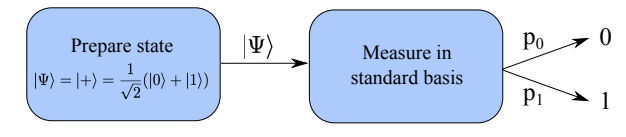
\includegraphics[width=1\linewidth]{../images/randomness.png}
    \caption{Genuine randomness from the preparation of a qubit in superposition}
    \label{fig:randomness}
\end{figure}
This simple example already tells us something about the power of quantum information: We could
build a machine that deterministically prepares the qubit $\ket{+}$, followed by a measurement in the
standard basis. Since $p_0=p_1=1/2$, this machine allows us to produce a perfect random number -
even though no randomness has been used inside our machine! In contrast, one can prove that no
classical deterministic machine can produce random numbers from scratch.

We saw how to measure a single qubit in the standard basis. The rule for computing probabilities
of measurement outcomes generalizes in a direct way to measuring n-qubit states. Indeed, consider
an n-qubit quantum state
\[
\ket{\Psi}=\sum_{x\in\{0,1\}^n} \alpha_x\ket{x}
\]
What happens when $\ket{\Psi}$ is measured in the standard basis $\ket{x}_x$? It turns out that the probability
of outcome x is given by $p_x = |\braket{x|\Psi}|^2=|\alpha_x|^2$, explaining again the need for normalization of
the vector $\ket{\Psi}$.

\subsubsection{Measuring a qubit in other bases}
Can we measure our qubit in any other basis? The answer to this is yes! Indeed this is another
feature that distinguishes quantum from classical, where the only basis around is the standard basis.
To find out how to analyze such a more general setting, let us first take a step back and consider
how we found the probabilities above. When measuring in the standard basis, the probabilities are given by the squared amplitudes when writing out the state in terms of the standard basis. When
measuring a qubit in a different orthonormal basis, given by vectors $\mathcal{G}=\{\ket{v},\ket{v^\perp}\}$, it is intuitive that we would have to express the qubit in the new basis. That is, we need to find amplitudes $\hat{\alpha}$ and $\hat{\beta}$ such that
\[
\ket{\psi}=\alpha\ket{0}+\beta\ket{1}=\hat{\alpha} \ket{v}+\hat{\beta}\ket{v^{\perp}}
\]
\begin{example}
    As an example, let consider again the qubit $\ket{+}=(1/\sqrt{2})(\ket{0}+\ket{1})$. Instead
of measuring it in the standard basis, let us now measure in the basis $H = \{\ket{+},\ket{-}\}$ given by
the two orthonormal vectors $\ket{+}$ and $\ket{-} = (1/\sqrt{2})(\ket{0}-\ket{1})$. Clearly, we can write the qubit as $1\ket{+}+0\ket{-}$. Thus the probability of obtaining measurement outcome “$\ket{+}$” is 1. We thus see
that the probabilities of measurement outcomes depends dramatically on the basis in which we
measure. 
\end{example}

\begin{example}
    Consider measuring an arbitrary qubit $\alpha\ket{0}+\beta\ket{1}$ in the basis $\{\ket{+},\ket{-}\}$. To
find out how to express the qubit in this other basis, it is convenient to determine how the basis
elements $\ket{0}$ and $\ket{1}$ look like in this basis. We find that
\[
\ket{0}=\frac{1}{2}[(\ket{0}+\ket{1})+(\ket{0}-\ket{1})]=\frac{1}{\sqrt{2}}(\ket{+}+\ket{-})
\]
\[
\ket{1}=\frac{1}{2}[(\ket{0}+\ket{1})-(\ket{0}-\ket{1})]=\frac{1}{\sqrt{2}}(\ket{+}-\ket{-})
\]
We thus have
\begin{align*}
\alpha\ket{0}+\beta\ket{1}&=\frac{1}{\sqrt{2}}[\alpha(\ket{+}+\ket{-})+\beta(\ket{+}-\ket{-})]\\
&=\frac{\alpha+\beta}{\sqrt{2}}\ket{+}+\frac{\alpha-\beta}{\sqrt{2}}\ket{-}
\end{align*}
This means that we obtain outcome "$\ket{+}$" with probability $|\alpha+\beta|^2/2$ and outcome "$\ket{-}$" with probability $|\alpha-\beta|^2/2$/
\end{example}

\begin{example}
    Consider the state $\ket{\Psi}=\ket{0}$. What are the probabilities  $p_0,p_1$ for measuring $\ket{\Psi}$ in the standard basis? What are the probability $p_{+},p_{-}$ for measuring $\ket{\Psi}$ in the Hadamard basis?
    For measuring in the standard basis the probabilities $p_0=1, p_1=0$. The probabilities in the Hadamard basis are $p_+=\frac{1}{2},p_-=\frac{1}{2}$.
\end{example}

Quite often we do not care about the entire probability distribution, but just the probability of one
specific outcome. Is there a more efficient way to find this probability than to rewrite the entire
state $\ket{\psi}$ in another basis? To investigate this, let us consider a single qubit
\[
\ket{\psi}=\alpha\ket{0}+\beta\ket{1}
\]
Remember that the elements of the standard basis are orthonormal. This means that
\[
(\ket{0})^{\dagger}\ket{0}=\begin{pmatrix} 1 & 0 \end{pmatrix}\begin{pmatrix} 1 \\ 0 \end{pmatrix} = 1,
\]
\[
(\ket{0})^{\dagger}\ket{1}=\begin{pmatrix} 1 & 0 \end{pmatrix}\begin{pmatrix} 0 \\ 1 \end{pmatrix} = 0
\]
Because the vectors are orthonormal, we could thus have found the desired probabilities by simply
computing the inner product between two vectors, as claimed above. Specifically, when given the qubit $\ket{\psi}=\alpha\ket{0}+\beta\ket{1}$ we obtain outcomes "$\ket{0}$" and "$\ket{1}$" with probabilities
\[
p_0=|\braket{0|\psi}|^2=\begin{vmatrix}\begin{pmatrix} 1 & 0 \end{pmatrix} \begin{pmatrix}\alpha \\ \beta \end{pmatrix}  \end{vmatrix}^2=|\alpha|^2
\]
\[
p_1=|\braket{1|\psi}|^2=\begin{vmatrix} \begin{pmatrix} 0 & 1 \end{pmatrix}\begin{pmatrix}\alpha \\ \beta \end{pmatrix}  \end{vmatrix}^2=|\beta|^2
\]

\begin{example}
    Suppose we measure $\ket{0}$ in the hadamard basis $\mathcal{H}$ (see above). The probabilities of observing outcomes "$\ket{+}$" and "$\ket{-}$" are given by
    \[
    p_+=|\braket{0|\psi}|^2=\begin{vmatrix}\begin{pmatrix} 1/\sqrt{2} & 1/\sqrt{2} \end{pmatrix} \begin{pmatrix}\alpha \\ \beta \end{pmatrix}  \end{vmatrix}^2=\frac{1}{2}
\]
\[
p_-=|\braket{1|\psi}|^2=\begin{vmatrix} \begin{pmatrix} 1/\sqrt{2} & 1/\sqrt{2} \end{pmatrix}\begin{pmatrix}\alpha \\ \beta \end{pmatrix}  \end{vmatrix}^2=\frac{1}{2}
\]
For multiple qubits, the rules for finding probabilities is analogous.
\end{example}

\begin{definition}
    Suppose that we measure a quantum state $\ket{\psi}$ in the orthonormal basis $\{\ket{b_j}\}_{j=1}^d$. The probability of observing outcome "$b_j$" can be found by computing
    \[
    p_j=|\braket{b_j|\psi}|^2
    \]
    The post-measurement state when obtaining outcome"$b_j$" is given by $\ket{b_j}$.
\end{definition}

Let us now consider some examples to gain intuition on measuring quantum systems in different
bases. First, let us have a look at a single qubit example.

\begin{example}
    Consider the qubit $\ket{\Psi}=\frac{1}{\sqrt{2}}(\ket{0}+\iota\ket{1})$, and measure the qubit in the $\{\ket{+},\ket{-}\}$ basis. the probabilities of obtaining "+" and "-" can be evaluated as follows:
    \begin{align*}
    p_+&=|\braket{\Psi|+}|^2=\begin{vmatrix} \dfrac{1}{2}(\bra{0}-\iota \bra{1})(\ket{0}+\ket{1})\end{vmatrix}^2\\
    &=\frac{1}{4}\begin{vmatrix} \braket{0|0}+\braket{0|1} - \iota\braket{1|0} - \iota \braket{1|1} \end{vmatrix}^2\\
    &=\frac{1}{4}|1-\iota|^2\\
    &=\frac{1}{4}(1-\iota)(1+\iota)=\frac{1}{2}
    \end{align*}
    \begin{align*}
    p_-&=|\braket{\Psi|-}|^2=\begin{vmatrix} \frac{1}{2}(\bra{0}-\iota \bra{1})(\ket{0}-\ket{1})\end{vmatrix}^2\\
    &=\frac{1}{4}\begin{vmatrix} \braket{0|0}+\braket{0|1} - \iota\braket{1|0} + \iota \braket{1|1} \end{vmatrix}^2\\
    &=\frac{1}{4}|1+\iota|^2\\
    &=\frac{1}{4}(1-\iota)(1+\iota)=\frac{1}{2}
    \end{align*}
\end{example}
This example shows that when the states involved have complex-valued amplitudes, one has to
take extra caution when evaluating the inner product: namely when taking the bra $\bra{\Psi}$, one should remember to alter the +/- sign whenever a complex number is involved (since the bra $\bra{\Psi}$ is the
conjugate transpose of the ket $\ket{\Psi}$). 

While we will generally talk about n-qubits, we can of course also consider a quantum system
comprised of three levels $\ket{0}$, $\ket{1}$, and $\ket{2}$, i.e. a qutrit. The rule for obtaining the probabilities of
measurement outcomes remains unchanged.

\begin{example}
    Consider a qutrit, which is a 3-dimensional quantum system represented by the vector
    \[
    \ket{v}=\frac{1}{\sqrt{2}}\begin{pmatrix} 1 \\ 0 \\ 0\end{pmatrix} + \frac{1}{\sqrt{2}}\begin{pmatrix} 0 \\ 1 \\ 0\end{pmatrix}\frac{1}{\sqrt{2}}\begin{pmatrix} 0 \\ 0 \\ 1\end{pmatrix}
    \]
    and measure in the basis $\mathcal{B}=\{\ket{b_1},\ket{b_2},\ket{b_3}\}$ where
    \[
    \ket{b_1}=\begin{pmatrix} 1 \\ 0 \\ 0 \end{pmatrix}, \quad \ket{b_2} = \frac{1}{\sqrt{2}}\begin{pmatrix} 0 \\ 1 \\ 1 \end{pmatrix}, \quad \frac{1}{\sqrt{2}}\begin{pmatrix} 0 \\ 1 \\ -1 \end{pmatrix} 
    \]
    The probabilities of obtaining each outcome can be calculated as follows:
    \[
    p_{b_1}=|\braket{b_1|v}|^2=\frac{1}{2}
    \]
    \[
    p_{b_2}=|\braket{b_2|v}|^2=\braket{b_2|v}\braket{v|b_2}=\frac{1}{2\sqrt{2}}(1+1)\frac{1}{2\sqrt{2}}(1+1)=\frac{1}{2}
    \]
    \[
    p_{b_3}=|\braket{b_3|v}|^2=\braket{b_3|v}\braket{v|b_3}|=\frac{1}{2\sqrt{2}}(1-1)\frac{1}{2\sqrt{2}}(1-1)=0
    \]
\end{example}

\subsubsection{Measurement Example I: Phase Estimation}
Now that we have discussed qubits in some detail, we can are prepared to
look more closesly at the measurement principle. Consider the quantum
state,
|\[
\ket{\psi}=\frac{1}{\sqrt{2}}\ket{0}+\frac{e^{\iota\theta}}{\sqrt{2}}\ket{1}
\]
If we were to measure this qubit in the standard basis, the outcome would
be $0$ with probability $1/2$ and $1$ with probability$ 1/2$. This measurement
tells us only about the norms of the state amplitudes. Is there any measurement that yields information about the phase, $\theta$?
To see if we can gather any phase information, let us consider a measurement in a basis other than the standard basis, namely
\[
\ket{+}=\frac{1}{\sqrt{2}}(\ket{0}+\ket{1}) \quad \text{and}\quad \ket{-}=\frac{1}{\sqrt{2}}(\ket{0}-\ket{1})
\]
What does $\ket{\phi}$ look like in this new basis? This can be expressed by first
writing,
\[
\ket{0}=\frac{1}{\sqrt{2}}(\ket{+}+\ket{-}) \quad \text{and} \quad \ket{-}=\frac{1}{\sqrt{2}}(\ket{0}-\ket{1})
\]
Now we are equipped to rewrite $\ket{\psi}$ in the $\{\ket{+}$, $\ket{-}\}$-basis,
\begin{align*}
\ket{\psi}&=\frac{1}{\sqrt{2}}\ket{0}+\frac{e^{\iota\theta}}{\sqrt{2}}\ket{1}\\
&=\frac{1}{2}(\ket{+}+\ket{-})+\frac{e^{\iota\theta}}{\sqrt{2}}(\ket{+}-\ket{-})\\
&=\frac{1+e^{\iota\theta}}{2}\ket{+}+\frac{1-e^{\iota\theta}}{2}\ket{-}
\end{align*}
Recalling the Euler relation, $e^{\iota theta}=\cos \theta+\iota\sin \theta$, we see that the probability
of measuring $\ket{+}$ is $\frac{1}{4}((1+\cos \theta)^2+\sin^2 \theta)=\cos^2 (\theta/2)$. A similar calculation reveals that the probability of measuring $\ket{-}$ is $\sin^2 (\theta/2)$ Measuring
in the ($ket{+},\ket{-}$)-basis therefore reveals some information about the phase $\theta$.
Later we shall show how to analyze the measurement of a qubit in a
general basis.

\subsubsection{Measurement example II: general Qubit Bases}
What is the result of measuring a general qubit state $\ket{\psi}=\alpha\ket{0}+\beta\ket{1}$, in
a general orthonormal basis $\ket{v}$, $\ket{v^{\perp}}$, where $\ket{v}=a\ket{0}+b\ket{1}$ and $\ket{v^{\perp}}=b^*\ket{0}-a^*\ket{1}$? You should also check that $\ket{v}$ and $\ket{v^{\perp}}$ are orthogonal by
showing that $\braket{v|v^{\perp}}=0$.

To answer this question, let us make use of our recently acquired braket notation. We first show that the states $\ket{v}$ and $\ket{v^{\perp}}$ are orthogonal, that is, that their inner product is zero:
\begin{align*}
\braket{v|v^{\perp}}&=(b^*\ket{0}-a^*\ket{1})^{\dagger}(a\ket{0}+b\ket{1})\\
&=(b\bra{0}-a\bra{1})^{\dagger}(a\ket{0}+b\ket{1})\\
&=ba\braket{0|0}-a^2\braket{1|0}+b^2\braket{0|1}-ab\braket{1|1}\\
&=ba-0+0-ab\\
&=0
\end{align*}

Here we have used the fact that $\braket{i|j}=\delta_{ij}$ .

Now, the probability of measuring the state $\ket{\psi}$ and getting $\ket{v}$ as a
result is,
\begin{align*}
p_{\psi}(v)&=|\braket{v|\psi}|^2\\
&=|(a^*\bra{0}+b^*\bra{1})(\alpha\ket{0}+\beta\ket{1})|^2\\
&=|a^*\alpha+b^*\beta|^2
\end{align*}
Similarly,
\begin{align*}
P_{\psi}(v^{\perp})&=|\braket{v^{\perp}|\psi}|^2\\
&=|(b\bra{0}-a\bra{1})(\alpha\ket{0}+\beta\ket{1})|^2\\
&=|b\alpha-\alpha\beta|^2
\end{align*}

\subsubsection{Expectation Values}
Physicists (but also computer scientists!) like to compute expectation values of measurement outcomes, as they provide an indication of the average behavior, if one was to perform a measurement many times (however we shall see later, that the measurement will perturb the state!). let us suppose that we measure a qubit $\ket{\Psi}$ in the standard basis $\{\ket{0},\ket{1}\}$. We will adopt the physics convention of labelling outcomes $\pm1$. This means that we associate the outcome "$\ket{0}$" with outcome $+1$, and outcome "$\ket{1}$" with outcome $-1$. The expectation value the outcome obtained when measuring $\ket{\psi}$ is then
\[
E=1|\braket{0|\psi}|^2-1\braket{1|\psi}|^2
\]
Note that since $|\braket{0|\psi}|^2=\braket{\psi|0}\braket{0|\psi}$, we have
\[
E=\bra{\psi}(\ket{0}\bra{0}-\ket{1}\bra{1})\ket{\psi}=\braket{\psi|Z|\psi}
\]
where $Z=\ket{0}\bra{0}-\ket{1}\bra{1}$.  As we shall see later, $Z$ is called the Pauli-Z matrix.

\subsection{Measuring Multiple Systems}
We saw how to measure some quantum state $\ket{\psi}$. let us now consider what happens if we measure the state of multiple qubits, where we think of measuring each qubit in a separate basis. To understand this, it is useful to realize that a basis for the join state space $\mathbb{C}_A^{d_A} \otimes \mathbb{C}_B^{d_B}$ can be obtained from bases for the individual state spaces $\mathbb{C}_A^{d_A}$ and $\mathbb{C}_B^{d_B}$. Specifically, if $\{\ket{b_j^A}\}_j$ is basis for $\mathbb{C}_A^{d_A}$ and $\{\ket{b_j^B}\}_j$ is a basis for the state space $\mathbb{C}_B^{d_B}$, then the set of vectors $\{\{\ket{b_j^A}\otimes \ket{b_k^B}\}_{j=1}^{d_A}\}_{k=1}^{d_B}$ gives a basis for $\mathbb{C}_A^{d_A}\otimes \mathbb{C}_B^{d_B}$.

\begin{example}
    Consider the basis $\{\ket{0}_A,\ket{1}_A\}$ for qubit A, and the basis $\{\ket{+}_B,\ket{-}_B\}$ for qubit B. A basis for the joint state AB is then given by $\{\ket{0}_A\ket{+}_B,\ket{0}_A\ket{-}_B,\ket{1}_A\ket{+}_B,\ket{1}_A\ket{-}_B\}$.
\end{example}

Let us not think how we might construct how we might construct some measurement for two quantum states from measurements of the individual ones. Suppose we measure particle A in the basis $\{\ket{b_j^A}\}_j$ and particle B in the basis $\{b_k^B\}_k$ when the joint state of both particles is given by $\ket{\psi}_{AB}$. What is the probability that we obtain outcome "$\ket{b_j^A}$" on A, and outcome "$\ket{b_k^B}$" on B? To find such joint probabilities, we first write down the joint basis fo quantum states A and B as above: $\{\{\ket{b_j^A}\ket{b_k^B}\}_j\}_k$. We can apply the usual rule to compute the probability as 
\[
p_{jk}=|\braket{b_j^A|\braket{b_k^B|\ket{\psi}_{AB}}}|^2
\]
\begin{example}
    Consider the two qubits in an EPR pair
    \[
    \ket{EPR}=\frac{1}{\sqrt{2}}(\ket{00}+\ket{11}
    \]
    and measure them both in the standard basis. The probabilities of obtaining outcomes 00, 01 ,10 and 11 are given by
    \[
    p_{00}=p_{11}=\frac{1}{2}
    \]
    \[
    p_{01}=p_{10}=0
    \]
\end{example}

\subsubsection{Partial Measurements}
Suppose we have a system consisting of two or more qubits and we only measure one of them. For
example, suppose the qubits are X and Y, and these qubits are in the state
\[
\ket{\psi}=\frac{1}{2}\ket{00}-\frac{\iota}{2}\ket{10}+\frac{1}{\sqrt{2}}\ket{11}
\]
We know what the distribution of measurement outcomes would be if we measured both qubits:
\[
Pr\text{[outcome is 00]} = \frac{1}{4} \quad Pr\text{[outcome is 01]}=0
\]
\[
Pr\text{[outcome is 10]}=\frac{1}{4} \quad pr\text{[outcome is 11]}=\frac{1}{2}
\]
The probability that a measurement of the first qubit, for instance, results in outcome $0$ should
therefore be $1/4+0 = 1/4$ and the probability of outcome $1$ should be $1/4+1/2 = 3/4$. Intuitively,
this should be the case regardless of whether or not the second qubit was actually measured. Indeed
this is the case.

However, what is different between the case where the second qubit is measured and the case
where it is not is the superposition of the system after the measurement (or measurements). If both
qubits are measured, the superposition will be one of $\ket{00},\ket{01},\ket{10}$, or $\ket{11}$, depending on the
measurement outcome. If only the first qubit is measured, however, this may not be the case.
I’ll explain how you determine the state of the system after the measurement of the first qubit
for the example above, and the method for a general case should be clear. We begin by considering
the possible outcome 0 for the measurement. We consider the state
\[
\ket{\psi}=\frac{1}{2}\ket{00}-\frac{\iota}{2}\ket{10}+\frac{1}{\sqrt{2}}\ket{11}
\]
and cross off all of the terms in the sum that are inconsistent with measuring a $0$ for the first qubit:
\[
\ket{\psi}=\frac{1}{2}\ket{00}
\]
which leaves
\[
\frac{1}{\ket{00}}
\]
The probability of measuring 0 is the norm-squared of this vector.
\[
Pr\text{[measurement outcomes is 0]}=|\\frac{1}{2}\ket{00}\|=\frac{1}{4}
\]
and the state of the two qubits after the measurement conditioned on the measurement outcome being 0 is the vector itself renormalized:
\[
frac{\frac{1}{2}\ket{00}}{\|\frac{1}{2}\ket{00}\|}=\ket{00}
\]
The possible measurement outcome 1 is handled similarly. we cross off the terms is inconsistent with measuring a 1 which leaves
\[
-\frac{\iota}{2}\ket{10}+\frac{1}{\sqrt{2}}\ket{11}
\]
The probability of measuring a 1 is then the norm-squared of this vector,
\[
Pr\text{measurement outcome is 1]}=\|-\frac{\iota}{2}\ket{10}+\frac{1}{\sqrt{2}}\ket{11}\|^2=|-\frac{\iota}{2}|^2+|\frac{1}{\sqrt{2}}|^2=\frac{3}{4}
\]
and conditioned on measuring a 1 is then the norm-squared of this vector
\[
\frac{-\frac{\iota}{2}\ket{10}+\frac{1}{\sqrt{2}}\ket{11}}{\|-\frac{\iota}{2}\ket{10}+\frac{1}{\sqrt{2}}\ket{11}\|}=-\frac{\iota}{\sqrt{3}}\ket{10}+\sqrt{\frac{2}{3}}\ket{11}
\]
A completely equivalent way of performing this calculation is to begin by writing
\[
\ket{\psi}=\ket{0}\ket{\phi_0}+\ket{1}\ket{\phi_1}
\]
for some choice of $\ket{\phi_0}$ and $\ket{\phi_1}$. (There will always be a unique choice for each that works.) in this case we have
\[
\ket{\psi}=\ket{0}\left(\frac{1}{2}\ket{0}\right)+\ket{1}\left(-\frac{\iota}{2}\ket{0}+\frac{1}{\sqrt{2}}\ket{1}\right)
\]
so $\ket{\phi_0}=\frac{1}{2}\ket{0}$ and $\ket{\phi_1}=-\frac{\iota}{2}\ket{0}+\frac{1}{\sqrt{2}}\ket{1}$. The probabilities for the two measurement outcomes are as follows:
\[
Pr\text{[outcome is 0]}=\|\ket{\phi_0}\|^2=|\frac{1}{2}|^2=\frac{1}{4}
\]
\[
Pr\text{[outcome is 1]}=\|\ket{\phi_1}\|^2=|-\frac{\iota}{2}|^2+|\frac{1}{\sqrt{2}}|^2=\frac{3}{4}
\]
Conditioned on the measurement outcome, the state of the two qubits is as follows:
\[
\text{measurement outcome is 0}\implies \text{state becomes} \frac{1}{\|\ket{\phi_0}\|}\ket{0}\ket{\phi_0}=\ket{00}
\]
\[
\text{measurement outcome is 1} \implies \text{state becomes}\frac{1}{\|\ket{\phi_1}}\ket{1}\ket{\phi_1}=\frac{-\iota}{\sqrt{3}}\ket{10}+\sqrt{\frac{2}{3}}\ket{11}
\]
The same method works for more than 2 qubits as well.

\begin{example}
    Suppose 3 qubits are in the superposition
    \[\ket{\psi}=\frac{1}{2}\ket{000}+\frac{1}{2}\ket{100}+\frac{1}{2}\ket{101}-\frac{1}{2}\ket{111}\]
    and the third qubit is measured. What are the probabilities of the two possible measurement outcomes and what are the resulting superpositions of the three qubits for each case?
    To determine the answer we ewrite,
    \[
    \ket{\psi}=\left(\frac{1}{2}\ket{00}+\frac{1}{2}\ket{10}\right)\ket{0}+\left(\frac{1}{2}\ket{10}-\frac{1}{2}\ket{11}\right)\ket{1}
    \]
    The probability that the measurement outcome is 0 is
    \[
    \|\frac{1}{2}\ket{00}+\frac{1}{2}\ket{10}\|^2=\frac{1}{2}
    \]
    and in this case the resulting superposition is 
    \[
    \sqrt{2}\left(\frac{1}{2}\ket{00}+\frac{1}{2}\ket{10}\right)\ket{0}=\frac{1}{\sqrt{2}}\ket{000}+\frac{1}{\sqrt{2}}\ket{100}
    \]
    The probability that the measurement outcome is 1 is
    \[
    \|\frac{1}{2}\ket{10}-\frac{1}{2}\ket{11}\|^2=\frac{1}{2}
    \]
    and in this case the resulting superposition is
    \[
    \sqrt{2}\left(\frac{1}{2}\ket{10}-\frac{1}{2}\ket{11}\right)\ket{1}=\frac{1}{\sqrt{2}}\ket{101}-\frac{1}{\sqrt{2}}\ket{111}
    \]
\end{example}









\chapter{Axioms of Quantum Mechanics}
\subsection{Postulate 1: The State Space Postulate}
The state of an isolated quantum mechanical system is completely specified by a state vector $\ket{\psi}$ 
which is a unit vector that belongs to a complex vector space with inner product (a Hilbert Space) $\mathbb{C}^{n}$, where $n$ is the 
dimension of the state space of the system. 

Consider some physical system that can be in N different, mutually exclusive classical states (it means a state in which the system can be found 
if we observe it) $\ket{0},\ket{1},\ldots,\ket{N-1}$. Then, a \textit{pure quantum state} (or \textit{state}) $\ket{\psi}$ is a superposition of classical states, written as:
\[
    \ket{\psi}=\alpha_0\ket{0}+\alpha_1\ket{1}+\ldots+\alpha_{N-1}\ket{N-1} = \sum_{i=0}^{N-1}\alpha_i\ket{i}
\]
where $\alpha_i$ are complex numbers called amplitude of $\ket{i}$ in $\ket{\psi}$. A system in quantum state
$\ket{\psi}$ is in a superposition of the classical states $\ket{0},\ket{1},\ldots,\ket{N-1}$ with amplitudes $\alpha_0,\alpha_1,\ldots,\alpha_{N-1}$ respectively.
Mathematically, the states $\ket{0}$, $\ket{1}$, $\ldots$, $\ket{N-1}$ forms an N-dimensional Hilbert space (i.e. N dimensional complex vector space with inner product defined).
We write the quantum state $\ket{\psi}$ as a N-dimensional column vector of its amplitudes in the Hilbert Space.
\[ 
    \ket{\psi}=\begin{pmatrix} \alpha_0 \\ \alpha_1 \\ \vdots \\ \alpha_{N-1} \end{pmatrix}
\]
Consider a Hilbert space $\mathcal{H_A}$ with orthonormal basis $\ket{0},\ket{1},\ldots,\ket{N-1}$
and another Hilbert space $\mathcal{H_B}$ with an orthonormal basis $\ket{0'},\ket{1'},\ldots,\ket{M-1}$. Then we can
combine the two Hilbert spaces using tensor products to form a new Hilbert space $\mathcal{H}=\mathcal{H_A}\otimes\mathcal{H_B}$ which
is a $N\times M$ dimensional Hilbert space with basis $\ket{i}\otimes\ket{j}$ where $\ket{i}$ is a basis vector of $\mathcal{H_A}$ ($\ket{i} \in \{0,\ldots,N-1\}$) 
and $\ket{j}$ is a basis vector of $\mathcal{H_B}$ ($\ket{j} \in \{0',\ldots,M-1\})$. The basis vectors of $\mathcal{H}$ are $\ket{i}\otimes\ket{j}$ where $i \in \{0,\ldots,N-1\}$ and $j \in \{0',\ldots,M-1\}$.
Thus, an arbitrary state of $\mathcal{H}$ can be written as:
\[
    \ket{\psi}=\sum_{i=0}^{N-1}\sum_{j=0'}^{M-1}\alpha_{ij}\ket{i}\otimes\ket{j}
\]
where $\alpha_{ij}$ are complex numbers called amplitudes of $\ket{i}\otimes\ket{j}$ in $\ket{\psi}$.
Sucg as state is called $\mathit{bipartite}$. Similarly, this can be extended to tripartite states which is a tensor product of three Hilbert spaces and so on.

The simplest system is qubit - a quantum mechanical system with two-dimensional state space. Suppose $\ket{0}$ and
$\ket{1}$ are two orthonormal basis vectors also generally called as \textbf{computational basis} of the state space of the qubit. Then the arbitrary state of the qubit can be represented as
\[
    \ket{\psi}=\alpha\ket{0}+\beta\ket{1}
\]
where $\alpha$ and $\beta$ are complex numbers such that $|\alpha|^2+|\beta|^2=1$ (since its a unit vector). The condition 
$|\alpha|^2+|\beta|^2=1$ is called the \textit{normalization condition}. The complex numbers $\alpha$ and $\beta$ are called probability amplitudes
for the states $\ket{0}$ and $\ket{1}$ respectively.

Intuitively, one can think of the state $\ket{0}$ and $\ket{1}$ as the analogous to the classical bit states $0$ and $1$. 
The qubit differs from the classical bit in the sense that the qubit can exist in a superposition of the states $\ket{0}$ and $\ket{1}$,
i.e. of the form $\alpha\ket{0}+\beta\ket{1}$ where $\alpha$ and $\beta$ are complex numbers, which is neither in state $\ket{0}$ or in $\ket{1}$ (or in both the sates 
simultaneously)  which does not happen for a classical bit. This is the essence of quantum superposition which can be taken advantage of in quantum computing.

\begin{example}
    A qubit can exist in a state such as 
    \[\dfrac{\ket{0}-\ket{1}}{\sqrt{2}}\]
    which is a superposition of the states $\ket{0}$ and $\ket{1}$ with amplitude $1/\sqrt{2}$ for being in state $\ket{0}$ and 
    amplitude $-1/\sqrt{2}$ for being in the state $\ket{1}$.
\end{example}
\begin{example}
    Say a state of a qubit is $\ket{\psi}=7\ket{0}+(3+5\iota)\ket{1}$. In the matrix form, it can be written as:
    \[
        \ket{\psi}=\begin{pmatrix} 7 \\ 3+5\iota \end{pmatrix}
    \]
\end{example}

In general we say that any linear combination $\sum_i \alpha_i \ket{\psi_i}$ is a superposition of the states $\ket{\psi_i}$ with amplitudes 
$\alpha_i$ for the state $\ket{\psi_i}$.

\textbf{There are two things we can do with a quantum state: Measure it or let it evolve (without measuring it).}

\subsection{Postulate 2: Evolution Postulate}\label{subsection:Postulate 2}
The time evolution of a closed Quantum System is described by the Schrodinger equation as:
\[
    i\hbar\frac{d}{dt}\ket{\psi(t)}=H\ket{\psi(t)}
\]
where $\ket{\psi(t)}$ is the state of the system at time $t$, $H$ is the Hamiltonian operator of the system and $\hbar$ is the reduced Planck's constant.
The Hamiltonian operator is an operator that corresponds to the total energy of the system. The Schrodinger equation is a linear differential equation and is the quantum analog of Newton's second law of motion.
The solution to the Schrodinger equation gives the state of the system at any time $t$ given the initial state of the system.
If we know the Hamiltonian of a system, we can predict the future state of the system. For the purpose of Quantum computing, we are interested in the time evolution of a quantum system. Thus, we will
always assume that the Hamiltonian of a quantum system is known. Thus, simplifying the Schrodinger equation, we can write it as:
\[
    \frac{d}{dt}\ket{\psi(t)}=-\frac{i}{\hbar}H\ket{\psi(t)}
\]
Rearranging the above equation, we get:
\[
    \int_{\psi_{t_1}}^{\psi_{t_2}} \frac{d\ket{\psi}}{\ket{\psi}}=-\int_{t_1}^{t_2}\frac{i}{\hbar}Hdt
\]
Integrating, the above equation we get,
\[
    \ln\left(\frac{\ket{\psi_{t_2}}}{\ket{\psi_{t_1}}}\right)=-\frac{i}{\hbar}H(t_2-t_1)
\]
\[\ket{\psi_{t_2}}=e^{-\frac{i}{\hbar}H(t_2-t_1)}\ket{\psi_{t_1}}\]
Now we know that the Hamiltonian operator H is Heritian and as proved in the appending we know that $e^{A}$ is unitary for any Heritian operator A.
Thus, the time evolution operator $U(t_2,t_1)=e^{-\frac{i}{\hbar}H(t_2-t_1)}$ is unitary.
Hence, we can write the time evolution of a quantum state as:
\[
    \ket{\psi(t_2)}=U(t_1,t_2)\ket{\psi(t_1)}
\]
where U is a Unitary time evolution Operator. Thus, we have described a discrete time desciption of the dynamics using unitary operators.
For the purpose of Quantum Computing, we will deal with discrete time evolution of the quantum system described by the exponenetial of the Hamiltonian (Hermitian operator) 
which is a unitary operator as shown and not the continuous time evolution of the quantum system described by the hamitlonian. Thus, we restate the postulate for Quantum Computing as:
\textbf{The evolution of a closed quantum system is described by a Unitary transformation. That is, the two states at times $t_1$ and time $t_2$ are related by
a unitary operator $U(t_2,t_1)$ such that $\ket{\psi(t_2)}=U(t_2,t_1)\ket{\psi(t_1)}$}.

\textbf{Note that in quantum computing we oftern apply a unitary operator to a closed quantum state. This is contradictory statement.
The act of applying a unitary operator is in itself an external iteraction with the quantum system, thus it no longer remains closed. 
It turns out, that it is possible to write down a time-varying Hamiltonian for a Quantum system, in which the hamiltonian for the system is not constant,
but varies according to some external control parameters which are under experimentalist's control, and could be changed during the 
course of an experiment. The system is therefore not closed, but it does evolve according to Schrdinger's equation with a time varying Hamiltonian, to some good
approximation. Thus we will describe the evolutions of a quantum system even those system's which aren't closed using unitary operators.}

\subsection{Postulate 3: Measurement Postulate}
\textbf{Measurement in the computational basis}\\
Consider a Quantum System in a state $\ket{\psi} = \sum_{j=0}^{N-1} \alpha_j \ket{j}$ which is some unknown superposition of the classical states $\ket{j}$. We cannot know exactly what the superposition of the states $\ket{\psi}$ is
since we can see only the classical states. Thus if we measure the state $\ket{\psi}$ it will collapse to one of the classical states
(say $\ket{j}$). To which classical state will it collapse to (which will we see)? This is not known in advance, we can
only predict the probabiltiy of the state collapsing to a particular classical state. The probability of the state $\ket{\psi}$ collapsing to the classical state $\ket{j}$ is given by
\textbf{Born's Rule} as:
\[
    P(j)=|\braket{j|\psi}|^2=|\alpha_j|^2
\]
where $\alpha_j$ is the amplitude of the state $\ket{j}$ in the state $\ket{\psi}$. Thus, the probability of the state $\ket{\psi}$ collapsing to the classical state $\ket{j}$ is the square of the amplitude of the state $\ket{j}$ in the state $\ket{\psi}$.
Now, since its a probability distribution this implies that the sum of the probabilities of the state $\ket{\psi}$ collapsing to any of the classical states $\ket{j}$ is 1. Thus, we have:
\[
    \sum_{j}P(j)=\sum_{j}|\alpha_j|^2=1
\]
thus, $\alpha_j$ are called probability amplitudes. (\textbf{Note that since operations on a quantum state are unitary in nature and 
a Unitary operator as shown in the appendix preserves norm, thus once the amplitudes are normalized to satisfy the Born's rule we can be sure that the probabilities will remain normalized no matter the number
of times we perform any unitary operation on the quantum state}). Once we measure the state 
$\ket{\psi}$ and it collapses to the classical state $\ket{j}$, the state of the system is now $\ket{j}$ and all the information that might have been contained in the amplitudes of $\alpha_i$ is gone.

Note that the probabilities of various measurement outcomes are exactly the same when we measure $\ket{\psi}$ or when we measure 
the state $e^{\iota \theta}\ket{\psi}$. The term $e^{\iota \theta}$ is called the \textbf{global phase} and thus has no physical significance.

Note that when the exprimentalist and their experimental apparatus observes the system,it is an external physical system in other words, and the interaction
makes the quantum system no longer closed and thus not necessarily subject to the unitary evolution. Thus, more formally we can state the postulate as: \\
\textbf{Quantum measurements are descibed by a collection $\{M_m\}$ of measurement operators.
These are operators acting on the state space $\ket{\psi}$ being meaured. The index m refers to the measurement outcomes 
that may occur in the experiment. If the state of the quantum system is $\ket{\psi}$ immediately before the measurement then the probability that result m
occurs is given by: 
\[
    p(m)=\bra{\psi}M_m^{\dagger}M_m\ket{\psi}
\]
and the state of the system after the measurement is:
\[
    \dfrac{M_m\ket{\psi}}{\sqrt{p(m)}}
\]
Now since the sum of the probabilities of all the measurement outcomes is 1, we have:
\[
    1 = \sum_m p(m) = \sum_m \bra{\psi}M_m^{\dagger}M_m\ket{\psi}
\]
Thus, the measurement operators satisfy the completeness equation:
\[
    \sum_m M_m^{\dagger}M_m=I
\]
}

\begin{example}
    Measurement of a qubit in the computational basis. Measurement of a qubit with two outcomes defined by the two measruremnt
    operators $M_0=\ket{0}\bra{0}$ and $M_1=\ket{1}\bra{1}$ (note that both the measurement operators are Hermitian and $M_0^2=M_0,M_1^2=M_1$, thus follow Completeness relation).
    Suppose the qubit is in the state $\ket{\psi}=\alpha\ket{0}+\beta\ket{1}$. The probability of the qubit collapsing to the state $\ket{0}$ is:
    \[
        p(0)=|\braket{0|\psi}|^2=|\alpha|^2
    \]
    and the probability of the qubit collapsing to the state $\ket{1}$ is:
    \[
        p(1)=|\braket{1|\psi}|^2=|\beta|^2
    \]
    Thus, the state of the qubit after the measurement is:
    \[
        \dfrac{M_0\ket{\psi}}{\sqrt{p(0)}}=\dfrac{\alpha\ket{0}}{|\alpha|}
    \]
    \[ 
        \dfrac{M_1\ket{\psi}}{\sqrt{p(1)}}=\dfrac{\beta\ket{1}}{|\beta|}
    \]
\end{example}


\begin{example}
    Consider a state $\ket{\psi}=\left(\frac{1}{\sqrt{6}}-\frac{1}{\sqrt{3}}\right)\ket{+}+\left(\frac{1}{\sqrt{6}}+\frac{1}{\sqrt{3}}\right)\ket{-}$ (it can be given in any basis, say here it is given in hadamard basis).
    Find the probabilities of measurement in Hadamard basis and Standard basis.\\
    Probability of measuring the state $\ket{\psi}$ in Hadamard basis to be $\ket{+}$ is:
    \[
        p(+)=|\braket{+|\psi}|^2=|\left(\frac{1}{\sqrt{6}}-\frac{1}{\sqrt{3}}\right)|^2=\frac{1}{6}+\frac{1}{3}-\frac{2}{\sqrt{18}}=\frac{3-2\sqrt{2}}{6}
    \]
    Probability of measuring the state $\ket{\psi}$ in Hadamard basis to be $\ket{-}$ is:
    \[
        p(-)=|\braket{-|\psi}|^2=|\left(\frac{1}{\sqrt{6}}+\frac{1}{\sqrt{3}}\right)|^2=\frac{1}{6}+\frac{1}{3}+\frac{2}{\sqrt{18}}=\frac{3+2\sqrt{2}}{6}
    \]
    Probability of measuring the state $\ket{\psi}$ in Standard basis to be $\ket{0}$ is:
    \[
        p(0)=|\braket{0|\psi}|^2=|\frac{1}{\sqrt{2}}\left(\frac{2}{\sqrt{6}}\right)|^2=|\frac{1}{\sqrt{3}}|^2=\frac{1}{3}
    \]
    Probability of measuring the state $\ket{\psi}$ in Standard basis to be $\ket{1}$ is:
    \[
        p(1)=|\braket{1|\psi}|^2=|\frac{1}{\sqrt{2}}\left(\frac{2}{\sqrt{3}}\right)|^2=|\frac{\sqrt{2}}{\sqrt{3}}|^2=\frac{1}{3}
    \]
\end{example}

\begin{importantnote}
    \textbf{Distinguishing Non-Orthogonal States}
    \begin{theorem}
        Non-orthogonal states can't be reliably distinguished.
    \end{theorem}
    Consider two people Alice and Bob. Alice prepares a quantum state $\ket{\psi_i}$ ($1\leq i\leq n$) from some fixed set of states known to both parties and sends it to Bob . Bob has to determine which state Alice sent him.

    Suppose the states $\ket{\psi_i}$ are orthonormal. Then Bob can measure the state $\ket{\psi_i}$ using the following procedure. Define Measurement operators, $M_i=\ket{\psi_i}\bra{\psi_i}$, one for each possible index i, and an additional 
    measurement operator $M_0=I-\sum_{i=1}^{n}\ket{\psi_i}\bra{\psi_i}$. The measurement operators satisfy the completeness relation $\sum_{i=0}^{n}M_i^{\dagger}M_i=I$. Thus, for a state $\ket{\psi_i}$ then $p(i)=\bra{\psi_i}M_i\ket{\psi_i}=1$, so the result i occurs
    with certianinty. Thus, it is possible to reliably distinguish the orthonormal states $\ket{\psi_i}$.

    Suppose the states $\ket{\psi_i}$ are not orthonormal. then we can prove that there is no quantum measurement 
    capable of ditinguishing the quantum states. The idea is that Bob will do a measurement described by measurement operators $M_j$ with 
    outcome j. Depending on the outcome of the measurment Bob tries to guess what the index i was using some rule,
    $i=f(j)$ (where $f(\cdot)$ is the rule to make the guess). Bob can't distinguish between the states $\ket{\psi_1}$ and $\ket{\psi_2}$ 
    is because $\ket{\psi_2}$ can be decomposed intoa (non-zero) component parallel to $\ket{\psi_1}$, and a component orthogonal to $\ket{\psi_1}$.
\end{importantnote}


\subsubsection{Projective Measurements}
A special case of the general measurement postulate. Consider a Quantum System with quantum state $\ket{\psi}$. A projective measurement on some space, with m possible outcomes, is a collection of projectors.
$P_1,\ldots,P_m$ that all act on tha same space and sum to identity $\sum_{j=1}^m P_j=I$. These projectors are \textit{pairwise orthogonal},
$P_iP_j=\delta_{ij}P_i$ where $\delta_{ij}$ is the Kronecker delta. The Projector $P_j$ projects onto some subspace $V_j$ of the total Hilbert Space $V$. 
Now every state $\ket{\psi} \in V$ can be decomposed in a unique way as $\ket{\psi}=\sum_{j=1}^m P_j\ket{\psi}$. Note that since the projectors
are orthogonal, the subspaces $V_j$ are orthogonal and the projection of the states onto $V_j$. When we apply this measurement onto the pure
state $\ket{\psi}$, then we will get outcome j with probability $p(j)=\bra{\psi}P_j\ket{\psi}$. If the outcome j occurs, then the state of the systema
immediately after the measurement is $\dfrac{P_j\ket{\psi}}{\sqrt{p(j)}}$. Note that the probabilities sum to 1.
\textbf{We cannot chose which $P_j$ will be applied to the state but can only give a probability distribution. However, if the state $\ket{\psi}$ fully lies within
one of the subspaces $V_j$ then the measurement of the outcome will be j with certaining}
\textbf{Note that the m projectors together form one measurement, we don't use the word "measurement" for individual $P_j$.}
\begin{example}
    A measurement in the computational basis in a N-dimensional state space is a specific projective measurement
    with m=N and $P_j=\ket{j}\bra{j}$. $P_j$ projects onto the computation basis state $\ket{j}$ and the corresponding
    subspace $V_j \subset V$  is the 1-dimensional subspace spanned by $\ket{j}$. 
    Consider the state $\ket{\psi} = \sum_{j=0}^{N-1} \alpha_j \ket{j}$. $P_j\ket{\psi}=\alpha_j\ket{j}$, so applying our measurement
    will give outcome j with probability $|\alpha_j|^2$ and the state of the system after the measurement will be $\ket{j}$.
\end{example}


\begin{example}
    Note that we can choose any orthonormal basis for the projective measurement. For example, consider
    a quantum state $\ket{\psi}$ expressed as superposition of standard orthonormal basis states $\ket{0},\ket{1},\ldots,\ket{N-1}$. 
    We can choose any other orthonormal basis B of states say $\ket{\phi_0},\ket{\phi_1},\ldots,\ket{\phi_{N-1}}$
    and consider the projective measurement defined by the projectors $P_j=\ket{\phi_j}\bra{\phi_j}$.
    This is called measureing in B basis. Applying this measurement to the state $\ket{\psi}$ will give 
    outcome j with probability $|\braket{\phi_j|\psi}|^2$ and the state of the system after the measurement will be $\ket{\phi_j}$.
    Note that if $\ket{\psi}$ equals to one the basis vectors $\ket{\phi_j}$ then the measurement
    gives outcome j with probability 1.
\end{example}

\begin{example}
    Note that it is not at all necessary for projectors to be of rank 1. For example, we can consider only two projectors on a 
    N (even) dimensional space such that $P_1=\sum_{j<N/2} \ket{j}\bra{j}$ and $P_2=\sum_{j\geq N/2} \ket{j}\bra{j}$. say the state
    of a quantum system is $\ket{\psi}=\frac{1}{\sqrt{3}}\ket{1}+\sqrt{\frac{2}{3}}\ket{N}$. Then,
    it gives outcome 1 with probability $p(1)=\bra{\psi}P_1\ket{\psi}=\frac{1}{3}$ and outcome 2 with probability $p(2)=\bra{\psi}P_2\ket{\psi} = \frac{2}{3}$.

\end{example}

\textbf{Observables: }We can write projective measurements with operators $P_1,\ldots,P_m$ and associated 
distinct outcomes $\lambda_1,\lambda_2,\ldots,\lambda_m \in \mathbb{R}$, can be written as one Matrix $M=\sum_{i=1}^m \lambda_iP_i$ which
is called an observable. It has an advantage that the expected (average) value of the outcome can be easily calculated as $\bra{\psi}M\ket{\psi}$.
NOte that M is Hermitian. Every observable is a Hermitian.

\begin{definition}
    Projective Measurement: A projective measurement is a measurement described by an observable M, a Hermitian operator on the state space of the system
    being observed. Since, its a Hermitian operator hence has a spectral decomposition as:
    \[M=\sum_m mP_m\]
    where $P_m$ is the projection onto the eigen space of M with eigen value m. 
    \textbf{The possible outcomes of the measurement correspond to the eigenvalues, m, of the observable}. Upon,
    measuring the state $\ket{\psi}$, the probability of getting result m is given by:
    \[p(m)=\bra{\psi}P_m\ket{\psi}\]
    Given that the outcome m occured, the state of the quantum system immediately after the measurement is:
    \[\dfrac{P_m\ket{\psi}}{\sqrt{p(m)}}\]
\end{definition}

\textbf{Projective measurement as a special case of Postulate 3: Suppose measurement operators in Postulate 3 in addition to satisfying the 
completeness relation $\sum_m M_m^{\dagger}M_m=I$ also satisfy the relation that $M_m$ are orthogonal projectors, that is $M_m^{\dagger}=M_m$
hence are Hermitian. Then, the Postulate 3 reduces to a Projective measurement as defined.}
Calculation of Average values for Projective measurements. By defintion, the average value of the measurement is:
%Mutliline equation
\begin{align*}
    \mathbf{E}(M) &= \sum_m m p(m) \\
    &= \sum_m m \bra{\psi}P_m\ket{\psi} \\
    &= \bra{\psi}\left(\sum_m mP_m\right)\ket{\psi} \\
    &= \bra{\psi}M\ket{\psi}\\
    \braket{M}&=\bra{\psi}M\ket{\psi}
\end{align*}

\subsubsection{Postive Operator Valued Measure (POVM) measurements}
For some applications, the post-measurement of the state is of little interest. We only care about the final probability distribution 
on the m-outcomes, then we can use the most general type of measrurement called \textit{positive-operator-valued-measrue (POVM)}. For example,
when the system is measured only once, at the end. In such cases, the POVM measurement is more general than the projective measurement.

We specify m positive semi-definite (Psd) matrices $E_1,\ldots,E_m$ such that $\sum_m E_m=I$. When measuring a state 
$\ket{\psi}$, the probability of the outcome i is given by $Tr(E_i\ket{\psi}\bra{\psi}) = \bra{\psi}E_i\ket{\psi}$. A projective measurement is a special case of POVm where the 
measurement elements $E_i$ are projectors. (That is $E_i^2=E_i$ and $E_i^{\dagger}=E_i$). The POVM elements $E_i$ are not necessarily orthogonal. 
\textit{One can show that every POVM can be simulated by a projective measusrement on a slightly larger space that yields the exact probability distribution over measurement outcomes (Neumark's theoerem)}

\begin{example}
    Suppose in a 2-dimensional state space, we know that it is either in state $\ket{0}$ or $\ket{+}=\frac{1}{\sqrt{2}}(\ket{0}+\ket{1})$.
    Clearly, this two states are not orthogonal, so there is no measurement that distinguishes them perfectly. However, there is a POVm measurement that never makes a mistake,
    but sometimes gives another outcome 2, meaning "I don't know". That is, you would like to do a meaurement with three possible outcomes: 0,1 and 2, such that:
    \begin{itemize}
        \item If the state is $\ket{0}$, then you get a correct outcome 0 with proabability $1/4$ and outcome 2 with 
        probability $3/4$ but never get inncorrect outcome 1.
        \item If the state is $\ket{+}$, then you get correct outcome 1 with probability $1/4$ and outcome 2 with probabiltiy $3/4$ but never get the inncorrect outcome 0.
    \end{itemize}
    This cannot be achieved with projective measurement on the qubit, but can be achieved with follwoing 3-outcome POVM:
    \begin{itemize}
        \item $E_0=\frac{1}{2}\ket{-}\bra{-}$, (where $\ket{-}=\frac{1}{\sqrt{2}}(\ket{0}-\ket{1})$ which is orthogonal to the $\ket{+}$ state.)
        \item $E_1=\frac{1}{2}\ket{1}\bra{1}$ (note that this is orthogonal to the sate $\ket{0}$ state)
        \item $E_I-E_0-E_1$
    \end{itemize}
    Here $E_0,E_1,E_2$ are all psd and add up to identity, so they forma  valid POVM. None of the three matrices are projectors. (note the success probability can be improved further).
\end{example}
\begin{definition}
    Positive Operator Valued Measure (POVM): Suppose a measurement is described by measurement operator $M_m$ is performed upon a quantum state $\ket{\psi}$. Then the probability of 
    the outcome m is given by $p(m)=\bra{\psi}M_m^{\dagger}M_m\ket{\psi}$. Suppose we define $E_m=M_m^{\dagger}M_m$, then clearly $E_m$ is a positive operator. A POVM measurement is a measurement described by a set of measurement operators $\{E_m\}$ that satisfy the 
    completeness relation $\sum_m E_m=I$ and $p(m)=\bra{\psi}E_m\ket{\psi}$. Thus set of operators $E_m$ are sufficient to determine the probabilities of the differnt measurement outcomes.
    The operators $E_m$ are known as the POVM elements associated with the measurement. The complete set $\{E_m\}$ is known as POVM.
\end{definition}

\subsection{Postulate 4: Composite Systems}
Consider a composite system amde up of two or more distinct quantum physical systems.
What are the states of the composite system? How the state space of a composite system is built up from the state spaces of the component 
systems.
\begin{definition}
    The state space of a composite physical system is the tensor product of the state spaces of the component physial systems. Say, 
    if the systems are numbered through 1 to n and the system number i is prepared in the state $\ket{\psi_i}$ then the joint
    state of the total system is $\ket{\psi_1}\otimes\ket{\psi_2}\otimes\ldots\otimes\ket{\psi_n}$. This is called the tensor product state of the component states.    
\end{definition}

\begin{example}
    Consider the orthonormal basis vectors of a single qubit system $\ket{0}$ and $\ket{1}$. Then the orthonormal basis vectors of a two qubit system are:
    \[ \ket{0} \otimes \ket{0} = \begin{pmatrix} 1 \\ 0 \end{pmatrix} \otimes \begin{pmatrix} 1 \\ 0 \end{pmatrix} = \begin{pmatrix} 1 \begin{pmatrix} 1 \\ 0 \end{pmatrix} \\ 0 \begin{pmatrix} 1 \\ 0 \end{pmatrix} \end{pmatrix} = \begin{pmatrix} 1 \\ 0 \\ 0 \\ 0 \end{pmatrix} \]
    \[ \ket{0} \otimes \ket{1} = \begin{pmatrix} 1 \\ 0 \end{pmatrix} \otimes \begin{pmatrix} 0 \\ 1 \end{pmatrix} = \begin{pmatrix} 1 \begin{pmatrix} 0 \\ 1 \end{pmatrix} \\ 0 \begin{pmatrix} 0 \\ 1 \end{pmatrix} \end{pmatrix} = \begin{pmatrix} 0 \\ 1 \\ 0 \\ 0 \end{pmatrix} \]
    \[ \ket{1} \otimes \ket{0} = \begin{pmatrix} 0 \\ 1 \end{pmatrix} \otimes \begin{pmatrix} 1 \\ 0 \end{pmatrix} = \begin{pmatrix} 0 \begin{pmatrix} 1 \\ 0 \end{pmatrix} \\ 1 \begin{pmatrix} 1 \\ 0 \end{pmatrix} \end{pmatrix} = \begin{pmatrix} 0 \\ 0 \\ 1 \\ 0 \end{pmatrix} \]
    \[ \ket{1} \otimes \ket{1} = \begin{pmatrix} 0 \\ 1 \end{pmatrix} \otimes \begin{pmatrix} 0 \\ 1 \end{pmatrix} = \begin{pmatrix} 0 \begin{pmatrix} 0 \\ 1 \end{pmatrix} \\ 1 \begin{pmatrix} 0 \\ 1 \end{pmatrix} \end{pmatrix} = \begin{pmatrix} 0 \\ 0 \\ 0 \\ 1 \end{pmatrix} \]
Thus, $\ket{00},\ket{01},\ket{10},\ket{11}$ are the orthonormal basis vectors of the two qubit Quantum System. Thus, the state of a particle for a two qubit quantum mechanical system can be written as 
$\ket{\psi}=\alpha\ket{00}+\beta\ket{01}+\gamma\ket{10}+\delta\ket{11}$ where $\alpha,\beta,\gamma,\delta$ are complex numbers such that $|\alpha|^2+|\beta|^2+|\gamma|^2+|\delta|^2=1$ and in the matrix form it can be written in matrix form as:
\[
    \ket{\psi}=\begin{pmatrix} \alpha \\ \beta \\ \gamma \\ \delta \end{pmatrix}
\]
Thus, say if $\ket{\psi}=\begin{pmatrix} 7 \\ 0 \\ \iota +3 \\ 0 \end{pmatrix}$ then the state of the two qubit system is $\ket{\psi}=7\ket{00}+(\iota+3)\ket{10}$.
\end{example}
This, same concept of representing two-quibt quantum mechanical systems can also be extended to n-qubit quantum mechanical systems. It will be a vector in a $2^n$-dimensional complex vector space.
For example, in three dimensional vector space there will be $2^3=8$ basis vectors $\ket{000},\ket{001},\ket{010},\ket{011},\ket{100},\ket{101},\ket{110},\ket{111}$.
$\ket{101}$ will be represented in matrix form as:
\[
    \ket{101}=\begin{pmatrix} 0 \\ 1 \\ 0 \\ 0 \\ 0 \\ 1 \\ 0 \\ 0 \end{pmatrix}
\]


\subsubsection{Full and Partial Measurements of a multi-particle systems}
A full measurement is a measurement that is performed on all the particles of a multi-particle system.
A partial measurement is a measurement that is performed on some of the particles of a multi-particle system.
Recal that when we measure a particle in the computational basis it collapses to one of the classical states.
\begin{example}
    Consider a two qubit system in the state $\ket{\psi}=\alpha\ket{00}+\beta\ket{01}+\gamma\ket{10}+\delta\ket{11}$.
    A full measurement on the two qubit system will give the outcome 00 with probability $|\alpha|^2$, outcome 01 with probability $|\beta|^2$, outcome 10 with probability $|\gamma|^2$ and outcome 11 with probability $|\delta|^2$. Thus, also note that 
    the sum of the probabilities of all the outcomes is 1, it is assumed the the state is initially normalized ($|\alpha|^2+|\beta|^2+|\gamma|^2+|\delta|^2=1$).
    
    A partial measurement on the two qubit system is a measurement performed on one of the qubits. Say, we perform a measurement on the first qubit, then the state of the second qubit will be the state of the system after the measurement on the first qubit.
    
    Suppose on measurement of the first qubit the probability that it collapsed to state 1 is given by $|\gamma|^2+|\delta|^2$ which is probabiltiy that the state collapses to $\ket{10}$ i.e. $|\gamma|^2$ plus the probability that the state collapses to the state
    $\ket{11}$ i.e. $|\delta|^2$, thus probabiltiy of the first qubit collapsing to the state 1 is given as: $|\gamma|^2 + |\delta|^2$. Then the state of the second qubit after the the measurement of the first qubit collapsed to 1 will be:
    \[
        \dfrac{\gamma\ket{10}+\delta\ket{11}}{\sqrt{|\gamma|^2+|\delta|^2}}
    \]
    here we are normalizing the state in order to satisfy the normalized condition.
    Similarly, the probabilty of the first qubit collapsing to the state 0 is $|\alpha|^2+|\beta|^2$ and the state of the second qubit after the measurement of the first qubit collapsed to 0 will be:
    \[
        \dfrac{\alpha\ket{00}+\beta\ket{01}}{\sqrt{|\alpha|^2+|\beta|^2}}
    \]
\end{example}

\begin{example}
    Consider a two qubit system $\ket{\psi}=\frac{1}{2}\ket{00}-\frac{\iota}{2}\ket{10}+\frac{1}{\sqrt{2}}\ket{11}$.
    Then the probability of the first qubit collapsing to the state 0 is $|\frac{1}{2}|^2=\frac{1}{4}$ and the probability of the first qubit collapsing to the state 1 is $|-\frac{\iota}{2}|^2+|\frac{1}{\sqrt{2}}|^2=\frac{3}{4}$.
    Thus, the state of the second qubit after the measurement of the first qubit collapsed to 0 will be:
    \[
        \dfrac{\frac{1}{2}\ket{00}}{\sqrt{|\frac{1}{2}|^2}}=\ket{00}
    \]
    and the state of the second qubit after the measurement of the first qubit collapsed to 1 will be:
    \[
        \dfrac{-\frac{\iota}{2}\ket{10}+\frac{1}{\sqrt{2}}\ket{11}}{\sqrt{|\frac{\iota}{2}|^2+|\frac{1}{\sqrt{2}}|^2}}=\frac{-\iota}{\sqrt{3}}\ket{10}+\sqrt{\frac{2}{3}}\ket{11}
    \]
    We can also, ask the question in reverse, that is if we measure the second qubit, then what is the state of the first qubit. 
    The probability of the second qubit collapsing to the state 0 is $|\frac{1}{2}|^2+|-\frac{\iota}{2}|^2=\frac{1}{2}$ and the probability of the second qubit collapsing to the state 1 is $|\frac{1}{\sqrt{2}}|^2=\frac{1}{2}$.
    Thus, the state of the first qubit after the measurement of the second qubit collapsed to 0 will be:
    \[
        \dfrac{\frac{1}{2}\ket{00}-\frac{\iota}{2}\ket{10}}{\sqrt{|\frac{1}{2}|^2+|-\frac{\iota}{2}|^2}}=\frac{1}{\sqrt{2}}\ket{00}-\frac{\iota}{\sqrt{2}}\ket{10}
    \]
    and the state of the first qubit after the measurement of the second qubit collapsed to 1 will be:
    \[
        \dfrac{\frac{1}{\sqrt{2}}\ket{11}}{\sqrt{|\frac{1}{\sqrt{2}}|^2}}=\ket{11}
    \]
\end{example}

\begin{example}
    Consider a state $\ket{\psi}=\frac{1}{\sqrt{5}}\ket{0000}-\sqrt{\frac{2}{5}}\ket{0100} +\sqrt{\frac{1}{5}}\ket{1111}+\sqrt{\frac{1}{5}}\ket{0110}$.
    We wish to find the probability and resultant state is the 1st and 4th qubits are 0.
    The probability of the 1st qubit and 4th qubit both collapsing to 0 is $|\frac{1}{\sqrt{5}}|^2+|-\sqrt{\frac{2}{5}}|^2+|\sqrt{\frac{1}{5}}|^2=\frac{4}{5}$.
    Thus, the resultant state of the 2nd and 3rd qubits after the measurement of the 1st and 4th qubits collapsed to 0 will be:
    \[
        \dfrac{\frac{1}{\sqrt{5}}\ket{0000}-\sqrt{\frac{2}{5}}\ket{0100}+\sqrt{\frac{1}{5}}\ket{0110}}{\sqrt{\frac{4}{5}}}=\frac{1}{2}\ket{0000}-\frac{1}{\sqrt{2}}\ket{0100}+\frac{1}{2}\ket{0110}
    \] 
\end{example}




\chapter{Qubits}
A qubit is a two-dimensional quantum system. The state of a qubit can be represented as a vector in a two-dimensional complex vector space.

\section{Bloch-Poincare sphere representation of a Qubit}
Consider a Qubit in an arbitrary state $\ket{\psi}=\alpha\ket{0}+\beta\ket{1}$ and $\ket{0}$ and $\ket{1}$ are orthonormal basis states, $\alpha$ and $\beta$ are complex numbers such that $|\alpha|^2+|\beta|^2=1$.
HOw many real parameters are required to specify the state of a qubit?. Now since $\alpha$ and $\beta$ are complex numbers, we can write them as $\alpha=|\alpha|e^{\iota \phi_{\alpha}}$
and $\beta = |\beta| e^{\iota \phi_{\beta}}$. Here, $|\alpha|$ and $|\beta|$ are real numbers and $\phi_{\alpha}$ and $\phi_{\beta}$ are real numbers. Thus, we need 4 real numbers to specify the state of a qubit.
NOw putting the condition that $|\alpha|^2+|\beta|^2=1$, we can write $|\beta|^2=1-|\alpha|^2 \implies |\beta|=\sqrt{1-|\alpha|^2}$.
Thus, we can rewrite the state of a qubit as:
\[ 
    \ket{\psi}=|\alpha|e^{\iota \phi_{\alpha}}\ket{0}+\sqrt{1-|\alpha|^2}e^{\iota \phi_{\beta}}\ket{1}
\]
Now the unknowns are $|\alpha|,\phi_{\alpha},\phi_{\beta}$. Taking $\phi_{\alpha}$ common we get:
\[
    \ket{\psi}=e^{\iota \phi_{\alpha}}\left(|\alpha|\ket{0}+\sqrt{1-|\alpha|^2}e^{\iota(\phi_{\beta}-\phi_{\alpha})}\ket{1}\right)
\]
Now, we know that the state of a qubit is defined upto a global phase. Thus, ignoring the term
$e^{\iota \phi_{\alpha}}$ we can write the state of a qubit as:
\[
    \ket{\psi}=|\alpha|\ket{0}+\sqrt{1-|\alpha|^2}e^{\iota \phi}\ket{1}
\]
where $\phi=\phi_{\beta}-\phi_{\alpha}$ is the relative phase between the states $\ket{0}$ and $\ket{1}$. 
Now, on substituting $|\alpha|=\cos(\theta/2)$, $\sqrt{1-|\alpha|^2}=\sin(\theta/2)$, we get:
\[
    \ket{\psi}=\cos\left(\frac{\theta}{2}\right)\ket{0}+e^{\iota \phi}\sin\left(\frac{\theta}{2}\right)\ket{1}
\]
This cannot be further simplified to reduce the number of variables. Thus, we can clearly see that we need two real numbers - $\theta$ and $\phi$ to specify the state of a qubit.
The state of a qubit can be represented as a point on the surface of a unit sphere in a three-dimensional space. This sphere is called the Bloch Sphere.
A visual representation of the Bloch Sphere (or Bloch-Poincare Sphere) is shown in the figure \ref{fig:bloch_sphere}.

\begin{figure}[H]
    \centering
    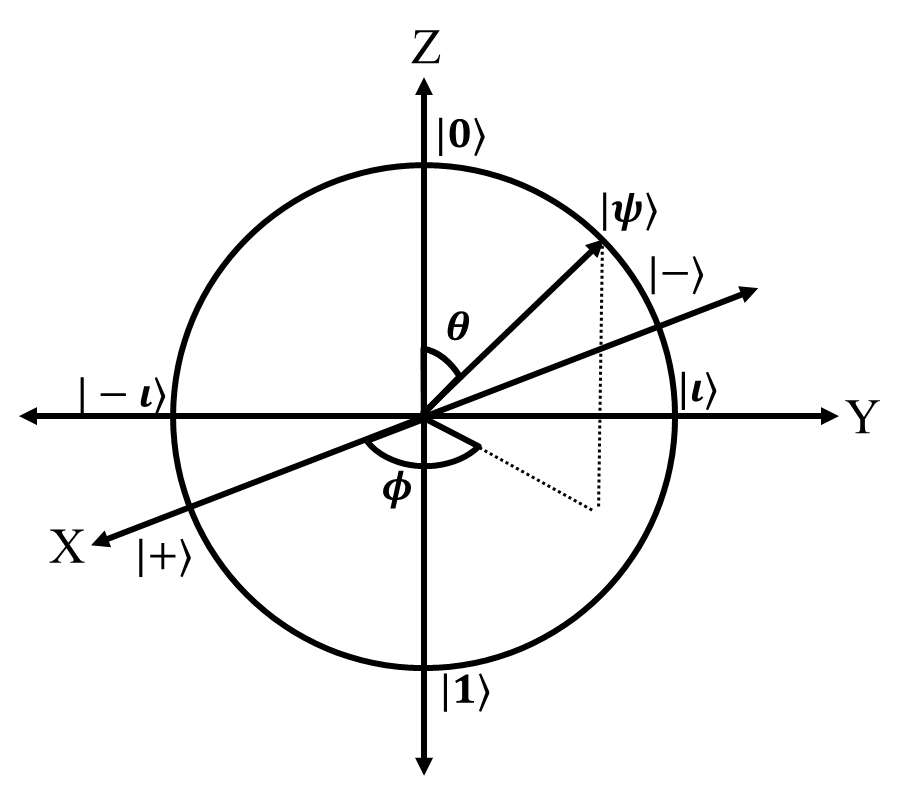
\includegraphics[width=0.6\textwidth]{../images/bloch_sphere_dia.png}
    \caption{Bloch-Poincare Sphere}
    \label{fig:bloch_sphere}
\end{figure}

Thus for different values of $\theta$ and $\phi$ we get different points on the bloch sphere which
represents the different states of a qubit. For a unique mapping from the $\theta$ and $\phi$ to the points on the Bloch Sphere,
we restrict the value of $\theta \in [0,\pi]$ and $\phi \in [0,2\pi]$. 
Thus, the state of a qubit can be represented as:
\[
    \ket{\psi}=\cos\left(\frac{\theta}{2}\right)\ket{0}+e^{\iota \phi}\sin\left(\frac{\theta}{2}\right)\ket{1}
\]
where $\theta \in [0,\pi]$ and $\phi \in [0,2\pi]$ are the polar (represents magnitude or argument) and azimuthal (represents relative phase) angles of the Bloch Sphere respectively.
The following code using Qiskit can be used to plot the Bloch Sphere.
For running the code you need to install the qiskit library. 
%Insert a link 
\href{https://docs.quantum.ibm.com/start/install}{Click here for guide on installing qiskit}
\begin{lstlisting}[language=Python]
import matplotlib.pyplot as plt
from qiskit.visualization import plot_bloch_vector # Import the function to plot the Bloch vector
from qiskit.visualization import plot_bloch_multivector # Import the function to plot the Bloch vector

'''
Function to plot the Bloch Sphere

plot_bloch_vector(bloch, title='', ax=None, figsize=None, coord_type='spherical', font_size=None)

Plots a Bloch Sphere

Parameters
- bloch (list[double]) - array of three elements where [<x>, <y>, <z>] (Cartesian) or 
[<r>, <theta>, <phi>] (spherical in radians) <theta> is inclination angle from +z direction 
<phi> is azimuth from +x direction
- title (str) - a string that represents the title of the plot
- ax (matplotlib.axes.Axes) - an axes of the current figure to plot the Bloch sphere into
- figsize (tuple) - a tuple (width, height) in inches that represents the size of the figure
- coord_type (str) - the coordinate system to use. 'spherical' or 'cartesian', default is cartesian
- font_size (int) - the font size of the tex

Returns
- matplotlib.figure.Figure - a matplotlib figure object

Raises
- ImportError - if matplotlib is not installed
'''

plot_bloch_vector([0,1,0],title='Bloch Sphere')
\end{lstlisting}
The output of the above code is shown in the figure \ref{fig:bloch_sphere_code}.
%Insert a figure
\begin{figure}[H]
    \centering
    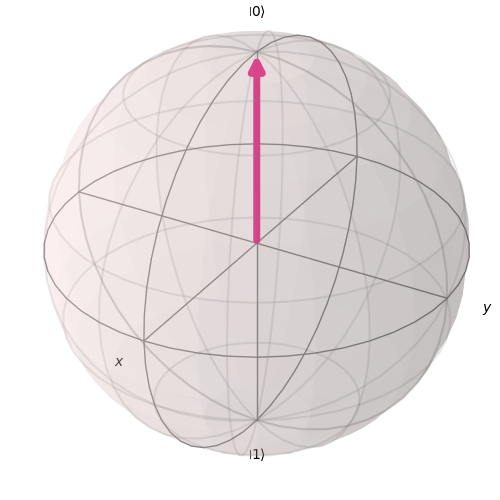
\includegraphics[width=0.5\textwidth]{../images/bloch_sphere.png}
    \caption{Bloch Sphere}
    \label{fig:bloch_sphere_code}
\end{figure}
\textbf{Note that the Bloch Sphere is a geometric representation of the pure states of a qubit. The mixed states of a qubit are represented by the interior of the Bloch Sphere.}

\begin{example}
    The state of a qubit for different values of $\theta$ and $\phi$ is shown in the table \ref{tab:bloch_sphere}.
    \begin{table}[H]
        \centering
        \begin{tabular}{|c|c|>{\centering\arraybackslash}m{8cm}|c|}
            \hline
            $\theta$ & $\phi$ & State of Qubit & At Axis\\
            \hline
            0 & 0 & $\ket{0}$ & +ve Z\\
            $\pi$ & 0 & $\ket{1}$ & -ve Z \\
            $\frac{\pi}{2}$ & 0 & $\ket{+} = \frac{1}{\sqrt{2}}(\ket{0} + \ket{1})$ & +ve X\\
            $\frac{\pi}{2}$ & $\pi$ & $\ket{-} = \frac{1}{\sqrt{2}}(\ket{0} - \ket{1})$ & -ve X\\
            $\frac{\pi}{2}$ & $\frac{\pi}{2}$ & $\ket{+\iota}=\frac{1}{\sqrt{2}}(\ket{0} + i\ket{1})$ & +ve Y \\
            $\frac{\pi}{2}$ & $-\frac{\pi}{2}$ & $\ket{-\iota}=\frac{1}{\sqrt{2}}(\ket{0} - i\ket{1})$ & -ve Y\\
            \hline
        \end{tabular}
        \caption{State of a Qubit for different values of $\theta$ and $\phi$}
        \label{tab:bloch_sphere}
    \end{table}
\end{example}

\textbf{Quantum Gates acting on Qubits can be thought of as rotations on the Bloch Sphere.}
This will be explained further in the later sections.

Note that orthonormal states reside at the ends of the diameter of the Bloch Sphere. 
Let a state $\ket{\psi}$ be represented by a point on the Bloch Sphere. The state $\ket{\psi}$ can be written as:
\[
    \ket{\psi}=\cos\left(\frac{\theta}{2}\right)\ket{0}+e^{\iota \phi}\sin\left(\frac{\theta}{2}\right)\ket{1}
\]
Then the state (say $\ket{\psi'}$) exactly opposite on the Bloch sphere will have the state:
\[
    \ket{\psi'}=\cos\left(\frac{\pi+\theta}{2}\right)\ket{0}+e^{\iota \phi}\sin\left(\frac{\pi+\theta}{2}\right)\ket{1}
\]
Thus, upon simplifying we get:
\[
    \ket{\psi'}=\cos\left(\frac{\pi+\theta}{2}\right)\ket{0}+e^{\iota \phi}\sin\left(\frac{\pi+\theta}{2}\right)\ket{1}
\]
\[
    \ket{\psi'}=-\sin \left(\frac{\theta}{2}\right)\ket{0}+e^{\iota \phi}\cos\left(\frac{\theta}{2}\right)\ket{1}
\]
Now taking the inner product of the states $\ket{\psi}$ and $\ket{\psi'}$ we get:
\[
    \braket{\psi|\psi'}=-\sin\left(\frac{\theta}{2}\right)\cos\left(\frac{\theta}{2}\right)+e^{\iota \phi}e^{-\iota \phi}\sin\left(\frac{\theta}{2}\right)\cos\left(\frac{\theta}{2}\right)=0
\]
Thus, the inner product is zero which implies that the states on the opposite ends of the Bloch Sphere are orthogonal.

\textbf{Note: Such a correspondence does not exist for higher dimensions i.e. No such visualization exists for say Qudits which is d level quantum systems.}
From figure \ref{fig:bloch_sphere} we can see that to convert from polar to cartesian coordinates we use the following relations:
\[
    x=r\sin\theta\cos\phi
\]
\[
    y=r\sin\theta\sin\phi
\]
\[
    z=r\cos\theta
\]
note that here $r=1$ (from pure states i.e. points on the surface of the sphere). To convert from carteisan to polar coordinates we use the following relations:
\[
    r=\sqrt{x^2+y^2+z^2}
\]
\[
    \theta=\cos^{-1}(z)
\]
\[
    \phi=\tan^{-1}\left(\frac{y}{x}\right)
\]
Let us denote the vector as $\vec{n}=(\sin\theta \cos \phi, \sin \theta \sin \phi, \cos \theta, \cos \theta)$.
Points on a Bloch sphere is alwyas a pure state.


\section{Single Qubit Gates}
As said earlier that quantum gates are unitary operators that act on the state of a quantum system. 
Recall from Appendix that the unitary operators are the ones that preserve the inner product of the vectors and the norm of the vectors i.e. they 
only rotate the vectors in the complex vector space (Rotation matrices in $\mathbb{C}^n$). Thus, a state normalized initially remains in the normalized state and does not change its norm 
upon the action of Unitary gates/operators.
The single qubit gates are the quantum gates that act on a single qubit, represented by 2x2 matrices. Since a quantum state is represented by a column vector (in some basis, generally standard basis). 
A gate is a unitary matrix/transformation 
that acts on the qubit(column vector) and changes its state to some other state.
They are rotations on the Bloch Sphere.
\begin{example}
    Consider a $2 \times 2$ matrix $U$ given as:
    \[
        U=\begin{bmatrix}
            a & b \\
            c & d
        \end{bmatrix}
    \]
    in the orthonormal input and output basis $\{\ket{0},\ket{1}\}$, thus, we can write the matrix $U$ as:
    \[
        U=a\ket{0}\bra{0}+b\ket{0}\bra{1}+c\ket{1}\bra{0}+d\ket{1}\bra{1}
    \]
    This, will be used to express the Pauli Matrices in the later sections.
\end{example}

\subsection{Pauli Matrices}
\subsubsection{Pauli-I Gate}
It is used for the measurement of decoherence (Qubits start to lose its Quantum abilities after certain time).
The Truth table is given as in table \ref{tab:pauli-i}. It does no rotation of the bloch vector on the Bloch Sphere.
%Insert a table
\begin{table}[H]
    \centering
    \begin{tabular}{|c|c|}
        \hline
        Input & Output\\
        \hline  
        $\ket{0}$ & $\ket{0}$\\
        $\ket{1}$ & $\ket{1}$\\
        \hline
    \end{tabular}
    \caption{Truth Table for Pauli-I Gate}
    \label{tab:pauli-i}
\end{table}
The code for the Pauli-I Gate is as follows:
\begin{lstlisting}[language=Python]
from qiskit import QuantumRegister, ClassicalRegister, QuantumCircuit
from numpy import pi

qreg_q = QuantumRegister(1, 'q')

circuit = QuantumCircuit(qreg_q)

circuit.id(qreg_q[0]) #For Pauli-Identity Gate
circuit.draw(output='mpl')#.savefig('../images/pauli-i.png') #Draw the circuit
\end{lstlisting}
The circuit symbol is as shown in figure \ref{fig:pauli-i}
\begin{figure}[H]
    \centering
    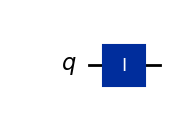
\includegraphics[width=0.3\textwidth]{../images/pauli-i.png}
    \caption{Pauli-I Gate}
    \label{fig:pauli-i}
\end{figure}
In operator Notation it is:
\begin{align*}
    I\ket{0}&=\ket{0} \\
    I\ket{1}&=\ket{1}
\end{align*}
It is represented by the matrix in the computational basis ($\ket{0},\ket{1}$) as:
\[
    \sigma_I=I=\begin{bmatrix}
        1 & 0 \\
        0 & 1
    \end{bmatrix}
\]
It's Eigen values are 1 and 1. It's Eigen vectors are any vector in the 2-D Space.
Note that it's Unitary($II^{\dagger}=I^{\dagger}I=I;I=I^{-1}$) and Hermitian Matrix($I=I^{\dagger}$), thus a Normal Matrix ($II^{\dagger}=I^{\dagger}I$) hence Unitarily digonalizable.
Thus, it has a Spectral decomposition (outer product representation) which can be written as:
\[
    I=\ket{0}\bra{0}+\ket{1}\bra{1}
\]
Action of Pauli-I Gate on a general qubit $\alpha\ket{0}+\beta\ket{1}$ is:
\[
    \begin{bmatrix}
        1 & 0 \\
        0 & 1
    \end{bmatrix}\begin{bmatrix}
        \alpha \\
        \beta
    \end{bmatrix}=\begin{bmatrix}
        \alpha \\
        \beta
    \end{bmatrix}= \alpha\ket{0}+\beta\ket{1}
\]

\subsubsection{Pauli-X Gate}
It is also known as the NOT gate. It is equivalent of Classical NOT Gate.
It is thus called Bit Flip Gate. The truth table is as in \ref{tab:pauli-x}. It does anticlockwise $\pi$ rotation about X 
axis of Bloch sphere. It flips the state $\ket{0}$ to $\ket{1}$ and $\ket{1}$ to $\ket{0}$.
\begin{table}[H]
    \centering
    \begin{tabular}{|c|c|}
        \hline
        Input & Output\\
        \hline
        $\ket{0}$ & $\ket{1}$\\
        $\ket{1}$ & $\ket{0}$\\
        \hline
    \end{tabular}
    \caption{Truth Table for Pauli-X Gate}
    \label{tab:pauli-x}
\end{table}

The code for the Pauli-X Gate is as follows:
\begin{lstlisting}[language=Python]
from qiskit import QuantumRegister, ClassicalRegister, QuantumCircuit
from numpy import pi

qreg_q = QuantumRegister(1, 'q')
circuit = QuantumCircuit(qreg_q,name='Not Gate')

circuit.x(qreg_q[0])

circuit.draw(output='mpl')#.savefig('../images/pauli-x.png') #Draw the circuit
\end{lstlisting}
The circuit symbol is as shown in figure \ref{fig:pauli-x}.
\begin{figure}[H]
    \centering
    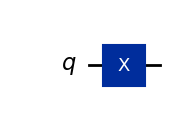
\includegraphics[width=0.3\textwidth]{../images/pauli-x.png}
    \caption{Pauli-X Gate}
    \label{fig:pauli-x}
\end{figure}
In the operator Notation it is:
\begin{align*}
    X\ket{0}&=\ket{1} \\
    X\ket{1}&=\ket{0}
\end{align*}
It is represented by the matrix in the computational basis ($\ket{0},\ket{1}$) as:
\[
    \sigma_X=X=\begin{bmatrix}
        0 & 1 \\
        1 & 0
    \end{bmatrix}
\]
It's Eigen values are 1 and -1. It's corresponding Eigen vectors are $\ket{+}=\frac{1}{\sqrt{2}}(\ket{0}+\ket{1})$ and $\ket{-}=\frac{1}{\sqrt{2}}(\ket{0}-\ket{1})$.
It is a Unitary and Hermitian Matrix. It is a Normal Matrix hence Unitarily Diagonalizable.
It has a Spectral decomposition (outer product representation) which can be written as:
\[
    X=\ket{+}\bra{+}-\ket{-}\bra{-}
\]
Upon, substituting the values of $\ket{+}$ and $\ket{-}$ we get:
\begin{align*}
    X&=\dfrac{1}{\sqrt{2}}(\ket{0}+\ket{1})\dfrac{1}{\sqrt{2}}(\bra{0}+\bra{1})-\dfrac{1}{\sqrt{2}}(\ket{0}-\ket{1})\dfrac{1}{\sqrt{2}}(\bra{0}-\bra{1})\\
    &=\dfrac{1}{2}(\ket{0}\bra{0}+\ket{0}\bra{1}+\ket{1}\bra{0}+\ket{1}\bra{1})+\dfrac{1}{2}(\ket{0}\bra{0}-\ket{0}\bra{1}-\ket{1}\bra{0}+\ket{1}\bra{1})\\
    &=\ket{0}\bra{1}+\ket{1}\bra{0}
\end{align*}
Thus, the Pauli-X Gate can also be written as:
\[
    X=\ket{0}\bra{1}+\ket{1}\bra{0}
\]
\textbf{Note that the Pauli-X Gate can be written as $X=HZH$ or $\sigma_X=H\sigma_Z H$  where $H$ and $Z$ are the Hadamard and Pauli-Z Gates respectively.}
Action of Pauli-X Gate on a general qubit $\ket{\psi}=\alpha\ket{0}+\beta\ket{1}$ is: 
\[
    \begin{bmatrix}
        0 & 1 \\
        1 & 0
    \end{bmatrix}\begin{bmatrix}
        \alpha \\
        \beta
    \end{bmatrix}=\begin{bmatrix}
        \beta \\
        \alpha
    \end{bmatrix}= \beta\ket{0}+\alpha\ket{1}
\]

\subsubsection{Pauli-Y Gate}
It is a anitclockwise $\pi$ rotation about Y axis of Bloch Sphere. 
It flips the Qubit and muultiplies a complex amplitude. The truth table is as in table \ref{tab:pauli-y}.
\begin{table}[H]
    \centering
    \begin{tabular}{|c|c|}
        \hline
        Input & Output\\
        \hline
        $\ket{0}$ & $i\ket{1}$\\
        $\ket{1}$ & $-i\ket{0}$\\
        \hline
    \end{tabular}
    \caption{Truth Table for Pauli-Y Gate}
    \label{tab:pauli-y}
\end{table}
The code for the Pauli-Y Gate is as follows:
\begin{lstlisting}[language=Python]
from qiskit import QuantumRegister, ClassicalRegister, QuantumCircuit
from numpy import pi

qreg_q = QuantumRegister(1, 'q')
circuit = QuantumCircuit(qreg_q,name='Not Gate')

circuit.y(qreg_q[0]) #Apply the Y gate

circuit.draw(output='mpl')#.savefig('../images/pauli-x.png') #Draw the circuit
\end{lstlisting}

The circuit symbol is as shown in figure \ref{fig:pauli-y}.
\begin{figure}[H]
    \centering
    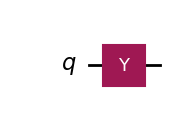
\includegraphics[width=0.3\textwidth]{../images/pauli-y.png}
    \caption{Pauli-Y Gate}
    \label{fig:pauli-y}
\end{figure}
In the operator Notation it is:
\begin{align*}
    Y\ket{0}&=i\ket{1} \\
    Y\ket{1}&=-i\ket{0}
\end{align*}
It is represented by the matrix in the computational basis ($\ket{0},\ket{1}$) as:
\[
    \sigma_Y=Y=\begin{bmatrix}
        0 & -i \\
        i & 0
    \end{bmatrix}
\]
It's Eigen values are 1 and -1. It's corresponding Eigen vectors are $\ket{+i}=\frac{1}{\sqrt{2}}(\ket{0}+i\ket{1})$ and $\ket{-i}=\frac{1}{\sqrt{2}}(\ket{0}-i\ket{1})$.
It is a Unitary and Hermitian Matrix. It is a Normal Matrix hence Unitarily Diagonalizable.
It has a Spectral decomposition (outer product representation) which can be written as:
\[
    Y=\ket{+i}\bra{+i}-\ket{-i}\bra{-i}
\]
Upon, substituting the values of $\ket{+i}$ and $\ket{-i}$ we get:
\begin{align*}
    Y&=\dfrac{1}{\sqrt{2}}(\ket{0}+i\ket{1})\dfrac{1}{\sqrt{2}}(\bra{0}-i\bra{1})-\dfrac{1}{\sqrt{2}}(\ket{0}-i\ket{1})\dfrac{1}{\sqrt{2}}(\bra{0}+i\bra{1})\\
    &=\dfrac{1}{2}(\ket{0}\bra{0}+i\ket{0}\bra{1}-i\ket{1}\bra{0}+i\ket{1}\bra{1})-\dfrac{1}{2}(\ket{0}\bra{0}-i\ket{0}\bra{1}+i\ket{1}\bra{0}+i\ket{1}\bra{1})\\
    &=i\ket{0}\bra{1}-i\ket{1}\bra{0}
\end{align*}
Thus, the Pauli-Y Gate can also be written as:
\[
    Y=-i\ket{0}\bra{1}+i\ket{1}\bra{0}
\]
\textbf{Note that the Pauli-Y Gate can be written as $Y=\iota XZ$ or $\sigma_Y=\iota \sigma_X\sigma_Z$  where $X$ and $Z$ are the Pauli-X and Pauli-Z Gates respectively.}
This means that the Pauli-Y Gate is a rotation about the Y-axis of the Bloch Sphere by $\pi$ in anticlocwise direction and is equivalent to a rotation about the X-axis by anticlockwise $\pi$ followed by a rotation about the Z-axis by anticlockwise $\pi$
(upto a global phase).

Action of Pauli-Y Gate on a general qubit $\ket{\psi}=\alpha\ket{0}+\beta\ket{1}$ is:
\[
    \begin{bmatrix}
        0 & -i \\
        i & 0
    \end{bmatrix}\begin{bmatrix}
        \alpha \\
        \beta
    \end{bmatrix}=\begin{bmatrix}
        -i\beta \\
        i\alpha
    \end{bmatrix}=i\alpha\ket{1}-i\beta\ket{0}
\]

\subsubsection{Pauli-Z Gate}
It is a anticlockwise $\pi$ rotation about Z axis of Bloch Sphere.
It flips the sign of the $\ket{1}$ state. It is also called Phase Flip/Phase shoft/Sign flip gate.
The truth table is as in table \ref{tab:pauli-z}.
\begin{table}[H]
    \centering
    \begin{tabular}{|c|c|}
        \hline
        Input & Output\\
        \hline
        $\ket{0}$ & $\ket{0}$\\
        $\ket{1}$ & $-\ket{1}$\\
        \hline
    \end{tabular}
    \caption{Truth Table for Pauli-Z Gate}
    \label{tab:pauli-z}
\end{table}
The code for the Pauli-Z Gate is as follows:
\begin{lstlisting}[language=Python]
from qiskit import QuantumRegister, ClassicalRegister, QuantumCircuit
from numpy import pi

qreg_q = QuantumRegister(1, 'q')
circuit = QuantumCircuit(qreg_q,name='Not Gate')

circuit.z(qreg_q[0]) #Apply the Z gate

circuit.draw(output='mpl')#.savefig('../images/pauli-z.png') #Draw the circuit
\end{lstlisting}
The circuit symbol is as shown in figure \ref{fig:pauli-z}.
\begin{figure}[H]
    \centering
    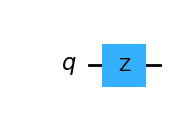
\includegraphics[width=0.3\textwidth]{../images/pauli-z.png}
    \caption{Pauli-Z Gate}
    \label{fig:pauli-z}
\end{figure}
In the operator Notation it is:
\begin{align*}
    Z\ket{0}&=\ket{0} \\
    Z\ket{1}&=-\ket{1}
\end{align*}
It is represented by the matrix in the computational basis ($\ket{0},\ket{1}$) as:
\[
    \sigma_Z=Z=\begin{bmatrix}
        1 & 0 \\
        0 & -1
    \end{bmatrix}
\]
It's Eigen values are 1 and -1. It's corresponding Eigen vectors are $\ket{0}$ and $\ket{1}$.
It is a Unitary and Hermitian Matrix. It is a Normal Matrix hence Unitarily Diagonalizable.
It has a Spectral decomposition (outer product representation) which can be written as:
\[
    Z=\ket{0}\bra{0}-\ket{1}\bra{1}
\]
In Compact form, we can write Pauli-Z Gate as:
\[
    Z\ket{j}=(-1)^j\ket{j}
\]
where $j=0,1$.
Action of Pauli-Z Gate on a general qubit $\ket{\psi}=\alpha\ket{0}+\beta\ket{1}$ is:
\[
    \begin{bmatrix}
        1 & 0 \\
        0 & -1
    \end{bmatrix}\begin{bmatrix}
        \alpha \\
        \beta
    \end{bmatrix}=\begin{bmatrix}
        \alpha \\
        -\beta
    \end{bmatrix}=\alpha\ket{0}-\beta\ket{1}
\]

\begin{importantnote}
Note that all the Pauli-gate are Unitary and Hermitian. Since, all the Unitary gates ($U^{\dagger}=U^{-1}$)
are reversible. Thus, from Postulate 2: Evolution, we can apply Pauli Gates. All the Pauli gates are reversible 
and thus can be applied in Quantum Circuits. The four Pauli gates can also be denoted as $X=\sigma_X$, $Y=\sigma_Y$, $Z=\sigma_Z$ and $I=\sigma_I$.
All the Pauli Gates as said earlier are anticlockwise rotations on the Bloch Sphere. The Pauli-X Gate is a $\pi$ rotation about the X-axis,
Pauli-Y Gate is a $\pi$ rotation about the Y-axis and Pauli-Z Gate is a $\pi$ rotation about the Z-axis. The Pauli-I Gate does not do any rotation on the Bloch Sphere.
Also note that applyin the same gate twice will be equivalent to applying the Identity Gate. Thus, the Pauli Gates are self-inverse. Since they are hermitian hence, $U^{\dagger}=U$ and 
they are unitary thus, $U^{\dagger}U=UU^{\dagger}=I$. Thus combining, the two we get $U^2=I$.
This, can also be verified as shown below:
\[
    X^2=\begin{bmatrix}
        0 & 1 \\
        1 & 0
    \end{bmatrix}\begin{bmatrix}
        0 & 1 \\
        1 & 0
    \end{bmatrix}=\begin{bmatrix}
        1 & 0 \\
        0 & 1
    \end{bmatrix}=I
\]
\[
    Y^2=\begin{bmatrix}
        0 & -i \\
        i & 0
    \end{bmatrix}\begin{bmatrix}
        0 & -i \\
        i & 0
    \end{bmatrix}=\begin{bmatrix}
        1 & 0 \\
        0 & 1
    \end{bmatrix}=I
\]
\[
    Z^2=\begin{bmatrix}
        1 & 0 \\
        0 & -1
    \end{bmatrix}\begin{bmatrix}
        1 & 0 \\
        0 & -1
    \end{bmatrix}=\begin{bmatrix}
        1 & 0 \\
        0 & 1
    \end{bmatrix}=I
\]
\[
    I^2=\begin{bmatrix}
        1 & 0 \\
        0 & 1
    \end{bmatrix}\begin{bmatrix}
        1 & 0 \\
        0 & 1
    \end{bmatrix}=\begin{bmatrix}
        1 & 0 \\
        0 & 1
    \end{bmatrix}=I
\]
Thus, we can see that all the Pauli Gates are self-inverse.
The Pauli gates also form the basis for the single qubit gates. Any single qubit gate can be written as a linear combination of the Pauli Gates.
In other words, any $2 \times 2$ matrix can be written as a linear combination of the Pauli Matrices.
\[
    A=\alpha I+\beta X+\gamma Y+\delta Z
\]
where $\alpha,\beta,\gamma,\delta$ are complex numbers. The Pauli Matrices, except Identity are also traceless (trace=0) and all the Pauli matrices are Hermitian.
Note here it should be presumed that the the rotations are always in anticlockwise direction.
\end{importantnote}

\subsection{Hadamard Gate}\label{qgate:hadamard}
It creates a superposition of Qubits. 
It is a $\pi$ rotation about the X+Z axis of Bloch Sphere or 
a $\pi/2$ rotation about the Y axis followed by a $\pi$ rotation about the X axis.
It is also called as the Square root of NOT gate. The truth table is as in table \ref{tab:hadamard}.
\begin{table}[H]
    \centering
    \begin{tabular}{|c|c|}
        \hline
        Input & Output\\
        \hline
        $\ket{0}$ & $\ket{+}=\frac{1}{\sqrt{2}}(\ket{0}+\ket{1})$\\
        $\ket{1}$ & $\ket{-}=\frac{1}{\sqrt{2}}(\ket{0}-\ket{1})$\\
        \hline
    \end{tabular}
    \caption{Truth Table for Hadamard Gate}
    \label{tab:hadamard}
\end{table}

The code for the Hadamard Gate is as follows:
\begin{lstlisting}[language=Python]
from qiskit import QuantumRegister, ClassicalRegister, QuantumCircuit
from numpy import pi

qreg_q = QuantumRegister(1, 'q')
circuit = QuantumCircuit(qreg_q,name='Hadamard Gate')

circuit.h(qreg_q[0]) #Apply the H gate

circuit.draw(output='mpl')#.savefig('../images/hadamard.png') #Draw the circuit
\end{lstlisting}

The circuit symbol is as shown in figure \ref{fig:hadamard}.
\begin{figure}[H]
    \centering
    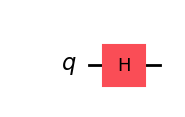
\includegraphics[width=0.3\textwidth]{../images/hadamard.png}
    \caption{Hadamard Gate}
    \label{fig:hadamard}
\end{figure}
In the operator Notation it is:
\begin{align*}
    H\ket{0}&=\dfrac{1}{\sqrt{2}}(\ket{0}+\ket{1})=\ket{+} \\
    H\ket{1}&=\dfrac{1}{\sqrt{2}}(\ket{0}-\ket{1})=\ket{-}
\end{align*}
Generally in a quantum circuit we intialise a qubit in state $\ket{0}$ and thus Hadamard gate can be used
to create a superposition. It is represented by the matrix in the computational basis ($\ket{0},\ket{1}$) as:
\[
    H=\dfrac{1}{\sqrt{2}}\begin{bmatrix}
        1 & 1 \\
        1 & -1
    \end{bmatrix}
\]
In compact form we can write the action of Hadamard Gate on one qubit as:
\[
    H\ket{j}=\dfrac{1}{\sqrt{2}}\sum_{k=0}^{1}(-1)^{jk}\ket{k}
\]
where $j=0,1$.
It is a Unitary and Hermitian Matrix. It is a Normal Matrix hence Unitarily Diagonalizable.
It has a Spectral decomposition (outer product representation) which can be written as:
\[
    H=\ket{+}\bra{0}+\ket{-}\bra{1}
\]
Action of Hadamard Gate on a general qubit $\ket{\psi}=\alpha\ket{0}+\beta\ket{1}$ is:
\[
    \dfrac{1}{\sqrt{2}}\begin{bmatrix}
        1 & 1 \\
        1 & -1
    \end{bmatrix}\begin{bmatrix}
        \alpha \\
        \beta
    \end{bmatrix}=\begin{bmatrix}
        \dfrac{\alpha+\beta}{\sqrt{2}} \\
        \dfrac{\alpha-\beta}{\sqrt{2}}
    \end{bmatrix}=\dfrac{\alpha+\beta}{\sqrt{2}}\ket{0}+\dfrac{\alpha-\beta}{\sqrt{2}}\ket{1}
\]
Note that the Hadamard gate is also a self-inverse gate. Since its Hermitian as well as Unitary, thus $H^{\dagger}=H$ and $H^{\dagger}H=HH^{\dagger}=I; H=H^{-1}$.
Thus, $H^2=I$. Intuitively this means that applying Hadamard gate twice will bring the quantum state back to the same quantum state. This can also be imagined 
as doing rotations on bloch sphere and then arriving back at the same state.
\[ H^2=\dfrac{1}{\sqrt{2}}\begin{bmatrix}
    1 & 1 \\
    1 & -1
\end{bmatrix}\dfrac{1}{\sqrt{2}}\begin{bmatrix}
    1 & 1 \\
    1 & -1
\end{bmatrix}=\dfrac{1}{2}\begin{bmatrix}
    1+1 & 1-1 \\
    1-1 & 1+1
\end{bmatrix}=\begin{bmatrix}
    1 & 0 \\
    0 & 1
\end{bmatrix}=I
\]
Thus, we can see that the Hadamard gate is self-inverse.
This means that if I apply Hadamard gate twice on $\ket{0}$ or on $\ket{1}$ then we will arrive back
at the same state. 
\[ H^2\ket{0}=H\ket{+}=\ket{0} \]
\[ H^2\ket{1}=H\ket{-}=\ket{1} \]

\textbf{Hadamard Gates on Multiple Qubits}\\
Hadamard gate can also be applied on multiple qubits. The Hadamard gate on multiple qubits (say n qubits) using tensor products is given as:
\[
    H^{\otimes n}=\underbrace{H\otimes H\otimes \ldots \otimes H}_{n \text{ times}}
\]
One of the way to find the Hadamard matrix is to perform the tensor product n times to get the Hadamard matrix acting on the n qubits. For example, we can find Hadamard gate acting on 2 qubits in matrix form using tensor product as:
\[
    H^{\otimes 2}=\dfrac{1}{\sqrt{2}}\begin{bmatrix}
        1 & 1 \\
        1 & -1
    \end{bmatrix}\otimes \dfrac{1}{\sqrt{2}}\begin{bmatrix}
        1 & 1 \\
        1 & -1
    \end{bmatrix}=\dfrac{1}{2}\begin{bmatrix}
        1 & 1 & 1 & 1 \\
        1 & -1 & 1 & -1 \\
        1 & 1 & -1 & -1 \\
        1 & -1 & -1 & 1
    \end{bmatrix}
\]
Clearly this does not scale.
Another method is, we can find the action of Hadamard gate on multiple qubits by applying the Hadamard gate on each qubit separately.
\[
    H^{\otimes n}(\ket{0}\otimes \ket{0}\otimes \ldots \otimes \ket{0})=H\ket{0}\otimes H\ket{0}\otimes \ldots \otimes H\ket{0}=\ket{+}\otimes \ket{+}\otimes \ldots \otimes \ket{+}
\]
This is a better method then writing entire matrix for n qubits. Thus, we can see that the Hadamard gate on multiple qubits creates a superposition of all possible states of n qubits.
So, for writing the Hadamard gate on multiple qubits, in a compact form, first we consider the compact form of $H^{\otimes 2}$ as:
\[
H^{\otimes 2}\ket{x}=H\ket{x_1}\otimes H\ket{x_2}
\] 
where $x=x_1x_2$. Now using the fact that $H\ket{x_1}=\dfrac{1}{\sqrt{2}}\sum_{y_1 \in \{0,1\}} (-1)^{x_1y_1}\ket{y_1}$ and $H\ket{x_2}=\dfrac{1}{\sqrt{2}}\sum_{y_2 \in \{0,1\}} (-1)^{x_2y_2}\ket{y_2}$, we get:
\[ 
H^{\otimes 2}\ket{x}=\dfrac{1}{2}\sum_{y_1,y_2 \in \{0,1\}} (-1)^{x_1y_1}(-1)^{x_2y_2}\ket{y_1}\otimes \ket{y_2}=\dfrac{1}{2}\sum_{y \in \{0,1\}^2}(-1)^{x\cdot y}\ket{y}
\]
where $x=x_1x_2$ and $y=y_1y_2$. Thus, it can be generalized and we can write the Hadamard gate on n qubits as:
\[
H^{\otimes n}\ket{x}=\dfrac{1}{\sqrt{2^n}}\sum_{y \in \{0,1\}^n}(-1)^{x\cdot y}\ket{y}
\]
where $x=x_1x_2\ldots x_n$ and $y=y_1y_2\ldots y_n$ and $x\cdot y$ is the dot product between $x$ and $y$. Thus, we can see that the Hadamard gate on n qubits creates a superposition of all possible states of n qubits.
In general, we start with state $\ket{0}$ for all the qubits initially, thus Action of hadamard gate on n qubits all in state $\ket{0}$ is:
\[
    H^{\otimes n}\ket{0}=\dfrac{1}{\sqrt{2^n}}\sum_{y \in \{0,1\}^n}\ket{y}
\]

\begin{example}
    \textbf{Fast Hadamard Gate using Tabular method :}\\
    Consider a state $\ket{\psi}=\dfrac{\ket{000}+\ket{110}-\ket{100}-\ket{111}}{\sqrt{4}}$. We are suppose to find
    $H^{\otimes 3}\ket{\psi}$. Thus, on solving using the equation for hadamard gate acting on multiple qubits $H^{\otimes n}\ket{x}=\dfrac{1}{\sqrt{2^n}}\sum_{y \in \{0,1\}^n}(-1)^{x\cdot y}\ket{y}$ 
    we get,
    \[
        \frac{1}{\sqrt{8}}\left(\ket{001}-\ket{011}+\ket{100}+\ket{110}+\ket{111}\right)
    \]
\end{example}




\subsection{$S$ and $S^{\dagger}$ Gate}
These are some specialised rotations,
\subsubsection{$S$ Gate}
It is $\pi/2$ rotation around Z axis of Bloch Sphere.
It is also called as the Phase Gate. The truth table is as in table \ref{tab:s}.
\begin{table}[H]
    \centering
    \begin{tabular}{|c|c|}
        \hline
        Input & Output\\
        \hline
        $\ket{0}$ & $\ket{0}$\\
        $\ket{1}$ & $i\ket{1}$\\
        \hline
    \end{tabular}
    \caption{Truth Table for S Gate}
    \label{tab:s}
\end{table}
The code for the S Gate is as follows:
\begin{lstlisting}[language=Python]
from qiskit import QuantumRegister, ClassicalRegister, QuantumCircuit
from numpy import pi

qreg_q = QuantumRegister(1, 'q')
circuit = QuantumCircuit(qreg_q,name='S Gate')

circuit.s(qreg_q[0]) #Apply the S gate

circuit.draw(output='mpl')#.savefig('../images/s-gate.png') #Draw the circuit
\end{lstlisting}

The circuit symbol is as shown in figure \ref{fig:s}.
\begin{figure}[H]
    \centering
    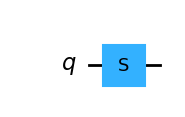
\includegraphics[width=0.3\textwidth]{../images/s-gate.png}
    \caption{S Gate}
    \label{fig:s}
\end{figure}
In the operator Notation it is:
\begin{align*}
    S\ket{0}&=\ket{0} \\
    S\ket{1}&=i\ket{1}
\end{align*}
It is represented by the matrix in the computational basis ($\ket{0},\ket{1}$) as:
\[
    S=\begin{bmatrix}
        1 & 0 \\
        0 & i
    \end{bmatrix}=e^{i\pi/4}\begin{bmatrix}
        e^{-i\pi/4} & 0 \\
        0 & e^{i\pi/4}
    \end{bmatrix}
\]
Thus, it is called as $\pi/4$ gate.
It's Eigen values are 1 and $i$. It's corresponding Eigen vectors are $\ket{0}$ and $\ket{1}$.
It is a Unitary and Hermitian Matrix. It is a Normal Matrix hence Unitarily Diagonalizable.
It has a Spectral decomposition (outer product representation) which can be written as:
\[
    S=\ket{0}\bra{0}+i\ket{1}\bra{1}
\]
Action of S Gate on a general qubit $\ket{\psi}=\alpha\ket{0}+\beta\ket{1}$ is:
\[
    \begin{bmatrix}
        1 & 0 \\
        0 & i
    \end{bmatrix}\begin{bmatrix}
        \alpha \\
        \beta
    \end{bmatrix}=\begin{bmatrix}
        \alpha \\
        i\beta
    \end{bmatrix}=\alpha\ket{0}+i\beta\ket{1}
\]


\subsubsection{$S^{\dagger}$ Gate}
It is $\pi/2$ rotation around Z axis of Bloch Sphere in the opposite direction.
It is also
called as the Conjugate Phase Gate. The truth table is as in table \ref{tab:s-dagger}.
\begin{table}[H]
    \centering
    \begin{tabular}{|c|c|}
        \hline
        Input & Output\\
        \hline
        $\ket{0}$ & $\ket{0}$\\
        $\ket{1}$ & $-i\ket{1}$\\
        \hline
    \end{tabular}
    \caption{Truth Table for $S^{\dagger}$ Gate}
    \label{tab:s-dagger}
\end{table}
The code for the $S^{\dagger}$ Gate is as follows:
\begin{lstlisting}[language=Python]
from qiskit import QuantumRegister, ClassicalRegister, QuantumCircuit
from numpy import pi

qreg_q = QuantumRegister(1, 'q')
circuit = QuantumCircuit(qreg_q,name='T Gate')

circuit.sdg(qreg_q[0]) #Apply the sdag gate

circuit.draw(output='mpl')#.savefig('../images/sdag-gate.png') #Draw the circuit
\end{lstlisting}

The circuit symbol is as shown in figure \ref{fig:s-dagger}.
\begin{figure}[H]
    \centering
    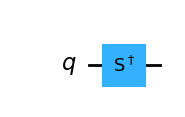
\includegraphics[width=0.3\textwidth]{../images/sdag-gate.png}
    \caption{$S^{\dagger}$ Gate}
    \label{fig:s-dagger}
\end{figure}
In the operator Notation it is:
\begin{align*}
    S^{\dagger}\ket{0}&=\ket{0} \\
    S^{\dagger}\ket{1}&=-i\ket{1}
\end{align*}

It is represented by the matrix in the computational basis ($\ket{0},\ket{1}$) as:
\[
    S^{\dagger}=\begin{bmatrix}
        1 & 0 \\
        0 & -i
    \end{bmatrix}=e^{-i\pi/4}\begin{bmatrix}
        e^{i\pi/4} & 0 \\
        0 & e^{-i\pi/4}
    \end{bmatrix}
\]
It's Eigen values are 1 and $-i$. It's corresponding Eigen vectors are $\ket{0}$ and $\ket{1}$.
It is a Unitary and Hermitian Matrix. It is a Normal Matrix hence Unitarily Diagonalizable.
It has a Spectral decomposition (outer product representation) which can be written as:
\[
    S^{\dagger}=\ket{0}\bra{0}-i\ket{1}\bra{1}
\]
Action of $S^{\dagger}$ Gate on a general qubit $\ket{\psi}=\alpha\ket{0}+\beta\ket{1}$ is:
\[
    \begin{bmatrix}
        1 & 0 \\
        0 & -i
    \end{bmatrix}\begin{bmatrix}
        \alpha \\
        \beta
    \end{bmatrix}=\begin{bmatrix}
        \alpha \\
        -i\beta
    \end{bmatrix}=\alpha\ket{0}-i\beta\ket{1}
\]
\textbf{Note that both $S$ and $S^{\dagger}$ gates are Unitary but not Hermitian thus they are not self-inverse. Reccall, that 
the only criteria for a gate is to be a Unitary (from Postulate 2: Unitary evolution) gate and not necessarily Hermitian.}

\subsection{$T$ and $T^{\dagger}$ Gate}
These are some specialised rotations,
\subsubsection{$T$ Gate}
It is $\pi/4$ rotation around Z axis of Bloch Sphere.
It is also called as the $\pi/8$ Gate. The truth table is as in table \ref{tab:t}.
\begin{table}[H]
    \centering
    \begin{tabular}{|c|c|}
        \hline
        Input & Output\\
        \hline
        $\ket{0}$ & $\ket{0}$\\
        $\ket{1}$ & $e^{i\pi/4}\ket{1}$\\
        \hline
    \end{tabular}
    \caption{Truth Table for T Gate}
    \label{tab:t}
\end{table}

The code for the T Gate is as follows:
\begin{lstlisting}[language=Python]
from qiskit import QuantumRegister, ClassicalRegister, QuantumCircuit
from numpy import pi

qreg_q = QuantumRegister(1, 'q')
circuit = QuantumCircuit(qreg_q,name='T Gate')

circuit.sdg(qreg_q[0]) #Apply the T gate

circuit.draw(output='mpl')#.savefig('../images/sdag-gate.png') #Draw the circuit    
\end{lstlisting}

The circuit symbol is as shown in figure \ref{fig:t}.
\begin{figure}[H]
    \centering
    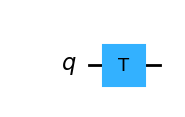
\includegraphics[width=0.3\textwidth]{../images/t-gate.png}
    \caption{T Gate}
    \label{fig:t}
\end{figure}

In the operator Notation it is:
\begin{align*}
    T\ket{0}&=\ket{0} \\
    T\ket{1}&=e^{i\pi/4}\ket{1}
\end{align*}
It is represented by the matrix in the computational basis ($\ket{0},\ket{1}$) as:
\[
    T=\begin{bmatrix}
        1 & 0 \\
        0 & e^{i\pi/4}
    \end{bmatrix}=e^{i\pi/8}\begin{bmatrix}
        e^{-i\pi/8} & 0 \\
        0 & e^{i\pi/8}
    \end{bmatrix}
\]
Thus, it is called as $\pi/8$ gate.
It's Eigen values are 1 and $e^{i\pi/4}$. It's corresponding Eigen vectors are $\ket{0}$ and $\ket{1}$.
It is a Unitary and Hermitian Matrix. It is a Normal Matrix hence Unitarily Diagonalizable.
It has a Spectral decomposition (outer product representation) which can be written as:
\[
    T=\ket{0}\bra{0}+e^{i\pi/4}\ket{1}\bra{1}
\]
Action of T Gate on a general qubit $\ket{\psi}=\alpha\ket{0}+\beta\ket{1}$ is:
\[
    \begin{bmatrix}
        1 & 0 \\
        0 & e^{i\pi/4}
    \end{bmatrix}\begin{bmatrix}
        \alpha \\
        \beta
    \end{bmatrix}=\begin{bmatrix}
        \alpha \\
        e^{i\pi/4}\beta
    \end{bmatrix}=\alpha\ket{0}+e^{i\pi/4}\beta\ket{1}
\]

\subsubsection{$T^{\dagger}$ Gate}
It is $\pi/4$ rotation around Z axis of Bloch Sphere in the opposite direction.
It is also called as the $\pi/8$ Gate. The truth table is as in table \ref{tab:t-dagger}.
\begin{table}[H]
    \centering
    \begin{tabular}{|c|c|}
        \hline
        Input & Output\\
        \hline
        $\ket{0}$ & $\ket{0}$\\
        $\ket{1}$ & $e^{-i\pi/4}\ket{1}$\\
        \hline
    \end{tabular}
    \caption{Truth Table for $T^{\dagger}$ Gate}
    \label{tab:t-dagger}
\end{table}

The code for the $T^{\dagger}$ Gate is as follows:
\begin{lstlisting}[language=Python]
from qiskit import QuantumRegister, ClassicalRegister, QuantumCircuit
from numpy import pi

qreg_q = QuantumRegister(1, 'q')
circuit = QuantumCircuit(qreg_q,name='T Gate')

circuit.tdg(qreg_q[0]) #Apply the T gate

circuit.draw(output='mpl')#.savefig('../images/tdag-gate.png') #Draw the circuit
\end{lstlisting}

The circuit symbol is as shown in figure \ref{fig:t-dagger}.
\begin{figure}[H]
    \centering
    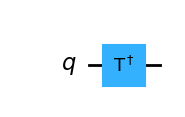
\includegraphics[width=0.3\textwidth]{../images/tdag-gate.png}
    \caption{$T^{\dagger}$ Gate}
    \label{fig:t-dagger}
\end{figure}

In the operator Notation it is:
\begin{align*}
    T^{\dagger}\ket{0}&=\ket{0} \\
    T^{\dagger}\ket{1}&=e^{-i\pi/4}\ket{1}
\end{align*}

It is represented by the matrix in the computational basis ($\ket{0},\ket{1}$) as:
\[
    T^{\dagger}=\begin{bmatrix}
        1 & 0 \\
        0 & e^{-i\pi/4}
    \end{bmatrix}=e^{-i\pi/8}\begin{bmatrix}
        e^{i\pi/8} & 0 \\
        0 & e^{-i\pi/8}
    \end{bmatrix}
\]
It's Eigen values are 1 and $e^{-i\pi/4}$. It's corresponding Eigen vectors are $\ket{0}$ and $\ket{1}$.
It is a Unitary and Hermitian Matrix. It is a Normal Matrix hence Unitarily Diagonalizable.
It has a Spectral decomposition (outer product representation) which can be written as:
\[
    T^{\dagger}=\ket{0}\bra{0}+e^{-i\pi/4}\ket{1}\bra{1}
\]
Action of $T^{\dagger}$ Gate on a general qubit $\ket{\psi}=\alpha\ket{0}+\beta\ket{1}$ is:
\[
    \begin{bmatrix}
        1 & 0 \\
        0 & e^{-i\pi/4}
    \end{bmatrix}\begin{bmatrix}
        \alpha \\
        \beta
    \end{bmatrix}=\begin{bmatrix}
        \alpha \\
        e^{-i\pi/4}\beta
    \end{bmatrix}=\alpha\ket{0}+e^{-i\pi/4}\beta\ket{1}
\]

Some relations between S and T Gates:
\begin{align*}
    S&=T^2 \\
    S^{\dagger}&=T^{\dagger}T^{\dagger}
\end{align*}
This can be verified as follows. Intuitively, one can think as twice $\pi/4$
rotation around Z axis is $\pi/2$ rotation around Z axis. Thus, the reltaions.
\begin{align*}
    T^2&=\begin{bmatrix}
        1 & 0 \\
        0 & e^{i\pi/4}
    \end{bmatrix}\begin{bmatrix}
        1 & 0 \\
        0 & e^{i\pi/4}
    \end{bmatrix}=\begin{bmatrix}
        1 & 0 \\
        0 & e^{i\pi/2}
    \end{bmatrix}=\begin{bmatrix}
        1 & 0 \\
        0 & i
    \end{bmatrix}=S \\
    T^{\dagger}T^{\dagger}&=\begin{bmatrix}
        1 & 0 \\
        0 & e^{-i\pi/4}
    \end{bmatrix}\begin{bmatrix}
        1 & 0 \\
        0 & e^{-i\pi/4}
    \end{bmatrix}=\begin{bmatrix}
        1 & 0 \\
        0 & e^{-i\pi/2}
    \end{bmatrix}=\begin{bmatrix}
        1 & 0 \\
        0 & -i
    \end{bmatrix}=S^{\dagger}
\end{align*}


\subsection{Quantum Rotation Gates}
These are generalized rotations  in the Bloch Sphere 
denoted as $R_X,R_Y,R_Z$ about the X,Y and Z axis of Bloch Sphere respectively.
\subsubsection{$R_X$ Gate}
It is a rotation about X axis of Bloch Sphere by an angle $\theta$. This is denoted
as $R^{X}_{\theta}$.
The matrix representation of $R^{X}_{\theta}$ is:
\[
    R^{X}_{\theta}=\begin{bmatrix}
        \cos(\theta/2) & -i\sin(\theta/2) \\
        -i\sin(\theta/2) & \cos(\theta/2)
    \end{bmatrix}=\cos \frac{\theta}{2}I-\iota \sin\frac{\theta}{2}\sigma_X=e^{-\iota\frac{\theta}{2}\sigma_X}
\]
The code for the $R_X$ Gate is as follows:
\begin{lstlisting}[language=Python]
from qiskit import QuantumRegister, ClassicalRegister, QuantumCircuit
from numpy import pi

qreg_q = QuantumRegister(1, 'q')
circuit = QuantumCircuit(qreg_q,name='U1 Gate')

circuit.rx(pi/2,qreg_q[0]) #Apply the RX gate

circuit.draw(output='mpl')#.savefig('../images/rx-gate.png') #Draw the circuit
\end{lstlisting}

The circuit symbol is as shown in figure \ref{fig:rx}.
\begin{figure}[H]
    \centering
    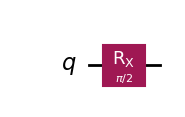
\includegraphics[width=0.3\textwidth]{../images/rx-gate.png}
    \caption{$R_X$ Gate}
    \label{fig:rx}
\end{figure}
Note that the value $\pi/2$ given in the figure \ref{fig:rx} denotes the angle by which we rotate around the X Axis of Bloch Sphere.

\subsubsection{$R_Y$ Gate}
It is a rotation about Y axis of Bloch Sphere by an angle $\theta$. This is denoted
as $R^{Y}_{\theta}$.
The matrix representation of $R^{Y}_{\theta}$ is:
\[
    R^{Y}_{\theta}=\begin{bmatrix}
        \cos(\theta/2) & -\sin(\theta/2) \\
        \sin(\theta/2) & \cos(\theta/2)
    \end{bmatrix}= \cos \frac{\theta}{2}I-\iota \cos \frac{\theta}{2}\sigma_Y=e^{-\iota \frac{\theta}{2}\sigma_Y}
\]
The code for the $R_Y$ Gate is as follows:
\begin{lstlisting}[language=Python]
from qiskit import QuantumRegister, ClassicalRegister, QuantumCircuit
from numpy import pi

qreg_q = QuantumRegister(1, 'q')
circuit = QuantumCircuit(qreg_q,name='RY Gate')

circuit.ry(pi/2,qreg_q[0]) #Apply the RY gate

circuit.draw(output='mpl')#.savefig('../images/ry-gate.png') #Draw the circuit
\end{lstlisting}

The circuit symbol is as shown in figure \ref{fig:ry}.
\begin{figure}[H]
    \centering
    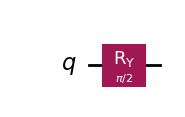
\includegraphics[width=0.3\textwidth]{../images/ry-gate.png}
    \caption{$R_Y$ Gate}
    \label{fig:ry}
\end{figure}
Note here the value $\pi/2$ denotes the angle by which we rotate around the Y Axis of Bloch Sphere.

\subsubsection{$R_Z$ Gate}
It is a rotation about Z axis of Bloch Sphere by an angle $\theta$. This is denoted
as $R^{Z}_{\theta}$.
The matrix representation of $R^{Z}_{\theta}$ is:
\[
    R^{Z}_{\theta}=\begin{bmatrix}
        e^{-i\theta/2} & 0 \\
        0 & e^{i\theta/2}
    \end{bmatrix}=\cos \frac{\theta}{2}I-\iota \cos \frac{\theta}{2}\sigma_Z=e^{-\iota \frac{\theta}{2}\sigma_Z}
\]

The code for the $R_Z$ Gate is as follows:
\begin{lstlisting}[language=Python]
from qiskit import QuantumRegister, ClassicalRegister, QuantumCircuit
from numpy import pi

qreg_q = QuantumRegister(1, 'q')
circuit = QuantumCircuit(qreg_q,name='RZ Gate')

circuit.rz(pi/2,qreg_q[0]) #Apply the RZ gate

circuit.draw(output='mpl')#.savefig('../images/rz-gate.png') #Draw the circuit
\end{lstlisting}

The circuit symbol is as shown in figure \ref{fig:rz}.
\begin{figure}[H]
    \centering
    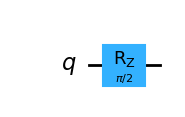
\includegraphics[width=0.3\textwidth]{../images/rz-gate.png}
    \caption{$R_Z$ Gate}
    \label{fig:rz}
\end{figure}
Note here the value $\pi/2$ denotes the angle by which we rotate around the Z Axis of Bloch Sphere.

This Quantum Rotation Gates can be used in making variational circuit as angles can vary.

\subsection{Universal Quantum Gates}
To construct any single qubit Quantum gates.
\[
    U_3(\theta,\phi,\lambda)=\begin{bmatrix}
        \cos(\theta/2) & -e^{i\lambda}\sin(\theta/2) \\
        e^{i\phi}\sin(\theta/2) & e^{i(\phi+\lambda)}\cos(\theta/2)
    \end{bmatrix}
\]
where $\theta,\phi,\lambda\in\mathbb{R}$ are rotations around x, y and z axis respectively.
Here, $0 \leq \theta \leq \pi$, $0\leq \phi \leq 2\pi$ and $0\leq \lambda \leq 2\pi$.
Similarly, we can fix $\theta$ and write $U_2$ gate as:
\[
    U_2(\phi,\lambda)=\begin{bmatrix}
        1 & -e^{i\lambda} \\
        e^{i\phi} & e^{i(\phi+\lambda)}
    \end{bmatrix}
\]
Here $\theta=\pi/2$ by default.
Similarly, we can fix $\theta$ and $\phi$ and write $U_1$ gate as:
\[
    U_1(\lambda)=\begin{bmatrix}
        1 & 0 \\
        0 & e^{i\lambda}
    \end{bmatrix}
\]
Here $\theta=\phi=0$ by default.

The code for the $U_3$ Gate is as follows:
\begin{lstlisting}[language=Python]
from qiskit import QuantumRegister, ClassicalRegister, QuantumCircuit
from numpy import pi

qreg_q = QuantumRegister(1, 'q')
circuit = QuantumCircuit(qreg_q,name='U3 Gate')

circuit.u(pi/2,pi/2,pi/2,qreg_q[0]) #Apply the U3 gate

circuit.draw(output='mpl')#.savefig('../images/u3-gate.png') #Draw the circuit
\end{lstlisting}

The circuit symbol is as shown in figure \ref{fig:u3}.
\begin{figure}[H]
    \centering
    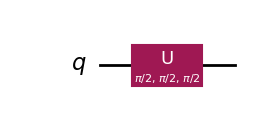
\includegraphics[width=0.3\textwidth]{../images/u3-gate.png}
    \caption{$U_3$ Gate}
    \label{fig:u3}
\end{figure}
Note here the values $\pi/2,\pi/2,\pi/2$ denotes the angles $\theta,\phi,\lambda$ by which we rotate around the Bloch Sphere respectively.

\section{Multi-Qubit Gates}
Quantum Pauli gates and hadmard gate are Unitary and Hermitian, and all the other single qubit gate are Unitary, hence, reversible.
In general, we can generalise any single qubit gate to multi-qubit gate.
Note that since all the gates can be in general represented as Unitary Matrices, thus the number of 
qubits in input = number of qubits in output always. Multi-Qubit gates act on multiple qubits at once thus the matrices are of
size $2^n \times 2^n$ where $n$ is the number of qubits.

\subsection{Two-qubit Gates}
\subsubsection{CNOT/CX Gate}
It is a two qubit gate, also called as the Controlled-NOT gate.
Here the 1st Qubit is controlled and the 2nd Qubit is target.
(It is also possible in the other way that the 2nd Qubit is controlled and the 1st Qubit is target).
This gate is used to create entanglement.
The truth table is as in table \ref{tab:cnot}.
\begin{table}[H]
    \centering
    \begin{tabular}{|c|c|c|}
        \hline
        Input & Output\\
        \hline
        $\ket{00}$ & $\ket{00}$\\
        $\ket{01}$   & $\ket{01}$\\
        $\ket{10}$   & $\ket{11}$\\
        $\ket{11}$  & $\ket{10}$\\
        \hline
    \end{tabular}
    \caption{Truth Table for CNOT Gate}
    \label{tab:cnot}
\end{table}
For the table in \ref{tab:cnot}, the 1st Qubit is control and the 2nd Qubit is target.
Thus, the CNOT gate flips the target qubit if the control qubit is $\ket{1}$.
The code for the CNOT Gate is as follows:
\begin{lstlisting}[language=Python]
from qiskit import QuantumRegister, ClassicalRegister, QuantumCircuit
from numpy import pi

# Add 2 qubits for CNOT gate demo
qreg_q = QuantumRegister(2, 'q')
circuit = QuantumCircuit(qreg_q,name='CNOT Gate')

circuit.cx(qreg_q[0],qreg_q[1]) #Apply the CNOT gate

circuit.draw(output='mpl')#.savefig('../images/cnot-gate.png') #Draw the circuit
\end{lstlisting}

The circuit symbol is as shown in figure \ref{fig:cnot}.
\begin{figure}[H]
    \centering
    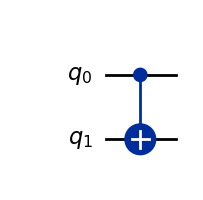
\includegraphics[width=0.3\textwidth]{../images/cnot-gate.png}
    \caption{CNOT Gate}
    \label{fig:cnot}
\end{figure}
Here it can be seen that the 1st Qubit is control and the 2nd Qubit is target. In the
figure \ref{fig:cnot}, the dot denotes the control qubit and the cross denotes the target qubit.

In the operator Notation it is:
\begin{align*}
    CX\ket{00}&=\ket{00} \\
    CX\ket{01}&=\ket{01} \\
    CX\ket{10}&=\ket{11} \\
    CX\ket{11}&=\ket{10}
\end{align*}
It is represented by the matrix in the computational basis ($\ket{00},\ket{01},\ket{10},\ket{11}$) as:
\[
    CX=\begin{bmatrix}
        1 & 0 & 0 & 0 \\
        0 & 1 & 0 & 0 \\
        0 & 0 & 0 & 1 \\
        0 & 0 & 1 & 0
    \end{bmatrix}
\]
In Outer product representation, it can be written as:
\[
    CX=\ket{00}\bra{00}+\ket{01}\bra{01}+\ket{10}\bra{11}+\ket{11}\bra{10}
\]
In Compact form we can write the CNOT gate as:
\[
    CX\ket{xy}=\ket{x(x\oplus y)}
\]
where $\oplus$ denotes the XOR operation. It is a non-linear operation. It is used in Quantum Error Correction Codes.
This is a very important gate which is used in Teleoprtation protocol, Superdense Coding, Quantum Error Correction Codes etc.
Action of CX/CNOT on general two - qubit $\ket{\psi} = \alpha\ket{00}+\beta\ket{01}+\gamma\ket{10}+\delta\ket{11}$ is:
\[
    \begin{bmatrix} 
        1 & 0 & 0 & 0 \\
        0 & 1 & 0 & 0 \\
        0 & 0 & 0 & 1 \\
        0 & 0 & 1 & 0
    \end{bmatrix}\begin{bmatrix}
        \alpha \\
        \beta \\
        \gamma \\
        \delta
    \end{bmatrix}=\begin{bmatrix}
        \alpha \\
        \beta \\
        \delta \\
        \gamma
    \end{bmatrix}=\alpha\ket{00}+\beta\ket{01}+\delta\ket{10}+\gamma\ket{11}
\]

\subsubsection{CY Gate}
It is a two qubit gate, also called as the Controlled-Y gate.
Here the 1st Qubit is controlled and the 2nd Qubit is target (Pauli - Y Gate)
(It is also possible in the other way that the 2nd Qubit is controlled and the 1st Qubit is target).

The truth table is as in table \ref{tab:cy}.
\begin{table}[H]
    \centering
    \begin{tabular}{|c|c|c|}
        \hline
        Input & Output\\
        \hline
        $\ket{00}$ & $\ket{00}$\\
        $\ket{01}$   & $\ket{01}$\\
        $\ket{10}$   & $i\ket{10}$\\
        $\ket{11}$  & $-i\ket{11}$\\
        \hline
    \end{tabular}
    \caption{Truth Table for CY Gate}
    \label{tab:cy}
\end{table}
For the table in \ref{tab:cy}, the 1st Qubit is control and the 2nd Qubit is target.
Thus, the CY gate flips the target qubit if the control qubit is $\ket{1}$.
The code for the CY Gate is as follows:
\begin{lstlisting}[language=Python]
from qiskit import QuantumRegister, ClassicalRegister, QuantumCircuit
from numpy import pi

# Add 2 qubits for CNOT gate demo
qreg_q = QuantumRegister(2, 'q')
circuit = QuantumCircuit(qreg_q,name='CY Gate')

circuit.cy(qreg_q[0],qreg_q[1]) #Apply the CY gate

circuit.draw(output='mpl')#.savefig('../images/cy-gate.png') #Draw the circuit
\end{lstlisting}

The circuit symbol is as shown in figure \ref{fig:cy}.
\begin{figure}[H]
    \centering
    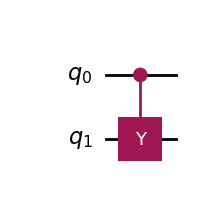
\includegraphics[width=0.3\textwidth]{../images/cy-gate.png}
    \caption{CY Gate}
    \label{fig:cy}
\end{figure}
In this figure \ref{fig:cy}, the first qubit is control and the second qubit is target.
If the first qubit is $\ket{1}$, then Y gate is applied on the second qubit. The Y Gate
is a gate which rotates the qubit by $\pi$ around the Y axis of Bloch Sphere. Thus, if
the input is $\ket{0}$, then the output is $\ket{0}$ and if the input is $\ket{1}$, then the output is $-i\ket{1}$.

In the operator Notation it is:
\begin{align*}
    CY\ket{00}&=\ket{00} \\
    CY\ket{01}&=\ket{01} \\
    CY\ket{10}&=i\ket{11} \\
    CY\ket{11}&=-i\ket{10}
\end{align*}
It is represented by the matrix in the computational basis ($\ket{00},\ket{01},\ket{10},\ket{11}$) as:
\[
    CY=\begin{bmatrix}
        1 & 0 & 0 & 0 \\
        0 & 1 & 0 & 0 \\
        0 & 0 & 0 & -\iota \\
        0 & 0 & \iota & 0
    \end{bmatrix}
\]
In Outer product representation, it can be written as:
\[
    CY=\ket{00}\bra{00}+\ket{01}\bra{01}+\iota\ket{11}\bra{10}-\iota\ket{10}\bra{11}
\]
In Compact form we can write the CY gate as:
\[
    CY\ket{xy}=(-1)^y\iota^x\ket{x(x\oplus y)}
\]
Flipping amplitude of 1 state. Marking of this state can be untilised for marking elements in data base.
It is useful in Grover's Algorithm.

Action of CY on general two - qubit $\ket{\psi} = \alpha\ket{00}+\beta\ket{01}+\gamma\ket{10}+\delta\ket{11}$ is:
\[
    \begin{bmatrix} 
        1 & 0 & 0 & 0 \\
        0 & 1 & 0 & 0 \\
        0 & 0 & 0 & -\iota \\
        0 & 0 & \iota & 0
    \end{bmatrix}\begin{bmatrix}
        \alpha \\
        \beta \\
        \gamma \\
        \delta
    \end{bmatrix}=\begin{bmatrix}
        \alpha \\
        \beta \\
        \iota\delta \\
        -\iota\gamma
    \end{bmatrix}=\alpha\ket{00}+\beta\ket{01}-\iota\delta\ket{10}+\iota\gamma\ket{11}
\]

\subsubsection{CZ/CPHASE Gate}
It is a two qubit gate, also called as the Controlled-Z gate.
Here the 1st Qubit is controlled and the 2nd Qubit is target (Pauli - Z Gate)
(It is also possible in the other way that the 2nd Qubit is controlled and the 1st Qubit is target).

The truth table is as in table \ref{tab:cz}.
\begin{table}[H]
    \centering
    \begin{tabular}{|c|c|c|}
        \hline
        Input & Output\\
        \hline
        $\ket{00}$ & $\ket{00}$\\
        $\ket{01}$   & $\ket{01}$\\
        $\ket{10}$   & $\ket{10}$\\
        $\ket{11}$  & $-\ket{11}$\\
        \hline
    \end{tabular}
    \caption{Truth Table for CZ Gate}
    \label{tab:cz}
\end{table}
For the table in \ref{tab:cz}, the 1st Qubit is control and the 2nd Qubit is target.
Thus, the CZ gate flips the target qubit if the control qubit is $\ket{1}$.
The code for the CZ Gate is as follows:
\begin{lstlisting}[language=Python]
from qiskit import QuantumRegister, ClassicalRegister, QuantumCircuit
from numpy import pi

qreg_q = QuantumRegister(2, 'q')
circuit = QuantumCircuit(qreg_q,name='CZ Gate')

circuit.cz(qreg_q[0],qreg_q[1]) #Apply the CZ gate

circuit.draw(output='mpl')#.savefig('../images/CZ-gate.png') #Draw the circuit
\end{lstlisting}

The circuit symbol is as shown in figure \ref{fig:cz}.
\begin{figure}[H]
    \centering
    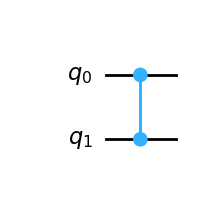
\includegraphics[width=0.3\textwidth]{../images/CZ-gate.png}
    \caption{CZ Gate}
    \label{fig:cz}
\end{figure}
In this figure \ref{fig:cz}, the first qubit is control and the second qubit is target.
If the first qubit is $\ket{1}$, then Z gate is applied on the second qubit. The Z Gate
is a gate which rotates the qubit by $\pi$ around the Z axis of Bloch Sphere. Thus, if 
the input is $\ket{0}$, then the output is $\ket{0}$ and if the input is $\ket{1}$, then the output is $-\ket{1}$.

In the operator Notation it is:
\begin{align*}
    CZ\ket{00}&=\ket{00} \\
    CZ\ket{01}&=\ket{01} \\
    CZ\ket{10}&=\ket{10} \\
    CZ\ket{11}&=-\ket{11}
\end{align*}
It is represented by the matrix in the computational basis ($\ket{00},\ket{01},\ket{10},\ket{11}$) as:
\[
    CZ=\begin{bmatrix}
        1 & 0 & 0 & 0 \\
        0 & 1 & 0 & 0 \\
        0 & 0 & 1 & 0 \\
        0 & 0 & 0 & -1
    \end{bmatrix}
\]
In Outer product representation, it can be written as:
\[
    CZ=\ket{00}\bra{00}+\ket{01}\bra{01}+\ket{10}\bra{10}-\ket{11}\bra{11}
\]
In Compact form we can write the CZ gate as:
\[
    CZ\ket{xy}=(-1)^{xy}\ket{xy}
\]

Action of CZ on general two - qubit $\ket{\psi} = \alpha\ket{00}+\beta\ket{01}+\gamma\ket{10}+\delta\ket{11}$ is:
\[
    \begin{bmatrix} 
        1 & 0 & 0 & 0 \\
        0 & 1 & 0 & 0 \\
        0 & 0 & 1 & 0 \\
        0 & 0 & 0 & -1
    \end{bmatrix}\begin{bmatrix}
        \alpha \\
        \beta \\
        \gamma \\
        \delta
    \end{bmatrix}=\begin{bmatrix}
        \alpha \\
        \beta \\
        \gamma \\
        -\delta
    \end{bmatrix}=\alpha\ket{00}+\beta\ket{01}+\gamma\ket{10}-\delta\ket{11}
\]

\subsubsection{CH/ Controlled Hadamard Gate}
It is a two qubit gate, also called as the Controlled-Hadamard gate.
Here the 1st Qubit is controlled and the 2nd Qubit is target.
The truth table is as in table \ref{tab:ch}.
\begin{table}[H]
    \centering
    \begin{tabular}{|c|c|c|}
        \hline
        Input & Output\\
        \hline
        $\ket{00}$ & $\ket{00}$\\
        $\ket{01}$   & $\ket{01}$\\
        $\ket{10}$   & $\frac{1}{\sqrt{2}}(\ket{10}+\ket{11})$\\
        $\ket{11}$  & $\frac{1}{\sqrt{2}}(\ket{10}-\ket{11})$\\
        \hline
    \end{tabular}
    \caption{Truth Table for CH Gate}
    \label{tab:ch}
\end{table}
For the table in \ref{tab:ch}, the 1st Qubit is control and the 2nd Qubit is target.
Thus, the CH gate applies Hadamard gate on the target qubit if the control qubit is $\ket{1}$.
The code for the CH Gate is as follows:
\begin{lstlisting}[language=Python]
from qiskit import QuantumRegister, ClassicalRegister, QuantumCircuit
from numpy import pi

# Add 2 qubits for CNOT gate demo
qreg_q = QuantumRegister(2, 'q')
circuit = QuantumCircuit(qreg_q,name='CY Gate')

circuit.ch(qreg_q[0],qreg_q[1]) #Apply the CH gate

circuit.draw(output='mpl')#.savefig('../images/ch-gate.png') #Draw the circuit
\end{lstlisting}

The circuit symbol is as shown in figure \ref{fig:ch}.
\begin{figure}[H]
    \centering
    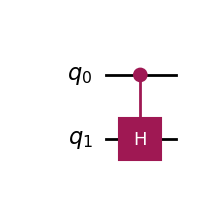
\includegraphics[width=0.3\textwidth]{../images/ch-gate.png}
    \caption{CH Gate}
    \label{fig:ch}
\end{figure}
In this figure \ref{fig:ch}, the first qubit is control and the second qubit is target.
If the first qubit is $\ket{1}$, then Hadamard gate is applied on the second qubit. The Hadamard Gate
is a gate which rotates the qubit by $\pi$ around the X axis of Bloch Sphere. Thus, if
the input is $\ket{0}$, then the output is $\ket{0}$ and if the input is $\ket{1}$, then the output is $\frac{1}{\sqrt{2}}(\ket{0}+\ket{1})$.

In the operator Notation it is:
\begin{align*}
    CH\ket{00}&=\ket{00} \\
    CH\ket{01}&=\ket{01} \\
    CH\ket{10}&=\frac{1}{\sqrt{2}}(\ket{10}+\ket{11}) \\
    CH\ket{11}&=\frac{1}{\sqrt{2}}(\ket{10}-\ket{11})
\end{align*}
It is represented by the matrix in the computational basis ($\ket{00},\ket{01},\ket{10},\ket{11}$) as:
\[
    CH=\begin{bmatrix}
        1 & 0 & 0 & 0 \\
        0 & 1 & 0 & 0 \\
        0 & 0 & \frac{1}{\sqrt{2}} & \frac{1}{\sqrt{2}} \\
        0 & 0 & \frac{1}{\sqrt{2}} & -\frac{1}{\sqrt{2}}
    \end{bmatrix}
\]
In Outer product representation, it can be written as:
\[
    CH=\ket{00}\bra{00}+\ket{01}\bra{01}+\frac{1}{\sqrt{2}}\ket{10}\bra{10}+\frac{1}{\sqrt{2}}\ket{10}\bra{11}
\]
In Compact form we can write the CH gate as:
\[
    CH\ket{xy}=\left(\frac{1}{\sqrt{2}}\right)^x\left(\ket{x(x\oplus y)}+(-1)^y\ket{xy}\right)
\]

Action of CH on general two - qubit $\ket{\psi} = \alpha\ket{00}+\beta\ket{01}+\gamma\ket{10}+\delta\ket{11}$ is:
\[
    \begin{bmatrix} 
        1 & 0 & 0 & 0 \\
        0 & 1 & 0 & 0 \\
        0 & 0 & \frac{1}{\sqrt{2}} & \frac{1}{\sqrt{2}} \\
        0 & 0 & \frac{1}{\sqrt{2}} & -\frac{1}{\sqrt{2}}
    \end{bmatrix}\begin{bmatrix}
        \alpha \\
        \beta \\
        \gamma \\
        \delta
    \end{bmatrix}=\begin{bmatrix}
        \alpha \\
        \beta \\
        \frac{\gamma+\delta}{\sqrt{2}} \\
        \frac{\gamma-\delta}{\sqrt{2}}
    \end{bmatrix}=\alpha\ket{00}+\beta\ket{01}+\frac{\gamma+\delta}{\sqrt{2}}\ket{10}+\frac{\gamma-\delta}{\sqrt{2}}\ket{11}
\]

\begin{importantnote}
    The CX/CNOT, CY, CZ and CH gates are Unitary as well as Hermitian. In, general we can write any of the controlled gates where the first qubit acts as a control bit
    and the second qubit acts as a target bit in matrix form as show:
    \[
        \begin{bmatrix}
            I & 0 \\
            0 & U
        \end{bmatrix}
    \]
    where $I$ is the Identity matrix of size $2(2^{n-1}-1)\times 2(2^{n-1}-1)$ and $U$ is the Unitary matrix of size $2\times 2$. Now for forming any of the n-qubit control gates where 
    there are n-1 control bits and 1 target bit we replace U with the corresponding gate wich we wish to form. 
    For example, for 2-qubit Control Hadamard gate we replace U with the Hadamard gate matrix.
    \[
        \begin{bmatrix}
            I & 0 \\
            0 & H
        \end{bmatrix}
    \]
    Similarly, for any n-qubit control gate we can form the matrix by replacing U with the corresponding gate matrix.
    For example, for 3-qubit control Z gate we replace U with the Z gate matrix.
    \[
        \begin{bmatrix}
            I & 0 \\
            0 & Z
        \end{bmatrix}
    \]
    where I is the Identity matrix of size $6\times 6$ and Z is the Pauli-Z gate matrix of size $2 \times 2$.
    We will later on use this concept to create the CCNOT/Toffoli gate.
\end{importantnote}

\subsubsection{SWAP Gate}
It is a two Qubit Gate which swaps the states of the two qubits.
The truth table is as in table \ref{tab:swap}.
\begin{table}[H]
    \centering
    \begin{tabular}{|c|c|c|}
        \hline
        Input & Output\\
        \hline
        $\ket{00}$ & $\ket{00}$\\
        $\ket{01}$   & $\ket{10}$\\
        $\ket{10}$   & $\ket{01}$\\
        $\ket{11}$  & $\ket{11}$\\
        \hline
    \end{tabular}
    \caption{Truth Table for SWAP Gate}
    \label{tab:swap}
\end{table}
The code for the SWAP Gate is as follows:
\begin{lstlisting}[language=Python]
from qiskit import QuantumRegister, ClassicalRegister, QuantumCircuit
from numpy import pi

# Add 2 qubits for CNOT gate demo
qreg_q = QuantumRegister(2, 'q')
circuit = QuantumCircuit(qreg_q,name='SWAP Gate')

circuit.swap(qreg_q[0],qreg_q[1]) #Apply the SWAP gate

circuit.draw(output='mpl')#.savefig('../images/swap-gate.png') #Draw the circuit
\end{lstlisting}

The circuit symbol is as shown in figure \ref{fig:swap}.
\begin{figure}[H]
    \centering
    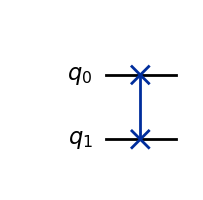
\includegraphics[width=0.3\textwidth]{../images/swap-gate.png}
    \caption{SWAP Gate}
    \label{fig:swap}
\end{figure}

In the operator Notation it is:
\begin{align*}
    SWAP\ket{00}&=\ket{00} \\
    SWAP\ket{01}&=\ket{10} \\
    SWAP\ket{10}&=\ket{01} \\
    SWAP\ket{11}&=\ket{11}
\end{align*}

It is represented by the matrix in the computational basis ($\ket{00},\ket{01},\ket{10},\ket{11}$) as:
\[
    SWAP=\begin{bmatrix}
        1 & 0 & 0 & 0 \\
        0 & 0 & 1 & 0 \\
        0 & 1 & 0 & 0 \\
        0 & 0 & 0 & 1
    \end{bmatrix}
\]
In Outer product representation, it can be written as:
\[
    SWAP=\ket{00}\bra{00}+\ket{01}\bra{10}+\ket{10}\bra{01}+\ket{11}\bra{11}
\]

Action of SWAP on general two - qubit $\ket{\psi} = \alpha\ket{00}+\beta\ket{01}+\gamma\ket{10}+\delta\ket{11}$ is:
\[
    \begin{bmatrix} 
        1 & 0 & 0 & 0 \\
        0 & 0 & 1 & 0 \\
        0 & 1 & 0 & 0 \\
        0 & 0 & 0 & 1
    \end{bmatrix}\begin{bmatrix}
        \alpha \\
        \beta \\
        \gamma \\
        \delta
    \end{bmatrix}=\begin{bmatrix}
        \alpha \\
        \gamma \\
        \beta \\
        \delta
    \end{bmatrix}=\alpha\ket{00}+\gamma\ket{01}+\beta\ket{10}+\delta\ket{11}
\]

SWAP Gate can also be formed using CNOT gates as follows:
\begin{figure}[H]
    \centering
    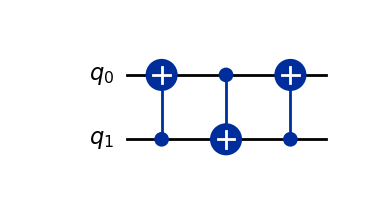
\includegraphics[width=0.3\textwidth]{../images/swap-gatemeth1.png}
    \caption{SWAP Gate using CNOT Gates}
    \label{fig:swap-cnot1}
\end{figure}
Or using CNOT gates as follows:
\begin{figure}[H]
    \centering
    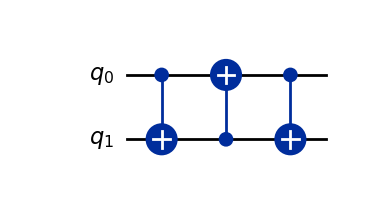
\includegraphics[width=0.3\textwidth]{../images/swap-gatemeth2.png}
    \caption{SWAP Gate using CNOT Gates}
    \label{fig:swap-cnot2}
\end{figure}

\subsection{Three-qubit Gates}
\subsubsection{CCNOT/Toffoli Gate}
It is a three qubit gate, also called as the CCNOT gate.
Here the 1st and 2nd Qubits are controlled and the 3rd Qubit is target.
The truth table is as in table \ref{tab:toffoli}.
\begin{table}[H]
    \centering
    \begin{tabular}{|c|c|c|}
        \hline
        Input & Output\\
        \hline
        $\ket{000}$ & $\ket{000}$\\
        $\ket{001}$   & $\ket{001}$\\
        $\ket{010}$   & $\ket{010}$\\
        $\ket{011}$  & $\ket{011}$\\
        $\ket{100}$ & $\ket{100}$\\
        $\ket{101}$   & $\ket{101}$\\
        $\ket{110}$   & $\ket{111}$\\
        $\ket{111}$  & $\ket{110}$\\
        \hline
    \end{tabular}
    \caption{Truth Table for Toffoli Gate}
    \label{tab:toffoli}
\end{table}
For the table in \ref{tab:toffoli}, the 1st and 2nd Qubits are control and the 3rd Qubit is target.
Thus, the Toffoli gate flips the target qubit if the control qubits are $\ket{1}$.
The code for the Toffoli Gate is as follows:
\begin{lstlisting}[language=Python]
from qiskit import QuantumRegister, ClassicalRegister, QuantumCircuit
from numpy import pi

qreg_q = QuantumRegister(3, 'q')
circuit = QuantumCircuit(qreg_q)

circuit.ccx(qreg_q[0], qreg_q[1], qreg_q[2])

circuit.draw(output='mpl')#.savefig('../images/ccx-gate.png')
\end{lstlisting}

The circuit symbol is as shown in figure \ref{fig:toffoli}.
\begin{figure}[H]
    \centering
    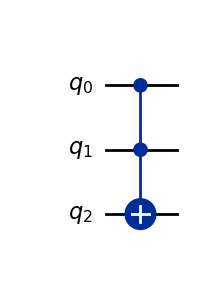
\includegraphics[width=0.3\textwidth]{../images/ccx-gate.png}
    \caption{Toffoli Gate}
    \label{fig:toffoli}
\end{figure}
In this figure \ref{fig:toffoli}, the first and second qubits are control and the third qubit is target.
If the first and second qubits are $\ket{1}$, then the third qubit is flipped. The Toffoli Gate
is a gate which flips the target qubit if the control qubits are $\ket{1}$.

In the operator Notation it is:
\begin{align*}
    CCX\ket{000}&=\ket{000} \\
    CCX\ket{001}&=\ket{001} \\
    CCX\ket{010}&=\ket{010} \\
    CCX\ket{011}&=\ket{011} \\
    CCX\ket{100}&=\ket{100} \\
    CCX\ket{101}&=\ket{101} \\
    CCX\ket{110}&=\ket{111} \\
    CCX\ket{111}&=\ket{110}
\end{align*}

It is represented by the matrix in the computational basis 
($\ket{000},\ket{001},\ldots,\ket{110},\ket{111}$) as:
\[
    CCX=\begin{bmatrix}
        1 & 0 & 0 & 0 & 0 & 0 & 0 & 0 \\
        0 & 1 & 0 & 0 & 0 & 0 & 0 & 0 \\
        0 & 0 & 1 & 0 & 0 & 0 & 0 & 0 \\
        0 & 0 & 0 & 1 & 0 & 0 & 0 & 0 \\
        0 & 0 & 0 & 0 & 1 & 0 & 0 & 0 \\
        0 & 0 & 0 & 0 & 0 & 1 & 0 & 0 \\
        0 & 0 & 0 & 0 & 0 & 0 & 0 & 1 \\
        0 & 0 & 0 & 0 & 0 & 0 & 1 & 0
    \end{bmatrix}
\]
In Outer product representation, it can be written as:
\begin{align*}
    CCX&=\ket{000}\bra{000}+\ket{001}\bra{001}+\ket{010}\bra{010}+\ket{011}\bra{011} \\
    &+\ket{100}\bra{100}+\ket{101}\bra{101}+\ket{110}\bra{111}+\ket{111}\bra{110}
\end{align*}

Action of CCX on general three - qubit $\ket{\psi} = \alpha\ket{000}+\beta\ket{001}+\gamma\ket{010}+\delta\ket{011}+\epsilon\ket{100}+\zeta\ket{101}+\eta\ket{110}+\theta\ket{111}$ is:
\[
    \begin{bmatrix} 
        1 & 0 & 0 & 0 & 0 & 0 & 0 & 0 \\
        0 & 1 & 0 & 0 & 0 & 0 & 0 & 0 \\
        0 & 0 & 1 & 0 & 0 & 0 & 0 & 0 \\
        0 & 0 & 0 & 1 & 0 & 0 & 0 & 0 \\
        0 & 0 & 0 & 0 & 1 & 0 & 0 & 0 \\
        0 & 0 & 0 & 0 & 0 & 1 & 0 & 0 \\
        0 & 0 & 0 & 0 & 0 & 0 & 0 & 1 \\
        0 & 0 & 0 & 0 & 0 & 0 & 1 & 0
    \end{bmatrix}\begin{bmatrix}
        \alpha \\
        \beta \\
        \gamma \\
        \delta \\
        \epsilon \\
        \zeta \\
        \eta \\
        \theta
    \end{bmatrix}=\begin{bmatrix}
        \alpha \\
        \beta \\
        \gamma \\
        \delta \\
        \epsilon \\
        \zeta \\
        \theta \\
        \eta
    \end{bmatrix}=\alpha\ket{000}+\beta\ket{001}+\ldots+\zeta\ket{101}+\theta\ket{110}+\eta\ket{111}
\]

\subsubsection{CSWAP/Fredkin Gate}\label{qgate:cswap}
It is a three qubit gate, also called as the CSWAP gate.
Here the 1st Qubit is control and the 2nd and 3rd Qubits are target.
The truth table is as in table \ref{tab:fredkin}.
\begin{table}[H]
    \centering
    \begin{tabular}{|c|c|c|}
        \hline
        Input & Output\\
        \hline
        $\ket{000}$ & $\ket{000}$\\
        $\ket{001}$   & $\ket{001}$\\
        $\ket{010}$   & $\ket{010}$\\
        $\ket{011}$  & $\ket{011}$\\
        $\ket{100}$ & $\ket{100}$\\
        $\ket{101}$   & $\ket{110}$\\
        $\ket{110}$   & $\ket{101}$\\
        $\ket{111}$  & $\ket{111}$\\
        \hline
    \end{tabular}
    \caption{Truth Table for Fredkin Gate}
    \label{tab:fredkin}
\end{table}
For the table in \ref{tab:fredkin}, the 1st Qubit is control and the 2nd and 3rd Qubits are target.
Thus, the Fredkin gate swaps the states of the 2nd and 3rd qubits if the control qubit is $\ket{1}$.
The code for the Fredkin Gate is as follows:
\begin{lstlisting}[language=Python]
from qiskit import QuantumRegister, ClassicalRegister, QuantumCircuit
from numpy import pi

qreg_q = QuantumRegister(3, 'q')
circuit = QuantumCircuit(qreg_q)

circuit.cswap(qreg_q[0], qreg_q[2], qreg_q[1])

circuit.draw(output='mpl')#.savefig('../images/cswap-gate.png')
\end{lstlisting}

The circuit symbol is as shown in figure \ref{fig:fredkin}.
\begin{figure}[H]
    \centering
    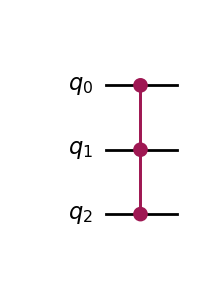
\includegraphics[width=0.3\textwidth]{../images/cswap-gate.png}
    \caption{Fredkin Gate}
    \label{fig:fredkin}
\end{figure}
In this figure \ref{fig:fredkin}, the first qubit is control and the second and third qubits are target.
If the first qubit is $\ket{1}$, then the second and third qubits are swapped. The Fredkin Gate
is a gate which swaps the states of the 2nd and 3rd qubits if the control qubit is $\ket{1}$.

In the operator Notation it is:
\begin{align*}
    CSWAP\ket{000}&=\ket{000} \\
    CSWAP\ket{001}&=\ket{001} \\
    CSWAP\ket{010}&=\ket{010} \\
    CSWAP\ket{011}&=\ket{011} \\
    CSWAP\ket{100}&=\ket{100} \\
    CSWAP\ket{101}&=\ket{110} \\
    CSWAP\ket{110}&=\ket{101} \\
    CSWAP\ket{111}&=\ket{111}
\end{align*}

It is represented by the matrix in the computational basis ($\ket{000},\ket{001},\ldots,\ket{110},\ket{111}$) as:
\[
    CSWAP=\begin{bmatrix}
        1 & 0 & 0 & 0 & 0 & 0 & 0 & 0 \\
        0 & 1 & 0 & 0 & 0 & 0 & 0 & 0 \\
        0 & 0 & 1 & 0 & 0 & 0 & 0 & 0 \\
        0 & 0 & 0 & 1 & 0 & 0 & 0 & 0 \\
        0 & 0 & 0 & 0 & 1 & 0 & 0 & 0 \\
        0 & 0 & 0 & 0 & 0 & 0 & 1 & 0 \\
        0 & 0 & 0 & 0 & 0 & 1 & 0 & 0 \\
        0 & 0 & 0 & 0 & 0 & 0 & 0 & 1
    \end{bmatrix}
\]
In Outer product representation, it can be written as:
\begin{align*}
    CSWAP&=\ket{000}\bra{000}+\ket{001}\bra{001}+\ket{010}\bra{010}+\ket{011}\bra{011} \\
    &+\ket{100}\bra{100}+\ket{101}\bra{110}+\ket{110}\bra{101}+\ket{111}\bra{111}
\end{align*}

Action of CSWAP on general three - qubit $\ket{\psi} = \alpha\ket{000}+\beta\ket{001}+\gamma\ket{010}+\delta\ket{011}+\epsilon\ket{100}+\zeta\ket{101}+\eta\ket{110}+\theta\ket{111}$ is:
\[
    \begin{bmatrix} 
        1 & 0 & 0 & 0 & 0 & 0 & 0 & 0 \\
        0 & 1 & 0 & 0 & 0 & 0 & 0 & 0 \\
        0 & 0 & 1 & 0 & 0 & 0 & 0 & 0 \\
        0 & 0 & 0 & 1 & 0 & 0 & 0 & 0 \\
        0 & 0 & 0 & 0 & 1 & 0 & 0 & 0 \\
        0 & 0 & 0 & 0 & 0 & 0 & 1 & 0 \\
        0 & 0 & 0 & 0 & 0 & 1 & 0 & 0 \\
        0 & 0 & 0 & 0 & 0 & 0 & 0 & 1
    \end{bmatrix}\begin{bmatrix}
        \alpha \\
        \beta \\
        \gamma \\
        \delta \\
        \epsilon \\
        \zeta \\
        \eta \\
        \theta
    \end{bmatrix}=\begin{bmatrix}
        \alpha \\
        \beta \\
        \gamma \\
        \delta \\
        \epsilon \\
        \zeta \\
        \theta \\
        \eta
    \end{bmatrix}=\alpha\ket{000}+\beta\ket{001}+\ldots+\zeta\ket{101}+\theta\ket{110}+\eta\ket{111}
\]

We can construct Fredkin gate using CNOT and Toffoli gate as shown in the figure \ref{fig:fredkin-cnot1}.
\begin{figure}[H]
    \centering
    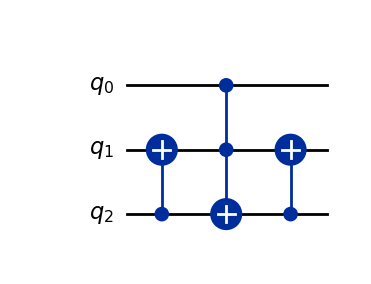
\includegraphics[width=0.3\textwidth]{../images/cswap-gatemeth1.png}
    \caption{Fredkin Gate using CNOT and Toffoli Gates}
    \label{fig:fredkin-cnot1}
\end{figure}

\begin{importantnote}
    Applying a gate on a superposition state is the same as applying the gate on each of the basis states and then superposing the results.
    This is because, the gate is a linear operator and the superposition is a linear combination of the basis states. 
    Thus, the gate can be applied on each of the basis states and then the results can be superposed. For example, Consider a superposition state $\ket{\psi}=\alpha\ket{0}+\beta\ket{1}$.
    If we apply a gate $U$ on this state, then the output will be $U\ket{\psi}=U(\alpha\ket{0}+\beta\ket{1})=\alpha U\ket{0}+\beta U\ket{1}$.
    Thus, the gate can be applied on each of the basis states and then the results can be superposed. This, can also be thought that since U is a $2 \times 2$ matrix and $\ket{0}$ and $\ket{1}$ are $2 \times 1$ column vectors, 
    multiplying $U(\alpha\ket{0}+\ket{1})$ is same as $\alpha U\ket{0}+\beta U\ket{1}$ Since Matrix multiplication is distributive. 

    For example, say CNOT gate needs to be applied on a superposition of two bits $\ket{\psi}=\alpha\ket{00}+\beta\ket{01}+\gamma\ket{10}+\delta\ket{11}$.
    Then the output will be $CNOT\ket{\psi}=CNOT(\frac{\ket{00}+\ket{11}}{\sqrt{2}})=\frac{CNOT\ket{00}+CNOT\ket{11}}{\sqrt{2}}$.
    which will thus be $\frac{\ket{00}+\ket{10}}{\sqrt{2}}$.
    In the matrix form, 
    \[
        CNOT\ket{\psi}=CNOT\left(\frac{\ket{00}+\ket{11}}{\sqrt{2}}\right)=\begin{bmatrix}
            1 & 0 & 0 & 0 \\
            0 & 1 & 0 & 0 \\
            0 & 0 & 0 & 1 \\
            0 & 0 & 1 & 0
        \end{bmatrix}\frac{1}{\sqrt{2}}\left(\begin{bmatrix}
            1 \\
            0 \\
            0 \\
            0
        \end{bmatrix}+\begin{bmatrix}
            0 \\
            0 \\
            0 \\
            1
        \end{bmatrix}\right)
    \]
    \[=\frac{1}{\sqrt{2}}\left(\begin{bmatrix}
        1 & 0 & 0 & 0 \\
        0 & 1 & 0 & 0 \\
        0 & 0 & 0 & 1 \\
        0 & 0 & 1 & 0
    \end{bmatrix}\begin{bmatrix}
        1 \\
        0 \\
        0 \\
        0
    \end{bmatrix}+\begin{bmatrix}
        1 & 0 & 0 & 0 \\
        0 & 1 & 0 & 0 \\
        0 & 0 & 0 & 1 \\
        0 & 0 & 1 & 0
    \end{bmatrix}\begin{bmatrix}
        0 \\
        0 \\
        0 \\
        1
    \end{bmatrix}\right)
    \]
    \[
    =(CNOT\frac{1}{\sqrt{2}}\ket{00}+CNOT\frac{1}{\sqrt{2}}\ket{11})=\frac{1}{\sqrt{2}}CNOT\ket{00}+\frac{1}{\sqrt{2}}CNOT\ket{11}
    \]
    \[
        =\frac{1}{\sqrt{2}}\left(\begin{bmatrix}
            1 \\
            0 \\
            0 \\
            0
        \end{bmatrix}+\begin{bmatrix}
            0 \\
            0 \\
            1 \\
            0
        \end{bmatrix}\right)=\frac{1}{\sqrt{2}}\begin{bmatrix} 1 \\ 0 \\ 1 \\ 0 \end{bmatrix} =\frac{1}{\sqrt{2}}\left(\ket{00}+\ket{10}\right)
    \]
    Thus, applying a gate on a superposition is the same as applying the gate on the basis states of the superposition. Thus, the gate can be applied on each of the basis states and then the results can be superposed
    in the same linear combination as that in which the state $\ket{\psi}$ was superposed.
\end{importantnote}
\section{Quantum Circuits}
\begin{example}
    Consider the quantum circuit as shown in figure \ref{fig:qcircuit1}.
    \begin{figure}[H]
        \centering
        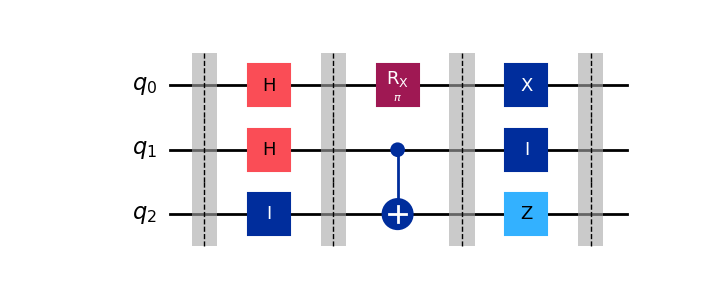
\includegraphics[width=0.8\textwidth]{../images/qcircuit1.png}
        \caption{Quantum Circuit}
        \label{fig:qcircuit1}
    \end{figure}
    \begin{enumerate}
        \item Make Reverse circuit of the given circuit.
        \item Write the output of the circuit for the input $\ket{010}$.
        \item Write complete circuit as Unitary Matrix.
        \item Write reverse circuit as Unitary Matrix.
        \item Compute output using Unitary matrix of circuit.
    \end{enumerate}
    \begin{enumerate}
        \item Note that excpet for the rotation gate all the other gates are their own inverses. Thus, the reverse circuit is as shown in figure \ref{fig:qcircuit1-rev}.
        \begin{figure}[H]
            \centering
            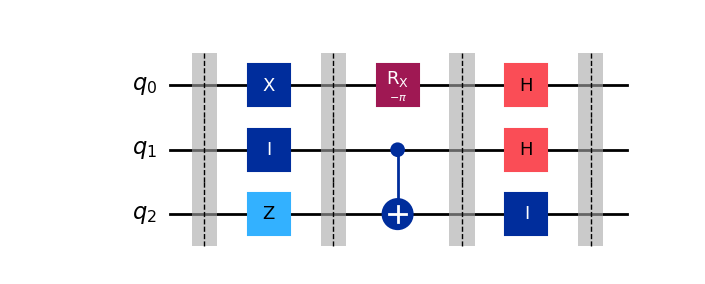
\includegraphics[width=0.8\textwidth]{../images/qcircuit1-rev.png}
            \caption{Reverse Quantum Circuit}
            \label{fig:qcircuit1-rev}
        \end{figure}
        If we place the two circuits side by side, we will get the input back. Thus it will act like an Identity matrix.
        \item As shown in the figure \ref{fig:qcircuit1} the circuit has been divded into parts for easy computation. At the first barrier, the input is $\ket{010}$.
        After applying the gates, at the second stage the output will be:
        \begin{align*}
            (H \otimes H \otimes I)(\ket{010})&=H\ket{0} \otimes H\ket{1}\otimes I\ket{0}\\
            &=\frac{1}{\sqrt{2}}(\ket{0}+\ket{1})\otimes\frac{1}{\sqrt{2}}(\ket{0}-\ket{1})\otimes\ket{0}\\
            &=\frac{1}{2}(\ket{000}-\ket{010}+\ket{100}-\ket{110})
        \end{align*}
        After this, the third stage requires the application of the RX gate on the first qubit and CNOT gate with 2nd qubit as control and 3rd qubit as target.
        The output after this stage will be:
        \begin{align*}
            (RX \otimes CX)(\frac{1}{2}(\ket{000}-\ket{010}+\ket{100}-\ket{110}))&=\frac{1}{2}(RX\ket{0} \otimes CX\ket{00}-RX\ket{0} \otimes CX\ket{10}\\
            &+RX\ket{1}\otimes CX\ket{00}-RX\ket{1}\otimes CX\ket{10})\\
            &=\frac{\ket{100}-\ket{111}-\ket{000}+\ket{011}}{2}
        \end{align*}
        Here the action of RXx is $RX\ket{0}=\ket{1}$, $RX\ket{1}=-\ket{0}$.
        Now we apply the last stage which involves applying X gate on the first qubit and Z gate on the 3rd qubits.
        \begin{align*} 
            (X \otimes I \otimes Z)\frac{\ket{100}-\ket{111}-\ket{000}+\ket{011}}{2}&=\frac{1}{2}(X\ket{1} \otimes I\ket{0} \otimes Z\ket{0}-X\ket{1}\otimes \\
            & I\ket{1}\otimes Z\ket{1}-X\ket{0}\otimes I\ket{0}\otimes Z\ket{0}+X\ket{0}\otimes I\ket{1}\\
            &\otimes Z\ket{1})\\
            &=\frac{1}{2}(\ket{000}+\ket{011}-\ket{100}-\ket{111})
        \end{align*}
        Thus, the state of the qubits after passing through the circuit.
        In the matrix form, it can be written as:
        \[
            \frac{1}{2}\begin{bmatrix} 1 \\ 0 \\ 0 \\ 1 \\ -1 \\ 0 \\ 0 \\-1 \end{bmatrix}
        \]
        \item In order to find the Unitary matrix for the complexte circuit, we are required to find the unitary matrices corresponding to 
        the individual stages and multiply them to get the final Unitary Matrix.
        For the first stage, we have two Hadamard gates acting on first and second qubit and an Identity gate. Thus, we are required to find,
        \begin{align*}
            S_1 &= H \otimes H \otimes I\\
            &= \frac{1}{\sqrt{2}}\begin{bmatrix} 1 & 1 \\ 1 & -1 \end{bmatrix} \otimes \frac{1}{\sqrt{2}}\begin{bmatrix} 1 & 1 \\ 1 & -1 \end{bmatrix} \otimes \begin{bmatrix} 1 & 0 \\ 0 & 1 \end{bmatrix}\\
        \end{align*}
        Thus, doing this the overall matrix will be:
        \[
            S_1 = \frac{1}{2}\begin{bmatrix}
                1 & 0 & 1 & 0 & 1 & 0 & 1 & 0 \\
                0 & 1 & 0 & 1 & 0 & 1 & 0 & 1 \\
                1 & 0 & -1 & 0 & 1 & 0 & -1 & 0 \\
                0 & 1 & 0 & -1 & 0 & 1 & 0 & -1 \\
                1 & 0 & 1 & 0 & -1 & 0 & -1 & 0 \\
                0 & 1 & 0 & 1 & 0 & -1 & 0 & -1 \\
                1 & 0 & -1 & 0 & -1 & 0 & 1 & 0 \\
                0 & 1 & 0 & -1 & 0 & -1 & 0 & 1 \\
            \end{bmatrix}
        \]
        For stage 2, we are required to find,
        \begin{align*}
            S_2 &= RX \otimes CX\\
            &= \begin{bmatrix} 0 & -1 \\ 1 & 0 \end{bmatrix} \otimes \begin{bmatrix} 1 & 0 & 0 & 0 \\
            0 & 1 & 0 & 0 \\
            0 & 0 & 0 & 1 \\
            0 & 0 & 1 & 0 \end{bmatrix} \\
        \end{align*}
        In the matrix form, we get:
        \[
            S_2=\begin{bmatrix}
                0 & 0 & 0 & 0 & -1 & 0 & 0 & 0 \\
                0 & 0 & 0 & 0 & 0 & -1 & 0 & 0 \\
                0 & 0 & 0 & 0 & 0 & 0 & 0 & -1 \\
                0 & 0 & 0 & 0 & 0 & 0 & -1 & 0 \\
                1 & 0 & 0 & 0 & 0 & 0 & 0 & 0 \\
                0 & 1 & 0 & 0 & 0 & 0 & 0 & 0 \\
                0 & 0 & 0 & 1 & 0 & 0 & 0 & 0 \\
                0 & 0 & 1 & 0 & 0 & 0 & 0 & 0 \\
            \end{bmatrix}
        \]
        For stage 3, we are required to find,
        \begin{align*}
            S_3 &= X \otimes I \otimes Z \\
            &= \begin{bmatrix} 0 & 1 \\ 1 & 0 \end{bmatrix} \otimes \begin{bmatrix} 1 & 0 \\ 0 & 1 \end{bmatrix} \otimes \begin{bmatrix} 1 & 0 \\ 0 & -1 \end{bmatrix} \\
            &= \begin{bmatrix} 0 & 0 & 0 & 0 & 1 & 0 & 0 & 0 \\
                0 & 0 & 0 & 0 & 0 & -1 & 0 & 0 \\
                0 & 0 & 0 & 0 & 0 & 0 & 1 & 0 \\
                0 & 0 & 0 & 0 & 0 & 0 & 0 & -1 \\
                1 & 0 & 0 & 0 & 0 & 0 & 0 & 0 \\
                0 & -1 & 0 & 0 & 0 & 0 & 0 & 0 \\
                0 & 0 & 1 & 0 & 0 & 0 & 0 & 0 \\
                0 & 0 & 0 & -1 & 0 & 0 & 0 & 0 \\
            \end{bmatrix} 
        \end{align*}
        Finally, we are required to calculate the product of the three matrices to get the overall matrix.
        \begin{align*} 
            U &= S_3S_2S_1 \\
            &= \frac{1}{2}\begin{bmatrix} 
                1 & 0 & 1 & 0 & 1 & 0 & 1 & 0 \\
                0 & -1 & 0 & -1 & 0 & -1 & 0 & -1 \\
                0 & 1 & 0 & -1 & 0 & 1 & 0 & -1 \\
                -1 & 0 & 1 & 0 & -1 & 0 & 1 & 0 \\
                -1 & 0 & -1 & 0 & 1 & 0 & 1 & 0 \\
                0 & 1 & 0 & 1 & 0 & -1 & 0 & -1 \\
                0 & -1 & 0 & 1 & 0 & 1 & 0 & -1 \\
                1 & 0 & -1 & 0 & -1 & 0 & 1 & 0 \\
            \end{bmatrix}
        \end{align*}
        \item The Unitary matrix for the reverse circuit will be the Transpose conjugate of the given circuit i.e. the transpose conjugate of the matrix found in the previous part.
        \[
            U^{\dagger}=\frac{1}{2}\begin{bmatrix} 
                1 & 0 & 0 & -1 & -1 & 0 & 0 & 1 \\
                0 & -1 & 1 & 0 & 0 & 1 & -1 & 0 \\
                1 & 0 & 0 & 1 & -1 & 0 & 0 & -1 \\
                0 & -1 & -1 & 0 & 0 & 1 & 1 & 0 \\
                1 & 0 & 0 & -1 & 1 & 0 & 0 & -1 \\
                0 & -1 & 1 & 0 & 0 & -1 & 1 & 0 \\
                1 & 0 & 0 & 1 & 1 & 0 & 0 & 1 \\
                0 & -1 & -1 & 0 & 0 & -1 & -1 & 0 \\
            \end{bmatrix}
        \]
        Thus, the matrix for the reverse circuit.
        \item The output of the circuit can be found by multiplying the input with the Unitary matrix of the circuit.
        \[
            U\begin{bmatrix} 0 \\ 0 \\ 1 \\ 0 \\ 0 \\ 0 \\ 0 \\ 0 \end{bmatrix}=\frac{1}{2}\begin{bmatrix} 1 \\ 0 \\ 0 \\ 1 \\ -1 \\ 0 \\ 0 \\ -1 \end{bmatrix}
        \]
        which can be verified as the same output from the previous part.
    \end{enumerate}
\end{example}

\chapter{Entanglement}
Given a state of multiple entangled qubit, one cannot express individual qubit seperately.
For example, consid the state $\ket{\psi} = \frac{\ket{00}+\ket{11}}{\sqrt{2}}$, cannot be expressed as some $\ket{\phi} \otimes \ket{\chi}$,
$\ket{\phi}=\alpha \ket{0} + \beta \ket{1}$ and $\ket{\chi}=\gamma \ket{0} + \delta \ket{1}$ i.e. no value of $\alpha, \beta, \gamma, \delta$ exists.The
n the states are called entangled.

On the contrary some states can be seperated into individual qubit states, such states are called separable states.
For example, consider the state $\ket{\psi} = \frac{\ket{00}+\ket{01}}{\sqrt{2}}$, can be expressed as $\ket{0} \otimes \frac{\ket{0}+\ket{1}}{\sqrt{2}}$, here
$\alpha =1 ,\beta =0,\gamma = \frac{1}{\sqrt{2}},\delta = \frac{1}{\sqrt{2}}$.

Given an Entangled state of multiple qubit, measuring any qubit individuall reveals all other qubits. 
For example, conisder $\ket{\psi}=\frac{\ket{00}+\ket{11}}{\sqrt{2}}$, thus suppose we measure only one qubit, i.e.
say we measure the first qubit. Then the probability of the first qubit being $\ket{0}$ is $|\frac{1}{\sqrt{2}}|^2=\frac{1}{2}$ and the probability of the first qubit being $\ket{1}$ is $|\frac{1}{\sqrt{2}}|^2=\frac{1}{2}$.
Now suppose we find that the first qubit is $\ket{0}$, then the state of the quantum system after measurement will be $\ket{00}$, thus the state of the second qubit will be $\ket{0}$.
Similarly, if we find that the first qubit is $\ket{1}$, then the state of the quantum system after measurement will be $\ket{11}$, thus the state of the second qubit will be $\ket{1}$.
This, we can see that measuring one qubit reveals the state of the other qubit. This is called entanglement.

But, in case of seperable qubits measuring one qubit will not reveal the state of the second qubit. For example, consider the state $\ket{\psi}=\frac{\ket{00}+\ket{01}}{\sqrt{2}}$,
if we measure the first qubit, then the probability of the first qubit being $\ket{0}$ is $|\frac{1}{\sqrt{2}}|^2+|\frac{1}{\sqrt{2}}|^2=1$ and the probability of the first qubit being $\ket{1}$ is $0$.
Thus, if we find that the first qubit is $\ket{0}$, then the state of the quantum system after measurement will be $\frac{\ket{00}+\ket{01}}{\sqrt{2}}$, thus the state of the second qubit will be $\ket{0}$ with probability $\frac{1}{2}$ and 
will be in state $\ket{1}$ with probability $\frac{1}{2}$. Thus, the state of the second qubit cannot be revealed. The measurement on the first qubit does not reveal any information of the state of the second qubit. 

\section{Bell States/EPR Pairs}
We have four Bell states, which are also called as EPR states. These are:
\begin{align*}
    \ket{\Phi^+}&=\ket{\beta_{00}}=\frac{\ket{00}+\ket{11}}{\sqrt{2}} \\
    \ket{\Phi^-}&=\ket{\beta_{10}}=\frac{\ket{00}-\ket{11}}{\sqrt{2}} \\
    \ket{\Psi^+}&=\ket{\beta_{01}}=\frac{\ket{01}+\ket{10}}{\sqrt{2}} \\
    \ket{\Psi^-}&=\ket{\beta_{11}}=\frac{\ket{01}-\ket{10}}{\sqrt{2}} \\
\end{align*}
The general formula for Bell states is:
\[
    \ket{\beta_{xy}}=\frac{\ket{0y}+(-1)^x\ket{1\bar{y}}}{\sqrt{2}}
\]
where $\bar{y}$ is the negation of $y$. Thus, we can find any Bell state using the above formula for 
any given input $x \in \{0,1\}$ and $y\ in \{0,1\}$.
We can create these bell states using quantum circuits as shown in figure \ref{fig:bell-states}.
\begin{figure}[H]
    \centering
    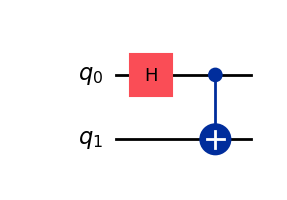
\includegraphics[width=0.8\textwidth]{../images/bell-states.png}
    \caption{Bell States}
    \label{fig:bell-states}
\end{figure}
For example, suppose we wish to apply the circuit on state $\ket{01}$. Then the state after applying the
operation $H \otimes I$ will be $\frac{\ket{0}+\ket{1}}{\sqrt{2}}\otimes\ket{1}=\frac{\ket{01}+\ket{11}}{\sqrt{2}}$.
Similarly, the state after applying the operation $CX$ will be $\frac{\ket{01}+\ket{10}}{\sqrt{2}}=\beta_{01}$.

\begin{example}
    Given the state $\ket{\psi}=\frac{\ket{01}-\ket{10}}{\sqrt{2}}$, find whether the state is entangled or not.
    We proove this by contradiction, Assume that $\ket{\psi}$ can be written seperately as $\alpha\ket{0}+\beta\ket{1} \otimes \gamma\ket{0}+\delta\ket{1}$.
    Thus, we get, 
    \begin{align*}
        \frac{\ket{01}-\ket{10}}{\sqrt{2}}&=\alpha\ket{0}+\beta\ket{1} \otimes \gamma\ket{0}+\delta\ket{1}\\
        &=\alpha\gamma\ket{00}+\alpha\delta\ket{01}+\beta\gamma\ket{10}+\beta\delta\ket{11}\\
    \end{align*}
    Comparing the equations we have, 
    \begin{align*}
        \alpha\gamma&=0 \\
        \alpha\delta&=\frac{1}{\sqrt{2}} \\
        \beta\gamma&=-\frac{1}{\sqrt{2}} \\
        \beta\delta&=0 \\
    \end{align*}
    No solution exists for the above equations, thus the given state is entangled as it cannot be written as a tensor product of two states.
\end{example}
Entanglement has applications in Teleportation and Superdense Coding which will be discussed next.
To get back the original input state from the Bell states we can use the following Circuit.
\begin{figure}[H]
    \centering
    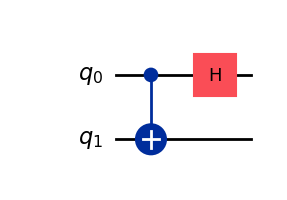
\includegraphics[width=0.8\textwidth]{../images/bell-states-rev.png}
    \caption{Reverse Bell States}
    \label{fig:bell-states-rev}
\end{figure}
Here, we have used a reverse CNOT gate i.e. inverse of CNOT gate which is the CNOT gate since it's a self-inverse gate (Hermitian and Unitary).
Then we use the reverse Hadamard gate which is Hadamard Gate on the first qubit and the circuit will give back the original input state. (Hadmard gate is also self-inverse).

\section{No Cloning Theorem}
One of the counter-intuitive consequences of the laws of Quantum Mechanics is that 
it is impossible to create an exact copy of an arbitrary unknown quantum state. This is called the No Cloning Theorem.
More formally, 
\begin{theorem}
    Given an arbitrary unknown quantum state $\ket{\psi}$, it is impossible to create an exact copy of the state $\ket{\psi}$
    i.e. create the state $\ket{\psi}\ket{\psi}$. More precisely, it is impossible to start with two qubits in the state $\ket{\phi} \otimes \ket{0}$ and transform them to the state $\ket{\phi} \otimes \ket{\phi}$.
\end{theorem}
\begin{proof}
    From the Postulate 2: Evolution Postulate given in section \ref{subsection:Postulate 2}, from Axiom of Quantum Mechanics, for this to be possible there must be a Unitary transformation U such that $U\ket{\phi}\otimes \ket{0} = \ket{\phi}\otimes \ket{\phi}$. Thus, in order to prove that it is impossible to do so, it suffices to prove that no such unitary transformation exists. We start with proving that no such unitary transformation exists that can achieve this simultaneously for two states $\ket{\phi}=\alpha_0\ket{0}+\alpha_1\ket{1}$ and $\ket{\psi}=\beta_0\ket{0}+\beta_1\ket{1}$.

    Recall that a unitary transformation is a rotation of the Hilbert Space, and therefore necessarily preserves inner products. To be more precise, consider two quantum states: 
    \[
    \ket{\phi} \otimes \ket{0}= \alpha_0\ket{00}+\alpha_1\ket{10}
    \]
    and 
    \[\ket{\psi}\otimes \ket{0}=\beta_0\ket{00}+\beta_1\ket{10}
    \]
    Then, the inner product between them is given by 
    \[
    \braket{\phi0|\psi0}=\alpha^*_0\beta_0+\alpha^*_1\beta_1=\braket{\phi|\psi}
    \]
    Now consider the quantum states, 
    \begin{align*}
    \ket{\phi} \otimes \ket{\phi}&=(\alpha_0\ket{0}+\alpha_1\ket{1})\otimes (\alpha_0\ket{0}+\alpha_1\ket{1})\\
    &=\alpha^2_0\ket{00}+\alpha_0\alpha_1\ket{01}+\alpha_1\alpha_0\ket{10}+\alpha^2_1\ket{11}
    \end{align*}
    and
    \begin{align*}
    \ket{\psi}\otimes \ket{\psi}&=(\beta_0\ket{0}+\beta_1\ket{1})\otimes (\beta_0\ket{0}+\beta_1\ket{1})\\
    &=\beta^2_0\ket{00}+\beta_0\beta_1\ket{01}+\beta_1\beta_0\ket{10}+\beta^2_1\ket{11}
    \end{align*}
    Their inner product is 
    \begin{align*}
    \braket{\phi\phi|\psi\psi}&=(\bra{00}\alpha^{*2}_0+\bra{01}\alpha^*_0\alpha^*_1+\bra{10}\alpha^*_1\alpha^*_0+\bra{11}\alpha^{*2}_1)(\beta^2_0\ket{00}+\beta_0\beta_1\ket{01}+\beta_1\beta_0\ket{10}+\beta^2_1\ket{11})\\
    &=\alpha^{*2}_0\beta^2_0+\alpha^*_0\alpha^*_1\beta_0\beta_1+\alpha^*_1\alpha_0\beta_1\beta_0+\beta^2_0\beta^2_1\\
    &=(\alpha^*_0\beta_0+\alpha^*_1\beta_1)^2
    \end{align*}

    Now let us assume that we have a Unitary operator U and the two arbitrary quantum states $\ket{\phi}$ and $\ket{\psi}$ such that the action of U is defined as follows:
    \[
    \ket{\phi}\otimes \ket{0} \xrightarrow{U} \ket{\phi}\otimes \ket{\phi}
    \]
    \[
    \ket{\psi}\otimes \ket{0} \xrightarrow{U}\ket{\psi}\otimes \ket{\psi}
    \]
    Thus, clearly operator U corresponds to an operator which performs copying arbitrary quantum states.
    Since we are performing the same unitary transformation on both the states $\ket{\phi}$ and $\ket{\psi}$, thus the inner product before and after transformation must be the same, as a Unitary transformation corresponds to rotations in the complex Hilbert space. Their inner product before transformation is 
    \[
    \braket{\phi0|\psi0}=\alpha^*_0\beta_0+\alpha^*_1\beta_1
    \]
    Their inner product after the transformation will be:
    \[
    \braket{\phi\phi|\psi\psi}=(\alpha^*_0\beta_0+\alpha^*_1\beta_1)^2=\braket{\phi0|\psi0}^2=\braket{\phi|\psi}^2
    \]
    Thus, before transformation we had the inner product as $\braket{\phi|psi}$ and after the transformation we have the inner product as $\braket{\phi|\psi}^2$. Thus, in general, $\braket{\phi|\psi}\neq \braket{\phi|\psi}^2$ (It is equal only in the case when $\braket{\phi|\psi}=0$ or $1$ i.e. both the quantum states are orthonormal). Since, this is not true for any two arbitrary quantum states, thus our assumption that such a Unitary transformation U exists is wrong. Thus, by contradiction, we have proved that such a Unitary transformation U does not exists, hence, it is impossible to copy an arbitrary unknown quantum state $\ket{\phi}$ or in other words, to be more precise, no such unitary transformation $U$ exists which can perform the following transformation of $\ket{\phi} \otimes \ket{0} \rightarrow \ket{\phi} \otimes \ket{\phi}$.
\end{proof}

\section{Applications of Entanglement}
\subsection{Quantum Teleportation}
Alice and Bob are two friends. 
They get together and create a Bell state $\beta_{00}$ and then 
distribute the quantum system. One qubit stays with Alice (say $\ket{\beta_A}$) 
and the other qubit goes to Bob (say $\ket{\beta_B}$).
Now Bob moves 100,000 light years away. Now, say Alive wishes to send Bob an Arbitrary state $\ket{\psi}$ to Bob.\\
\\
The teleportation protocol is as follows:
\begin{enumerate}
    \item Alice and Bob create a Bell state $\beta_{00}$. It is as shown in the figure \ref{fig:teleportation1} which has both the inputs $q_0=\ket{0}$ and $q_1=\ket{0}$.
    \begin{figure}[H]
        \centering
        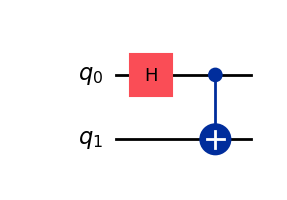
\includegraphics[width=0.5\textwidth]{../images/teleportation1.png}
        \caption{Creating Bell States}
        \label{fig:teleportation1}
    \end{figure}
    The state of the circuit after applying this state is the Bell state which is given as $\beta_{00}=\frac{\ket{00}+\ket{11}}{\sqrt{2}}$.
    Now, say the outcome of the first bit be $\ket{\beta_A}$ which is the state of the first qubit goes to Alice and the outcome of the second bit be $\ket{\beta_B}$ which is the state of the second qubit which goes to Bob.
    \item Alice applies a CNOT gate with the input state $\ket{\psi}$ as the control qubit and the state $\ket{\beta_A}$ as the target qubit. Then Alice applies a Hadamard gate on the input state $\ket{\psi}$. This is as shown in the figure \ref{fig:teleportation2} with $q_0=\ket{\psi}$ and $q_1=\ket{\beta_A}$.
    \begin{figure}[H]
        \centering
        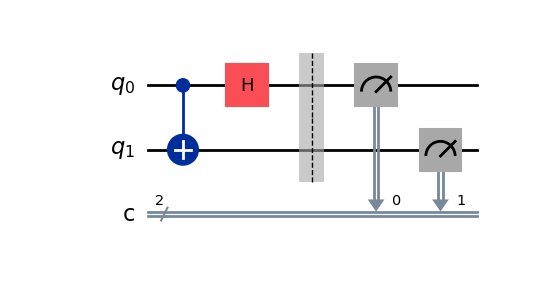
\includegraphics[width=0.5\textwidth]{../images/teleportation2.png}
        \caption{Alice's Operations}
        \label{fig:teleportation2}
    \end{figure}
    Thus the state here, is $\ket{\psi}\ket{\beta_{00}}$. Let the state $\ket{\psi}=\alpha\ket{0}+\beta\ket{1}$.
    Thus, 
    \[
        \ket{\psi}\ket{\beta_{00}}=(\alpha\ket{0}+\beta\ket{1})\otimes \frac{\ket{00}+\ket{11}}{\sqrt{2}}=\frac{\alpha\ket{000}+\alpha\ket{011}+\beta\ket{100}+\beta\ket{111}}{\sqrt{2}}
    \]
    Now applying CNOT with first bit as control bit and the second bit as the targt bit we get,
    \[
        \frac{\alpha\ket{000}+\alpha\ket{011}+\beta\ket{110}+\beta\ket{101}}{\sqrt{2}}
    \]
    Now, applying Hadamard gate on the first bit we get,
    \[
        \frac{\alpha\ket{000}+\alpha\ket{100}+\alpha\ket{011}+\alpha\ket{111}+\beta\ket{010}-\beta\ket{110}+\beta\ket{001}-\beta\ket{101}}{2}
    \]
    We further simplify this by considering only the first two qubits, we get,
    \[
        \frac{1}{2}\left[\ket{00}(\alpha\ket{0}+\beta\ket{1})+\ket{01}(\alpha\ket{1}+\beta\ket{0})+\ket{10}(\alpha\ket{0}-\beta\ket{1})+\ket{11}(\alpha\ket{1}-\beta\ket{0})\right]
    \]
    Now Alice does measurement of the first two qubits. Remember that the qubit $\ket{\psi}$ is already normalized i.e. $|\alpha|^2+|\beta|^2=1$. The probability of the first two qubits being $\ket{00}$ is $|\frac{\alpha}{2}|^2+|\frac{\beta}{2}|^2=\frac{|\alpha|^2+|\beta|^2}{4}=\frac{1}{4}$, similarly, 
    the probability of the first two qubits being $\ket{10}$ is $\frac{1}{4}$, the probability of the first two qubits being $\ket{01}$ is $\frac{1}{4}$ and the probability of the first two qubits being $\ket{11}$ is $\frac{1}{4}$.
    
    Suppose upon measuring the two qubits by Alice they collapsed to $\ket{00}$, then the state of the system will be:
    \[
        \alpha\ket{000}+\beta\ket{001}=\ket{00}\otimes (\alpha\ket{0}+\beta{\ket{1}})
    \]
    Suppose upon measuring the two qubits by Alice they collapsed to $\ket{10}$, then the state of the system will be:
    \[
        \alpha\ket{100}-\beta\ket{101}=\ket{10}\otimes (\alpha\ket{0}-\beta\ket{1})
    \]
    Suppose upon measuring the two qubits by Alice they collapsed to $\ket{01}$, then the state of the system will be:
    \[
        \alpha\ket{011}+\beta\ket{010}=\ket{01}\otimes (\alpha\ket{1}+\beta\ket{0})
    \]
    Suppose upon measuring the two qubits by Alice they collapsed to $\ket{11}$, then the state of the system will be:
    \[
        \alpha\ket{111}-\beta\ket{110}=\ket{11}\otimes (\alpha\ket{1}-\beta\ket{0})
    \]
    All of the above are possible with a probability of $\frac{1}{4}$.
    \item Now Alice sends the result of the measurement to Bob. Bob applies the necessary operations to get the original state $\ket{\psi}=\alpha\ket{0}+\beta\ket{1}$.
    
    \begin{itemize}
        \item Suppose Alice measured the first two qubits to be $\ket{00}$, then Bob applies no operation.
        \[
            \alpha\ket{000}+\beta\ket{001}=\ket{00}\otimes (\alpha\ket{0}+\beta\ket{1})
        \]
        \item Suppose Alice measured the first two qubits to be $\ket{10}$, then Bob applies the Z gate on his qubit to get the original state.
        \[ 
            Z(\alpha\ket{100}-\beta\ket{101})=\alpha\ket{100}+\beta\ket{101}=\ket{10}\otimes (\alpha\ket{0}+\beta\ket{1})
        \]
        \item Suppose Alice measured the first two qubits to be $\ket{01}$, then Bob applies the X gate on his qubit to get the original state.
        \[ 
            X(\alpha\ket{011}+\beta\ket{010})=\alpha\ket{010}+\beta\ket{011}=\ket{01}\otimes (\alpha\ket{0}+\beta\ket{1})
        \]
        \item Suppose Alice measured the first two qubits to be $\ket{11}$, then Bob applies the X and Z gate on his qubit to get the original state.
        \[ 
            Z(X(\alpha\ket{111}-\beta\ket{110}))=\alpha\ket{110}+\beta\ket{111}=\ket{11}\otimes (\alpha\ket{0}+\beta\ket{1})
        \]
    \end{itemize}
    Thus, we have teleported the unkown state $\ket{\psi}$ from Alice to Bob. Note that during this protocol, the Bell state of the qubits is destroyed upon measurement by Alice and thus, cannot be done again.
\end{enumerate}
The final Teleportation circuit is as shown in the figure \ref{fig:teleportation}.
\begin{figure}[H]
    \centering
    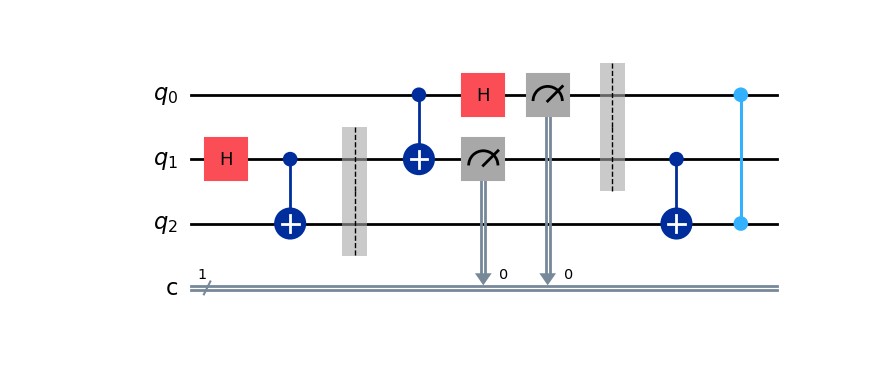
\includegraphics[width=0.8\textwidth]{../images/teleportation.png}
    \caption{Teleportation Circuit}
    \label{fig:teleportation}
\end{figure}
We can see from the figure that the measurement ouput from the Alice's qubits act as control bits for appling Z and X gate.
If the first qubit is 1 then we apply the Z gate, if the second qubit is 1 then we apply the X gate. Based on the Alice's output we can decide whether to apply  Thus the circuit shown in the figure \ref{fig:teleportation}, show that
after Alice's measurement the bits act as control bits for the operations to be applied by Bob.

\subsection{Superdence Coding}
In Superdense coding we can send from one place to another two classical bits but using only one qubit. 
Alice and Bob create a bell state $\beta_{00}$ and then distribute the qubits. Alice takes the first qubit and Bob takes the second qubit.
Bob now moves light years away. Alice now wishes to send two classical bits to Bob. The protocol is as follows:
\begin{enumerate}
    \item \textbf{Preparing Bell States: }Alice and Bob create a Bell state $\beta_{00}$.
    The state of the circuit after applying this state is the Bell state which is given as $\beta_{00}=\frac{\ket{00}+\ket{11}}{\sqrt{2}}$.
    Now, say the first bit be $\ket{\beta_A}$ which is the qubit that goes to Alice and the second bit be $\ket{\beta_B}$ which is the qubit which goes to Bob.
    \begin{figure}[H]
        \centering
        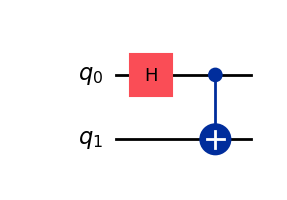
\includegraphics[width=0.5\textwidth]{../images/superdense-coding1.png}
        \caption{Creating Bell States}
        \label{fig:superdense1}
    \end{figure}
    This is how the Bell state is created shown in the figure \ref{fig:superdense1}.
    \item \textbf{Alice Encoding: } Alice applies the necessary operations to send the two classical bits to Bob.
    These operations are done on the first qubit which is with Alice as follows in the figure \ref{fig:superdense2}.
    \begin{figure}[H]
        \centering
        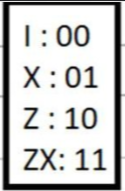
\includegraphics[width=0.3\textwidth]{../images/superdense-coding2.png}
        \caption{Alice's Encoding}
        \label{fig:superdense2}
    \end{figure}
    \begin{itemize}
        \item If Alice wishes to send $00$, then she applies no operation.
        \[
            \frac{\ket{00}+\ket{11}}{\sqrt{2}}
        \]
        \item If Alice wishes to send $01$, then she applies the Pauli - X gate on her portion of Bell state.
        \[
            X\left(\frac{\ket{00}+\ket{11}}{\sqrt{2}}\right)=\frac{\ket{10}+\ket{01}}{\sqrt{2}}
        \]
        \item If Alice wishes to send $10$, then she applies the Pauli-Z gate on the qubit.
        \[
            Z\left(\frac{\ket{00}+\ket{11}}{\sqrt{2}}\right)=\frac{\ket{00}-\ket{11}}{\sqrt{2}}
        \]
        \item If Alice wishes to send $11$, then she applies the Pauli-X and Pauli-Z gate on the qubit.
        \[
            X\left(Z\left(\frac{\ket{00}+\ket{11}}{\sqrt{2}}\right)\right)=\frac{\ket{10}-\ket{01}}{\sqrt{2}}
        \]

    \end{itemize}
    \item \textbf{Bob Decoding: }NOw Alice sends her portion of Bell state qubit to Bob. Bob then applies the necessary operations to get the two classical bits.
    Bob performs the following operations on the qubit he received from Alice:
    He applies CNOT gate with the first qubit (Qubit sent by Alice) as the control qubit and the second qubit as the target qubit. Then he applies Hadamard gate on the first qubit (Qubit sent by Alice).
    Then she performs the measurement. The measurement will give the two classical bits that Alice wished to send.
    This is as shown in the figure \ref{fig:superdense3}.
    \begin{figure}[H]
        \centering
        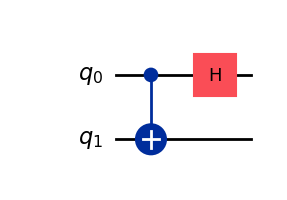
\includegraphics[width=0.5\textwidth]{../images/superdense-coding3.png}
        \caption{Bob's Decoding}
        \label{fig:superdense3}
    \end{figure}
    \begin{itemize}
        \item If Alice wished to send $00$, then the state of the system is currently $\frac{\ket{00}+\ket{11}}{\sqrt{2}}$. Thus, after applying the CNOT gate,
        \[
            CNOT\left(\frac{\ket{00}+\ket{11}}{\sqrt{2}}\right)=\frac{\ket{00}+\ket{10}}{\sqrt{2}}
        \]
        Now, after applying the Hadamard Gate on the first qubit we get,
        \[
            H\left(\frac{\ket{00}+\ket{10}}{\sqrt{2}}\right)=\frac{\ket{00}+\ket{10}+\ket{00}-\ket{10}}{2}=\ket{00}
        \]
        Thus, on measurement, the two classical bits are $00$.
        \item If Alice wished to send $01$, then the state of the system is currently $\frac{\ket{10}+\ket{01}}{\sqrt{2}}$. Thus, after applying the CNOT gate,
        \[
            CNOT\left(\frac{\ket{10}+\ket{01}}{\sqrt{2}}\right)=\frac{\ket{11}+\ket{01}}{\sqrt{2}}
        \]
        Now, after applying the Hadamard Gate on the first qubit we get,
        \[
            H\left(\frac{\ket{11}+\ket{01}}{\sqrt{2}}\right)=\frac{\ket{01}-\ket{11}+\ket{01}+\ket{11}}{2}=\ket{01}
        \]
        \item If Alice wished to send $10$, then the state of the system is currently $\frac{\ket{00}-\ket{11}}{\sqrt{2}}$. Thus, after applying the CNOT gate,
        \[
            CNOT\left(\frac{\ket{00}-\ket{11}}{\sqrt{2}}\right)=\frac{\ket{00}-\ket{10}}{\sqrt{2}}
        \]
        Now, after applying the Hadamard Gate on the first qubit we get,
        \[
            H\left(\frac{\ket{00}-\ket{10}}{\sqrt{2}}\right)=\frac{\ket{00}+\ket{10}-\ket{00}+\ket{10}}{2}=\ket{10}
        \]
        \item If Alice wished to send $11$, then the state of the system is currently $\frac{\ket{10}-\ket{01}}{\sqrt{2}}$. Thus, after applying the CNOT gate,
        \[
            CNOT\left(\frac{\ket{10}-\ket{01}}{\sqrt{2}}\right)=\frac{\ket{11}-\ket{01}}{\sqrt{2}}
        \]
        Now, after applying the Hadamard Gate on the first qubit we get,
        \[
            H\left(\frac{\ket{11}-\ket{01}}{\sqrt{2}}\right)=\frac{\ket{01}-\ket{11}-\ket{01}-\ket{11}}{2}=-\ket{11}
        \]
        Thus, upon measurement the two classical bits are $11$.
    \end{itemize}
\end{enumerate}

The final Superdense coding circuit is as shown in the figure \ref{fig:superdense-coding}.
% Add four subfigures
\begin{figure}[H]
    \centering
    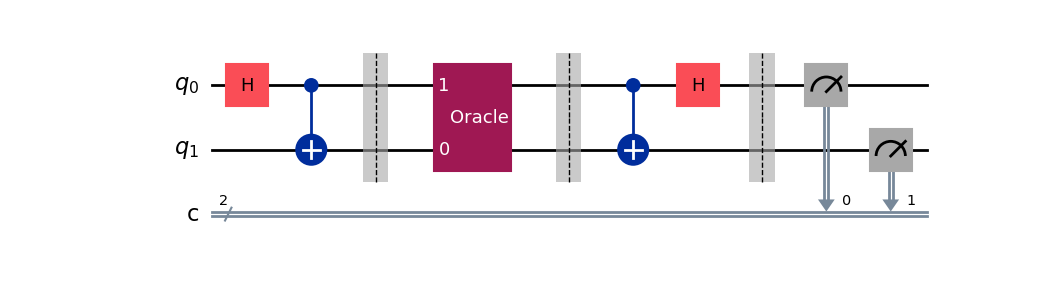
\includegraphics[width=0.8\textwidth]{../images/superdense-coding4.png}
    \caption{Superdense Coding Circuit}
    \label{fig:superdense-coding}
\end{figure}
 
\newpage

\chapter{Quantum Algorithms}
The following are the Quantum Algorithms are discussed in this section:
\begin{enumerate}
    \item Elitzur-Vaidman Bomb Detection Algorithm
    \item Deutsch's Algorithm
    \item Deutsch-Josza Algorithm
    \item Simon's Algorithm
    \item Shor's Algorithm
    \item Bernstein-Vazirani Algorithm
    \item Grover's Algorithm
    \item Quantum Fourier Transform
    \item Quantum Phase Estimation
\end{enumerate}
In order to understand Quantum Algorithms we must understand the Oracles and their working.
\section{Oracles}\label{sec:Oracles}
Consider a classical circuit representing a classical function $f$. 
Consider the classical function $f:\{0,1\}^n \rightarrow \{0,1\}^m$ which takes $n$ bits as input and gives $m$ bits as output.
\textbf{We can represent this classical function using a classical circuit}. (For the proof of this please refer to Applendix \ref{proof:classicalcomputations})
Thus, any classical boolean function $f:\{0,1\}^n \rightarrow \{0,1\}^m$ can be represented using a classical circuit as shown in the figure \ref{classicalcircuit}.
\begin{figure}[H]
    \centering
    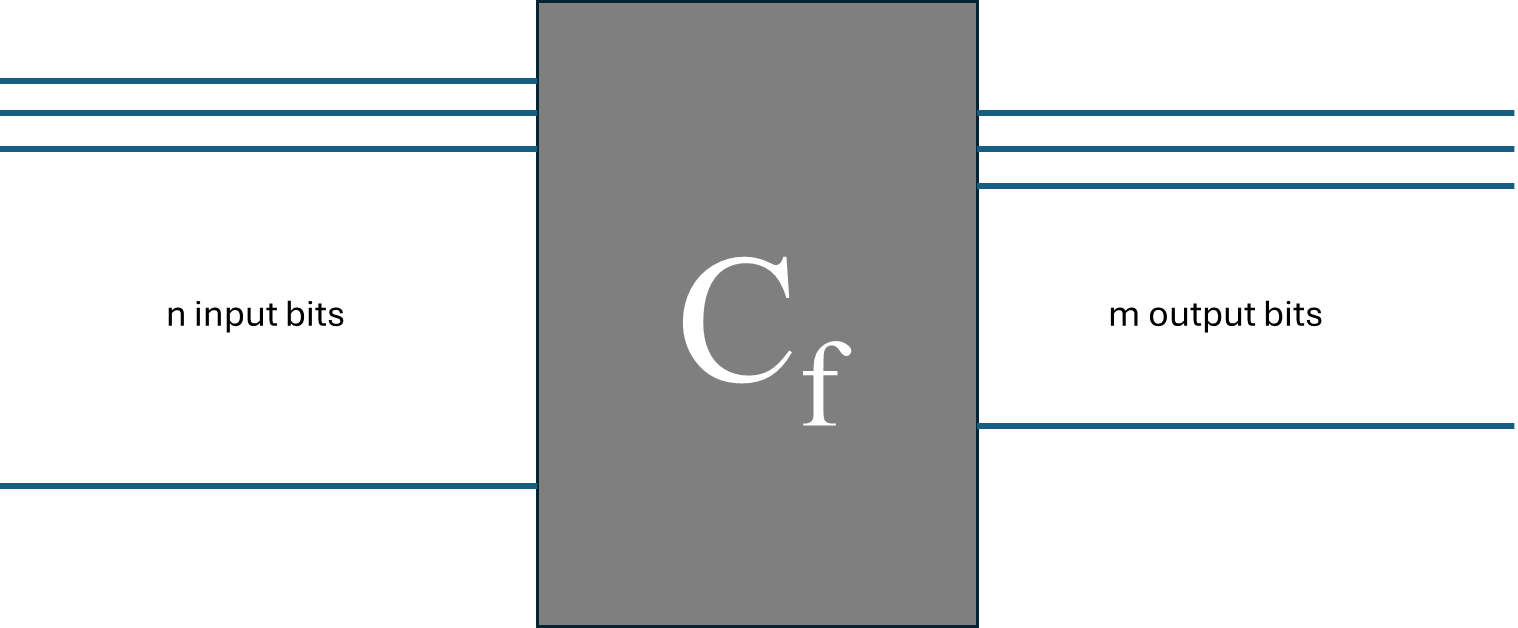
\includegraphics[width=0.8\textwidth]{../images/classicalcircuit.png}
    \caption{Classical Circuit}
    \label{classicalcircuit}
\end{figure}
But we are interested in Quantum Circuits. Thus, we are required to convert this classical circuit into a Quantum Circuit.
Recall, that a Quantum Circuit is a sequence of Quantum Gates. Since all the operations using quantum gates done on qubits  are untiary opertaions (thus, reversible),
and thus the Quantum circuit can be written as a product of Unitary quantum gates which is a Unitary matrix (product of unitary matrices is a unitary matrix). Thus, the Quantum Circuit is itself a Unitary Gate and hence reversible. Thus, the Quantum circuits are reversible.
Note that here the meaning of reversibility is that given the output of the circuit we can find the input of the circuit. This is because the Quantum Gates are Unitary and thus reversible.
Thus, a Gate is said to be reversible if given the output of the gate we can find the input of the gate. 

But, a classical circuit need not be necessarily reversible. Thus, we are required to convert the classical circuit into a reversible circuit in order to implement it on a Quantum Computer as a Quantum Circuit (Unitary Gates i.e. hence always reversible).
Thus, we are required to transform the classical circuit in order to make it reversible in order to implement it as a Unitary matrix made up of Quantum Gates (reversible since $U_f^{\dagger}=U_f^{-1}$).

This, can be done by transforming gates in a classical universal gate set to corresponding reversible quantum gates. Thus, then can we implement any classical circuit on a quantum computer. 
Note that a universal gate set is the set of gates which can be used to implement any classical circuit. There can be multiple gate set which form the universal gate sets. For example, the $\{NAND\}$ gate is a universal gate set,
$\{AND, NOT\}$ is another universal gate set. Thus, we can create any classical circuit using only the gates in the universal gate set. Now, if we are able to show that 
the gates in the universal gate set can be transformed into reversible quantum gates, then we can implement any classical circuit on a quantum computer using the corresponding reversible quantum gates. We can convert any classical circuit in terms of the universal gate sets and then 
replace the gates in the universal gate set with their corresponding reversible quantum gates to get the quantum circuit.

For the consideration let us take the Classical universal gate set $\{AND,NOT\}$. Here, NOT gate (refer Appendix \ref{cgate:NOT}) is already reversible 
becuase if we know the output of the NOT gate we can find the input. For example, if the output of the NOT gate is 1 then we know that the input was 0 and if the output of the NOT gate is 0 then we know that the input was 1. This is because NOT is a single input single output gate (number of inputs=number of outputs)
which negates the input. Thus, for the two inputs $0$ and $1$ we get the outputs $1$ and $0$ respectively. Thus, for finding the input from the given output we can simply negate that output to get the input (negation twice cancels out). Hence, the NOT gate is already a reversible gate. 
It's equivalent Quantum Gate is the Pauli-X gate which is also reversible. Thus, we can replace the NOT gate in the classical circuit with the Pauli-X gate in the Quantum Circuit.
Recall that the Pauli-X Gate is $\begin{bmatrix} 0 & 1 \\ 1 & 0 \end{bmatrix}$ and its action on $\ket{0}$ and $\ket{1}$ are $X\ket{0}=\ket{1}$ and $X\ket{1}=\ket{0}$
respectively. Thus, the Pauli-X gate is reversible and the quantum equivalent of the Classical NOT Gate.

Now, we are left with the AND gate. The AND gate is a two input single output gate i.e. It takes two inputs and gives one output. The output is 1 if and only if both the inputs are 1, else the output is 0 (refer Appendix \ref{cgate:AND}).
Thus, for the case when the output is 0 the input could be either $00$ or $01$ or $10$ but not $11$. For the output of 1 we definitely know that the input was $11$. 
But, for the output of $00$ we cannot determine the input. Thus, the AND gate is not reversible. Thus, we are required to convert the AND gate into a reversible gate in order to implement it on a Quantum Computer.
Thus, in order to create a reversible AND gate consider the control-Swap Gate (refer section \ref{qgate:cswap}). It takes three different inputs say
$\ket{x}$, $\ket{y}$ and $\ket{z}$. Say x acts as the control bit and y and z are the target bits. 
This, is as shown in the figure \ref{fig:cswap}
\begin{figure}[H]
    \centering
    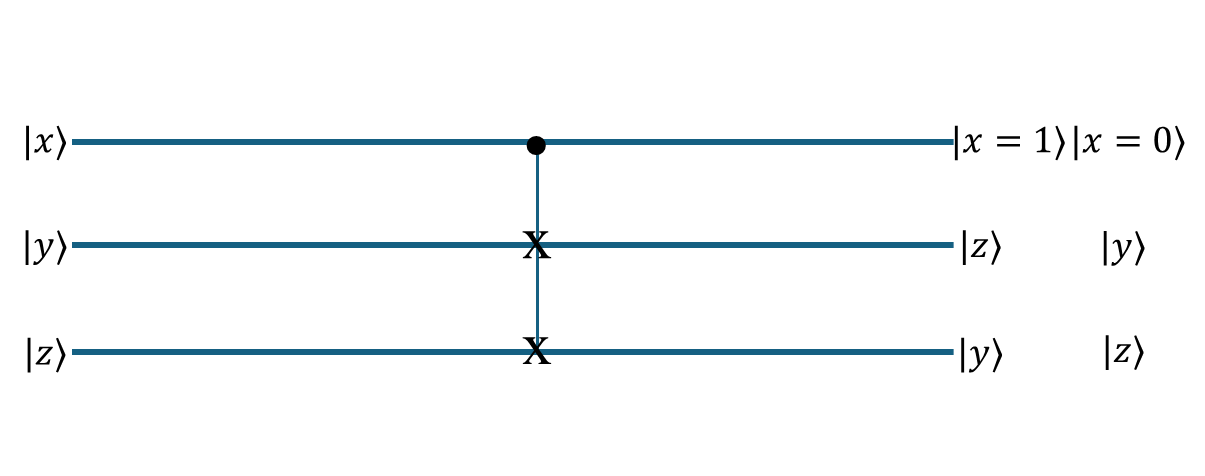
\includegraphics[width=0.8\textwidth]{../images/reversiblecswap.png}
    \caption{Control Swap Gate}
    \label{fig:cswap}
\end{figure}
Thus, if 
$x=1$ then the state of the system is swapped i.e. $\ket{y}$ and $\ket{z}$ are swapped, thus the output is $\ket{x},\ket{z},\ket{y}$. If $x=0$ then the state of the system remains the same $\ket{x},\ket{y},\ket{z}$.

Now in order to create reversible AND gate using the control-Swap gate we can do the following. Set the $\ket{z}=\ket{0}$.
Then, the output of the control-Swap gate will be $\ket{x},\ket{0},\ket{y}$ if $x=1$ and $\ket{x},\ket{y},\ket{0}$ if $x=0$.
This, output can also be written in a more compact form as $\ket{x},(\ket{0},\ket{y}),\ket{x \land y}$ where $\land$ is the AND operation. The second qubit can be either $\ket{0}$ or $\ket{y}$ depending on the value of $x$.
If $x=1$ then the second qubit will be $\ket{y}$ and if $x=0$ then the second qubit will be $\ket{0}$. This, output of the second qubit is refered to as junk which is a function of x i.e. $junk(x)$. This is as shown in the figure \ref{fig:reversibleand}.
\begin{figure}[H]
    \centering
    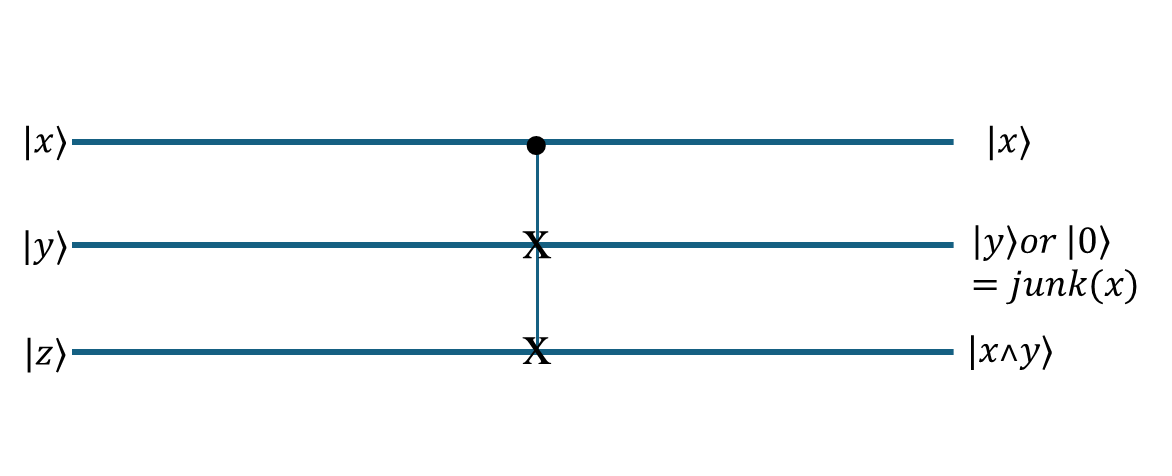
\includegraphics[width=0.8\textwidth]{../images/reversibleand.png}
    \caption{Reversible AND Gate}
    \label{fig:reversibleand}
\end{figure}
The truth table for the above circuit is as shown in the table \ref{tab:reversibleand}.
\begin{table}[H]
    \centering
    \begin{tabular}{|c|c|c|c|c|}
        \hline
        $x$ & $y$ & $0$ & $junk(x)$ & $x \land y$ \\
        \hline
        0 & 0 & 0 & 0 & 0 \\
        0 & 1 & 0 & 1 & 0 \\
        1 & 0 & 0 & 0 & 0 \\
        1 & 1 & 0 & 1 & 1 \\
        \hline
    \end{tabular}
    \caption{Reversible AND Gate}
    \label{tab:reversibleand}
\end{table}
Hence, we can clearly see that the output of the circuit is the same as the output of the AND gate. Thus, the above circuit is the reversible AND gate. 
Thus, using CSWAP gate as shown above we can convert the AND gate into a reversible gate. 

Thus, we can convert any classical circuit into a reversible circuit by replacing the gates in the universal gate set with their corresponding reversible quantum gates.
We replace NOT gate with the Pauli-X gate and the AND gate with the modified CSWAP Gate. 
Hence, any classical function can be implemented on a classical circuit (in terms of universal gate set $\{AND,NOT\}$) which then can be converted to a reversible circuit by replacing the gates in the universal gate set with their corresponding reversible quantum gates
($AND$ gate with Modified CSWAP and NOT gate with Pauli-X gate). Thus, for a general classical function with corresponding implementation in classical circuit as $C_f$ we would have a corresponding
quantum circuit $U_f$ which is the reversible version of the classical circuit $C_f$ thus, implementing the classical function $f$ on a quantum circuit by making it reversible. Here, we have converted the classical function $f$ to a reversible function $\tilde{f}$ which has number of inputs equal to the number of outputs, 
produces the same output as the classical function $f$ along with the input and some junk values as shown in the figure \ref{fig:classicaltoquantum}. \textbf{We can implement any classical function on a quantum circuit.}
\begin{figure}
    \centering
    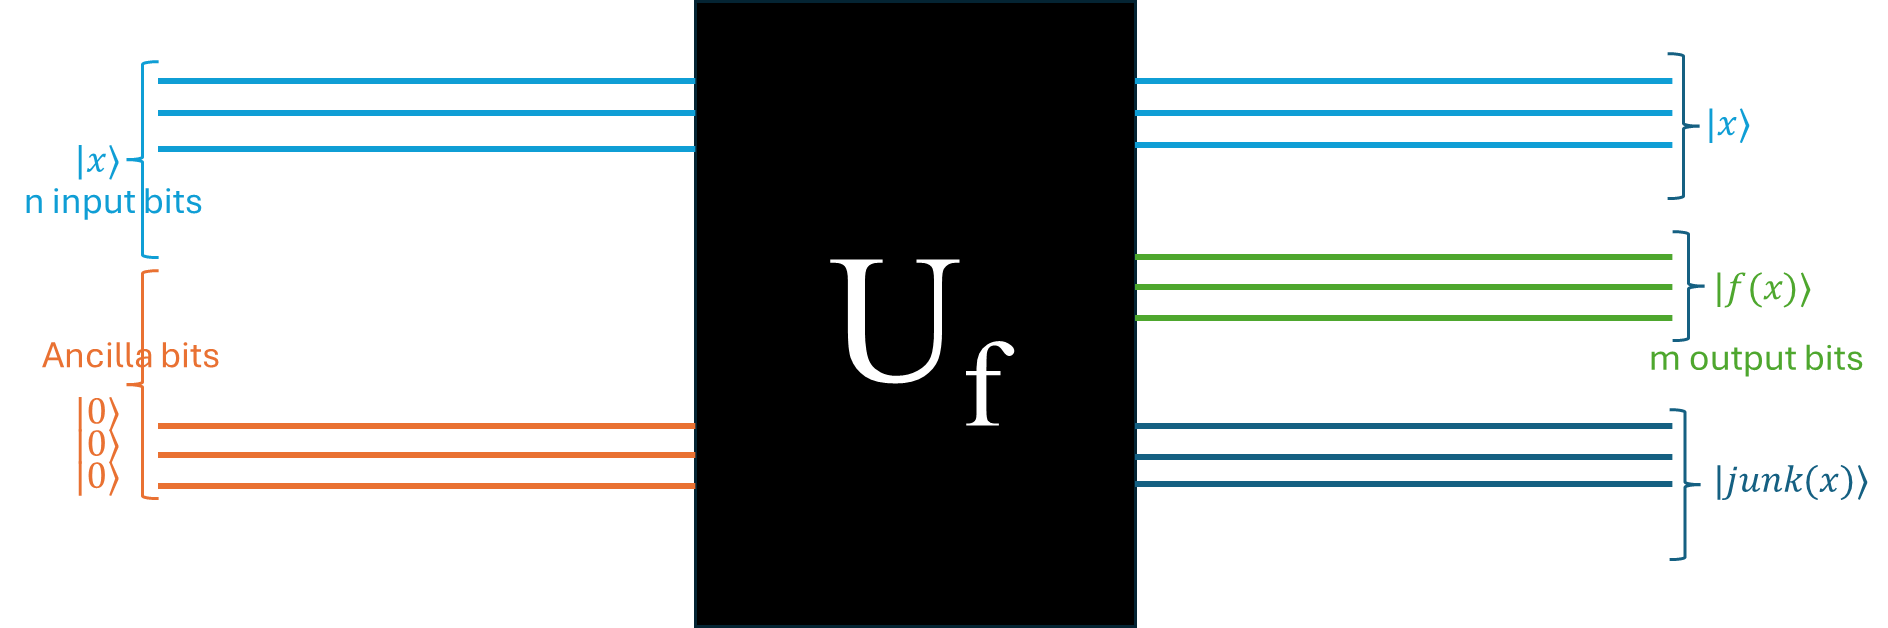
\includegraphics[width=0.8\textwidth]{../images/classicaltoquantum.png}
    \caption{Quantum Circuit}
    \label{fig:classicaltoquantum}
\end{figure}
The above figure shows the conversion of a classical circuit to a quantum circuit. 

Thus, a classical circuit when converted to a quantum circuit is as shown in the figure \ref{fig:classicaltoquantum}, it takes input $\ket{x}$ and along with it 
some ancilla bits (aka junk bits) and produces the output $\ket{x}$, $\ket{y \oplus f(x)}$ along with some junk bits $junk(x)$. We need to remove the junk since it consumes extra amount of qubits which is a waste of quantum resources and 
also the junk bits might get entangled with the output and any interference with environment may lead to decoherence or incorrect output and errors. Thus, we need to remove the junk bits.
This is done using the following circuit \ref{fig:quantumoracle}
\begin{figure}[H]
    \centering
    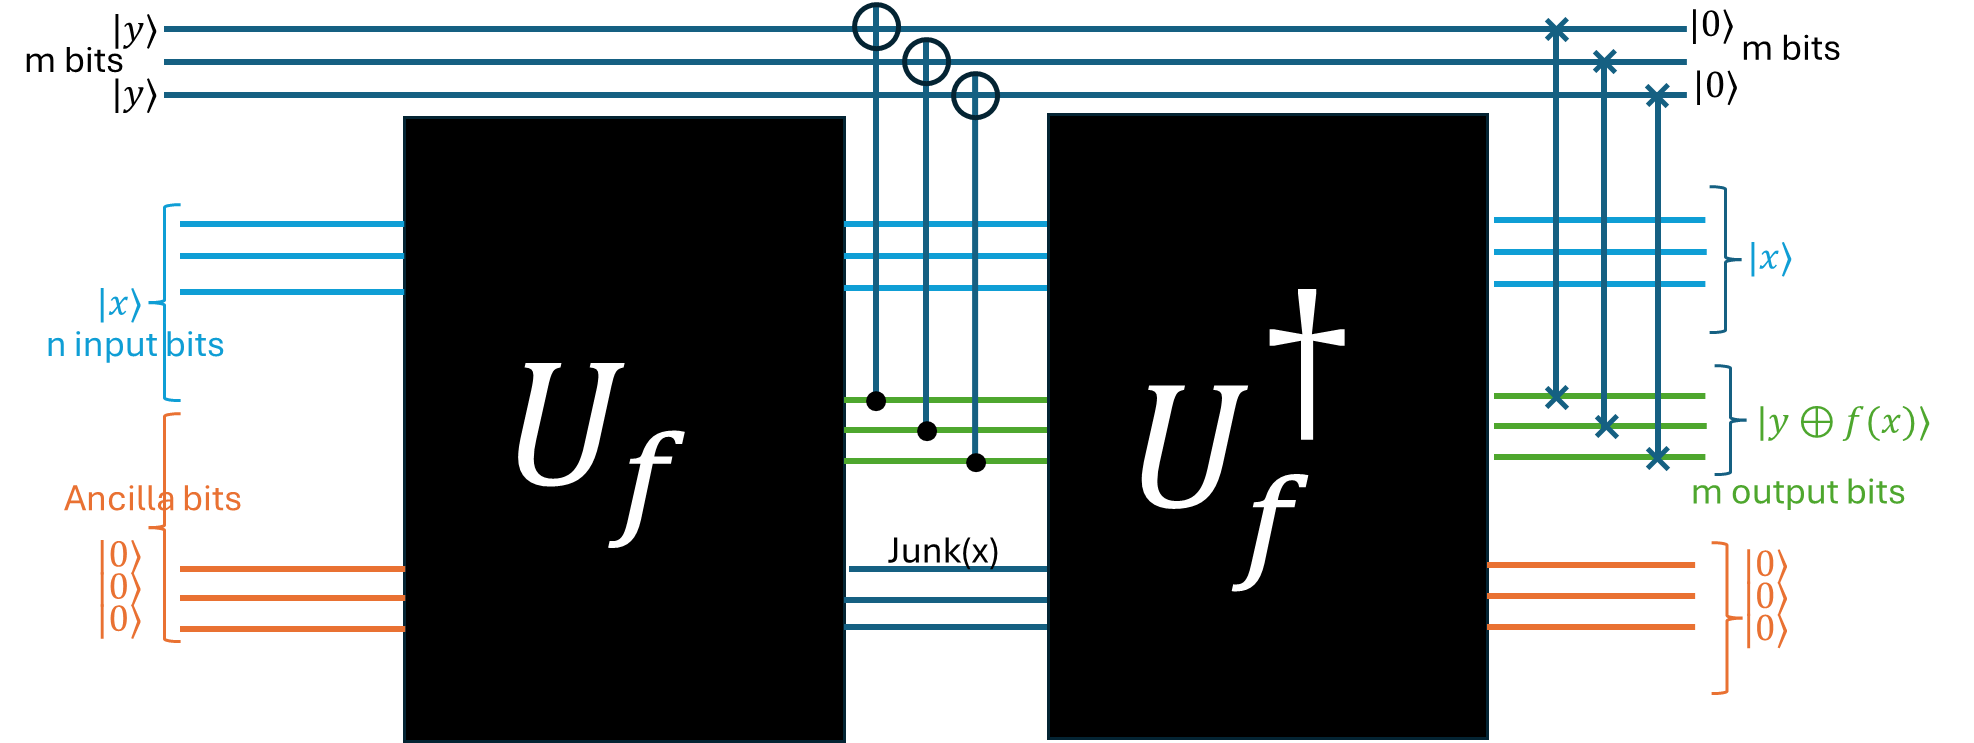
\includegraphics[width=0.8\textwidth]{../images/quantumoracle.png}
    \caption{Quantum Oracle}
    \label{fig:quantumoracle}
\end{figure}
Using this circuit it can be seen that the output of the entire circuit is $\ket{x},\ket{y\oplus f(x)}$ and the junk bits are are now $\ket{0}$ so that they can be used for other purposes in the circuit ahead. 
The output from the first Quantum Circuit $U_f$ is $\ket{x},\ket{y\oplus f(x)},junk(x)$. To remove the junk bits, it was done by first copying the output $\ket{f(x)}$ to the other (working bits) bits and then the output from the $U_f$ circuit was passed through its inverse $U_f^{-1}=U^{\dagger}_f$. Thus, upon passing through its inverse the output will be $\ket{x},\ket{0},\ket{0}$ since $U_f^{\dagger}$ is a reverse circuit and hence will make the outputs back to the inputs. 
Then the bits are swapped between as shown in the figure to get the desired output of 
$\ket{x},\ket{y\oplus f(x)},\ket{0},\ket{0}$ with no junk. Thus, the output of the circuit is the input $\ket{x}$ and the output $\ket{y\oplus f(x)}$. This entire thing is called an Oracle. 
Thus, we can imagine a Quantum Circuit which is an implementation of a classical fucntion $f$ as a black box which takes input $\ket{x}, \ket{y},\ket{0}$ and produces the output $\ket{x},\ket{y\oplus f(x)},\ket{0}$. 
For the sake of simpliicity we generally ignore the $\ket{0}$ in inputs and outputs. 

Thus, wheverer given a classical function $f$, we can make it as a reversible quantum function and thus, implmement
it as a quantum circuit using reversible quantum gates. This can be visualized as shown in the figure \ref{oracle}.
\begin{figure}[H]
    \centering
    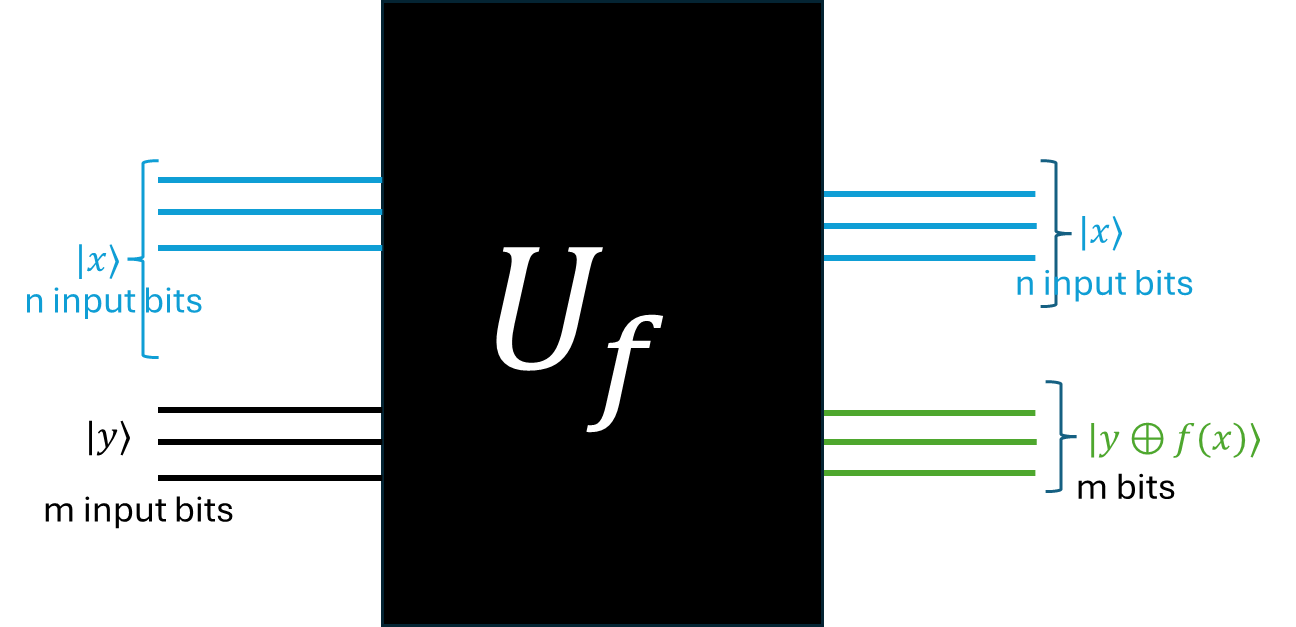
\includegraphics[width=0.8\textwidth]{../images/oracle.png}
    \caption{Oracle}
    \label{oracle}
\end{figure}

\section{Elitzur-Vaidman Bomb Detection Algorithm}
We are given a device which can be a working Bomb or dud. The devices takes a Quantum bit as input and produces an output.
If the device is a bomb, then the device performs a measurement on that qubit. If the outcome of the measurement is 1, then the bomb explodes, else the bomb does not explode.
If the device is dud, then the device does nothing i.e output is same as input.
We wish to determine whether the device is a bomb or dud without exploding the bomb. The Elitzur-Vaidman Bomb Detection Algorithm is as follows:
\begin{enumerate}
    \item \textbf{Approach 1: Naive Approach }\\We give the device naively the input of $\ket{0}$ and $\ket{1}$. 
    \begin{itemize} 
        \item \textbf{Case 1: Device is a Bomb}\\
        If we give device input of $\ket{0}$ then the output will also be $\ket{0}$ always, becuase the outcome of the measurement will be $\ket{0}$ so the bomb doesn't explode and returns $\ket{0}$. 
        If we give device inputof $\ket{1}$ then upon measurement the outcome will be $\ket{1}$ and the bomb explodes always.
        \item \textbf{Case 2: Device is a Dud}\\
        For the input of $\ket{0}$ if the device is a dud then the output is $\ket{0}$ since it does no operation on the input.
        For the input of $\ket{1}$ if the device is a dud then the output is $\ket{1}$ since it does no operation on the input.
    \end{itemize}
    To summarise the above approach, giving input $\ket{0}$ isof no help as it provides no information about the device since in both the cases if its a bomb or a dud the output will be $\ket{0}$. 
    Upon giving input $\ket{1}$ if the device is a dud then the output will be $\ket{1}$ and if the device is a bomb then the bomb will explode. Thus, it tells us whether the device is a bomb or a dud but if its a bomb it will explode. Thus, this approach is not useful since we can never deteact a working bomb.
    \item \textbf{Approach 2: Quantum Superposition Approach}\\
    Here we use a Hadamard Gate before and after the device. The circuit is as shown in the figure \ref{fig:elitzur-vaidman}.
    \begin{figure}[H]
        \centering
        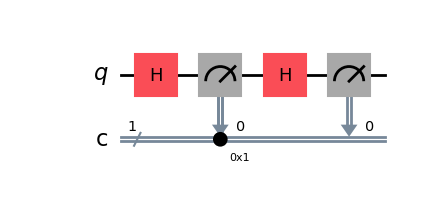
\includegraphics[width=0.5\textwidth]{../images/elitzur-vaidman.png}
        \caption{Elitzur-Vaidman Bomb Detection Algorithm}
        \label{fig:elitzur-vaidman}
    \end{figure}
    Here the first measurement is present if device is a bomb.
    \begin{itemize}
        \item \textbf{Case 1: Device is a Bomb}\\
        If we give input of $\ket{0}$ then upon passing thorugh the hadamard gate it will be $\ket{+}=\frac{\ket{0}+\ket{1}}{\sqrt{2}}$. As it passes through the device,
        it performs a measurement since its a bomb. Thus, the outcome of the measurement in computational basis will be $\ket{0}$ with probability $\frac{1}{2}$ and $\ket{1}$ with probability $\frac{1}{2}$.
        Thus, in the cases where the outcome is $\ket{0}$ the bomb will not explode and the output will then pass through another Hadamard gate which will give output as $\ket{+}$. Thus, upon final measurement we will get 
        $\ket{0}$ with probability $\frac{1}{2}$ and $\ket{1}$ with probability $\frac{1}{2}$. In the case where the measurement outcome is $\ket{1}$ the bomb will explode.

        \item \textbf{Case 2: Device is a Dud}\\
        If we give input of $\ket{0}$ then the upon passing through the hadamard gate it will be $\ket{+}=\frac{\ket{0}+\ket{1}}{\sqrt{2}}$. As it passes through the device, the device does nothing and the output will be $\ket{+}$.
        Then, we pass through the Hadamard gate which will output $\ket{0}$ and upon final measurement we will get the output as $\ket{0}$.
    \end{itemize}
    To summarize, the above approach, suppose there are a 1000 devices out of which probability of being a bomb is 50\%, thus, 500 are bombs and 500 are duds. If we given input $\ket{0}$ to all the devices. Then the output will be $\ket{0}$ for all the duds. 
    For the bombs, because of the measurement 50\% will detect $\ket{1}$ and will explode while the other $50\%$ will not explode and output $\ket{0}$. Thus, out of 500 bombs, 250 will explode and the rest 250 won't explode. 
    Then, the out of the bombs which didn't explode and which give outcomes as $\ket{0}$, it will pass thorugh a hadamard gate whose output will be $\ket{+}$ and thus upon final measurement we will get $\ket{0}$ with probability $\frac{1}{2}$ and $\ket{1}$ with probability $\frac{1}{2}$.
    Thus, out of the 250 bombs which didn't explode 50\% i.e. 125 of them will output$\ket{1}$ and the other 50\% i.e. 125 will output $\ket{0}$. 

    Thus, out of the 1000 devices we will get 250 bombs which will explode and out of the rest 750 devices we will get output of $\ket{0}$ for 625 (500 duds + 125 bombs which gave output $\ket{0}$) devices and output of $\ket{1}$ for 125 devices. Now, we are specifically interested in the cases where the output was $\ket{1}$ upon input $\ket{0}$. This is possible
    only in the case where the devices were bomb which didn't explode, since had it been a dud the output would have been $\ket{0}$. Thus the 125 cases where the ouptut was $\ket{1}$ upon input of $\ket{0}$ are the bombs which didn't explode. 
    Thus, out of the 500 bombs 250 of them exploded and we found 125 working bombs, and the other 125 bombs didn't explode but couldn't be identified among the duds. Thus, we found 25\% of the working bombs without exploding them. Or, we can say that the we can find a working bomb with a probability of $\frac{1}{8}$ out of all the given devices (or we can find a working bomb witout exploding given that the device is a bomb with probability $\frac{1}{4}$).
    
    \textbf{What if the input had been $\ket{1}$?: }The result will be the same as above. The only difference is that the output will be $\ket{1}$ for the duds and the bombs which didn't explode. Some of the bombs which didn't explode will output $\ket{0}$ and thus, can be detected as working bombs.
    
    \textbf{Thus, we can find a working bomb with a probability of $\frac{1}{8}$ (i.e. without exploding) out of all the given devices (or we can find a working bomb witout exploding given that the device is a bomb with probability $\frac{1}{4}$). But, recall that in this case $\frac{1}{2}$ (i.e. 250 bombs) of the bombs exploded and out of the other $\frac{1}{2}$ (i.e. 250 bombs) which didn't explode we only found $\frac{1}{2}$ (i.e. 125 bombs) of the working bombs, the rest $\frac{1}{2}$ (i.e. 125 bombs) didn't explode but couldn't be identified either.}

    \item \textbf{Elitzur-Vaidman Bomb Detection Algorithm: }\\
    Recall that we are measuring in orthnormal computational basis i.e. $\ket{0}$ and $\ket{1}$. Consider the Single-Qubit gate $R^Y_{\theta}$ which is defined as:
    \[
        R^Y_{\theta}=\begin{bmatrix}
            \cos\frac{\theta}{2} & -\sin\frac{\theta}{2} \\
            \sin\frac{\theta}{2} & \cos\frac{\theta}{2} \\
        \end{bmatrix}
    \]
    where $\theta$ is the angle of rotation. The $R^Y_{\theta}$ gate is a rotation gate about the Y-axis. The $R^Y_{\theta}$ gate is a unitary gate and thus preserves the norm of the vector as well as inner product. It is also a Hermitian gate. Thus, $R^Y_{\theta}$ is a self-inverse gate. $R^Y_{\theta}=(R^Y_{\theta})^{\dagger}=(R^Y_{\theta})^{-1}$.
    Thus, the action of $R^Y_{\theta}$ gate on the state $\ket{0}$ is as follows:
    \[
        R^Y_{\theta}\ket{0}=\begin{bmatrix}
            \cos\frac{\theta}{2} & -\sin\frac{\theta}{2} \\
            \sin\frac{\theta}{2} & \cos\frac{\theta}{2} \\
        \end{bmatrix}\begin{bmatrix}
            1 \\
            0 \\
        \end{bmatrix}=\begin{bmatrix}
            \cos\frac{\theta}{2} \\
            \sin\frac{\theta}{2} \\
        \end{bmatrix}=\cos\frac{\theta}{2}\ket{0}+\sin\frac{\theta}{2}\ket{1}
    \]
    Thus, upon measurement the probability of getting $\ket{0}$ is $|\cos\frac{\theta}{2}|^2$ and the probability of getting $\ket{1}$ is $|\sin\frac{\theta}{2}|^2$. Thus, the $R^Y_{\theta}$ gate is a rotation gate about the Y-axis by an angle $\theta$.
    Now clearly, for very small $\theta$, the probability of getting $\ket{0}$ is approximately $\cos \frac{\theta}{2}$.
    The circuit for Elitzur-Vaidman Bomb Detection Algorithm is as shown in the figure \ref{elitzur}.
    \begin{figure}[H]
        \centering
        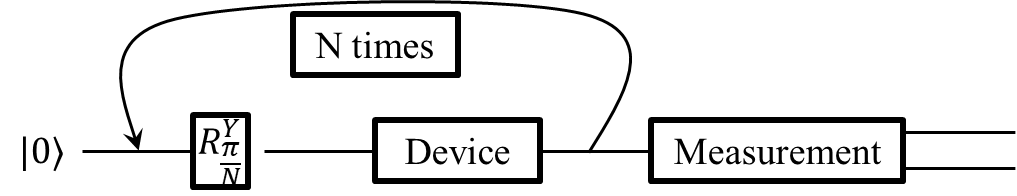
\includegraphics[width=0.8\textwidth]{../images/elitzur-vaidmanfinal.png}
        \caption{Elitzur-Vaidman Bomb Detection Algorithm}
        \label{elitzur}
    \end{figure}
    Thus, we we pass $\ket{0}$ through the $R^Y_{\theta}$ gate, the output will be $\cos\frac{\theta}{2}\ket{0}+\sin\frac{\theta}{2}\ket{1}$. 
    \begin{itemize}
        \item \textbf{Case 1:Device is a Dud}\\
        Now since the device is Dud, it will do nothing and after the first iteration, the output will be $\cos\frac{\pi}{2N}\ket{0}+\sin\frac{\pi}{2N}\ket{1}$.
        Now, for the second iteration it will be passed through the $R^Y_{\theta}$ gate again and the output will be:
        \[\begin{bmatrix}
            \cos\frac{\pi}{2N} & -\sin\frac{\pi}{2N} \\
            \sin\frac{\pi}{2N} & \cos\frac{\pi}{2N} \\
        \end{bmatrix}\begin{bmatrix}
            \cos\frac{\pi}{2N} \\
            \sin\frac{\pi}{2N} \\
        \end{bmatrix}=\begin{bmatrix}
            \cos^2\frac{\pi}{2N}-\sin^2\frac{\pi}{2N} \\
            2\cos\frac{\pi}{2N}\sin\frac{\pi}{2N} \\
        \end{bmatrix}=\cos\frac{\pi}{N}\ket{0}+\sin\frac{\pi}{N}\ket{1}\]
        Thus, after the second iteration the output will be $\cos\frac{\pi}{N}\ket{0}+\sin\frac{\pi}{N}\ket{1}$.
        Thus, after the kth iteration the output will be $\cos \frac{k\pi}{2N}\ket{0}+\sin \frac{k\pi}{2N}\ket{1}$.
        Thus, at the last Nth iteration it will be $\cos \frac{\pi}{2}\ket{0}+\sin \frac{\pi}{2}\ket{1}=\ket{1}$. Thus, upon the final measurement 
        the output will be $\ket{1}$. Thus, for the case when the device is a dud we will get $\ket{1}$ as the output.

        \item \textbf{Case 2: Device is a Bomb}\\
        Now since the device is a bomb, it will perform a measurement. Thus, after passing the input $\ket{0}$ through the rotation gate, the output will be $\cos\frac{\pi}{2N}\ket{0}+\sin\frac{\pi}{2N}\ket{1}$.
        Now since the device is a bomb, it performs a measurement and the measurement will be $\ket{0}$ with probability $\cos^2\frac{\pi}{2N}$ and $\ket{1}$ with probability $\sin^2\frac{\pi}{2N}$. Now consider for very large N,
        the probability of getting $\ket{0}$ is $\lim_{N\rightarrow \infty} \cos^2\frac{\pi}{2N}\approx \cos 0 \approx 1$ and the probability of getting $\ket{1}$ is $\lim_{N\rightarrow \infty} \sin^2\frac{\pi}{2N}\approx \sin 0 \approx 0$. Thus, the output will be $\ket{0}$ with a very high probability and $\ket{1}$ has almost zero probability for very large N.
        Thus, after the first iteration we will get $\ket{0}$ as the output with very high probabiltiy and this is then again passed through the rotation gate for the next iteration. Now, the second iteration will be the same as the first iteration since the input here is again $\ket{0}$ i.e.e same as in the first iteration and this will repeat for N iterations. 
        After the N iterations the circuit will output $\ket{0}$ provided the bomb doesn't explode even though the probability of the bomb exploding is very low. Thus, the output of the circuit will be $\ket{0}$ for the case when the device is a bomb or it will explode with a very low probability. Note that the chances of the bomb exploding is inversely proportional to the 
        value of N i.e. the number of times we run the circuit. Thus, the chances of the bomb exploding is very low for very large N. Hence, we get the output as $\ket{0}$ for the case when the device is a bomb.
    \end{itemize}
    The probability of that the bomb explodes after first iteration is $\sin^2 \frac{\pi}{2N}$ and the probability that the bomb explodes after N iterations is $\sin^{2N} \frac{\pi}{2N}$ (this is because for the explosion of bomb is an independent event in each iteration and for independent events $P(A\cap B \cap \ldots \cap Z)=P(A)\cdot P(B|A)\ldots P(Z|A,B,\cdot,Z)=P(A)\cdot P(B)\ldots P(Z)$, 
    thus the probability P(bomb exploding in 1st iteration and bomb exploding in second iteration and ... and bomb exploding in Nth iteration))=P(bomb exploding in first iteration)P(bomb exploding in second iteration)...P(bomb exploding in N iterations). For very large N $\sin \frac{\pi}{2N} \approx \frac{\pi}{2N}$.
    Hence, the probability of the bomb exploding after N iterations will be $\left(\dfrac{\pi}{2N}\right)^{2N}$.
    %Draw a table of probabilities of bomb exploding after each iteration.
    \begin{table}[H]
        \centering
        \begin{tabular}{|c|c|}
            \hline
            N & Probability of Bomb Exploding \\
            \hline
            2 & 0.25 \\
            10 & $7.702 \times 10^{-17}$  \\
            20 & $6.105 \times 10^{-45}$ \\
            $\vdots$ & $\vdots$ \\
            500 & $1.409 \times 2^{-2503}$ \\
            \hline
        \end{tabular}
        \caption{Probability of Bomb Exploding after N iterations}
        \label{tab:Prob}
    \end{table}
    As can be seen in the table \ref{tab:Prob}, the probability of the bomb exploding after N iterations drops rapidly for very large N. Thus, the Elitzur-Vaidman Bomb Detection Algorithm is a very efficient algorithm for detecting a working bomb without exploding it.
\end{enumerate}

\chapter{Deutsch's Algorithm}
This is one of the simple quantum algorithms in this section which is admittedly curiosities, rather than practical algorithms. It's hard to think of real-world applications that fit their frame-work, and where it worth the trouble to build a quantum device to solve thee problems. It is important to pay attention to the ideas and maneuvers that these quantum algorithms make. After these algorithms, we will be seeing increasingly sophisticated extensions of these maneuvers, that accomplish more dramatic algorithmic feats. This is a very different setting in which some advantage is gained by using quantum information over classical information.
\section{The Problem Definition}
\begin{definition}
    Given a function $f:\{0,1\}\rightarrow\{0,1\}$, which takes a single bit as input and 
    produces a single bit as output. The function $f$ is said to be constant if $f(0)=f(1)$ and $f$ is said to be balanced if $f(0)\neq f(1)$. The goal is to determine whether or not $f(0)=f(1)$ by making queries to $f$.
\end{definition}

There are four possible functions as shown in the table \ref{tab:Deutsch}. Out of these four possible cases we can see that two are constant and the other two are balanced functions.

\begin{table}[h]
    \centering
     \begin{subtable}[b]{0.45\linewidth}
        \centering
          \begin{tabular}{|c|c|c|}
            \hline
             Function & Input & Output \\
            \hline
              $f_1$& 0 & 0 \\
              & 1 & 0 \\
             \hline
               $f_2$& 0 & 1 \\
               & 1 & 1 \\
              \hline
           \end{tabular}
           \caption{Constant Function}
        \end{subtable}%
     \begin{subtable}[b]{0.45\linewidth}
            \centering
            \begin{tabular}{|c|c|c|}
                \hline
                Function & Input & Output \\
                \hline
                $f_3$& 0 & 0 \\
                & 1 & 1 \\
                \hline
                $f_4$& 0 & 1 \\
                & 1 & 0 \\
                \hline
            \end{tabular}
            \caption{Balanced Function}
        \end{subtable}
        \caption{Possible Functions}
        \label{tab:Deutsch}
\end{table}

\textbf{Given a function $f$, our aim is to determine whether the given function is constant or balanced with as minimum number of queries as possible to the function.}

\section{The Classical Solution}
\textbf{On a Classical Computer: }Let's first consider classical queries necessary to solve Deutsch's problem. One query is not sufficient. To see why this is so, suppose that you make one query at some $a\in\{0,1\}$ to acquire $f(a)$. This gives absolutely no information about the other value, $f(\neg a)$. It is possible that $f(\neg a)=f(a)$ and it is possible that $f(\neg a)\neq f(a)$. Therefore, two queries and clearly two queries are sufficient. In conclusion, to solve this problem on a classical computer we are required to make two function calls. If both the outputs are the same then the function is constant and if the outputs are different then the function is balanced. Thus, we require \textbf{two classical queries/function calls} to determine whether the function is constant or balanced. Thus, two evaluations of the functions are necessary and sufficient to answer the question. If only one evaluation is permitted, the function could still be either constant or balanced regardless of the input and output obtained.

One may wonder whether the number of reversible classical queries is different. In fact, reversible classical query at $(a,b)$ provide exactly the same amount of information as a simple classical queries of at $a$. The output of the reversible query at $(a,b)$ is $(a,b\oplus f(a))$, and note that $(a,b)$ are already known. Therefore, there are only two possibilities of interest for the output:
\[
b\oplus f(a)=b, \text{which occurs if and only if $f(a)=0$}
\]
\[
b\oplus f(a) \neq b, \text{which occurs if and only if $f(a)=1$}
\]
Therefore, even with reversible classical queries, one query is not sufficient. An algorithm solving Deutsch's problem with two reversible classical queries looks like as shown in the following classical circuit \ref{fig:classical_deutsch}.

\begin{figure}
    \centering
    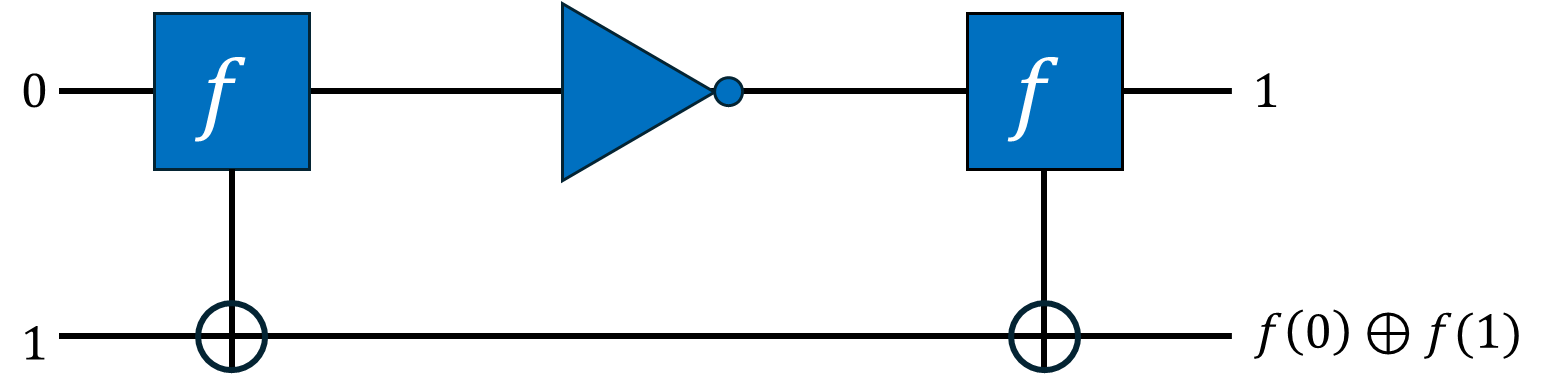
\includegraphics[width=1\linewidth]{../images/Deutsch_classical.png}
    \caption{Classical Deutsch Circuit}
    \label{fig:classical_deutsch}
\end{figure}
The first query XORs the value of $f(0)$ to the second bit. Then the first bit is flipped to 1, so the second query XORs the value of $f(1)$ to the second bit. At the end, the second bit contains the value of $f(0) \oplus f(1)$, which is the solution to Deutsch's problem.



There is an obvious 2-query quantum algorithm that solves the Deutsch's problem just like the circuit shown in the figure \ref{fig:classical_deutsch}.
\section{The Quantum Solution: Deutsch's Algorithm}
\textbf{On a Quantum Computer:}To solve this problem on a Quantum Computer using Deutsch's Algorithm we are required to make only one function call. This speedup is because of the superposition.

Now when we consider the same question in the context of quantum information. We need to change the question slightly, however, in order for it to fit into the model of quantum information that we are considering. More specifically, we must insist that the action of the device corresponds to a unitary transformation. It is therefore not sufficient to consider the black box to be a one qubit action as follows:
\begin{figure}[H]
    \centering
    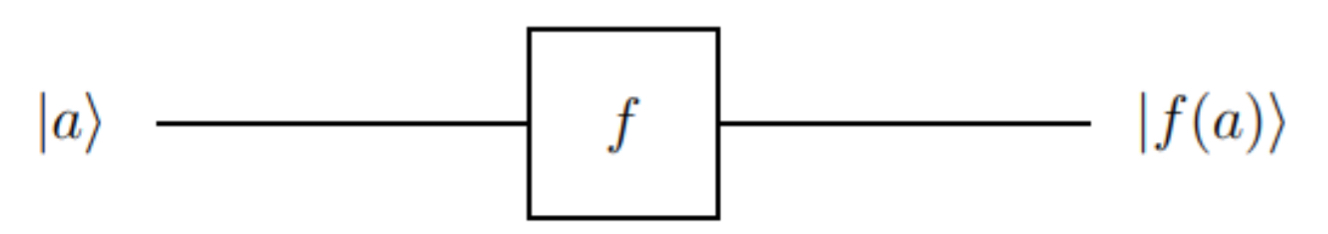
\includegraphics[width=1\linewidth]{../images/Deutsch_bb.png}
    \label{fig:enter-label}
\end{figure}
For example, if $f=f_3$ then this gate would correspond to the matrix
\[
\begin{pmatrix} 1 & 1 \\ 0 & 0 \end{pmatrix}
\]
which is not unitary.

Instead, for any function $f:\{0,1\}\rightarrow\{0,1\}$ we define a 2-qubit quantum gate $B_f$ as follows:
\begin{figure}[H]
    \centering
    \includegraphics[width=1\linewidth]{../images/deutsch_oracle.png}
    \caption{Oracle}
    \label{fig:deutsch_oracle}
\end{figure}
It can be verified that the corresponding matrix is unitary for and function $f$. For example, if $f=f_4$ from the table \ref{tab:Deutsch}, then $f(0_=1$ and $f91)=0$, so the corresponding matrix is
\[
\begin{pmatrix} 0 & 1 & 0 & 0 \\1 & 0 & 0 & 0\\ 0 & 0 & 1 & 0 \\ 0 & 0 & 0 & 1 \end{pmatrix}
\]
For any function $f$, the matrix corresponding to $B_f$ will always be a permutation matrix, meaning that all of the entries are 0 or 1 and every row and every column has exactly one 1 in it. Permutation matrices are always unitary.

In general, if
\[
f:\{0,1\}^n\rightarrow \{0,1\}^m
\]
is any function (for any positive integers n and m).. The associated quantum transformation $B_f$ will be defined by
\[
B_f\ket{x}\ket{y}=\ket{x}\ket{y\oplus f(x)}
\]
(where $\oplus$ denotes the bitwise exclusive OR). The associated matrix will always be a permutation matrix, and is therefore unitary. Note that we generally assume the second input to the oracle to be $\ket{0}$ so this simplifies the oracle to as follows:
\[
B_f\ket{x}\ket{0}=\ket{x}\ket{0 \oplus f(x)}=\ket{x}\ket{f(x)}
\]

The circuit for Deutsch's Algorithm is as shown in the figure \ref{fig:deutsch}.
\begin{figure}[H]
    \centering
    \includegraphics[width=1\textwidth]{../images/deutsch.png}
    \caption{Deutsch's Algorithm}
    \label{fig:deutsch}
\end{figure}
Consider the oracle as shown in the figure \ref{fig:deutsch}. The oracle is a black box which takes inputs $\ket{x}$ and $\ket{y}$ as inputs 
and outputs $\ket{x}$ and $\ket{y\oplus f(x)}$ as outputs. It is a unitary operator (denoted by $U_f$) and implements the functions $f$.

\subsection{Idea of the Algorithm}
The primary limitation of the classical algorithm is that we can either input 0 or 1 to the reversible classical query. It is the because of this classical limitation imposed by the classical laws of physics that does not allow us to compute the solution in one single query but requires two separate queries. This classical limitation is overcome in case of quantum solution. The input to the black-box/quantum query model of computation can be a superposition of 0 and 1 and thus allows simultaneous computation of both the inputs 0 and 1 to the function. Then using some manipulations, upon measurement we can get a distinctive results which can results in clearly distinguished two classical outcomes either 0 or 1 thus allowing us to identify whether the function $f$ was constant or balanced. It is the power of superposition of states of 0 and 1 in application of the laws quantum mechanics and thus quantum computing that allows us to identify the function $f$ in a single query.

\subsection{Algorithm}
\textbf{Claim: }If upon measurement of the first qubit, if it is $\ket{0}$ then the function is constant or else the function is balanced.
\\
\textbf{Analysis: }At inputs both the qubits $q_0=\ket{0}$ and $q_1=\ket{0}$. As $q_0$ passes though the Hadamard Gate it becomes $\ket{+}=\frac{\ket{0}+\ket{1}}{\sqrt{2}}$.
As the qubit $q_1$ passes through X gate, its output is $\ket{1}$ and then it is passed through H gate thus, its state at the output of the Hadamard gate will be $\ket{-}= \frac{\ket{0}-\ket{1}}{\sqrt{2}}$.
thus, at the oracle we have $\ket{+}$ and $\ket{-}$ as inputs. Thus, the action of oracle is:
\[
    U_f\ket{x}\ket{y}=\ket{x}\ket{y\oplus f(x)}
\]
Thus, the action of oracle will be as follows:
\begin{align*}
    U_f\ket{+}\ket{-}&=U_f(\frac{\ket{0}+\ket{1}}{\sqrt{2}}\frac{\ket{0}-\ket{1}}{\sqrt{2}})\\
    U_f\frac{1}{2}\left(\ket{00}-\ket{01}+\ket{10}-\ket{11}\right)&=\frac{1}{2}\left[\ket{0}\ket{0\oplus f(0)}-\ket{0}\ket{1\oplus f(0)}+\ket{1}\ket{0\oplus f(1)}-\ket{1}\ket{1\oplus f(1)}\right]
\end{align*}
Thus, the output of the oracle is as shown above.
Now consider two cases:
\begin{enumerate}
    \item \textbf{Case 1: Function is Constant $f(0)=f(1)=0$}\\
    If the function is constant then $f(0)=f(1)$. Let $f(0)=f(1)=0$ and thus the output of the oracle will be:
    \[
        \frac{1}{2}\left[\ket{0}\ket{0}-\ket{0}\ket{1}+\ket{1}\ket{0}-\ket{1}\ket{1}\right]
    \]
    Now factorizing the above into tensor product of two states as:
    \[
        \frac{1}{2}\left[\ket{0}\ket{0}-\ket{0}\ket{1}+\ket{1}\ket{0}-\ket{1}\ket{1}\right]=\frac{\ket{0}+\ket{1}}{\sqrt{2}}\otimes \frac{\ket{0}-\ket{1}}{\sqrt{2}}
    \]
    \[
        (H\otimes I)(\ket{+} \otimes \ket{-})=\ket{0}\otimes \ket{-}
    \]
    Hence, as the qubit $q_0$ passes through the Hadamard gate, the action of the Hadamard gate on the first qubit will be $H\ket{+}=\ket{0}$. 
    Thus, upon measurement the output will be $\ket{0}$ with probability $1$. Thus, we get a measurement of 0.
    
    \item \textbf{Case 1: Function is Constant $f(0)=f(1)=1$}\\
    If the function is constant then $f(0)=f(1)$. Let $f(0)=f(1)=1$ and thus the output of the oracle will be:
    \[
        \frac{1}{2}\left[\ket{0}\ket{1}-\ket{0}\ket{0}+\ket{1}\ket{1}-\ket{1}\ket{0}\right]
    \]
    Now factorizing the above into tensor product of two states as:
    \[
        \frac{1}{2}\left[\ket{0}\ket{1}-\ket{0}\ket{0}+\ket{1}\ket{1}-\ket{1}\ket{0}\right]=\frac{\ket{0}+\ket{1}}{\sqrt{2}}\otimes -\left(\frac{\ket{0}-\ket{1}}{\sqrt{2}}\right)
    \]
    \[
        (H\otimes I)(\ket{+} \otimes -\ket{-})=\ket{0}\otimes -\ket{-}
    \]
    Hence, as the qubit $q_0$ passes through the Hadamard gate, the action of the Hadamard gate on the first qubit will be $H\ket{+}=\ket{0}$.
    Thus, upon measurement the output will be $\ket{0}$ with probability $1$. Thus, we get a measurement of 0.
    
    \item \textbf{Case 2: Function is Balanced with $f(0)=0$ and $f(1)=1$}\\
    If the function is balanced then $f(0)\neq f(1)$ and let $f(0)=0$ and $f(1)=1$. Thus, the output of the oracle will be:
    \[
        \frac{1}{2}\left[\ket{0}\ket{0}-\ket{0}\ket{1}+\ket{1}\ket{1}-\ket{1}\ket{0}\right]
    \]
    Now factorizing the above into tensor product of two states as:
    \[
        \frac{1}{2}\left[\ket{0}\ket{0}-\ket{0}\ket{1}+\ket{1}\ket{1}-\ket{1}\ket{0}\right]=\frac{\ket{0}-\ket{1}}{\sqrt{2}}\otimes \frac{\ket{0}-\ket{1}}{\sqrt{2}}
    \]
    \[
        (H\otimes I)(\ket{-} \otimes \ket{-})=\ket{1}\otimes \ket{-}
    \]
    Hence, as the qubit $q_0$ passes through the Hadamard gate, the action of the Hadamard gate on the first qubit will be $H\ket{-}=\ket{1}$.
    Thus, upon measurement the output will be $\ket{1}$ with probability $1$. Thus, we get a measurement of 1.

    \item \textbf{Case 2: Function is Balanced with $f(0)=1$ and $f(1)=0$}\
    If the function is balanced then $f(0)\neq f(1)$ and let $f(0)=1$ and $f(1)=0$. Thus, the output of the oracle will be:
    \[
        \frac{1}{2}\left[\ket{0}\ket{1}-\ket{0}\ket{0}+\ket{1}\ket{0}-\ket{1}\ket{1}\right]
    \]
    Now factorizing the above into tensor product of two states as:
    \[
        \frac{1}{2}\left[\ket{0}\ket{1}-\ket{0}\ket{0}+\ket{1}\ket{0}-\ket{1}\ket{1}\right]=\frac{\ket{0}-\ket{1}}{\sqrt{2}}\otimes -\frac{\ket{0}-\ket{1}}{\sqrt{2}}
    \]
    \[
        (H\otimes I)(\ket{-} \otimes -\ket{-})=\ket{1}\otimes -\ket{-}
    \]
    Hence, as the qubit $q_0$ passes through the Hadamard gate, the action of the Hadamard gate on the first qubit will be $H\ket{-}=\ket{1}$.
    Thus, upon measurement the output will be $\ket{1}$ with probability $1$. Thus, we get a measurement of 1.
\end{enumerate}
Note that we can summarise the above results as shown. Recall that the output from the oracle was
\begin{align*}
&\frac{1}{2}\left[\ket{0}\ket{0\oplus f(0)}-\ket{0}\ket{1\oplus f(0)}+\ket{1}\ket{0\oplus f(1)}-\ket{1}\ket{1\oplus f(1)}\right]\\
&\frac{1}{2}[\ket{0}\left(\ket{0\oplus f(0)}-\ket{1\oplus f(0)}\right) + \ket{1}\left(\ket{0 \oplus f(1)} - \ket{1 \oplus f(1)} \right)]
\end{align*}
Now using the fact that 
\[
\ket{0 \oplus a}-\ket{1 \oplus a} = (-1)^a(\ket{0}-\ket{1})
\]
we can simplify the above equation to
\[
\frac{1}{2}[\ket{0}(-1)^{f(0)}(\ket{0}-\ket{1}) + \ket{1}(-1)^{f(1)}(\ket{0}-\ket{1})]
\]
which can be further simplified as
\[
\frac{1}{2}[((-1)^{f(0)}\ket{0}+(-1)^{f(1)}\ket{1})(\ket{0}-\ket{1})]
\]
Now factorizing the qubits we get
\[
\left(\frac{1}{\sqrt{2}}((-1)^{f(0)}\ket{0}+(-1)^{f(1)}\ket{1})\right)\otimes \left(\frac{1}{\sqrt{2}}(\ket{0}-\ket{1}\right)
\]
\begin{align*}
&=\left(\frac{1}{\sqrt{2}}((-1)^{f(0)}\ket{0}+(-1)^{f(1)}\ket{1})\right)\otimes \ket{-}\\
&=(-1)^{f(0)}\left(\frac{1}{\sqrt{2}}\ket{0}+\frac{1}{\sqrt{2}}(-1)^{f(0)\oplus f(1)}\ket{1}\right)\otimes \ket{-}
\end{align*}
Now we apply the hadamard gate on the first qubit as shown in the circuit \ref{fig:deutsch}. We get
\begin{align*}
&(H\otimes I)\left(\left(\frac{1}{\sqrt{2}}\ket{0}+\frac{1}{\sqrt{2}}(-1)^{f(0)\oplus f(1)}\ket{1}\right)\otimes (-1)^{f(0)}\ket{-}\right)\\
&=\ket{f(0)\oplus f(1)} \otimes (-1)^{f(0)}\ket{-}
\end{align*}
Here, we have used the observation that
\[
H\left(\frac{1}{\sqrt{2}}\ket{0}+\frac{1}{\sqrt{2}}(-1)^a\ket{1}\right)=\ket{a}
\]
for $a \in \{0,1\}$, which is again easily verified by considering the cases $a=0$ and $a=1$. Thus, upon measurement of the first qubit, the measurement therefore results in the value $f(0) \oplus f(1)$ which is one of the basis states either 0 or 1 with certainty. This value is $0$ if $f$ is constant and $1$ if $f$ is balanced.

In order to summarize the above algorithm, note that in case if the function is constant we get a measurement of 0 and if the function is balanced we get a measurement of 1. Thus, we can determine whether the function is constant or balanced using only one function call. This is a speedup over the classical algorithm which requires two function calls to determine whether the function is constant or balanced.



\section{Deutsch-Josza Algorithm}
This is a generalization of the Deutsch Algorithm.
\begin{definition}
    Given a classical function $f:\{0,1\}^n \rightarrow \{0,1\}$, which takes n input bits and returns a single output bit.
    The function is called constant if $f(x)=0$ or $f(x)=1$ for all $x \in \{0,1\}^n$ and the function is called balanced if $f(x)=0$ for exactly half of the inputs.
\end{definition}

Our aim is to find whether the function $f$ is constant or balanced with as minimum number of queries as possible to the Oracle.

The total number of such possible functions are $2^{2^n}$ out of which $2$ are constant and $\dfrac{2^n!}{2^{n-1}!2^{n-1}!}$ are balanced functions for n input bits and 1 output bit.
Say for the case n=2, the possible functions are as shown in the table \ref{tab:Deutsch-Josza}.
\begin{table}[H]
    \centering
    \begin{subtable}[b]{0.45\linewidth}
        \centering
        \begin{tabular}{|c|c|c|}
            \hline
            Function & Input & Output \\
            \hline
            $f_1$& 00 & 0 \\
            & 01 & 0 \\
            & 10 & 0 \\
            & 11 & 0 \\
            \hline
            $f_2$& 00 & 1 \\
            & 01 & 1 \\
            & 10 & 1 \\
            & 11 & 1 \\
            \hline
        \end{tabular}
        \caption{Constant Function}
    \end{subtable}%
    \begin{subtable}[b]{0.45\linewidth}
        \centering
        \begin{tabular}{|c|c|c|}
            \hline
            Function & Input & Output \\
            \hline
            $f_3$& 00 & 0 \\
            & 01 & 0 \\
            & 10 & 1 \\
            & 11 & 1 \\
            \hline
            $f_4$& 00 & 0 \\
            & 01 & 1 \\
            & 10 & 0 \\
            & 11 & 1 \\
            \hline
            $\vdots$& $\vdots$ & $\vdots$ \\
            \hline
            $f_{9}$ & 00 & 0 \\
            & 01 & 1 \\
            & 10 & 1 \\
            & 11 & 0 \\
            \hline
        \end{tabular}
        \caption{Balanced Function}
    \end{subtable}
    \caption{Possible Functions}
    \label{tab:Deutsch-Josza}
\end{table}

\textbf{On a Classical Computer: }In order to determine whether the function is constant or balanced we need to query the function
for just 1 more than half of the possible inputs. Thus, we require $2^{n-1}+1$ queries to determine whether the function is constant or balanced.
Thus, the time complexity for this on a classical computer is $\mathcal{O}(2^n)$ i.e. exponential time complexity. If all the inputs produce the same output then the function is constant else the function is balanced.

\textbf{On a Quantum Computer: }To solve this problem we need to query the function only once on a Quantum Computer using the Deutsch-Josza Algorithm.
Thus, the time complexity to solve this problem is $\mathcal{O}(1)$ i.e. constant time complexity. This is an exponential speedup over the classical algorithm. The circuit for 
Deutsch Josza Algorithm Circuit is as shown in the figure \ref{fig:deutsch-jozsa}.
\begin{figure}[H]
    \centering
    \includegraphics[width=0.8\textwidth]{../images/Deutsch-Jozsa.png}
    \caption{Deutsch-Josza Algorithm}
    \label{fig:deutsch-jozsa}
\end{figure}
The input of this circuit is $q_0=\ket{0},q_1=\ket{0},q_2=\ket{1}$.
Now at the input we have $\ket{0}^{\otimes n}\ket{1}$ and the action of the Hadamard gate on the input will be:
\[
    H^{\otimes n}\ket{0}^{\otimes n}H\ket{1}=\frac{1}{\sqrt{2^n}}\sum_{x \in \{0,1\}^n}\ket{x}\frac{(\ket{0}-\ket{1})}{\sqrt{2}}
\]
Now the oracle will show the action $U_f$ as $U_f\ket{x}\ket{y}=\ket{x}\ket{y \oplus f(x)}$ and thus the action of the oracle will be:
\begin{align*}
    U_f\left(\frac{1}{\sqrt{2^n}}\sum_{x \in \{0,1\}^n}\ket{x}\frac{(\ket{0}-\ket{1})}{\sqrt{2}}\right)&=U_f\left(\frac{1}{\sqrt{2^n}}\frac{1}{\sqrt{2}}\sum_{x \in \{0,1\}^n}\ket{x}\ket{0}-\ket{x}\ket{1}\right)\\
    &=\frac{1}{\sqrt{2^n}}\frac{1}{\sqrt{2}}\sum_{x \in \{0,1\}^n}U_f\ket{x}\ket{0}-U_f\ket{x}\ket{1}\\
    &=\frac{1}{\sqrt{2^n}}\sum_{x \in \{0,1\}^n}\ket{x}\frac{(\ket{0 \oplus f(x)}-\ket{1\oplus f(x)})}{\sqrt{2}}
\end{align*}
Now $\ket{0 \oplus f(x)}=\ket{f(x)}$ and $\ket{1 \oplus f(x)} = \ket{\overline{f(x)}}$ where $\overline{f(x)}$ is the complement of $f(x)$. Thus, substituting this in the equation we get,
\[
    \frac{1}{\sqrt{2^n}}\sum_{x \in \{0,1\}^n}\ket{x}\frac{(\ket{f(x)}-\ket{\overline{f(x)}})}{\sqrt{2}}
\] 
Now when $f(x)=0$ then $\frac{\ket{f(x)-\ket{\overline{f(x)}}}}{\sqrt{2}}=\frac{\ket{0}-\ket{1}}{\sqrt{2}}=\ket{-}$ and when $f(x)=1$ then $\frac{\ket{f(x)-\ket{\overline{f(x)}}}}{\sqrt{2}}=\frac{\ket{1}-\ket{0}}{\sqrt{2}}=-\ket{-}$.
Thus, this can be written as: 
\[
    \frac{1}{\sqrt{2^n}}\sum_{x \in \{0,1\}^n}\ket{x}\frac{(\ket{f(x)}-\ket{\overline{f(x)}})}{\sqrt{2}}=\frac{1}{\sqrt{2^n}}\sum_{x \in \{0,1\}^n}(-1)^{f(x)}\ket{x}\ket{-}
\]
Now we apply the Hadamard gate on the first n qubits and the action of the Hadamard gate on the first n qubits will be:
\[
    (H^{\otimes n}\otimes I)\left(\frac{1}{\sqrt{2^n}}\sum_{x \in \{0,1\}^n}(-1)^{f(x)}\ket{x}\ket{-}\right)=H^{\otimes n}\left(\frac{1}{\sqrt{2^n}}\sum_{x \in \{0,1\}^n}(-1)^{f(x)}\ket{x}\right)\otimes I\ket{-}
\]
\[
    =\left(\frac{1}{\sqrt{2^n}}\sum_{x \in \{0,1\}^n}(-1)^{f(x)}H^{\otimes n}\ket{x}\right)\otimes \ket{-}
\]
Recall that $H^{\otimes n}\ket{x}=\dfrac{1}{\sqrt{2^n}}\sum_{y \in \{0,1\}^n}(-1)^{x\cdot y}\ket{y}$ for Hadamard gate (refer section \ref{qgate:hadamard}) acting on n qubits. Thus, substituting this in the above equation can be written as:
\[
    \left(\frac{1}{2^n}\sum_{x \in \{0,1\}^n}\sum_{y \in \{0,1\}^n}(-1)^{f(x)+x\cdot y}\ket{y}\right)\otimes \ket{-}
\]
Now, we perform the measurement on the first n qubits. Consider the following two cases:
\begin{enumerate}
    \item \textbf{Case 1: Function is Constant}
    \begin{itemize}
        \item Let $f(x)=0$ for all $x \in \{0,1\}^n$. Hence we need to perform measurement on the first n qubits of the following state:
        \[
            \left(\frac{1}{2^n}\sum_{x \in \{0,1\}^n}\sum_{y \in \{0,1\}^n}(-1)^{x\cdot y}\ket{y}\right)\otimes \ket{-}
        \]
        Upon simplifying we get,
        \[
            \left(\frac{1}{2^n}2^n\ket{0^{\otimes n}}\right)\otimes \ket{-} = \ket{0^{\otimes n}} \otimes \ket{-}
        \]
        Thus, upon measurement the output will be $\ket{0^{\otimes n}}$ with probability $1$. Thus, we get a measurement of $\ket{0^{\otimes n}}$.
        \item Let $f(x)=1$ for all $x \in \{0,1\}^n$. Hence we need to perform measurement on the first n qubits of the following state:
        \[
            \left(\frac{1}{2^n}\sum_{x \in \{0,1\}^n}\sum_{y \in \{0,1\}^n}(-1)^{1+x\cdot y}\ket{y}\right)\otimes \ket{-}
        \]
        Upon simplifying we get,
        \[
            \left(\frac{1}{2^n}2^n\ket{0^{\otimes n}}\right)\otimes \ket{-} = -\ket{0^{\otimes n}} \otimes \ket{-}
        \]
        Thus, upon measurement the output will be $\ket{0^{\otimes n}}$ with probability $1$. Thus, we get a measurement of $\ket{0^{\otimes n}}$.
    \end{itemize}
    \item \textbf{Case 2: Function is Balanced}
    \begin{itemize}
        \item Let $f(x)$ be a balanced function. Thus, $f(x)=0$ for exactly half of the inputs and $f(x)=1$ for the other half of the inputs. Hence we need to perform measurement on the first n qubits of the following state:
        \[
            \left(\frac{1}{2^n}\sum_{x \in \{0,1\}^n}\sum_{y \in \{0,1\}^n}(-1)^{f(x)+x\cdot y}\ket{y}\right)\otimes \ket{-}
        \]
        Upon simplifying we get,
        \[
            \left(\frac{1}{2^n}(2^n)(\pm\ket{11})\right)\otimes \ket{-}=\pm \ket{11}\otimes \ket{-}
        \]
        Depending on the input, for the balanced function the output will either be $\ket{11}$ or $-\ket{11}$.
        In either cases, upon measurement the output will be $\ket{11}$ with probability $1$. Thus, we get a measurement of $\ket{11}$.
    \end{itemize}
\end{enumerate}

\begin{example}
    \begin{figure}[H]
        \centering
        \includegraphics[width=0.8\textwidth]{../images/deutsch-jozsa-algorithm.png}
        \caption{Deutsch-Josza Algorithm for n=2}
        \label{fig:deutsch-jozsaex}
    \end{figure}
    Consider the Deutsch-Josza algorithm for n=2. The possible functions are as shown in the table \ref{tab:Deutsch-Josza}
    and the circuit for the Deutsch-Josza algorithm is as shown in the figure \ref{fig:deutsch-jozsa}. 
    The input to the circuit is $\ket{00}\ket{1}$. The action of the Hadamard gate on the input will be:
    \begin{align*}
        H^{\otimes 2}\ket{00}H\ket{1}&=\frac{1}{2}\sum_{x\in \{0,1\}^2}\ket{x}\frac{\ket{0}-\ket{1}}{\sqrt{2}} \\
        &=\frac{1}{2\sqrt{2}}\left(\ket{000}+\ket{010}+\ket{100}+\ket{110}-\ket{001}-\ket{011}-\ket{101}-\ket{111}\right)
    \end{align*}
    The action of the oracle will be:
    \[
        U_f\left(\frac{1}{2\sqrt{2}}(\ket{000}+\ket{010}+\ket{100}+\ket{110}-\ket{001}-\ket{011}-\ket{101}-\ket{111})\right)=
    \]
    \[
        \frac{1}{2\sqrt{2}}(U_f\ket{000}+U_f\ket{010}+U_f\ket{100}+U_f\ket{110}-U_f\ket{001}-U_f\ket{011}-U_f\ket{101}-U_f\ket{111})
    \]
    \[
    =\frac{1}{2\sqrt{2}}(\ket{00}\ket{f(00)}+\ket{01}\ket{f(01)}+\ket{10}\ket{f(10)}+\ket{11}\ket{f(11)}-\ket{00}\ket{\overline{f(00)}}
    \]
    \[
    -\ket{01}\ket{\overline{f(01)}}-\ket{10}\ket{\overline{f(10)}}-\ket{11}\ket{\overline{f(11)}})
    \]
    Now consider the following cases;
    \begin{enumerate}
        \item \textbf{Case 1: $f(x)$ is constant}\\
        \begin{itemize}
            \item Let $f(x)=0$ for all $x \in \{0,1\}^2$. Thus, the output of the oracle will be:
            \[
                \frac{1}{2\sqrt{2}}(\ket{00}\ket{0}+\ket{01}\ket{0}+\ket{10}\ket{0}+\ket{11}\ket{0}-\ket{00}\ket{1}-\ket{01}\ket{1}-\ket{10}\ket{1}-\ket{11}\ket{1})
            \]
            \[
            =\frac{1}{2\sqrt{2}}(\ket{000}+\ket{010}+\ket{100}+\ket{110}-\ket{001}-\ket{011}-\ket{101}-\ket{111})
            \]
            \[
            =\frac{1}{2}(\ket{00}+\ket{01}+\ket{10}+\ket{11})\otimes \frac{\ket{0}-\ket{1}}{\sqrt{2}}
            \]
            Now we apply Hadamard on the first n qubits and we get:
            \[
                (H^{\otimes 2}\otimes I)\frac{1}{2}((\ket{00}+\ket{01}+\ket{10}+\ket{11})\otimes \ket{-})
            \]
            \[
                =\frac{1}{2}(H^{\otimes 2}\ket{00}+H^{\otimes 2}\ket{01}+H^{\otimes 2}\ket{10}+H^{\otimes 2}\ket{11})\otimes \ket{-}
            \]
            \[
                =\frac{1}{2}[\frac{1}{2}(\ket{00}+\ket{01}+\ket{10}+\ket{11})+\frac{1}{2}(\ket{00}-\ket{01}+\ket{10}-\ket{11})
            \]
            \[
                \frac{1}{2}(\ket{00}+\ket{01}-\ket{10}-\ket{11})+\frac{1}{2}(\ket{00}-\ket{01}-\ket{10}+\ket{11})]\otimes \ket{-}
            \]
            Upon simplifying we get,
            \[
                \frac{1}{4}(4\ket{00})\otimes \ket{-}=\ket{00}\otimes \ket{-}
            \]
            Thus, upon measurement the output will be $\ket{00}$ with probability $1$. Thus, we get a measurement of $\ket{00}$.
            \item Let $f(x)=1$ for all $x \in \{0,1\}^2$. Thus, the output of the oracle will be:
            \[
                \frac{1}{2\sqrt{2}}(\ket{00}\ket{1}+\ket{01}\ket{1}+\ket{10}\ket{1}+\ket{11}\ket{1}-\ket{00}\ket{0}-\ket{01}\ket{0}-\ket{10}\ket{0}-\ket{11}\ket{0})
            \]
            \[
            =\frac{-1}{2\sqrt{2}}(\ket{000}+\ket{010}+\ket{100}+\ket{110}-\ket{001}-\ket{011}-\ket{101}-\ket{111})
            \]
            \[
            =\frac{-1}{2}(\ket{00}+\ket{01}+\ket{10}+\ket{11})\otimes \frac{\ket{0}-\ket{1}}{\sqrt{2}}
            \]
            Now we apply Hadamard on the first n qubits and we get:
            \[
                (H^{\otimes 2}\otimes I)\frac{-1}{2}((\ket{00}+\ket{01}+\ket{10}+\ket{11})\otimes \ket{-})
            \]
            \[
                =\frac{-1}{2}(H^{\otimes 2}\ket{00}+H^{\otimes 2}\ket{01}+H^{\otimes 2}\ket{10}+H^{\otimes 2}\ket{11})\otimes \ket{-}
            \]
            \[
                =\frac{-1}{2}[\frac{1}{2}(\ket{00}+\ket{01}+\ket{10}+\ket{11})+\frac{1}{2}(\ket{00}-\ket{01}+\ket{10}-\ket{11})
            \]
            \[
                \frac{-1}{2}(\ket{00}+\ket{01}-\ket{10}-\ket{11})+\frac{1}{2}(\ket{00}-\ket{01}-\ket{10}+\ket{11})]\otimes \ket{-}
            \]
            Upon simplifying we get,
            \[
                \frac{-1}{4}(4\ket{00})\otimes \ket{-}=-\ket{00}\otimes \ket{-}
            \]
            Thus, upon measurement the output will be $\ket{00}$ with probability $1$. Thus, we get a measurement of $\ket{00}$.
        \end{itemize}
        \item \textbf{Case 2: $f(x)$ is balanced}\\
        \begin{itemize}
            \item Let $f(x)$ be a balanced function. Thus, $f(x)=0$ for exactly half of the inputs and $f(x)=1$ for the other half of the inputs.
            Then it can be shown that based upon the input chosen the output will be either of the first n qubits, $\ket{11}$ or $-\ket{11}$.
            Thus, upon measurement the output will be $\ket{11}$ with probability $1$. Thus, we get a measurement of $\ket{11}$.
        \end{itemize}
    \end{enumerate}
\end{example}
\textbf{Conclusion: }\\
From the above algorithm, we can clearly see that for determining whether the 
function $f:\{0,1\}^n \rightarrow \{0,1\}$ is constant or balanced we need to input the function with n $\ket{0}$ and 1 $\ket{1}$ and query the function only once.
Then, in the final measurement we measure the first n qubits and if the function is constant we get $\ket{0^{\otimes n}}$ and if the function is balanced we get $\ket{11}$.
Thus, we can determine whether the function is constant or balanced with just one query to the Oracle. This is an exponential speedup over the classical algorithm which requires $2^{n-1}+1$ queries to determine whether the function is constant or balanced.
Thus, the time complexity of this algorithm is $\mathcal{O}(1)$ i.e. constant time complexity. Hence, an exponential speedup over the classical algorithm.


\section{Complexity Analysis}
Note that the classical query cost is expensive only if we require absolutely perfect performance. If a classical procedure queries $f$ in random locations then, in case of a balanced function, it would have to be very unlucky to draw the same bit value.

Here's a classical probabilistic procedure that makes just two queries and performs fairly well. It selects two locations randomly (independently) and then outputs "constant" if the two bits are the same and "balanced" if the two bits values are different.

What happens if $f$ is constant? In that case the algorithm always succeeds. What happens if $f$ is balanced? In that case the algorithm succeeds with probability $\frac{1}{2}$. The probability that the two bits will be different will be $\frac{1}{2}$.

By repeating the above procedure k times, we can make the error probability exponentially small with respect to $k$. Only 4 queries are needed to obtain success probability $3/4$. And the success probability can be made to any constant, arbitrarily close to 1, with a constant number of queries.

In summary, we have considered three problems in the black-box model. For each problem, a quantum algorithms solves it with just one query, but more queries are required by classical Algorithm.

\begin{table}[H]
    \centering
    \begin{tabular}{|c|c|c|c|}
    \hline
        Problem & Quantum Solution & Classical Deterministic & Classical Probabilistic\\
        \hline
         Deutsch & 1 & 2 & 2\\
         \hline
         Deutsch-Jozsa & 1 & $2^{n-1}+1$ & $\mathcal{O}(1)$\\
         \hline
    \end{tabular}
    \caption{Summary of Query costs for the problems}
    \label{tab:deutsch_querycost}
\end{table}
For Deutsch's problem, any classical algorithm requires 2 queries. And, for the Deutsch-Jozsa problem, any classical algorithm requires exponentially many queries to solve the problem perfectly. However, there is a probabilistic classical algorithm that makes only a constant number of queries and solves the problem with bounded error probability.

Along this line of thought, the following question seems natural. Is there a black-box problem for which the quantum-vs-classical query cost separation is stronger? For example, for which even probabilistic classical algorithms with bounded-error probability will require exponentially more queries than a quantum algorithm?

We'll address this question in the next chapter.

\section{Implementation using Qiskit}
\subsection{Background}
Usage estimate: 4 seconds (NOTE; This is an estimate only. Your runtime may vary)\\
In order to run Deutsch-Jozsa algorithm (a generalization of Deutsch's algorithm) requires an oracle that implements the function either constant or balanced and Deutsch-Josza Circuit.

Here, we demonstrate how to construct Deutsch-Josza oracles and use the gates from the Qiskit circuit library to easily set up a Deutsch-Josza Circuit. The runtime \textit{Sampler} primitive allows seamless execution of Deutsch-Josza circuit.

\subsection{Requirements}
Before starting this tutorial, enusre that you have the following installed:
\begin{itemize}
    \item Qiskit SDK 1.0 or later, with visualization support ( pip install 'qiskit[visualization]')
    \item Qiskit Runtime (pip install qiskit-ibm-runtime) 0.22 or later
\end{itemize}

\subsection{Setup}
Here we import the small number of tools we need for this tutorial.
\begin{lstlisting}[language=Python]
#Built-in modules
import math

#imports from Qiskit
from qiskit import QuantumCircuit, QuantumRegister, ClassicalRegister
from qiskit.visualization import plot_distribution

#Imports from Qiskit Runtime
from qiskit_ibm_runtime import QiskitRuntimeService
from qiskit_ibm_runtime import SamplerV2 as Sampler
\end{lstlisting}
\begin{lstlisting}[language=Python]
# To run on hardware, select the backend with the fewest number of jobs in the queue
service = QiskitRuntimeService(channel="ibm_quantum")
backend = service.least_busy(operational=True, simulator=False)
backend.name
\end{lstlisting}
This output one of the ibm quantum computers (say 'ibm\_brisbane').
\begin{enumerate}
    \item \textbf{Step 1: Map classical inputs to a quantum problem}: \\
    There are four possibilities for the oracles for the case of Deutsch Circuit where the oracle implements the function $f:\{0,1\}\rightarrow \{0,1\}$ which could either be constant ($f_1$ or  $f_2$) or constant ($f_3$ or $f_4$) as given in table \ref{tab:Deutsch}. The code used for creating the Deutsch Circuit is as follows:
    \begin{lstlisting}[language=Python]
def deutsch_circuit(value):
    # Create a Quantum Circuit
    qubits=QuantumRegister(2,name="q")
    cbits=ClassicalRegister(1,name="c")
    circuit=QuantumCircuit(qubits,cbits)
    
    q0,q1=qubits
    circuit.h(q0)
    circuit.x(q1)
    circuit.h(q1)
    
    circuit.barrier()
    if(value==1):
        circuit.id(q0)
        circuit.id(q1)
    elif(value==2):
        circuit.id(q0)
        circuit.x(q1)
    elif(value==3):
        circuit.cx(q0,q1)
    elif(value==4):
        circuit.cx(q0,q1)
        circuit.x(q1)
    
    circuit.barrier()
    circuit.h(q0)
    
    circuit.measure(q0,0)
    
    return circuit
    \end{lstlisting}
    For creating one of the circuits, use the following code:
    \begin{lstlisting}[language=Python]
        qc_4=deutsch_circuit(value=4)
        qc_4.draw("mpl")
    \end{lstlisting}
    All the circuits along with their corresponding oracles implementing the four functions are as shown in the figure below:
    \begin{figure}[H]
        \centering
        \begin{subfigure}[b]{0.45\linewidth}
        \centering
        \includegraphics[width=1\linewidth]{../images/deutsch_f1.png}
        \caption{$f=f_1$}
        \label{fig:deutsch_f1}
        \end{subfigure}
        \hfill
        \centering
        \begin{subfigure}[b]{0.45\linewidth}
        \centering
        \includegraphics[width=1\linewidth]{../images/deutsch_f2.png}
        \caption{$f=f_2$}
        \label{fig:deutsch_f2}
        \end{subfigure}
        \vspace{0.5 cm}
        \begin{subfigure}[b]{0.45\linewidth}
        \centering
        \includegraphics[width=1\linewidth]{../images/deutsch_f3.png}
        \caption{$f=f_3$}
        \label{fig:deutsch_f3}
        \end{subfigure}
        \hfill
        \begin{subfigure}[b]{0.45\textwidth}
        \centering
        \includegraphics[width=1\linewidth]{../images/deutsch_f4.png}
        \caption{$f=f_4$}
        \label{fig:deutsch_f4}
        \end{subfigure}    
        \caption{Deutsch Circuit implementation for possible functions along with their corresponding oracles}
        \label{fig:deutsch_circuit}
    \end{figure}
    Note that each of the oracle (shown between the two barriers) implements the required function. Thus the above shown figure corresponds to the Deutsch circuit with its functions in the oracle implementation.

    \item \textbf{Step 2: Optimize Problems for Quantum Execution}
\begin{lstlisting}[language=Python]
from qiskit.transpiler.preset_passmanagers import 

generate_preset_pass_manager

target = backend.target
pm = generate_preset_pass_manager(target=target, optimization_level=3)

circuit_isa_1 = pm.run(qc)
circuit_isa_1.draw(output="mpl", idle_wires=False, style="iqp")
\end{lstlisting}

    \begin{figure}[H]
        \centering
        \begin{subfigure}[b]{0.6\linewidth}
        \centering
        \includegraphics[width=1\linewidth]{../images/opt_deutsch_f1.png}
        \caption{$f=f_1$}
        \label{fig:opt_deutsch_f1}
        \end{subfigure}
        \hfill
        \centering
        \begin{subfigure}[b]{0.6\linewidth}
        \centering
        \includegraphics[width=1\linewidth]{../images/opt_deutsch_f2.png}
        \caption{$f=f_2$}
        \label{fig:opt_deutsch_f2}
        \end{subfigure}
        \vspace{0.5 cm}
        \begin{subfigure}[b]{0.6\linewidth}
        \centering
        \includegraphics[width=1\linewidth]{../images/opt_deutsch_f3.png}
        \caption{$f=f_3$}
        \label{fig:opt_deutsch_f3}
        \end{subfigure}
        \hfill
        \begin{subfigure}[b]{0.6\textwidth}
        \centering
        \includegraphics[width=1\linewidth]{../images/opt_deutsch_f4.png}
        \caption{$f=f_4$}
        \label{fig:opt_deutsch_f4}
        \end{subfigure}    
        \caption{Corresponding Optimized Deutsch Circuit}
        \label{fig:opt_deutsch_circuit}
    \end{figure}

    \item \textbf{Step 3: Execute using Qiskit Primitives}\\

    We are now required to run the circuit and sample the measurements on the first qubit. Thus for execution we will use the Sampler runtime primitive.
    \begin{lstlisting}[language=Python]
# TO run on local simulator:
#1. Use the StatevectorSampler from qiskit.primitves instead
sampler=Sampler(backend=backend)
sampler.options.default_shots=10_000
result_1 = sampler.run([circuit_isa_1]).result
dist_1 = result_1[0].data.c.get_counts()   
    \end{lstlisting}
    The output of the above code will be the distribution of the measurements on the first qubit. Similar code can be written for all the four possible functions.

    \item \textbf{Step 4: Post-Process Results}\\
    Now we plot a histogram of the measurements on the first qubit in the classical format.
    \begin{lstlisting}[language=Python]
from qiskit.visualization import plot_histogram
plot_histogram(dist_1)
    \end{lstlisting}
    The output of the above code will be the histogram of the distribution of the measurements on the first qubit. Similar code can be written for all the four possible functions.

    The following output is produced upon running this code on ibm\_brisbane as shown in figure \ref{fig:deutsch_results}. The histogram plot is done for 10000 shots and results can be clearly seen the results as expected. The minor deviations in the results is due to the inherent errors (because of the noise) in the quantum computer and its probabilistic nature in the measurement process.
    \begin{figure}[H]
        \centering
        \begin{subfigure}[b]{0.45\linewidth}
        \centering
        \includegraphics[width=1\linewidth]{../images/deutsch_result_f1.png}
        \caption{$f=f_1 \implies \text{constant}$}
        \label{fig:deutsch_result_f1}
        \end{subfigure}
        \hfill
        \centering
        \begin{subfigure}[b]{0.45\linewidth}
        \centering
        \includegraphics[width=1\linewidth]{../images/deutsch_result_f2.png}
        \caption{$f=f_2\implies \text{constant}$}
        \label{fig:deutsch_result_f2}
        \end{subfigure}
        \vspace{0.5 cm}
        \begin{subfigure}[b]{0.45\linewidth}
        \centering
        \includegraphics[width=1\linewidth]{../images/deutsch_result_f3.png}
        \caption{$f=f_3\implies \text{balanced}$}
        \label{fig:deutsch_result_f3}
        \end{subfigure}
        \hfill
        \begin{subfigure}[b]{0.45\textwidth}
        \centering
        \includegraphics[width=1\linewidth]{../images/deutsch_result_f4.png}
        \caption{$f=f_4\implies \text{balanced}$}
        \label{fig:deutsch_result_f4}
        \end{subfigure}    
        \caption{Results}
        \label{fig:deutsch_results}
    \end{figure}
    We can see in the figure \ref{fig:deutsch_result_f1} that the result of the measurement of the first qubit is 0 (9943 times) and 1 (57 times). Thus, we can conclusively say that the function implemented was a constant function (inside the oracle) which we know is true. Hence, the results are expected. Similar conclusions can be made for all the other results and we can clearly see that they agree with what we implemented and expected.
\end{enumerate}





\chapter{Simon's Algorithm}
\begin{definition}
    Given a function $f:\{0,1\}^n \rightarrow \{0,1\}^n$ which takes n input bits and returns n output bits.
    The function is a two - to - one function, such that $f(x)=f(x\oplus s)$ for $s \in \{0,1\}^n$.
    We are required to find s.
\end{definition}

\begin{example}
    Consider the function $f:\{0,1\}^3 \rightarrow \{0,1\}^3$ for n=3, and let $s=111$. Then, since the function is a two-to-one function i.e. produces the same output for two distinct inputs such that 
    $f(x)=f(x\oplus s)$. Thus, $f(000)=f(000\oplus 111)=f(111), f(001)=f(001\oplus 111)=f(110), f(010)=f(010\oplus 111)=f(101), f(011)=f(011\oplus 111)=f(100), f(100)=f(100\oplus 111)=f(011), f(101)=f(101\oplus 111)=f(010), f(110)=f(110\oplus 111)=f(001), f(111)=f(111\oplus 111)=f(000)$.
    Thus, we have:
    \begin{align*}
        f(000)&=f(111) \\
        f(001)&=f(110) \\
        f(010)&=f(101) \\
        f(011)&=f(100) \\
    \end{align*}
    Consider the fololwing functions as an example with outputs given in tabular form:
    \begin{table}[H]
        \centering
        \begin{tabular}{|c|c|}
            \hline
            Input & Output \\
            \hline
            000 & 111 \\
            001 & 000 \\
            010 & 110 \\
            011 & 010 \\
            100 & 010 \\
            101 & 110 \\
            110 & 000 \\
            111 & 111 \\
            \hline
        \end{tabular}
        \caption{Example of Simon's Algorithm}
        \label{tab:exsimon}
    \end{table}
    It can be clearly seen that the above function is a valid function as it follows the constraints of being a two-to-one function with the above stated constraints.
    We can also clearly see from the table \ref{tab:exsimon} that the function is a two-to-one function and the function is periodic with period $s=111$.
    Thus, its a valid example function for Simon's algorithm.
    Now given that the function is a two-to-one function we are required to find s.
\end{example}

\textbf{On a Classical Computer: }In order to determine the period of the function we need to query the function for $2^{n-1}+1$ times to determine the period of the function.
This is because the total number of possible inputs are $2^n$ and since the function is a two-to-one function with a period of s, it produces the same output for half of the inputs.
Thus, in order to find s calssically, in the worst case scenario we are required to query the function for $2^{n-1}+1$ times to determine the period of the function.
Thus, the time complexity of the algorithm is $\mathcal{O}(2^n)$ i.e. exponential time complexity. So, the best way to solve this problem is using randomized algorithms using some probabilistic approach. In that case, 
the running time is $\mathcal{O}(2^{n/2})$, which is still exponential. Note that once we know two inputs (say x,y) with the same output. Then, we can use $x \oplus y=s$ to find s (because $y=x\oplus s\implies x \oplus y=x\oplus (x \oplus s) = 0\oplus s=s$. Because $x \oplus x=0$).

\textbf{On a Quantum Computer: }To solve this problem we need to query the function $\mathcal{O}(n)$ times on a Quantum Computer using the Simon's Algorithm which is a linear time complexity.
The circuit for Simon's Algorithm is as shown in the figure \ref{fig:simon}.
\begin{figure}[H]
    \centering
    \includegraphics[width=0.4\textwidth]{../images/Simon.png}
    \caption{Simon's Algorithm}
    \label{fig:simon}
\end{figure}

\textbf{Analysis of Simon's Algorithm: }\\
The input to the circuit is $\ket{0}^{\otimes n}\ket{0}^{\otimes n}$. 
Then the action of hadamard gates on the input will be:
\[
(H^{\otimes n} \otimes I^{\otimes n})(\ket{0}^{\otimes n} \otimes \ket{0})=\frac{1}{\sqrt{2^n}}\sum_{x \in \{0,1\}^n}\ket{x}\ket{0}^{\otimes n}
\]
Now the classical function $f$ takes n inputs and produces n outputs and its a two-to-one function with a period s. Thus, in order to implement it on quantum computer, 
we use a quantum oracle $U_f$ which implements the function $f$ as $U_f\ket{x}\ket{y}=\ket{x}\ket{y\oplus f(x)}$.
Here $\ket{y}=\ket{0}^{\otimes n}$, thus the action of the oracle will be $U_f\ket{x}\ket{0}^{\otimes n}=\ket{x}\ket{0 \oplus f(x)}=\ket{x}\ket{f(x)}$.
Thus, the action of the oracle will be:
\[
    U_f\left(\frac{1}{\sqrt{2^n}}\sum_{x \in \{0,1\}^n}\ket{x}\ket{0}^{\otimes n}\right)=\frac{1}{\sqrt{2^n}}\sum_{x \in \{0,1\}^n}\ket{x}\ket{f(x)}
\]
Now  we perform a measurement on the second registers. Now the second registers are in some superposition and upon measurement will 
collapse to some classical values. Let the output of the second register be $f(z)$. Becuase of this the first register will have only those values which are mapped to $f(z)$.

Thus, the state of the system will be:
\[
    \frac{\ket{z}+\ket{z\oplus s}}{\sqrt{2}}\ket{f(z)}
\]
Now applying hadamard gate on the first n qubits will be:
\[
    (H^{\otimes n}\otimes I)\left(\frac{\ket{z}+\ket{z\oplus s}}{\sqrt{2}}\ket{f(z)}\right)=\frac{1}{\sqrt{2}}[(H^{\otimes n}\ket{z}+H^{\otimes n}\ket{z\oplus s})\ket{f(z)}]
\]
\[
    =\frac{1}{\sqrt{2}}[\frac{1}{\sqrt{2^n}}\sum_{y \in \{0,1\}^n}(-1)^{z\cdot y}\ket{y}+\frac{1}{\sqrt{2^n}}\sum_{y \in \{0,1\}^n}(-1)^{(z\oplus s)\cdot y}\ket{y}]\ket{f(z)}
\]
\[
    =\frac{1}{\sqrt{2^{n+1}}}\sum_{y \in \{0,1\}^n}((-1)^{z\cdot y}+(-1)^{(z\oplus s) \cdot y})\ket{y}\ket{f(z)}
\]
\[
    =\frac{1}{\sqrt{2^{n+1}}}\sum_{y \in \{0,1\}^n}(-1)^{z\cdot y}(1+(-1)^{s\cdot y})\ket{y}\ket{f(z)}
\]
Now, there are two possible cases:
\begin{itemize}
    \item \textbf{Case 1: $y\cdot s=1$}. Then the amplitude of y will be zero and thus that value won't be taken in the superposition.
    \item \textbf{Case 2: $y\cdot s=0$}.Then the amplitude of that corresponding y will be 2 and thus will be in the superposition.
\end{itemize}
Thus, the supoerposition will consist of only those values of y for which $y\cdot s=0$.
We can use this fact to run the circuit n times and attain a system of n linearly independent equations. We can then solve these equations to find s.
\begin{example}
    Consider the function $f:\{0,1\}^4\rightarrow \{0,1\}^4$ as shown in the table \ref{tab:simonex2}.
    \begin{table}[H]
        \centering
        \begin{tabular}{|c|c|}
            \hline
            Input & Output \\
            \hline
            0000,1001 & 1111 \\
            0001, 1000 & 0001 \\
            0010,1011 & 1110 \\
            0011,1010 & 1101 \\
            0100,1101 & 0000 \\
            0101,1100 & 0101 \\
            0110,1111 & 1010 \\
            0111,1110 & 1001 \\
            \hline
        \end{tabular}
        \caption{Function}
        \label{tab:simonex2}
    \end{table}
    Here, $s=1001$. Now, say the above shown function has been implemented in a quantum oracle. We are required to find s for the function using Simon's algorithm.

    Now at the input the state of the system will be:
    \[
        \ket{0^4}\ket{0^4}=\ket{0000}\ket{0000}
    \]
    Now we apply hadamard gate on the first register. Thus, the state of the system will now be:
    \[
        (H^{\otimes 4} \otimes I^{\otimes 4})(\ket{0000}\otimes \ket{0000})=\frac{1}{\sqrt{2^4}}\sum_{x \in \{0,1\}^4}\ket{x}\ket{0000}
    \]
    \[
        =\left(\frac{1}{4}\sum_{x \in \{0,1\}^4}\ket{x}\right) \otimes \ket{0000}
    \]
    \[
        =\left(\frac{1}{4}\sum_{x \in \{0,1\}^4}\ket{x}\ket{0000}\right)
    \]
    Now, we apply the oracle on the above state ($U_f\ket{x}\ket{y}=\ket{x}\ket{y\oplus f(x)}$). Thus, the state of the system will be:
    \[
    U_f\left(\frac{1}{4}\sum_{x \in \{0,1\}^4}\ket{x}\ket{0000}\right)=\frac{1}{4}\sum_{x \in \{0,1\}^4}U_f\ket{x}\ket{0000}
    \]
    \[
    =\frac{1}{4}\sum_{x\in\{0,1\}^4}\ket{x}\ket{0000 \oplus f(x)}=\frac{1}{4}\sum_{x \in \{0,1\}^4}\ket{x}\ket{f(x)}
    \]
    \[
        \frac{(\ket{0000}\ket{f(0000)}+\ket{0001}\ket{f(0001)}+\ldots +\ket{1110}\ket{f(1110)}+\ket{1111}\ket{f(1111)})}{4}
    \]
    Thus, upon substituting the corresponding values from the table \ref{tab:simonex2} we get, since n=4 we will get 16 terms:
    \begin{align*}
    \frac{1}{4}[\ket{0000}\ket{1111}+\ket{0001}\ket{0001}+\ket{0010}\ket{1110}+\ket{0011}\ket{1101}+\ket{0100}\ket{0000}+\ket{0101}\ket{0101}\\
    \ket{0110}\ket{1010}+\ket{0111}\ket{1001} +\ket{1000}\ket{0001}+\ket{1001}\ket{1111}+\ket{1010}\ket{1101}+\ket{1011}\ket{1110}\\
    +\ket{1100}\ket{0101}+\ket{1101}\ket{0000}+\ket{1110}\ket{1001}+\ket{1111}\ket{1010}]
    \end{align*}
    Now, we perform a measurement on the second register thus the superposition state of the second register will collapse to some classical state. Let the output of the second register be $f(z)$ which comes out as, say $f(z)=1010$.
    Thus, the state of the system now will be only those values which produce $1010$ in the second register as output. Thus, the state of the system will be:
    \[
    \frac{\ket{0110}+\ket{1111}}{\sqrt{2}}\otimes \ket{1010}
    \]
    Now we apply the Hadamard gate on the first register. Thus, the state of the system will be:
    \[
    (H^{\otimes 4}\otimes I^{\otimes 4})(\frac{\ket{0110}+\ket{1111}}{\sqrt{2}}\otimes \ket{1010})
    \]
    Using the property that the Hadamard gate when applied to any input gives $H^{\otimes n}\ket{x}=\frac{1}{\sqrt{2^n}}\sum_{y \in \{0,1\}^n}(-1)^{x\cdot y}\ket{y}$, we get:
    \[
    =\frac{H^{\otimes 4}\ket{0110}+H^{\otimes 4}\ket{1111}}{\sqrt{2}} \otimes \ket{1010}
    \]
    Again applying the general formula for Hadamard gate $H^{\otimes n}\ket{x}=\frac{1}{\sqrt{2^n}}\sum_{y \in \{0,1\}^n}(-1)^{x\cdot y}\ket{y}$, and simplifying (reacll that we are required to consider only those values where $y\cdot s=0$ and the amplitude in that case is 2. For the cases where the $y \cdot s=1$ the amplitude for that corresponding $\ket{y}$ will be zero. Thus,
    we will get only those value where $y\cdot s=0$), we get:
    \[
    \frac{\ket{0000}-\ket{0010}-\ket{0100}+\ket{0110}+\ket{1001}-\ket{1011}-\ket{1101}+\ket{1111}}{\sqrt{2^3}}\otimes \ket{1010}
    \]
    We can also verify that $y \cdot s=0$, (recall that here $s=1001$ and thus, only those terms in the equation survive that have $y\cdot s=0$) using the result from the above. 
    Now when we perform the measurement on the first register we will get one of the above state with equal probability ($=\frac{1}{8}$). 

    Now we are required to get $n-1=4-1=3$ linearly independent y to find s by forming a system of linear equations.
    Say we measure and upon the measurement we get the state $\ket{0000}$. Now state $\ket{0000}$ is a null vector and thus we can't use it to form the system of linear equations.
    
    Now we rerun the circuit and for the next time upon measurement we get, say $\ket{0010}$ which works for the system of linear equations. Thus, our set of vectors for making a linear system 
    of equation contains $\{\ket{0010}\}$.
    
    Now we rerun the circuit and for the next time upon measurement we get, say $\ket{0100}$ which works for the system of linear equations since it is independent of the previous vectors $\ket{0010}$.
    Thus, our set of vectors now contain $\{\ket{0010},\ket{0100}\}$. Now we need one more linearly independent vector to find s.

    Now we rerun the circuit and for the next time upon measurement we get, say $\ket{0110}$ which does not work for the system of linear equations since it is dependent on the previous two vectors ($\ket{0110}$ can be made using $0100 \oplus 0010 = 0110$).

    Now we rerun the circuit and for the next time upon measurement we get, say $\ket{1001}$ which works for the system of linear equations since it is independent of the previous vectors $\ket{0010}$ and $\ket{0100}$.
    Thus, our set of vectors now contains $\{\ket{0010},\ket{0100},\ket{1001}\}$. Now we have 3 linearly independent vectors and thus we can form a system of linear equations to find s.

    Now, we know that each of the linearly indpendent vector in the set $\{\ket{0010},\ket{0100},\ket{1001}\}$ is a solution to the equation $y\cdot s=0$. Thus, we can form a system of linear equations as shown below:
    \[
    \begin{bmatrix}
        0 & 0 & 1 & 0 \\
        0 & 1 & 0 & 0 \\
        1 & 0 & 0 & 1 \\
        0 & 0 & 0 & 0
    \end{bmatrix}
    \begin{bmatrix}
        s_1 \\
        s_2 \\
        s_3 \\
        s_4 
    \end{bmatrix}
    =
    \begin{bmatrix}
        0 \\
        0 \\
        0 \\
        0
    \end{bmatrix}
    \]
    Upon, solving this system of lienear equations we get:
    \begin{align*}
    s_3&=0 \\
    s_2&=0 \\
    s_1 + s_4 &=0 \\
    \end{align*}
    Now, we can choose one of the values of $s_1$ or $s_4$. Let us choose $s_4$.
    Now, $s_4=0$ or $s_4=1$. 
    Let us choose $s_4=0$ then we get, $s_1=0$ which gives a trivial solution os $s=0000$. Let $s_4=1$ then we get, $s_1=-1\implies (-1) mod 2=1$.
    Thus, we get $s=1001$ which is the correct solution.
\end{example}


\section{Bernstein-Vazirani Algorithm}

\section{Shor's Algorithm}
\begin{definition}
    Given a number $N$ which is a composite number. We are required to find the prime factors of the number $N$.
\end{definition}

\chapter{Grover's Search Algorithm}
It is the second most famous quantum algorithm after Shor's algorithm.
It doesn't prove exponential speed up, but only a quadratic speedup, yet it is much more
widely applicable than Shor's algorithm.

\section{The Problem Definition}
\begin{definition}
    \textbf{The Search Problem} For $N = 2^n$, we are given an arbitrary $x \in \{0, 1\}^n$.
    Suppose we have a function
    \[
        f:\{0,1\}^n \rightarrow \{0,1\}
    \]
    that is implemented by a reversible transformation (Oracle) $B_f$ in the usual way:
    \[
        B_f\ket{x}\ket{a}=\ket{x}\ket{a\oplus f(x)}
    \]
    for all $x \in \{0,1\}^n$ and $a \in \{0,1\}$. (We can build a quantum circuit for $B_f$ given a Boolean circuit for $f$ at a cost linear in size of boolean circuit). The problem of search is to simply find a string 
    $ x \in \{0,1\}^n$ such that $f(x)=1$, or to conclude that no such $x$ exists if $f$ is identically 0. 

    This is also called as unstructured search problem because f is arbitrary i.e. there is no promise and we can't rely on it have a structure that makes finding solutions easy.
    \begin{remark}Here, we assume that the we can easily evaluate this function $f$ (function can be computed efficiently). That is, maybe we have a boolean circuit whose size is poly(n). This does not restrict the function to be simple. It can be complex and may not have a simple form. This is a \textit{NP-complete} problem. 
    \end{remark}
\end{definition}

\section{The Classical Solution}
Note that the searching problem is completely unstructured. There are no promises on the function $f$, so it is not possible to use binary search or any 
other fast searching methods to efficiently solve the problem classically. The best classical algorithm for solving the above search problem is Linear search (a \textbf{deterministic algorithm}) and in the worst case it would require $N=2^n$ queries to the black box (to distinguish the case where $f$ is identically 0 from any of the cases where there is a single $x$ for which $f(x)=1$). Thus, $\mathcal{O}(N)$ time complexity. (Here we have assumed that the cost of evaluating $f$ is the one that dominates the computation and hence we talk about the umber of queries to the function $f$ in order to evaluate the time complexity.)

Probabilistically, a best strategy for an algorithm that makes k queries is to simply choose k distinct values of $x$ and to query the black-box at these k values. In the case that there is a single value of x for which $f(x)=1$, and we require that our algorithm succeeds in finding this x with probability at least $1-\epsilon$, then we must have have $1-\frac{k}{2^n}\leq \epsilon$. This implies $k\geq (1-\epsilon)2^n$, so for constant error we need $k=\Omega(2^n)=\omega(N)$ queries to solve the problem.

\textbf{In contrast, the Grover's algorithm will solve the problem using $\mathcal{O}(\sqrt{2^n})$ i.e. $\mathcal{O}(\sqrt{N})$ queries and $\mathcal{O}(\sqrt{N}\log N)$ other gates (the number of gates can be reduced a bit further)}.

\begin{importantnote}
    The problem can be thought of as a table of size N, where exactly one element has value 1, and all others are 0. Searching an item in an unsorted table or array of size N costs a classical computer $\mathcal{O}(N)$ running time. If N is large, this is like searching for a needle in a haystack. This Quantum algorithm for search was proposed by Lov Grover in 1995 that consults the table only $\mathcal{O}(\sqrt{N})$ times.

    In contrast to algorithms like quantum factoring which provide exponential speedups, the search algorithm only provides a quadratic improvement. The same technique used in this algorithm can be used to speedup algorithms for NP-complete problems.

    It is natural to wonder whether there are even faster quantum algorithms for search. However, it turns out that  the quadratic speedup is optimal. This was proved in 1994. Any quantum algorithm for search must consult the table at least some constant times $\sqrt{N}$ times. In this, we have assumed \textit{unique search problem} i.e. This is all assuming that there is only one element that has value 1 and all others have value 0. In case of \textit{multiple solutions} i.e. if there are more than one elements with value 1, then the Grover's algorithm can be modified, and in that case the Complexity becomes $\mathcal{O}(\sqrt{\frac{N}{M}})$, where M is the number of elements with value 1 and N is the total number of elements ($N=2^n)$.
\end{importantnote}
\section{The Quantum Solution: Grover's Algorithm}
Here, we assume the problem to be a Query problem. Thus, the boolean function $f$ implemented on a classical circuit can be converted to a Quantum circuit fro implementing a Query operation using the concepts of reversible computation as explained in section \ref{sec:Oracles}.
\subsection{Idea of the Algorithm}
The best way to describe the Grover's Algorithm is to describe it geometrically. Say we define two sets $A$ and $B$ as follows:
\begin{align*}
A&=\{x\in\{0,1\}^n: f(x)=1\}\\
B&=\{x\in\{0,1\}^n: f(x)=0\}
\end{align*}
Think of $A$ as the set of "good" strings $x \in \{0,1\}^n$; the goal of the algorithm is to find one of these strings. The set $B$ cont contains all of the "bad" strings $x\in\{0,1\}^n$ that do not satisfy the search criterion. Let
\[
a=|A| \quad b=|B|; \quad a+b=N
\]
where $|\cdot|$ denotes cardinality of the sets (i.e. number of elements in the set), with $a\neq 0$ and $b\neq 0$ (The case with $a=0$ or $b=0$ will be considered separately). Although the analysis is for the general case, it might be easier to imagine an interesting case of the problem where a is very small (say $a=1$) and therefore $b$ is very large (close to $N=2^n$, say $b=N-1$). Note that for each $x \in \{0,1\}^n$ it will be either in $A$ or in $B$ but not both since the output corresponding to the input to the function is either 0 or 1. Thus, an arbitrary $x$ will be either in $A$ or in $B$. In other words, the sets A and B are mutually exclusive sets.
Next we define, 
\begin{align*}
    \ket{A}&=\frac{1}{\sqrt{a}}\sum_{x\in A} \ket{x}\\
    \ket{B}&=\frac{1}{\sqrt{b}}\sum_{x \in B} \ket{x}
\end{align*}
which means $\ket{A}$ is the superposition of all the input states to the function $f$ which yield output 1 and similarly, $\ket{B}$ is the superposition of all the input states to the function $f$ which output 0. Now since sets A and B were mutually exclusive and each $x$ lies either in A or B. Clearly $\ket{A}$ and $\ket{B}$ are orthogonal i.e. $\braket{A|B}=0$ because each of the basis state $\ket{x}$ is either in A or in B, thus its corresponding component in the other set is 0, thus their inner product will result in 0. Hence, $\ket{A}$ and $\ket{B}$ are orthogonal. 

The two vectors $\ket{A}$ and $\ket{B}$ form a two-dimensional subspace geometrically. Now consider an equal superposition state of all the possible $\ket{x}$ i.e. $\ket{h}=\frac{1}{\sqrt{N}}\sum_x\ket{x}$. Note that the two-dimensional subspace formed by the two orthogonal vectors $\ket{A}$ and $\ket{B}$ contains $\ket{h}$ i.e. $\ket{h}$ can be expressed as a linear combination of the basis vectors of the two-dimensional subspace as follows:
\begin{align*}
\ket{h}&=\frac{1}{\sqrt{N}}\sum_x\ket{x}\\
&=\frac{1}{\sqrt{N}}\left(\sum_{x\in A}\ket{x}+\sum_{x\in B}\ket{x}\right)\\
&=\frac{\sqrt{a}}{\sqrt{N}}\frac{1}{\sqrt{a}}\sum_{x\in A}\ket{x} + \frac{\sqrt{b}}{\sqrt{N}}\frac{1}{\sqrt{b}}\sum_{x\in B}\ket{x}\\
\ket{h}&=\frac{\sqrt{a}}{\sqrt{N}}\ket{A}+\frac{\sqrt{b}}{\sqrt{N}}\ket{B}
\end{align*}
Considering for the purpose of imagination one could think of $a<<b$ so that the search problem is like finding a needle in a haystack. In pother words, the component of $\ket{h}$ on $\ket{A}$ is much smaller than the component of $\ket{h}$ on $\ket{B}$. Thus, geometrically in space one could imagine this as $\ket{h}$ being very close to $\ket{B}$ then $\ket{A}$ as depicted in the following figure \ref{fig:geometry}
\begin{figure}[H]
    \centering
    \includegraphics[width=0.5\linewidth]{../images/grover.png}
    \caption{Geometric Visualization}
    \label{fig:geometry}
\end{figure}
In the figure \ref{fig:geometry} it can be clearly seen that the$\ket{A}$ and $\ket{B}$ are orthogonal. Say $X=\ket{h}$ makes an angle $\theta$ with $\ket{B}$ (Note that for the purpose of easier imagination as said in the case where $a<<b$, (say $a=1, b=N-1$) which is mostly the case, i.e. when the number of good strings to be searched for is much less than the bad strings, the component of $\ket{h}$ on $\ket{A}$ ($=\frac{\sqrt{a}}{\sqrt{N}}$) will be much less than the component of $\ket{B}$ on $\ket{h}$ ($=\frac{\sqrt{b}}{\sqrt{N}}$) since $a<<b$. Thus, as shown in the figure \ref{fig:geometry}, $\ket{h}$ is much closer to $\ket{B}$ than $\ket{A}$.) 

Note that it is easy to create the state $\ket{h}$ since it is simply an equal superposition of all the states. Thus can be created by applying $H^{\otimes n}$ to $\ket{0^n}$. From figure \ref{fig:geometry} we are required to make a series of rotations/unitary transformations such that eventually $\ket{h}$ gets closer to $\ket{A}$ (or becomes $\ket{A}$), thus achieving the purpose of finding the superposition of strings $x \in \{0,1\}^n$ whose input to the function yields output 1. Then, upon measurement of this state we get one of the required strings whose input to the function yields output 1.

The Unitary transformations (recall that they are simply rotations or reflections in the complex Plane i.e. Hilbert Space) required to perform this are a series of reflections as follows (Starting with $\ket{X}=\ket{h}$):
\begin{enumerate}
    \item Reflect $X$ about $\ket{B}$ which as shown in the figure \ref{fig:geometry} becomes $\ket{X'}$. Say this is denoted by the Unitary matrix $R_{\ket{B}}$. Thus, $\ket{X'}=R_{\ket{B}}\ket{X}$
    \item Now reflect $\ket{X'}$ about $X$ which as shown in the figure \ref{fig:geometry} becomes $\ket{X''}$. Say this is denoted by the Unitary matrix $R_{\ket{X}}$. Thus, $\ket{X''}=R_{\ket{X}}\ket{X'}$
\end{enumerate}
After each iteration we put $\ket{X}=\ket{X''}$ and repeat the above two steps.
Thus, the angle of $\ket{X''}$ with $\ket{B}$ is $3\theta$ after doing this reflections for the first time.
Hence, the $\ket{X''}$ obtained in the second step is now clearly closer to $\ket{A}$. Thus, performing the above steps repeatedly will bring the $\ket{X}$ closer and closer to $\ket{A}$ with each iteration as it moves farther and farther from $\ket{B}$. Once the state $\ket{X''}$ is close enough to $\ket{A}$, measuring the state will result in the required search string with a very high probability.
Thus, till now what we have done is the following:
\[
\ket{0^n}\xrightarrow{H^{\otimes n}} \ket{h}
\]
Then we repeat the following unitary transformation a finite number of times ($\mathcal{O}(\sqrt{N})$ times) starting with $\ket{X}=\ket{h}$
\[
\ket{X} \xrightarrow{R_{\ket{B}}} \ket{X'} \xrightarrow{R_{\ket{X}}} \ket{X''}
\]
Then, finally we make a measurement on $\ket{X''}$ (since it gets very close to A as shown above) and the result of that measurement is one the strings whose input to the function yields output 1. Thus, the required algorithm. This is the idea behind the Grover's algorithm.
It would suffice if we could find the two unitary transformation matrices corresponding to the reflections and show that it does perform the task of reflection about $\ket{B}$ and reflection about $\ket{X}$ respectively and along with that we are required to find the optimal number of times to repeat the process. All of this is answered in the next section.

\subsection{Algorithm}
\subsubsection{Reflection about $\ket{B}$} 
Recall that $\ket{h}$ can be written as linear superposition of the basis $\ket{A}$ and $\ket{B}$ as follows (where both $\ket{A}$ and $\ket{B}$ are orthogonal):
\[
\ket{h}=\frac{\sqrt{a}}{\sqrt{N}}\ket{A}+\frac{\sqrt{b}}{\sqrt{N}}\ket{B}
\]
In order to reflect $\ket{h}$ about $\ket{B}$, see figure \ref{fig:geometry}, we are required to reverse the component of projection of $\ket{h}$ on $\ket{A}$. Thus, the reflected vector should have the following linear superposition:
\[
\ket{X'}=-\frac{\sqrt{a}}{\sqrt{N}}\ket{A}+\frac{\sqrt{b}}{\sqrt{N}}\ket{B}
\]
In other words, all we need to do is flip the phase of the component in the direction of $\ket{A}$. For a general $\ket{X}$  which arises in some intermediate step of the iteration, (which will be a linear superposition of $\ket{A}$ and $\ket{B}$) we are required to reverse the phase on the components in the direction of $\ket{A}$ keeping the components in the direction of $\ket{B}$ unchanged. In order to achieve this, we use \textbf{Phase Query Gate}. Consider the following unitary transformation on n qubits:
\[
Z_f\ket{x}=(-1)^{f(x)}\ket{x}
\]
This is also called a \textit{phase kickback}. This transformation would take in the superposition state and reverse the phase of only those components which are in $\ket{A}$ (i.e. whose $f(x)=1$) using linearity property of distributive action of a matrix on sum of vectors (superposition state). We now study the corresponding circuit as shown in the figure \ref{fig:reflect_about_b} which performs this transformation.
\begin{figure}[H]
    \centering
    \includegraphics[width=1\linewidth]{../images/reflect_about_b.png}
    \caption{Reflection about B circuit}
    \label{fig:reflect_about_b}
\end{figure}
Here, recall that the transformation $B_f$ is the quantum implementation of the classical function $f$ i.e. $B_f\ket{x}\ket{y}=\ket{x}\ket{y\oplus f(x)}$.
We now analyse the circuit. The input to the circuit is $\ket{x}\ket{0}$. Here $\ket{0}$ is the ancilla bit. We then apply NOT-gate on the second register:
\[
\ket{x}\ket{0}\xrightarrow{I^{\otimes n}\otimes X}\ket{x}\ket{1}
\]
Then we apply a Hadamard gate on the output on the second register, thus we get,
\[
\ket{x}\ket{1}\xrightarrow{I^{\otimes n}\otimes H}\ket{x}\frac{\ket{0}-\ket{1}}{\sqrt{2}}
\]
Now we use the Oracle $B_f$ on this,
\[
B_f\ket{x}\frac{\ket{0}-\ket{1}}{\sqrt{2}}=\frac{1}{\sqrt{2}}B_f\ket{x}\ket{0}-\frac{1}{\sqrt{2}}B_f\ket{x}\ket{1}=\frac{1}{\sqrt{2}}\ket{x}\ket{0\oplus f(x)}-\frac{1}{\sqrt{2}}\ket{x}\ket{1\oplus f(x)}
\]
This can be further simplified as follows:
\[
\frac{1}{\sqrt{2}}\ket{x}\ket{f(x)}-\frac{1}{\sqrt{2}}\ket{x}\ket{\overline{f(x)}}=\ket{x}\frac{\ket{f(x)}-\ket{\overline{f(x)}}}{\sqrt{2}}=(-1)^{f(x)}\ket{x}\frac{\ket{0}-\ket{1}}{\sqrt{2}}
\]
Then we perform the uncomputation on the second register by applying a Hadamard gate and then a NOT gate as shown in the figure \ref{fig:reflect_about_b}.
\[
(-1)^{f(x)}\ket{x}\frac{\ket{0}-\ket{1}}{\sqrt{2}}\xrightarrow{I^{\otimes n}\otimes H}(-1)^{f(x)}\ket{x}\ket{1}\xrightarrow{I^{\otimes n}\otimes X}(-1)^{f(x)}\ket{x}\ket{0}
\]
Now, ignoring the ancilla bit we have thus achieved the following transformation
\[
Z_f\ket{x}=(-1)^{f(x)}\ket{x}
\]
which was the required transformation for the reflection of $\ket{X}$ over $\ket{B}$ done by reversing the phase of the components in the direction of $\ket{A}$. Note that we were required to perform one evaluation of $B_f$ implemented in $X_f$ to reflect about $\ket{B}$. Thus, what we have achieved through this Oracle as a Unitary operator can be seen from the fact that consider a $\ket{X}$ as some linear superposition of $\ket{A}$ and $\ket{B}$ (recall, $\ket{A}$ and $\ket{B}$ are orthogonal and $\ket{X}$ lies in the two-dimensional subspace spanned by $\ket{A}$ and $\ket{B}$) , say $\ket{X}=r\ket{A}+s\ket{B}$ for some $r,s$. Then upon applying the operator/Oracle $Z_f$ on this $\ket{X}$ we get,
\begin{align*}
Z_f\ket{X}&=r Z_f\ket{A}+r Z_f\ket{B}\\
&=r Z_f\frac{1}{\sqrt{a}}\sum_{x\in A}\ket{x}+s Z_f\frac{1}{\sqrt{b}}\sum_{x\in B}\ket{x}\\
&=r \frac{1}{\sqrt{a}}\sum_{x\in A}Z_f\ket{x}+s \frac{1}{\sqrt{b}}\sum_{x\in B}Z_f\ket{x}\\
&=r \frac{1}{\sqrt{a}}\sum_{x\in A}-\ket{x}+s \frac{1}{\sqrt{b}}\sum_{x\in B}\ket{x}\\
&=-r \ket{A}+s\ket{B}
\end{align*}
As can be seen that the component of $\ket{X}$ along $\ket{A}$ is reversed. Thus, we achieve the reflection about $\ket{B}$.

\subsubsection{Reflection about $\ket{X}$}
For the reflection about $\ket{X}$, we use the 
Diffusion operator $D$ (assume $N=2^n$), 
which works as follows. 
First, apply $H^{\otimes n}$, which maps 
$\ket{X}\rightarrow \ket{00\ldots 0}$. 
then reflect around $\ket{00\ldots 0}$ this 
is accomplished by the circuit $U_g$, where $g$ 
is a function such that $g(00\ldots 0)=0$ and $g(x)=1$ 
for $x \neq 00\ldots 0$. Finally, apply $H^{\otimes n}$ 
to return to the original basis. (Note that this is simply 
a reflection around the zero vector in the Hadamard basis). 
This is the general idea of Reflection about $\ket{X}$. 
In order to understand this operation better we get into 
the details as follows.
Consider an operator $Z_0$ as follows:
\[
Z_0=I-2\ket{0^n}\bra{0^n}
\]
Thus,
\[
D=H^{\otimes n}Z_0H^{\otimes n}=H^{\otimes n}(I-2\ket{0^n}\bra{0^n})H^{\otimes n}=I-2\ket{h}\bra{h}
\]
This is also the same as having a phase query gate $Z_{OR}$ ($=-Z_0$) for the n-bit OR function:
\[
OR(x)=\begin{cases}
    0, \quad x=0^n \\ 1, \quad x\neq0^n
\end{cases}
\]
for all $x \in \{0,1\}^n$.
\[
Z_{OR}(x)=\begin{cases}
    \ket{x} \quad x=0^n \\
    -\ket{x} \quad x\neq0^n
\end{cases}
\]
for all $x \in \{0,1\}^n$. Note that $Z_{OR}=-Z_0=2\ket{0^n}\bra{0^n}-I$. Note that this does not depend on function $f$ and thus requires no queries. To implement this on a quantum circuit we convert the classical implementation of a n-bit OR boolean circuit.
We now make the following propositions:
\begin{proposition}
    The Diffusion operator D has two properties:
    \begin{enumerate}
        \item It is Unitary and can be efficiently realised.
        \item It can be seen as an "inversion about the mean".
    \end{enumerate}
\end{proposition}
\begin{proof}
    \begin{enumerate}
        \item To prove that D is unitary it suffices to prove that $H^{\otimes n}$ and $Z_0$ is Unitary. Clearly, $H^{\otimes n}$ is unitary since it is a Hadamard Gate tensored product n times. Now for proving that $Z_0$ is unitary. We do as follows:
        \begin{align*}
        Z^{\dagger}_0&=(I-2\ket{0^n}\bra{0^n})^{\dagger}\\
        &=I^{\dagger}-2(\ket{0^n}\bra{0^n}^{\dagger}\\
        &=I-2\ket{0^n}\bra{0^n}=Z_0\\
        \end{align*}
        Thus, $Z_0$ is Hermitian. Now doing $Z^{\dagger}_0Z_0$, we get,
        \begin{align*}
        Z^{\dagger}Z_0=Z_0Z^{\dagger}_0&=(I-2\ket{0^n}\bra{0^n})(I-2\ket{0^n}\bra{0^n})\\
        &=I-2\ket{0^n}\bra{0^n}-2\ket{0^n}\bra{0^n}+4\ket{0^n}\bra{0^n}\\
        &=I
        \end{align*}
        Thus, $Z_0$ is Unitary. Hence $D=H^{\otimes n}Z_0H^{\otimes n}$ is a product of Unitary matrices and hence itself is a Unitary Matrix. Observe that D is expressed as the product of three Unitary matrices (two hadamard Matrices separated by a conditional phase shift matrix). Therefore, D is also Unitary. regarding the implementation, both the Hadamard and the conditional phase shift transforms can be efficiently realized within $\mathcal{O}(n)$ gates.
        \item Consider $D$ operating on a vector $\ket{\alpha}$ to generate another vector $\ket{\beta}$.
        \[
        D\begin{bmatrix}\alpha_1 \\ \alpha_2 \\ \vdots \\ \alpha_i \\ \vdots \\\alpha_N \end{bmatrix} = \begin{bmatrix} \beta_1\\ \beta_2 \\ \vdots \\\beta_i \\ \vdots \\ \beta_N \end{bmatrix}
        \]
        Let $\mu=\frac{1}{N}\sum_j\alpha_j$ be the mean amplitude, then the expression $2\mu-\alpha_i$ describes a reflection of $\alpha_i$ about mean. This might be easier to see by writing it as $\mu + (\mu -\alpha_i)$. In order to realise that the diffusion operator does perform this task, let us write $D$ in matrix form ($N=2^n$):
        \begin{align*}
        D&=I-2\ket{h}\bra{h}\\
        &=\begin{bmatrix} 1 & 0 & \ldots & 0 & 0 \\0 & 1 & \ldots & 0 & 0 \\ \vdots & \vdots &  \ddots & \vdots &\vdots \\0 & 0 & \ldots & 1 & 0 \\ 0 & 0 & \ldots & 0 & 1  \end{bmatrix} - \frac{2}{N}\begin{bmatrix} 1 & 1 & \ldots & 1 & 1 \\ 1 & 1 & \ldots & 1 & 1 \\\vdots & \vdots & \ddots & \vdots & \vdots \\ 1 & 1 & \ldots & 1 & 1 \\1 & 1 & \ldots & 1 & 1 \end{bmatrix} \\
        D&=\begin{bmatrix} 1 - \frac{2}{N}& -\frac{2}{N} & \ldots & -\frac{2}{N} & -\frac{2}{N} \\-\frac{2}{N} & 1-\frac{2}{N} & \ldots & -\frac{2}{N} & -\frac{2}{N} \\ \vdots & \vdots &  \ddots & \vdots &\vdots \\-\frac{2}{N} & -\frac{2}{N} & \ldots & 1-\frac{2}{N} & -\frac{2}{N} \\ -\frac{2}{N} & -\frac{2}{N} & \ldots & -\frac{2}{N} & 1-\frac{2}{N}  \end{bmatrix}
        \end{align*}
        Thus, the amplitude of $\beta_i=-\frac{2}{N}\sum_j\alpha_j+\alpha_j=-2\mu+\alpha_i$ can be considered an "inversion about the mean" with respect to $\alpha_i$.
    \end{enumerate}
\end{proof}

Now, in order to understand how we achieve the reflection about $\ket{h}$, let us understand that the operator $D=I-2\ket{h}\bra{h}$ is a reflection operator about a hyperplane orthogonal to $\ket{h}$. Consider the vector $\ket{X'}$. Now we can write $\ket{X'}$ as a linear superposition of components along $\ket{h}$ and components orthogonal to $\ket{h}$ which is denoted by $\ket{h^{\perp}}$ ( we can do this because recall that $\ket{X'}$ and $\ket{h}$ both lie in the two-dimensional subspace spanned by the orthogonal basis $\ket{A}$ and $\ket{B}$. Thus, when we say component orthogonal to $\ket{h}$, we mean that $\ket{h^{\perp}}$ which lies in this two-dimensional subspace, since, the component of $\ket{X'}$ which is orthogonal to $\ket{h}$ will obviously lie in the plane spanned by $\ket{A}$ and $\ket{B}$). Thus, $\ket{X'}=p\ket{h}+q\ket{h^{\perp}}$ for some $p,q$. Now we apply the operator $D$ on $\ket{X'}$, we get,
\begin{align*}
D\ket{X'}&=pD\ket{h}+qD\ket{h^{\perp}}\\
&=p(I-2\ket{h}\bra{h})\ket{h}+q(I-2\ket{h}\bra{h})\ket{h^{\perp}}\\
&=p(\ket{h}-2\ket{h}\braket{h|h})+q(\ket{h^{\perp}}-2\ket{h}\braket{h|h^{\perp}}\\
&=p\ket{h}-2p\ket{h}+q\ket{h^{\perp}}\\
&=-p\ket{h}+q\ket{h^{\perp}}\\
\end{align*}
Thus, the component along $\ket{h}$ is reversed while the component along the hyperplane orthogonal to $\ket{h}$ (i.e. along $\ket{h^{\perp}}$ is preserved. Hence, it's a reflection of $\ket{X'}$ about a plane orthogonal to $\ket{h}$. Now, we simply reverse the sign i.e. use $-D$ as operator. Thus, we get,
\[
-D\ket{X'}=p\ket{h}-q\ket{h^[\perp}
\]
which preserves the component along $\ket{h}$ and reverses the component along the plane orthogonal to $\ket{h}$ (i.e. along $\ket{h^{\perp}}$). Hence, this operation is a reflection of $\ket{X'}$ about $\ket{h}$. Thus, the operator $-D$ is the required unitary transformation operator which performs the required reflection of $\ket{X'}$ operation about $\ket{h}$.

\subsubsection{Grover's Rotation Operator}
We have seen that using unitary operator/matrix $Z_f$ (as an oracle) we can perform the required reflection transformation about $\ket{B}$ and using $-D$ operator/matrix we can perform the required reflection transformation about $\ket{h}$. Now, let us combine the two operations into one and define the Grover's Rotation operator as follows:
\[
G=-DZ_f=-H^{\otimes n}Z_0H^{\otimes n}Z_f
\]
We are now interested in the action of $G$ on elements in the two-dimensional subspace spanned by $\{\ket{A},\ket{B}\}$. The action of any matrix on any element in the subspace can be determined by examining its effect on the basis vectors of the subspace. Thus, in order to determine the action of Grover's operator $G$, it is sufficient to examine its effects on the basis vectors $\ket{A}$ and $\ket{B}$ of the two-dimensional subspace. Thus, the action of $G$ on $\ket{A}$ is given as follows:
\begin{align*}
    G\ket{A}&=-H^{\otimes n}Z_0H^{\otimes n}Z_f\ket{A} \\
    &=(I-2\ket{h}\bra{h})(-Z_f)\ket{A}\\
    &=(I-2\ket{h}\bra{h})(-Z_f)\frac{1}{\sqrt{a}}\sum_{x \in A}\ket{x}\\
    &=(I-2\ket{h}\bra{h})\frac{1}{\sqrt{a}}\sum_{x \in A}-Z_f\ket{x}\\
    &=(I-2\ket{h}\bra{h})\frac{1}{\sqrt{a}}\sum_{x \in A}\ket{x}\\
    &=(I-2\ket{h}\bra{h})\ket{A}\\
    &=\ket{A}-2\ket{h}\braket{h|A}\\
\end{align*}
Upon Substituting the value of $\ket{h}=\sqrt{\frac{a} {N}}\ket{A}+\sqrt{\frac{b}{N}}\ket{B}$, and simplifying we get,
\begin{align*}
    &=\ket{A}-2\left(\sqrt{\frac{a} {N}}\ket{A}+\sqrt{\frac{b}{N}}\ket{B}\right)\left(\sqrt{\frac{a} {N}}\braket{A|A}+\sqrt{\frac{b}{N}}\braket{B|A}\right)\\
    &=\ket{A}-2\sqrt{\frac{a}{N}}\left(\sqrt{\frac{a} {N}}\ket{A}+\sqrt{\frac{b}{N}}\ket{B}\right)\\
    &=\left(1-\frac{2a}{N}\right)\ket{A}-\frac{2\sqrt{ab}}{N}\ket{B}\\
\end{align*}
Note that action of $G\ket{A}$ results in a vector in the same two-dimensional subspace spanned by $\ket{A}$ and $\ket{B}$.
and similarly action of operator $G$ on $\ket{B}$ is as follows:
\begin{align*}
    G\ket{B}&=-H^{\otimes n}Z_0H^{\otimes n}Z_f\ket{B}\\
    &=-(I-2\ket{h}\bra{h})\ket{B}\\
    &=-(\ket{B}-2\ket{h}\braket{h|B})\\
    &=-\ket{B}+2\sqrt{\frac{b}{N}}\left(\sqrt{\frac{a}{N}}\ket{A}+\sqrt{\frac{b}{N}}\ket{B}\right)\\
    &=\frac{2\sqrt{ab}}{N}\ket{A}-\left(1-\frac{2b}{N}\right)\ket{B}
\end{align*}
which is also a vector in the two-dimensional subspace spanned by $\ket{A}$ and $\ket{B}$. Thus, action of $G$ on some $\ket{X}$ in the two dimensional space spanned by $\ket{A}$ and $\ket{B}$ (say $\ket{X}=\alpha\ket{A}+\beta\ket{B}$) is $G\ket{X}=\alpha G\ket{A}+\beta G\ket{B}$. From the above results, we an see that $\ket{X}$ after applying $G$ remains in the subspace spanned by $\ket{A}$ and $\ket{B}$ with real coefficients. Let us represent the action of G on the subspace spanned by $\{\ket{A},\ket{B}\}$ as a matrix in $\ket{B},\ket{A}$ basis (both input and output basis) will be as follows:
\[
M=\begin{bmatrix} -\left(1-\dfrac{2b}{N}\right) & -\dfrac{2\sqrt{ab}}{N} \\ \dfrac{2\sqrt{ab}}{N} & \left(1-\dfrac{2a}{N}\right) \end{bmatrix} = \begin{bmatrix} \dfrac{b-a}{N} & -\dfrac{2\sqrt{ab}}{N} \\ \dfrac{2\sqrt{ab}}{N} & \dfrac{b-a}{N} \end{bmatrix}
\]
using $a+b=N$. Also, here $\ket{B}$ is the first column and $\ket{A}$ is the second column. Notice that
\[
\begin{bmatrix} \sqrt{\dfrac{b}{N}} & -\sqrt{\dfrac{a}{N}} \\ \sqrt{\dfrac{A}{N}} & \sqrt{\dfrac{b}{N}} \end{bmatrix}^2=\begin{bmatrix} \dfrac{b-a}{N} & -\dfrac{2\sqrt{ab}}{N} \\ \dfrac{2\sqrt{ab}}{N} & \dfrac{b-a}{N} \end{bmatrix}=M
\]
Thus, M is a rotation matrix. Now, for $\theta \in (0,\pi/2)$ is the angle that satisfies
\[
\sin \theta = \sqrt{\frac{a}{N}} \quad \text{and} \quad  \cos \theta = \sqrt{\frac{b}{N}}
\]
then
\[
R_{2\theta}=\begin{bmatrix} \cos \theta &-\sin\theta \\ \sin \theta & \cos \theta \end{bmatrix}^2=\begin{bmatrix} \sqrt{\frac{b}{N}} & -\sqrt{\frac{a}{N}} \\ \sqrt{\frac{A}{N}} & \sqrt{\frac{b}{N}} \end{bmatrix}^2=M
\]
In other words, operator $G$ causes a rotation by an angle $2\theta$  in the space spanned by $\{\ket{A},\ket{B}\}$ for
\[
\theta = \sin^{-1} \sqrt{\frac{a}{N}}
\]
Now, we can write the state $\ket{h}$ as follows show in figure \ref{fig:groverfig}:
\[
\ket{h}=\sqrt{\frac{b}{N}}\ket{B}+\sqrt{\frac{a}{N}}=\cos \theta \ket{B} + \sin \theta \ket{A}
\]
\begin{figure}[H]
    \centering
    \includegraphics[width=0.6\linewidth]{../images/groverfig.png}
    \caption{Action of G}
    \label{fig:groverfig}
\end{figure}
Thus, the action of operator $G$ on $\ket{X}$ for k times (i.e. after k iterations), the state $\ket{X}$ will be,
\[
\ket{X}=\cos ((2k+1)\theta) \ket{B} + \sin((2k+1)\theta) \ket{A}
\]
We take $k=\lfloor \frac{\pi}{4}\sqrt{N}\rfloor$ for the case assuming $a=1$.
\begin{algorithm}
    \caption{Grover's Algorithm}
    \begin{algorithmic}[1]
    \State \textbf{Input:} Oracle $B_f$, number of qubits $n$
    \State \textbf{Output:} $x$ such that $f(x)) = 1$
    \State \textbf{Initialize:} $\ket{0^n}$
    \State Apply Hadamard gate to each qubit in $\ket{0^n}$, $\ket{X}=H^{\otimes n}\ket{0^n}=\frac{1}{N}\sum_{x=0}^{N-1}\ket{x}=\ket{h}$
    \State \textbf{for} $i = 1$ to $\lfloor \frac{\pi}{4}\sqrt{N} \rfloor$ \textbf{do}
    \State \hspace{1em} Apply Grover's operator $G$ on $\ket{X} \implies G\ket{X}$
    \State \hspace{1em} Set $\ket{X}=G\ket{X}$
    \State \textbf{end for}
    \State Measure the final state $\ket{X}$ in Standard Basis
    \State \textbf{return} $x$ of the measured state
    \end{algorithmic}
\end{algorithm}
Note that Measurement in the standard basis may reveal one of the candidate solutions based on the number of times we iterate the for loop. The Grover's circuit corresponding to above implementation is as shown in the figure \ref{fig:grover_circuit}.
\begin{figure}[H]
    \centering
    \includegraphics[width=0.9\linewidth]{../images/grovercircuit.png}
    \caption{Grover's Circuit}
    \label{fig:grover_circuit}
\end{figure}
Note that both the unitary operations $Z_f$ which is a reflection about $\ket{B}$ and reflection about $\ket{h}$ are reflection operations/transformation and hence, the determinant of those two unitary operations is $-1$. When we compose two reflections, we obtain a rotation by twice the angle between the lines of reflection. 

\subsection{Example}
For example, consider the function $f:\{0,1\}^3 \rightarrow \{0,1\}$ as shown in the table \ref{tab:groverex1}.
\begin{table}[H]
    \centering
    \begin{tabular}{|c|c|}
        \hline
        Input & Output \\
        \hline
        000 & 0 \\
        001 & 0 \\
        010 & 0 \\
        011 & 1 \\
        100 & 1 \\
        101 & 0 \\
        110 & 0 \\
        111 & 0 \\
        \hline
    \end{tabular}
    \caption{Example of Grover's Algorithm}
    \label{tab:groverex1}   
\end{table}
Thus, the set $A=\{011,100\}$ and $B=\{000,001,010,101,110,111\}$. Let the Cardinality i.e. the number of elements in the set represented as $|A|=a=2$ and $|B|=b=6$.
Here, in this example, $a=2$ and $b=6$ and $n=3$. Now, we define the vector $\ket{A}$ as:
\[
    \ket{A}=\frac{1}{\sqrt{a}}\sum_{x \in A}\ket{x}=\frac{1}{\sqrt{2}}(\ket{011}+\ket{100})
\]
Similarly, we define the vector $\ket{B}$ as:
\[
    \ket{B}=\frac{1}{\sqrt{b}}\sum_{x \in B}\ket{x}=\frac{1}{\sqrt{6}}(\ket{000}+\ket{001}+\ket{010}+\ket{101}+\ket{110}+\ket{111})
\]
Thus, it can be clearly seen that $\ket{A}$ and $\ket{B}$ are orthogonal as their inner product $\braket{A|B}=0$.\\
\textbf{STEP1: INITIALIZATION: }\\
Now, we define the vector $\ket{h}$ as an equal superposition of all the inputs by applying the Hadamard gate on  $\ket{000}$ as follows:
\begin{align*}
    H^{\otimes 3}\ket{000}&=\frac{1}{\sqrt{2^3}}\sum_{x \in \{0,1\}^3}\ket{x}\\
    &=\frac{1}{\sqrt{8}}(\ket{000}+\ket{001}+\ket{010}+\ket{011}+\ket{100}+\ket{101}+\ket{110}+\ket{111})\\
    \ket{h}&=\sqrt{\frac{2}{8}}\left(\frac{1}{\sqrt{2}}(\ket{011}+\ket{100})\right)+\sqrt{\frac{6}{8}}\left(\frac{1}{\sqrt{6}}(\ket{000}+\ket{001}+\ket{010}+\ket{101}+\ket{110}+\ket{111})\right)\\
    \ket{h}&=\sqrt{\frac{a}{N}}\ket{A}+\sqrt{\frac{b}{N}}\ket{B}
\end{align*}
\textbf{STEP2: REFLECTION ABOUT $\ket{B}$: }\\
Now we perform the reflection about $\ket{B}$ by the action of $R_{\ket{B}}=Z_f$ on the state $\ket{h}$ (recall that $Z_f\ket{x}=(-1)^{f(x)}\ket{x}$) which gives:
\begin{align*}
\ket{X'}&=Z_f\ket{h}=Z_f\frac{1}{\sqrt{8}}(\ket{000}+\ket{001}+\ket{010}+\ket{011}+\ket{100}+\ket{101}+\ket{110}+\ket{111})\\
&=\frac{1}{\sqrt{8}}(Z_f\ket{000}+Z_f\ket{001}+Z_f\ket{010}+Z_f\ket{011}+Z_f\ket{100}+Z_f\ket{101}+Z_f\ket{110}+Z_f\ket{111})\\
&=\frac{1}{\sqrt{8}}(\ket{000}+\ket{001}-\ket{010}+\ket{011}-\ket{100}+\ket{101}+\ket{110}+\ket{111})\\
&=-\sqrt{\frac{2}{8}}\left(\frac{1}{\sqrt{2}}(\ket{011}+\ket{100})\right)+\sqrt{\frac{6}{8}}\left(\frac{1}{\sqrt{6}}(\ket{000}+\ket{001}+\ket{010}+\ket{101}+\ket{110}+\ket{111})\right)\\
\ket{X'}&=-\sqrt{\frac{a}{N}}\ket{A}+\sqrt{\frac{b}{N}}\ket{B}
\end{align*}
Thus, we can clearly see that the component in the direction of $\ket{A}$ are reversed while the components in the direction of $\ket{B}$ are preserved and hence the resulting $\ket{X'}$ is a reflection about $\ket{B}$.\\
\textbf{STEP3: REFLECTION ABOUT $\ket{X'}$: }\\
Now, we are required to perform a reflection of $\ket{X'}$ about $\ket{h}$ by the application of the Diffusion operator. Thus, applying $-D=-(I-2\ket{h}\bra{h})$ operator on $\ket{X'}$ gives $\ket{X''}$ as:
\begin{align*}
\ket{X''}=-D\ket{X'}&=-(I-2\ket{h}\bra{h})\ket{X'}=-(\ket{X'}-2\ket{h}\braket{h|X'})\\
&=2\braket{h|X'}\ket{h}-\ket{X'}\\
&=2\left(\sqrt{\frac{a}{N}}\bra{A}+\sqrt{\frac{b}{N}}\bra{B}\right)\left(-\sqrt{\frac{a}{N}}\ket{A}+\sqrt{\frac{b}{N}}\ket{B}\right)\ket{h}-\ket{X'}\\
&=2\left(\frac{b}{N}-\frac{a}{N}\right)\ket{h}-\ket{X'}\\
&=\frac{2(b-a)}{N} \sqrt{\frac{a}{N}} \ket{A} + \frac{2(b-a)}{N} \sqrt{\frac{b}{N}} \ket{B} + \sqrt{\frac{a}{N}}\ket{A}-\sqrt{\frac{b}{N}} \ket{B}\\
&=\left(\frac{3b-a}{N}\right)\sqrt{\frac{a}{N}}\ket{A}+\left(\frac{b-3a}{N}\right)\sqrt{\frac{b}{N}}\ket{B}\\
&=\frac{3(6)-2}{8}\sqrt{\frac{2}{8}}\ket{A}+\frac{6-3(2)}{8}\sqrt{\frac{6}{8}}\ket{B}\\
&=\frac{16}{8}\frac{1}{2}\ket{A}+0\\
&=\ket{A}\\
&=\frac{1}{\sqrt{2}}(\ket{100}+\ket{011})
\end{align*}
Initially the angle between $\ket{h}$ and $\ket{B}$ was $\braket{h|B}=\sqrt{\frac{b}{N}}=\cos \theta \implies \theta = \cos^{-1} \sqrt{\frac{6}{8}}=\frac{\pi}{6}$. After the transformation we can clearly see that the angle between $\ket{X''}$ and $\ket{B}$ is $\braket{X''|B}=0=\cos \theta \implies \theta = \cos^{-1} 0 = \frac{\pi}{2}$. Thus, the angle changed from $\frac{\pi}{6}$ to $\frac{\pi}{2}$. Thus, we can clearly see that the angle changed from $\theta$ to $3\theta$. Now, we need to repeat this reflection transformation $k=\lfloor \frac{\pi}{4}\sqrt{8}\rfloor = 2$. Thus, we need to perform this once again. But note thatwe have already arrived at $\ket{A}$ and doing this once agina will bring us farther from $\ket{A}$. This is the problem with the grover's algorithm. Since, we don't know the number of possible outcomes i.e. $a=1$ or $a \geq 1$, we assumed that $a=1$ and decided to perform the iterations based on $a=1$ which comes out as $k=\lfloor \frac{\pi}{4}\rfloor=2$. But, if we perform the operation once again then the angle between $\ket{X''}$ and $\ket{B}$ would become $5\theta=5\frac{\pi}{6} > \frac{\pi}{2}$, thus it overshoots, decreasing the probability of outcomes being from state $\ket{A}$. In order to improve over this we introduce modified grover's algorithm which states to set m=1, pick $k\in1,\ldots, m+1$ uniformly  and perform the grover's algorithm $k$ times and then perform the measurement, and stop only if we get x such that $f(x)=1$. Else, if $m<\sqrt{N}$ set $m=\lfloor (8/7)m\rfloor$, else fail.\\
\textbf{STEP4: MEASUREMENT: }\\
Thus, supposed we pick $k=1$ and then we perform the Grover's algorithm $k=1$ times, we would get the state $\ket{X''}=\ket{A}$,
\[
\ket{X''}=\ket{A}=\frac{1}{\sqrt{2}}(\ket{011}+\ket{100})
\]
thus upon performing measurements we would get the required search strings $x=\ket{100}$ and $x=\ket{011}$ with the property that $f(x)=1$ with equal probability. The Modified Grover's Algorithm is further explained in the following complexity analysis section (refer section \ref{sec:Complexity Analysis_Grover}).

\section{Complexity Analysis}\label{sec:Complexity Analysis_Grover}Here we answer why the number of times to iterate is $\lfloor \frac{\pi}{4}\sqrt{N} \rfloor$ and thus the time complexity of the Grover's algorithm is $\mathcal{O}(\sqrt{N})$. Recall, that after k iterations of applying operator $G$ on $\ket{X}$, the state $\ket{X}$ is:
\[
\cos ((2k+1)\theta) \ket{B} + \sin ((2k+1)\theta)\ket{A}
\]
The goal is to measure some element $x \in A$, so we would like the state $\ket{X}$ to be as close to $\ket{A}$ as possible. In other words, we want the probability of measuring $\ket{A}$ to be as high as possible which consequently means that the probability of measuring $\ket{B}$ to be as low as possible. Thus, we want,
\[
\sin^2 ((2k+1)\theta) \approx 1
\]
then we require the minimum value of $k$ with which we can achieve this,
\[
(2k+1)\theta \approx \frac{\pi}{2}
\]
will suffice, so we should choose
\[
k \approx \frac{\pi}{4\theta}-\frac{1}{2}
\]
Of course k must be an integer, which is why we can only hope to approximate the quantity. Thus, putting $\theta = \sin^{-1} \sqrt{\frac{a}{N}}$, we get,
\[
k \approx \frac{\pi}{4 \sin^{-1} \sqrt{\frac{a}{N}}} - \frac{1}{2}
\]
Thus, since k must be an integer,
\[
k = \lfloor \frac{\pi}{4 \sin^{-1} \sqrt{\frac{a}{N}}} \rfloor
\]
Note that $k$ depends on angle $\theta$ which in turn depends on $a$ which is the number of solutions. In general, we might not know how many solutions there are so we can't pick the value of $a$ and thus, don't know the number of iterations $k$ to perform.
\subsection{Unique Search Problem}
This is the case which Lov Grover considered in his original paper in 1996 where he introduced Grover's Algorithm. Suppose for simplicity, which also turns out to be the worst case we would have $a=1$ i.e. only one unique solution string $x$ satisfying such that $f(x)=1$ and hence, $\sin^{-1} \theta \approx \theta \implies \sin^{-1}\frac{1}{\sqrt{N}} \approx \frac{1}{\sqrt{N}}$.
\[
k \approx \frac{\pi}{4}\sqrt{N} -\frac{1}{2}
\]
\[
k \approx \frac{\pi}{4}\sqrt{N}
\]
Thus, we use $k=\lfloor \frac{\pi}{4}\sqrt{N} \rfloor$ for our algorithm. Now, recall that the operator $G$ includes the operator $Z_f$ which queries the black box (oracle) $B_f$. Thus, the number of queries needed by the algorithm is equal to the number of times we use the Grover operator which is also $k$ and thus, the queries required for the algorithm is $\mathcal{O}(\sqrt{N})$.

Note that $a=1$ represents only a special case which is coincidentally also the worst case for the searching algorithm. Thus, with the choice of $k=\lfloor \frac{\pi}{4}\sqrt{N} \rfloor$, the probability of finding the single x such that $f(x)=1$ is
\[
\sin^2 \left(\left(2\lfloor \frac{\pi}{4}\sqrt{N} \rfloor+1\right)\sin^{-1} \frac{1}{\sqrt{N}}\right)
\]
Thus, the limit of this probability is 1 as N goes to infinity, and it is at least $1/2$. This is as shown in the following table \ref{tab:Probdist}

\begin{table}[H]
    \centering
    \begin{tabular}{c|c}
        N & Probability\\
        \hline
        2	& 0.5000000000 \\
        4	& 1.0000000000 \\
        8	& 0.9453125000 \\
        16	& 0.9613189697 \\
        32	& 0.9991823155 \\
        64	& 0.9965856808 \\
        128	& 0.9956198657 \\
        256	& 0.9999470421 \\
        512	& 0.9994480262 \\
        1024	& 0.9994612447 \\
        2048	& 0.9999968478 \\
        4096	& 0.9999453461 \\
        8192	& 0.9999157752 \\
        16384	& 0.9999997811 \\
        32768	& 0.9999868295 \\
        65536	& 0.9999882596 \\
        131072	& 0.9999992587 \\
        262144	& 0.9999978382 \\
        524288	& 0.9999997279 \\
    \end{tabular}
    \caption{Unique Search $(a=1)$: Success Probability at various $N$}
    \label{tab:Probdist}
\end{table}
So even in the worst case, repeating the algorithm some small constant number of times and evaluating $f$ at the output each time will find the unique $x$ such that $f(x)=1$ with very high probability.

Notice that these probabilities are not strictly increasing. In particular, we have an interesting anomaly when $N=4$, where we get a solution with certainty. It can be proved analytically that
\[
p(N,1)\geq 1-\dfrac{1}{N}
\]
where $p(N,1)$ is the probability of finding the required search string $x$ upon measurement. Notice that even a weak bound such as $p(N,1)\geq 1/2$ establishes the utility of Grover's algorithm. For whatever measurement outcome x we obtain from running the procedure, we can always check to see if $f(x)=1$ using a single query to $f$. And if we fail to obtain the unique string x for which $f(x)=1$ with probability at most $1/2$ by running the procedure once, then ater m independent runs of the procedure we will have failed to obtain this unique string $x$ with probability at most $2^{-m}$, That is using $\mathcal{O}(m\sqrt{N})$ queries to f, we will obtain the unique solution $x$ with probability at least $1-2^{-m}$. Using the better bound $p(N,1) \geq 1-\frac{1}{N}$ reveals that the probability to find $s \in A$ using this method is actually at least $1-N^{-m}$. Thus, as can be seen that the probabilities for the case $a=1$ approaches 1 as we increase $N$.

\subsection{Multiple Solutions}
Now we discuss the general case. In the case when we do not know that $a=1$, the situation is more challenging. For example, if $a=4$ but we still choose $k=\lfloor \frac{\pi}{4}\sqrt{N}\rfloor$, the probability of success is given as: 
\[
\sin^2 \left(\left(2\lfloor \frac{\pi}{4}\sqrt{N} \rfloor+1\right)\sin^{-1} \sqrt{\frac{a}{N}}\right)
\]
thus, the success probability goes to 0 in the limit of large $N$ as seen in table \ref{tab:multiple_solns}.

\begin{table}[H]
    \centering
    \begin{tabular}{c|c}
    N & Probability \\
    \hline
        4	& 1.0000000000 \\
        8	& 0.5000000000 \\
        16	& 0.2500000000 \\
        32	& 0.0122070313 \\
        64	& 0.0203807689 \\
        128	& 0.0144530758 \\
        256	& 0.0000705058 \\
        512	& 0.0019310741 \\
        1024	& 0.0023009083 \\
        2048	& 0.0000077506 \\
        4096	& 0.0002301502 \\
        8192	& 0.0003439882 \\
        16384	& 0.0000007053 \\
        32768	& 0.0000533810 \\
        65536	& 0.0000472907 \\
        131072	& 0.0000030066 \\
        262144	& 0.0000086824 \\
        524288	& 0.0000010820 \\ 
    \end{tabular}
    \caption{Multiple Solutions: Success Probability at various N}
    \label{tab:multiple_solns}
\end{table}


This is because we are effectively rotation twice as far as we should.
Generalizing what was claimed earlier, it can be proved that 
\[
p(N,a) \geq 1 -\dfrac{a}{N}
\]
This lower bound of $1-\frac{a}{N}$ on the probability of success is slightly peculiar in that more solutions implies a worse lower bound - but under the assumption that $a$ is significantly smaller than $N$, nevertheless conclude that the probability of success is reasonably high. As before, the mere fact that $p(N,a)$ is reasonably large implies the algorithm's usefulness.
It is also the case that
\[
p(N,a) \geq \frac{a}{N}
\]
This lower bound describes the probability that a string $x \in \{0,1\}^n$ selected uniformly at random is a solution - so Grover's algorithm always does at least as well as random guessing. In fact, Grover's algorithm is random guessing when $k=0$.
As the number of elements $a$ varies, so does he angle $\theta$, which can have a significant effect on the algorithm's probability of success.
In case we know $a$ in advance and we choose the corresponding value of $k$ as 
\[
k=\lfloor \dfrac{\pi}{4\sin^{-1}\sqrt{\frac{a}{N}} }\rfloor
\]
then the probability $p(N,a)$ for finding one of the solutions upon measuring is given by
\[
p(N,a) \geq max\{1-\dfrac{a}{N},\dfrac{a}{N}\}
\]
thus, as $a/N$ goes smaller and smaller the probability approaches 1.
We now need to see how does the number of queries $k$ depend on $N$ and $a$.
\[
sin^{-1} (x) \geq x \quad \text{for every $x \in [0,1]$}
\]
\begin{align*}
    \theta &=\sin^{-1} \left(\sqrt{\frac{a}{N}}\right) \geq \sqrt{\frac{a}{N}}\\
    \implies k&\leq \dfrac{\pi}{4\theta} \leq \dfrac{\pi}{4}\sqrt{\frac{N}{a}}\\
    k&=\mathcal{O}\left(\sqrt{\frac{N}{a}}\right)
\end{align*}

In the case when the number of solutions is unknown i.e. we don't know the value of a. When we don't know the number of solutions, there are different strategies for dealing with this problem. One possibility is simply choose a random value uniformly for
\[
k\in\{1,\ldots, \lfloor \frac{\pi}{4}\sqrt{N}\rfloor\}
\]
The idea is that we are giving the state vector $\ket{X}$ a random rotation. This does not make the probability of getting a solution close to 1 but the probability of finding a solution (if one exists) will be at least 40\%. We can now boost the probability of getting the correct solution exponentially by repeating this process choosing k independently each time. The chance of not finding a solution decreases exponentially in the number of time we repeat. For example to increase probability to 99\% we can run this algorithm 10 times with k chosen independently each time. The number of queries is still $\mathcal{O}(\sqrt{N})$ (or evaluations of $f$) even when we don't know the number of solutions in advance. Still operating under the assumption $a\geq 1$, the algorithm will fail to find an $x$ with $f(x)=1$ with probability at most $3/4$. Repeating some constant number of times until a "good" $x$ is found quickly decreases error.

A somewhat better strategy is to apply the method above for successively larger values. Specifically, instead of choosing a random k in the range $1,\ldots, \lfloor \frac{\pi}{4}\sqrt{N}\rfloor$, do the following:

\begin{algorithm}
    \caption{Modified Grover's Algorithm for $a \geq 1$}
    \begin{algorithmic}[1]
    \State Set $m=1$.
    \State Choose $ k \in \{1,\ldots, m+1\}$ uniformly at random and run Grover's algorithm for this choice of $k$. If the algorithm finds an $x$ such that $f(x)=1$, then output $x$ and halt.
    \State If $m>\sqrt{N}$ then "fail". Else set $m=\lfloor (8/7)m\rfloor$ and goto step 2.
    \end{algorithmic}
\end{algorithm}
This will succeed in finding $x \in A$ with probability at least $1/4$ after $\mathcal{O}(\sqrt{\frac{N}{a}})$ queries. By repeating step 2 a constant number of times during each iteration of the loop, the error decreases exponentially. (the number $8/7$ just happens to be a number that works for the analysis, which we will not discuss. The point is that m increases exponentially, but not too fast to cause the algorithm to fail). Another choice is to use $\lfloor \frac{5}{4}k\rfloor$. The rate of increase of k must be carefully balanced; slower rates require more queries, higher rates decrease success probability. If the number of solutions is $a\geq 1$, then the number of queries (or evaluations of $f$) required is $\mathcal{O}(\sqrt{N/a})$. If there are no solutions $\mathcal{O}(\sqrt{N})$ queries are required.

\subsection{Trivial Case}
Finally we need to deal with the special cases when $a=0$ or $b=0$. Obviously if $a=0$, the output $x$ of the algorithm will never satisfy $f(x)=1$ because there are no such values of $x$. It is easy to check directly that Grover's Algorithm will output a choice of $x \in \{0,1\}^n$ that is uniformly distributed in this case. The situation where one of A and B is empty happens when $f$ is constant; A is empty when $f(x)=0$ for every $x \in \{0,1\}^n$, and B is empty when $f(x)=1$ for every $x\in\{0,1\}^n$. This means that
\[
Z_f\ket{h}=\pm \ket{h}
\]
and therefore
\begin{align*}
    G\ket{h}&=(2\ket{h}\bra{h}-I)Z_f\ket{h}\\
    &=\pm (2\ket{h}\bra{h}-I)\ket{h}\\
    &=\pm \ket{h}
\end{align*}
So, irrespective of the number of iterations $k$ we perform in these cases, the measurement always reveals a uniform random string $x \in \{0,1\}^n$.
Supposing that we do not know $a$, if we run Grover's Algorithm as described above and always measure a value of $x$ for which $f(x)=0$, we can reasonable conclude with high confidence that $a=0$. It is also the case when $b=0$ that Grover's Algorithm will output a uniformly distributed choice of $x$. Of course in this case $f(x)=1$ for all $x$, so the problem is trivially solved.

\section{Conclusion}
Grover's algorithm  is asymptotically optimal within the query model. It means that it is not possible to come with an algorithm for the search problem (unique or multiple solutions) that uses asymptotically fewer than $\mathcal{O}(\sqrt{n})$ queries in the worst case. This has been proved rigorously and was known even before Grover's algorithm was discovered. This algorithm is broadly applicable as it can be used as a subroutine in other quantum algorithms to use its quadratic speedup on top of other algorithms. The technique used in Grover's algorithm has been generalized and this is called Amplitude Amplification which is then applied to another quantum algorithms to essentially boost its success probability quadratically then it would have been possible classically.
\section{Amplitude Amplification}
\section{Applications of Grover's Algorithm}
\subsection{Application: Satisfiability}
\section{Implementation using Qiskit}
\subsection{Background}
Usage estimate: 4 seconds (NOTE; This is an estimate only. Your runtime may vary)\\
Amplitude amplification is a general purpose quantum algorithm, or subroutine, that can be used to obtain a quadratic speedup over a handful of classical algorithms. Grover's algorithm was the first to demonstrate this speedup on unstructured search problems. Formulating a Grover's search problem requires an oracle function that marks one or more computational basis states as the states we are interested in finding, and an amplification circuit that increase the amplitude of marked states, consequently suppressing the remaining states.

Here, we demonstrate how to construct Grover oracles and use the \textit{GroverOperator} from the Qiskit circuit library to easily set up a Grover's search instance. The runtime \textit{Sampler} primitive allows seamless execution of Grover circuits.

\subsection{Requirements}
Before starting this tutorial, enusre that you have the following installed:
\begin{itemize}
    \item Qiskit SDK 1.0 or later, with visualization support ( pip install 'qiskit[visualization]')
    \item Qiskit Runtime (pip install qiskit-ibm-runtime) 0.22 or later
\end{itemize}

\subsection{Setup}
Here we import the small number of tools we need for this tutorial.
\begin{lstlisting}[language=Python]
# Built-in modules
import math

# Imports from Qiskit
from qiskit import QuantumCircuit
from qiskit.circuit.library import GroverOperator, MCMT, ZGate
from qiskit.visualization import plot_distribution

# Imports from Qiskit Runtime
from qiskit_ibm_runtime import QiskitRuntimeService
from qiskit_ibm_runtime import SamplerV2 as Sampler
\end{lstlisting}
\begin{lstlisting}[language=Python]
# To run on hardware, select the backend with the fewest number of jobs in the queue
service = QiskitRuntimeService(channel="ibm_quantum")
backend = service.least_busy(operational=True, simulator=False)
backend.name
\end{lstlisting}
This output one of the ibm quantum computers (say 'ibm\_kyoto').
\begin{enumerate}
    \item \textbf{Step 1: Map classical inputs to a quantum problem}: \\
    Grover's algorithm requires an oracle that specifies one or more marked computational basis states, where "marked" means a state with a phase of -1, A controlled-Z gate, or its multi-controlled generation over N qubits, marks the $2^N-1$ state ('1' * N bit-string). Marking basis states with one or more '0' in the binary representation requires applying X-gates on the corresponding qubtis before and after the controlled-Z gate; equivalent to having an open-control on that qubit. In the following code, we define an oracle tht does just that, marking one or more input basis states defined through their bit-string representation. The MCMT gate is used to implement the multi-controlled Z gate.
    \begin{lstlisting}[language=Python]
def grover_oracle(marked_states):
"""Build a Grover oracle for multiple marked states

Here we assume all input marked states have the same number of bits

Parameters:
    marked_states (str or list): Marked states of oracle

Returns:
    QuantumCircuit: Quantum circuit representing Grover oracle
"""
if not isinstance(marked_states, list):
    marked_states = [marked_states]
# Compute the number of qubits in circuit
num_qubits = len(marked_states[0])

qc = QuantumCircuit(num_qubits)
# Mark each target state in the input list
for target in marked_states:
    # Flip target bit-string to match Qiskit bit-ordering
    rev_target = target[::-1]
    # Find the indices of all the '0' elements in bit-string
    zero_inds = [ind for ind in range(num_qubits) if rev_target.startswith("0", ind)]
    # Add a multi-controlled Z-gate with pre- and post-applied X-gates (open-controls)
    # where the target bit-string has a '0' entry
    qc.x(zero_inds)
    qc.compose(MCMT(ZGate(), num_qubits - 1, 1), inplace=True)
    qc.x(zero_inds)
return qc
    \end{lstlisting}
    \textbf{Specific Grover's Instance}\\
Now that we have the oracle function, we can define a specific instance of Grover search. In this example we will mark two computational state out of the eight available in a three-qubit computational space:
\begin{lstlisting}[language=Python]
marked_states = ["011", "100"]

oracle = grover_oracle(marked_states)
oracle.draw(output="mpl", style="iqp")
\end{lstlisting}
This output is as shown in the following figure \ref{fig:grover_tut_markedstates}
\begin{figure}[H]
    \centering
    \includegraphics[width=0.5\linewidth]{../images/grover_tut_markedstates.png}
    \caption{Specific Grover's Instance}
    \label{fig:grover_tut_markedstates}
\end{figure}
\textbf{GroverOperator}\\
The built-in Qiskit GroverOperator takes an oracle circuit and returns a circuit that is composed of the oracle circuit and a circuit that amplifies the states marked by the oracle. Here, we decompose the circuit to see the gates within the operator:
\begin{lstlisting}[language=Python]
grover_op = GroverOperator(oracle)
grover_op.decompose().draw(output="mpl", style="iqp")
\end{lstlisting}
This outputs as shown in the figure \ref{fig:grover_op}.
\begin{figure}[H]
    \centering
    \includegraphics[width=0.6\linewidth]{../images/grover_op.png}
    \caption{Grover Operator}
    \label{fig:grover_op}
\end{figure}
Repeated application of this grover\_op circuit amplify the marked states, making them the most probable bit-strings in the output distribution from the circuit. There is an optimal number of such application that is determined by the ratio of marked states to the total number of possible computational states:
\begin{lstlisting}[language=Python]
optimal_num_iterations = math.floor(
math.pi / (4 * math.asin(math.sqrt(len(marked_states) / 2**grover_op.num_qubits)))
)
\end{lstlisting}
\textbf{Full grover circuit\\}
A complete Grover experiment starts with a Hadamard gate on each qubit; creating an even superposition of all computational basis states, followed the Grover operator (grover\_op) repeated the optimal number of times. Here we make use of the QuantumCircuit.power(INT) method to repeatedly apply the Grover operator.
\begin{lstlisting}[language=Python]
qc = QuantumCircuit(grover_op.num_qubits)
# Create even superposition of all basis states
qc.h(range(grover_op.num_qubits))
# Apply Grover operator the optimal number of times
qc.compose(grover_op.power(optimal_num_iterations), inplace=True)
# Measure all qubits
qc.measure_all()
qc.draw(output="mpl", style="iqp")
\end{lstlisting}
This output the following figure \ref{fig:grover circuit}
\begin{figure}[H]
    \centering
    \includegraphics[width=0.6\linewidth]{../images/grover_circuit.png}
    \caption{Full Grover Circuit}
    \label{fig:grover circuit}
\end{figure}
\item \textbf{Step 2: Optimize problem for Quantum Execution}\\
\begin{lstlisting}[language=Python]
from qiskit.transpiler.preset_passmanagers import generate_preset_pass_manager

target = backend.target
pm = generate_preset_pass_manager(target=target, optimization_level=3)

circuit_isa = pm.run(qc)
circuit_isa.draw(output="mpl", idle_wires=False, style="iqp")
\end{lstlisting}
This outputs the following \ref{fig:grover_step2_optimize}.
\begin{figure}[H]
    \centering
    \includegraphics[width=0.6\linewidth]{../images/grover_step2_optimize.png}
    \caption{Optimized Circuit}
    \label{fig:grover_step2_optimize}
\end{figure}
\item \textbf{Step 3: Execute using Qiskit Primitives}\\
Amplitude amplification is a sampling problem that is suitable for execution with the Sampler runtime primitive.

Note that the run() method of Qiskit Runtime SampleV2 takes an iterable of primitive unified blocs (PUBs). For sampler, each PUB is an iterable in the format (circuit, parameter\_values). However, at a minimum, it takes a list of quantum circuit(s).
\begin{lstlisting}[language=Python]
# To run on local simulator:
#   1. Use the SatetvectorSampler from qiskit.primitives instead
sampler = Sampler(backend=backend)
sampler.options.default_shots = 10_000
result = sampler.run([circuit_isa]).result()
dist = result[0].data.meas.get_counts()    
\end{lstlisting}
\item \textbf{Step 4: Post-Process, return result in classical format}\\
\begin{lstlisting}[language=Python]
plot_distribution(dist)
\end{lstlisting}
The result upon measurement is as shown in the figure \ref{fig:grover_results}
\begin{figure}[H]
    \centering
    \includegraphics[width=0.7\linewidth]{../images/grover_result.png}
    \caption{Probability plot}
    \label{fig:grover_results}
\end{figure}
\end{enumerate}






\chapter{Phase Estimation}
We know that any classical Boolean circuit can be converted to a reversible (therefore unitary) circuit that efficiently implements the function computed by the original
circuit. For example, if the original Boolean circuit computes the Function
\[
    f:\{0,1\}^n \rightarrow \{0,1\}^m
\]
then the reversible circuit efficiently implements the transformation
\[
    U_f:\ket{x}\ket{y} \rightarrow \ket{x}\ket{y\oplus f(x)}
\]
for all $x \in \{0,1\}^n$ and $y \in \{0,1\}^n$, possibly using some ancilla qubits that we do not
mention explicity. Moreover, if 
\[
    f:\{0.,1\}^n\rightarrow \{0,1\}^n 
\]
is invertible and we have a Boolean ciruict for efficiently computing both $f$ and $f^{-1}$, then we can construct an efficient reverisble circuit that performs the transformation
\[
P_f\ket{x}=\ket{f(x)}
\]
for all $x \in \{0,1\}^n$. 

\section{Phase Estimation}
Suppose we are given a Quantum circuit Q which acts on n qubits (i.e. takes input as n qubits and obvviously because of reversibility and unitary transformation outputs n qubits).
Thus, corresponding to that Circuit's Unitary transformation we have a Unitary matrix $U$ of dimensions $2^n \times 2^n$.
Now, recall that because U is unitary, we know that it has a complete, orthonormal collection of eigenvectors
\[
\ket{\psi_1},\ket{\psi_2},\ldots,\ket{\psi_{2^n}}
\]
with corresponding eigenvalues (Recall, that the eigen values of a Unitary matrix are complex numbers of unit Modulus (refer Appendix \ref{subsubsec:Unitary Operators})
and thus can be written in the form $e^{2\pi i \theta}$ where $\theta$ is a real number.)
\[
e^{2\pi i \theta_1},e^{2\pi i \theta_2},\ldots,e^{2\pi i \theta_{2^n}}
\]
where $\theta_1,\theta_2,\ldots,\theta_{2^n}$ are real numbers. This means that 
\[
U\ket{\psi_j}=e^{2\pi\iota \theta_j}\ket{\psi_j}
\]
for all $j=1,2,\ldots,2^n$. Thus, now we define the \textbf{PHASE ESTIMATION PROBLEM} as follows:\\
\textit{PHASE ESTIMATION PROBLEM}
\begin{problem}
    Input: A quantum circuit Q that performs a unitary operation U, along with wa quantum state $\ket{\psi}$ that is promised to be an eigenvector of U:
    \[
    U\ket{\psi}=e^{2\pi i \theta}\ket{\psi}
    \]
    Output: An approximation to $\theta \in [0,1)$.
\end{problem}

\begin{remark}
    Note that we have made no specific requirements on the precision to which $\theta$ must be approximated. 
    It will urn out that for an arbitrary Quantum circuit Q and eigen vector $\ket{\psi}$, the number $\theta$ can be efficiently approximated by the procedure that we will describe, but only to low precision (to a logarithimic number of bits in the circuit size).
    However, for certain choices of U it will be possible to achieve much higer precision, and when we apply our methods to factoring this is the case in which we will be inteested.
\end{remark}

\subsection{Clasical Method}
Using a classical computer, we can estimate $\theta$ using $U\ket{\psi} \oslash \ket{\psi}$, where $\oslash$ stands for the elemnt-wise division operation. Specifically, 
if $\ket{\psi}$ is indeed an eigen vector and $\braket{j|\psi}\neq 0$, for any j in the computational basis, then we can extract the phase from
\[
\bra{j}U\ket{\psi}/\braket{j|\psi}=e^{2\pi i \theta}
\]
Unfortunately, such an element-wise division operation cannot be efficiently implemented on a quantum computer.
In this chapter we look at some of the most basic variants.

\subsection{Hadamard Test}
For computing the expectation value of an Unitary operator with respect to a general state (not necessarily an eigen vector state) i.e. $\bra{\psi}U\ket{\psi}$.
Note that U is Unitary and not necessarily Hermitian, this doe snot correspond to the measurmenet of a physical observable.
Instead the real and imaginary part of the expectation value need to be measured separately.
The (real) Hadamard test is a quantum algorithm that computes the real part of the expectation value of a unitary operator with respect to a state.
The circuit is as shown in the figure \ref{Hadamardtest}
\begin{figure}[H]
    \centering
    \includegraphics[width=0.6\textwidth]{../images/hadamardtest.png}
    \caption{Hadamard Test}
    \label{Hadamardtest}
\end{figure}
Note that the cirucit transforms $\ket{0}\ket{\psi}$ as:
\[
(H\otimes I)(\ket{0}\ket{\psi})\rightarrow \frac{1}{\sqrt{2}}(\ket{0}+\ket{1})\ket{\psi}=\frac{1}{\sqrt{2}}(\ket{0}\ket{\psi}) +\frac{1}{\sqrt{2}}(\ket{1}\ket{\psi})
\]
Then perfoming a Controlled Unitary operation:
\[
(I\otimes c-U)(\frac{1}{\sqrt{2}}(\ket{0}\ket{\psi}) +\frac{1}{\sqrt{2}}(\ket{1}\ket{\psi}))=\frac{1}{\sqrt{2}}(\ket{0}\ket{\psi}+\ket{1}U\ket{\psi})
\]
Now applying the Hadamard transformation ont the first qubit we get:
\[
(H\otimes I)\frac{1}{\sqrt{2}}(\ket{0}\ket{\psi}+\ket{1}U\ket{\psi})\rightarrow \frac{1}{\sqrt{2}}(H\ket{0}\ket{\psi}+H\ket{1}U\ket{\psi})
\]
\[
    \frac{1}{\sqrt{2}}(H\ket{0}\ket{\psi}+H\ket{1}U\ket{\psi})=\frac{1}{2}(\ket{0}(\ket{\psi}+U\ket{\psi})+\ket{1}(\ket{\psi}-U\ket{\psi}))
\]
Because the second qubit is not normalized as $\|\ket{\psi}+U\ket{\psi}\|\neq 1$, thus we normalize it as shown (Recall that for normalizing we divide by the norm of the vector given as $\sqrt{\braket{\psi|\psi}}$). Thus,
here we use $\sqrt{\bra{(I+U^{\dagger})(I+U)\ket{\psi}}}$ and upon solving for this we get the following: 
\begin{align*}
\frac{\sqrt{2+2Re(\bra{\psi}U\ket{\psi})}}{2}\left(\ket{0}\otimes \frac{(\ket{\psi}+U\ket{\psi})}{\sqrt{2+2Re(\bra{\psi}U\ket{\psi})}}\right)+&\\
\frac{\sqrt{2-2Re(\bra{\psi}U\ket{\psi})}}{2}\left(\ket{1}\otimes \frac{(\ket{\psi}-U\ket{\psi})}{\sqrt{2-2Re(\bra{\psi}U\ket{\psi})}}\right)
\end{align*}
Now upon measurement of the first qubit, the probabiltiy of measuring the first qubit to be 0 is:
\[
p(0)=\frac{2+2Re(\bra{\psi}U\ket{\psi})}{4}=\frac{1}{2}(1+Re(\bra{\psi}U\ket{\psi}))
\]
which is very well defined since $-1\leq Re(\bra{\psi}U\ket{\psi})\leq 1$.

To obtain the imaginary part we can use the circuit as shown in the figure \ref{Hadamardtest1} called
the (imaginary) Hadamard test.
\begin{figure}[H]
    \centering
    \includegraphics[width=0.6\textwidth]{../images/hadamardtest1.png}
    \caption{Hadamard Test}
    \label{Hadamardtest1}
\end{figure}
Similarly doing similar calculations as done above the circuit transforms $\ket{0}\ket{\psi}$ to the state:
\[
\frac{1}{2}\ket{0}(\ket{\psi}\iota U\ket{\psi})+\frac{1}{2}(\ket{\psi}+\iota U\ket{\psi})
\]
Therefore the probability of measuring the first qubit in the state $\ket{0}$ is:
\[
\frac{1}{2}(1+Im(\bra{\psi}U\ket{\psi}))
\]
Thus, combining the results of the two circuits, we obtain the estimate to $\bra{\psi}U\ket{\psi}$.

\subsubsection{Overlap Estimate using Swap Test}
it is an application of the Hadamard test called the swap test, which is used to estimate the overlap of two quantum states
$\braket{\phi|\psi}$. The quantum circuit for the swap test is as shown in the figure \ref{fig:swaptest}.
\begin{figure}[H]
    \centering
    \includegraphics[width=0.6\textwidth]{../images/swaptest.png}
    \caption{Swap Test}
    \label{fig:swaptest}
\end{figure}
Note that it is exactly the Hadamard test with U being the n-swap gate.
Using the sme calculations as done previously, the state of the system after the first hadamard gate acting on
$\ket{0}\ket{\phi}\ket{\psi}$ is:
\[
\frac{1}{\sqrt{2}}(\ket{0}+\ket{1})\ket{\phi}\ket{\psi}=\frac{1}{\sqrt{2}}(\ket{0}\ket{\phi}\ket{\psi}+\ket{1}\ket{\phi}\ket{\psi})
\]
Then the controlled swap gate acts on the state as:
\[
\frac{1}{\sqrt{2}}(\ket{0}\ket{\phi}\ket{\psi}+\ket{1}\ket{\psi}\ket{\phi})=\frac{1}{\sqrt{2}}(\ket{0}\ket{\phi}\ket{\psi}+\ket{1}\ket{\psi}\ket{\phi})
\]
Then the second Hadamard gate acts on the first qubit as:
\[
\frac{1}{2}(\ket{0}\ket{\phi}\ket{\psi}+\ket{0}\ket{\psi}\ket{\phi}-\ket{1}\ket{\psi}\ket{\phi}+\ket{1}\ket{\phi}\ket{\psi})
\]
\[
=\frac{\sqrt{2+2|\braket{\psi|\phi}|^2}}{2}\left(\ket{0}\otimes\frac{\ket{\phi}\ket{\psi}+\ket{\psi}\ket{\phi}}{\sqrt{2+2|\braket{\psi|\phi}|^2}}\right) +\frac{\sqrt{2-2|\braket{\psi|\phi}|^2}}{2}\left(\ket{1}\otimes\frac{\ket{\phi}\ket{\psi}-\ket{\psi}\ket{\phi}}{\sqrt{2-2|\braket{\psi|\phi}|^2}}\right)
\]
Now, upon measurement of the first qubit, the probability of measuring the first qubit to be 0 is:
\[
p(0)=\frac{1}{2}(1+|\braket{\phi|\psi}|^2)
\]


\subsubsection{Overlap estimate with Relative phase information}
In the swap test, the quantum states $\ket{\phi}$ and $\ket{\psi}$ can be black-box states, and in 
such a scenario obtaining an estimate to $|\braket{\phi|\psi}|$ is the best one can do.
In order to retrieve the relative phase information and to obtain $\braket{\phi|\psi}$, we need to have access to the 
unitary circuit preparing $\ket{\phi}$ and $\ket{\psi}$.
\[
U_{\phi}\ket{0^n}=\ket{\phi}, \quad U_{\psi}\ket{0^n}=\ket{\psi}
\]
Then we have $\braket{\phi|\psi}=\bra{0^n}U_{\phi}^{\dagger}U_{\psi}^{\dagger}\ket{0^n}$.
Now putting $U=U_{\phi}U_{\psi}$ in the (real) and (imegaingary) Hadamard test and putting the state 
$\ket{0^n}$ in the second register, thus calculating the expectation value,
we can obtain the real and imaginary parts of $\braket{\phi|\psi}$.

\subsubsection{Single Phase Estimtation}
The hadamard test can be also be used to derive the simplest version of the phase estimation based on success probabilities.
Apply the Hadamrad test as shown in the figure \ref{Hadamardtest}. with $U,\psi$ satisfying the equation $U\ket{\psi}=e^{2\pi i \theta}\ket{\psi}$.
Then the probability of measuring the first qubit to be in state $\ket{1}$ is:
\[
p(1)=\frac{1}{2}(1-Re(e^{2\pi i \theta}))=\frac{1}{2}(1-cos(2\pi \theta))
\]
Therefore,
\[
\theta=\pm\frac{arccos(1-2p(1))}{2\pi} \text{ (mod 1)}
\]
In order to quantify the efficiency of this procedure recall that if $p(1)$ is far away from 0 (or close to 1) i.e. 
$(2\theta \text{ mod} 1)$ is far away from 0, in order to approimate $p(1)$ (and hence $\theta$) to additive precision $\epsilon$, the
number of samples need is $\mathcal{O}(1/\epsilon^2)$ using the formula 
dervied from statistics (If we know that the count X of "successes" in a group of n 
observations with sucess probability p has a binomial distribution with mean np and 
variance np(1-p), then we are able to derive information about the distribution of 
the sample proportion, the count of successes X divided by the number of 
observations n. By the multiplicative properties of the mean, the mean of the 
distribution of X/n is equal to the mean of X divided by n, or np/n = p. This proves 
that the sample proportion  is an unbiased estimator of the population proportion p. 
The variance of X/n is equal to the variance of X 
divided by $n^2$, or $(np(1-p))/n^2 = (p(1-p))/n $. 
This formula indicates that as the size of the sample increases, the variance decreases.):
\[
    N\geq \frac{p(1-p)}{\epsilon^2}
\] 
Now assume that $\theta$ is very close to 0 and we would like to estimate $\theta$ 
to additive precision $\epsilon$. Note that 
\[
p(1)\approx (2\pi\theta)^2=\mathcal{O}(\epsilon^2)
\]
Then $p(1)$ needs to be estimated to precision $\mathcal{O}(\epsilon^2)$, and again the number of samples needed is $\mathcal{O}(1/\epsilon^2)$.
The case when $\theta$ is very close to $1/2$ or $1$ is similar.

Note that the circuit in figure \ref{Hadamardtest} cannot distinguish the sign of $\theta$ (or whether $\theta \geq 1/2$
when restricted to the interval $[0,1)$). To do this, we can use the circuit in figure \ref{Hadamardtest1}
by replacing $S^{\dagger}$ with $S$, so that the success probability of measuring 1 in the computational basis is
\[
p(1)=\frac{1}{2}(1+\sin (2\pi\theta))
\]
This gives
\[
\theta = \begin{cases} \in [0,1/2), &p(1)\geq \frac{1}{2} \\ \in (1/2,1), & p(1)<\frac{1}{2}\end{cases}
\]
Unlike previous estimate, in order to correctly estimate the sign, we only require $\mathcal{O}(1)$ 
accuracy, and run figure \ref{Hadamardtest1} for a constant number of times (unlesss $\theta$ very close to $0$ or $\pi$).

\subsection{Kitaev's Method - for Quantum Phase Estimation}
The number of measurments needed to estimate $\theta$ to precision $\epsilon$ is $\mathcal{O}(1/\epsilon^2)$.
A quadractic improvement in precision (i.e.$\mathcal{O}(1/\epsilon)$) can be achieved by means of the quantum phase estimation
using Kitaev's method.
Assuming that the eigen value can be respresented using d bits i.e.,
\[
\theta = (.\theta_{d-1}...\theta_0) 
\]
In the simplest scenario, we assume $d=1$, and $\theta =.\theta_0, \theta_0 \in \{0,1\}$.
Thus, if $\theta_0=0$ then $e^{2\pi\iota 0}=e^{\pi\iota 0}=1$ and if $\theta_0=1$ then $e^{2\pi\iota 0.5}=e^{\pi\iota}$.
Then $e^{2\pi\iota \theta}=e^{\pi\iota \theta_0}$.
Performing the real Hadamard test, we have $p(1)=\frac{1}{2}(1-Re(e^{\pi\iota \theta_0}))=\frac{1}{2}(1-\cos(\pi\theta_0))$.

Now, $p(1)=0$ if $\theta_0=0$ and $p(1)=1$ if $\theta_0=1$. In, either case the result is deteministic, and one measurment is sufficient to detemine the 
value of $\theta_0$.

Next, consider $\theta=0.\underline{0...0\theta_0}_{d bits}$. To determine the value of $\theta_0$ we need to reach precision of 
$\epsilon<2^{-d}$. The method in Single Phase qubit estimation requires $\mathcal{O}(1/\epsilon^2)=\mathcal{O}(2^{2d})$
repeated measusmrents or number of queries to U. The observation from Kitaev's method is that if we can have access to $U^j$ for a suitable power of j, then the number of queries to U can be reduced.
More specifcally, if we can query $U^{2^{d-1}}$, then the circuit in figure 
\ref{fig:Kitaev} with $j=d-1$ gives
\begin{figure}[H]
    \centering
    \includegraphics[width=0.6\textwidth]{../images/phaseest5.png}
    \caption{Kitaev's Method}
    \label{fig:Kitaev}
\end{figure}
\[
p(1)=\frac{1}{2}(1-Re(\bra{\psi}U^{2^{d-1}}\ket{\psi})=\frac{1}{2}(1-Re(e^{2\pi\iota 2^{d-1}\theta}))
\]
Now the value of $2^{d-1}0.0..0\theta_0=\theta_0/2=0.\theta_0 $(in binary):
\[
p(1)=\frac{1}{2}(1-\cos (2\pi.\theta_0))=\begin{cases} 0, & \theta_0=0 \\ 1, & \theta_0=1 \end{cases}
\]
This is the basic idea behind Kitaev's method: use a more complex circuit (and in particular, with a larger circuit depth)
to reduce the total number of queries. As a general strategy, instead of estimating $\theta$ from a single number,
we assume access to $U^{2^j}$, and estimate $\theta$ bit-by-bit.
\[
    2^j\theta=\theta_{d-1}...\theta_{d-j}.\theta_{d-j-1}...\theta_0=.\theta_{d-j-1}...\theta_0 \text{ (mod 1)}
\]
Note that now upon running the circuit we would get $p(1)$ thus we can estimate $.\theta_{d-j-1}...\theta_0 \text{ (mod 1)}$.
But, for values such as $0.0111$ and $0.1000$ we need to be careful in order to distinguish,
in case of bit-by-bit estimation, and the two numbers can be arbitrarily close to each other.
Here, we first describe the algorithm and then analyze its performance. The algorithm works for any $\theta$ and then the goal 
is to estimate its d bits. For simplicity of the ananlysis we assum that $\theta$ is exactly represented by d bits.

Now applying circuit in figure \ref{fig:Kitaev} for $j=0,1,...,d-3$ and the corresponding circuit to determine its sign.
For each j we can estimate $p(0)$,so that the error in $2^j\theta$ is less than $1/16$ for all j.
(This can happen with a sufficient high success probability. For simplicity, we assume that this happens with certaininty).
The measured result is denoted by $\alpha_j$. This means that any perturbation must be due
to the 5th digit in binary representation. For example, if $2^j\theta=0.11100$, then $\alpha_j=0.11011$
is an acceptable result with an error of $0.00001=1/32$, but $\alpha_j=0.11110$ is not acceptable
since the error is $0.0001=1/16$. We then round $\alpha_j$ (mod 1) by its closest 3-bit estimate denoted by $\beta_j$, i.e. $\beta_j$ is taken from the
set $\{0.000,0.001,0.010,0.011,0.100,0.101,0.110,0.111\}$.

Consider the example of $2^j\theta=0.11110$, if $\alpha_j=0.11101$ then $\beta_j=0.111$. But,
if $\alpha_j=0.11111$, then $\beta_j=0.000$ is not required to approximate. Another example is $2^j\theta=0.11101$, if $\alpha_j=0.11110$ then both 
$\beta_j=0.111$ (rounded down) and $\beta_j=0.000$ (rounded up) are acceptable. We can pick one of them at random. 
We will show later that the uncertainity in $\alpha_j,\beta_j$ is not detrimental to the success of the algorithm.

Second, we perform post-processing. Start from $j=d-3$, we can estimate $.\theta_2\theta_1\theta_0$
to accuracy $1/16$, which reconvers these three bits exactly. The values of these three bits will be taken from $\beta_{d-3}$ directly.
Then we proceed with the iteration for $j=d-4,...,0$, we assign
\[\theta_{d-j-1}=\begin{cases} 0, & |.0\theta_{d-j-2}\theta_{d-j-3}-\beta_j|<1/4 \\
    1, &|.1\theta_{d-j-2}\theta_{d-j-3}-\beta_j|>1/4 \end{cases}
\]















\subsection{Phase Estimation Procedure}
Suppose that U is a unitary transformation acting on n qubits (recall that dimensions of U will be $2^n \times 2^n$), and suppose m is any positive integer. 
Then we can define another unique unitary transformation $\Lambda_m(U)$ acting on $n+m$ qubits (thus of dimesnions $2^{m+n} \times 2^{m+n}$) as follows:
\[
\Lambda_m(U)\ket{k}\ket{\phi}=\ket{k}(U^k\ket{\phi})
\]
for all choices of  $k\in\{0,\ldots,2^{m}-1\}$. Here, $\ket{k}$ will be of dimensions $2^m$ and $\ket{\phi}$ will be of dimensions $2^n$. Thus, $\ket{k}\ket{\phi}$ will be of dimensions $2^{m}2^n=2^{m+n}$ and thus the matrix 
$\Lambda_m(U)$ of dimensions $2^{m+n} \times 2^{m+n}$ acting on $\ket{k}\ket{\phi}$. 
In other words, the first m qubits specificy the number of times that U is to be applied to the remaining n qubits. This can be seen in the following circuit figure \ref{fig:phaseestimation1}:
\begin{figure}[H]
    \centering
    \includegraphics[width=0.6\textwidth]{../images/phaseest1.png}
    \caption{circuit}
    \label{fig:phaseestimation1}
\end{figure}


\begin{importantnote}
    Note that it is possible that n amd m differ significantly. Now, if 
    given a Quantum circuit Q that performs the Unitary operation U, there is no gurantee that you will be able to build a quantum circuit that 
    efficiently implements $\Lambda_m(U)$ for your choice of m. For example, if $m \approx n$, you would probably require that U has some special properties that allow an efficient implmementation. This is because the number of times (k) 
    that U may effectively need to be performed can be exponential in m (since $k=\mathcal{O}(2^m)$),
    If $m=\mathcal{O}(\log n)$, you can always construct an efficient implementation of $\Lambda_m(U)$ (assuming that you have a circuit Q that efficiently implements U).
    
    We are not concerned with the details of how one would construct $\Lambda_m(U)$ for small values of m given a circuit Q implementing U,
    because our interest will be foucsed on a particular choice of U where it is easy to implement $\Lambda_m(U)$, even for $m=\Theta(n)$.
    \textbf{Specifically, the transofrmation U will correpond to modular multiplication by a fixed number a,and so $\Lambda_m(U)$ will correspond to modular exponentation, which we have already show is effiently implementable.}
    Let us forget about the specifices and suppose that we have a quantum circuit implementing $\Lambda_m(U)$ for some particular choice of , (which may be large or small).
\end{importantnote}

Consider the following circuit diagram \ref{fig:phaseestimation2}:
\begin{figure}[H]
    \centering
    \includegraphics[width=0.6\textwidth]{../images/phaseest2.png}
    \caption{circuit}
    \label{fig:phaseestimation2}
\end{figure}

Note that the input to the second collection of qubits is the state $\ket{\psi}$, which is promised to be an eigenvector of U.
Now consider the state after the $\Lambda_m(U)$ operation is performed. The initial state is $\ket{0^m}\ket{\psi}$, and after the hadamard transformations are performed the state becomes:
\[
\frac{1}{\sqrt{2^m}}\sum_{k=0}^{2^m-1}\ket{k}\ket{\psi}
\]
Then the $\Lambda_m(U)$ transformation is performed, which transforms the state to
\[
\frac{1}{\sqrt{2^m}}\sum_{k=0}^{2^m-1}\ket{k}\ket{U^k\ket{\psi}}
\]
Now, let us use the fact that $\ket{\psi}$ is an eigenvector of U to simplify this expression. Specificall we assume that 
\[
U\ket{\psi}=e^{2\pi\iota \theta}\ket{\psi}
\]
for some real number $\theta \in [0,1)$, which is the value that we are trying to approximate. 
Applying $U^k$ to $\ket{\psi}$ is equivalent to applying U to $\ket{\psi}$ a total of k times, so
\[
U^k\ket{\psi}=\left(e^{2\pi\iota \theta}\right)^k\ket{\psi}=e^{2\pi\iota k\theta}\ket{\psi}
\]
Thus, the state after the $\Lambda_m(U)$ operation is performed is
\[
\frac{1}{\sqrt{2^m}}\sum_{k=0}^{2^m-1}\ket{k}e^{2\pi\iota k\theta}\ket{\psi}=\frac{1}{\sqrt{2^m}}\sum_{k=0}^{2^m-1}e^{2\pi\iota k\theta}\ket{k}\ket{\psi}
\]
This is called \textbf{Phase kickback}. The first m qubits and the last n qubits are uncorrelated at this point, given that they are in tensor product state:
\[
\left(\frac{1}{\sqrt{2^m}}\sum_{k=0}^{2^m-1}e^{2\pi\iota k\theta}\ket{k}\right)\otimes\ket{\psi}
\]
So, if we discard the lat n qubits we are left with the state:
\[
\frac{1}{\sqrt{2^m}}\sum_{k=0}^{2^m-1}e^{2\pi\iota k\theta}\ket{k}
\]
\begin{example}
    \textbf{A simple case: }Recall that our goal is to approximate $\theta$. Suppose that $\theta$ happends to have a special form: 
    \[ 
    \theta = \frac{j}{2^m}
    \]
    for some intger $j \in \{0,\ldots,2^{m}-1\}$. (This makes $\theta$ take only certain distinct values thus, in general, it is not correct to assume that $\theta$ has this form, but it is helpful to consider this case first.)
    Then the above statement can be rewritten as:
    \[
    \frac{1}{\sqrt{2^m}}\sum_{k=0}^{2^m-1}e^{2\pi\iota k\theta}\ket{k}=\frac{1}{\sqrt{2^m}}\sum_{k=0}^{2^m-1}e^{2\pi\iota kj/2^m}\ket{k}
    \]
    Now, let $\omega=e^{2\pi\iota/2^m}$, then the above expression can be written as:
    \[
    \frac{1}{\sqrt{2^m}}\sum_{k=0}^{2^m-1}\omega^{kj}\ket{k}
    \]
    Now let us define: 
    \[
    \ket{\phi_j}=\frac{1}{\sqrt{2^m}}\sum_{k=0}^{2^m-1}\omega^{kj}\ket{k}
    \]
    for each $j \in \{0,\ldots,2^m-1\}$. we know that the state of the first m qubtis of our circuit is one of the states
    $\{\ket{\phi_j}:j=0,\ldots,2^m-1\}$ and the goal is to determine which one. \textbf{Recall that given a known set of states, an unknown state from that collection is given to you, and your goal is to determine which of the possible states it is.
    It is possible to solve the problem perfectly is the set of states is orthonormal.}. Once we know j, we know $\theta$ as well (because we are still considering the special case $\theta=j/2^m$).
    We have
    \[
    \braket{\phi_j|\phi_{j'}}=\frac{1}{2^m}\sum_{k=0}^{2^m-1}\omega^{k(j-j')}=\frac{1}{2^m}\sum_{k=0}^{2^m-1}\left(\omega^{j-j'}\right)^k
    \]
    Note that when we take the inner product in the above equation only the terms for which $\ket{k}$ is same survive since the $\ket{k}$ forms an orthonormal basis. Thus, $\braket{k|k'}=\delta_{kk'}$.
    Also, for $\bra{\phi_j}$ recall that because of the conjugate transpose operation the $\omega$ will be conjugated and thus $\omega^{*}=\left(e^{2\pi\iota\theta j/2^m}\right)^*=e^{-2\pi\iota\theta j/2^m}=\omega^{-j}$.
    Using the formula for geometric series for the term $\omega^{j-j'}$ we get:
    \[
    \sum_{k=0}^{n-1}=\frac{x^n-1}{x-1}
    \]
    Thus, we get:
    \[
    \braket{\phi_j|\phi_{j'}}=\frac{1}{2^m}\frac{\omega^{(j-j')2^m}-1}{\omega^{j-j'}-1}
    \]
    Now, since $\omega^{(2^m)l}=1$ for any integer $l=j-j'$ (subtraction of two integers is an integer) we get:
    \[
        \braket{\phi_j|\phi_{j'}} = \begin{cases} 1, & \text{if } j=j' \\ 0, & \text{if } j\neq j' \end{cases}
    \]
    Thus, the set $\{\ket{\phi_0},\ldots,\ket{\phi_{2^m-1}}\}$ is indeed orthonormal.
    Recall that we transformed from the basis $\{\ket{0},\ldots,\ket{2^m-1}\}$ to the basis $\{\ket{\phi_j}:j=0,\ldots,2^m-1\}$. Now both the basis are orthonormal basis.
    Thus, this is a rotation in complext plane and thus a corresponding Unitary matrix exists.
    There is therefore a Unitary transformation F that satisfies
    \[
    F\ket{j}=\ket{\phi_j}
    \]
    for all $j \in \{0,\ldots,2^m-1\}$. Thus, the transformation F is the one that performs the rotation in the complex plane.
    We can describe this matrix explicitly by allowing the vecotrs $\ket{\phi_j}$ to determine the columns of D:
    \[
    F=\begin{pmatrix} \ket{\phi_0} & \ket{\phi_1} & \ldots & \ket{\phi_{2^m-1}} \end{pmatrix}
    \]
    \[
    F=\frac{1}{\sqrt{2^m}}\begin{pmatrix} 1 & 1 & 1 & \ldots & 1 \\ 1 & \omega & \omega^2 & \ldots & \omega^{2^m-1} \\ 1 & \omega^2 & \omega^4 & \ldots & \omega^{2(2^m-1)} \\ \vdots & \vdots & \vdots & \ddots & \vdots \\ 1 & \omega^{2^m-1} & \omega^{2(2^m-1)} & \ldots & \omega^{(2^m-1)(2^m-1)} \end{pmatrix}
    \]
    This is the matrix that defines a linear transformation in the complex plane that rotates the basis $\{\ket{0},\ldots,\ket{2^m-1}\}$ to the basis $\{\ket{\phi_0},\ldots,\ket{\phi_{2^m-1}}\}$ (Note that the matrix is not Hermitian but symmetric. Also, it is Unitary since the 
    columns are orthonormal, thus, $QFT QFT^{\dagger}=QFT^{\dagger}QFT=I \implies QFT^{\dagger}=QFT^{-1}$).
    $QFT^{\dagger}=QFT^{-1}$ since the matrix is also Unitary) .
    This is called the \textit{Discrete Fourier Transform}. In the context of Quantum Computing we call it Quantum Fourier Transform, and for that reason it is also some times denoted as 
    $QFT_{2^m}$. Thus, for convinence we can write it explicitly as:
    \[
    QFT_{2^m}\ket{j}=\frac{1}{\sqrt{2^m}} \sum_{k=0}^{2^m-1} e^{2\pi\iota jk/2^m}\ket{k}=\ket{\phi_j}\]
    Thus, plugging the inverse of this transfomration into our circuit from before, we obtain (using $QFT^{\dagger}=QFT^{-1}$):
    \[
    QFT_{2^m}^{\dagger}\ket{\phi_j}=\ket{j}
    \]
    The circuit for this is as shown in the figure \ref{fig:phaseestimation3}
    \begin{figure}[H]
        \centering
        \includegraphics[width=0.6\textwidth]{../images/phaseest3.png}
        \caption{circuit}
        \label{fig:phaseestimation3}
    \end{figure}
    Thus, measuring the first m qubits and dividing by $2^m$ tell us precisely the value of $\theta$.
    \textbf{But this assumes that:}
    \[
    U\ket{\psi}=e^{2\pi\iota j/2^m}\ket{\psi}
    \]
    We still need to prove this for the more general case that $\theta$ does not have the form $j/2^m$ for some integer j. 
    The exact same circuit is used to deal with the general case, but the analysis will become more complicated (\textbf{and the answer will only be an approximation to $\theta$}). The two major issues 
    to deal with are:
    \begin{enumerate}
        \item What can be said about the measurement in the case that $\theta$ does not have the form $j/2^m$ for some integer j, and
        \item Can the Quantum Fourier transform be implemented efficiently?
    \end{enumerate}
\end{example}

\subsubsection{For the general values of $\theta$}
From the above analysis we know that for an arbitrary value of $\theta$, the state of the above circuitimmediately before the inverse of the QFT is applied is
\[
\frac{1}{\sqrt{2^m}}\sum_{k=0}^{2^m-1}e^{2\pi\iota k\theta}\ket{k}\ket{\psi}
\]
Ignoring the second collection of qubits since it is uncorrelated with the first m qubits, so we are free to disregard these qubits and consider just the first m qubits. Applying the
transformation $QFT_{2^m}^{\dagger}$  to these qubits results in the state:
\[
\frac{1}{2^m}\sum_{k=0}^{2^m-1}e^{2\pi\iota k\theta}\sum_{j=0}^{2^m-1}e^{-2\pi\iota jk/2^m}\ket{j}
\]
Note that in the above equation we have expanded the $QFT^{\dagger}\ket{k}$ in terms of the basis $\{\ket{j}\}$.
Thus, upon simplifying we get:
\[
\frac{1}{2^m}\sum_{k=0}^{2^m-1}\sum_{j=0}^{2^m-1} e^{2\pi\iota(k\theta-jk/2^m)}\ket{j}
\]
Now rearranging and grouping the terms with respect to j we can rearrange the summations to get:
\[
\sum_{j=0}^{2^m-1}\sum_{k=0}^{2^m-1}\frac{1}{2^m}e^{2\pi\iota(k\theta-jk/2^m)}\ket{j}
\]
\[
    \sum_{j=0}^{2^m-1}\left(\sum_{k=0}^{2^m-1}\frac{1}{2^m}e^{2\pi\iota(k\theta-jk/2^m)}\right)\ket{j}
\]
Thus, upon measurement the probability that the measurement result in outcome j is therefore.
\[
p_j=\left|\frac{1}{2^m}\sum_{k=0}^{2^m-1}e^{2\pi\iota k(\theta-j/2^m)}\right|^2
\]
for each $j \in \{0,\ldots,2^m-1\}$. 
Agian using the summation of geometric series formula to evaluate the above expression we get:
\[
p_j=\left|\frac{1}{2^m}\frac{e^{2\pi\iota 2^m(\theta-j/2^m)}-1}{e^{2\pi\iota (\theta-j/2^m)}-1}\right|^2=\frac{1}{2^{2m}}\left|\frac{e^{2\pi\iota(2^m\theta-j)}-1}{e^{2\pi\iota(\theta-j/2^m)}-1}\right|^2
\]
Now we are required to show that the probabiltiy $p_j$ is large for values of j that satisfy $j/2^m\approx \theta$ and small otherwise.

Recall that the all of this is with respect to the eigen vector state $\ket{\psi}$ and we have assumed that the corresponding eigen value associated with the eigen vector of the Unitary matrix U, $\ket{\psi}$ is $e^{2\pi\iota \theta}$.
We are required to approximate $\theta \in [0,1)$. We have showed that it works perfectly for $\theta=j/2^m$ for some integer $j\in \{0,\ldots,2^m-1\}$,
where upon measurement the results in oucom j with probability 1. Now, we are required to show that 
the probability $p_j$ is large for value of j that satisfy $j/2^m\approx \theta$ and small otherwise. Thus, when $\theta$ does not
have the form $j/2^m$ for some integer j. We had determined that the probabiliyy associated with each possible outcome $j \in \{0,\ldots,2^m-1\}$ of the measurement is:
\[
p_j=\frac{1}{2^{2m}}\left|\frac{e^{2\pi\iota(2^m\theta-j)}-1}{e^{2\pi\iota(\theta-j/2^m)}-1}\right|^2
\]
Because, we already dealt with the case that $\theta =j/2^m$ for some integer j, We assume now that $\theta \neq j/2^m$. 
Now to prove that the probabiltiy $p_j$ is highest when $\theta \approx j/2^m$, we assume that $\theta = j/2^m + \epsilon$. Thus,
\[
e^{2\pi\iota \theta}=e^{2\pi\iota (j/2^m+\epsilon)}
\]
for some real number $\epsilon$ with $|\epsilon|\leq \frac{1}{2^{m+1}}$, where equality means that the fractional parts of the two sides of the equations agree. This is equivalent to saying:
\[
\theta=\dfrac{j}{2^m}+\epsilon \text{ mod } 1
\]
Now we prove a lowerbound on $p_j$ as follows:
Let
\[
a=|e^{2\pi\iota (2^m\theta-j)}-1|=|e^{2\pi\iota \epsilon 2^m}-1|\]
\[
b=|e^{2\pi\iota(\theta-j/2^m)}-1|=|e^{2\pi\iota\epsilon}-1|
\]
Thus, we can write the probability $p_j$ as (using the properties of the modulus of a complex numbers):
\[
p_j=\frac{1}{2^{2m}}\left|\frac{a}{b}\right|^2=\frac{1}{2^{2m}}\frac{a^2}{b^2}
\]
Now, to get a lower bound on $p_j$ we need to get a lower bound on a and an upper bound on b. To get a lower bound on a consider the following figure \ref{fig:phaseestimation4}:
\begin{figure}[H]
    \centering
    \includegraphics[width=0.6\textwidth]{../images/phaseest4.png}
    \caption{Lower bound of a}
    \label{fig:phaseestimation4}
\end{figure}
Now from the figure recall that the ratio of the minor arc length to the chord length can be written as
\[\frac{R\theta}{2R\sin \frac{\theta}{2}}=\frac{\theta}{2\sin \frac{\theta}{2}} \leq \frac{\pi}{2}\]
with equality at $\theta=\pi$. Thus, from the figure \ref{fig:phaseestimation4} we can say that: $\frac{2\pi|\epsilon|2^m}{a}\leq\frac{\pi}{2} \implies a\geq 4|\epsilon|2^m$.
Along the similar lines, we may consider b along with the fact that the ratio of the arc length to chord length is at least 1:
\[
    \frac{\theta}{2\sin \frac{\theta}{2}}=\dfrac{1}{\frac{\sin \frac{\theta}{2}}{\frac{\theta}{2}}}\geq 1
\]
Thus, as $\theta \rightarrow 0$ the ratio $\frac{\theta}{2\sin \frac{\theta}{2}}$ approaches 1. Thus, we can say that $b\geq 1$.
Thus we can say that the ratio is always greater than 1. Thus,
\[
\dfrac{2\pi|\epsilon|}{b}\geq 1 \implies b \leq 2\pi|\epsilon|
\]
Thus, we can say that the probability $p_j$ is lower bounded by:
\[
p_j=\frac{1}{2^{2m}}\frac{a^2}{b^2}\geq \frac{1}{2^{2m}}\frac{(4|\epsilon|2^m)^2}{(2\pi|\epsilon|)^2}=\frac{1}{2^{2m}}\frac{16|\epsilon|^22^{2m}}{4\pi^2|\epsilon|^2}=\frac{4}{\pi^2}=0.405284\]
Thus, the probability is atleast 40.5\% of measuring the value of j when $\theta$ is close to $j/2^m$. This is the probability that every single one of the bits you measure is correct, so that your approximation to $\theta$ is
good to m bits of precision.

Similarly we can use the above analysis to put upper bounds on the probability of obtaining inaccurate results. Suppose now that for a given value of j we have
\[
e^{2\pi\iota \theta}=e^{2\pi\iota(j/2^m+\epsilon)}
\]
for some real number $\epsilon$ with $\frac{\alpha}{2^m}\leq |\epsilon|<1/2$. Here $\alpha$ is an arbitrary positive number that we can choose later.
Thus, we have
\[
p_j=\frac{1}{2^{2m}}\frac{a^2}{b^2}
\]
for
\[
a=|e^{2\pi\iota(2^m\theta-j)}-1|=|e^{2\pi\iota\epsilon 2^m}-1|
\]
\[
b=|e^{2\pi\iota(\theta-j/2^m)}-1|=|e^{2\pi\iota\epsilon}-1|
\]
Now, we can put upper bounds on a and lower bounds on b. From the figure \ref{fig:phaseestimation4},
we can say that $a\leq2$ and $b\geq 4|\epsilon|$. Now we have,
\[p_j\leq \frac{4}{2^{2m}(4|\epsilon|^2)}=\frac{1}{4\alpha^2}\]
This implies that highly inaccurate results are very unlikely. For example, if we consider $\alpha=$, measning that our assumption is only that $|\epsilon|\geq 2^{-m}$, the probability of 
obtaining the corresponding value of j is atmost $1/4$. For worse approximations, implying a larger bound on $|\epsilon|$, the probability of obatining the corresponding value of j quickly
becomes very small.

Thus, to have a better result than a $4/\pi^2$ probability of obtaining an approximation of $\theta$ upto k bits of precision.
Set $k=m+2$ bits, run the phase estimation procedure several times, and to look for the most commonly appearing outcome. At least one outcomes, which is accurate to $k+2$ bits of precision, 
occurs with probabiltiy at least $4/\pi^2$. Outcome with fewer than k bits of precision are much less likely as argued above.
If you now take the most commonly occuring outcome and round it to k bits of precision, the probability of correctneess approaches 1 exponentially fast in the number of times the procedure is repeated. 
Notice also that you do not need multiple copies of the state $\ket{\psi}$ to perform this process, because the state $\ket{\psi}$ remains on the lower collection of qubits each time the procedure is performed
and can be simply fed into the next iteration.


















\subsection{Quantum Fourier Transform}
Quantum fourier transform is a quanutum implementation of Discrete Fourier Transform.
Fourier transform has applications in signal processing, linear algebra, and many more.In short, 
\textbf{Fourier Analysis is a tool to describe the internal frequencies of a function.}
Here, shown is the \textbf{Quantum Algorithm for computing the discrete fourier transform 
which is exponentially faster than the famous Fast Fourier Transform (FFT) algorithm 
fo classical computers.}

But, it has certain problems related to measurement. The QFT algorithm to transform the n qubit state vector 
$\ket{\alpha}=\alpha_0\ket{0}+\alpha_1\ket{1}+\ldots+\alpha_{2^n-1}\ket{2^n-1}$ to the state vector
$\ket{\beta}=\beta_0\ket{0}+\beta_1\ket{1}+\ldots+\beta_{2^n-1}\ket{2^n-1}$, a measurment of $\ket{\beta}$ 
will only return one of its n components, and we are not able to recover all the information of the Fourier transform.
For this reason, we describe the algorithm as \textbf{quantum fourier sampling}.

The Quantum Fourier transform is the generalization of the Hadmard transform. it is very similar, with the exception that QFT introduces phase./
The specific kinds of phases introduced are what we call primitive roots of unity, $\omega$.
To know more about the primitive roots of unity (refer Appendix \ref{subsec:roots_of_unity}).

\subsubsection{Quantum Fourier Transform with quantum gates}
The strength of the FFT is that we are able to use the symmetry of the discrete Fourier transform to our advantage.
The circuit application of QFt uses the same principle, but because of the power os superposition QFT is even faster.

The QFT is motivated by the FFT so we will follow the same steps, but because this is a quantum algorithm the implmentation fo the steps will be different. 
We first take the Fourier transform of the odd and even parts, then multiply the odd terms by the phase $\omega^j$.
Consider the figure \ref{fig:qtf_final}.
\begin{figure}[H]
    \centering
    \includegraphics[width=0.6\textwidth]{../images/qft_final.png}
    \caption{circuit}
    \label{fig:qtf_final}
\end{figure}
In quantum algorithm, the first step is that the odd and even terms are together in superposition: the odd terms ae those 
whose least significant bit is 1, and even with 0. Therefore, we can apply $QFT_{N/2}$ to both the odd and even terms together.
We do this by simply applying the $QFT_{N/2}$ to the m-1 most significant bits, and recombine the odd and even appropriately by 
applying the Hadmard to the least significant bit as shown in the figure \ref{qft_1}.
\begin{figure}[H]
    \centering
    \includegraphics[width=0.8\textwidth]{../images/qft_1.png}
    \caption{circuit}
    \label{fig:qft_1}
\end{figure}

Now to carry out the phase multiplication, we need to multiply each odd term j by the phase $\omega_j$. But remeber, an odd number in binary ends with a 1, while an even ends with 0.
Thus, we can use the controlled phase shift, where the least significant bits is the control, to multiply only the odd terms by the phase without doing anything to the even terms. 
Recall that the controlled phase shift is similar to the CNOT gate in that it only applies a phase to the target if the control bit is one.

The phase associated with each controlled phase shift should be equal to $\omega^j$ where j is associated to the kth bit by $j=2^k$.
Thus, apply the controlled phase shift to each of the first $m-1$ qubits , with the least significant bit as the control. 
With the controlled phase shift and the Hadmard transform, $QFT_N$ has been reduced to $QFT_{N/2}$ as shown in the figure \ref{fig:qft_2}.
\begin{figure}[H]
    \centering
    \includegraphics[width=0.8\textwidth]{../images/qft_2.png}
    \caption{circuit}
    \label{fig:qft_2}
\end{figure}

\textbf{$QFT_N$ is reduced to $QFT_{N/2}$ and N additional gates}

\begin{example}
    Let us contrsuct $QFT_8$. Following the algorithm, we will turn $QFT_8$ into $QFT_4$ 
    and a few quantum gates. Then continuing on this way we turn $QFT_4$ into $QFT_2$ (which is just a Hadamard gate) and another few gates.
    Controlled phase gates will be represented by $R_{\phi}$.
    \textbf{number of gates necessary to carry out $QFT_N$ is exactly $\sum_{i=1}^{\log N}i=\log N(\log N+1)/2=\mathcal{O}(\log^2 N)$.}
    Thus, the circuit is as shown in the figure \ref{fig:QFT}.
    \begin{figure}[H]
        \centering
        \includegraphics[width=0.8\textwidth]{../images/QFT.png}
        \caption{circuit}
        \label{fig:QFT}
    \end{figure}
\end{example}

How can quantum Fourier transoform may be implemented by quantum circuits.
Recall that 
\[
QFT_{2^m}\ket{j}=\frac{1}{\sqrt{2^m}}\sum_{k=0}^{2^m-1}e^{2\pi \iota jk/2^m}\ket{k}
\]
Let the notations be ($N=2^m$):
\[\omega_N=e^{2\pi\iota/N}
\]
for any positive integer N. Let us also define a unitary mapping $\tilde{QFT}_{2^m}$ to be the same as 
$QFT_{2^m}$ except with the output bits in reverse order. Specifically, if an integer $k \in \{0,\ldots,2^m-1\}$ is written in binary notation as $k_{m-1},k_{m-2}...k_0$ then we define
\[
\tilde{QFT}_{2^m}\ket{j_{m-1}j_{m-2}...j_0}=\frac{1}{\sqrt{2^m}}\sum_{k=0}^{2^m-1} \omega_{2^m}^{jk}\ket{k_0k_1...k_{m-1}}
\]

If we can come up with an efficient implementation of $\tilde{QFT}_{2^m}$ follows - just reverse the order of the output qubits after performing $\tilde{QFT}_{2^m}$.
The reason why we consider $\tilde{QFT}_{2^m}$ rather than $QFT_{2^m}$ is simply for convinenece.

Our description of quantum circuits for performing $\tilde{QFT}_{2^m}$ for any given value of m is essentially recursive. Starting with base case m=1. The Transnformation is just
$\tilde{QFT}_2$ is just a fany name for a Hadamard transformation:
\[
\tilde{QFT}_2\ket{j}=\frac{1}{\sqrt{2}}\sum_{k=0}^1\omega_2^{jk}\ket{k}=\frac{1}{\sqrt{2}}(\ket{0}+\omega_2^j\ket{1})=\frac{1}{\sqrt{2}}(\ket{0}+(-1)^j\ket{1})
\]
For general case $m\geq 2$, the following circuit computers $\tilde{QFT}_{2^m}$:
\begin{figure}[H]
    \centering
    \includegraphics[width=0.8\textwidth]{../images/qft_3.png}
    \caption{QFT circuit}
    \label{fig:qft_3}
\end{figure}

This diagram assume you know how to inmplement the transformation $\tilde{QFT}_{2^m}$, but usuing the fact that $\tilde{QFT}_2$ is the same 
as Hadamrd transform we can easily unwind the recursion if we want an explicit description of a circuit.

To show that the circuit works correctly, it suffices as usual to show that it works correctly on classical states. We
wish to show that 
\[
\tilde{QFT}_{2^m}\ket{j_mj_{m-1}j_{m-2}...j_0}=\frac{1}{\sqrt{2^{m+1}}}\sum_{k=0}^{2^{m+1}-1}\omega_{2^m}^{jk}\ket{k_0k_1...k_{m-1}k_m}
\]
for each $j \in \{0,\ldots,2^{m+1}-1\}$. Let us write
\[
j'=j_mj_{m-1}...j_1=\lfloor j/2\rfloor 
\]
\[
k'=k_{m-1}k_{m-2}...k_0=k-k_m2^m
\]

\chapter{The HHL Algorithm}
\section{Introduction}
The Harrow-Hassidim-Lloyd (HHL) \cite{harrow2009quantum} 
algorithm for solving large systems of linear equations.
Linear system of equations arise in almost any real-life applications from Physics, Maths and Engineering
to Finanical and Biological Sciences. Typical examples of real-life problems involving solving system of linear equations computationally include, 
solutions of Partial Differential Equations, the calibration of financial models, fluid simulation 
of numerical field calculation, optimization, machine learning etc. 
Most real-life problems generally boils down to a set of Linear Equations. We even approximate 
non-linear terms in non-linear equations, to linear terms in order to approximate the non-linear equations to linear equations in few cases.

\section{The Linear-System Problem (LSP)}
The classical linear-system problem is defined as follows:
\begin{definition}
Given a matrix $A\in \mathbb{C}^{N \times N}$ and a vector $\vec{b} \in \mathbb{C}^N$, find $\vec{x} \in \mathbb{C}^N$
satisfying $A\vec{x}=\vec{b}$.
\end{definition}

In most of the applications it sufficies to find 
$\vec{x}$ such that $\|\vec{x}-\vec{x}_0\|<\epsilon$ for some $\epsilon>0$, 
where $\vec{x}_0$ is the exact solution.
Assuming that $A$ is invertible (or $rank(A)=N$ i.e. full rank)
for simplicity, the solution to the above problem is given by $\vec{x}=A^{-1}\vec{b}$.
In case, $A$ is not invertible, we can use the Moore-Penrose Pseudo-Inverse of $A$ to get the solution which is 
$\vec{x}=(A^{\dagger}A)^{-1}A^{\dagger}\vec{b}$, where $(A^{\dagger}A)^{-1}A^{\dagger}$ is called the Moore-Penrose Psuedo-Inverse of A.

A system of linear equations is called \textbf{$s$-sparse if $A$ has at most $s$ non-zero entries per row or column}. 
Solving an $s$-sparse system of size $N$ with a classical computer requires $O(Ns\kappa \log (1/\epsilon))$ time complexity
using the conjugate gradient method \cite{shewchuk1994introduction}. Here, $\kappa$ is the condition number of the system and 
$\epsilon$ is the accuracy of the approximation. Overall, the solution on a classical computer is simply $x=A^{-1}b$. Note that here the solution x is not necessarily a normalized vector, and hence cannot be stored as a quantum state. Thus, for solving the problem on a Quantum Computer we define the corresponding QLSP which is the quantum equivalent of the classical LSP.

The Quantum Linear-System Problem (QLSP) is defined as follows:
\begin{definition}
Given a matrix $A\in \mathbb{C}^{N \times N}$ and $\ket{b} \in \mathbb{C}^N$, find $\ket{\tilde{x}} \in \mathbb{C}^N$
such that $\|\ket{x}-\ket{\tilde{x}}\|\leq \epsilon$ for some $\epsilon>0$ where $\ket{x}$ is the exact solution
satisfying $A\ket{x}=\ket{b}$.
\end{definition}

For simplicity, we assume $\ket{b}$ is normalized and can be efficiently implemented using a transformation $U_b$ (has a efficient quantum circuit) as a $n_b$ qubit quantum state. Here, the goal is to produce an n-qubit state whose amplitude-vector (up to normalization and up to $\epsilon$ error) 
is a solution to the linear system. Thus,
\[
\|\ket{x}-\tilde{\ket{x}}\|\leq \epsilon,\quad \ket{x}=\frac{A^{-1}\ket{b}}{\|A^{-1}\ket{b}\|}
\]
We are required to find the normalization constant $\|A^{-1}\ket{b}\|$ separately. Note that here $\tilde{\ket{x}}$ will be in a superposition state, thus in order to estimate the amplitude/coefficients it is required to do a lot of experiments. 

The HHL algorithm requires $A$ to be Hermitian. We can create any given general matrix $A$ to a Hermitian Matrix using the following method called \textbf{Dilation method}.

\textbf{Without the loss of generality we can assume that A (through this we can convert the general matrix A given in classical LSP to a Hermitian matrix for QLSP) is Hermitian since any matrix A can be made Hermitian using the following method.
We define $A'$ as:}
\[
A'=\begin{bmatrix} 0 & A \\ A^{\dagger} & 0 \end{bmatrix}=\ket{1}\bra{0}\otimes A+ \ket{0}\bra{1}\otimes A^{\dagger}
\]
\textbf{and thus, the problem now can be defined as:}
\[
\begin{bmatrix} 0 & A \\ A^{\dagger} & 0 \end{bmatrix} \begin{bmatrix} \ket{0} \\ \ket{x} \end{bmatrix} = \begin{bmatrix} \ket{b} \\ \ket{0} \end{bmatrix}
\]
\textbf{thus preserving the original problem $A\ket{x}=\ket{b}$. Thus, $A'\ket{x}'=\ket{b}'$ where 
$\ket{x}'=\begin{bmatrix} \ket{0}\\ \ket{x} \end{bmatrix}, \ket{b}'=\begin{bmatrix}\ket{b}\\ \ket{0} \end{bmatrix}$
and $A'$ is Hermitian ($A'^{\dagger}=A'$). Thus for a given problem in classical LSP as $A\ket{x}=\ket{b}$, we can convert
it to a QLSP problem as $A'\ket{x}'=\ket{b}'$ where $A'$ is Hermitian using the above method. Thus, without the loss of generality for the application of 
HHL algorithm we can assume that the matrix A is Hermitian.}

The HHL algorithm estimates a function of the solution with time complexity of $O(log(N)s^2\kappa^2/\epsilon)$.
The \textbf{assumptions/restrictions} on the Linear system in order to make the HHL algorithm work are:
\begin{enumerate}
\item \textbf{Assume that b is normalized: (hence can be stored in a quantum state) }We have a unitary matrix $U_b$ which can prepare $\ket{b}$ as an n-qubit quantum state $\ket{b}=\frac{1}{\|b\|}\sum_ib_i\ket{i}$
    using a circuit of B 2-qubit gates. We also assume for simplicity that $\|b\|=1$.
    Thus, it is possible that using some work registers $\ket{0}_{n_b}$ to transform it to $\ket{b}$ using the transformation as shown:
    \[
        \ket{0^{n_b}} \xrightarrow{U_b} \ket{b}_{n_b}
    \]
\item The matrix A is s-sparse and we have sparse access to it. Such sparsity is not essential to the algorithm, and could be replaced by other properties that enable an efficient
    block-encoding of A.
\item The matrix A is well-conditioned: (A is invertible, thus $\kappa$ is some finite value) The ratio between its largest and smallest singular value
    is at most some $\kappa$. For simplicity, assume the smallest singular value is $\geq 1/\kappa$ while the largest is $\leq1$. In other words, all eigenvalues of A lie in the 
    interval $[-1,-1/\kappa] \cup [1/\kappa,1]$. The smaller the condition number $\kappa$ is, the better it will be for the algorithm. Let's assume our algorithm knows $\kappa$, or at least knows a reasonable 
    upper bound on $\kappa$.
\end{enumerate}

\section{The HHL Algorithm}
\subsection{Some Mathematical Preliminaries}
To encode the problem on a quantum computer we need to rescale the system, by assuming $b$ and $x$ to be normalized and map them to the respective quantum states $\ket{b}$ and $\ket{x}$. The ith component of $\ket{b}$ corresponds to the amplitude of the ith basis state of the quantum state $\ket{b}$. Thus, we now focus on the rescaled problem
\[
A\ket{x}=\ket{b}
\]
Since A is Hermitian ($A^{\dagger}=A$) thus, a Normal Matrix ($AA^{\dagger}=A^{\dagger}A$), hence Unitarily diagonalizable as:
\[
    A=U\Lambda U^{\dagger}
\]
where $U$ is a unitary matrix made up of the eigenvectors of A and $\Lambda$ is a diagonal matrix with the eigenvalues of A on the diagonal.
It's spectral decomposition can be written in outer product form as:
\[
    A=\sum_{j=0}^{N-1}\lambda_j\ket{\lambda_j}\bra{\lambda_j}, \quad \lambda_j\in \mathbb{R}
\]
where $\ket{\lambda_j}$ are the eigenvectors of A and $\lambda_j$ are the corresponding eigenvalues.
Then,
\begin{align*}
    A^{-1}&=(U\Lambda U^{\dagger})^{-1}\\
    &=U\Lambda^{-1}U^{\dagger}
\end{align*}
Thus spectral decomposition of $A^{-1}$ is:
\[
    A^{-1}=\sum_{j=0}^{N-1}\lambda_j^{-1}\ket{\lambda_j}\bra{\lambda_j}
\]
Now, since A is unitarily diagonalizable thus, it forms a complete basis set of orthonormal eigenvectors $\{\ket{\lambda_j}\}$ 
which span the $\mathbb{C}^N$ space. Thus, any vector $\ket{v}$ can be written as a linear combination of the eigenvectors of A. Thus,
we write the right hand side of the system $\ket{b}$ as:
\[
    \ket{b}=\sum_{j=0}^{N-1}b_j\ket{\lambda_j}, \quad b_j\in \mathbb{C}
\]
The goal of the HHL algorithm is to exit with the readout register in the state
\begin{align*}
    \ket{x}=A^{-1}\ket{b}&=\left(\sum_{j=0}^{N-1}\lambda_j^{-1}\ket{\lambda_j}\bra{\lambda_j}\right)\left(\sum_{k=0}^{N-1}b_k\ket{\lambda_k}\right)\\
    &=\left(\sum_{j=0}^{N-1}\sum_{k=0}^{N-1}b_k\lambda_j^{-1}\ket{\lambda_j}\braket{\lambda_j|\lambda_k}\right)\\
\end{align*}
Now $\braket{\lambda_j|\lambda_k}=\delta_{jk}$ (because A is a Hermitian matrix, thus Unitarily diagonalizable and hence has orthonormal eigenvectors), thus the above expression simplifies to:
\[
    \ket{x}=\sum_{j=0}^{N-1}b_j\lambda_j^{-1}\ket{\lambda_j}
\]
which is the required solution to the linear system $A\ket{x}=\ket{b}$.

\subsection{Algorithm}
Consider the following circuit as shown in the figure \ref{fig:hhl_circuit}. The first qubit show is initialised to $\ket{0}$ which is also called the signal qubit. The algorithm uses three quantum register, all set to $\ket{0}$ at the beginning of the algorithm. One register, which we will denote with the subindex $n_l$, is used to store a binary representation of the eigen values of $A$. A second register, denoted by $n_b$, contains the vector solution. Note that $N=2^{n_b}$. There is an extra register, which we will denote with $n_a$ for auxillary qubits, used for intermediate steps in the computation. We can ignore any auxillary in the following description as they are $\ket{0}$ at the beginning of each computation, and are restored back to $\ket{0}$ at the end of each individual operation.
\begin{figure}[H]
    \centering
    \includegraphics[width=0.9\textwidth]{../images/hhl_circuit.png}
    \caption{HHL Circuit}
    \label{fig:hhl_circuit}
\end{figure}

\textbf{Analysis:}\\
Let us now analyze the working of the above circuit (note that we ignore the ancilla registers throughout the analysis):
\begin{enumerate}
    \item Load the data $\ket{b} \in \mathbb{C}$. That is, perform the transformation
    \[
        \ket{0}\ket{0}_{n_l}\ket{0}_{n_b} \xrightarrow{I\otimes I\otimes U_b} \ket{0}\ket{0}_{n_l}\ket{b}_{n_b}
    \]
    \item Now we are required to apply QPE. Ignoring the Ancilla bits, recall that in QPE given a Unitary matrix $U$ and one of its eigen vector $\ket{\psi}$,
    we can find the eigenvalue $e^{\iota 2\pi \theta}$ corresponding to $\ket{\psi}$ (or specifically approximate $\theta$ i.e. $\tilde{\theta}$ upto d bits of accuracy) by applying the QPE algorithm,
    where $\theta \approx \tilde{\theta} \in [0,1)$. Thus, we have the following transformation:
    \[
        \ket{0^d}\ket{\psi}\xrightarrow{U_{QPE}} \ket{\tilde{\theta}}\ket{\psi}
    \]
    where $\ket{\tilde{\theta}}$ is a d-bit (in binary) basis state in the computational basis corresponding to the closest binary representation of the actual phase $\theta \in [0,1)$ that corresponds to the eigen vector $\ket{\psi}$.
    Thus, first we require a Unitary matrix, here we are required to form a Unitary matrix using A which is a Hermitian matrix.
    Let us define $U=e^{\iota 2\pi At}$ where t is some scalar prescaling factor and U is a Unitary matrix (exponential of a Hermitian matrix results in a unitary matrix). Now,
    \[
        e^{\iota 2\pi At}=I+\iota 2\pi At-\frac{1}{2}(2\pi)^2A^2t^2-\frac{\iota}{6}(2\pi)^3 A^3t^3+\ldots
    \]
    We know that $A=Q\Lambda Q^{\dagger}$, since A is unitarily diagonalizable for some orthonormal matrix Q, upon substituting and simplifying, we get, $e^{\iota 2\pi At}=Qe^{\iota 2\pi \Lambda t}Q^{\dagger}$.
    Upon writing this in outer product/spectral decomposition form we get,
    \[
        U=e^{\iota 2\pi At}=\sum_{j=0}^{N-1}e^{\iota 2\pi \lambda_j t}\ket{\lambda_j}\bra{\lambda_j}
    \]
    Thus, U and A share the same eigen vectors but the eigen values of $At$ are $2\pi \lambda_jt$ and the eigen values of U are $e^{\iota 2\pi \lambda_j t}$, thus we can apply QPE to find the eigen values of A. Also recall that since A is Hermitian matrix, thus, the eigen values of A i.e. $\lambda_j \in \mathbb{R} \forall j$. Using QPE, we can find approximate values of the phases and thus, we can write,
    $e^{\iota 2\pi \tilde{\theta_j}}\approx e^{\iota 2\pi \lambda_j t} \implies \tilde{\theta_j}\approx \lambda_j t$ (recall that $\tilde{\theta_j}\in [0,1)$ which is an approximation to the exact phase $\theta_j$),
    Upon rearranging the terms we get,
    \[
        \lambda_j \approx \frac{\tilde{\theta_j}}{t}
    \]
    for each $j \in \{0,\ldots,N-1\}$. Recall, that here t is not known to us, thus we need to estimate it.
    We use this prescaling factor in order to map the eigen values of A to the range $[0,1)$. There are various methods to estimate t so that the Eigenvalues of A are in the range $[0,1)$. Without getting involved on how to find t, we assume that we know the value of t so that the eigen values of A are in $[0,1)$. Let this new eigen values be $\tilde{\theta_j} \approx \lambda_j'=\lambda_j t$ such that $0 \leq lambda_0'\leq \lambda_1' \leq \lambda_2' \leq \ldots \leq\lambda_{N-1}' < 1$. Thus,
    \[
    \tilde{\theta_j} \approx \lambda_j' \quad \forall \quad j \in \{0,\ldots,N-1\}
    \]
    Thus, the phases are approximations to the shifted eigenvalues to be in range $[0,1)$.
    Here, the QPE problem is as shown in the figure \ref{fig:qpe}.
    \begin{figure}[H]
        \centering
        \includegraphics[width=0.7\textwidth]{../images/qpe.png}
        \caption{QPE}
        \label{fig:qpe}
    \end{figure}
    Note that the input to the QPE is not an eigen state but as shown in the figure \ref{fig:qpe}, 
    it is a superposition of the eigen states of A, i.e. $\ket{b}=\sum_{j=0}^{N-1}b_j\ket{\lambda_j}$.
    Thus, the resulting output will be a superposition of $\tilde{\theta_j}$ i.e. $\sum_{j=0}^{n-1}b_j\ket{\tilde{\theta_j}}\ket{\lambda_j}$.
    Here, $\ket{\tilde{\theta_j}}$ is one of the basis states in the computational basis corresponding to the 
    closest binary representation of the actual phase $\theta_j=\lambda_j'=\lambda_jt$ that corresponds to the eigen vector $\ket{\lambda_j}$.
    In other words, say the actual phase corresponding to a eigen state $\ket{\lambda_j}$ is $\theta_j \in [0,1)$
    Thus, $\theta_j\approx 0.\theta_{j_{n_l-1}}\theta_{j_{n_l-2}}\ldots\theta_{j_0}=\tilde{\theta_j}$ is the $n_l$ bit binary approximation of $\theta_j$.
    Thus, the output of the QPE will be a superposition of the $n_l$ bit binary approximations of the actual phases $\theta_j$.
    At the end of this transformation we get,
    \[
        \ket{0}\ket{0}_{n_l}\ket{0}_{n_b} \xrightarrow{I\otimes QPE}  \ket{0}\sum_{j=0}^{N-1}b_j\ket{\tilde{\theta_j}}\ket{\lambda_j}
    \]
    where $\tilde{\theta_j}$ are binary approximations of the eigen values of A in the range $[0,1)$ corresponding to the eigen vector $\ket{\lambda_j}$.
    \item \textbf{Implementation of the controlled rotations: }Now we are suppose to inverse the eigen values in order to achieve the aim of getting
    \[
    \sum_{j=0}^{N-1} \lambda_j^{-1} b_j\ket{\tilde{\theta_j}}\ket{\lambda_j}
    \]
    from
    \[
    \ket{0}\sum_{j=0}^{N-1}b_j\ket{\tilde{\theta_j}}\ket{\lambda_j}
    \]
    In order to do this we are required to implement controlled rotations.
    Let us take a slight diversion from the algorithm to learn about the implementation of controlled rotation in order to implement it efficiently for the algorithm. Consider the following proposition.
    \begin{proposition}
        (Controlled rotation given rotation angles). Let $0\leq \theta <1$ has exact d-bit fixed point representation $\theta=0.\theta_{d-1}\ldots\theta_0$ be its d-bit fixed point representation. Then there is a (d+1)qubit unitary $U_{\theta}$ such that
        \[
        U_{\theta}:\ket{0}\ket{\theta}\rightarrow (\cos (\pi \theta) \ket{0} + \sin (\pi\theta) \ket{1})\ket{0}
        \]
    \end{proposition}
    \begin{proof}
        Recall that $R_Y$ gate is as follows:
        \[
        R_{\theta}^Y=R_Y(\theta)=e^{-\iota \frac{\theta}{2}\sigma_Y}=\begin{bmatrix} \cos (\theta/2) & -\sin (\theta/2) \\ \sin (\theta/2) & \cos (\theta/2) \end{bmatrix}
        \]
        Now putting $\theta=2\tau$ we get
        \[
        R_Y(2\tau) =e^{\iota \tau \sigma_Y}=\begin{bmatrix} \cos (\tau) & -\sin(\tau) \\ \sin(\tau) & \cos (\tau) \end{bmatrix}
        \]
        Here $R_Y(.)$ performs a single-qubit rotation around the y-axis. For any $j \in \{0,\ldots,2^d-1\}$ with its binary representation $j=j_{d-1}\ldots j_0$, we have
        \[\frac{j}{2^d}=(0.j_{d-1}\ldots j_0)\]
        So we choose $\tau=\pi(0.j_{d-1}\ldots j_0)$, which can be further simplified putting $j_k=\theta_k \forall k \in\{d-1,\ldots,0\}$. Thus, we define
        \begin{align*}
        U_{\theta}&=\sum_{j=0}^{N-1} e^{-\iota \pi(0.j_{d-1}\ldots j_0)\sigma_Y} \otimes \ket{j}\bra{j}\\
        &=\sum_{\theta_{d-1},\dots,\theta_0}e^{-\iota \pi(0.\theta_{d-1}\ldots \theta_0)\sigma_Y} \otimes \ket{\theta_{d-1}\ldots\theta_0}\bra{\theta_{d-1}\ldots\theta_0}
        \end{align*}
        \begin{align*}
        U_{\theta}&=\sum_{\theta_{d-1},\ldots,\theta_0} e^{-\iota \pi\frac{\theta_{d-1}}{2}\sigma_Y}e^{-\iota \pi\frac{\theta_{d-2}}{4}\sigma_Y}\ldots e^{-\iota\pi \frac{\theta_0}{2^{d}}\sigma_Y} \otimes \ket{\theta_{d-1}\ldots\theta_0}\bra{\theta_{d-1}\ldots\theta_0}\\
        &=\sum_{\theta_{d-1},\ldots,\theta_0} R_Y(\pi\theta_{d-1}) R_Y(\pi\frac{\theta_{d-2}}{2}) \ldots R_Y(\pi\frac{\theta_0}{2^{d-1}}) \otimes \ket{\theta_{d-1}\ldots\theta_0}\bra{\theta_{d-1}\ldots\theta_0}\\
        &=\sum_{\theta_{d-1},\ldots,\theta_0} R_Y(\pi\theta_{d-1})R_Y(\frac{\pi}{2}\theta_{d-2})\ldots R_Y(\frac{\pi}{2^{d-1}}\theta_0) \otimes \ket{\theta_{d-1}\ldots\theta_0}\bra{\theta_{d-1}\ldots\theta_0}
        \end{align*}
        Thus, applying $U_{\theta}$ to $\ket{0}\ket{\theta}$ gives the desired result since corresponding to a particular value of $\theta$ only one of the terms from the summation with which its inner product results in 1 will survive (since all the basis states are orthonormal).
        The resulting quantum circuit for the controlled rotation is as shown in the figure \ref{fig:controlledrotation}.
        \begin{figure}
            \centering
            \includegraphics[width=\linewidth]{../images/Controlledrotation.png}
            \caption{Controlled Rotation}
            \label{fig:controlledrotation}
        \end{figure}
    \end{proof}
    Thus, as shown in the circuit in figure \ref{fig:controlledrotation} based upon the input binary state of $\theta_{d-1}\ldots\theta_0$ the corresponding $R_Y$ gates will be acted on the signal bit (which was initialised to $\ket{0}$) where each $\theta_k$ will act as the control bit for the corresponding $R_Y(\pi/2^{d-k-1})$.

    In other words, the controlled rotation implementation will perform a transformation as:
    \[
    U_{\phi}\ket{0}\ket{\phi} \rightarrow (\cos (\pi\phi)\ket{0} + \sin (\pi\phi)\ket{1})\ket{\phi}
    \]
    where $\phi \in [0,1)$.
    This is a sequence of single-qubit rotations on the signal qubit, each controlled by a single qubit.

    Back to the problem, we are required to inverse the eigen values which can be done using implementation of controlled rotation operation. Say we define
    \[
    \phi_j=\frac{1}{\pi}\sin^{-1}(C/\tilde{\theta_j})
    \]
    where $C>0$ be a lower bound to $\lambda_0'$, so that $0<C/\tilde{\theta_j}<1$ for all $j$. Recall that $\tilde{\theta_j}\approx \lambda_j'$ and $\tilde{\theta_j} \in [0,1)$. Writing all of this in d' bit binary representation we get,
    \[
    \tilde{\phi_j}=\frac{1}{\pi}\sin^{-1}(C/\tilde{\theta_j'})\approx \phi_j= \frac{1}{\pi}\sin^{-1}(C/\tilde{\theta_j})
    \]
    For simplicity, we assume that d' is large enough so that the error of the fixed point representation is negligible in this step. The mapping
    \[
    U_{angle}\ket{0^{d'-d}}\ket{\tilde{\theta_j}}=\ket{\tilde{\phi_j}}
    \]
    can be implemented using \textit{classical arithmetics circuits}, which may require poly(d') gates and an additional working register of poly(d') qubits, which is not displayed here. Therefore the entire controlled rotation operation needed for the HHL algorithm is as given by the circuit \ref{fig:cr}.
    \begin{figure}
        \centering
        \includegraphics[width=\linewidth]{../images/Cr.png}
        \caption{Entire Controlled Rotation}
        \label{fig:cr}
    \end{figure}
    Therefore through the uncomputation $U_{angle}^{\dagger}$, the d'-d ancilla qubits also become a working register. Discard the working register we obtain a unitary $U_{CR}$ satisfying
    \[
    U_{CR}\ket{0}\ket{\tilde{\theta_j}}=(cos(\pi\tilde{\phi_j})\ket{0}+\sin (\pi\tilde{\phi_j})\ket{1})\ket{\tilde{\theta_j}}=\left(\sqrt{1-\frac{C^2}{\tilde{\theta'^2_j}}}\ket{0}+\frac{C}{\tilde{\theta_j'}}\ket{1}\right)\ket{\tilde{\theta_j}}
    \]
    This is the unitary circuit used in the HHL algorithm.
    Now recall the state of the system after applying the QPE was
    \[
    \ket{0}\sum_{j=0}^{N-1}b_j\ket{\tilde{\theta_j}}\ket{\lambda_j}
    \]
    Thus, now we apply $U_{CR}$ to this state we get the following transformation:
    \[
    \ket{0}\sum_{j=0}^{N-1}b_j\ket{\tilde{\theta_j}}\ket{\lambda_j}\xrightarrow{U_{CR} \otimes I} \sum_{j=0}^{N-1} b_j \left(\sqrt{1-\frac{C^2}{\tilde{\theta^{'2}_j}}}\ket{0}+\frac{C}{\tilde{\theta_j'}}\ket{1}\right)\ket{\tilde{\theta_j}}\ket{\lambda_j}
    \]
    where each $\theta'_j \approx \lambda'_j$.
    \item Finally, we perform uncomputation by applying $U^{\dagger}_{QPE}$, we convert the information from the ancilla register $\ket{\tilde{\theta_j}}$ back to $\ket{0}_{n_l}$. Thus, through the uncomputation, the $n_l$ ancilla qubits for storing the eigenvalues also becomes a working register. Discarding all the working registers, the resulting unitary denoted by $U_{HHL}$ satisfies
    \[
    U_{HHL}\ket{0}\ket{b}=\sum_{j=0}^{N-1} \left(\sqrt{1-\frac{C^2}{\tilde{\theta^{'2}_j}}}\ket{0}+\frac{C}{\tilde{\theta_j'}}\ket{1}\right)b_j\ket{\lambda_j}
    \]
    Finally, measuring the signal qubit, if the outcome is 1, we obtain the (unnormalized) vector
    \[
    \tilde{x}=\sum_j\frac{Cb_j}{\tilde{\theta'_j}}\ket{\lambda_j}
    \]
    stored as a normalized state in the system register is
    \[
    \ket{\tilde{x}}=\frac{\tilde{x}}{\|\tilde{x}\|}\approx \ket{x}
    \]
    which is the desired approximate solution to QLSP. In particular, the constant C does not appear in the solution.

   \textbf{Recovering the norm of the solution: } The HHL algorithm returns the solution to QLSP in the form of a normalized state $\ket{x}$ stored in the quantum computer. In order to recover the magnitude of the unnormalized solution $\|\tilde{x}\|$, we note that the success probability of measuring the signal qubit in 1 is
   \[
   p(1)=\|\sum_j\frac{Cb_j}{\tilde{\theta'_j}}\|^2=\|\tilde{x}\|^2
   \]
   Therefore sufficient repetitions of running the circuit and estimate $p(1)$, we can obtain an estimate of $\|\tilde{x}\|$.
    The general HHL circuit is as shown in the figure \ref{fig:hhl}.
    \begin{figure}
        \centering
        \includegraphics[width=\linewidth]{../images/Hhl.png}
        \caption{HHL Circuit}
        \label{fig:hhl}
    \end{figure}
\end{enumerate}
\subsection{Example}
\begin{example}
    (4-qubit HHL) Consider an example to illustrate the algorithm. Consider
    \[
    A=\begin{bmatrix} 1 & -1/3 \\ -1/3 & 1 \end{bmatrix} \quad and \quad \ket{b}=\begin{bmatrix} 1 \\0 \end{bmatrix}
    \]
    Note that b is normalized and $b \in \mathbb{C}^2$. Thus, we need $n_b=1$ qubit to represent b. Also, $A \in \mathbb{C}^{2\times 2}$ is Hermitian, and hence will have two real eigen values ($\lambda_1,\lambda_2 \in \mathbb{R})$, thus we use $n_l=2$ qubits to store the binary representation of the eigen values and finally 1 auxiliary qubit for the conditioned rotation. Here, $N=2$.
    \begin{enumerate}
    \item We first prepare the state $\ket{b}$. Note that here in this example $\ket{b}=\ket{0}$, trivial.
    \[
    \ket{0}_{n_b} \xrightarrow{U_b} \ket{b}_{n_b}
    \]
    \item Now we apply QPE, with inputs as $\ket{b}_{n_b}$ and $\ket{0}_{n_l}$.
    
    (Note that the eigen values of A are $2/3$ and $4/3$. and suppose we choose $t=3/8$, for simplicity. Thus, the eigen values of scaled A are: $(2/3)t = (2/3)(3/8) = 2/8=1/4=0.25=(0.01), (4/3)t=(4/3)(3/8)=4/8=1/2=0/5=(0.10)$, thus the eigen values of scaled A in binary are 0.01, 0.10. The corresponding eigen vectors of A are
    \[
    \ket{\lambda_1}=\frac{1}{\sqrt{2}}\begin{bmatrix} 1 \\ -1 \end{bmatrix} \quad and \quad \ket{\lambda_2}=\frac{1}{\sqrt{2}}\begin{bmatrix} 1 \\ 1 \end{bmatrix}
    \]
    Thus, we can write $\ket{b}$ in the eigen basis of A as
    \[
    \ket{b}_{n_b}=\frac{1}{\sqrt{2}}\left(\frac{1}{\sqrt{2}}\begin{bmatrix} 1 \\ -1 \end{bmatrix} \right) + \frac{1}{\sqrt{2}}\left(\frac{1}{\sqrt{2}}\begin{bmatrix} 1 \\ 1 \end{bmatrix} \right)=\frac{1}{\sqrt{2}}\ket{\lambda_1}+\frac{1}{\sqrt{2}}\ket{\lambda_2}
    \]
    $b_1=\frac{1}{\sqrt{2}},b_2=\frac{1}{\sqrt{2}}$.
    \textbf{Note that all of this done here is not required since the algorithm will itself output the eigen values. This is done just for the sake of understanding and simplicity.})

    Thus, QPE will output,
    \[
    \ket{0}\ket{0}_{n_l}\ket{b}_{n_b}\xrightarrow{I \otimes QPE} \ket{0}\sum_{j=0}^1b_j\ket{\tilde{\theta_j}}\ket{\lambda_j}=\frac{1}{\sqrt{2}}\ket{0}\ket{01}\ket{\lambda_!}+\frac{1}{\sqrt{2}}\ket{0}\ket{10}\ket{\lambda_2}
    \]
    \item Now we do controlled rotations. (Suppose we use $C=1/8$ that is less than the smallest (rescaled) eigen values of A i.e.$1/4$, recall, C should be chosen such that it is less than the smallest (rescaled) eigenvalue of $1/4$ but as large as possible so that when the auxiliary qubit is measured, the probability of being in the state $\ket{1}$ is large.)
    Thus, as output of the controlled rotations we get,
    \[
    \ket{0}\sum_{j=0}^{N-1}b_j\ket{\tilde{\theta_j}}\ket{\lambda_j}\xrightarrow{U_{CR} \otimes I} \sum_{j=0}^{N-1} b_j \left(\sqrt{1-\frac{C^2}{\tilde{\theta^{'2}_j}}}\ket{0}+\frac{C}{\tilde{\theta_j'}}\ket{1}\right)\ket{\tilde{\theta_j}}\ket{\lambda_j}
    \]
    \begin{align*}
        &=\frac{1}{\sqrt{2}}\left(\sqrt{1-\frac{(1/8)^2}{(1/4)^2}}\ket{0}+\frac{1/8}{1/4}\ket{1}\right)\ket{01}\ket{\lambda_1}+\frac{1}{\sqrt{2}}\left(\sqrt{1-\frac{(1/8)^2}{(1/2)^2}}\ket{0}+\frac{1/8}{1/2}\ket{1}\right)\ket{10}\ket{\lambda_2}\\
    &=\frac{1}{\sqrt{2}}\left(\frac{\sqrt{3}}{2}\ket{0}+\frac{1}{2}\ket{1}\right)\ket{01}\ket{\lambda_1}+\frac{1}{\sqrt{2}}\left(\frac{\sqrt{15}}{4}\ket{0}+\frac{1}{4}\ket{1}\right)\ket{10}\ket{\lambda_2}\\
    \end{align*}
    \item Now we apply the uncomputation step $QPE^{\dagger}$, it will convert $\tilde{\theta_j}$ to $\ket{0}_{n_l}$,(thus discarding the working registers as they will not contribute anything now to the algorithm) we will get the final state of the system to be in,
    \[
    U_{HHL}\ket{0}\ket{b}=\sum_{j=0}^{N-1} \left(\sqrt{1-\frac{C^2}{\tilde{\theta^{'2}_j}}}\ket{0}+\frac{C}{\tilde{\theta_j'}}\ket{1}\right)b_j\ket{\lambda_j}
    \]
    Thus, the state of the system after the uncomputation will be:
    \[
    \frac{1}{\sqrt{2}}\left(\frac{\sqrt{3}}{2}\ket{0}+\frac{1}{2}\ket{1}\right)\ket{\lambda_1}+\frac{1}{\sqrt{2}}\left(\frac{\sqrt{15}}{4}\ket{0}+\frac{1}{4}\ket{1}\right)\ket{\lambda_2}
    \]
    Upon substituting, $\ket{\lambda_1}=\frac{1}{\sqrt{2}}\begin{bmatrix} 1 \\ -1 \end{bmatrix}= \frac{1}{\sqrt{2}}(\ket{0}-\ket{1})$\\$ \ket{\lambda_2}=\frac{1}{\sqrt{2}}\begin{bmatrix}1 \\ 1 \end{bmatrix} =\frac{1}{\sqrt{2}}(\ket{0}+\ket{1})$, we get,
    \begin{align*}
    &=\frac{1}{\sqrt{2}}\left(\frac{\sqrt{3}}{2}\ket{0}+\frac{1}{2}\ket{1}\right)\frac{1}{\sqrt{2}}(\ket{0}-\ket{1})+\frac{1}{\sqrt{2}}\left(\frac{\sqrt{15}}{4}\ket{0}+\frac{1}{4}\ket{1}\right)\frac{1}{\sqrt{2}}(\ket{0}+\ket{1}\\
    &=\frac{\sqrt{3}}{4}\ket{00}-\frac{\sqrt{3}}{4}\ket{01}+\frac{1}{4}\ket{10}-\frac{1}{4}\ket{11}+\frac{\sqrt{15}}{8}\ket{00}+\frac{\sqrt{15}}{8}\ket{01}+\frac{1}{8}\ket{10}+\frac{1}{8}\ket{11}
    \end{align*}
    Thus, upon partial measurement of the auxiliary qubit (i.e. the first qubit here) to outcome 1, the state of the system will be:
    \[
    \frac{\frac{1}{4}\ket{10}-\frac{1}{4}\ket{11}+\frac{1}{8}\ket{10}+\frac{1}{8}\ket{11}}{\sqrt{\frac{5}{32}}}=\frac{\frac{3}{8}\ket{10}-\frac{1}{8}\ket{11}}{\sqrt{\frac{5}{32}}}=\ket{1}\otimes \frac{\frac{3}{8}\ket{0}-\frac{1}{8}\ket{1}}{\sqrt{\frac{5}{32}}}
    \]
    which is the value of normalized $\ket{x}$ in the second register. Thus,
    \[
    \frac{\ket{x}}{\|\ket{x}\|}=\frac{\frac{3}{8}\ket{0}-\frac{1}{8}\ket{1}}{\sqrt{\frac{5}{32}}}
    \]
    \item In order to calculate the norm of $\ket{x}$, we can perform several runs of the circuit and get the approximate $p(1)$. Here, the probability $p(1)$ we get,
    \[
    P(\ket{1})=\left(\frac{3}{8}\right)^2+\left(\frac{-1}{8}\right)^2=\frac{5}{32}=\|x\|^2
    \]
    In each of the run we can also measure the second register to get the approximate values of the components of x i.e. $p(0)\approx \left(\frac{3/8}{\sqrt{5/32}}\right)^2=\frac{9}{10}$ and $p(1)\approx \left(\frac{-1/8}{\sqrt{5/32}}\right)^2=\frac{1}{10}$. Thus, the components will be the root of the probabilities and then multiplying this by the norm to recover the components of the original vector x, we get,
    \[
    \sqrt{\frac{5}{32}}\left(\sqrt{\frac{9}{10}}\right)=\frac{3}{8}; \quad \sqrt{\frac{5}{32}}\left(\sqrt{\frac{1}{10}}\right)=\frac{1}{8}
    \]
    Now recall that we chose $t=3/8$ and $C=1/8$, hence the current x is the solution of $At$. Thus, in order to recover the original x, we are required to multiply $\frac{t}{C}$ to each of the components. Thus, we get,
    \[
    \frac{3/8}{1/8}\left(\frac{3}{8}\right)=\frac{9}{8}; \quad \frac{3/8}{1/8}\left(\frac{1}{8}\right)=\frac{3}{8}
    \]
    Thus, we get,
    \[
    x=\begin{bmatrix} 9/8 \\ 1/8 \end{bmatrix}
    \]
    Now, checking the value of x by substituting in $Ax$, we get,
    \[
    \begin{bmatrix} 1 & -1/3 \\ -1/3 & 1 \end{bmatrix} \begin{bmatrix} 9/8 \\ 3/8 \end{bmatrix}=\begin{bmatrix} 1 \\ 0 \end{bmatrix} =\ket{b}
    \]
    Thus, clearly, we have recovered the original solution x.
    \end{enumerate}
    \textbf{Note that here we multiply the components by $\frac{t}{C}$ can be explained as follows:
    \begin{enumerate}
        \item Multiplication by $\frac{1}{C}$, because recall that we are required to find 
        \[
        \ket{x}=\sum_{j=0}^{N-1}\lambda^{-1}_j b_j\ket{\lambda_j}
        \]
        but using the algorithm we obtained
        \[
        \ket{x}=\sum_{j=0}^{N-1}\lambda^{-1}_j C b_j\ket{\lambda_j}
        \]
        Thus, upon multiplying the components by $\frac{1}{C}$, we recover the original components. 
        \item Multiplying by $t$: Recall that we are not finding the solution of $A$ but solution of scaled $A$ i.e. $At$.
        \[At\ket{x'}=\ket{b}\]
        Thus, the original solution will be $\ket{x}=t\ket{x'}$. Thus, the multiplication by t.
    \end{enumerate}
    Hence, upon multiplying the components of the square root of the approximate probabilities obtained from the algorithm by $\frac{t}{C}$, we recover the original components of x.
    }
\end{example}

\section{Complexity Analysis}
Recall that, in the final step of the algorithm we get,
\[
\tilde{x}=\sum_{j=0}^{N-1} \frac{Cb_j}{\tilde{\theta'_j}}\ket{\lambda_j}
\]
Thus, in the register it will be stored as:
\[
\ket{\tilde{x}}=\frac{\tilde{x}}{\|\tilde{x}\|} \approx \ket{x}
\]
We get the probability of getting outcome 1 is $p(1)$ as:
\begin{align*}
p(1) &= \|\tilde{x}\|^2=\|\sum_{j=0}^{N-1}\frac{Cb_j}{\tilde{\theta'}_j}\ket{\lambda_j}\|^2\\
&=C^2\|\sum_{j=0}^{N-1}\frac{b_j}{\tilde{\theta'}_j}\ket{\lambda_j}\|^2\\
&\approx C^2\|A^{-1}\ket{b}\|^2
\end{align*}
Therefore the success probability is determined by
\begin{enumerate}
    \item The choice of the normalization constant C
    \item The norm of the true solution $\|x\|=\|A^{-1}\ket{b}\|$
\end{enumerate}
To maximize the success probability, $C$ should be chosen to be as large as possible (without exceeding $\lambda_0$). So assuming that the exact knowledge of $\lambda_0$, we can choose $C=\lambda_0$. For a Hermitian positive definite matrix A, (recall that 2-norm (induced norm is spectral norm) of any matrix A is given as $\|A\|_2=\sigma_{max}=\sqrt{\lambda_{max}(A^{\dagger}A)}$, thus, for a Hermitian matrix($A^{\dagger}=A; A=Q\Lambda Q^{\dagger} \implies \|A\|_2=\sqrt{\lambda_{max}(A^2)}= \sqrt{\lambda_{max}(Q\Lambda Q^{\dagger}Q\Lambda Q^{\dagger})}=\sqrt{\lambda_{max}(Q\Lambda^2Q^{\dagger})}=|\lambda_{max}|$ where $\lambda_{max}$ is the eigen value with the largest magnitude (irrespecitve of sign)) which is also positive definite (has all the eigen values $\geq 0$) A, $\|A\|=\lambda_{N-1}$, and $\|A^{-1}\|=\lambda^{-1}_0$. For simplicity, assume the largest eigenvalue of A is $\lambda_{N-1}=1$. Then the condition number of A is
\[
\kappa = \|A\|\|A^{-1}\|=\frac{\lambda_{N-1}}{\lambda_0}=C^{-1}
\]
Also, using the definition of norms ($\|A^{-1}\ket{b}\|\geq \|A^{-1}\|\|\ket{b}\|$)
\[
\|A^{-1}\ket{b}\|\geq \|A^{-1}\|\|\ket{b}\|=1
\]
Therefore, 
\[
p(1)=C^2\|A^{-1}\ket{b}\|^2\geq \frac{1}{\kappa^2}
\]
\[
\implies p(1)=\Omega(\kappa^{-2})
\]
Thus, in the worst case we need to run the HHL algorithm for $\mathcal{O}(\kappa^2)$ times to obtain the outcome 1 in the signal bit.

Assuming the number of qubits n is large, the circuit depth and the gate complexity of $U_{HHL}$ is mainly determined by those of $U_{QPE}$ because we assumed that it is easy to make $\ket{b}$ and the only other part in the circuit is controlled rotation which has less number of gates than QFT in QPE. Thus, the majority of circuit depth and gate complexity is dominated by QPE of the HHL circuit.
Therefore we can measure the complexity of the HHL algorithm in terms of the number of queries to $U=e^{\iota 2\pi A}$. 

In order to solve QLSP to precision $\epsilon$, we need to estimate the eigen values to multiplicative accuracy $\epsilon$ instead of the standard additive accuracy. \textbf{An $\epsilon$-additive precision is an algorithm that for a true solution $x$ returns $\tilde{x} \in [x-\epsilon,x+\epsilon$]. For a $\epsilon$-multiplicative precision algorithm, the algorithm returns $\tilde{x} \in [x(1+\epsilon),x(1-\epsilon)]$.} Assume $\tilde{\theta'_j}=\lambda_j(1+e_j)$ and $|e_j|\leq \frac{\epsilon}{4} \leq \frac{1}{2}$. Then the unnormalized solution satisfies
\[
\|\tilde{x}-x\|=\|\sum_j b_j\left(\frac{1}{\tilde{\theta'_j}}-\frac{1}{\lambda_j}\right)\ket{\lambda_j}\|\leq \|\sum_j\frac{b_j}{\lambda_j}\left(\frac{-e_j}{1+e_j}\right)\ket{\lambda_j}\|\leq \frac{\epsilon}{2}\|x\|
\]
Hence, using the property that $|\|\vec{x}\|-\|\vec{y}\||\leq \|\vec{x}+\vec{y}\|$
\[
|1-\frac{\|\tilde{x}\|}{\|x\|}|\leq \frac{\epsilon}{2}
\]
Then the normalized solution satisfies
\[
\|\ket{\tilde{x}}-\ket{x}\|=\|\frac{\tilde{x}}{\|\tilde{x}\|}-\frac{x}{\|x\|}\|\leq |1-\frac{\|\tilde{x}\|}{\|x\|}|+\frac{\|\tilde{x}-x\|}{\|x\|}\leq \epsilon
\]
The discussion requires the QPE to run to additive precision $\epsilon'=\lambda_0\epsilon=\epsilon/\kappa$. Therefore the query complexity of QPE is $\mathcal{O}(\kappa/\epsilon)$. Counting the number of times needed to repeat the HHl circuit, the worst case query complexity of the HHL algorithm is $\mathcal{O}(\kappa^3/\epsilon)$.

The above ananlysis is the worst case analysis, because we assume $p(1)$ attains the lower bound $\Omega(\kappa^{-2})$. In practical applications, the result may not be so pessimistic. For instance, if $b_j$ centrates around the smallest eigen values of A, then we may have $\|x\|\approx \Theta(\lambda^{-1}_0=\Theta(\kappa^{-1})$. Then $p(1)=\Theta(1)$. IN such a case, we only need to repeat the HHl algorithm for a constant number of times to yield outcome 1 in the ancilla qubit. this does not reduce the query complexity of each run of the algorithm. Then in this best case, the query complexity is $\mathcal{O}(\kappa/\epsilon)$.

\textbf{Additional Considerations: }Below we discuss a few more aspects of the HHL algorithm. The first observation is that the asymptotic worst-case complexity of the HHL algorithm can be generally improved using amplitude estimation.

\begin{remark}
    (HHL with amplitude amplification).
    \[
    U_{HHL}\ket{0}\ket{b}=\sqrt{p(1)}\ket{1}\ket{\psi_{good}}+\sqrt{1-p(1)}\ket{0}\ket{\psi_{bad}}, \quad \ket{\psi_{good}} = \ket{\tilde{x}}
    \]
    Since $\ket{\psi_{good}}$ is marked by a signal qubit, we may construct a signal qubit to construct a reflection operator with respect to the signal qubit. This is simply given by
    \[
    R_{good}=Z \otimes I_n
    \]
    The reflection with respect to the initial vector is
    \[
    R_{\psi_0}=U_{\psi_0}(2\ket{0{1+n}}\bra{0^{1+n}}-I)U^{\dagger}_{\psi_0}
    \]
    where $U_{\psi_0}=U_{HHL}(I_1\otimes U_b)$. Let $G=R_{\psi_0}R_{good}$ be the Grover iterate. Then amplitude amplification allows us to apply G for $\Theta(p(1)^{-\frac{1}{2}})$ times to boost the success probability of obtaining $\psi_{good}$ with constant success probability. Therefore in the worst case when $p(1)=\Theta(\kappa^{-2})$, the number of repetitions is reduced to $\mathcal{O}(\kappa)$, and the total runtime is $\mathcal{O}(\kappa^2/\epsilon)$. This query complexity is the commonly referred query complexity for the HHL algorithm. Note that as usual, amplitude amplification increases the circuit depth. However, the tradeoff is that the circuit depth increases from $\mathcal{O}(\kappa/\epsilon)$ to $\mathcal{O}(\kappa^2/\epsilon)$.
\end{remark}
So far our analysis, especially that based on QPE relies on the assumption that all $\lambda_j$ eigen values have exact d-bit representation. Such an assumption is unrealistic and causes theoretical and practical difficulties. Refer \cite{dervovic2018quantumlinearsystemsalgorithms} for a more detailed explanation.

\begin{remark}
    (Comparison with classical iterative linear system solvers). Let us now compare the cost of the HHL algorithm to that of classical iterative algorithms. If A is n-bit Hermitian positive definite with condition number $\kappa$, and is d-sparse (i.e. each row/column of A has at most d nonzero entries), then each matrix vector multiplication $Ax$ costs $\mathcal{O}(dN)$ floating point operations. The number of iterations for the steepest descent (SD) algorithm is $\mathcal{O}(\kappa\log \epsilon^{1})$, and this number can be significantly reduced to $\mathcal{O}(\sqrt{\kappa}\log \epsilon^{-1})$ by the renowned conjugate gradient (CG) method. Therefore the total cost (or wall clock time) of SD and CD is $\mathcal{O}(dN\kappa \log \epsilon^{-1})$ and $\mathcal{O}(dN\sqrt{\kappa}\log \epsilon^{-1})$, respectively.
\end{remark}
On the other hand, the query complexity of the HHL algorithm, even after using the Amplitude amplification algorithm, is still $\mathcal{O}(\kappa^2/\epsilon)$. Such a performance is terrible in terms of both $kappa$ and $\epsilon$. Hence the power of the HHL algorithm, and other QLSP solvers is based on that each application of A (in this case, using Unitary U) is much faster. In particular, if$U$ can be implemented with poly(n) gate complexity (also can be measured by the wall clock time), then the total gate complexity of the HHL algorithm (with Amplitude amplification) is $\mathcal{O}(poly(n)\kappa^2/\epsilon)$. When n is large enough, we expect that $poly(n)<<N=2^n$ and the HHL algorithm would eventually yield an advantage. Nonethelesss, for a realistic problem, the assumption that U can be implemented with $poly(n)$ cost should be taken with a grain of salt and carefully examined.

\begin{remark}
    (Readout problem of QLSP). By solving the QLSP, the solution is stored as a quantum state in the quantum computer, Sometimes the QLSP is only a subproblem of a larger application, so it is sufficient to treat the HHL algorithm (or other QLSP solvers) as a "quantum subroutine", and leave $\ket{x}$ in the quantum computer. However, in many applications (such as the solution of the Poisson's equation) the goal is to solve the linear system. Then the information in $\ket{x}$ must be recovered to a measurable classical output.

    The most common case is to compute the expectation of some observable $\braket{\mathcal{O}}=\braket{x|\mathcal{O}|x}\approx \braket{\tilde{x}|\mathcal{O}|\tilde{x}}$. Assuming $\braket{\mathcal{O}}=\Theta(1)$. Then to reach additive precision $\epsilon$ of the observable, the number of samples needed is $mathcal{O}(\epsilon^{-2})$. On the other hand, in order to reach precision $\epsilon$, the solution vector $\ket{\tilde{x}}$ must be solved to precision $\epsilon$. Assuming the worst case analysis for the HHL algorithm, the total query complexity needed is
    
\[
\mathcal{O}(\kappa^2/\epsilon)\times \mathcal{O}(\epsilon^{-2})=\mathcal{O}(\kappa^2/\epsilon^3)
\]

\begin{remark}
    (Query complexity lower bound). The cost of a quantum algorithm for solving a generic QLSP scales at least as $\Omega(\kappa(A))$ where $\kappa(A)=\|A\|\|A^{-1}\|$ is the condition number of $A$. The proof is based on converting the QLSP into a Hamiltonian simulation problem, and the lower bound with respect to $\kappa$ is proved via the no-fast-forwarding" theorem for simulating generic Hamiltonians \cite{harrow2009quantum}. Nonetheless, for speicific classes of hamiltonians, it may still be possible to develop fast algorithm to overcome this lower bound.
\end{remark}

\end{remark}

\section{Improvements in HHL algorithm}

\section{Implementation using Qiskit}

\section{Applications}
\subsection{Poisson's problem}
Poisson's equation is a partial differential equation that describes the distribution of a potential field in a region. The equation is given as:
\[
\nabla^2 u+f=0
\]
where $u$ is the potential field, and $f$ is the source term. The Poisson's equation can be solved using the finite difference method. The finite difference method approximates the derivatives in the equation using finite difference schemes and discretizes the region into a grid, and the potential field is calculated at the grid points. The finite difference method converts the Poisson's equation into a linear system of equations, which can be solved using the HHL algorithm.
Consider a toy problem of solving the Poisson's equation in one dimension with Dirichlet Boundary conditions as:
\[
    -u''(x)=f(x) \quad x \in [0,1] \quad u(0)=u(1)=0
\]
Using the central finite difference formula for discretizing the Laplacian operator on a uniform grid.
\[
    -\frac{\partial^2 u}{\partial x^2}=f(x) \quad x \in [0,1] \quad u(0)=u(1)=0
\]
Now recall that the central difference formula for discretizing second order derivative is
\[
    \frac{\partial^2 u}{\partial x^2} =\left(\frac{u_{i+1} -2u_{i} + u_{i-1}}{\Delta x^2}\right)
\]
Substituting in the equation we get the discretized form of the above Poisson's equation as:
\[
    -\left(\frac{u_{i+1} -2u_{i} + u_{i-1}}{\Delta x^2}\right)=f(x_i)
\]
Since we already know the solution at the boundary points from dirichlet conditions, thus, ignoring the values at the boundary points and writing equations at the N interior points we get,
\[
A=\frac{1}{h^2}\begin{bmatrix} 2 & -1 & 0 & \ldots & 0 & 0 & 0 \\ -1 & 2 & -1 &\ldots &0 & 0 & 0\\
\vdots & \vdots & \ddots & \vdots & \vdots & \vdots & \vdots \\
0 & 0  & 0 &\ldots & -1 & 2 & -1 \\
0 & 0 & 0 & \ldots & 0 & -1 & 2 \\
\end{bmatrix}
\]
where $h=\frac{1}{N+1}$, $x_i$ $\forall$ $i \in \{1,\ldots,N\}$. Let $u_i=u(x_i)$ and $f_i=f(x_i)$. We assume that vector $b$ is already normalized so that $\ket{f}=f$.

\begin{proposition}
    (Diagonalization of tridiagonal matrices) Consider the following Hermitian toeplitz tridiagonal matrix:
    \[
    A=\begin{bmatrix} a &\overline{b} &0 &\ldots & 0 & 0 & 0 \\
    b & a & \overline{b} & \ldots & 0 & 0 & 0 \\
    \vdots & \vdots & \vdots & \ddots & \vdots &\vdots &\vdots \\
    0 & 0 & 0 & \ldots & b & a & \overline{b} \\
    0 & 0 & 0 & \ldots & 0 & b & a\\
    \end{bmatrix} \in \mathbb{C}^{N \times N}
    \]
    can be analytically diagonalized as
    \[
    Av_k=\lambda_kv_k, \quad k=1,\ldots,N.
    \]
    where $(v_k)_j=v_{j,k}$ denotes the jth component of $v_k$ eigen vector, $j=1,\ldots,N,b=|b|e^{\iota \theta}$, and
    \[
        \lambda_k=a+2|b| \cos \frac{k\pi}{N+1};\quad v_{j,k}=\sin \frac{jk\pi}{N+1}e^{\iota j\theta}
    \]
\end{proposition}
\begin{proof}
    Now $v_{j,k}=\sin \frac{jk\pi}{N+1}e^{\iota j\theta}$. Thus, note that $v_{0,k}=v_{N+1,k}=0$. Then direct matrix vector multiplication above shows that for any $j=1,\ldots, N$,
    \[
    (Av_k)_j=bv_{k,j-1}+av_{k,j}+\overline{b}v_{k,j+1}
    \]
    Upon substituting the value of $v_{k,j}$ we get,
    \begin{align*}
    (Av_k)_j&=b\sin \frac{(j-1)k\pi}{N+1}e^{\iota (j-1)\theta} + a \sin \frac{jk\pi}{N+1}e^{\iota j\theta} + \overline{b}\sin \frac{(j+1)k\pi}{N+1}e^{\iota (j+1)\theta}\\
    &=a \sin \frac{jk\pi}{N+1}e^{\iota j\theta} + |b|e^{\iota  \theta}\sin \frac{(j-1)k\pi}{N+1}e^{\iota (j-1)\theta}+|b|e^{-\iota \theta} \sin \frac{(j+1)k\pi}{N+1}e^{\iota (j+1)\theta}\\
    &=a\sin \frac{jk\pi}{N+1}e^{\iota j\theta} +|b|\left(\sin \frac{(j-1)k\pi}{N+1}+\sin \frac{(j+1)k\pi}{N+1}e^{\iota j\theta} \right)\\
    &=a\sin \frac{jk\pi}{N+1}e^{\iota j\theta} +2|b|\sin\frac{jk\pi}{N+1} \cos \frac{k\pi}{N+1}e^{\iota j\theta}\\
    &=\left(a+2|b|\cos \frac{k\pi}{N+1}\right) \sin \frac{jk\pi}{N+1}e^{\iota j\theta}\\
    &=\lambda_k v_{j,k}\\
    &=\lambda_k (v_{k})_j
    \end{align*}
\end{proof}
Using this proposition and substituting with $a=2/h^2$, $b=-1/h^2$, the largest eigen value of A is $\lambda_{max}=\|A\|\approx \frac{4}{h^2}$, and the smallest eigen value $\lambda_{min}=\|A^{-1}\|^{-1} \approx \pi^2$. So,
\[
\kappa(A)=\|A\|\|A^{-1}\|\approx \frac{4}{h^2\pi^2} = \mathcal{O}(N^2)
\]
Recall that the circuit depth of the HHL algorithm is $\mathcal{O}(N^2/\epsilon)$, and the worst case query complexity (using AA) is $\mathcal{O}(N^4/\epsilon)$. So when N is large, there is little benefit in employing the quantum computer to solve this problem. 

Let us now consider solving a d-dimensional Poisson's equation with Dirichlet boundary conditions
\[
-\nabla^2u(r)=b(r), \quad r=\Omega=[0,1]^d, \quad u|_{\partial \Omega}=0
\]
The grid is the Cartesian product of the uniform gird in 1D with N grid points per dimension and $h=1/(N+1)$. The total number of grid points is $N=N^d$. After discretization we will obtain a linear system $Au=b$, where
\[
A=A\otimes I \otimes I \ldots \otimes I + I \otimes A \otimes I \ldots \otimes I + \ldots + I \otimes I \ldots \otimes A
\]
where $I$ is the identity matrix of size N. Since A is Hermitian and positive definite, we have $\|A\|\approx 4d/h^2$, and $\|A^{-1}\|^{-1}=d\pi^2$. So $\kappa(A)\approx 4/(h^2\pi^2) \approx \kappa(A)$. There for the condition number is independent of the spatial dimension d.

The worst case query complexity of the HHL algorithm is $\mathcal{O}(N^2/\epsilon)$. So when the number of grid points per dimension N is fixed and the spatial dimension d increases, and if $U=e^{\iota A\tau}$ can be implemented efficiently for some $\tau \|A\|<1$ with poly(d) cost, then the HHL algorithm will have an advantage over classical solvers, for which each matrix-vector multiplication scales linearly with N and is therefore exponential in d.

\subsection{Solve Linear Differential Equations}
Consider the solution of a time-dependent linear differential equation
\[
\frac{d}{dt}x(t)=A(t)x(t)+b(t), \quad t \in [0,T]
\]
\[
x(0)=x_0
\]
Here $b(t),x(t) \in \mathbb{C}^d$ and $A(t) \in \mathbb{C}^{d \times t}$.
The above differential equation can be used to represent a very large class of ordinary differential equations (ODEs) and spatially discretized partial differential equations (PDEs). For example, if $A(t)=-\iota H(t)$ for some Hermitian Matrix $H(t)$ and $b(t)=0$, this is the time-dependent Schrodinger equation
\[
\iota \frac{d}{dt}x(t)=H(t)x(t)
\]
A special case when $H(t)=H$ is often called the \textbf{Hamiltonian Simulation Problem}, and the solution can be written as
\[
x(T)=e^{\iota HT}x(0)
\]
which can be viewed as the problem of evaluating the matrix functions $e^{\iota HT}$.

In this section we consider the general case, and for simplicity discretize the equation in time using  the forward Euler method with a uniform grid $t_k=k\Delta t$ where $\Delta t=T/N,k=0,\ldots, N$. Let $A_k=A(t_k),b_k=b(t_k)$. The resulting discretized system become
\[
x_{k+1}-x_k=\Delta t(A_kx_k+b_k), \quad k=1,\ldots,N
\]
\[
x_{k+1}=(A_k\Delta t + I)x_k+b_k\Delta t
\]
\[
x_{k+1}-(I + A_k\Delta t)x_k=b_k\Delta t
\]
\[
-(I+A_k\Delta t)x_k+x_{k+1}=b_k\Delta t
\]
Note that for $t=0$, since we know that $x(0)=x_0$, thus the above equation reduces to
\[
x_1=(I+A_0\Delta t)x_0+\Delta tb_0
\]
which can be rewritten as
\[\begin{bmatrix} I & 0 & 0 & \ldots & 0 & 0 \\
-(I+\Delta tA_1) & I & 0 & \ldots &0 & 0\\
0 & -(I+\Delta tA_2) & I & \ldots & 0 & 0 \\
\vdots & \vdots & \vdots & \ddots & \vdots & \vdots \\
0 & 0 & 0 & \ldots & -(I+\Delta tA_{N-1}) & I \end{bmatrix}
\begin{bmatrix} x_1 \\x_2 \\x_3 \\ \vdots \\ x_N \end{bmatrix} =
\begin{bmatrix} (I+\Delta t A_0)x_0+b_0\Delta t \\ b_1\Delta t\\b_2\Delta t\\ \vdots \\ b_{N-1}\Delta t \end{bmatrix}
\]
or more compactly as a linear system of equations
\[
\mathcal{A}x=b
\]
Here I is the identity matrix of size d, and $x \in \mathbb{R}^{Nd}$
encodes the entire history of the states.

To solve the equation as a QLSP, the right hand side b needs to be a normalized vector. This means we need to properly normalize $x_0,b_k$ so that
\[
\|b\|^2=\|(I+\Delta tA_0)x_0+\Delta tb_0\|^2+\sum_{k \in [N-1]} (\Delta t)^2\|b_k\|^2=1
\]
In the limit $\Delta t\rightarrow 0$, this can be written as
\[\|b\|^2=\|x_0\|^2+\int_0^T \|b(t)\|^2 dt=1\]
which is not difficult to satisfy as long as $x_0,b(t)$ can be prepared efficiently using unitary circuits and $\|x_0\|,\|b(t)\|=\Theta(1)$.

To solve this equation using the HHL algorithm we need to estimate the condition number of $\mathcal{A}$. Note that $\mathcal{A}$ is a block-diagonal matrix and in particular is not Hermitian. So we need to use the dilation method and solve the corresponding Hermitian problem.

\subsubsection{Scalar case} 
In order to estimate the condition number, for simplicity we first assume $d=1$ (i.e., this is a scalar ODE problem), and $A(t)=a \in \mathbb{C}$ is a constant. Then
\[
\mathcal{A}=\begin{bmatrix} 1 & 0 & 0 & \ldots & 0 & 0\\
-(1+a\Delta t) & 1 & 0 & \ldots & 0 & 0 \\
0 & -(1+a\Delta t) & 1 & \ldots & 0 & 0 \\
\vdots & \vdots & \vdots & \ddots & \vdots & \vdots \\
0 & 0 & 0 & \ldots & -(1+a\Delta t) & 1 \end{bmatrix} \in \mathbb{C}^{N \times N}
\]
Recall that matrix $\mathcal{A}$ should be invertible. Thus, let $\zeta =1+a\Delta t$. When $Re(a)\leq 0$, the absolute stability condition of the forward Euler method requires $|1+a\Delta t|=|\zeta| < 1$. In general we are interested in the regime $\Delta t|a|<<1$, and in particular $|1+a\Delta t|=|\zeta|<2$.
\begin{proposition}
    For any $A \in \mathbb{C}^{N \times N},\|A\|^2,(1/\|A^{-1}\|)^2$ are given by the largest and smallest eigen values of $A^{\dagger}A$ respectively.
\end{proposition}
    We first need to compute
    \[
    \mathcal{A}^{\dagger}\mathcal{A}=\begin{bmatrix} 1+ |\zeta|^2 & -\overline{\zeta} & \ldots & \ldots & 0 & 0 \\ -\zeta & 1+|\zeta|^2 & -\overline{\zeta} & \ldots & 0 & 0\\
    0 & -\zeta & 1+|\zeta|^2 & \ldots & 0 & 0 \\
    \vdots & \vdots & \vdots & \ddots & \vdots & \vdots \\
    0 & 0 & 0 & \ldots & 1+|\zeta|^2 & -\overline{\zeta} \\
    0 & 0 & 0 & \ldots & -\zeta & 1 \end{bmatrix}
    \]
\begin{theorem} (Greshgorin Disk Theorem) Let $A \in \mathbb{C}^{N \times N}$ with entries $a_{ij}$. For each $i=1,\ldots,N$,define
    \[
    R_{i}=\sum_{j\neq i}|a_{ij}|
    \]
    Let $D(a_{ii},R_i) \subseteq \mathbb{C}$ be a closed disc centered at $a_{ii}$ with radius $R_i$, which is called a Greshgorin disk. Then every eigen value of A lies within at least one of the Greshgorin discs $D(a_{ii},R_i)$.
\end{theorem}
Since $\mathcal{A}^{\dagger}A$ is Hermitian, we can restrict the Greshgorin discs to the real line so that $D(A_{ii},R_i) \subseteq \mathbb{R}$. Then Greshgorin discs of the matrix $\mathcal{A}^{\dagger} \mathcal{A}$ satisfy the bound
\[
D(a_{11},R_1)\subseteq [1+|\zeta|^2-|\zeta|,1+|\zeta|^2+|\zeta|]
\]
\[
D(a_{ii},R_i)\subseteq[1+|\zeta|^2-2|\zeta|,1+|\zeta|^2+2|\zeta|], \quad i=2,\ldots,N-1
\]
\[
D(a_{NN},R_N)\subseteq [1-|\zeta|,1+|\zeta|]
\]
Now using the proposition we have, for $D(a_{ii},R_i)\subseteq[1+|\zeta|^2-2|\zeta|,1+|\zeta|^2+2|\zeta|], \quad i=2,\ldots,N-1$. Thus, the maximum eigen value is
\[
\lambda_{max}(\mathcal{A}^{\dagger}\mathcal{A})\leq (1+|\zeta|)^2<9
\]
for all values of $a$ such that $|\zeta|<2$.

To obtain a meaningful lower bound of $\lambda_{min}(\mathcal{A}^{\dagger}\mathcal{A})$, we need $Re(a)<0$ and hence $|\zeta|<1$. Use the inequality
\begin{align*}
\sqrt{1+x} &\leq 1+\frac{1}{2}x, \quad x>-1\\
\implies -\sqrt{1+x} &\geq -1-\frac{1}{2}x, \quad x>-1\\
\implies 1-\sqrt{1+x} &\geq -\frac{1}{2}x. \quad x>-1
\end{align*}
we have
\[
1-|\zeta|=1-\sqrt{(1+\Delta tRe(a))^2+(\Delta t)^2(Im(a))^2}\geq -\frac{1}{2}((\Delta t)^2(Re(a))^2+2Re(a)\Delta t+(\Delta t)^2(Im(a))^2)
\]
\[
1-|\zeta|\geq -Re(a)\Delta t-\frac{1}{2}(\Delta t)^2|a|^2 \geq -\frac{\Delta t}{2} Re(a)
\]
when $(\Delta t)^2|a|^2<(-\Delta t Re(a))$ is satisfied. Then we have
\[1>1-|\zeta|\geq -\frac{\Delta t}{2}Re(a)\]
Now using the proposition we have, for $D(a_{ii},R_i)\subseteq[1+|\zeta|^2-2|\zeta|,1+|\zeta|^2+2|\zeta|], \quad i=2,\ldots,N-1$. Thus, the minimum eigen value is
\[
\lambda_{min}(\mathcal{A}^{\dagger}\mathcal{A})\geq (1-|\zeta|)^2\geq \frac{(\Delta t Re(a))^2}{4}
\]
Therefore
\[
\|A\|=\sqrt{\lambda_{max}(\mathcal{A}^{\dagger}\mathcal{A})}\leq \sqrt{1+|\zeta|^2+2|\zeta|}<3
\]
and
\[
\|A^{-1}\|^{-1}=\sqrt{\lambda_{min}(\mathcal{A}^{\dagger}\mathcal{A})}\geq\frac{\Delta t(-Re(a))}{2}
\]
As a result, when $(-Re(a))=\Theta(1)$, the condition number satisfies
\[
\kappa(\mathcal{A})=\|\mathcal{A}\|\|\mathcal{A}^{-1}\|=\mathcal{O}(1/\Delta t)
\]
In summary, for the scalar problem $d=1$ and $Re(a)<0$, the query complexity of the HHL algorithm is $\mathcal{O}((\Delta t)^{-2}\epsilon^{-2})$.
\begin{remark}
    It may be tempting to modify the $(N.N)$ th entry of $\mathcal{A}$ to be $1+|\zeta|^2$ to obtain
    \[
    \mathcal{G}=\begin{bmatrix} 1+ |\zeta|^2 & -\overline{\zeta} & 0 & \ldots & 0 & 0 \\ -\zeta & 1+|\zeta|^2 & -\overline{\zeta} & \ldots & 0 & 0\\
    0 & -\zeta & 1+|\zeta|^2 & \ldots & 0 & 0 \\
    \vdots & \vdots & \vdots & \ddots & \vdots & \vdots \\
    0 & 0 & 0 & \ldots & 1+|\zeta|^2 & -\overline{\zeta} \\
    0 & 0 & 0 & \ldots & -\zeta & 1+|\zeta|^2 \end{bmatrix}
    \]
    Here $\mathcal{G}$ is a Toeplitz tridiagonal matrix satisfying the requirements of Proposition 7.7.1. The eigen values of $\mathcal{G}$ take the form
    \[
    \lambda_k=1+|\zeta|^2+2|\zeta|\cos \frac{k\pi}{N+1};\quad k=1,\ldots,N
    \]
    If we take the approximation $\lambda_{min}(\mathcal{A}^{\dagger}\mathcal{A})\approx \lambda_{min}(\mathcal{G})$, we would find that the above equation holds even when $Re(a)>0$. This behavior is however incorrect, despite that the matrices $\mathcal{A}^{\dagger}\mathcal{A}$ and $\mathcal{G}$ only differ by a single entry!
\end{remark}

\subsubsection{Vector Case}
Here we consider a general $d>1$, but for simplicity assume $A(t)=A \in \mathbb{C}^{d \times d}$ is a constant matrix. We also assume $A$ is diagonalizable with eigenvalue decomposition
\[
A=V\Lambda V^{-1}
\]
and $\Lambda=diag(\lambda_1,\ldots,\lambda_N)$. We only consider the case $Re(\lambda_k) < 0$ for all $k$.
\begin{proposition}
    For any diagonalizable $A \in \mathbb{C}^{N \times N}$ with eigenvalue decomposition $Av_k=\lambda v_k$, we have
    \[
    \|A^{-1}\|^{-1}\leq \min_k|\lambda_k|\leq \max_k|\lambda_k|\leq \|A\|
    \]
\end{proposition}
\begin{proof}
    Use the Schur form $A=QTQ^{\dagger}$, where $Q$ is an unitary matrix and $T$ is an upper triangular matrix. The diagonal entries of $T$ encodes all eigenvalues of $A$, and the eigenvalues can appear in any order along the diagonal of $T$. The proposition follows by arranging the eigenvalue of $A$ with the smallest and largest absolute values to the (N,N)th entry, respectively. 
\end{proof}

The absolute stability condition of the forward Euler method requires $\Delta t\|A\|<1$, and we are interested in the regime $\Delta t\|A\|<<1$. Therefore $\Delta t|\lambda_k|<<1$ for all k. Let I be the identity matrix of size d, and denote $B=-(I+\Delta tA)$, then
\[
\mathcal{A}^{\dagger}\mathcal{A}=\begin{bmatrix} I + B^{\dagger}B & B & \ldots & 0 & 0 & 0 \\ B & I + B^{\dagger}B & B^{\dagger} & \ldots & 0 & 0 \\
\vdots & \vdots & \vdots & \ddots &\vdots & \vdots  \\
0 & 0 & 0 & \ldots & I+B^{\dagger}B & B^{\dagger} \\
0 & 0 & 0 & \ldots & B & I \end{bmatrix}
\]
Note that
\[
\|B\|\leq \|I+B^{\dagger}B\|\leq 1+(1+\Delta t\|A\|)^2\leq 5
\]


% Manually add references
\begin{thebibliography}{9}
    \bibitem{harrow2009quantum}
    Aram W. Harrow, Avinatan Hassidim, Seth Lloyd,
    \textit{Quantum algorithm for linear systems of equations},
    Physical Review Letters 103, 150502 (2009),
    \url{https://arxiv.org/abs/0811.3171}
    \bibitem{qiskitextbook2023}
    various authors. (2023). Qiskit Textbook. Github. https://github.com/Qiskit/textbook
    \url{https://github.com/Qiskit/textbook}
    \bibitem{de2019quantum}De Wolf, R. (2019). Quantum computing: Lecture notes. ArXiv Preprint ArXiv:1907.09415.
    \url{https://doi.org/10.48550/arXiv.1907.09415}
    \bibitem{lin2022lecture}Lin, L. (2022). Lecture notes on quantum algorithms for scientific computation. ArXiv Preprint ArXiv:2201.08309.
    \url{https://doi.org/10.48550/arXiv.2201.08309}
    \bibitem{shewchuk1994introduction}
    Shewchuk, J. R.,  others. (1994). An introduction to the conjugate gradient method without the agonizing pain.
    \url{https://www.cs.cmu.edu/~quake-papers/painless-conjugate-gradient.pdf}
    \bibitem{dewes2012characterization}
    Dewes, A., Ong, F. R., Schmitt, V., Lauro, R., Boulant, N., Bertet, P., Vion, D.,  Esteve, D. (2012). Characterization of a two-transmon processor with individual single-shot qubit readout. Physical Review Letters, 108(5), 057002.
    \url{https://doi.org/10.1103/PhysRevLett.108.057002}
\bibitem{stamatopoulos2020option}
    Stamatopoulos, N., Egger, D. J., Sun, Y., Zoufal, C., Iten, R., Shen, N.,  Woerner, S. (2020). Option pricing using quantum computers. Quantum, 4, 291.
    \url{https://doi.org/10.22331/q-2020-07-06-291}
    \bibitem{iten2019introduction}
    Iten, R., Reardon-Smith, O., Malvetti, E., Mondada, L., Pauvert, G., Redmond, E., Kohli, R. S., Colbeck, R. (2019). Introduction to universalqcompiler. ArXiv Preprint ArXiv:1904.01072.
    \url{https://doi.org/10.48550/arXiv.1904.01072}
    \bibitem{}
    \url{https://quantum.ibm.com/}
    \bibitem{dervovic2018quantumlinearsystemsalgorithms}
    Dervovic, D., Herbster, M., Mountney, P., Severini, S., Usher, N., Wossnig, L. (2018). Quantum linear systems algorithms: a primer. \url{https://arxiv.org/abs/1802.08227}
\end{thebibliography}

\chapter{Block Encoding}
In order to perform matrix computations, we must first address the problem of the input model: how to get access to information in matrix $A\in \mathbb{C}^{N \times N} (N=2^n)$ which is generally a non-unitary matrix, into the quantum computer? One possible input model is given via the unitary $e^{\iota \tau A}$ (if A is not Hermitian, in some scenarios we an consider its Hermitian version via the dilation method).

A more general input model, as will be discussed in this chapter is called "block encoding". Of course, if A is a dense matrix without obvious structures, any input model will be very expensive (e.g. exponential in n) to implement. Therefore a commonly assumed input model is s-sparse there are at most s nonzero entries in each row/column of the matrix. Furthermore, we have an efficient procedure to get access to the location, as well as the value of the nonzero entries. This in general can again be a difficult task given that the number of nonzero entries can still be exponential in n for a sparse matrix. Some dense matrices may also be efficiently block encoded on quantum computers. This chapter will illustrate the block encoding procedure via a number of detailed examples.

\section{Query model for matrix entries}
The query model for sparse matrices is based on certain quantum oracles. In some scenarios, these quantum oracles can be implemented all the way to the elementary gate level. Throughout the discussion we assume $A$ is an n-qbuit, square matrix, and 
\[
\|A\|_{max}=\max_{ij}|A_{ij}|<1
\]
If the $\|A\|_{max}\geq 1$, we can simply consider the rescaled matrix $\tilde{A}/\alpha$ for some $\alpha>\|A\|_{max}$. To query the entries of a matrix, the desired oracle takes the following general form
\[
O_A\ket{0}\ket{i}\ket{j}=\left(A_{ij}\ket{0}+\sqrt{1-|A_{ij}|^2}\ket{1}\right)\ket{i}\ket{j}
\]
In other words, given $i,j\in[N]$ and a signal bit $0$, $O_A$ performs a controlled rotation (controlling on i,j) of the signal bit, which encodes the information in terms of amplitude of $\ket{0}$.

However, the classical information in A is usually not stored natively in terms of such an oracle $O_A$. Sometimes it is more natural to assume that there is an oracle
\[
\tilde{O}_A\ket{0^{d'}}\ket{i}\ket{j}=\ket{\tilde{A}_{ij}}\ket{i}\ket{j}
\]
where $\tilde{A}_{ij}$ is a d'-bit fixed point representation of $A_{ij}$, and the value of $\tilde{A}_{ij}$ is either computed on the fly with a quantum computer, or obtained through an external database. In either case, the implementation of $\tilde{O}_A$ may be challenging, and we will only consider the query complexity with respect to this oracle.

Using classical arithmetic operations, we can convert this oracle into an oracle
\[
{O'}_A\ket{0^d}\ket{i}\ket{j}=\ket{\tilde{\theta}_{ij}}\ket{i}\ket{j}
\]
where $0\leq \tilde{\theta}_{ij}<1$, and $\tilde{\theta}_{ij}$ is a d-bit representation of $\theta_{ij}=arccos(A_{ij})/\pi$. This step may require some additional work registers not shown here.

Now using the controlled rotation, the information of $\tilde{A}_{ij}$, $\tilde{\theta}_{ij}$ has now been transferred to the phase of the signal bit. We should then perform uncomputation and free the work work register storing such intermediate information $\tilde{A}_{ij}$, $\tilde{\theta}_{ij}$. The procedure is as follows:
\begin{align*}
\ket{0}\ket{0^d}\ket{i}\ket{j}&\xrightarrow{O'_A}\ket{0}\ket{\tilde{\theta}_{ij}}\ket{i}\ket{j}\\
&\xrightarrow{CR}\left(A_{ij}\ket{0}+\sqrt{1-|A_{ij}|^2}\ket{1}\right)\ket{\tilde{\theta}_{ij}}\ket{i}\ket{j}\\
&\xrightarrow{(O'_A)^{-1}}\left(A_{ij}\ket{0}+\sqrt{1-|A_{ij}|^2x}\ket{1}\right)ket{0^d}\ket{i}\ket{j}
\end{align*}
From now on, we will always assume that the matrix entries of A can be queried using the phase oracle $O_A$ or its variants.

\section{Block Encoding}
The simplest example of block encoding is the following: assume we can find a (n+1)qubit unitary U (i.e. $U\in\mathbb{C}^{2N \times 2N}$ such that
\[
U_A=\begin{bmatrix}A & * \\ * & * \end{bmatrix}
\]
here * means that the corresponding entries are irrelevant, then for any n-qubit quantum state $\ket{b}$, we can consider the state
\[
\ket{0,b}=\ket{0}\ket{b}=\begin{bmatrix}b \\ 0 \end{bmatrix}
\]
and
\[
U_A\ket{0,b}=\begin{bmatrix}Ab\\ * \end{bmatrix}=\ket{0}A\ket{b}+\ket{\perp}
\]
Here the unnormalized state $\ket{\perp}$ can be written as $\ket{1}\ket{\psi}$ for some unnormalized state $\ket{\psi}$, that is irrelevant to the computation of $A\ket{b}$. In particular, it satisfies the orthogonality relation.
\[
(\bra{0}\otimes I_n)\ket{\perp}=0
\]
in order to obtain $A\ket{b}$, we need to ensure measure the qubit 0 and only keep the state if it returns 0. This can be summarised into the following quantum circuit as shown in the figure \ref{fig:blockencodingcircuit}.
\begin{figure}[H]
    \centering
    \includegraphics[width=1\linewidth]{../images/blockencodingcircuit.png}
    \caption{Circuit for Block Encoding A using one Ancilla qubit}
    \label{fig:blockencodingcircuit}
\end{figure}
Note that the output state is normalized after the measurement takes place. The success probability of obtaining 0 from the measurement can be computed as
\[
p(0)=\|A\ket{b}\|^2=\braket{b|A^{\dagger}A\ket{b}}
\]
So the missing information of norm $\|A\ket{b}\|$ can be recovered via the success probability $p(0)$ if needed. We find that the success probability is only determined by $A\ket{b}$, and is independent of other irrelevant components of $U_A$.

Note that we may not need to restrict the matrix $U_A$ to be a $(n+1)$-qubit  matrix. if we can find any (n+m)-qubit matrix $U_A$ so that

\[
U_A=\begin{bmatrix} A & * & \ldots & * \\
* & * & \ldots & * \\
\vdots & \vdots & \vdots & \vdots \\
* & * & \ldots & * \end{bmatrix}
\]
Here each $*$ stands for an n-qubit matrix, and there are $2^m$ block rows/columns in $U_A$. The relation above can be written compactly using the braket notation as
\[
A=(\bra{0^m}\otimes I_n)U_A(\ket{0^m}\otimes I_n)
\]
since $\bra{0^m}\otimes I_n$ will be a block row vector with Identity matrix (of size $2^n \times 2^n$) at the first entry and 0 everywhere else. Similarly, $\ket{0^m} \otimes I_n$ will be a block column vector with Identity matrix at the first entry and 0 everywhere else. Thus, the above expression can be thought of as being simplified to
\[
\bra{0^m}\otimes I_n=\begin{bmatrix} 1 & 0 & \ldots & 0\end{bmatrix} \otimes \begin{bmatrix} 1 & 0 & \ldots & 0 \\ 0 & 1 & \ldots & 0 \\ \vdots & \vdots & \ddots & 0 \\ 0 & 0 & \ldots & 1 \end{bmatrix}=\begin{bmatrix} I_n & 0 & 0 & \ldots & 0 \end{bmatrix}
\]
where $I_n$ is the n-qubit identity matrix of size $2^n\times 2^n$ and $0$ indicates block matrices of size $2^n \times 2^n$ with all entries 0. Thus, $\bra{0^m}\otimes I_n$ is a matrix of size $2^n \times 2^{n+m}$. Similarly for $\ket{0^m} \otimes I_n$, we get,
\[
\ket{0^m}\otimes I_n=\begin{bmatrix} 1 \\ 0 \\ \vdots \\ 0\end{bmatrix} \otimes \begin{bmatrix} 1 & 0 & \ldots & 0 \\ 0 & 1 & \ldots & 0 \\ \vdots & \vdots & \ddots & 0 \\ 0 & 0 & \ldots & 1 \end{bmatrix}=\begin{bmatrix} I_n \\ 0 \\ 0 \\ \vdots \\ 0 \end{bmatrix}
\]
Thus, on putting it all together we get,
\[
(\bra{0^m}\otimes I_n)U_A(\ket{0^m}\otimes I_n)=\begin{bmatrix} I_n & 0 & 0 & \ldots & 0 \end{bmatrix}U_A\begin{bmatrix} I_n \\ 0 \\ 0 \\ \vdots \\ 0 \end{bmatrix}=A
\]
A necessary condition for the existence of $U_A$ is $\|A\| \leq 1$. (Note: $\|A\|_{max}\leq 1$ does not guarantee that $\|A\|\leq 1$). However, if we can find sufficiently large $\alpha$ and $U_A$ so that
\[
A/\alpha = (\bra{0^m}\otimes I_n)U_A(\ket{0^m}\otimes I_n)
\]
Measuring the m ancilla qubits and given that all m-qubits return 0, we still obtain the normalized state $\frac{A\ket{b}}{\|A\ket{b}\|}$.
The number $\alpha$ is hidden in the success probability:
\[
p(0^m)=\frac{1}{\alpha^2}\|A\ket{b}\|^2=\frac{1}{\alpha^2}\braket{b|A^{\dagger}A\ket{b}}
\]
So if $\alpha$ is chosen to be too large, the probability of obtaining all $0$s from the measurement can be vanishingly small.

Finally, it can be difficult to fins $U_A$ to encode $A$ exactly. This is not a problem, since it is sufficient if we can find $U_A$ to block encode $A$ upto some error $\epsilon$. We are now ready to give the definition of block encoding.

\begin{definition}
    (Block encoding) Given an n-qubit matrix $A$, if we can find $\alpha,\epsilon \in \mathbb{R}_+$, and an $(m+n)$-qubit unitary matrix $U_A$ so that
    \[
    \|A-\alpha(\bra{0^m}\otimes I_n)U_A(\ket{0^m}\otimes I_n)\|\leq \epsilon
    \]
    then $U_A$ is called an $(\alpha,m,\epsilon)$-block encoding of $A$. When the block encoding is exact with $\epsilon=0$, $U_A$ is called an $(\alpha,m)$-block encoding of $A$. The set of all $(\alpha,m,\epsilon)$-block-encoding of $A$ is denoted by $BE_{\alpha,m}(A,\epsilon)$, and we define $BE_{\alpha,m}A=BE(A,0)$.
\end{definition}

Assume we know each matrix element of the n-qubit matrix $A_{ij}$, and we are given an (n+m)-qubit unitary $U_A$. In order to verify that $U_A \in BE_{1,m}(A)$ we only need to verify that
\[
\bra{0^m}\bra{i}U_A\ket{0^m}\ket{j}=A_{ij}
\]
Here, $\ket{0^m}\ket{j}$ will be a column vector of size $(2^m \times 1 \otimes  2^n \times 1= 2^{m+n} \times 1)$ which will be 1 in the jth row and 0 everywhere else. Similar arguments can be used for establishing $\bra{0^m}\bra{i}$ which will be a row vector with 1 in the ith column entry and 0 everywhere else. Thus, upon multiplying the matrices it will pick the $i,j$ th entry of the matrix $U_A$ which will be $A_{ij}$. $U_A$ applied to the vector $\ket{0^m,b}$ can be obtained via the superposition principle.

Therefore we may first evaluate the state $U_A\ket{0^m,j}$, and perform inner product with $\ket{0^m,i}$ and verify the resulting the inner product is $A_{ij}$. We will also use the following technique frequently. Assume $U_A=U_BU_C$, and then
\[
\braket{0^m,i|U_A\ket{0^m,j}}=\braket{0^m,i|U_BU_C\ket{0^m,j}}=(U^{\dagger}_B\ket{0^m,i})^{\dagger}(U_C\ket{0^m,j})
\]
So we can evaluate the states $U^{\dagger}_B\ket{0^m,i},U_C\ket{0^mj}$ independently, and then verify the inner product is $A_{ij}$. Such a calculation amounts to running the circuit shown in fig \ref{generalblockencoding}, and if the ancilla qubits are measured to be $0^m$, the system qubits return the normalized state $\sum_iA_{ij}\ket{i}/\|\sum_iA_{ij}\ket{i}\|$.
\begin{figure}
    \centering
    \includegraphics[width=1\linewidth]{../images/generalblockencoding.png}
    \caption{Circuit for general block encoding of A}
    \label{fig:generalblockencoding}
\end{figure}
\begin{example}
    ((1,1)-block-encoding in general). For any n-qubit matrix A with $\|A\|_2\leq 1$, the singular value decomposition (SVD) of A is denoted by $W\Sigma V^{\dagger}$, where all singular values in the diagonal matrix $\Sigma$ belong to $[0,1]$. Then we may construct an (n+1)-qubit unitary matrix
    \begin{align*}
    U_A&=\begin{bmatrix} W & 0 \\ 0 & I_n\end{bmatrix} \begin{bmatrix}\Sigma & \sqrt{I_n-\Sigma^2} \\ \sqrt{I_n-\Sigma^2} & -\Sigma \end{bmatrix} \begin{bmatrix} V^{\dagger} & 0 \\ 0 & I_n\end{bmatrix}\\
    &=\begin{bmatrix} A & W\sqrt{I_n-\Sigma^2} \\ \sqrt{I_n-\Sigma^2}V^{\dagger} & -\Sigma \end{bmatrix}
    \end{align*}
    which is a $(1,1)$-block-encoding of $A$.
\end{example}

\begin{example}
    (Random circuit block encoded matrix). In some scenarios, we may want to construct a psuedo-random non-unitary matrix on quantum computers. Note that it would be highly inefficient if we first generate a dense psuedo-random matrix A classically and then feed it into the quantum computer using e.g. quantum-random-access memory (QRAM). Instead we would like to work with matrices that are inherently easy to generate on quantum computers. This inspires the random circuit based block encoding matrix (RACBEM) model. Instead of first identifying $A$ and then finding its block encoding $U_A$, we reverse this thought process: we first identify a unitary $U_A$ that is easy to implement on a quantum computer, and then ask which matrix can be block encoded by $U_A$.
\end{example}
This example shows that in principle, any matrix $A$ with $\|A\|_2\leq 1$ can be accessed via a $(1,1,0)-block-encoding.$ In other words, $A$ can be block encoded by an $(n+1)$-qubit random unitary $U_A$, and $U_A$ can be constructed using only one-qubit unitaries and CNOT gates. The layout of the two-qubit operations can be designed to be compatible with the coupling map of the hardware.

\begin{example}
    (Block encoding of a diagonal matrix). As a special case, let us consider the block encoding of a diagonal matrix. Since the row and column indices are the same, we may simplify the oracle into
    \[
    O_A\ket{0}\ket{i}=\left(A_{ii}\ket{0}+\sqrt{1-|A_{ii}|^2} \ket{1}\right)\ket{i}
    \]
    In the case when the oracle $\tilde{O}_A$ is used, we may assume accordingly
    \[
    \tilde{O}_A\ket{0^{d'}}\ket{i}=\ket{\tilde{A}_{ii}}\ket{i}
    \]
    Let $U_A=O_A$. Direct calculation shows that for any $i,j\in[N]$,
    \[
    \bra{0}\braket{i|U_A|0}\ket{j}=A_{ii}\delta_{ij}
    \]
    This proves that $U_A\in BE_{1,1}(A)$i.e., $U_A$ is a $(1,1)$-block-encoding of the diagonal matrix $A$.
\end{example}

\section{Block Encoding of s-sparse matrix}
We now give a few examples of block encodings of more general sparse matrices. We start from a 1-sparse matrix, i.e., there is only one nonzero entry in each row or column of the matrix. This means that for each $j\in[N]$, there is a unique $c(j)\in[N]$ such that $A_{c(j),j}\neq 0$, and the mapping c is a permutation. Then there exists a unitary $O_c$ such that
\[
O_c\ket{j}=\ket{c(j)}
\]
The implementation of $O_c$ may require the usage of some work registers that are omitted here. We also have
\[
O^{\dagger}_c\ket{c(j)}=\ket{j}
\]
We assume the matrix entry $A_{c(j),j}$ can be queried via
\[
O_A\ket{0}\ket{j}=\left(A_{c(j),j}\ket{0}+\sqrt{1-|A_{c(j),j}|^2}\ket{1}\right)\ket{j}
\]
Now we construct $U_A=(I\otimes O_c)O_A$, (tensor product of two unitary matrices is unitary) and compute
\[
\bra{i}\bra{0}U_A\ket{0}\ket{j}=\bra{0}\bra{i}\left(A_{c(j),j}\ket{0}+\sqrt{1-|A_{c(j),j}|^2}\ket{1}\right)\ket{c(j)}=A_{c(j),j}\delta_{i,c(j)}
\]
This proves that $U_A\in BE_{1,1}(A)$.

For a more general s-sparse matrix, WLOG we assume each row and column ha exactly s nonzero entries (otherwise we can always treat some zero entries as nonzeros). For each column j, the row index for the lth nonzero entry is denoted by $c(j,l)=c_{j,l}$. For simplicity, we assume hat there exists a unitary $O_c$ such that
\[
O_c\ket{l}\ket{j}=\ket{l}\ket{c(j,l)}
\]
Here we assume $s=2^{p}$ and the first register is an $p$-qubit register. A necessary condition for this model is that $O_C$ is reversible, i.e., we can have $O_c^{\dagger}\ket{l}\ket{c(j,l)}=\ket{l}\ket{j}$. This means that for each row index $i=c(j,l)$, we can recover the column index $j$ given the value of $l$. This can be satisfied e.g.
\[
c(j,l)=j+l-l_0 \quad (mod N)
\]
where $l_0$ is a fixed number. This corresponds to a banded matrix. This assumption is ofcourse somewhat restrictive. We shall discuss more general query models.

Corresponding to the equation, the matrix entries can be queried via
\[
O_A\ket{0}\ket{l}\ket{j}=\left(A_{c(j,l),j}\ket{0}+\sqrt{1-|A_{c(j,l),j}|^2}\ket{1}\right) \ket{l}\ket{j}
\]

In order to construct a unitary that encodes all row indices at the same time ,we define $D=H^{\otimes p}$ (sometimes called a diffusion operator, which is a term originated from Grover's search) satisfying
\[
D\ket{0^p}=\frac{1}{\sqrt{p}}\sum_{l\in[p]}\ket{l}
\]
Consider $U_A$ given by the circuit in figure \ref{fig:sparseblockencoding}. The measurement means that to obtain $A\ket{b}$, the ancilla register should return the value 0.
\begin{figure}
    \centering
    \includegraphics[width=0.5\linewidth]{../images/sparseblockencoding.png}
    \caption{Quantum circuit for block encoding an s-sparse matrix}
    \label{fig:sparseblockencoding}
\end{figure}
\begin{proposition}
    The circuit given in figure \ref{fig:sparseblockencoding} defines $U_A \in BE_{s,s+1}(A)$.
\end{proposition}
\begin{proof}
    We call $\ket{0}\ket{0^p}\ket{j}$ the source state, and $\ket{0}\ket{0^p}\ket{i}$ the target state. In order to compute the inner product $\bra{0}\bra{0^s}\bra{i}U_A\ket{0}\ket{0^p}\ket{i}$, we apply $D,O_A,O_C$ to the source state accordingly as
    \begin{align*}
    \ket{0}\ket{0^p}\ket{j}&\xrightarrow{D}\frac{1}{\sqrt{s}}\sum_{l\in[s]}\ket{0}\ket{l}\ket{j}\\
    &\xrightarrow{O_A}\frac{1}{\sqrt{s}}\sum_{l\in[s]}\left(A_{c(j,l),j}\ket{0}+\sqrt{1-|A_{c(j,l),j}|^2}\ket{1}\right)\ket{l}\ket{j}\\
    &\xrightarrow{O_C}\frac{1}{\sqrt{s}\sum_{l\in[s]}}\left(A_{c(j,l),j}\ket{0}+\sqrt{1-|A_{c(j,l),j}|^2}\ket{1}\right)\ket{l}\ket{c(j,l)}
    \end{align*}
    Since we are only interested in the final state when all ancilla qubits are the 0 state, we may apply $D$ to the target state $\ket{0}\ket{0^p}\ket{i}$ as (note that D is Hermitian)
    \[
    \ket{0}\ket{0^p}\ket{i}\xrightarrow{D}\frac{1}{\sqrt{s}}\sum_{l'\in[s]}\ket{0}\ket{l'}\ket{i}
    \]
    Hence the inner product
    \[
    \bra{0}\bra{0^p}\bra{i}U_A\ket{0}\ket{0^p}\ket{j}=\frac{1}{s}\sum_l A_{c(j,l),j}\delta_{i,c(j,l)}=\frac{1}{s}A_{ij}
    \]
\end{proof}

\section{Hermitian Block Encoding}
So far we have considered general s-sparse matrices. Note that if A is Hermitian matrix, its $(\alpha,m,\epsilon)$-block-encoding $U_A$ does not need to be Hermitian. Even if $\epsilon=0$, we only have that the upper-left n-qubit block of $U_A$ is Hermitian. For instance, even the block encoding of a Hermitian diagonal matrix may not be Hermitian. On the other hand,there are cases when $U^{\dagger}_A=U_A$ is indeed a Hermitian matrix, and hence the definition:
\begin{definition}
    (Hermitian Block Encoding). Let $U_A$ be an $(\alpha,m,\epsilon)$-block-encoding of A. If $U_A$ is also Hermitian, then it is called an $(\alpha,m,\epsilon)$-Hermitian-block-encoding of A. When $\epsilon=0$, it is called an $(\alpha,m)$-Hermitian-block-encoding. The set of all $(\alpha,m,\epsilon)$-Hermitian-block-encoding of A is denoted by $HBE_{\alpha,m}(A,\epsilon)$, and we define $HBE_{\alpha,m}(A)=HBE(A,0)$.
\end{definition}
The Hermitian block encoding provides the simplest scenario of the qubitization process.

\section{Query models for general sparse matrices}
If we query the oracle, the assumption that for each $l$ the value of $c(j,l)$ is unique for all $j$ seems unnatural for constructing general sparse matrices. So we consider an alternative method for construct the block encoding of a general sparse matrix as below.

Again without loss of generality we assume that each row/column has at most $p=2^s$ non zero entires, and that we have access to the following two (2n)-qubit oracles.
\[
O_r\ket{l}\ket{i}=\ket{r(i,l)}\ket{i}
\]
\[
O_c\ket{l}\ket{j}=\ket{c(j,l)}\ket{j}
\]
Here $r(i,l)$,$c(j,l)$ gives the l-th nonzero entry in the i-th row and j-th column, respectively. It should be noted that although the index $l\in[p]$, we should expand it into an n-qubit state (e.g. let $l$ take the last $s$ qubits of the n-qubit register following the binary representation of integers). The reason for such an expansion, and that we need two oracles$O_c,O_r$ will be seen shortly.

Similar to the discussion before, we need a diffusion operator satisfying
\[
D\ket{0^n}=\frac{1}{\sqrt{s}}\sum_{l\in[p]}\ket{l}
\]
This can be implemented using Hadamard gates as
\[
D=I_{n-s}\otimes H^{\otimes s}
\]
We assume that the matrix entries are queried using the following oracle using controlled rotations
\[
O_A\ket{i}\ket{j}=\left(A_{ij}\ket{0}+\sqrt{1-|A_{ij}|^2}\ket{1}\right)\ket{i}\ket{j}
\]
where the rotation is controlled by both row and column indices. However, if $A_{ij}=0$ for some $i,j$, the rotation can be arbitrary, as there will be no contribution due to the usage of $O_r,O_c$.
\begin{proposition}
    The circuit shown in figure \ref{fig:generalsparseencoding} defines $U_A\in BE_{s,n+1}(A)$.
    \begin{figure}
        \centering
        \includegraphics[width=0.7\linewidth]{../images/generalsparseencoding.png}
        \caption{Quantum circuit for block encoding of general sparse matrices}
        \label{fig:generalsparseencoding}
    \end{figure}
\end{proposition}
\begin{proof}
    We apply the first four gate sets to the source state
    \begin{align*}
    \ket{0}\ket{0^n}\ket{j}&\xrightarrow{D}\xrightarrow{O_c}\xrightarrow{O_A}\frac{1}{\sqrt{p}}\sum_{l\in[p]}\left(A_{c(j,l),j}\ket{0}+\sqrt{1-|A_{c(j,l),j}|^2}\ket{1}\right)\ket{c(j,l)}\ket{j}\\
    &\xrightarrow{SWAP}\frac{1}{\sqrt{p}}\sum_{l\in[p]}\left(A_{c(j,l),j}\ket{0}+\sqrt{1-|A_{c(j,l),j}|^2}\ket{1}\right)\ket{j}\ket{c(j,l)}
    \end{align*}
    we then apply $D$ and $O_r$ to the target state
    \[
    \ket{0}\ket{0^n}\ket{i}\xrightarrow{D}\xrightarrow{O_r}\frac{1}{\sqrt{p}}\sum_{l'\in[p]}\ket{0}\ket{r(i,l')}\ket{i}
    \]
    Then the inner product gives
    \begin{align*}
    \bra{0}\bra{0^n}\braket{i|U_A|0}\ket{0^n}\ket{j}&=\frac{1}{p}\sum_{l,l'}A_{c(j,l),j}\delta_{i,c(j,l)}\delta_r(j,l'),j\\
    &=\frac{1}{p}\sum_lA_{c(j,l),j}\delta_{i,c(j,l)}=\frac{1}{s}A_{ij}
    \end{align*}
    Here we have used that there exists a unique $l$ such that $i=c(j,l)$, and a unique $l'$ such that $j=r(i,l')$.
\end{proof}

We remark that the quantum circuit in figure \ref{fig:generalsparseencoding} is essentially the construct, which gives a $(s,n+3)$-block-encoding. The construct above slightly simplifies the procedure and saves two extra qubits (used to marke whether $l\geq s$).

Next we consider the Hermitian block encoding of a s-sparse Hermitian matrix. Since $A$ is Hermitian, we only need one oracle to query the location of th nonzero entries.
\[
O_c\ket{l}\ket{j}=\ket{c(j,l)}\ket{j}
\]
Here $c(j,l)$ gives the $l$-th nonzero entry in the $j$-th column. It can also be interpreted as the $l$-th nonzero entry in the ith column. Again the first register needs to be interpreted as an n-qubit register. The diffusion operator is the same as in the equation.

Unlike all discussions before, we introduce two signal qubits and a quantum state in the computational basis take the form $\ket{a}\ket{i}\ket{b}\ket{j}$, where $a,b\in\{0,1\,i,j\in[N]$. In other words, we may view $\ket{a}\ket{i}$ as the first register, and $\ket{b}\ket{j}$ as the second register. The $(n+1)$-qubit SWAP gate is defined as
\[
SWAP\ket{a}\ket{i}\ket{b}\ket{j}=\ket{b}\ket{j}\ket{a}\ket{i}
\]
To query matrix entries, we need access to the square root of $A_{ij}$ as (note that act on the second single-qubit register)
\[
O_A\ket{i}\ket{0}\ket{j}=\ket{i}\left(A_{ij}\ket{0}+\sqrt{1-|A_{ij}|}\ket{1}\right)\ket{j}
\]
The square root operation is well defined if $A_{ij}\geq0$ for all entries. If $A$ has negative (or complex) entries, we first write $A_{ij}=|A_{ij}e^{\iota \theta_{ij}},\theta_{ij}\in[0,2\pi)$, and the square root is uniquely defined as $\sqrt{A_{ij}}=\sqrt{|A_{ij}|}e^{\iota\theta_{ij}/2}$.

\begin{proposition}
    Figure \ref{fig:hermitianblockencoding} defines $U_A\in HBE_{s,n+2}(A)$.
\end{proposition}
\begin{proof}
    \begin{figure}
        \centering
        \includegraphics[width=0.75\linewidth]{../images/hermitianblockencoding.png}
        \caption{Quantum circuit for Hermitian Block encoding of a general Hermitian matrix}
        \label{fig:hermitianblockencoding}
    \end{figure}
    Apply the first four gate sets to the source state gives
    \begin{align*}
    \ket{0}\ket{0^n}\ket{0}\ket{j}&\xrightarrow{D}\xrightarrow{O_c}\xrightarrow{O_A}\frac{1}{\sqrt{s}}\sum_{l\in[s]}\ket{0}\ket{c(j,l)}\left(\sqrt{A_{c(j,l),j}}\ket{0}sqrt{1-|A_{c(j,l),j}}\ket{1}\right)\ket{j}\\
    &\xrightarrow{SWAP}\frac{1}{\sqrt{s}}\sum_{l\in[s]}\left(\sqrt{A_{c(i,l'),i}}\ket{0}+\sqrt{1-|A_{c(i,l'),i}|}\ket{1}\right)\ket{i}
    \end{align*}
    Apply the last three gate sets to the target state
    \[
    \ket{0}\ket{0^n}\ket{0}\ket{i}\xrightarrow{D}\xrightarrow{O_c}\xrightarrow{O_A}\frac{1}{\sqrt{s}}\sum_{l\in[s]}\ket{0}\ket{c(i,l')}\left(\sqrt{A_{c(i,l'),i}}\ket{0}+\sqrt{1-|A_{c(i,l
    '}|}\ket{1}\right)\ket{i}
    \]
    Finally, take the inner product as
    \begin{align*}
    \bra{0}\bra{0^n}\bra{0}\bra{i}U_A\ket{0}\ket{0^n}\ket{0}\ket{j}& \\
    &=\frac{1}{s}\sum_{l,l'}\sqrt{A_{c(j,l'),j}}\sqrt{A^*_{c(i,l'),i}}\delta_{i,c(j,l)}\delta_{c(i,l'),j}\\
    &=\frac{1}{s}\sqrt{A_{ij}A^*_{ji}}\sum_{l,l'}\delta_{i,c(j,l)}\delta_{c(i,l'),j}=\frac{1}{s}A_{ij}
    \end{align*}
    In this equality, we have used that $A$ is Hermitian: $A_{ij}=A^*_{ji}$, and there exists a unique $l$ such that $i=c(j,l)$, as well as a unique $l'$ such that $j=c(i,l')$.

    The quantum circuit in figure \ref{fig:hermitianblockencoding} is essentially construction in. The relation will quantum walks will be discussed further.
    
\end{proof}



\chapter{Quantum Subspace Methods}
\section{Basic Quantum Computing Concepts}
A qubit is a physical system whose states are described by unit vectors in two dimensional Hilbert space $\mathcal{H} = \mathbb{C}^2$. A system of $N_q$ qubits, also called a register, has states described by unit vectors in the Hilbert Space $\mathcal{H}_{N_q}=\mathcal{H}^{\otimes N_q}$. An orthonormal basis of the Hilbert space $\mathcal{H}_{N_q}$ is given by the following vectors, called computational basis states,
\[
\ket{\mathbf{z}}=\ket{z_{n-1}}\otimes \ket{z_{n-2}} \otimes \ldots \otimes \ket{z_0}=\ket{z}, z\in \{0,1\}^{N_q}, z=\sum_{l=0}^{N_q-1} z_l2^l \in \{0 \ldots 2^{N_q-1}\}
\]
\[=\ket{z_{n-1}\ldots z_0}\]
Starting from a register of $N_q$ qubits initialised in the state $\ket{0} \in \mathcal{H}_{N_q}$ an $N_q$-qubit state $\ket{\Phi}$ can be prepared by applying single and multi-qubit unitary transformations, or gates.

\section{Single-qubit gates}
Single-qubit Pauli operators
\[
\mathbb{I}=\begin{pmatrix} 1 & 0 \\ 0 & 1 \end{pmatrix},X=\begin{pmatrix} 0 & 1 \\ 1 & 0 \end{pmatrix}, Y=\begin{pmatrix} 0 & -\iota \\ \iota & 0 \end{pmatrix}, Z=\begin{pmatrix} 1 & 0 \\ 0 & -1 \end{pmatrix}
\]
are very important in quantum computation. A single qubit can be prepared in a generic state $\ket{\Phi}$ by initialisation in $\ket{0}$ and application of single-qubit Pauli rotations, i.e. an unitary transformation of the form
\[
R_{\sigma}(\theta)=e^{-\iota \frac{\theta}{2}\sigma},\sigma \in \{X,Y,Z\}, \theta \in [0,2\pi)
\]
In the matrix form, with $\alpha = \cos(\theta/2), \beta=\sin (\theta/2), $ and $\gamma=e^{\iota \theta/2}$
\[
R_X(\theta)=\begin{pmatrix} \alpha & -\iota \beta \\ -\iota \beta & \alpha \end{pmatrix}, R_Y(\theta)=\begin{pmatrix} \alpha & -\beta \\ \beta & \alpha \end{pmatrix}, R_Z(\theta)=\begin{pmatrix} \gamma^* & 0 \\ 0 & \gamma \end{pmatrix}
\]
It is also useful to recall that $R_{\sigma}(\theta)=\cos (\theta/2)\sigma$. A generic single qubit gate with unit determinant. U, can be written as
\[
U=R_Z(\theta_2)R_Y(\theta_1)R_Z(\theta_0)=\begin{pmatrix} e^{-\iota \frac{\theta_0+\theta_1}{2}} \cos (\theta_1/2) & -e^{\iota \frac{\theta_0-\theta_2}{2}}\sin (\theta_1/2) \\ e^{-\iota \frac{\theta_0-\theta_2}{2}} \sin (\theta_1/2) & e^{\iota \frac{\theta_0+\theta_2}{2}}\cos (\theta_1/2) \end{pmatrix}
\]
for suitable $\theta_0,\theta_1,\theta_2$, in what is called a ZYZ decomposition (one can think of these angles as equivalent Euler angles up to the double cover of SO(3) by SU(2).

For some superconducting qubit architectures, the available 1-qubit gates are the "square-root of X" and phase gates (the latter are applied in a virtual way by changing the phase of subsequent electromagnetic pulses, which reduces both the number of gates in the circuits and the errors, since virtual phase gates are implemented on classical software and not as physical operations) respectively.
\[
\sqrt{X}=e^{\iota \pi/4}R_X(\pi/2)=\begin{pmatrix} \frac{1-\iota}{2} & \frac{1-\iota}{2} \\ \frac{1-\iota}{2} & \frac{1+\iota}{2} \end{pmatrix}, P(\lambda)=e^{-\iota\lambda/2} R_Z(\lambda) =\begin{pmatrix}1 & 0 \\ 0 & e^{\iota\lambda} \end{pmatrix}
\]
Combining $\sqrt{X}$ and phase gates one can construct X and Y rotations, e.g. $R_Y(\theta)=\sqrt{X}R_Z(\theta)\sqrt{X}^{\dagger}$. Similarly, a generic single-qubit gate with unit determinant can be written in the following VZ decomposition, as
\[
U_3(\theta,\phi,\lambda)=\begin{pmatrix} \cos (\theta/2) & -e^{\iota \lambda} \sin (\theta/2) \\ e^{\iota \phi}\cos (\theta/2) & e^{\iota (\phi+\lambda)} \cos(\theta/2) \end{pmatrix}
\]
\[
=e^{-\iota\frac{\pi +\theta}{2}}P(\phi+\pi)\sqrt{X}P(\theta+\pi)\sqrt{X}P(\lambda)
\]
Important single-qubit gates are the Hadamard, S and T, gates, respectively.
\[
Had=\frac{1}{\sqrt{2}}\begin{pmatrix} 1 & 1 \\ 1 & -1 \end{pmatrix}, S=P(\pi/2), T=P(\pi/4)
\]

\section{Two-qubit gates}
Single-qubit gates are not sufficient for universal quantum computation, since they cannot entangle qubits. This goal is accomplished by combining single and two-qubit gates. An important example is the canonical gate
\[
Can(t_x,t_y,t_z)=e^{-\iota \frac{\pi}{2} (t_xX\otimes X+t_yY\otimes Y+t_z Z \otimes Z)}=R_{xx}(\pi t_x)R_{yy}(\pi t_y)R_{zz} (\pi t_z),
\]
where the parameters $t_x$











































\chapter{Advanced Quantum Computing}
\section{Linear Growth and Duhamel's Principle}
Consider a Quantum Algorithm deonted by a Unitary U (since every
transformation in Quantum Computing is Unitary, thus a quantum algorithm can be thought of as a black box
which performs a Untiary on some qubits and outputs those qubits (note that the number
of qubits in input = number of qubits in the output) ). Now,
we know that the product of Unitary Matrices is a Unitary matrix. Thus we
can decompose the Unitary U into a product of Unitary matrices $U=U_1U_2\ldots U_k$.
\textbf{Assumption: Suppose we can implement each $U_i$ to precision $\epsilon$ then the following \textit{Hybrid Argument}}
\begin{proposition}
    Hybrid Argument: Given Unitaries $U_1,\tilde{U_1},\ldots,U_K,\tilde{U_K} \in \mathbb{C}^{N \times N}$
    satisfying,
    \[\|U_i-\tilde{U_i}\|_2 \leq \epsilon \quad \forall i=1,\ldots,K\]
    we have,
    \[\|U_K\ldots U_2 U_1 - \tilde{U_K}\ldots \tilde{U_2}\tilde{U_1}\| \leq K\epsilon\]
\end{proposition}
\begin{proof}
    Using a telescoping series, we can write:
    \begin{align*}
        U_K\ldots U_2U_1 - \tilde{U_K}\ldots \tilde{U_1} = & U_K\ldots U_2U_1-U_K\ldots U_2 \tilde{U_1} + U_K\ldots U_2\tilde{U_1} \\
        & - U_K \ldots \tilde{U_2}\tilde{U_1}+\ldots+U_K\tilde{U_{K-1}}\ldots \tilde{U_1}-\tilde{U_K}\ldots \tilde{U_1} \\
        &= U_K\ldots U_2(U_1-\tilde{U_1}) + U_K\ldots U_3(U_2-\tilde{U_2})\tilde{U_1} + \ldots \\
        & + U_K(U_{K-1}-\tilde{U_{K-1}})\ldots \tilde{U_1} + (U_K-\tilde{U_K})\ldots \tilde{U_1} \\
    \end{align*}
    Note that here we define the norm of a matrix as operator (spectral) norm $\|A\|=\max_{\|x\|_2=1}\|Ax\|_2$.
    Now, using the property that, $\|A+B\| \leq \|A\|+\|B\|$ for matrices, we get:
    \begin{align*}
        \|U_K\ldots U_2U_1-\tilde{U_K}\ldots \tilde{U_2}\tilde{U_1}\| & \leq \|U_K\ldots U_2(U_1-\tilde{U_1})\| \\
        & + \|U_K\ldots U_3(U_2-\tilde{U_2})\tilde{U_1}\| + \ldots + \|U_K(U_{K-1}-\tilde{U_{K-1}})\ldots \tilde{U_1}\| \\
        & + \|(U_K-\tilde{U_K})\ldots \tilde{U_1}\| \\
    \end{align*}
    Now using the property that, $\|AB\| \leq \|A\|\|B\|$ for matrices and using the property that the $\|A\|=1$ for a Unitary matrix since Unitary matrix preserves norm
    of the vector and only rotates it, Thus, we get:
    \begin{align*}
        \|U_K\ldots U_2U_1-\tilde{U_K}\ldots \tilde{U_2}\tilde{U_1}\| & \leq \|U_K\ldots U_2\|\|U_1-\tilde{U_1}\| \\
        & + \|U_K\ldots U_3\|\|U_2-\tilde{U_2}\|\|\tilde{U_1}\| + \ldots + \|U_K\|\|U_{K-1}-\tilde{U_{K-1}}\|\ldots \|\tilde{U_1}\| \\
        & + \|U_K-\tilde{U_K}\|\ldots \|\tilde{U_1}\| \\
        &\leq\|U_1-\tilde{U_1}\|+\|U_2-\tilde{U_2}\|\ldots \|U_K-\tilde{U_K}\| \\
        & \leq \sum_{i=1}^K\|U_i-\tilde{U_i}\| \\
        & \leq K\epsilon
    \end{align*}
    \textbf{Thus, we say that if we can implement each local unitary to precision $\epsilon$, the global error grows at most linearly with
    respect to the number of gates and is bounded by $K\epsilon$.}
    \textit{The above proof can be seen as a discrete analogue of the variation of constants method (also called Duhamel's principle)}.
\end{proof}
 
\begin{proposition}
    \textit{(Duhamel's principle for Hamiltonian Simulation)} Let $U(t),\tilde{U}(t) \in \mathbb{C}^{N \times N}$
    satisfy
    \[ \iota \partial_t U(t)=HU(t), \quad \iota\partial_t \tilde{U}(t) = H\tilde{U}(t) + B(t), \quad U(0)=\tilde{U}(0)=I \]
    where $H \in \mathbb{C}^{N \times N}$ is a Hermitian matrix and $B(t) \in \mathbb{C}^{N \times N}$ is an arbitrary matrix. Then
    \[ \tilde{U}(t)=U(t)-\iota\int_0^t U(t-s)B(s)ds \]
    and
    \[\|\tilde{U}(t)-U(t)\|\leq \int_0^t\|B(s)\|ds\]
\end{proposition}
\begin{proof}
    Substituting the equation,
    \[ \tilde{U}(t)=U(t)-\iota\int_0^t U(t-s)B(s)ds \]
    into the equation,
    \[ \iota\partial_t \tilde{U}(t) = H\tilde{U}(t)+B(t) \]
    we see that it satisfies.
    NOe consider a special case where $B(t)=E(t)\tilde{U}(t)$, then
    \[\tilde{U}(t)=U(t)-\iota \int_0^t U(t-s)E(s)\tilde{U}(s)ds\]
    Now, taking the norm of the above equation we get:
    \[\|\tilde{U}(t)-U(t)\|\leq \int_0^t\|E(s)\|ds\]
    This is a direct analogue o the hybrid argument in the continuous setting.
\end{proof}
 
\section{Universal gate sets and Reversible Computation}
Universal gate sets are the set of gates which can be used to represent any gate as a combination of the gates from the set.
In case of Classical Computation, the NAND gate is a universal gate set. The "NOR" gate is also a universal gate set.
 
\textbf{In case of Quantum Computations, any Unitary operator on n qubits can be implemented using
1- and 2- qubit gates.} A set of universal quantum gates S is universal if given any unitary operator U and desired precision $\epsilon$ we can
find $U_1,\cdots, U_m \in S$ such that
\[\|U-U_m\ldots U_1\| \leq \epsilon\]
\textbf{Some of the possible choices of the universal gate sets are \{H,T,CNOT\}, \{H,Toffoli\}}
 
\begin{theorem}
    \textit{(Solovay-Kitaev Theorem)} Let $\mathcal{S}, \mathcal{T}$ be two universal gate sets
    that are closed under inverses. Then any m-gate circuit using the gate set S can be implemented to precision
    $\epsilon$ using a circuit of $\mathcal{O}(m\cdot polylog(m/\epsilon))$ gates from the gate set T, and there is
    a classical alogirhtm for finding thsi circuit in time $\mathcal{O}(m\cdot polylog(m\epsilon))$. (Here polylog is the
    polynomial of the logarithm of the argument). \textbf{All choices of Universal gates are equivalent}
\end{theorem}
 
\textbf{Any classical circuit can also be asymptotically efficiently implemented using a quantum circuit.} (Classical gates can be efficiently
simulated using quantum circuits.)
 
Step1: Note that NAND and other classical gates (such as AND, OR, etc..) are not reversible gates! Thus, we need to convert the classical gates to reversible gates.
Any irreversible classical gate $x \rightarrow f(x)$ can be converted to a reversible gate by adding an extra bit called the "garbage bit" and then applying the reversible gate.
The reversible gate is then defined as $x,y \rightarrow x,f(x)\oplus y$.
Thus, in particular we have $(x,0) \rightarrow (x,f(x))$.
the key idea here is to store all the intermediate steps of the computation.
On the quantum computer, storing all the intermediate computational steps is problematic:
\begin{itemize}
    \item Waste of Quantum Resources
    \item Interediate bits stored in some extra qubits are still entangled to the quantum state of interest. (If environment interferes with the
    intermeditate result, then the quantum state of interest also gets affected.)
\end{itemize}
\begin{figure}[H]
    \centering
    \includegraphics[width=0.8\textwidth]{../images/uncomputation.png}
    \caption{Uncomputation of a classical gate}
    \label{fig:uncomp}
\end{figure}

Step 2: \textbf{Uncomputation: }To implement a boolean function $f:\{0,1\}^n \rightarrow \{0,1\}^m$ assume that there is an oracle.
\[
\ket{0^m}\ket{x}\rightarrow \ket{f(x)}\ket{x}\]
where $\ket{0^m}$ comes from a m-qubit output register. The oracle is often further implemented
with the help of a working register (aka garbage register - they are ancilla registers which can be freed after uncomputation) such that
\[U_f:\ket{0^w}\ket{0^m}\ket{x}\rightarrow \ket{g(x)}\ket{f(x)}\ket{x}\]
From no deletion theorem, there is no generic unitary operator that can set a black box-state to $\ket{0^w}$.
In order to set the working register back to $\ket{0^w}$ while keeping the input and output state, we introduce another set of m-qubit ancillar registers
initialised as $\ket{0^m}$. Then we use n-qubit CNOT controlled on the output register and obtain
\[\ket{0^m}\ket{g(x)}\ket{f(x)}\ket{x} \rightarrow \ket{f(x)}\ket{g(s)}\ket{f(x)}\ket{x}\]
Note that the multi-qubit CNOT gate only performs the classical copying operation in the computational basis and thus does not violate 
the \textit{No- Cloning Theorem}.
Now we know, $U_f^{\dagger}=U_f^{-1}$,
\[ (I_m \otimes U_f^{\dagger})\ket{f(x)}\ket{g(x)}\ket{f(x)}\ket{x} = \ket{f(x)}\ket{g(x)}\ket{f(x)}\ket{x} =\ket{f(x)}\ket{0^w}\ket{0^m}\ket{x}\]
The, we apply a SWAP operation on the ancilla and output registers to obtain 
\[\ket{f(x)}\ket{0^w}\ket{0^m}\ket{x}\rightarrow\ket{0^m}\ket{0^w}\ket{f(x)}\ket{g(x)}\]

Thus, not the ancilla and the working register are set to the initial state. They are no longer entangled to the input or output register and can be reused for other 
purposes. This is called \textbf{Uncomputation}.

(Discarding Working Registers). Thus after the uncomputation step the first two registers as shown are uncahnged before and after the application of the circuit, though 
they are changed during the intermediate steps. Therefore \ref{fig:uncomp} effectively implements a unitary operator
\[ (I_{m+w} \otimes V_f)\ket{0^m}\ket{0^w}\ket{0^m}\ket{x}=\ket{0^m}\ket{0^w}\ket{f(x)}\ket{x}\]
or
\[V_f\ket{0^m}\ket{x}=\ket{f(x)}\ket{x}\]
NOte hter the definition of $V_f$ all the working registers have been discarded allowing us to simplify notation and focus on the essence of Quantum Algorithm.

\textbf{Thus, using the technique of uncomputation, if the map $x \rightarrow f(x)$ can be efficiently implemented on a classical computer, then we can implement the map
efficiently on a quantum computer as well. All reversible single-bit and two-bit classical gates can be implemented using single-bit and two-bit quantum gates. Thus, the reversible map can be made into a unitary opertaion as}
\[ U_f:\ket{x,y}\rightarrow\ket{x,y\oplus f(x)}\] 
\textbf{This proves that quantum computers are at least as powerful as classical computers.}
$U_f$ can be applied to any superposition of the states in the computational basis. Thus, the quantum computer can perform the computation on all possible inputs simultaneously.
\[ U_f:\frac{1}{\sqrt{2^n}}\sum_{x\in\{0,1\}^n}\ket{x,0}\rightarrow \frac{1}{\sqrt{2^n}}\sum_{x\in\{0,1\}^n}\ket{x,f(x)}\]
\textbf{Note: This does not mean that we can efficiently implement the map $\ket{x}\rightarrow \ket{f(x)}$. If f is a bijection, and we have
access tot he inverse of the reversible circuit for computing $f^{\-1}$ then we may use the technique of uncomputation to implement such a map.}
\begin{example}
    Suppose there are three bits and we wish to apply AND gate twice and get the result in the classical setting as:

\end{example}

 
\section{Fixed Point Number Representation and Classical Arithmetic operations}
Any integer $k \in [N]=\{0,1,\cdots,N-1\}$ where $N=2^n$ can be expressed as n n-bit string as
$k=k_{n-1}\cdots ,k_0$  with $k_i \in \{0,1\}$. This is called binary representation of integer k.
\[
k=\sum_{i \in [n]}k_i2^i
\]
The number k divided by $2^m \quad (0\leq m\leq n)$ (note that the decimal is shifted to be after $k_m$).
\[
a=\frac{k}{2^m}=\sum_{i\in [n]}k_i2^{i-m}=(k_{n-1}\cdots k_m.k_{m-1}\cdots k_0)\]
when m=n,
\[
a=\frac{k}{2^n}=\sum_{i\in [n]}=\sum_{i\in[n]}k_i2^{i-n}=0.k_{n-1}\cdots k_0
\]
 
$a=0.k_{n-1}\cdots k_0$ so that $k_i$ is the ith decimal of a in the binary representation. Note that here $0\leq a\leq 1$.
The number $(0.k_{n-1}\cdots k_i)$ is called n-bit fixed point representation of a. Therefore to represent a the additive precision $\epsilon$,
$n=\lceil\log_2(\epsilon)\rceil$ qubits are required. \textbf{We may add one extra bit to indicate its sign}.
 
Thus, we can perform classical arithmetic operations, such as $(x,y)\rightarrow x+y,(x,y)\rightarrow xy,x \rightarrow x^{\alpha}, x\rightarrow \cos\alpha $ etc.
using reversible quantum circuits. \textbf{The number of ancilla qubits, and the number of elementary gates needed for implementing such circuits is $O(poly(n))$.}
Thus, quantum computer is theoretically as powerfule as classical computers, there is a very significant overhead in implementing reversblie classcial circuits on quantum devices, both in terms of the number
of ancilla qubits and the circuit depth.
 
\section{Fault tolerant Computation}
\textbf{We assumed that quantum operations can be perfectly performed and all errors come from either approximation errors at the mathematical level,
or Monte Carlo errors in the readout process due to its probabilistic nature of the measurement process.}
Note that because of technical difficult quantum gates, and measurements involve significant erros on near-term quantum devices.
\textbf{Threshold theorem: If the noise in individual quantum gates is below a certian constant threshold (around $10^{-4}$ or above) it is possible to perform an arbitrarily
large computaion with any desired precision. This requries quantum error correction protocols.}

\section{Complexity of Quantum Algorithms}
Let n be the number of imput bits. \textbf{Efficiency of Quantum Algorithm: } A Quantum Algorithm
is efficient if the number of gates in the quantum circuit is $\mathcal{O}(poly(n))$.
Because of Probabilistic nature of measurements it is required for probability of correct answer to be higher.
Generally, $p>2/3$ is considered to be a good probability of success or at least $p>1/2 + 1/poly(n)$.
Consdier a case when Probability of getting a correct answer is $p=1/2+\epsilon$ where $\epsilon>0$ is a constant.
Then the best method of deciding the correct answer is based on the frequency of the outcomes, the higher frequency outcome 
is the correct answer. But how many repititions should be performed? Then the number of repetitions of the algorithm
can be found using Chernoff bound as (say for binary outcome $X_i=0$ or $X_i=1$):
\[P(\sum X_i \leq n/2) \leq e^{-2n\epsilon^2}\] 
where n is the number of times. Thus the error gets exponentially small.
In Quantum Algorithms, Computational cost = Query Complexity. \textbf{Goal: Perform a given task using 
as few queries as possible to oracle ($U_f$)}. A Quantum Oracle (black box) is a Unitary operator that implements the function $f$.
\begin{example}
    (Query access to boolean function) $f:\{0,1\}^n \rightarrow \{0,1\}$ be a boolean function and oracle be defined as:
    \[ U_f\ket{x}=(-1)^{f(x)}\ket{x} \]
    where $x \in \{0,1\}^n$. This is used in Grover's Algorithm. This is called phase kickback as $f(x)$ is returned as a phase factor.
    Thus, $U_f$ can be applied to superposition of the states in computational basis.
    Having query access to $f(x)$ does not mean we know $f(x)$.
\end{example}
\begin{example}
    (Partially specified oracles) Sometimes it is possible we might not be interested in entire $U_f$ but only $U_f$ applied to certain vectors
    say for example, as shown
    \[ U_f\ket{0}\ket{x}=\ket{0}A\ket{x}+\ket{1}B\ket{x}\]
    \[U_f=\begin{bmatrix} A & * \\ B & * \end{bmatrix}\]
    where $A,B$ are arbitrary $ N \times N$ unitary matrices. This is called as partially specified oracle.
\end{example}

\textbf{Query complexity hides the implementation details of $U_f$}. For some cases, we can prove lower bounds on number of queries to solve a certain problems (example: Grover's Algorithm) but it's 
a difficult problem.
Once we know number of elementary gates need to implement $U_f$ we know gate complexity of the total algorithm.
However, some queries can be (provably) difficult to implement, and there can be a large gap between the query complexity and gate
complexity.  Quantum Algorithm should not dominate the total gate complexity. 

Circuit depth is the maximum number of gates on any path from input to output. It is equivalent of "Wall clock time" 
in classical computation. Quantum states can be preserved only for a short amount of time = Coherence time.
Thus circuit depth can be used to check whether the coherence time is exceeded by a Quantum Computer.
\textbf{Quantum Algorithm should be depth efficient.} Thus, try to reduce the circuit time even if we need to run it multiple times.

A Quantum Algorithm consist of set of qubits (system regiters - storing quantum states of interest and ancilla registers - 
auxillary registers needed to implement the unitary operations acting on system registers) starting from an inital state
, apply a series of one/two qubit states, and perform measurements, perform uncomputation whenever possible. 
Within ancilla register if a register can be freed by uncomputation then it is called a working register. Working register can be 
reused for other purposes. \textbf{We do not factor the cost of working registers into asymptoptic cost analysis in the literature.}













































% Add more chapters as needed

\appendix  % Start the appendices

\chapter{Linear Algebra and Calculus Prerequisites}
The following content assumes a high school level understanding of Linear Algebra, Complex numbers, Probability, single-variable Calculus 
(Multi-Variable Calculus will be a plus) and
Differential Equations. 
It contain all the pre-requisities required for understanding the contents of the given 
Book. The following references \cite{nielsen2001quantum}, \cite{dewolf2023quantum}, \cite{shankar2012principles}
and \cite{lin2022lecture} have been extensively used for the preparation for this appendix. 
Note that this content assumes that the reader has only high school level 
exposure of the Quantum Mechanics (De broglie Hypothesis, Schrodinger Equation, Young's Double Slit Experiment, Heisenberg's Uncertaininty Principle) but still the important concepts of Quantum Mechanics are explained 
upto the required depth whenever it
is found to be necessary for the explaination of Quantum computing concepts. A college level
exposure of Quantum Mechanics will be a plus.

For a quick revision of the concepts of Linear Algebra the 
reader is suggested to watch \href{https://www.youtube.com/watch?v=fNk_zzaMoSs&list=PLZHQObOWTQDPD3MizzM2xVFitgF8hE_ab}{youtube lectures by 3 Blue 1 Brown}. If it still feels 
difficult to follow the material, \href{https://www.youtube.com/watch?v=7UJ4CFRGd-U&list=PL221E2BBF13BECF6C}{lectures by MIT Prof. Gilbert
Strang Lectures on Linear Algebra} are highly recommended. For basic Quantum Mechanics
concepts, the reader is suggested to watch the \href{https://www.youtube.com/watch?v=lZ3bPUKo5zc&list=PLUl4u3cNGP61-9PEhRognw5vryrSEVLPr}{lectures by MIT Prof. Allan Adams} and for the mathematics
of Quantum Mechanics, the \href{https://www.youtube.com/watch?v=jANZxzetPaQ&list=PLUl4u3cNGP60cspQn3N9dYRPiyVWDd80G}{lectures by MIT Prof. Barton Zwiebach} are highly recommended. For the 
mathematics of Quantum Computing the short \href{https://www.youtube.com/watch?v=3nvbBEzfmE8&list=PL8ER5-vAoiHAWm1UcZsiauUGPlJChgNXC}{youtube lectures by Quantum Sense} and \href{https://www.youtube.com/watch?v=zm64o27eHYw&list=PLxP0p--aBHmIe--9rczWe4AZmw03e2bz0}{Advanced Maths} will be helpful. Hope that this
notes help in understanding the basics of Quantum Computing. 
For the coding part, you can also follow lectures by \href{https://www.youtube.com/watch?v=Rs2TzarBX5I&list=PLOFEBzvs-VvrXTMy5Y2IqmSaUjfnhvBHR}{Qiskit} and \href{https://www.youtube.com/watch?v=42OiBzfdE2o&list=PLOFEBzvs-VvqKKMXX4vbi4EB1uaErFMSO}{John Watrous}.
Many more such youtube lectures are available, lectures by \href{https://www.youtube.com/watch?v=w08pSFsAZvE&list=PL0ojjrEqIyPy-1RRD8cTD_lF1hflo89Iu}{John preskill} where he speaks in a monotonous voice along with his notes on Quantum Computing.
Short youtube lectures covering the maths by \href{https://www.youtube.com/watch?v=mpkYPEaifUg&list=PLqdVnC7OWuEcfKRZXsrooK_EPzwmWSi-N}{David Deutsch} and \href{https://www.youtube.com/watch?v=X2q1PuI2RFI&list=PL1826E60FD05B44E4}{Michael Nielsen}.
Some good high level view introductory lectures by \href{https://www.youtube.com/watch?v=s1bxNomtaTE}{Scott Aaronson} and some amazing videos by \href{https://www.youtube.com/results?search_query=Quantum+Compting+Seth+lloyd}{Seth Lloyd} on the importance of Quantum Computers.
Lectures by \href{https://www.youtube.com/watch?v=jwHM8AHOtJ0&list=PL_rDPTSJrz8eFc6lb8twvsV39cxSwpJ6r}{CERN} and many more lecture series on \href{https://www.youtube.com/watch?v=vOo1rI_RRJo&list=PLDOlG2kTN3Z4xwQmnjSQomAqr3YDyCreJ}{Advanced Quantum Computing} and on
Quantum Simulations by \href{https://www.youtube.com/watch?v=a2ZxgUc20LE&list=PLf3vbYicbcT_l-qgpta8_K8gYH0JVmoL8}{APCTP}.


\section{Linear Algebra}
\subsection{Mathematical Notation}
For a complex number $c=a+\iota b \in \mathbb{C}$ with $a,b\in \mathbb{R}$ and $\iota =\sqrt{-1}$, we use $c^*=a-\iota b$ (or $\overline{c}$) to denote its complex conjugate. We will also need mathematical notation that is used throughout quantum information. Here we write vectors in a specially way known as the "bra-ket" notation. While it may look a little cumbersome at first sight, it turns out to provide a convenient way of dealing with the many operations we will perform with such vectors. Let's start with two examples,. We write $\ket{v} \in \mathbb{C}^2$ to denote a vector in a 2-dimensional vector space. For example,
\[
\ket{v}=\begin{pmatrix} 1 \\ 0 \end{pmatrix}
\]
The "bra"of this vector is the conjugate transpose, which for our example looks like
\[
\bra{v} = ((\ket{v})*)^T=\begin{pmatrix} 1^* \\ 0^* \end{pmatrix}^T=\begin{pmatrix} 1 & 0 \end{pmatrix}
\]
The genera definition of the "bra-ket" notation is as follows:
\begin{definition}
    \textbf{Ket and Bra notation.} A ket, denoted $\ket{.}$, represents a d-dimensional column vector in the complex vector space $\mathbb{C}^d$. A bra, denoted $\bra{.}$, is a d-dimensional row vector equal to the complex conjugate of the corresponding ket, namely
    \[
    \bra{.}=(\ket{.}^*)^T
    \]
    where * denotes the entry-wise conjugate, and T denotes the transpose.
\end{definition}


\subsection{Basics of Linear Algebra}

\begin{definition}
    Linear Transformation: A function $T:V\rightarrow W$ is called a linear transformation if for all $\ket{v},\ket{w}\in V$ and $a\in\mathbb{F}$ the following properties hold:
    \begin{enumerate}
        \item $T(\ket{v}+\ket{w})=T(\ket{v})+T(\ket{w})$
        \item $T(a\ket{v})=aT(\ket{v})$
    \end{enumerate}
\end{definition}

\begin{example}
    Let $V$ be a vector space over a field $\mathbb{F}$ and let $A$ be a matrix in $\mathbb{F}^{m\times n}$. The function $T:\mathbb{F}^{n}\rightarrow\mathbb{F}^{m}$ defined by $T(\ket{v})=A\ket{v}$ is a linear transformation.
\end{example}

\begin{example}
    Differentation, Integration, Laplace transform are examples of linear transformations.
\end{example}

\begin{definition}
    Composition Transformation: Let $T:V\rightarrow W$ and $U:W\rightarrow X$ be linear transformations. The composition transformation $UT:V\rightarrow X$ is defined by $(UT)(\ket{v})=U(T(\ket{v}))$
    If the composition transformation is also a linear transformation then it is called a composite linear transformation. Here, if $T$ and $U$ are linear transformations then $UT$ is also a linear transformation.
\end{definition}

\begin{definition}
    Inverse Transformation: Let $T:V\rightarrow W$ be a linear transformation. A linear transformation $T^{-1}:W\rightarrow V$ is called the inverse transformation of $T$ if $TT^{-1}=T^{-1}T=I$ where $I$ is the identity transformation.
\end{definition}

\begin{definition}
    Field ($\mathbb{F}$): A field is a set of elements that is closed under two operations, addition and multiplication, and satisfies the following axioms:
    Let $a,b,c\in\mathbb{F}$
    \begin{enumerate}
        \item Commutative Property of Addition: $a+b=b+a$
        \item Associative Property of Addition: $(a+b)+c=a+(b+c)$
        \item Distributive Property of Addition: $a(b+c)=ab+ac$
        \item Additive Identity: There exists an element $0$ in the field such that $a+0=a$
        \item Additive Inverse: For every element $a$ in the field, there exists an element $-a$ such that $a+(-a)=0$
        \item Commutative Property of Multiplication: $ab=ba$
        \item Associative Property of Multiplication: $(ab)c=a(bc)$
        \item Distributive Property of Multiplication: $(a+b)c=ac+bc$
        \item Multiplicative Identity: There exists an element $1$ in the field such that $a1=a$
        \item Multiplicative Inverse: For every element $a$ in the field, there exists an element $a^{-1}$ such that $aa^{-1}=1$
    \end{enumerate}
\end{definition}

Note that it is upto us how we define the addition and multiplication operations on the field $\mathbb{F}$ 
but for the purpose of this notes we will assume that the operations are the usual addition and multiplication operations unless stated otherwise.
A more formal definition of Field can be defined using group theory but the above definition is sufficient for the purpose of this notes.
The complications and more precise definition is left to Mathematicians which can be found in any standard textbook on Abstract Algebra.
\begin{example}
    Set of Rational Numbers ($\mathbb{Q}$), Set of Real Numbers ($\mathbb{R}$),
    Set of Complex Numbers ($\mathbb{C}$) are examples of fields.
\end{example}

\begin{example}
    Set of Integers ($\mathbb{Z}$) is not a field as it does not satisfy the multiplicative inverse axiom.
    Set of Natural Numbers and Whole numbers is not a filed because it does not satisfy the additive inverse axiom.
\end{example}

Generally, we have represented vectors as: $\vec{v}$, or with bold letter $\mathbf{v}$. but for the 
purpose of Quantum Mechancis and Quantum Computing we prefer dirac notation which represents vectors as $\ket{v}$ 
solely for the purpose of simplifying the notation. The dirac notation is also called as bra-ket notation. The 
symbol $\ket{v}$ represents a column vector v called as ket-v and the symbol $\bra{v}$ represents a 
row vector called as bra-v. 

\begin{definition}
    Vector Space: A vector space over a field $\mathbb{F}$ is a set $V$ of elements called vectors, that is closed
    under two operations, addition and scalar multiplication:
    \begin{enumerate}
        \item Vector Addition: For every pair of vectors $\ket{u},\ket{v}\in V$, there exists a vector $\ket{u}+\ket{v}\in V$ called the sum of $\ket{u}$ and $\ket{v}$
        \item Scalar Multiplication: For every vector $\ket{u}\in V$ and every scalar $a\in\mathbb{F}$, there exists a vector $a\ket{u}\in V$ called the scalar multiple of $\ket{u}$ by $a$
    \end{enumerate}
    and satisfies the following axioms:
    Let $\ket{u},\ket{v},\ket{w}\in V$ and $a,b\in\mathbb{F}$
    \label{def:Axioms of Vector Space}
    \begin{enumerate}
        \item Closure Property over Vector Addition: $\ket{u}+\ket{v}\in V$
        \item Commutative Property of Addition: $\ket{u}+\ket{v}=\ket{v}+\ket{u}$
        \item Associative Property of Addition: $(\ket{u}+\ket{v})+\ket{w}=\ket{u}+(\ket{v}+\ket{w})$
        \item Additive Identity: There exists a vector $\ket{0}$ in $V$ such that $\ket{u}+\ket{0}=\ket{u}$
        \item Additive Inverse: For every vector $\ket{u}$ in $V$, there exists a vector $-\ket{u}$ in $V$ such that $\ket{u}+(-\ket{u})=\ket{0}$
        \item Closure Property over Scalar Multiplication: $a\ket{u}\in V$
        \item Distributive Property of Scalar Multiplication over Vector Addition: $a(\ket{u}+\ket{v})=a\ket{u}+a\ket{v}$
        \item Distributive Property of Scalar Multiplication over Field Addition: $(a+b)\ket{u}=a\ket{u}+b\ket{u}$
        \item Associative Property of Scalar Multiplication: $a(b\ket{u})=(ab)\ket{u}$
        \item Multiplicative Identity: There exists a scalar $1$ in $\mathbb{F}$ such that $1\ket{u}=\ket{u}$
    \end{enumerate}
\end{definition}

The above axioms imply
\begin{enumerate}
    \item $\ket{0}$ is unique i.e. if $\ket{0'}$ has all the properties of $\ket{0}$ then $\ket{0'}=\ket{0}$
    \item $\ket{-u}=-\ket{u}$ 
    \item $\ket{-u}$ is the unique additive inverse of $\ket{u}$
\end{enumerate}

\begin{example}
    The set of Real numbers $\mathbb{R}$ is a vector space over the field of Real numbers $\mathbb{R}$. It is called Real Vector Space.
    The set of Complex numbers $\mathbb{C}$ is a vector space over the field of Complex numbers $\mathbb{C}$. It is called Complex 
    Vector Space.
\end{example}
Note the adjective Real and Complex before a vector space is used to denote the field over which the vector space is defined.
In this notes we will be mostly dealing with the Complex Vector Space since the Real Vector Space is a special case of the Complex Vector Space.

Any element that satisfies the above said axioms (\ref{def:Axioms of Vector Space}) of a vector space is called a vector. When we generally refer to a vector, picutre of arrow comes to our mind but
arrows are just one of the manifetation of a representation of a Real Vector Space. Thus to make the reader digress from thinking of vectors as arrows, and be more general, 
below given are few examples of manifestations of vectors in a vector space.

\begin{example}
    Matrices are vectors in the vector space of $n\times n$ matrices over a field $\mathbb{F}$. The vector addition is defined as the element-wise addition of the matrices and the scalar multiplication
    is defined as the element-wise multiplication of the matrix by the scalar. It satisfies the axioms of vector space (refer definition \ref{def:Axioms of Vector Space}).
    Thus, they are elements of vector space. Note that matrices have no notion of length (magnitude) and direction unlike arrows.
\end{example}

\begin{example}
    Functions are vectors in the vector space of functions over a field $\mathbb{F}$. The vector addition and scalar multiplication is defined as the usual addition of two functions
    and scalar multiplication is simply multiplying the function by the scalar respectively. It satisfies the above said axioms of vector space.
    Thus, they are elements of vector space. Note that functions have no notion of length (magnitude) and direction unlike arrows. The functions are an example of infinite 
    dimensional vector space unlike discrete dimensional vector space (such as matrices, vectors).
\end{example}

Thus when we say vector we refer to any element of a vector space and not just the arrows. The arrows are just one of the manifestations of vectors in a vector space and the other
examples include matrices, functions. In Quantum mechanics we generally deal with Hilbert Space (Complex Vector Space with inner product defined, more about it later). 
In Quantum Computing, we deal with finite dimensional complex vector spaces. Thus, it could not be imagined as arrows since they deal with real vector spaces (but imagining as arrows helps in general).

\begin{definition}
    \textbf{Subspace:} A subset $W$ of a vector space $V$ over a field $\mathbb{F}$ is called a subspace of $V$ if $W$ is itself a vector space over $\mathbb{F}$
    with the same operations of addition and scalar multiplication defined on $V$.
    Note that a subspace must always contain zero vector $\ket{0}$ of the vector space $V$ to satisfy the additive identity axiom.
\end{definition}

\begin{example}
    Set of all real symmetric matrices is a subspace of the vector space of all real matrices.
\end{example}

\begin{definition}
    \textbf{Linear Combination:} Let $V$ be a vector space over a field $\mathbb{F}$ and let $\ket{v_1},\ket{v_2},\ldots,\ket{v_n}$ be vectors in $V$. A vector of the form
    \begin{equation}
        a_1\ket{v_1}+a_2\ket{v_2}+\ldots+a_n\ket{v_n}
    \end{equation}
    where $a_1,a_2,\ldots,a_n\in\mathbb{F}$ is called a linear combination of $\ket{v_1},\ket{v_2},\ldots,\ket{v_n}$
\end{definition}

\begin{example}
    $3x^2+2x+1=0$ is a linear combination of $\ket{v_1}=x^2$, $\ket{v_2}=x$ and $\ket{v_3}=1$ in the vector space of polynomials with
    coefficients in $\mathbb{R}$ as the field.
    \[
        3x^2+2x+1=3\ket{v_1}+2\ket{v_2}+1\ket{v_3}
    \]
\end{example}

\begin{example}
    Consider the matrix $\begin{pmatrix} 1 & 2 \\ 3 & 4 \end{pmatrix}$ in the vector space of $2\times 2$ matrices over the field $\mathbb{R}$. It can be written as a linear combination of the matrices
    $\begin{pmatrix} 1 & 0 \\ 0 & 0 \end{pmatrix}$, $\begin{pmatrix} 0 & 1 \\ 0 & 0 \end{pmatrix}$, $\begin{pmatrix} 0 & 0 \\ 1 & 0 \end{pmatrix}$ and $\begin{pmatrix} 0 & 0 \\ 0 & 1 \end{pmatrix}$ as
    \[
        \begin{pmatrix} 1 & 2 \\ 3 & 4 \end{pmatrix}=1\begin{pmatrix} 1 & 0 \\ 0 & 0 \end{pmatrix}+2\begin{pmatrix} 0 & 1 \\ 0 & 0 \end{pmatrix}+3\begin{pmatrix} 0 & 0 \\ 1 & 0 \end{pmatrix}+4\begin{pmatrix} 0 & 0 \\ 0 & 1 \end{pmatrix}
    \]
\end{example}

\begin{definition}
    \textbf{Span:} Let $V$ be a vector space over a field $\mathbb{F}$ and 
    let $\ket{v_1},\ket{v_2},\ldots,\ket{v_n}$ be vectors in $V$. 
    The set of all linear combinations of $\ket{v_1},\ket{v_2},\ldots,\ket{v_n}$ 
    is called the span of $\ket{v_1},\ket{v_2},\ldots,\ket{v_n}$ 
    and is denoted by $Span(\ket{v_1},\ket{v_2},\ldots,\ket{v_n})$
\end{definition}

\begin{definition}
    \textbf{Linear Independence:} Let $V$ be a vector space over a field $\mathbb{F}$ and let $\ket{v_1},\ket{v_2},\ldots,\ket{v_n}$ be vectors in $V$. The vectors $\ket{v_1},\ket{v_2},\ldots,\ket{v_n}$ are said to be linearly independent if the only solution to the equation
    \begin{equation}
        a_1\ket{v_1}+a_2\ket{v_2}+\ldots+a_n\ket{v_n}=\ket{0}
        \label{eq:Linear Independence}
    \end{equation}
    is trivial solution $a_1=a_2=\ldots=a_n=0$
\end{definition}

If the vector equation has non-trivial solution (e.e infinitely many solutions or at least one of the $a_i \neq 0$) then the vectors are said to be linearly dependent.

\begin{corollary}
    A set S with two or more vectors is not linearly independent i.e. linearly dependent iff at least one vector is expressible as a linear combination of other vectors in S
\end{corollary}

\begin{corollary}
    If finite set S contains zero vector $\ket{0}$ then the set S is linearly dependent.
\end{corollary}

\begin{definition}
    Basis: Let $V$ be a vector space over a field $\mathbb{F}$. A set of vectors $\ket{v_1},\ket{v_2},\ldots,\ket{v_n}$ in $V$ is called a basis of $V$ if
    \begin{enumerate}
        \item $\ket{v_1},\ket{v_2},\ldots,\ket{v_n}$ are linearly independent
        \item $Span(\ket{v_1},\ket{v_2},\ldots,\ket{v_n})=V$
    \end{enumerate}
\end{definition}

\begin{example}
    A collection of n linearly independent vector alswas spans $\mathbb{R}^n$ and is called a basis of $\mathbb{R}^n$.
\end{example}

\begin{definition}
    Dimension: Let $V$ be a vector space over a field $\mathbb{F}$. The number of vectors in a basis of $V$ is called the dimension of $V$ and is denoted by $dim(V)$
    Note that this is because the number of vectors in a basis of any Vector space is unique.
\end{definition}

\begin{theorem}
    The coefficients of expansion $v_i$ of vector $\ket{v}$ in terms of linearly independent basis $\ket{i}$ are called components of the vector in that basis.
    It is always a unique expansion in a given basis since the basis is linearly independe and only a trivial linear relation 
    between them can exist. Given a basis components are unique, but if we change the basis, the components will change.
\end{theorem}

Note that $\ket{v}$ is an abstract which satisfies various relations. When we choose a basis the vectors assume a concrete form and the relation between 
vectors is satisfied by the components. On changing basis, the components will change in numerical value, but the relation between them expressing the equality
still holds between the set of new components. \\
\\
Addition of two vectors in a basis (both the vectors are expressed in the same basis): 
\[
    \ket{v}=\sum_{i=1}^{n}v_i\ket{i}, \ket{w}=\sum_{i=1}^{n}w_i\ket{i}
\]
\[
    \ket{v}+\ket{w}=\sum_{i=1}^{n}(v_i+w_i)\ket{i}
\]
To add two vectors, add their corresponding components in the same basis. \\
Scalar multiplication of a vector in a basis:
\[
    a\ket{v}=a\sum_{i=1}^{n}v_i\ket{i}=\sum_{i=1}^{n}(av_i)\ket{i}
\]
To multiply a vector by a scalar, multiply each component by the scalar. \\

\subsection{Inner Product}
Similar to the definition of dot product defined in $\mathbb{R}^n$ we define inner product in a vector space. The inner product is a generalization of the dot product in $\mathbb{C}^n$.
The inner product is a function that takes two vectors as input and returns a scalar as output. The inner product is denoted by $\braket{u|v}$ and is defined as follows:
\begin{definition}
    Inner Product: Let $V$ be a vector space over a field $\mathbb{F}$. An inner product on $V$ is a function that assigns to each pair of vectors $\ket{u},\ket{v}\in V$ a scalar $\braket{u|v}\in\mathbb{F}$ such that for all $\ket{u},\ket{v},\ket{w}\in V$ and $a,b\in\mathbb{F}$ the following properties hold:
    \begin{enumerate}
        \item Conjugate Symmetry: $\braket{u|v}={\braket{v|u}}^*$
        \item Linearity in the second argument: $\braket{v|au+bw}=a\braket{v|u}+b\braket{v|w}$
        \item Positive Definite: $\braket{v|v}\geq 0$ and $\braket{v|v}=0$ iff $\ket{v}=\ket{0}$
    \end{enumerate}
\end{definition}

\textbf{A vector space with an inner product defined is called an inner product space.}

\begin{example}
    In $\mathbb{R}^n$ as Field the inner product is defined as $\braket{u|v}=\sum_{i=1}^{n}u_iv_i$
    and holds the following properties:
    \begin{enumerate}
        \item Symmetry: $\braket{u|v}=\braket{v|u}^*$
        \item Linearity: $\braket{au+bw|v}=a\braket{u|v}+b\braket{w|v}=\braket{v|au+bw}$
        \item Positive Definite: $\braket{v|v}=\sum_{i=1}^{n}v_i^2\geq 0$ and $\braket{v|v}=0$ iff $\ket{v}=\ket{0}$
    \end{enumerate}
    Here the properties of inner product are reduced since it is defined on Real numbers. The conjugate symmetry Property
    is reduced to Symmetry Property. The Linearity in first argument reduces to Linearity in both arguments. 
    The Positive Definite property remains the same.
\end{example}

Antilinearity: The inner product is linear in the second argument and antilinear in the first argument. The antilinearity in the first argument is defined as follows:
\begin{align*}
    \braket{av+bw|u}&=\braket{u|av+bw}^* \quad \text{(Using Property 1: Conjugate Symmetry)} \\
    &=(a\braket{v|u} + b\braket{w|u} )^* \quad \text{(using Property 2: Linearity in second argument)}\\
    &=a^*\braket{v|u}+b^*\braket{w|u} \quad \text{(Using the properties of complex conjugate)}\\
\end{align*}
where $a^*,b^*$ is the complex conjugate of $a$ and $b$ respectively. 

Inner products of a linear superposition with another vector is the corresponding superposition of inner products if the superposition
occus in second factor, while it is the superposition with all coefficients conjugated if the superposition occurs in the first factor.

\textbf{Another way in which inner product can be thought of is as projections. The inner product $\braket{u|v}$ is the projection 
of $\ket{v}$ onto $\ket{u}$. Similarly, we can say that the inner product $\braket{v|u}$ is the projection of $\ket{u}$ onto $\ket{v}$. Note that unlike in 
the case of real vector spaces here the projections of a on b is not the same as the projection of b on a. here, the projections are complex conjugates of each other as 
can be clearly observed since the inner product is conjugate symmetric ($\braket{u|v}=\braket{v|u}^*$). Thus, the projection of u on v is a complex conjugate of 
the projection of v on u.}
\begin{definition}
    \textbf{Absolute value of a complex number}. Consider a complex number $z\in\mathbb{C}$ expressed as $z=x+\iota y$ where $x,y \in \mathbb{R}$ are real numbers representing the real and imaginary parts of $z$ respectively. The absolute value, or otherwise known as modulus of $z$ is given by
    \[
    |z|=\sqrt{z^*z}=\sqrt{x^2+y^2}
    \]
\end{definition}
\begin{example}
    For example, for $z=1_\iota 2$ its absolute value is given by $|z|=\sqrt{1^2+2^2}=\sqrt{5}$.
\end{example}

\begin{definition}
    Norm (length) of a vector: Let $V$ be a vector space over a field $\mathbb{F}$. The norm of a vector $\ket{v}\in V$ is defined as $\|\ket{v}\|=\sqrt{\braket{v|v}}$.
    A vector which has a norm of 1 is called a unit vector.
\end{definition}

\begin{example}
    Consider a ket $\ket{v}=\frac{1}{2}\begin{pmatrix} 1+\iota \\ 1-\iota \end{pmatrix} \in \mathbb{C}^2$. The corresponding bra is given by $\bra{v} =\frac{1}{2}\begin{pmatrix} 1-\iota & 1+\iota \end{pmatrix}$, and the length of $\ket{v}$ is
    \[
    \sqrt{\braket{v|v}} =\sqrt{\frac{1}{4}2(1+\iota)(1-\iota)}=\sqrt{\frac{1}{2}(1+\iota -\iota -\iota^2)}=\sqrt{\frac{1}{2}2}=1
    \]
\end{example}

\begin{definition}
    Orthogonality: Let $V$ be a vector space over a field $\mathbb{F}$. Two vectors $\ket{u},\ket{v}\in V$ are said to be orthogonal if $\braket{u|v}=0$
\end{definition}

\begin{definition}
    Orthonormal: Let $V$ be a vector space over a field $\mathbb{F}$. Two vectors $\ket{u},\ket{v}\in V$ are said to be orthonormal if they are orthogonal and have unit norm.
\end{definition}

\begin{definition}
    Orthonormal Basis: Let $V$ be a vector space over a field $\mathbb{F}$. A basis $\ket{v_1},\ket{v_2},\ldots,\ket{v_n}$ of $V$ is called an orthonormal basis if
    \begin{enumerate}
        \item $\ket{v_1},\ket{v_2},\ldots,\ket{v_n}$ are orthogonal
        \item $\|\ket{v_i}\|= \sqrt{\braket{v|v}} = 1$ for all $i=1,2,\ldots,n$
    \end{enumerate}
\end{definition}

\begin{example}
    A general formula of Inner Product: Let $\ket{u}=\sum_{i=1}^{n}u_i\ket{i}$ and $\ket{v}=\sum_{j=1}^{n}v_j\ket{j}$ be two vectors in a vector space $V$ over a field $\mathbb{F}$. Then the inner product of $\ket{u}$ and $\ket{v}$ is given by
    \[
        \braket{u|v}=\sum_{j=1}^{n} \sum_{i=1}^{n}u_i^*v_j \braket{i|j}
    \]
    If the basis is orthnormal then the $\braket{i|j}$ evaluates as follows:
    \[
    \braket{i|j}= 
\begin{cases}
    1, & \text{if } i=j\\
    0, & \text{otherwise}
\end{cases}
\]
Thus, in the orthonormal basis this gets simplified to 
\[ \braket{u|v}=\sum_{i=1}^{n}u_i^*v_i \]
Thus, defined inner product satisfies the above axioms of inner product.
For norm of a vector $\ket{v}$ in an orthonormal basis is given by
\[
    \|\ket{v}\|=\sqrt{\braket{v|v}}=\sqrt{\sum_{i=1}^{n}v_i^*v_i}=\sqrt{\sum_{i=1}^{n}|v_i|^2}
\]
\[ \braket{v|v}=\sum_{i=1}^{n}|v_i|^2 \geq 0 \]
thus, it is used to define the length of the vector. Also note that $|v_i|$ is the modulus of a complex number (thus $|v_i| \geq 0$).
\end{example}
Now note that the inner product can be written as matrix multiplication between two vectors. Let $\ket{u}=\begin{pmatrix} u_1 \\ u_2 \\ \vdots \\ u_n \end{pmatrix}$ 
and $\ket{v}=\begin{pmatrix} v_1 \\ v_2 \\ \vdots \\ v_n \end{pmatrix}$ be two vectors in a 
vector space $V$ over a field $\mathbb{C}$ with basis vectors as $\ket{i}=\begin{pmatrix} 0 \\ \vdots \\ 0 \\ 1 \\ 0 \\ \vdots \\ 0 \end{pmatrix}$ where 1 is in the ith row position. Then the inner product of $\ket{u}$ and $\ket{v}$ is given by
\[
    \braket{u|v}=\begin{pmatrix} u_1^* & u_2^* & \ldots & u_n^* \end{pmatrix} \begin{pmatrix} v_1 \\ v_2 \\ \vdots \\ v_n \end{pmatrix}=\begin{pmatrix} u_1^* & u_2^* & \ldots & u_n^* \end{pmatrix} \begin{pmatrix} v_1 \\ v_2 \\ \vdots \\ v_n \end{pmatrix}=\sum_{i=1}^{n}u_i^*v_i
\]

Thus, the inner product can be written as matrix multiplication between two vectors. 
Note that here $\bra{u}$ is called a bra vector and we can think of it as lying in some other vector space defined by the basis vecors:
$\bra{i}=\begin{pmatrix} 0 & \ldots & 0 & 1 & 0 & \ldots & 0 \end{pmatrix}$ where 1 is in the ith column position. Thus we have a vector space of $\ket{v}$ and another vector space
of $\bra{v}$, this two spaces are called dual spaces. We can convert a vector from one space to other by performing the adjoint operation (transpose conjugate operation). Thus, $\bra{v}=((\ket{v})^{T})^{*}$ or $\ket{v}=((\bra{v})^{T})^{*}$. \\
\\
Properties of Adjoint Operation:
\begin{enumerate}
    \item $(a\ket{v}+b\ket{w})^{\dagger}=\bra{v}a^{*}+\bra{w}b^{*}$
    \item $(\ket{v}^{\dagger})^{\dagger}=\ket{v}$
\end{enumerate}

\begin{example}
    note that the inner product of two vectors $\ket{v_1},\ket{v_2} \in \mathbb{C}^d$ is in general a complex number. Later on, we shall see that the modulus squared of the inner product $|\braket{v_1|v_2}|^2$ is of much significance. As an example, let us consider the inner product of the vectors $\ket{v}$ and $\ket{w}$ given as
    \[
    \ket{v}=\begin{pmatrix} 1 \\0 \end{pmatrix},ket{w}=\begin{pmatrix} 2 \\ 3 \end{pmatrix}
    \]
    We have
    \[
    \braket{v|w}=\begin{pmatrix} 1 & 0 \end{pmatrix} \begin{pmatrix}2 \\3 \end{pmatrix}=1\cdot 2+0\cdot 3 =2
    \]
    Note that $|\braket{v_1|v_2}|^2=\braket{v_1|v_2}\braket{v_2|v_1}$.
\end{example}
\subsection{Gram-Schmidt Orthogonalization}
Given a set of linearly independent vectors $\ket{v_1},\ket{v_2},\ldots,\ket{v_n}$ in a vector space $V$ over a field $\mathbb{F}$, the Gram-Schmidt orthogonalization process constructs an orthonormal basis $\ket{u_1},\ket{u_2},\ldots,\ket{u_n}$ of $V$ from the given set of linearly independent vectors. The process is as follows:
\begin{enumerate}
    \item Let $\ket{u_1}=\frac{\ket{v_1}}{\|v_1\|}$
    \item For $i=2,3,\ldots,n$ do
    \begin{enumerate}
        \item Let $\ket{u_i}=\ket{v_i}-\sum_{j=1}^{i-1}\braket{u_j|v_i}\ket{u_j}$
        \item Normalize the vector $\ket{u_i}$: $\ket{u_i}=\frac{\ket{u_i}}{\|\ket{u_i}\|}$
    \end{enumerate}
\end{enumerate}

\begin{proof}
    Proof that Gram-Scmidt Orthogonalization process constructs an orthonormal basis of $V$ from a given set of linearly independent vectors $\ket{v_1},\ket{v_2},\ldots,\ket{v_n}$ in a vector space $V$ over a field $\mathbb{F}$.
    The proof can be shown by using induction.\\
    \textbf{Base Case}\\
    For $i=1$, $\ket{u_1}=\frac{\ket{v_1}}{\|v_1\|}$ is a unit vector and thus is an orthonormal basis.\\
    \textbf{Inductive Hypothesis}\\
    Assume that for some $k\geq 1$, the vectors $\ket{u_1},\ket{u_2},\ldots,\ket{u_k}$ are orthonormal.\\
    \textbf{Inductive Step}\\
    We need to show that the vector $\ket{u_{k+1}}$ is orthonormal. We have
    \[
        \braket{u_i|u_j}=\delta_{ij}=
        \begin{cases}
            1, & \text{if } i=j\\
            0, & \text{otherwise}
        \end{cases}
    \]
    for $i,j=1,2,\ldots,k$. Thus, we need to show that $\braket{u_i|u_{k+1}}=0$ for $i=1,2,\ldots,k$. We have
    \[
        \braket{u_i|u_{k+1}}=\braket{u_i|v_{k+1}}-\sum_{j=1}^{k}\braket{u_j|v_{k+1}}\braket{u_i|u_j}
    \]
    Now, $\braket{u_i|u_j}=\delta_{ij}$ and thus the above equation becomes,
    \[
        =\braket{u_i|v_{k+1}}-\braket{u_i|v_{k+1}}\braket{u_i|u_i}
    \]
    Uisng the fact that $\ket{u_i}$ is a unit vector (from inductive hypotehsis that $\ket{u_1}, \ldots, \ket{u_k}$ is an orthonormal basis), we have
    \[
        =\braket{v_{k+1}|u_i}-\braket{u_i|v_{k+1}}
    \]
    \[
        =0
    \]
    Thus, $\ket{u_{k+1}}$ is orthogonal to $\ket{u_1},\ket{u_2},\ldots,\ket{u_k}$. Now, we need to show that $\ket{u_{k+1}}$ is a unit vector. We have
    \[
        \|\ket{u_{k+1}}\|=\sqrt{\braket{u_{k+1}|u_{k+1}}}=\sqrt{\braket{v_{k+1}|u_{k+1}}}
    \]
    Thus, $\ket{u_{k+1}}$ is a unit vector. Thus, by induction, the Gram-Schmidt orthogonalization process constructs an orthonormal basis of $V$ from a given set of linearly independent vectors $\ket{v_1},\ket{v_2},\ldots,\ket{v_n}$ in a vector space $V$ over a field $\mathbb{F}$.

\end{proof}

\subsection{Cauchy-Schwarz and Traingle Inequalities}
\begin{theorem}
    The Schwarz inequality: Dot product of two vectors cannot exceed the product of their lengths.
    \[|\braket{V|W}| \leq \sqrt{\braket{V|V}\braket{W|W}}\]
\end{theorem}
\begin{proof}
    Note that this is obviously true for arrows. Now say,
    \[\ket{Z}=\ket{V}-\frac{\braket{W|V}}{|W|^2}\ket{W}\]
    \[\bra{Z}=\bra{V}-\frac{\braket{V|W}}{|W|^2}\bra{W}\]
    Note  here we are required to find $\braket{Z|Z}$. Thus we can either write the bra form and then proceed solving with direct 
    inner product or we can use the ket version in the first factor and then use the antilienearity axiom (for superposition in the first factor) to proceed further. Then, we have
    \[\braket{Z|Z}=\braket{V|V}-\frac{\braket{V|W}\braket{W|V}}{|W|^2}-\frac{\braket{W|V}\braket{V|W}}{|W|^2}+\frac{\braket{V|W}\braket{W|V}\braket{W|W}}{|W|^4}\]
    Now $\braket{Z|Z}\geq 0$ from axiom. ($\braket{W}|W=|W|^2$)Thus,
    \[|\braket{V|V}| \geq \frac{\braket{V|W} \braket{W|V}}{|W|^2}\]
    \[\braket{V|V}\braket{W|W}\geq |{\braket{V|W}}|^2\]
    \[|\braket{V|W}|^2 \leq \braket{V|V}\braket{W|W}\]
    \[|{\braket{V|W}}| \leq \sqrt{\braket{V|V}\braket{W|W}}\]
    Hence proved.
\end{proof}
\begin{theorem}
    The Triangle Inequality: the length of a sum cannot exceed the sum of the lengths.
    \[|V+W| \leq |V| + |W|\]
\end{theorem}
\begin{proof}
    Note that this is obviously true for arrows. Now say,
    \[\ket{Z}=\ket{V}+\ket{W}\]
    \[\bra{Z}=\bra{V}+\bra{W}\]
    Thus, we have
    \[\braket{Z|Z}=|Z|^2=\bra{V}\ket{V}+\bra{W}\ket{W}+\bra{V}\ket{W}+\bra{W}\ket{V}\]
    \[|V+W|^2=|V|^2 + |W|^2 + 2Re(\braket{V|W})\]
    Now using, $Re(\braket{V|W}) \leq |{\braket{V|W}}|$, we get
    \[|{V+W}|^2 \leq |{V}|^2 + |{W}|^2 + 2|{\braket{V|W}}|\]
    Using Schwarz Inequality, we get
    \[|{V+W}|^2 \leq |{V}|^2 + |{W}|^2 + 2|{V}||{W}|\]
    \[|{V+W}|^2 \leq (|{V}|+|{W}|)^2\]
    \[|{V+W}| \leq |{V}| + |{W}|\]
    Hence, proved.
\end{proof}

\subsection{Linear Operators and Matrix Representation}
\begin{definition}
    Linear Operator: Let $V$ and $W$ be vector spaces over a field $\mathbb{F}$. A function $A:V\rightarrow W$ is called a linear operator if for all $\ket{v},\ket{w}\in V$ and $a\in\mathbb{F}$ the following properties hold:
    \begin{enumerate}
        \item $A(\ket{v}+\ket{w})=A(\ket{v})+A(\ket{w})$
        \item $A(a\ket{v})=aA(\ket{v})$
    \end{enumerate}
\end{definition}

In general, when we say a linear operator is defined on a vector space V, we mean that A is a
linear operator from V to V. 

Once the action of Linear Operators on the basis vectors is known,
their action on any vector space is determined. For basis $\ket{1},\ket{2},\ldots,\ket{n}$ of a vector space $V$ over a field $\mathbb{F}$, the action of a linear operator $A$
on any vector $\ket{v}=\sum_{i=1}^n v_i\ket{i}$ say transforms the basis vectors to $\ket{1'}, \ket{2'}, \ldots, \ket{n'}$ and thus, the vector $\ket{v}$ to $\ket{v'}$ as follows:
\[A(\ket{v})=A\left(\sum_{i=1}^n v_i\ket{i}\right)=\sum_{i=1}^n v_iA(\ket{i})=\sum_{i=1}^n v_i \ket{i'}=\ket{v'}\]
Thus, once if we know the action of a linear operator on the basis vectors, we can determine the action of the linear operator on any vector in the vector space. It is the same linear combination
of the vector in the new basis as it was in the old basis. Note we haven't talked anything about writing this operators in matrix format till now and so one must not think in terms of matrix and confuse. 
The above statement simply says that say given a basis vectors of Vector Space V and a linear operator A, then the action of A on any vector in the vector space is determined by the action of A on the basis vectors.
In other words, given the basis vectors $\ket{1},\ket{2},\ldots,\ket{n}$ of Vector space V and a linear operator A and its transformed basis vectors $\ket{1'},\ket{2'},\ldots,\ket{m'}$ of Vector Space W, we can find what the any vector in the 
Vector Space V will be in the Vector Space W when we apply the Operator A on the vector. 
The matrix representation and operators are equivalent for the purpose of this notes and is applicable in 
Quantum Computing.

\begin{definition}
    Matrix Representation of a Linear Operator: Let $V$ be a vector space over a field 
    $\mathbb{F}$ with basis $\ket{1},\ket{2},\ldots,\ket{n}$ and let $W$ be a vector 
    space over $\mathbb{F}$ with basis $\ket{1'},\ket{2'},\ldots,\ket{m'}$. Let $A$ be 
    a linear operator from $V$ to $W$. The matrix representation of $A$ with respect to 
    the basis $\ket{1},\ket{2},\ldots,\ket{n}$ of $V$ and the basis $\ket{1'},\ket{2'},
    \ldots,\ket{m'}$ of $W$ is the $m\times n$ matrix $[A]$ whose elements are given by
    \[[A]_{ij}=\braket{i'|A|j}\]
    which is the ith row and jth column entry.
\end{definition}

To explain this in more depth. We must know what the operator does to the basis vectors. Then
to represent this operator in some matrix representation we must first specify the input and ouput basis
for the matrix to map. In general, the input and ouput basis are the same and they are the same standard orthonormal
basis that we use (i.e. $\ket{1}=1,0,0,\ldots,0$, $\ket{2}=0,1,0,\ldots,0$ and so on). 
Thus, the matrix representation of the operator in this basis will be given as follows:
\[ [A]=\begin{pmatrix} \braket{1'|A|1} & \braket{1'|A|2} & \ldots & \braket{1'|A|n} \\ \braket{2'|A|1} & \braket{2'|A|2} & \ldots & \braket{2'|A|n} \\ \vdots & \vdots & \ddots & \vdots \\ \braket{m'|A|1} & \braket{m'|A|2} & \ldots & \braket{m'|A|n} \end{pmatrix} \]

this indicates that the input basis here is chosen as $\ket{1},\ket{2},\ldots,\ket{n}$ and the output basis is chosen as $\ket{1'},\ket{2'},\ldots,\ket{m'}$.
Note that the jth column represents the components of the jth transformed basis vector $\ket{j'}=A\ket{j}$. 
Thus the value $\bra{i'}A\ket{j}$ is a scalar value which is the component of the jth basis vector $\ket{j}$ after being transformed by the action of opertor 
A to $A\ket{j}$ on the ith transformed basis vector $\ket{i'}$.

Generally for the purpose of this notes and for the most of the applications we assume the input and output basis to 
be the standard orthonormal basis. Thus, the problems we will face will be of the kind that we will be given operations of 
an operator on some vectors (sufficient enough to find its matrix representation) and then 
we will be asked to find its matrix representation in some input and output basis. Consider the following example for more
clarity.

\begin{example}
    Suppose V is a vector space with basis vectors $\ket{0}$ and $\ket{1}$, and A is a linear operator from
    V to V such that $A\ket{0}=\ket{1}$ and $A\ket{1}=\ket{0}$. Find the matrix representation of A in the basis $\ket{0}$ and $\ket{1}$ 
    (since it doesn't say input and ouput basis, we assume that the input and ouput basis are the same and they are $\ket{0}$ and $\ket{1}$).
    Also find the matrix representation of A in the basis $\ket{+}=\frac{1}{\sqrt{2}}\begin{pmatrix} 1 \\ 1 \end{pmatrix}$ and $\ket{-}=\frac{1}{\sqrt{2}}\begin{pmatrix} 1 \\ -1 \end{pmatrix}$
    represented in the standard orthonormal basis. Note that the basis $\ket{+}$ and $\ket{-}$ are orthonormal.

    Solution: The matrix representation of A in the basis $\ket{0}$ and $\ket{1}$ is given by
    \[[A]=\begin{pmatrix} \braket{0|A|0} & \braket{0|A|1} \\ \braket{1|A|0} & \braket{1|A|1} \end{pmatrix}=\begin{pmatrix} 0 & 1 \\ 1 & 0 \end{pmatrix}\]
    The matrix representation of A in the basis $\ket{+}$ and $\ket{-}$ is given by
    \[[A]=\begin{pmatrix} \braket{+|A|+} & \braket{+|A|-} \\ \braket{-|A|+} & \braket{-|A|-} \end{pmatrix}\]
    Note that now we are not given the action of operator A on the vector $\ket{+}$ and $\ket{-}$, thus we must find it first.
    \[A\ket{+}=A\left(\frac{1}{\sqrt{2}}\begin{pmatrix} 1 \\ 1 \end{pmatrix}\right)=\begin{pmatrix} 0 & 1 \\ 1 & 0 \end{pmatrix}\frac{1}{\sqrt{2}}\begin{pmatrix} 1 \\ 1 \end{pmatrix}=\frac{1}{\sqrt{2}}\ket{0}+\frac{1}{\sqrt{2}}\ket{1}=\ket{+}\]
    \[A\ket{-}=A\left(\frac{1}{\sqrt{2}}\begin{pmatrix} 1 \\ -1 \end{pmatrix}\right)=\begin{pmatrix} 0 & 1 \\ 1 & 0 \end{pmatrix}\frac{1}{\sqrt{2}}\begin{pmatrix} -1 \\ 1 \end{pmatrix}=-\frac{1}{\sqrt{2}}\ket{0}+\frac{1}{\sqrt{2}}\ket{1}=-\ket{-}\]
    Thus the matrix representation of A in the basis $\ket{+}$ and $\ket{-}$ using $A\ket{+}=\ket{+}$ and $A\ket{-}=-\ket{-}$ is given by
    \[[A]=\begin{pmatrix} \braket{+|A|+} & \braket{+|A|-} \\ \braket{-|A|+} & \braket{-|A|-} \end{pmatrix}=\begin{pmatrix} 1 & 0 \\ 0 & -1 \end{pmatrix}\]
\end{example}

\textbf{Thus, given action of linear operators on some vectors (assumed sufficient enough to find the matrix representation) we can find its 
matrix representation in any input and output basis as shown by the above procedure. The matrix may be numerically different in different basis. 
Note that once the matrix is specified in a given input and output basis it can operate only on the vectors that are specified in the same input basis and the 
output of the operation will result in a vector specified in the given ouput basis. Note that to make the connection between matrices and linear operators one must specify
a set of input and ouput basis states for the input and output vectors spaces of the linear operator. The 
matrix representation can thus be found for a linear operator using the above mentioned procedure. On a side note, note that it is not
at all necessary for the input and output basis to be the same or even orthonormal as that property has not been used anywhere while deriving the formulation, the condition that needs to be satisfied is just that the 
basis vectors must be specified for the linear operator's input and output vector spaces.}\\

From now on, when we speak of a matrix representation for a linear operator, we mean a matrix representation with respect
to orthonormal input and ouput bases. We also use the convention that if the input and output spaces for a linear operator are the same,
then the input and ouput bases are the same, unless noted otherwise.
\\
Some of the Important linear Operators: 
\begin{enumerate}
    \item Identity Operator: The identity operator $I$ is defined as $I\ket{v}=\ket{v}$ for all $\ket{v}\in V$. The matrix representation of the identity operator in any basis is the identity matrix.
    \[\bra{i}I\ket{j}=\braket{i|j}=\delta_{ij}\] 
    where $\delta_{ij}$ is the Kronecker delta function.
    \item Zero Operator: The zero operator $0$ is defined as $0\ket{v}=\ket{0}$ for all $\ket{v}\in V$. The matrix representation of the zero operator in any basis is the zero matrix.
    \item Projection Operator: Consider a vector $\ket{v}$ which can be written in some basis as:
    \[ \ket{v}=\sum_{i=1}^{n}v_i\ket{i} \]
    This can be further simplified using the inner product definition as $v_i$ is the projection of the $\ket{v}$ onto the ith basis vector $\ket{i}$.
    Thus, $v_i=\braket{i|v}$. On substituting we get,
    \[ \ket{v}=\sum_{i=1}^{n}\braket{i|v}\ket{i} \]
    Rearraging we get,
    \[ \ket{v}=\sum_{i=1}^{n}\ket{i}\braket{i|v} =\left(\sum_{i=1}^n \ket{i}\bra{i} \right) \ket{v}\]
    Let $\mathbb{P}_i = \ket{i}\bra{i}$ be the projection operator which projects any vector $\ket{v}$ onto the subspace spanned by the basis vector $\ket{i}$.
    Thus, $\mathbb{P}_i\ket{v}=\ket{i}\braket{i|v}$. Thus, $\mathbb{P}=\sum_{i=1}^n \mathbb{P}_i = \sum_{i=1}^n \ket{i}\bra{i} = I$ (Identity Operator) is called the \textbf{Completeness Relation}, and $\mathbb{P}\ket{v}=\ket{v}$. Thus, $\mathbb{P}$ is a projection operator which projects any vector $\ket{v}$ 
    onto the subspace spanned by the basis vectors $\ket{i}$. Projection operator acting on bra $\bra{v}$ is 
    $\bra{v}\mathbb{P}_i=\bra{i}v_i^*$.
    Now, 
    \[\mathbb{P}_i\mathbb{P}_j=\ket{i}\braket{i|j}\bra{j}=\delta_{ij}\mathbb{P}_j\]
    this equation indicates that once $\mathbb{P}_i$ projects out the part of $\ket{V}$ along $\ket{i}$, further applications
    of $\mathbb{P}_i$ make no difference; and the subsequent applications of $\mathbb{P}_i (i \neq j)$ will result in zero, since 
    a vector entirely along $\ket{i}$ cannot have a projection along a perpendicular direction $\ket{j}$. Thus, $P^2=P$ propery must be satisifed by any projection matrix. Note that here we have assumed that the vectors to be projected
    are on orthonormal basis.

    In the standard orthonormal basis the projection operator $\mathbb{P}_i=\ket{i}\bra{i}$ will be 1 at the ith position in the diagonal and zero every where else. 
    \[\mathbb{P}_i= \ket{i}\bra{i} = \begin{pmatrix} 0 \\ \vdots \\ 0 \\ 1 \\0 \\ \vdots \end{pmatrix} \begin{pmatrix} 0 & \ldots & 0 & 1 & 0 & \ldots & 0 \end{pmatrix} = \begin{pmatrix} 0 & \ldots & 0 & 0 \\ \vdots & 1 & \ldots & 0 \\ 0 & \ldots & 0 & 0 \end{pmatrix}\]
    Thus, 
    upon adding all the individual projection operator on i we get the identity operator. The matrix element of the projetion opertors are thus given as:
    \[(\mathbb{P}_i)_{kl}=\braket{k|i}\braket{i|l}=\delta_{ki}\delta_{il}=\delta_{kl} \]
    $I-P$ is also a projection operator which projects onto the subspace orthogonal to the subspace spanned by the basis vector $\ket{i}$ and is called orthogonal complement.
    \item Rotation operator: $R(\theta)$ on $\mathbb{R}^n$ is defined as rotation by an angle $\theta = |\theta|$ about the axis parallel
    to the unit vector $\hat{\theta}=\theta/|\theta|$. For example, $R(\frac{\pi}{2} i)$ rotates the vector by $\frac{\pi}{2}$ about the x-axis. The matrix representation of the rotation operator in the standard orthonormal basis is given by
    \[ [R(\theta)]=\begin{pmatrix} \cos(\theta) & -\sin(\theta) & 0 \\ \sin(\theta) & \cos(\theta) & 0 \\ 0 & 0 & 1 \end{pmatrix} \]
    Note that the Unitary operators are generalization of Rotation operator in $\mathbb{V}^n$ which will be seen later.
\end{enumerate}

\subsubsection{Matrix Representation for Product of Operators}
Given two linear operators $A$ and $B$ acting on a vector space $V$ over a field $\mathbb{F}$, the product of the operators $AB$ is defined as the operator that results from applying $A$ followed by $B$ on any vector $\ket{v}\in V$.
\[[AB]_{ij}=\bra{i}AB\ket{j}=\sum_{k=1}^n \bra{i}A\ket{k}\bra{k}B\ket{j}=\sum_{i=1}^n A_{ik}B_{kj}=[A][B]\]
where $[A]$ and $[B]$ are the matrix representations of the operators $A$ and $B$ respectively. Note that the order of the product of the operators is important and the product of the matrices is not commutative in general. 
Thus, the matrix representation of the product of the operators $AB$ is given by the product of the matrix representations of the operators $A$ and $B$.

\subsubsection{Outer Product Representation of Operators}
Suppose we are required to represent an operator A action on input vector space V and output vector space W as some linear 
combination of outer produts. Suppose $A:V\rightarrow W$ is a linear operator with $\ket{v_i}$ as orhtonormal basis for V, and $\ket{w_j}$ as
orthonormal basis for W. Thus, we obtain
\[ A = I_w A I_v = \sum_{i=1}^n \sum_{j=1}^m \ket{w_j}\bra{w_j}A\ket{v_i}\bra{v_i}=\sum_{i=1}^n \sum_{j=1}^m \bra{w_j}A\ket{v_i} \ket{w_j}\bra{v_i} \]
Thus, the operator A can be represented as a linear combination of outer products of the basis vectors of the input and output vector spaces.

\subsubsection{Properties of Adjoint of an Operator}
We know, for a given ket
\[A\ket{v}=\ket{Av}\]
and for the corresponding bra
\[\bra{Av}=\bra{v}A^{\dagger}\]
Thus, the adjoint of an operator is defined as
\[ (A^{\dagger})_{ij}=\bra{i}A^{\dagger}\ket{j}=\bra{j}A\ket{i}^*=(A_{ji})^* \]
Also,
\[ (AB)^{\dagger}=B^{\dagger}A^{\dagger} \]
\begin{example}
    \[\alpha_1\ket{V_1}=\alpha_2\ket{V_2}+\alpha_3\ket{v_3}\braket{V_4|V_5} + \alpha_4AB\ket{V_6}\]
    It's adjoint will be given as:
    \[\alpha_1^*\bra{V_1}=\alpha_2^*\bra{V_2}+\alpha_3^*\bra{v_3}\braket{V_5|V_4} + \alpha_4^*\bra{V_6}B^{\dagger}A^{\dagger}\]
    In words, when a product of operators, bras, kets and explicit numerical coefficents is encountered, reverse the order of all factors 
    and make the substitutions $A \rightarrow A^{\dagger}$ and $\ket{} \rightarrow \bra{}$ and $\alpha \rightarrow \alpha^*$.
\end{example}

\subsection{Hermitian and Unitary Operators}
Note that both the Hermitian and Unitary operators are defined only for a Square Matrices.

\subsubsection{Hermitian Operators}
\begin{definition}
\textbf{Hermitian Operator} is defined as:
\[A^{\dagger}=A\]
Skew-Hermitian/Anti-Hermitian operator is defined as:
\[A^{\dagger}=-A\]
\end{definition}

\textbf{Properties of Hermitian operators: }
\begin{itemize}
    \item Since $A^{\dagger}=A$, thus the princial diagonal elements will be $a_{ii}=a_{ii}^*$, thus the principal diagonal elements of a Hermitian operator are real.
    \item Principal Diagaonl elements for a skew hermitian matrix will satisfy $a_{ii}=-a_{ii}^*$, thus the principal diagonal elements of a skew hermitian operator are imaginary.
    \item Any Matrix can be represented as a sum of Hermitian and skew-Hermitian matrices.
    \[ A = \frac{A+A^{\dagger}}{2} + \frac{A-A^{\dagger}}{2} \] 
    where the $\frac{A + A^{\dagger}}{2}$ is Hermitian and $\frac{A-A^{\dagger}}{2}$ is skew-Hermitian.
    \item Any Complex matrix can be expressed as $P+ \iota Q$ where P and Q are Hermitian.
    \item If A and B are Hermitian matrices and commute (i.e. $AB=BA$), then their product is also Hermitian i.e. $AB$ is Hermitian.
    Let,
    \[ (AB)^{\dagger}=B^{\dagger}A^{\dagger}=BA=AB \]
    Thus, $AB$ is Hermitian.
    \item If A and B are Hermitian then $A+B$ and $A-B$ are also Hermitian.
\end{itemize}

\subsubsection{Unitary Operators}\label{subsubsec:Unitary Operators}
\begin{definition}
\textbf{Unitary operator} is defined as:
\[U^{\dagger}U=UU^{\dagger}=I\]
i.e. $U^{\dagger}=U^{-1}$\\
\end{definition}

\textbf{Properties of Unitary operators: }
\begin{itemize}
    \item Product of two unitary matrix is unitary.
    Say $U_1$ and $U_2$ are unitary matrices, then $U_1U_2$ is also unitary.
    \[(U_1U_2)^{\dagger}U_1U_2=U_2^{\dagger}U_1^{\dagger}U_1U_2=U_2^{\dagger}U_2=I\]
    \item Unitary Operators Preserve inner Products:
    \[ \braket{Uv|Uw}=\bra{v}U^{\dagger}U\ket{w}=\braket{v|w} \]
    \item Unitary Operators Preserve Norms:
    \[ \|v\|=\sqrt{\braket{v|v}} \]
    \[ \implies \|Uv\|=\sqrt{\braket{Uv|Uv}}=\sqrt{\bra{v}U^{\dagger}U\ket{v}}=\sqrt{\braket{v|v}}=\|v\| \]
    Thus, \textbf{Unitary operators preserve inner product and norms and hence are generalizations of rotation operators in $\mathbb{V}^n$.
    Thus action of a Unitary operator on any vector just rotates the vector in the vector space and the vector neither scales up or down in norm.}
    \item Columns of a $n \times n$ unitary matrix are orthonomal and form a basis for $\mathbb{C}^n$.
    Similarly rows of a Unitary matrix are orthonormal and form a basis for $\mathbb{C}^n$.
    \[\delta_{ij}=\bra{i}I\ket{j}=\bra{i}U^{\dagger}U\ket{j}=\sum_{k=1}^n \bra{i}U^{\dagger}\ket{k}\bra{k}U\ket{j}=\sum_{k=1}^nU_{ki}^*U_{kj}\]
    Thus, it is 1 only if $i=j$ and 0 otherwise. Thus, the columns of a unitary matrix are orthonormal. Simliary, it can be 
    proved that the rows of a unitary matrix are orthonormal.
    \item Determinant of a Unitay Matrix is a complex number of unit modulus.
    \[ UU^{\dagger}=I\]
    Taking determinant on both sides we get,
    \[ \det(UU^{\dagger})=\det(I) \]
    \[ \det(U)\det(U^{\dagger})=1 \]
    \[ |\det(U)|^2=1\]
    \[ |\det(U) = 1 \]
    Thus, the determinant of a unitary matrix is a complex number of unit modulus.
\end{itemize}

\subsubsection{Unitarily Diagonziable}
\begin{definition}
Unitarily Diagonizable: A matrix $A$ is said to be unitarily diagonizable if there exists a unitary matrix $U$ such that $U^{\dagger}AU=D$ where $D$ is a diagonal matrix.
Here, U is a unitary matri whose columns are the orthonormal eigen vectors of A. The matrix D is a diagonal matrix whose entries are the eigen values of A corresponding to the 
eigen vectors of A written in U.
\textbf{Note that the matrix is diagonal in the basis of the eigen vectors of the matrix A.}
Note that any matrix with n (n is the dimension of the square matrix) linearly independent Eigen vectors can be written as:
\[ AV=V\Lambda\]
where V is the matrix whose columns are the eigen vectors of A and $\Lambda$ is the diagonal matrix whose diagonal elements are the eigen values of A.
Thus, on post-multiplying by $V^{\dagger}$ on both sides we get:
\[ A= V\Lambda V^{\dagger} \]
or,
\[ V^{\dagger}AV=\Lambda \]
Thus, the matrix A is diagonal in its Eigen basis (assuming no degeneracy i.e. it has n linearly independent eigen vectors.). 
In the special case when the eigen vectors are orthonormal then the matrix V is unitary and the matrix A is unitarily diagonizable.
\end{definition}
\subsubsection{Normal Operators}
\begin{definition}
\textbf{Normal Operators}: A normal operator is an operator that commutes with its adjoint. i.e. $AA^{\dagger}=A^{\dagger}A$.\\
\end{definition}
\begin{theorem}
    An operator is normal if and only if it is unitarily diagonizable or if a matrix is Unitarily diagonizable then it is always a normal operator.
\end{theorem}
\begin{proof}
    Let A be Unitarily diagonalizable. Then,
    \[ A=V\Lambda V^{\dagger} \]
    \[ AA^{\dagger} - A^{\dagger}A  = V\Lambda V^{\dagger} V \Lambda^{\dagger} V^{\dagger} - V\Lambda^{\dagger} V^{\dagger} V\Lambda V^{\dagger} \]
    Now since V is unitary matrix and $\Lambda$ is a diagonal matrix, thus $V^{\dagger}V=I$ and $\Lambda^{\dagger}\Lambda=\Lambda \Lambda^{\dagger}$. Thus, Substituting we get
    \[ AA^{\dagger} - A^{\dagger}A = V\Lambda \Lambda^{\dagger} V^{\dagger} - V\Lambda^{\dagger} \Lambda V^{\dagger} = V\Lambda \Lambda^{\dagger} V^{\dagger} - V\Lambda \Lambda^{\dagger} V^{\dagger} = 0 \]
    Thus, $AA^{\dagger}=A^{\dagger}A$ and thus A is a normal operator.\\
    Hence if A is unitarily diagonalizable then it is a Normal operator.
    Now let A be a normal operator. Then,
    \[ AA^{\dagger}=A^{\dagger}A \]
    Now we are required to show that A is unitarily diagonalizable. We know that any Matrix A can be decomposed onto a Hermitian and Skew Hermitian matrix as:
    \[ A=\frac{A+A^{\dagger}}{2} + \frac{A-A^{\dagger}}{2} \]
    where $\frac{A+A^{\dagger}}{2}$ is Hermitian and $\frac{A-A^{\dagger}}{2}$ is Skew Hermitian.
    Now let $A_H=\frac{A+A^{\dagger}}{2}$ denote the Skew Hermitian matrix and $A_{SH}=\frac{A-A^{\dagger}}{2}$ denote the skew-Hermitian matrix.
    Thus, $A=A_H+A_{SH}$. NOw since A is a normal operator we get,
    \[ AA^{\dagger}-A^{\dagger}A=(A_H + A_{SH})(A_H + A_{SH})^{\dagger}-(A_H + A_{SH})^{\dagger}(A_H + A_{SH})=0 \]
    \[ A_HA_H^{\dagger}+A_{SH}A_{SH}^{\dagger}+A_HA_{SH}^{\dagger}+A_{SH}A_H^{\dagger}-A_H^{\dagger}A_H-A_{SH}^{\dagger}A_{SH}-A_H^{\dagger}A_{SH}-A_{SH}^{\dagger}A_H=0 \]
    Now substituting the fact that $A_H$ $\implies A_{H}=A_H^{\dagger}$ is Hermitian and $A_{SH} \implies A_{SH}=-A_{SH}^{\dagger}$ is Skew Hermitian we get,
    \[A_{SH}A_H=A_HA_{SH}\]
    Thus, $A_H$ and $A_{SH}$ commute. Now since $A_H$ and $A_{SH}$ are Hermitian and Skew Hermitian respectively, they are both unitarily diagonizable.
    \textbf{Using the fact that two matrices commute if and only if they have the same eigen vectors. Thus, both $A_H$ and $A_{SH}$ have the same eigen vectors and also the fact that 
    $A_H$ and $A_{SH}$ are both unitarily diagonalizable}, thus we get the same
    unitary matrix V:
    \[ A_H=V\Lambda_H V^{\dagger} \]
    \[ A_{SH}=V\Lambda_{SH} V^{\dagger} \]
    Now $A=A_H+A_{SH}$, thus
    \[ A=V\Lambda_H V^{\dagger} + V\Lambda_{SH} V^{\dagger} = V(\Lambda_H + \Lambda_{SH})V^{\dagger} \]
    Now, $\Lambda_H$ and $\Lambda_{SH}$ are diagonal matrices, thus $\Lambda_H + \Lambda_{SH}$ is also a diagonal matrix.
    \[ A = V\Lambda V^{\dagger} \]
    Thus, A is unitarily diagonalizable where V are the orthonormal eigen vectors of A and $\Lambda$ is the diagoanl matrix
    with entries as the correspoding eigen values. Hence, proved.
    \textbf{Thus the statement that a matrix is normal if and only if it is unitarily diagonalizable.}
\end{proof}
\textbf{Properties of the Normal operators: }
\begin{itemize}
    \item Hermitian and Unitary operators are both special cases of Normal Operators. Thus, both are unitarily 
    diagonalizable and hence have n linearly independent Eigen vectors.
    \item A normal matrix is Hermitian if and only if it has real eigen values.
\end{itemize}

\subsubsection{Positive Operators}

\begin{definition}
\textbf{Positive Operators}: A positive operator is an operator such that for any vector $\ket{v}$ in the vector space, the inner product $\braket{v|A|v}$ is real, non-negative.
i.e. $\braket{v|A|v} \geq 0$.\\
\end{definition}

\textbf{Properties of Positive Operators: }
\begin{itemize}
    \item A positive operator is Hermitian.
    \item For any operator $A$, $A^{\dagger}A$ is a positive operator.
    \[ \braket{v|A^{\dagger}A|v} \geq 0 \]
    \[ \braket{v|A^{\dagger}A|v}=\braket{Av|Av} = \braket{u|u} \geq 0 \]
    Since, the inner product of any vector with itself is non-negative.
\end{itemize}
\subsection{Eigen Value Problems}
Given a linear operator $A$ acting on a vector space $V$ over a field $\mathbb{F}$, the eigen value problem is to find the eigen values $\lambda$ and the corresponding eigen vectors $\ket{v}$ such that
\[A\ket{v}=\lambda\ket{v}\]
\[\implies (A-\lambda I)\ket{v}=0\]
i.e. vectors such that upon the action of the operator $A$ the vector $\ket{v}$ is scaled by a factor $\lambda$ (could be positive or negative, a negative value indicates change in direction and a value less than $|1|$ indicates scaled
down).
Thus, the eigen values are the values of $\lambda$ for which the operator $A-\lambda I$ has a non-trivial null space. The eigen vectors are the vectors in the null space of the operator $A-\lambda I$.
\[det(A-\lambda I)=0\]
This, results in a characteristic equation of the form:
\[ P_A(\lambda)=det(A-\lambda I)=\lambda^n - \beta_1\lambda^{n-1} + \ldots + (-1)^{r} \beta_r\lambda^{n-r}+\ldots + (-1)^n\beta_n = 0 \]
In general, we represent eigen value as $\omega$ and the corresponding eigen vector as $\ket{\omega}$.

\begin{example}
    For the identitiy operator $I$, the eigen value equation is given as:
    \[I\ket{v}=\lambda\ket{v}\]
    \[\implies \ket{v}=\lambda\ket{v}\]
    \[\implies \lambda=1\]
    Thus, the eigen values of the identity operator are $\lambda=1$ and the corresponding eigen vectors are all the vectors in the vector space.
\end{example}

\begin{example}
    Consider a projection operator $\mathbb{P}_v$ which projects any vector $\ket{v}$ onto the subspace spanned by the basis vector $\ket{v}$. Thus, $\mathbb{P}_v\ket{v}=\ket{v}$. Thus, the eigen value equation is given as:
    \[\mathbb{P}_v\ket{v}=\lambda\ket{v}\]
    \textbf{Case 1:} Consider any ket $\alpha \ket{v}$, parallel to $\ket{v}$ then $\mathbb{P}_v\ket{v}=\ket{v}=\lambda\ket{v}$. Thus, $\lambda=1$ is an eigen value of the projection operator $\mathbb{P}_v$.\\
    \textbf{Case 2:} Consider any ket $\alpha \ket{v_{\perp}}$, perpendicular to $\ket{v}$ then $\mathbb{P}_v\ket{v_{\perp}}=0=\lambda\ket{v_{\perp}}$. Thus, $\lambda=0$ is an eigen value of the projection operator $\mathbb{P}_v$.\\
    \textbf{Case 3:} Consider kets that are neither parallel nor perpendicular to $\ket{v}$, then $\mathbb{P}_v(\alpha \ket{v_{\perp}}+\beta \ket{v})=\beta \ket{v} \neq \lambda(\alpha \ket{v_{\perp}} + \beta \ket{v})$. Thus, $\lambda$ is not an eigen value of the projection operator $\mathbb{P}_v$.
    Thus, we have considered every possible ket in the space and have found all the eigen values and eigen vectors. The eigen values of a projection matrix
    are $\lambda=0$ and $\lambda=1$ and their corresponding eigen vectors are the vectors parallel and perpendicular to the subspace spanned by the basis vector $\ket{v}$ resprectively.
\end{example}

\begin{example}
    Consider the Rotation operator $R(\vec{\theta})$ which rotates any vector by an angle $\frac{\vec{\theta}}{|\theta|}$ about the $\vec{\theta}$ axis.
    The eigen value equation is given as:
    \[R(\vec{\theta})\ket{v}=\lambda\ket{v}\]
    Clearly, any ket parallel to the axis of rotation will not change its direction upon rotation and thus will be an eigen vector of the rotation operator with eigen value $\lambda=1$. Thus, 
    the corresponding eigen vector is $\vec{\theta}$. 
    The other two eigen values are $\lambda=e^{\pm i\theta}$ and the corresponding eigen vectors are the vectors perpendicular to the axis of rotation.
\end{example}

\textbf{Properties of Eigen Roots: }
\begin{itemize}
    \item The sum of the eigen values is equal to the trace of the matrix.
    \[ Tr(A)=\sum_{i=1}^n a_{ii}=\sum_{i=1}^n \lambda_i = (-1)^{n-1}\beta_{n-1} \]
    \item The product of the eigen values is equal to the determinant of the matrix.
    \[ det(A)=\prod_{i=1}^n \lambda_i = (-1)^n\beta_{n} \]
    \item if $det(A)=0$ then at least one of the eigen value is zero.
    \item For any triangular matrix, the eigen values are the principal diagonal elements.
    \item Eigen values of Two Equivalent/Similar matrix are not necessarily same.
    \item Eigen Values of a Unitary matrix is a complex number with unit modulus and the Eigen vecotrs are mutually orthongoal
    (Assuming no degeneracy).
    Let, 
    \[U\ket{u_i} = u_i\ket{u_i}\]
    \[U\ket{u_j} = u_j\ket{u_j}\]
    Taking adjoint of the second equation we get:
    \[ \bra{u_j}U^{\dagger}=\bra{u_j}u_j^* \]
    Taking inner product with the first equation we get:
    \[ \bra{u_j}U^{\dagger}U\ket{u_i}=\bra{u_j}u_j^*u_i\ket{u_i} \]
    \[ \braket{u_j|u_i}=u_j^*u_i \braket{u_j|u_i} \]
    \[ (1-(u_j^*u_i))\braket{u_j|u_i} = 0\]
    If i=j then $\braket{u_j|u_i} \neq 0$ thus $u_i=u_i^*$ i.e. real eigen values. If i $\neq$ j then $\braket{u_j|u_i}=0$ i.e. the eigen vectors are orthogonal.
    
    \textbf{In case of no degeneracy, Unitary matrix has complex eigen values of unit modulus and othrongonal eigen vectors.}
    
    \item If $\lambda$ is the Eigen root of $A$ then $f(\lambda)$ is the Eigen root of $f(A)$.
    \item Suppose A is a matrix such that $A^k=0$ then the all the eigen values of A is zero.
    \item Complex Eigen Values always exist in pairs.
    \item Eigen Values of a Hermitian matrix are real.
    Given A is a Hermitian matrix,
    \[ A^{\dagger}=A \]
    \[A\ket{v}=\lambda\ket{v} \]
    Taking inner product with $\bra{v}$, we get:
    \[\bra{v}A\ket{v}=\lambda\braket{v|v} \]
    Now adjoint of the equation $A\ket{v}=\lambda\ket{v}$ is
    \[ \bra{v}A^{\dagger}=\lambda^*\bra{v} \]
    Taking inner prodcut with $\ket{v}$, we get:
    \[ \bra{v}A^{\dagger}\ket{v}=\lambda^*\braket{v|v} \]
    \[ \bra{v}A\ket{v}=\lambda^*\braket{v|v} \quad \text{(since A is Hermitian, $A=A^{\dagger} $)}\]
    Thus, equating the two equations we get:
    \[ (\lambda - \lambda^*) \braket{v|v}=0 \]
    Thus,
    \[ \lambda=\lambda^* \]
    Hence, the \textbf{Eigen Values of a Hermitian matrix are always real}.
    \item The Eigen vectors of the Hermitian matrix with respect to distinct eigen values are orthogonal.
    
    Consider the matrix A with distinct eigen values $\lambda_i$ and $\lambda_j$ and the corresponding eigen vectors $\ket{v_i}$ and $\ket{v_j}$. Thus,
    \[ A\ket{v_i}=\lambda_i\ket{v_i} \]
    \[ A\ket{v_j}=\lambda_j\ket{v_j} \]
    Taking inner product of the above two equations with $\bra{v_j}$ and $\bra{v_i}$ respectively, we get:
    \[ \bra{v_j}A\ket{v_i}=\lambda_i\braket{v_j|v_i} \]
    \[ \bra{v_i}A\ket{v_j}=\lambda_j\braket{v_i|v_j} \]
    Taking adjoint of the above second equations, we get:
    \[ \bra{v_j}A^{\dagger}\ket{v_i}=\lambda_j^*\braket{v_j|v_i} \]
    Since A is Hermitian, $A=A^{\dagger}$, thus
    \[ \bra{v_j}A\ket{v_i}=\lambda_j^*\braket{v_j|v_i} \]
    Thus, equating the two equations, we get:
    \[ \lambda_i\braket{v_j|v_i}=\lambda_j^*\braket{v_j|v_i} \]
    \[ (\lambda_i-\lambda_j^*)\braket{v_j|v_i}=0 \]
    Thus if $\lambda_i \neq \lambda_j$ then $\braket{v_j|v_i}=0$ i.e. the eigen vectors of a Hermitian matrix with respect to distinct eigen values are orthogonal.
    If $i=j$ then $\braket{v_j|v_i} \neq 0$ thus, $\lambda_i=\lambda_j^* \implies \lambda_i=\lambda_i^*$ i.e. real eigen values.  

    \textbf{The Hermitian matrices have all real eigen values and the eigen vectors corresponding to distinct eigen values are orthogonal.}

\end{itemize}
\begin{definition}
\textbf{Geometric Multiplicity: }
The number of linearly indepndent Eigen vectors associated with a particular $\lambda$ is called
the Geometric multiplicity. Suppose
$\lambda_i$ has geometric multiplicity k $\implies GM(\lambda_i)=k$ means that k linearly independent eigen vectors exist corresponding 
to eigen value $\lambda$. These vectors form a vector space which is called Eigen Space. In the eigen space all the vectors are only scaled by $\lambda_i$ and not rotated.
\end{definition}
\begin{definition} \textbf{Algebraic Multiplicity: }
The mupltiplicity of $\lambda$ as a root of the characteristic equation $P_A(x)=0$ is called the algebraic multiplicity. Suppose $\lambda_i$ has algebraic multiplicity k $\implies AM(\lambda_i)=k$ means that $\lambda_i$ is a root of the characteristic equation of multiplicity k.\\
where n is the dimension of the matrix.
\end{definition}
For any matrix A, the algebraic multiplicity of an eigen value is always greater than or equal to the geometric multiplicity.\\
\[1 \leq AM(\lambda_i) \leq GM(\lambda_i) \leq n\]
Note that any matrix A will have n eigen values (may be repeated i.e. $AM(\lambda_i) \geq 1$), but it is not necessary for it to have n linearly independent eigen vectors. 
Corresponding to each unique eigen value $\lambda$ there will be at least one eigen vector. If the $AM(\lambda_i)>1$ then 
there could be more than one linearly independent eigen vector corresponding to the eigen value $\lambda_i$ but still the number of linearly independent eigen vectors
will be less than or equal to the $AM(\lambda_i)$ i.e. $GM(\lambda_i)\leq AM(\lambda_i)$.\\ 


\begin{theorem}
    A Hermitian Matrix is always Unitarily Diagonalizable i.e. it has n linearly independent Eigen vectors. (AM($\lambda_i$)=GM($\lambda_i$)) for all $\lambda_i$.
\end{theorem}
\begin{proof}
    Let A be a Hermitian matrix. Let the gemetric multiplicity for some eigen value of A be r ($<n$) where n is the dimension of the matrix.
    Thus, $GM(\lambda)=r$. Thus, we can find r linearly independent eigen vectors (say $\{\ket{v_1},\ket{v_2},\ldots,\ket{v_r}\}$) correspoding to $\lambda$.
    Let,
    \[V^E=\begin{bmatrix} \vdots & \vdots & \vdots & \vdots \\ \ket{v_1} & \ket{v_2} & \ldots & \ket{v_r} \\ \vdots & \vdots & \vdots & \vdots \end{bmatrix}\]
    which is the set of Linearly Independent Orthogonal Eigen vectors.
    Let,
    \[ V^{\perp} = \begin{bmatrix} \vdots & \vdots & \vdots & \vdots \\ \ket{v_{r+1}} & \ket{v_{r+2}} & \ldots & \ket{v_n} \\ \vdots & \vdots & \vdots & \vdots \end{bmatrix}\]
    be the set of orthogonal vectors spanning space orthogonal to $V^E$. (Note that $V^E$ and $V^{\perp}$ are orthogonal subspaces to each other).
    Let,
    \[V=\begin{bmatrix} V^E & V^{\perp} \end{bmatrix} = \begin{bmatrix} \vdots & \vdots & \vdots & \vdots \\ \ket{v_1} & \ket{v_2} & \ldots & \ket{v_n} \\ \vdots & \vdots & \vdots & \vdots \end{bmatrix}\]
    Now $A\ket{v_i}=\lambda\ket{v_i}$, for $i=1,2,\ldots,r$. Thus,
    \[ AV=\begin{bmatrix} \ldots & \ldots & \ldots & \ldots & \ldots & \ldots & \ldots \\ \lambda\ket{v_1} & \lambda\ket{v_2} & \ldots & \lambda\ket{v_r} & A\ket{v_{r+1}} & \ldots & A\ket{v_n} \\ \ldots & \ldots & \ldots & \ldots & \ldots  & \ldots & \ldots \end{bmatrix}\]
    Now, a vectors in $\mathbb{C}^n$ can be written as a linear combination of the columns of V. This, $Av_i=\sum_{j=1}^m c_{ij}v_j$ for $i=r+1,r+2,\ldots,n$.
    Thus, in matrix form we can write this as:
    \[A\begin{bmatrix} \ldots & \ldots & \ldots & \ldots & \ldots & \ldots & \ldots \\ \ket{v_1} & \ket{v_2} & \ldots & \ket{v_r} & \ket{v_{r+1}} & \ldots & \ket{v_n} \\ \ldots & \ldots & \ldots & \ldots & \ldots  & \ldots & \ldots \end{bmatrix} = V\begin{bmatrix} \lambda_1 & & & & & c_{r+1,1} & \ldots & c_{n,1} \\ & \lambda_2 & & & & c_{r+1,2} & \ldots & c_{n,2} \\ & & \lambda_3 & & & c_{r+1,3} & \ldots & c_{n,3} \\ & & & \ddots & & \vdots & \vdots & \vdots \\ & & & & \lambda_r & c_{r+1,r} & \ldots & c_{n,r} \\ 0 & 0 & 0 & \ldots & 0 & c_{r+1,r+1} & \ldots & c_{n,r+1} \\ 0 & 0 & 0 & \ldots & 0 & \vdots & \vdots & \vdots \\ 0 & 0 & 0 & \ldots & 0 & c_{r+1,n} & \ldots & c_{n,n} \end{bmatrix}\] 
    \[AV=VM\]
    Thus, pre-multiplying by $V^{\dagger}$ on both sides we get:
    \[V^{\dagger}AV=V^{\dagger}VM \]
    Now, $V^{\dagger}V=I$ since the columns of V are orthonormal ($V^E$ and $V^{\perp}$ are orthogonal subspaces, we have chosen the vectors in $V^E$ and $V^{\perp}$ such that they are orthonormal). Thus,
    \[V^{\dagger}AV=M \]
    Now taking adjoint on both sides we get:
    \[V^{\dagger}A^{\dagger}V=M^{\dagger} \]
    Using the fact that A is Hermitian, we get:
    \[V^{\dagger}AV=M^{\dagger} \]
    Thus, $M=M^{\dagger}$ i.e. M is Hermitian. Thus, M can be written as:
    \[ M=\begin{bmatrix} \lambda & & & & & 0 & \ldots & 0 \\ & \lambda & & & & 0 & \ldots & 0 \\ & & \lambda & & & 0 & \ldots & 0 \\ & & & \ddots & & \vdots & \vdots & \vdots \\ & & & & \lambda & 0 & \ldots & 0 \\ 0 & 0 & 0 & \ldots & 0 & c_{r+1,r+1} & \ldots & c_{n,r+1} \\ 0 & 0 & 0 & \ldots & 0 & \vdots & \vdots & \vdots \\ 0 & 0 & 0 & \ldots & 0 & c_{r+1,n} & \ldots & c_{n,n} \end{bmatrix}\]
    Thus, let the matrix C be:
    \[ C=\begin{bmatrix} c_{r+1,r+1} & \ldots & c_{n,r+1} \\ \vdots & \vdots & \vdots \\ c_{r+1,n} & \ldots & c_{n,n} \end{bmatrix}\]
    Since, M is a Hermitian Matrix thus C must also be a Hermitian Matrix. 
    Now, since $M=V^{\dagger}AV=V^{-1}AV$, thus M and A are similar matrices. Thus, M and A must have the same Eigen values and Characteristic Polynomial.
    Thus, 
    \[P_M(z)=P_A(z)\]
    \[(\lambda-z)^rdet(C-zI)=det(A-zI)\]
    Thus, now we need to show that $\lambda$ is not an eigen value of C thus proving that $AM(\lambda)=GM(\lambda)=r$ for matrix A.
    This is done using proof by contradiction.\\
    Let $\lambda$ be a root of $det(C-zI)$. Thus,
    \[Cu=\lambda u\]
    where $u \in \mathbb{C}^{m-r}$ is an eignen vector of C. Thus, we can write $\hat{u} \in \mathbb{C}^m$ as:
    \[\hat{u}=\begin{bmatrix} 0 \\ \vdots \\ 0 \\ u_{r+1} \\ \vdots \\ u_n \end{bmatrix}\]
    Now,
    \[V^{\dagger}AV \hat{u}=M\hat{u}=\begin{bmatrix} \lambda & & & & & 0 & \ldots & 0 \\ & \lambda & & & & 0 & \ldots & 0 \\ & & \lambda & & & 0 & \ldots & 0 \\ & & & \ddots & & \vdots & \vdots & \vdots \\ & & & & \lambda & 0 & \ldots & 0 \\ 0 & 0 & 0 & \ldots & 0 & c_{r+1,r+1} & \ldots & c_{n,r+1} \\ 0 & 0 & 0 & \ldots & 0 & \vdots & \vdots & \vdots \\ 0 & 0 & 0 & \ldots & 0 & c_{r+1,n} & \ldots & c_{n,n} \end{bmatrix}\begin{bmatrix} 0 \\ \vdots \\ 0 \\ u_{r+1} \\ \vdots \\ u_n \end{bmatrix}=\begin{bmatrix} 0 \\ \vdots \\ 0 \\ \lambda u_{r+1} \\ \vdots \\ \lambda u_n \end{bmatrix}\]
    \[ \implies \begin{bmatrix} 0 \\ \vdots \\ 0 \\ \lambda u_{r+1} \\ \vdots \\ \lambda u_n \end{bmatrix}=\lambda \begin{bmatrix} 0 \\ \vdots \\ 0 \\ u_{r+1} \\ \vdots \\ u_n \end{bmatrix} = \lambda \hat{u} \]
    Thus, 
    \[V^{\dagger}AV\hat{u}=\lambda \hat{u}\] 
    $\hat{u}$ is an eigen vector of $V^{\dagger}AV$ with eigen value $\lambda$.
    Premultiplying by $V$ on both sides we get:
    \[AV\hat{u}=\lambda V\hat{u}\]
    Hence, $V\hat{u}$ is an eigen vector of A corresponding to $\lambda$. But, 
    $V\hat{u}$ lies in the vector space of $\{\ket{v_{r+1}}, \ldots, \ket{v_n}\}$ which contradicts the assumption that 
    $\{\ket{v_1},\ldots,\ket{v_r}\}$ are the only linearly independent eigen vectors of A corresponding to $\lambda$. Thus, $\lambda$ is not an eigen value of C.
    \textbf{Thus, a Hermitian Matrix is always Unitarily diagonalizable. A similar proof can be used to show that a Skew Hermitian Matrix is also always Unitarily diagonalizable.}  
\end{proof}

\subsubsection{Spectral Decomposition}
\begin{theorem} 
    Any normal operator M on a vector space V is diaongal with repspect to some orthonormal basis for V. 
    Conversely, any diagonizable operator is normal.
\end{theorem}
This means that M can be written as a sum of orthogonal projection operators onto the eigenspaces of M where $\ket{\lambda_i}$ are 
eigen vectors of M.
\[ M=\sum_{i=1}^n \lambda_i \mathbb{P}_i \]
where $\lambda_i$ are the eigen values of M and 
$\mathbb{P}_i = \ket{\lambda_i}\bra{\lambda_i}$ are the orthogonal projection operators onto the eigenspaces of M. 
This can also be realised as the fact that any normal operator is always unitarily diagonalizable and hence can be written as
an outer product representation. Thus, 
\[M = V\Lambda V^{\dagger} = \sum_{i=1}^n \lambda_i \ket{\lambda_i}\bra{\lambda_i} = \sum_{i=1}^n \lambda_i \mathbb{P}_i \]
where V is the matrix of orthogonal eigen vectors, $\Lambda$ is a diagonal marix of corresponding eigen values.

\subsubsection{Commutator and Anti-Commutator}
\begin{definition}
    The commutator of two operators $A$ and $B$ is defined as:
    \[ [A,B]=AB-BA \]
    The anti-commutator of two operators $A$ and $B$ is defined as:
    \[ \{A,B\}=AB+BA \]
\end{definition}
\textbf{Properites of the Commutator}
\begin{itemize}
    \item $AB=\dfrac{[A,B]+\{A,B\}}{2}$
    \item if $[A,B]=0,\{A,B\}=0$ and A is invertible then $B=0$.
    \item $[A,B]^{\dagger}=[B^{\dagger},A^{\dagger}]$
    \item $[A,B]=-[B,A]$
    \item If A and B are Hermitian then $\iota [A,B]$ is Hermitian.
\end{itemize}

\subsubsection{Simultaneous Diagonalization of two Hermitian Operators}
\begin{definition}
    Suppose A and B are Hermitian operators, Then $[A,B]=0$ if and only if there exists an orthonormal basis
    such that both A and B are diagonal with respect to that basis. We can say that A and B are simultaneously diagonizable.    
\end{definition}

\subsubsection{Operator Functions}
We restrict ourselves to functions that can be written as a power series. Consider a series
\[ f(x)=\sum_{n=0}^{\infty} a_nx^n \]
where $a_n$ are complex numbers. Then we can define the same function for an operator to be:
\[ f(A)=\sum_{n=0}^{\infty} a_nA^n \]
where $A^n$ is the product of the operator A with itself n times.\\

\begin{example}
    Consider the exponential series:
    \[ e^x=1+x+\dfrac{x^2}{2!}+\dfrac{x^3}{3!}+\ldots = \sum_{i=0}^{\infty} \dfrac{x^n}{n!}\]
    Then the exponential of an operator A is defined as:
    \[ e^A=I+A+\dfrac{A^2}{2!}+\dfrac{A^3}{3!}+\ldots = \sum_{i=0}^{\infty} \dfrac{A^n}{n!}\]
    Now we restrict ourselves to Hermitian operator A, then in the eigen basis of A we can write: 
    \[ A=\begin{pmatrix} \lambda_1 & 0 & \ldots & 0 \\ 0 & \lambda_2 & \ldots & 0 \\ \vdots & \vdots & \ddots & \vdots \\ 0 & 0 & \ldots & \lambda_n \end{pmatrix} \]
    Thus, the $A^n$ in the exponential series will be given as:
    \[ A^n=\begin{pmatrix} \lambda_1^n & 0 & \ldots & 0 \\ 0 & \lambda_2^n & \ldots & 0 \\ \vdots & \vdots & \ddots & \vdots \\ 0 & 0 & \ldots & \lambda_n^n \end{pmatrix} \]
    Thus, the exponential of the Hermitian operator A will be given as:
    \[ e^A=\begin{pmatrix} \sum_{i=1}^{\infty} \frac{\lambda^n}{n!} & 0 & \ldots & 0 \\ 0 & \sum_{i=1}^{\infty} \frac{\lambda^n}{n!} & \ldots & 0 \\ \vdots & \vdots & \ddots & \vdots \\ 0 & 0 & \ldots & \sum_{i=1}^{\infty} \frac{\lambda^n}{n!} \end{pmatrix} \]
    \[ e^A = \begin{pmatrix} e^{\lambda_1} & 0 & \ldots & 0 \\ 0 & e^{\lambda_2} & \ldots & 0 \\ \vdots & \vdots & \ddots & \vdots \\ 0 & 0 & \ldots & e^{\lambda_n} \end{pmatrix} \]
\end{example}

Some results:
\begin{itemize}
    \item $e^{A^{\dagger}}=(e^A)^{\dagger}$
    \item $e^{A+B}=e^Ae^B$ if $[A,B]=0$
    \item $e^{A^{\dagger}}e^A=I$
    \item $e^{\iota A}$ is unitary if A is Hermitian and $det(e^{\iota A})= e^{\iota Tr(H)}$.
\end{itemize}

\subsubsection{Trace of a Matrix}
\begin{definition} 
    The trace of a matrix is the sum of the diagonal elements of the matrix. It is denoted by $Tr(A)$.
    \[ Tr(A)=\sum_{i=1}^n a_{ii} \]
\end{definition}
\textbf{Properties of Trace}
\begin{itemize}
    \item $Tr(AB)=Tr(BA)$
    \item $Tr(A+B)=Tr(A)+Tr(B)$
    \item $Tr(A^{\dagger})=Tr(A)$
    \item If $tr(AA^{\dagger})=0$ then $A=0 \text{ (Null matrix)}$
    \item $\|v\|^2=Tr(vv^{\dagger})$
    \item $Tr(ABC)=Tr(BCA)=Tr(CAB)$
\end{itemize}
\subsection{Norms}
\begin{definition}
    A real valued function defined on a vector space $(\mathbb{C}^m \rightarrow \mathbb{R})$ is called a norm (denoted by $\|x\|$) 
    if it satisfies the following properties:
    \begin{itemize}
        \item $\|x\| \geq 0$ and $\|x\|=0$ if and only if $x=0$.
        \item $\|\alpha x\|=|\alpha|\|x\|$ for any scalar $\alpha$.
        \item $\|x+y\| \leq \|x\|+\|y\|$ (Triangle Inequality).
    \end{itemize}
\end{definition}
Thus, 
\[\|\alpha_1x_1+\alpha_2x_2 + \cdots +\alpha_n x_n\| \leq |\alpha_1|\|x_1\|+|\alpha_2|\|x_2\| + \cdots + |\alpha_n|\|x_n\| \]
where $\alpha_i$ are scalars and $x_i$ are vectors.\\
In general, the norm of a vector is the measure of the length of the vector.
The p-norm of a vector is defined as:
\[ \|x\|_p=(\sum_{i=1}^n |x_i|^p)^{\frac{1}{p}} \]
where $x=(x_1,x_2,\ldots,x_n)$ is a vector in $\mathbb{C}^n$. Here, $|x_i|$ is the modulus of the complex number $x_i$.\\
The 1-norm of a vector is defined as:
\[ \|x\|_1=\sum_{i=1}^n |x_i| \]
The 2-norm of a vector is called the Euclidean norm and is defined as:
\[ \|x\|_2=(\sum_{i=1}^n |x_i|^2)^{\frac{1}{2}} \]
The $\infty$-norm of a vector is defined as:
\[ \|x\|_{\infty}=\max_{1\leq i \leq n} |x_i| \]
The $\infty$-norm is the maximum of the absolute values of the elements of the vector.\\

\textbf{Properties of Norms}
\begin{itemize}
    \item $\|x\|_{\infty} \leq \|x\|_2 \leq \|x\|_1$
    \item $\|x\|_2 \leq \sqrt{n}\|x\|_{\infty}$
\end{itemize}
where $x \in \mathbb{C}^n$.\\

\subsection{Induce Matrix Norm}
\begin{definition}
    The induced matrix norm of a matrix A is defined as:
    \[ \|A\|_p=\max_{\|v\|_p=1} \|Av\|_p \]
    where $\|v\|_p$ is p-the norm of the vector v.
\end{definition}
In other words, it is the factor by which a matrix can scale a vector.It is 
also called Spectral Norm. For the purpose of this notes, we will consider the
induced 2-norm i.e. the Euclidean norm for the vectors.\\
\textbf{Properties of Induced Matrix Norm}
\begin{itemize}
    \item $\|A\|=\max_{\|v\|=1} \|Av\|=\max_{\|v\|=1} \sqrt{\braket{Av|Av}}=\max_{\|v\|=1} \sqrt{\braket{v|A^{\dagger}A|v}}$
    \item For a diagonal matrix D, $\|D\|_1 = \|D\|_2=\max_{1\leq i \leq n} |d_i|$ where $d_i$ are the diagonal elements of the matrix D.
    \item For any matrix A, $\|A\|_1$ = maximum absolute column sum of the matrix A.
    \item For any matrix A, $\|A\|_{\infty}$ = maximum absolute row sum of the matrix A.
    \item For any matrix A, $\|A\|_2$ = maximum singular value of the matrix A.
    \item For any matrix A, $\|A\|_2$ = $\sqrt{\rho(A^{\dagger}A)}$ where $\rho(A^{\dagger}A)$ is the maximum eigen value of the matrix $A^{\dagger}A$.
    \item For any matrix A, $\|Ax\|\leq \|A\|\|x\|$. This is because $\|A\| =sup_{x\neq 0} \dfrac{\|Ax\|}{\|x\|}$.
    \item Sub-Multiplicative Property: $\|AB\|\leq \|A\|\|B\|$
    Let $\|x\|=1$ then,
    \[ \|AB\|=sup_{\|x\|=1} \|ABx\|\]
    Now, using the property that $\|Ax\|\leq \|A\|\|x\|$ we get:
    \[ \|ABx\| \leq \|A\|\|Bx\| \leq \|A\|\|B\| \]
    Now, for some $x=\hat{x}$, $\|AB\hat{x}\|=\|AB\|$.
    Thus, $\|AB\|\leq \|A\|\|B\|$.
    \item $\|A+B\|\leq \|A\|+\|B\|$
    \item For a Unitary matrix U, $\|U\|=1$. Thus, $\|UA\|_2=\|A\|_2$. This is because Unitary Matrix preserves norm of a vector (it only rotates the vectors).
\end{itemize}

\subsection{Conditioning and Condition Number}In this section we find the condition number of a matrix times vector multiplication.

Let $y=Ax$ where $A$ is matrix and $x,b$ are vectors. The input given is a vector and the output is $Ax$. Thus,
\begin{align*}
\kappa(x) &= \max_{\delta x}\dfrac{\frac{\|A(x+\delta x) - Ax\|}{\|Ax\|}}{\frac{\|\delta x\|}{\|x\|}}\\
&=\max_{\delta x} \dfrac{\|A\delta x\|}{\|Ax\|}\frac{\|x\|}{\|\delta x\|}\\
&=\max_{\delta x} \dfrac{\|A\delta x\|}{\|\delta x\|}\frac{\|x\|}{\|Ax\|}\\
&=\frac{\|x\|}{\|Ax\|}\left(\max_{\delta x} \dfrac{\|A\delta x\|}{\|\delta x\|}\right)\\
&=\frac{\|x\|}{\|Ax\|}\|A\|\\
&=\frac{\|A\|\|x\|}{\|Ax\|}
\end{align*}
Let $A$ be a square matrix and non-singular. Then $A^{-1}$ exists, thus, $x=A^{-1}Ax \implies \|x\|=\|A^{-1}Ax\|\leq \|A^{-1}\|\|Ax\|$.
Thus, $\frac{\|x\|}{\|Ax\|}\leq \|A^{-1}\|$. Substituting this, in e previous result, we get,
\[
\kappa(x)\leq \|A\|\|A^{-1}\|
\]
Thus, we define the condition number for a matrix vector multiplication $Ax$ with $\kappa(x)=\|A\|\|A^{-1}\|$.
Building upon this, consider the problem of solving the system of linear equations $Ax=b$ by using $x=A^{-1}b$. Then the condition number will be given as $\kappa(b)=\|A^{-1}\|\|A\|$. Thus, we define the condition number of a matrix $A$ as $\kappa(A)=\|A\|\|A^{-1}\|$. In the 2-norm sense, 
\[
\kappa(A)=\|A\|_2\|A^{-1}\|_2=\dfrac{\sigma_{max}}{\sigma_{min}}=\sqrt{\dfrac{\lambda_{max}(A^{\dagger} A)}{\lambda_{min}(A^{\dagger}A)}}
\]
where $\sigma_{max}$ and $\sigma_{min}$ are the maximum and minimum singular values respectively. If $A$ is Hermitian then the condition number is given as:
\[
\kappa(A)=\dfrac{|\lambda_{max}(A)|}{|\lambda_{min}(A)|}
\]
Note that here $\lambda_{max}$ and $\lambda_{min}$ are in the absolute sense.

\subsection{Overview of Iterative Methods}
These methods dominate the large-scale computations. The importance of iterative algorithms in linear algebra stems from the fact that non-iterative or direct algorithms for general matrices require $\mathcal{O}(m^3)$ computations. It is very high when $m$ is large, and in the relative sense that since the input to most matrix problem involves only $\mathcal{O}(m^2)$ inputs. Large matrices arise indirectly in the discretization of differential or integral equations. For very very large m, it is an approximation to $\infty$.  They have some kind of structure, and ways have been found to exploit this structure in more and more contexts. The most obvious structure that a large matrix may have is sparsity i.,e. preponderance of zero entries. For example, a finite difference discretization of the partial differential equation may lead to a matrix of dimension $m=10^5$ with only $\nu =10$ nonzero entries per row. This kind of structure is readily exploited by the iterative methods we shall discuss. 

For these algorithms we use a matrix in the form of a black box. Given input $x$, it outputs $Ax$. Some iterative algorithm may require the computation of $A^*x$. The iterative algorithm requires nothing more than the ability to determine $Ax$ for any x, which in a computer program will be effected by a procedure whose internal workings need be of no concern to the designer of the iterative algorithm. For the example of a sparse matrix $A$, it is easy to design a procedure to compute $Ax$ in only $\mathcal{O}(\nu m)$ rather than $\mathcal{O}(m^2)$ operations. most recently, it has become apparent that other kinds of matrix structure may also be exploitable, even though the matrices involved are dense. For example, the solution of integral equations by numerical methods typically leads to dense matrix problems; in engineering these are called boundary element or panel methods. The coefficients have a deal of regularity in them. All this is in marked contrast to the algorithms of direct linear algebra, such as Gaussian or Householder triangularization, which explicitly manipulate matrix entries so as to introduce zeros, but in the process generally destroy sparsity. Sparsity has been the kind of structure exploited most often in iterative matrix computations.

\subsubsection{Krylov Subspaces}
The idea is of projecting an $m-$ dimensional problem into a lower-dimensional Krylov subspace. Given a matrix $A$ and a vector $b$, the associated Krylov sequence is the set of vectors $b,Ab,A^2b,A^3b,\ldots$, which can be computed by the black box in the form $b,Ab,A(Ab),A(A(Ab)),\ldots$. The corresponding Krylov subspaces are the spaces spanned by successively larger group of these vectors. 

















\subsection{Conclusions}
\textbf{
\begin{itemize}
    \item A Normal operators ($AA^{\dagger}=A^{\dagger}A$) are always unitarily 
    diagonizable (i.e. $A=U^{\dagger}DU$ where U is a Unitary matrix whose columns 
    are orthonormal eigen vectors and D is a diagonal
    matrix made up of eigen values of the matrix $A$.) Thus, any normal matrix has orthogonal (linearly independent)
    eigen vectors (n is the dimension of the matrix).
    \item Hermitian matrix and Unitary matrix are special cases of Normal operators. Thus, the Hermitian matrix is unitarily diagonizable and 
    has real eigen values and n orthogonal linearly independent eigen vectors. The Unitary matrix is also unitarily diagonizable and has complex 
    eigen values of unit modulus and n orthogonal linearly independent eigen vectors. Since bith the Hermitian and Unitary matrices are unitarily diagonizable since they are normal,
    thus both of them have spectral decomposition. Thus both Unitary and Hermitian matrix can be written as 
    a sum of orthogonal projection operators onto the eigenspaces of the matrix as shown:
    \[ M=\sum_{i=1}^n \lambda_i \ket{\lambda_i}\bra{\lambda_i} = \sum_{i=1}^n \lambda_i \mathbb{P}_i \]
    where $\lambda_i$ are the eigen values of M and $\ket{\lambda_i}$ are the eigen vectors of M. Here, $\mathbb{P}_i = \ket{\lambda_i}\bra{\lambda_i}$ 
    are the orthogonal projection operators onto the eigenspaces of M.
    \item If two matrices commute then they have the same eigen vectors (note that the eigen values could be same but still the matrix would have the n linearly independent eigen vectors).
    Let, $AB=BA$ then,
    \[ A\ket{v}=\lambda\ket{v} \]
    \[\implies BA\ket{v}=\lambda B\ket{v}\]
    \[ \implies AB\ket{v}=\lambda B\ket{v} \quad \text{(Since AB=BA)}\]
    Let $B\ket{v}=\ket{u}$ then,
    \[ A\ket{u}=\lambda\ket{u} \]
    Thus $\ket{u}$ is an eigen vector of A. Thus, $\ket{u}=B\ket{v}$ is an eigen vector of A corresponding to $\lambda$ (assuming no degeneracy).
    Thus, $B\ket{v}=p\ket{v}$. Thus, $\ket{v}$ is an eigen vector of B with the eigen value correspoding to p.
\end{itemize}
}

\section{Tensor Products}
It is a method for combining two vector spaces to obtain a new larger vector space. 
\begin{definition}
    Suppose V and W are vector spaces of dimensions m and n respectively. For convinence we also suppose that V and W are Hilbert Spaces. Then,
    $V \otimes W$ (read as V tensor W) is a vector space of dimension $mn$ such that any vector in $V \otimes W$ can be written as a linear combination of the tensor products of the vectors in V and W. i.e 
    The elements of $V \otimes W$ are linear combination of 'tensor products' $\ket{v} \otimes \ket{w}$ of elements $\ket{v}$ of $V$ and $\ket{w}$ of $W$. For example, if $\ket{i}$ and 
    $\ket{j}$ are orthonormal bases for the spaces V and W then $\ket{i} \otimes \ket{j}$ is a basis fr $V \otimes W$. Note that we often use abbreviated notations $\ket{v}\ket{w},\ket{v,w}$ 
    or $\ket{vw}$ for the tensor product $\ket{v} \otimes \ket{w}$. 
    \begin{itemize}
        \item For an arbitrary scalar z and elements of $\ket{v}$ of $V$ and $\ket{w}$ of $W$.
        \[ z(\ket{v} \otimes \ket{w}) = (z\ket{v}) \otimes \ket{w} = \ket{v} \otimes (z\ket{w}) \]
        \item For arbitrary $\ket{v_1}$ and $\ket{v_2}$ in V and $\ket{w}$ in W,
        \[ (\ket{v_1}+\ket{v_2}) \otimes \ket{w} = \ket{v_1} \otimes \ket{w} + \ket{v_2} \otimes \ket{w} \]
        \item For arbitrary $\ket{v}$ in V and $\ket{w_1}$ and $\ket{w_2}$ in W,
        \[ \ket{v} \otimes (\ket{w_1}+\ket{w_2}) = \ket{v} \otimes \ket{w_1} + \ket{v} \otimes \ket{w_2} \]
    \end{itemize}
\end{definition}

\begin{example}
    if $V$ is a two-dimensional vector space with basis vectors $\ket{0}$ and $\ket{1}$ then $\ket{0} \otimes \ket{0} + \ket{1} \otimes \ket{1}$ is an element of 
    $V \otimes V$.
\end{example}

Linear operators acting on the space $V\otimes W$. Suppose $\ket{v}$ and $\ket{w}$ are vectors in V and W, and A and B are linear operators 
on V and W respectively. Then we can deined a linear operator $A \otimes B$ on $V \otimes W$ by the equation
\[ (A \otimes B)(\ket{v} \otimes \ket{w}) = A\ket{v} \otimes B\ket{w} \]

It can be shown that $A \otimes B$ is a well-defined linear operator on $V\ otimes W$. The definition of $A \otimes B$ is then exteneded to all the elements of $V \otimes W$ in the natural way to ensure linearity of $A \otimes B$, that is,
\[ (A \otimes B)(\sum_{i} a_{i} \ket{v_i} \otimes \ket{w_i}) = \sum_{i} a_i A\ket{v_i} \otimes B\ket{w_i} \]
Consider the case where $A:V \rightarrow V'$ and $B:W \rightarrow W'$ are linear operators on the vector spaces V and W. Then, 
an arbitrary linear operator C mapping $V \otimes W$ to $V' \otimes W'$ can be represented as a linear combination of tensor products of operators mapping 
$V$ to $V'$ and $W$ to $W'$. That is,
\[ C=\sum_{i} c_{i} A_i \otimes B_i \]
where by definition,
\[ \left( \sum_i c_i A_i \otimes B_i\right) \ket{v} \otimes \ket{w} = \sum_i c_i A_i \ket{v} \otimes B_i \ket{w} \]

The inner product on the spaces V and W can be used to define a natural inner product on $V \otimes W$. Define
\[ \left( \sum_i a_i\ket{v_i}\otimes \ket{w_i}, \sum_j b_j \ket{v'_j} \otimes \ket{w'_j}\right) \equiv \sum_{ij} a_i*b_j\braket{v_i|v'_j}\braket{w_i|w'_j} \]
It can be shown that the function so defined is a well-defined inner product. The inner product space $V \otimes W$ inherits the other structure we are familiar with such as notions of an adjoint , unitary, normality and Hermiticity.\\
\\
\textbf{Kronecker Product}\\
Suppose A is a m by n matrix, and B is a p by q matrix. Then we have the matrix representation:
\[ A \otimes B \equiv \begin{pmatrix} a_{11}B & a_{12}B & \ldots & a_{1n}B \\ a_{21}B & a_{22}B & \ldots & a_{2n}B \\ \vdots & \vdots & \ddots & \vdots \\ a_{m1}B & a_{m2}B & \ldots & a_{mn}B \end{pmatrix} \]
In this representation terms like $a_11B$ denote p by q matrices whose entries are proportional to B, with overall proportionality constant $a_{11}$. 

\textbf{Useful notation: $\ket{\psi}^{\otimes n}$ denotes $\psi$ tensored with itself k times. For example, $\ket{\psi}^{\otimes 2} = \psi \otimes \psi$. Similar notation can be used for operators/matrices.}
\\
\textbf{Properties of Tensor Products: }
\begin{itemize}
    \item Transpose, Complex conjugation and adjoint operations distributed over the tensor product,
    \[ (A \otimes B)^T = A^T \otimes B^T \]
    \[ (A \otimes B)^{*}=A^{*} \otimes B^{*} \]
    \[ (A \otimes B)^{\dagger}=A^{\dagger} \otimes B^{\dagger} \]
    \item Tensor product of two unitary operators is unitary.
    \item Tensor product of two positive operators is positive.
    \item Tensor product of two projectors is a projector.
\end{itemize}
\begin{example}
    Consider one qubit $\ket{\psi}=\alpha \ket{0} + \beta \ket{1}$. Then the tensor product of $\ket{\psi}$ with itself is:
    \[ \ket{\psi} \otimes \ket{\psi} = (\alpha \ket{0} + \beta \ket{1}) \otimes (\alpha \ket{0} + \beta \ket{1}) = \alpha^2 \ket{00} + \alpha \beta \ket{01} + \alpha \beta \ket{10} + \beta^2 \ket{11} \]
    Thus, in matrix form:
    \[ \begin{pmatrix} \alpha \\ \beta \end{pmatrix} \otimes \begin{pmatrix} \alpha \\ \beta \end{pmatrix} = \begin{pmatrix} \alpha \begin{pmatrix} \alpha \\ \beta \end{pmatrix} \\ \beta \begin{pmatrix} \alpha \\ \beta \end{pmatrix} \end{pmatrix} = \begin{pmatrix} \alpha^2 \\ \alpha \beta \\ \alpha \beta \\ \beta^2 \end{pmatrix} \]
\end{example}

\begin{example}
    Consider the matrix $A=\begin{pmatrix} 1 & 2 \\ 3 & 4 \end{pmatrix}$ and $B=\begin{pmatrix} 5 & 6 \\ 7 & 8 \end{pmatrix}$. Then the Kronecker product of A and B is:
    \[ A \otimes B = \begin{pmatrix} 1 \begin{pmatrix} 5 & 6 \\ 7 & 8 \end{pmatrix} & 2 \begin{pmatrix} 5 & 6 \\ 7 & 8 \end{pmatrix} \\ 3 \begin{pmatrix} 5 & 6 \\ 7 & 8 \end{pmatrix} & 4 \begin{pmatrix} 5 & 6 \\ 7 & 8 \end{pmatrix} \end{pmatrix} = \begin{pmatrix} 5 & 6 & 10 & 12 \\ 7 & 8 & 14 & 16 \\ 15 & 18 & 20 & 24 \\ 21 & 24 & 28 & 32 \end{pmatrix} \]
\end{example}

\begin{example}
    Consider $\ket{\psi}=\iota \ket{0} + 7 \ket{1}$ and $\ket{\phi}=\ket{00}+3\ket{10}+7\ket{11}$.
    Then, the tensor product $\ket{\psi}\otimes \ket{\phi} = \ket{\psi}\ket{\phi}=\ket{\psi\phi} = (\iota \ket{0} + 7\ket{1}) (\ket{00}+3\ket{10}+7\ket{11})= \iota \ket{0}\ket{00} + 3\iota \ket{0}\ket{10} + 7\iota \ket{0}\ket{11} + 7\ket{1}\ket{00} + 21\ket{1}\ket{10} + 49\ket{1}\ket{11}= \iota \ket{000} + 3\iota\ket{010} + 7\iota \ket{011} + 
    7\ket{100} +21 \ket{110} + 49 \ket{111}$.
    Thus, in matrix form:
    \[ \begin{pmatrix} \iota \\ 7 \end{pmatrix} \otimes \begin{pmatrix} 1 \\ 0 \\ 3 \\ 7 \end{pmatrix} = \begin{pmatrix} \iota \begin{pmatrix} 1 \\ 0 \\ 3 \\ 7 \end{pmatrix} \\ 7 \begin{pmatrix} 1 \\ 0 \\ 3 \\ 7 \end{pmatrix} \end{pmatrix} = \begin{pmatrix} \iota \\ 0 \\ 3\iota \\ 7\iota \\ 7 \\ 0 \\ 21 \\ 49 \end{pmatrix} \]

\end{example}

\begin{example}
    Say $\ket{\alpha}=3\ket{0}+\iota\ket{1}$ and $\ket{\beta}=\ket{00}+2 \ket{10}+7\ket{11}$ the the outer product $\ket{\alpha}\bra{\beta}$ is given as:
    \[ \ket{\alpha}\bra{\beta}=(3\ket{0}+\iota\ket{1})(\bra{00}+2\bra{10}+7\bra{11})\] 
    \[ =3\ket{0}\bra{00}+6\ket{0}\bra{10}+21\ket{0}\bra{11}+\iota\ket{1}\bra{00}+2\iota\ket{1}\bra{10}+7\iota\ket{1}\bra{11}\] 
    In matrix form, it can be written as:
    \[\begin{pmatrix} 3 & 0 & 6 & 21 \\\iota & 0 & 2\iota & 7\iota \end{pmatrix}\] 
\end{example}

\begin{example}
    Say a matrix $A=\begin{pmatrix} 0 & 1\\3 & \iota \\7 & 0\\0 & 13\end{pmatrix}$. Then in the outer product form it can be written as:
    \[ A = \ket{00}\bra{1} + 3\ket{01}\bra{0} + \iota \ket{01}\bra{1} + 7\ket{10}\bra{0} + 13 \ket{11}\bra{1}\] 
\end{example}

\subsubsection{Factorizing Tensor Products}
Consider a $\ket{\psi}=\frac{1}{2}\ket{00}-\frac{\iota}{2}\ket{10}+\frac{1}{\sqrt{2}}\ket{11}$, then we can factorize the tensor product by following the following procedure.
Assume that the $\ket{\psi}=\ket{\phi}\ket{\chi}$ where $\ket{\phi}=a\ket{0}+b\ket{1}$ and $\ket{\chi}=c\ket{0}+d\ket{1}$ are vectors in the spaces V and W respectively. Then we can write:
\[ \ket{\psi}=\ket{\phi}\otimes \ket{\chi}=\ket{\phi}\ket{\chi}=\ket{\phi\chi}=(a\ket{0}+b\ket{1})(c\ket{0}+d\ket{1})=ac\ket{00}+ad\ket{01}+bc\ket{10}+bd\ket{11} \]
Now equating it with $\ket{\psi}$ we get:
\[ \ket{\psi}=ac\ket{00}+ad\ket{01}+bc\ket{10}+bd\ket{11}=\frac{1}{2}\ket{00}-\frac{\iota}{2}\ket{10}+\frac{1}{\sqrt{2}}\ket{11} \]
Thus,
\[ ac=\frac{1}{2}, ad=0, bc=-\frac{\iota}{2}, bd=\frac{1}{\sqrt{2}} \]
Thus, $a=\frac{1}{\sqrt{2}}, b=0, c=1, d=\frac{1}{\sqrt{2}}$. Thus, the tensor product can be factorized as $\ket{\psi}=\frac{1}{\sqrt{2}}\ket{0}\ket{1}+\frac{1}{\sqrt{2}}\ket{1}\ket{1}$.

Consider a $\ket{\psi}=\frac{1}{\sqrt{2}}\ket{00}+\frac{1}{\sqrt{2}}\ket{01}$, then we can factorize the tensor product by foolowing the following procedure.
Assume that the $\ket{\psi}=\ket{\phi}\ket{\chi}$ where $\ket{\phi}=a\ket{0}+b\ket{1}$ and $\ket{\chi}=c\ket{0}+d\ket{1}$ are vectors in the spaces V and W respectively. Then we can write:
\[ \ket{\psi}=\ket{\phi}\otimes \ket{\chi}=\ket{\phi}\ket{\chi}=\ket{\phi\chi}=(a\ket{0}+b\ket{1})(c\ket{0}+d\ket{1})=ac\ket{00}+ad\ket{01}+bc\ket{10}+bd\ket{11} \]
Now equating it with $\ket{\psi}$ we get:
\[ \ket{\psi}=ac\ket{00}+ad\ket{01}+bc\ket{10}+bd\ket{11}=\frac{1}{\sqrt{2}}\ket{00}+\frac{1}{\sqrt{2}}\ket{01} \]
Thus,
\[ ac=\frac{1}{\sqrt{2}}, ad=0, bc=0, bd=\frac{1}{\sqrt{2}} \]
Thus, no such values of a,b, c and d exist. Hence, it cannot be factorized.










\section{Complex Numbers}
\subsection{Complex Plane}
The complex plane is as denoted in the figure below:
\begin{center}
    \begin{tikzpicture}
        \draw[->] (-2,0) -- (2,0) node[right] {$Re$};
        \draw[->] (0,-2) -- (0,2) node[above] {$Im$};
        \draw[fill=black] (1,1) circle (0.05) node[above right] {$z=1+i$};
        \draw[fill=black] (1,-1) circle (0.05) node[below right] {$z=1-i$};
        \draw[fill=black] (-1,1) circle (0.05) node[above left] {$z=-1+i$};
        \draw[fill=black] (-1,-1) circle (0.05) node[below left] {$z=-1-i$};
    \end{tikzpicture}
\end{center}
With y axis as imaginary axis, and x axis as real axis. A complex number in cartesian coordinate form is denoted as 
$z=a+\iota b$ where $\iota =\sqrt{-1}$ and $a,b \in \mathbb{R}$ which can be written as a column vector $z=\begin{pmatrix} a \\ b \end{pmatrix}$.

\subsection{Addition of Complex Numbers}
The addition of complex numbers is as follows:
\[ z_1+z_2=(a_1+\iota b_1)+(a_2+\iota b_2)=(a_1+a_2)+\iota(b_1+b_2) \]
Thus, the addition of complex numbers is the same as the addition of vectors in the complex plane.\\
\textbf{Properties: }
\begin{itemize}
    \item Commutative: $z_1+z_2=z_2+z_1$
    \item Associative: $(z_1+z_2)+z_3=z_1+(z_2+z_3)$
    \item Identity: $z+0=z$ where $0=0+0\iota$
    \item Inverse: $z+(-z)=0$
    \item Distributive: $z_1(z_2+z_3)=z_1z_2+z_1z_3$
\end{itemize}

\subsection{Multiplication of Complex Numbers}
The multiplication of complex numbers is as follows:
\[ z_1z_2=(a_1+\iota b_1)(a_2+\iota b_2)=a_1a_2-a_1b_2+\iota(a_1b_2+a_2b_1) \]
Thus, the multiplication of complex numbers is the same as the multiplication of vectors in the complex plane.\\
\textbf{Properties: }
\begin{itemize}
    \item Commutative: $z_1z_2=z_2z_1$
    \item Associative: $(z_1z_2)z_3=z_1(z_2z_3)$
    \item Identity: $z1=1z=z$
    \item Distributive: $z_1(z_2+z_3)=z_1z_2+z_1z_3$
    \item Scalar Multiplication: $\alpha(z_1z_2)=\alpha z_1z_2$
    \item Scalar Multiplication: $(\alpha+\beta)z=\alpha z+\beta z$
    \item Scalar Multiplication: $\alpha(\beta z)=(\alpha \beta)z$
    \item Existence of multiplicative idenetity: $1z=z$
    \item Existence of Multiplicative inverse: $z\neq 0 \implies \dfrac{1}{z}=\dfrac{{z*}}{z\bar{z}}$
\end{itemize}

\subsection{Complex Conjugate}
The complex conjugate of a complex number $z=a+\iota b$ is denoted by $\bar{z}=a-\iota b$. The complex conjugate of a complex number is the reflection of the complex number about the real axis.\\
\textbf{Properties: }
\begin{itemize}
    \item ${(z_1+z_2)^*}=z_1^*+z_2^*$
    \item ${(z_1z_2)^*}=z_1^*z_2^*$
    \item ${(z^*)^*}=z$
    \item $z+z^*=2Re(z)$
    \item $z-z^*=2iIm(z)$
    \item $zz^*=|z|^2$
    \item $\dfrac{1}{z}=\dfrac{{z^*}}{zz^*}$
    \item $z^{-1}=\dfrac{{z^*}}{|z|^2}$
\end{itemize}

\subsection{Modulus of a Complex Number}
The modulus of a complex number $z=a+\iota b$ is denoted by $|z|=\sqrt{a^2+b^2}$. The modulus of a complex number is the distance of the complex number from the origin in the complex plane.\\
\textbf{Properties: }
\begin{itemize}
    \item $|z|^2=zz^*$
    \item $|z_1z_2|=|z_1||z_2|$
    \item $|z_1+z_2|\leq |z_1|+|z_2|$
    \item $|z_1-z_2|\geq ||z_1|-|z_2||$
    \item $|z_1-z_2|^2=|z_1|^2+|z_2|^2-2Re(z_1z_2^*)$
    \item $|z_1+z_2|^2=|z_1|^2+|z_2|^2+2Re(z_1z_2^*)$
    \item $|z_1+z_2|^2+|z_1-z_2|^2=2(|z_1|^2+|z_2|^2)$
    \item $|z_1+z_2|^2+|z_1-z_2|^2=4|z_1|^2|z_2|^2$
    \item $|z_1+z_2|^2+|z_1-z_2|^2=4|z_1z_2|^2$
    \item $|z_1+z_2|^2+|z_1-z_2|^2=4|z_1|^2|z_2|^2$
\end{itemize}

\subsection{Polar form}
The polar form of a complex number $z=a+\iota b$ is denoted by $z=r(\cos(\theta)+\iota \sin(\theta))$ where $r=|z|$ and $\theta=\tan^{-1}(\dfrac{b}{a})$. The polar form of a complex number is the representation of the complex number in terms of its modulus and argument.\\
\textbf{Properties: }
\begin{itemize}
    \item $z=r(\cos(\theta)+\iota \sin(\theta))=r(\cos(\theta+2\pi n)+\iota \sin(\theta+2\pi n))$ where n is an integer.
    \item $z_1z_2=r_1r_2(\cos(\theta_1+\theta_2)+\iota \sin(\theta_1+\theta_2))$
    \item $\dfrac{1}{z}=\dfrac{1}{r}(\cos(-\theta)+\iota \sin(-\theta))$
    \item $z^n=r^n(\cos(n\theta)+\iota \sin(n\theta))$
\end{itemize}

\subsection{Euler's Formula}
$z=a+\iota b=re^{\iota \theta}$. Recall that the expansion of $e^x$ using taylor series can be written as:
\[ e^x=1+x+\dfrac{x^2}{2!}+\dfrac{x^3}{3!}+\ldots = \sum_{i=0}^{\infty} \dfrac{x^n}{n!}\]
Now substituting $\iota \theta$ in place of x, we get:
\[ e^{\iota \theta}=1+\iota \theta+\dfrac{(\iota \theta)^2}{2!}+\dfrac{(\iota \theta)^3}{3!}+\ldots = \sum_{i=0}^{\infty} \dfrac{(\iota \theta)^n}{n!}\]
\[ e^{\iota \theta}=1+\iota \theta-\dfrac{\theta^2}{2!}-\iota \dfrac{\theta^3}{3!}+\ldots = \cos(\theta)+\iota \sin(\theta) \]
On rearranging the terms we get:
\[ e^{\iota \theta}= 1-\dfrac{\theta^2}{2!} + \dfrac{\theta^4}{4!} - \ldots + \iota(\theta-\dfrac{\theta^3}{3!}+\dfrac{\theta^5}{5!}-\ldots) \]
Now recall that the expansion of $\sin$ and $\cos$ using taylor series expansion are:
\[ \sin(\theta)=\theta-\dfrac{\theta^3}{3!}+\dfrac{\theta^5}{5!}-\ldots = \sum_{i=0}^{\infty} \dfrac{(-1)^i\theta^{2i+1}}{(2i+1)!} \]
\[ \cos(\theta)=1-\dfrac{\theta^2}{2!}+\dfrac{\theta^4}{4!}-\ldots = \sum_{i=0}^{\infty} \dfrac{(-1)^i\theta^{2i}}{(2i)!} \]
Thus, Euler's formula states that $e^{\iota \theta}=\cos(\theta)+\iota \sin(\theta)$.
Hence, on subtituting this in the polar form of a complex number we get:
\[ z=a+\iota b = \sqrt{a^2 + b^2} (\cos \left(\tan^{-1}\frac{b}{a}\right) + \iota \sin \left(\tan^{-1}\frac{b}{a}\right))=r(\cos(\theta)+\iota \sin(\theta))=re^{\iota \theta} \]
where $r=|z|$ and $\theta=\tan^{-1}(\dfrac{b}{a})$.
Using, this we can also write:
\[ \cos \theta = \frac{e^{\iota \theta}+e^{-\iota \theta}}{2} \] 
\[ \sin \theta = \frac{e^{\iota \theta}-e^{-\iota \theta}}{2\iota} \]

\subsection{Roots of Unity}\label{subsec:roots_of_unity}
The nth roots of unity are the solutions to the equation $z^n=1$ (recall that in the complex numbers, htere exist n solutions to the equation, for example, 
if n=2, z could be 1 or -1. If n=4, z could be $1, \iota,-1,-\iota$). These roots can be written as powers of $\omega=e^{2\pi\iota/n}$, which is called the primitive nth root of unity.
The nth roots of unity are given by:
\[ \omega^k_n=e^{\frac{2\pi k \iota}{n}} \]
where k is an integer such that $0\leq k \leq n-1$. The nth roots of unity are equally spaced around the unit circle in the complex plane (it can be seen that $\omega$ lies on the units circle so $|\omega|=1$,
and the angle made by the root $\omega$ is the angle $\phi=2\pi/n$, and squaring $\omega$, we double the angle. thus, raising to the jth power, $\omega^j$ has a phase angle $\phi=2j\pi/n$ and is still an nth root of unity.).\\
\textbf{Properties: }
\begin{itemize}
    \item $\omega^k_n=\omega_n^{(k\text{ mod }n)}$ where k mod n is the remainder when k is divided by n.
    For example, the 4th roots of unity are $\omega_4^0=e^{\frac{2\pi\iota 0}{4}}=1, \omega_4^1=e^{\frac{2\pi\iota 1}{4}}=i, \omega_4^2=e^{\frac{2\pi\iota 2}{4}}=-1, \omega_4^3=e^{\frac{2\pi\iota 3}{4}}=-i$.
    Note: The roots are periodic with a period of n. Here, $n=4$.
\end{itemize}

\subsection{Discrete Fourier Transform Matrix}
The Discrete Fourier Transform (DFT) matrix is a square matrix whose entries are the nth roots of unity. The i,jth elemenet of the matrix is given by $\omega_n^{ij}$.
The DFT matrix of size n is given by:
\[ F_n=\dfrac{1}{\sqrt{n}}\begin{pmatrix} 1 & 1 & 1 & \ldots & 1 \\ 1 & \omega_n & \omega_n^2 & \ldots & \omega_n^{n-1} \\ 1 & \omega_n^2 & \omega_n^4 & \ldots & \omega_n^{2(n-1)} \\ \vdots & \vdots & \vdots & \ddots & \vdots \\ 1 & \omega_n^{n-1} & \omega_n^{2(n-1)} & \ldots & \omega_n^{(n-1)(n-1)} \end{pmatrix} \]
The DFT matrix is a unitary matrix, that is, $F_n^{\dagger}F_n=I$. The DFT matrix is used to perform the Discrete Fourier Transform which is used in signal processing, image processing, data compression, etc.

\begin{example}
    Transform $\ket{\psi}=\frac{\ket{0}+\ket{3}}{\sqrt{2}}$ using $F_4$.
    \[ F_4=\dfrac{1}{2}\begin{pmatrix} 1 & 1 & 1 & 1 \\ 1 & \iota & -1 & \iota \\ 1 & -1 & 1 & -1 \\ 1 & \iota & -1 &\iota \end{pmatrix} \]
    \[ \ket{\psi}=\frac{1}{\sqrt{2}}\begin{bmatrix} 1 \\0 \\ 0 \\ 1 \end{bmatrix} \]
    \[ F_4\ket{\psi}=\dfrac{1}{2\sqrt{2}}\begin{pmatrix} 1 & 1 & 1 & 1 \\ 1 &\iota & -1 & \iota \\ 1 & -1 & 1 & -1 \\ 1 & \iota & -1 &\iota \end{pmatrix}\begin{bmatrix} 1 \\0 \\ 0 \\ 1 \end{bmatrix}=\dfrac{1}{2\sqrt{2}}\begin{bmatrix} 2 \\ 1-\iota  \\ 0 \\ 1+\iota \end{bmatrix} \]
    \[ =\dfrac{2\ket{0}+(1-\iota)\ket{1}+(1+\iota)\ket{3}}{2\sqrt{2}}\]
\end{example}

\begin{example}
    Write $QFT_2$.
    Because $n=2, \omega_2=e^{\frac{2\pi\iota}{2}}=-1$. Thus, the QFT matrix of size 2 is given by:
    \[ QFT_2=\dfrac{1}{\sqrt{2}}\begin{pmatrix} 1 & 1  \\ 1 & \omega \end{pmatrix}=\frac{1}{\sqrt{2}}\begin{pmatrix} 1 & 1 \\ 1 & -1 \end{pmatrix} \]
    which is clearly equal to $H$, the hadamard matrix.
    Write $QFT_4$.
    Because $n=4, \omega_4=e^{\frac{2\pi\iota}{4}}=i$. Thus, the QFT matrix of size 4 is given by:
    \[ QFT_4=\dfrac{1}{2}\begin{pmatrix} 1 & 1 & 1 & 1 \\ 1 & i & -1 & -i \\ 1 & -1 & 1 & -1 \\ 1 & -i & -1 & i \end{pmatrix} \]
    which is clearly equal to $H^{\otimes 2}$.
\end{example}

\begin{example}
    Find the quantum fourier transform for $n=4$ of the functions $\ket{f}=\frac{1}{2}(\ket{0}+\ket{1}+\ket{2}+\ket{3})=\frac{1}{2}\begin{pmatrix} 1 \\ 1 \\ 1 \\ 1 \end{pmatrix}$,
    $\ket{g}=\ket{0}= \begin{pmatrix} 1 \\ 0 \\ 0 \\ 0 \end{pmatrix}$ and $\ket{h}=\ket{1}= \begin{pmatrix} 0 \\ 1 \\ 0 \\ 0 \end{pmatrix}$.
    Their correspondiong QFT are given by:
    \[ QFT_4\ket{f}=\dfrac{1}{4}\begin{pmatrix} 1 & 1 & 1 & 1 \\ 1 & i & -1 & -i \\ 1 & -1 & 1 & -1 \\ 1 & -i & -1 & i \end{pmatrix}\begin{pmatrix} 1 \\ 1 \\ 1 \\ 1 \end{pmatrix}=\dfrac{1}{4}\begin{pmatrix} 4 \\ 0 \\ 0 \\ 0 \end{pmatrix}=\begin{pmatrix} 1 \\ 0 \\ 0 \\ 0 \end{pmatrix} \]
    \[ QFT_4\ket{g}=\dfrac{1}{2}\begin{pmatrix} 1 & 1 & 1 & 1 \\ 1 & i & -1 & -i \\ 1 & -1 & 1 & -1 \\ 1 & -i & -1 & i \end{pmatrix}\begin{pmatrix} 1 \\ 0 \\ 0 \\ 0 \end{pmatrix}=\dfrac{1}{2}\begin{pmatrix} 1 \\ 1 \\ 1 \\ 1 \end{pmatrix}=\begin{pmatrix} 0.5 \\ 0.5 \\ 0.5 \\ 0.5 \end{pmatrix} \]
    \[ QFT_4\ket{h}=\dfrac{1}{2}\begin{pmatrix} 1 & 1 & 1 & 1 \\ 1 & i & -1 & -i \\ 1 & -1 & 1 & -1 \\ 1 & -i & -1 & i \end{pmatrix}\begin{pmatrix} 0 \\ 1 \\ 0 \\ 0 \end{pmatrix}=\dfrac{1}{2}\begin{pmatrix} 1 \\ i \\ -1 \\ -i \end{pmatrix}=\begin{pmatrix} 0.5 \\ 0.5i \\ -0.5 \\ -0.5i \end{pmatrix} \]
    In examples, note that the columns of $QFT_4$ are orthogonal i.e. their inner produt is zero and along with that 
    the 2-norm of the columns is 1. Thus, the QFT matrix is unitary.

    Note that the vectors like $\ket{f}$ that had fewer zeros (narrow spread) had fourier transforms with a lot of zeros (larger spread),
    and vice-versa.

    Finally, in examples, notice how the only difference between the foueir transforms of $\ket{g}$ and $\ket{h}$ is a difference of realtive phase shifts.
\end{example}
Thus, the fourier transform takes the vector $\begin{pmatrix} \alpha_0 \\ \alpha_1 \\ \vdots \\ \alpha_{n-1} \end{pmatrix}$ to the vector $\begin{pmatrix} \beta_0 \\ \beta_1 \\ \vdots \\ \beta_{n-1} \end{pmatrix}$ where $\beta_k=\dfrac{1}{\sqrt{n}}\sum_{j=0}^{n-1}\omega_n^{kj}\alpha_j$.
Quantum Fourier transform on measurement we would get one of the values of this superposition with probability $|\alpha|^2$ where $\alpha$ is the coefficient of the state in the superposition. The quantum Fourier transform is used in quantum algorithms such as Shor's algorithm for factoring large numbers and the quantum phase estimation algorithm for estimating the eigenvalues of unitary operators.\\
\textbf{Properties of QFT}
\begin{itemize}
    \item \textbf{QFT is unitary}
    \begin{proof} 
        To prove that QFT is a unitary matrix we are required to prove that any two columns of QFT matrix are orthonormal i.e. 
        \[ \braket{C_i|C_j}=\delta_{ij} \]
        where $C_i$ and $C_j$ are the columns of the QFT matrix.\\
        Let $C_i$ and $C_j$ be the ith and jth columns of the QFT matrix. Then, the inner product of the two columns is:
        \[ \braket{C_i|C_j}=\dfrac{1}{n}\sum_{k=0}^{n-1}\omega_n^{-ik}(\omega_n^{j})^k \]
        \[ =\dfrac{1}{n}\sum_{k=0}^{n-1}\omega_n^{(j-i)k} \]
        If $i=j$, then the sum is equal to n i.e. $\braket{C_i|C_j}=1$. If $i\neq j$, then the sum is equal to zero. 
        Here, for the case $i \neq j$ it forms a geometric series. Recall, that the sum of a geometric series is given by $S_n=\frac{a(r^n-1)}{r-1}$
        where a is the first term, r is the common ratio and n is the number of terms. Here $a=1, r =\omega^{i-j},n=n$. Thus, the sum of the geometric series is:
        \[ S_n=\dfrac{\omega_n^{(j-i)n}-1}{\omega_n^{j-i}-1} \]
        Using the property that $\omega_n^{ln}=1$, for some integer l. Thus, the sum of the geometric series is:
        \[ S_n=\dfrac{1-1}{\omega_n^{j-i}-1}=0 \]
        Thus, the inner product of the two columns is zero. Thus, the QFT matrix is a unitary matrix.

        \textbf{because, the Foruier transform is a unitary opeator, we can implement it in a quantum circuit. Thus is $N=2^n$, we can
        apply the Fourier transform $QFT_N=QFT_{2^n}$ to a n-qubit system.}
    \end{proof}
    \item \textbf{Linear Shift: } 
    QFT Matrix when acts on a linearly shifted state vector causes a phase shift in its Fourier transform.
    Mathematically $\ket{f(x)}$, $x \in \mathbb{Z}_{2^n}$ has Fourier transform $\ket{\hat{f}(x)}$, then $\ket{f(x+j)}$ has Fourier transform
    $\ket{\hat{f}(x)}e^{\frac{2\pi xj}{2^n}}$. Also since $QFT_{2^n}$ is unitary and $QFT_{2^n}QFT^{\dagger}_{2^n}=I$, the converse is true. A linear phase shift on $\ket{f}$ produces a linear shift in $
    ket{\hat{f}(x)}$.
    Consider the following QFT Matrix of size n:
        \[ F_n=\dfrac{1}{\sqrt{n}}\begin{pmatrix} 1 & 1 & 1 & \ldots & 1 \\ 1 & \omega_n & \omega_n^2 & \ldots & \omega_n^{n-1} \\ 1 & \omega_n^2 & \omega_n^4 & \ldots & \omega_n^{2(n-1)} \\ \vdots & \vdots & \vdots & \ddots & \vdots \\ 1 & \omega_n^{n-1} & \omega_n^{2(n-1)} & \ldots & \omega_n^{(n-1)(n-1)} \end{pmatrix} \]
        Let $\ket{\psi}=\begin{pmatrix} \psi_0 \\ \psi_1 \\ \psi_2 \\ \vdots \\ \psi_{n-1} \end{pmatrix}$ be a vector of size n. Then, the QFT of $\ket{\psi}$ is given by:
        Say, when $F_n$ acts on $\ket{\psi}$ we get,
        \[ F_n\ket{\psi}=\dfrac{1}{\sqrt{n}}\begin{pmatrix} 1 & 1 & 1 & \ldots & 1 \\ 1 & \omega_n & \omega_n^2 & \ldots & \omega_n^{n-1} \\ 1 & \omega_n^2 & \omega_n^4 & \ldots & \omega_n^{2(n-1)} \\ \vdots & \vdots & \vdots & \ddots & \vdots \\ 1 & \omega_n^{n-1} & \omega_n^{2(n-1)} & \ldots & \omega_n^{(n-1)(n-1)} \end{pmatrix}\begin{pmatrix} \psi_0 \\ \psi_1 \\ \psi_2 \\ \vdots \\ \psi_{n-1} \end{pmatrix}=\begin{pmatrix} \beta_0 \\ \beta_1 \\ \beta_2 \\ \vdots \\ \beta_{n-1} \end{pmatrix} \]
        So now both input and output vectors are in superposition state. Thus, on measuring the output we get,
        $\ket{k}$ with probability $|\beta_k|^2$. Now, we linearly shft the vector $\ket{\psi}$ by say 1 position. Thus, the new vector will be as shown:
        \[ \ket{\psi'}=\begin{pmatrix} \psi_{n-1} \\ \psi_0 \\ \psi_1 \\ \vdots \\ \psi_{n-3} \\ \psi_{n-2} \end{pmatrix} \]
        Now, when $F_n$ acts on $\ket{\psi'}$ we get,
        \[ F_n\ket{\psi'}=\dfrac{1}{\sqrt{n}}\begin{pmatrix} 1 & 1 & 1 & \ldots & 1 \\ 1 & \omega_n & \omega_n^2 & \ldots & \omega_n^{n-1} \\ 1 & \omega_n^2 & \omega_n^4 & \ldots & \omega_n^{2(n-1)} \\ \vdots & \vdots & \vdots & \ddots & \vdots \\ 1 & \omega_n^{n-1} & \omega_n^{2(n-1)} & \ldots & \omega_n^{(n-1)(n-1)} \end{pmatrix}\begin{pmatrix} \psi_{n-1} \\ \psi_0 \\ \psi_1 \\ \vdots \\ \psi_{n-3} \\ \psi_{n-2} \end{pmatrix}=\begin{pmatrix} \omega_n^0 \beta_0 \\ \omega_n^1 \beta_1 \\ \omega_n^2 \beta_2 \\ \vdots \\ \omega_n^{n-2}\beta_{n-2} \\ \omega_n^{n-1} \beta_{n-1} \end{pmatrix} \]
        Thus, upon measurement we get $\ket{k}$ with probability $|\omega^k \beta_k|^2=|\omega^k|^2 |\beta_k|^2=|\beta_k|^2$, since the modulus of $|\omega_k|=1$. Thus, the QFT matrix when acts on a linearly shifted vector introduces a phase shift in the output.
    \begin{proof}
        This can be shown as follows: Consider the $\beta_k$ before the linear shift is:
        \[ \beta_k=\dfrac{1}{\sqrt{n}}\sum_{j=0}^{n-1}\omega_n^{jk}\psi_j \]
        Now, after linear shifting input by m we get:
        \[ \beta_k'=\dfrac{1}{\sqrt{n}}\sum_{j=0}^{n-1}\omega_n^{jk}\psi_{j-m} = \frac{1}{\sqrt{n}} \sum_{j=0}^{n-1}\omega_n^{k(j+m)} \psi_{j} \]
        Now we are required to show that this output is the same as the previous output but with a phase shift to it.
        Thus, upon multiplying the $\beta_k$ by $\omega_n^{mk}$ we get:
        \[ \omega_n^{mk}\beta_k=\dfrac{1}{\sqrt{n}}\sum_{j=0}^{n-1}\omega_n^{(j+m)k}\psi_j = \beta'_k \]
        Thus, we proved that the QFT matrix when acts on a linearly shifted vector introduces a phase shift in the output.
    \end{proof}

    \begin{example}
        For $N=2^2=4$, let $\ket{\Theta}=\begin{pmatrix} \alpha_0 \\ \alpha_1 \\ \alpha_2 \\ \alpha_3 \end{pmatrix}$ and $\ket{\Phi}=\begin{pmatrix} \alpha_1 \\ \alpha_2 \\ \alpha_3 \\ \alpha_0 \end{pmatrix}$. 
        \[
        QFT_4\ket{\Theta}= \dfrac{1}{2}\begin{pmatrix} 1 & 1 & 1 & 1 \\ 1 & i & -1 & -i \\ 1 & -1 & 1 & -1 \\ 1 & -i & -1 & i \end{pmatrix}\begin{pmatrix} \alpha_0 \\ \alpha_1 \\ \alpha_2 \\ \alpha_3 \end{pmatrix}=\begin{pmatrix} \beta_0 \\ \beta_1 \\ \beta_2 \\ \beta_3 \end{pmatrix}
        \]
        \[
        QFT_4\ket{\Phi}= \dfrac{1}{2}\begin{pmatrix} 1 & 1 & 1 & 1 \\ 1 & i & -1 & -i \\ 1 & -1 & 1 & -1 \\ 1 & -i & -1 & i \end{pmatrix}\begin{pmatrix} \alpha_1 \\ \alpha_2 \\ \alpha_3 \\ \alpha_0 \end{pmatrix}=\begin{pmatrix} \beta_0 \\ -\iota \beta_1 \\ -\iota \beta_2 \\ \iota \beta_3 \end{pmatrix}
        \]
        The only difference between $\ket{\Theta}$ and $\ket{\Phi}$ is a relative phase shift. 
        Note that it doesn't mattter if we are going to measure a state, then the phases don't matter at all, because if the phase is $e^{\iota \theta}$, then upon measurement $|e^{\iota \theta}|=1$. Therefore the phase of a given state does not effect the probability of measuring that state.
        In order to gather information about the phases, consider the following example.
        Consider the states $\ket{\Theta}=\frac{1}{2}\begin{pmatrix} 1 \\ 1 \\ 1 \\ 1 \end{pmatrix}$ and $\ket{\Phi}=\frac{1}{2}\begin{pmatrix} 1 \\ \iota \\ -1 \\ -\iota \end{pmatrix}$. 
        We can't tell the difference by measuring the states.
        Upon applying $QFT_4$. We get:
        \[ QFT_4\ket{\Theta}=\begin{pmatrix} 1 \\ 0 \\ 0 \\ 0 \end{pmatrix} \]
        \[ QFT_4\ket{\Phi}=\begin{pmatrix} 0 \\ 1 \\ 0 \\ 0 \end{pmatrix} \]
        Thus, measuring the Fourier Transform of the states will reveal the relative phases.
    \end{example}
    \item \textbf{Period and Wavelength Relationship: }\\
    Consider a periofic function $f:\{0,1\}^n \rightarrow \{0,1\}^n$ with a period r which takes n bits as input and n bits as output. Now we apply a Quantum Fourier Transformation on it
    which is Discrete Fourier Transform.
    \[ 
    QFT_{2^n} f(x) = \hat{f}(x)
    \]
    where $\hat{f}(x)$ is the Fourier Transform of the function f. 
    Now, the period of the function f is the smallest positive integer r 
    such that $f(x)=f(x+r)$ for all x. This is called the period of the function f and is denoted by r. 
    The wavelength of the Fourier Transform of the 
    function f is the smallest positive integer s such that $\hat{f}(x)=\hat{f}(x+s)$ 
    for all x. The wavelength of the Fourier Transform of the function f is denoted by 
    s. The period and wavelength of the function f are related by the equation:
    \[ s=\dfrac{2^n}{r} \]
    where n is the number of bits in the input/output of the function f. 
    Thus, in matrix form we can write it as:
    \[ \dfrac{1}{\sqrt{n}}\begin{pmatrix} 1 & 1 & 1 & \ldots & 1 \\ 1 & \omega_n & \omega_n^2 & \ldots & \omega_n^{n-1} \\ 1 & \omega_n^2 & \omega_n^4 & \ldots & \omega_n^{2(n-1)} \\ \vdots & \vdots & \vdots & \ddots & \vdots \\ 1 & \omega_n^{n-1} & \omega_n^{2(n-1)} & \ldots & \omega_n^{(n-1)(n-1)} \end{pmatrix}\begin{pmatrix} \psi_0 \\ \psi_1 \\ \psi_2 \\ \vdots \\ \psi_r \\ \psi_0 \\ \psi_1 \\ \vdots \end{pmatrix}=\begin{pmatrix} \beta_0 \\ \beta_1 \\ \beta_2 \\ \vdots \\ \beta_{\frac{2^n}{r}-1} \\ \beta_0 \\ \beta_1 \\ \vdots \end{pmatrix} \]
    This, can be as shown in the figure \ref{fig:QFT_Period_Wavelength}.
    \begin{figure}[H]
        \centering
        \includegraphics[width=0.7\textwidth]{../images/QFT_period_wavelength.png}
        \caption{Period and Wavelength Relationship}
        \label{fig:QFT_Period_Wavelength}
    \end{figure}
    In general, the wider the range of a function, the sharper the range in the Fourier domain; and vice versa. In example, the fourier transform of a 
    delta funcition is an even spread, while the transform of an even spread is a delta function.
    Consider the case where,
    \[
    f(x)=\begin{cases} \sqrt{\frac{r}{2^n}} & \text{if } x=0 \text{ (mod r)} \\ 0 & \text{otherwise}\end{cases}
    \]
    This is what is used in Shor's algorithm. 
    \begin{proof}
        Conisder the following figure \ref{fig:f(x)} and \ref{fig:QFT_f(x)} ($M=2^n$).
        \begin{figure}[H]
            \centering
            \includegraphics[width=0.6\textwidth]{../images/f(x).png}
            \caption{f(x)}
            \label{fig:f(x)}
        \end{figure}
        \begin{figure}[H]
            \centering
            \includegraphics[width=0.6\textwidth]{../images/QFT_f(x).png}
            \caption{QFT of f(x)}
            \label{fig:QFT_f(x)}
        \end{figure}
        Suppose $\ket{\alpha}=\begin{pmatrix} \alpha_0 \\ \alpha_1 \\ \vdots \\ \alpha_{2^n-1} \end{pmatrix}$ has the Fourier transform
        $\ket{\beta}=\begin{pmatrix} \beta_0 \\ \beta_1 \\ \vdots \\ \beta_{2^n-1} \end{pmatrix}$, then the jth component of its Fourier trasnform is given by (recall that n is the number of Qubits):
        \[ \beta_j=\dfrac{1}{\sqrt{2^n}}\sum_{k=0}^{2^n-1}\omega_{2^n}^{jk}\alpha_k \]
        Now in our case, 
        \[
            f(x)=\begin{cases} \sqrt{\frac{r}{2^n}} & \text{if } x=0 \text{ (mod r)} \\ 0 & \text{otherwise}\end{cases}
        \]
        Thus, we calculate the Fourier Transform as:
        \[
        \hat{f}(x)=\frac{\sqrt{r}}{2^n}\sum_{i=0}^{\frac{2^n}{r}-1}\omega^{rix}
        \]
        where we have written $\hat{f}(x)$ instead of $\hat{f}(j)$, because the $\hat{f}(j)$ is
        equal to the Fourier transform evaluated at $x=j$.
        Using the formula for summation of geometric series. We get:
        \[
        \hat{f}(x)=\frac{\sqrt{r}}{2^n}\sum_{i=0}^{\frac{2^n}{r}-1}\omega^{rix}=\frac{\sqrt{r}}{2^n}\frac{1-\omega^{x2^n}}{1-\omega^{rx}}
        \]
        Recall that $\omega^{2^nj}=1$ (because $\omega^{2^n}=1$), so that the numerator is always equal to 0.
        So the only time the denominator is equal to zero is when $rx=k2^n$, or $x=\frac{k2^n}{r}\equiv 0 (mod \frac{M2^n}{r})$.
        In this case, the numerator and denominator are both 0, so we must compute the limit using the l'Hospitals rule.
        \[
        \lim_{x\rightarrow \frac{k2^n}{r}}\frac{1-\omega^{x2^n}}{1-\omega^{rx}}=\lim_{x\rightarrow \frac{k2^n}{r}}\frac{-2^n\omega^{x2^n-1}}{-r\omega^{rx-1}}=\lim_{x\rightarrow \frac{k2^n}{r}}\frac{2^n\omega^{x2^n}}{r\omega^{rx}}=\frac{2^n}{r}
        \]
        Pluggin this result back, the outcome is
        \[
        \hat{f}(x)=\begin{cases} \frac{1}{\sqrt{r}} & \text{if } x=0 \text{ (mod } \frac{2^n}{r}) \\ 0 & \text{otherwise}\end{cases}
        \]
        This property can also be proced in general, imagin a periodic function in r 
        of this tupe s a basis for any periodic function. Allow the possibility of relative phase shifts and we can thus prove this property in general.
    \end{proof}
\end{itemize}

\subsection{Classical Fast Fourier Transform}
The Fourier transform is an $N \times N$ matrix, straightforward multiplication by $F_{N}$ takes 
$\mathcal{O}(N^2)$ stpes to carry out, because multiplication of f on each row takes $N$ multiplications.
The FFT reduced this to $\mathcal{O}(N\log N)$ steps.The FFT required only that $N=2^n$ for some integer n, but this is 
a relatively easy requirement becuase the computers can simply choose their domain.

The fast Fourier transform uses the symmetry of the Fourier transform to reduce the computation time. 
We rewrite the Fourier transform of size $n$ as two fourier transforms of size $N/2$ - the odd and the even terms. We then repeat this over and over agina to exponentially reduce the time. 
To see this work in detail, the matrix of the Fourier transform consider the $QFT_8$:
\[
QFT_8=\frac{1}{\sqrt{8}}\begin{pmatrix} 1 & 1 & 1 & 1 & 1 & 1 &1 &1 \\ 1 & \omega & \omega^2 & \omega^3 & \omega^4 & \omega^5 & \omega^6 & \omega^7 \\ 1 & \omega^2 & \omega^4 & \omega^6 & 1 & \omega^{2} & \omega^{4} & \omega^{6} \\ 1 & \omega^3 & \omega^6 & \omega & \omega^{4} & \omega^{7} & \omega^{2} & \omega^{5} \\ 1 & \omega^4 & 1 & \omega^{4} & 1 & \omega^{4} & 1 & \omega^{4} \\ 1 & \omega^5 & \omega^{2} & \omega^{7} & \omega^{4} & \omega & \omega^{6} & \omega^{3} \\ 1 & \omega^6 & \omega^{4} & \omega^{2} & 1 & \omega^{6} & \omega^{4} & \omega^{2} \\ 1 & \omega^7 & \omega^{6} & \omega^{5} & \omega^{4} & \omega^{3} & \omega^{2} & \omega \end{pmatrix}
\]
Note that how row j and j+4 are similar and how column j and j+4 are similar. Thus, we split the fourier transform up nito even and odd columns.
Consider the following figure \ref{fig:FFT_8}:
\begin{figure}[H]
    \centering
    \includegraphics[width=\textwidth]{../images/FFT_8.png}
    \caption{FFT of size 8}
    \label{fig:FFT_8}
\end{figure}
In the first frame, we have represented the whole Fourier transform matrix, by describing the jth row and kth column: $\omega^{jk}$.
In the next frame, we separate the odd an even columns, and similarly spearate the vector that is to be transformed. 
In the third frame, we add a little symmetry by noticing that $\omega^{j+N/2}=-\omega^j$ (since $\omega^{N/2}=-1$).

Notice that both the odd side an even side contain the term $\omega^{2jk}$.
But if $\omega$ is the primitive Nth root of unity, then $\omega^2$ is the primitive $N/2nd $ root of unity.
Therefore, the matrices whose entires are j.kth entry is $\omega^{2jk}$ are really just $QFT_{N/2}$. Now we can write $QFT_N$ is a new way:

Now suppose we are calculating the Fourier transform of the function $f(x)$. We can write the above manipulations as an equation taht computs the jth term $\hat{f}(j)$.
\[
\hat{f}(j)=(F_{2^n/2}\vec{f_{even}})(j)+\omega^j(F_{2^n/2}\vec{f_{odd}})(j)
\]
This turns our calculation of $QFT_N$ into two applications of $QFT_{N/2}$. We can turn this into 
four applications of $QFT_{N/4}$, and so forth. As long as $N=2^n$ for some n, we can break down our calculation of 
$QFT_N$ into log N steps, each of which takes $\mathcal{O}(N)$ steps. Thus, the FFT takes $\mathcal{O}(N\log N)$ steps to compute the Fourier transform of a function of size N.



\newpage

\section{Probability Theory}





\section{Calculus}






\chapter{Classical Computations}
The Turing Machine is an abstract model of computation that can perform any computation that can be performed by a digital computer. It is a mathematical model of computation that defines an abstract machine which manipulates symbols on a strip of tape according to a table of rules.
The machine operates on an infinite memory tape divided into discrete cells. Each cell contains a symbol from a finite alphabet. The machine has a read/write head that can read the symbol on the tape and write a new symbol. The machine can move the tape left or right one cell at a time. The machine has a finite set of states and a table of rules that determine the next state of the machine based on the current state and the symbol read from the tape. The machine halts when it reaches a halting state. The Turing Machine can perform any computation that can be performed by a digital computer. It is a universal 
model of computation that can simulate any other computational model.

But in real world, the computers are finite in size.
An alternative model of computation is the circuit model which is equivalent to the Turing Machine
and is suitable for studying the complexity of algorithms. The circuit model consists of gates that perform logical operations on bits. The gates are connected by wires that carry the bits from one gate to another. 
The circuit model can be used to represent any computation that can be performed by a 
digital computer. The circuit model is a useful abstraction that 
allows us to reason about the efficiency of algorithms and design better algorithms. 

Logic Gate: It is a function defined as $f:\{0,1\}^k \rightarrow \{0,1\}^l$ where k is the number of input bits and 
l is the number of output bits. Note that no loops are allowed in such circuits to aviod instabilitiyes. Thus, they are Acylcic circuits.
This is the Circuit Model of Computation.
Some of the useful Logic Gates are:
\section{Logic Gates}
\subsection{NOT Gate}\label{cgate:NOT}
The NOT gate is a unary gate that takes a single input bit and produces a single output bit. The output bit is the complement of the input bit i.e. if the input bit is 0, the output bit is 1 and if the input bit is 1, the output bit is 0.
The truth table for the NOT gate is:
\begin{center}
    \begin{tabular}{|c|c|}
        \hline
        Input & Output \\
        \hline
        0 & 1 \\
        1 & 0 \\
        \hline
    \end{tabular}
\end{center}
The NOT gate is denoted by the symbol $\neg$.
It's symbol is as shown:
\begin{center}
    \begin{circuitikz}
        \draw (0,0) node[not port] (mynot) {};
    \end{circuitikz}
\end{center}
Mathematically, the NOT gate is defined as:
\[ f(x)=\neg x \]

\subsection{AND Gate}\label{cgate:AND}
The AND gate is a binary gate that takes two input bits and produces a single output bit. The output bit is 1 if both input bits are 1 and 0 otherwise.
The truth table for the AND gate is:
\begin{center}
    \begin{tabular}{|c|c|c|}
        \hline
        Input 1 & Input 2 & Output \\
        \hline
        0 & 0 & 0 \\
        0 & 1 & 0 \\
        1 & 0 & 0 \\
        1 & 1 & 1 \\
        \hline
    \end{tabular}
\end{center}
The AND gate is denoted by the symbol $\land$.
It's symbol is as shown:
\begin{center}
    \begin{circuitikz}
        \draw (0,0) node[and port] (myand) {};
    \end{circuitikz}
\end{center}
Mathematically, the AND gate is defined as:
\[ f(x,y)=x \land y \]

\subsection{OR Gate}
The OR gate is a binary gate that takes two input bits and produces a single output bit. The output bit is 1 if at least one of the input bits is 1 and 0 otherwise.
The truth table for the OR gate is:
\begin{center}
    \begin{tabular}{|c|c|c|}
        \hline
        Input 1 & Input 2 & Output \\
        \hline
        0 & 0 & 0 \\
        0 & 1 & 1 \\
        1 & 0 & 1 \\
        1 & 1 & 1 \\
        \hline
    \end{tabular}
\end{center}
The OR gate is denoted by the symbol $\lor$.
It's symbol is as shown:
\begin{center}
    \begin{circuitikz}
        \draw (0,0) node[or port] (myor) {};
    \end{circuitikz}
\end{center}
Mathematically, the OR gate is defined as:
\[ f(x,y)=x \lor y \]

\subsection{NAND Gate}
The NAND gate is a binary gate that takes two input bits and produces a single output bit. The output bit is the complement of the AND gate i.e. the output bit is 0 if both input bits are 1 and 1 otherwise.
The truth table for the NAND gate is:
\begin{center}
    \begin{tabular}{|c|c|c|}
        \hline
        Input 1 & Input 2 & Output \\
        \hline
        0 & 0 & 1 \\
        0 & 1 & 1 \\
        1 & 0 & 1 \\
        1 & 1 & 0 \\
        \hline
    \end{tabular}
\end{center}
The NAND gate is denoted by the symbol $\uparrow$.
It's symbol is as shown:
\begin{center}
    \begin{circuitikz}
        \draw (0,0) node[nand port] (mynand) {};
    \end{circuitikz}
\end{center}
Mathematically, the NAND gate is defined as:
\[ f(x,y)=\neg (x \land y) \]
NOte that the NAND Gate can also be written by adding a NOT gate at the output of the AND gate as shown:
\begin{center}
    \begin{circuitikz}
        \draw (0,0) node[and port] (myand) {};
        \draw (myand.out) -- ++(1,0) node[not port] (mynot) {};
    \end{circuitikz}
\end{center}

\subsection{NOR Gate}
The NOR gate is a binary gate that takes two input bits and produces a single output bit. The output bit is the complement of the OR gate i.e. the output bit is 0 if at least one of the input bits is 1 and 1 otherwise.
The truth table for the NOR gate is:
\begin{center}
    \begin{tabular}{|c|c|c|}
        \hline
        Input 1 & Input 2 & Output \\
        \hline
        0 & 0 & 1 \\
        0 & 1 & 0 \\
        1 & 0 & 0 \\
        1 & 1 & 0 \\
        \hline
    \end{tabular}
\end{center}
The NOR gate is denoted by the symbol $\downarrow$.
It's symbol is as shown:
\begin{center}
    \begin{circuitikz}
        \draw (0,0) node[nor port] (mynor) {};
    \end{circuitikz}
\end{center}
Mathematically, the NOR gate is defined as:
\[ f(x,y)=\neg (x \lor y) \]
NOR Gate can also be written by adding a NOT gate at the output of the OR gate as shown:
\begin{center}
    \begin{circuitikz}
        \draw (0,0) node[or port] (myor) {};
        \draw (myor.out) -- ++(1,0) node[not port] (mynot) {};
    \end{circuitikz}
\end{center}

\subsection{XOR Gate}
The XOR gate is a binary gate that takes two input bits and produces a single output bit. The output bit is 1 if the input bits are different and 0 otherwise.
The truth table for the XOR gate is:
\begin{center}
    \begin{tabular}{|c|c|c|}
        \hline
        Input 1 & Input 2 & Output \\
        \hline
        0 & 0 & 0 \\
        0 & 1 & 1 \\
        1 & 0 & 1 \\
        1 & 1 & 0 \\
        \hline
    \end{tabular}
\end{center}
The XOR gate is denoted by the symbol $\oplus$.
It's symbol is as shown:
\begin{center}
    \begin{circuitikz}
        \draw (0,0) node[xor port] (myxor) {};
    \end{circuitikz}
\end{center}
Mathematically, the XOR gate is defined as:
\[ f(x,y)=x \oplus y \]

\subsection{FANOUT Gate}
The FANOUT gate is a unary gate that takes a single input bit and produces two output bits. The output bits are the same as the input bit.
The truth table for the FANOUT gate is:
\begin{center}
    \begin{tabular}{|c|c|c|}
        \hline
        Input & Output 1 & Output 2 \\
        \hline
        0 & 0 & 0 \\
        1 & 1 & 1 \\
        \hline
    \end{tabular}
\end{center}
Mathematically, the FANOUT gate is defined as:
\[ f(x)=(x,x) \]

\subsection{CROSSOVER Gate}
The CROSSOVER gate is a binary gate that takes two input bits and produces two output bits. The output bits are the complement of the input bits i.e. if the input bits are (0,1), the output bits are (1,0) and if the input bits are (1,0), the output bits are (0,1).
The truth table for the CROSSOVER gate is:
\begin{center}
    \begin{tabular}{|c|c|c|c|c|}
        \hline
        Input 1 & Input 2 & Output 1 & Output 2 \\
        \hline
        0 & 0 & 0 & 0 \\
        0 & 1 & 1 & 0 \\
        1 & 0 & 0 & 1 \\
        1 & 1 & 1 & 1 \\
        \hline
    \end{tabular}
\end{center}
This is same as saying that the value of two bits are interchanged.

\section{Classical Circuits}
The Ancilla or work bits are the extra bits that are used in the computation 
to store the intermediate results. They are temporary storage devices
that is used to store the intermediate results are are not a part of the inputs 
or the outuput bits of the computation. 
\textbf{These elements can be used to compute any function}. For example, a half adder circuit
as shown in figure 
\begin{figure}[h!]
    \centering
    \begin{circuitikz}
        \draw (-1.5,0) node[](in1) {};
        \draw (-1.5,2) node[](in2) {};

        % Gates
        \draw (2,0) node[and port] (and) {};
        \draw (2,2) node[xor port] (xor) {};

        % In1
        \draw (in1|-xor.in 2) node[left]{$x$} to[short, o-*] node[](in1split){} ++(0.5, 0) to[short] (xor.in 2);
        \draw (in1split) to[short] (in1split|-and.in 1) to[short] (and.in 1);

        % In2
        \draw (in2|-and.in 2) node[left]{$y$} to[short, o-*] node[](in2split){} ++(1, 0) to[short] (and.in 2);
        \draw (in2split) to[short] (in2split|-xor.in 1) to[short] (xor.in 1);

        % Output
        \draw (xor.out) to[short, -o] node[right]{$x \oplus y$} ++(0.25,0);
        \draw (and.out) to[short, -o] node[right]{$c$} ++(0.25,0);
    \end{circuitikz}

    \caption{Half Adder}
    \label{fig:HalfAdder}
\end{figure}

We can use half-adders to make a full-adder as shown in figure: \ref{fig:FullAdder}
\begin{figure}[h!]
    \centering % It's kind of not cenered, not exactly sure why
    \begin{circuitikz}
        \draw (-2,0) node[](in1) {};
        \draw (-2,2) node[](in2) {};
        \draw (-2,-1.28) node[](in_ue) {};

        % Gates for HA1
        \draw (2,0) node[and port] (and1) {};
        \draw (2,2) node[xor port] (xor1) {};

        % HA1 Border
        \draw[draw=gray] (-1, -1) rectangle ++(3.5,4);
        \draw (0.75, 3) node[above]{$HA_1$};

        % HA1 In1
        \draw (in1|-xor1.in 2) node[left]{$IN_1$} to[short, o-*] node[](in1split){} ++(1.5, 0) to[short] (xor1.in 2);
        \draw (in1split) to[short] (in1split|-and1.in 1) to[short] (and1.in 1);
        % HA1 In2
        \draw (in2|-and1.in 2) node[left]{$IN_2$} to[short, o-*] node[](in2split){} ++(2, 0) to[short] (and1.in 2);
        \draw (in2split) to[short] (in2split|-xor1.in 1) to[short] (xor1.in 1);

        % Gates for HA2
        \draw (7,1) node[and port] (and2) {};
        \draw (7,3) node[xor port] (xor2) {};

        % HA2 Border
        \draw[draw=gray] (4.25, 0) rectangle ++(3.5, 4);
        \draw (6, 4) node[above]{$HA_2$};

        % HA2 inside 
        \draw (and2.in 2) to[short, -*] node[](in3split){} ++(-0.5, 0);
        \draw (xor2.in 2) to[short, -*] node[](in4split){} ++(-1, 0);
        \draw (in3split) to[short] (in3split|-xor2.in 1) to[short] (xor2.in 1);
        \draw (in4split) to[short] (in4split|-and2.in 1) to[short] (and2.in 1);

        % Between Gates
        \draw (xor1.out) to[short] ++(1.25, 0) node[](splitter1){} to[short] (splitter1|-in4split) to[short] (in4split);
        \draw (in3split) to[short] (splitter1|-in3split) to[short] (splitter1|-in_ue) to[short] node[left]{$IN_C$} (in_ue|-in_ue) to[short, -o] (in_ue);

        % OR
        \draw (10,-0.25) node[or port] (or1) {};

        \draw (and2.out) to[short] node[](splitter2){} ++(1,0) to[short] (splitter2|-or1.in 1) to[short] (or1.in 1);

        \draw (and1.out) to[short] node[](splitter3){} ++(1.75,0) to[short] (splitter3|-or1.in 2) to[short] (or1.in 2);

        % Output
        \draw (xor2.out) to[short, -o] node[right](sumout){$Sum$} ++(3, 0);
        \draw (or1.out) to[short, -o] node[right]{$Carry$} (sumout.west|-or1.out);
    \end{circuitikz}

    \caption{Full Adder}
    \label{fig:FullAdder}
\end{figure}
As shown in the figure, the full adder is made up of two half adders and an OR gate. The carry bit from the first half adder is used as the input carry bit for the second half adder. The sum bits from both the half adders are fed to the OR gate to get the final sum bit. The carry bit from the second half adder is the final carry bit.
By cascading, many of these full-adders together we obtain a circuit to add two n-bit integers.

\label{proof:classicalcomputations}
\begin{proof}
    Any fixed gates can be used to compute any function $f:\{0,1\}^n \rightarrow \{0,1\}^m$.
    Consider the proof for the simplified function $f:\{0,1\}^n \rightarrow \{0,1\}$ with n input bits
    and a single output bit. This is a Boolean function. Using mathematical indcution, For $n=1$, there are four possible functions: the identity, which is 
    a single wire; the bit flip, implemented using a NOT Gate; the function which replaces the input bit with a 0, which can be obtained using ANDing the input 
    with a work bit initially in the 0 state; and the function which replaces the input bit with a 1, which can be obtained using ORing the input with a work bit initially in the 1 state.
    Thus, we have proved for n=1.
    
    Now for some n, suppose that any function on n bits may be computed by a circuit and let $f$ be a function on $n+1$ bits. 
    Define $f_0$ and $f_1$ to be the functions on n bits obtained by fixing the last bit of the input to 0 and 1 respectively.
    So $f_0=f(x_1,x_2,\ldots,x_n,0)$ and $f_1=f(x_1,x_2,\ldots,x_n,1)$.
    By the induction hypothesis, there are circuits $C_0$ and $C_1$ that compute $f_0$ and $f_1$ respectively.
    Thus, now we are required to design a circuit with computes $f$. Thus, we design a circuit that computes both $f_0$ and $f_1$ 
    on the first n bits and then dependening on whether the first bit of the input was 0 or a 1 it outputs the appropriate answer.
    This can be done using a circuit as shown in figure \ref{fig:compute}.
    \begin{figure}[H]
        \centering
        \includegraphics[width=0.8\textwidth]{../images/compute.png}
        \caption{Circuit to compute $f$}
        \label{fig:compute}
    \end{figure}
\end{proof}
For the Universal Circuit Construction:
\begin{itemize}
    \item wires, which preserve the states of the bits;
    \item ancilla bits prepared in the stnadard states, used in the n=1 case of the proof;
    \item FANOUT operation, which takes a single bits as input and outputs two copies of that bit;
    \item The CROSSOVER opertaion, which interchanges the values of the two bits;
    \item the AND, OR, and NOT operations, which are the basic logic gates.
\end{itemize}

In the case of quantum wirers for the preservation of qubits qubit state, it is not necessarily obvious that good quantum wires for
the preservation of qubits can be constructed. The FANOUT operation cannot be performed because of the \textbf{No - cloning Theorem}.
The AND and XOR Gates are not invertible thus irreversible and hence can't be implemented in a straight forward manner as unitary quantum gates.
Thus, implementing a universal quantum circuit is not as straight forward as in the classical case.

\begin{example}
    NAND gate can be used to simulate AND, XOR and NOT gates provided wires, ancilla bits and FANOUT are available as shown.
    For implementing AND gate using NAND gates is shown in figure \ref{fig:and_imp}
    \begin{figure}[H]
        \centering
        \includegraphics[width=0.5\textwidth]{../images/and_imp.png}
        \caption{NAND gate used to simulate AND, XOR and NOT gates}
        \label{fig:and_imp}
    \end{figure}
    Similarly, we can implement XOR as shown in figure \ref{fig:xor_imp} and NOT as shown in figure \ref{fig:not_imp}.
    \begin{figure}[H]
        \centering
        \includegraphics[width=0.5\textwidth]{../images/xor_imp.png}
        \caption{NAND gate used to simulate XOR gate}
        \label{fig:xor_imp}
    \end{figure}
    \begin{figure}[H]
        \centering
        \includegraphics[width=0.3\textwidth]{../images/not_imp.png}
        \caption{NAND gate used to simulate NOT gate}
        \label{fig:not_imp}
    \end{figure}

\end{example}
% Add more appendices as needed




\chapter{Qiskit}
At the time of writing this we are using Qiskit 1.x to develop/ The following content has been copied directly from \href{https://docs.quantum.ibm.com/guides}{Qiskit IBM documentation}.
\section{Introduction to Qiskit}
The name "Qiskit" is a general term referring to a collection of software for executing programs on quantum computers. Most notable among these software tools is the \textbf{open-source Qiskit SDK}, and the \textbf{runtime environment} (accessed using Qiskit Runtime) through which you can execute workloads on IBM quantum computers. As quantum technology evolves, so does Qiskit, with new capabilities released every year that expands this core collection of quantum software.

In addition, many open-source projects are part of the broader Qiskit ecosystem. These software tools are not part of Qiskit itself, but rather interface with Qiskit and can provide valuable additional functionality. Parts of Qiskit environment are as shown in the figure \ref{fig:Qiskit}.

\begin{figure}
    \centering
    \includegraphics[width=1\linewidth]{../images/Qiskit.png}
    \caption{Qiskit Steps}
    \label{fig:Qiskit}
\end{figure}

\subsection{The Qiskit SDK}
The Qisit SDK (package name \href{https://pypi.org/project/qiskit/}{qiskit}) is an open-source SDK for working with quantum computers at the level of extended (static, dynamic, and scheduled) quantum circuits, operators and primitives. This library is the core component of Qiskit; it is the largest package under the Qiskit name with the broadest suit of tools for quantum computation, and many other components interface with it.
Some of the most useful features of the Qiskit SDK include:
\begin{itemize}
    \item Circuit-building tools (\href{https://docs.quantum.ibm.com/api/qiskit/circuit}{qiskit.circuit}) - For initializing and manipulating registers, circuits, instructions, gates, parameters, and control flow objects.
    \item Circuit library (\href{https://docs.quantum.ibm.com/api/qiskit/circuit_library}{qiskit.circuit.library}) - A vast range of circuits, instructions, and gates - key building blocks for circuit-based quantum computations.
    \item Quantum info library - (\href{https://docs.quantum.ibm.com/api/qiskit/quantum_info}{qiskit.quantum\_info}) - A toolkit for working with quantum states, operators and channels, using exact calculations (no sampling noise). Use this module to specify input observables and analyse fidelity of outputs from primitive queries.
    \item Transpiler (\href{https://docs.quantum.ibm.com/api/qiskit/transpiler}{qiskit.transpiler}) - For transforming and adapting quantum circuits to suit specific device topology, and optimizing for execution on real quantum systems.
    \item Primitives (\href{https://docs.quantum.ibm.com/api/qiskit/transpiler}{qiskit.primtives}) - The module that contains the base definitions and reference implementations of the \textbf{Sampler} and \textbf{Estimator} primitives, from which different quantum hardware providers can derive their own implmentations. See more information about the Qiskit runtime primitives \href{https://docs.quantum.ibm.com/guides/primitives}{in the documentation}.
\end{itemize}
\subsection{Qiskit Runtime}
Qiskit Runtime is a cloud-based service for executing quantum computations on IBM Quantum hardware. The qiskit-ibm-runtime package is a client for that service,s an is the successor of the Qiskit IBM provider. The Qiskit Runtime service streamlines quantum computations and provides optimal implementation of the Qiskit primitives for IBM Quantum hardware. To get started with Qiskit runtime primitives, visit the \href{https://docs.quantum.ibm.com/guides/primitives}{documentation}.

With Qiskit Runtime you can choose to run your quantum programs on IBM Quantum hardware through the IBM Quantum Platform or IBM Cloud. See more information on selecting an IBM Quantum channel \href{https://docs.quantum.ibm.com/guides/setup-channel}{in the documentation}.

Qiskit Runtime is designed to use additional classical and quantum computer resources, including techniques such as error suppression and error mitigation, to return a higher-quality result from executing quantum circuits on quantum processors. Examples include dynamical decoupling for error suppression, and readout mitigation and zero-noise extrapolation (ZNE) for error mitigation. Learn how to configure these options on the \href{https://docs.quantum.ibm.com/guides/configure-error-mitigation}{Configure error mitigation} page.

Qiskit Runtime also includes three types of execution modes for running you quantum program on IBM hardware: Job, Session, and Batch, each of which have different use cases and implications for the quantum job queue. A Job is single query to a primitive that can be run over a specified number of shots. \href{https://docs.quantum.ibm.com/guides/sessions}{Sessions} allow you to efficiently run multiple jobs in iterative workloads on quantum computers. \href{https://docs.quantum.ibm.com/guides/run-jobs-batch}{Batch} mode allows you to submit all your jobs at once for parallel processing.

\subsubsection{Is Qiskit Runtime open-source?}
The short answer is, not all of it.  The Qiskit Runtime service software that handles the technicalities of running your quantum program on IBM Quantum device (includeing any error mitigation and suppression) is not open-source. However, the Qiskit Runtime client (the interface for users to access the Qiskit Runtime service), the Qiskit SDK running on the server side, and some of the software used for error mitigation, are open-source. To get involved with Qiskit open-source efforts, visit the GitHub organization at \href{https://github.com/Qiskit}{github.com/Qiskit} and \href{https://github.com/Qiskit-Extensions/}{github.com/Qiskit-Extensions}.

\subsection{Qiskit Serverless}
Creating utility-scale quantum applications generally requires a variety of computer resource requirements. Premium users can use Qiskit Serverless (package name qiskit-serverless) to easily submit quantum wrokflows for remote, managed execution. See more information \href{https://docs.quantum.ibm.com/guides/qiskit-serverless}{here} about how to use this collection of tools.

\subsection{Qiskti Transpiler as a Service}
The Qiskit transpiler service (package name \href{https://pypi.org/project/qiskit-transpiler-service/}{qiskit-transpiler service}) is a new experimental service that provides remote transpilation capabilities on the cloud to IBM Quantum Premium Plan users. In addition to the local Qiskit SDK transpiler capabilities, your transpilation tasks can benefit from both IBM Quantum cloud resources and AI-powered transpiler passes using this service. To learn more about how to integrate cloud-based transpilation into your Qiskit workflow you can \href{https://docs.quantum.ibm.com/guides/qiskit-transpiler-service}{check out the documentation}.

\subsection{The Qiskit ecosystem}
Beyond Qiskit there are many open-source projects that use the "Qiskit" name but are not part of Qiskit itself; rather, theuy interface with Qiskit and can provide valuable additional functionality to supplement the core Qiskit workflow. Some of these projects are mintained by IBM Quantum teams, whereas others are supported by the broader open-source community. The Qiskit SDK is designed in a modular, extensible way to make it easy for developers to create projects like these that extend its capabilities.
Some popular projects in the Qiskit ecosystem include:
\begin{itemize}
    \item Qiskit (qiskit-aer) - a package for quantum computing simulators with realistic noise models. It provides interfaces to run quantum circuits with or without noise using multiple different simulation methods. Maintained by IBM Quantum.
    \item qBraid SDK (qbraid) - a platform-agnostic quantum runtime framework for both quantum software and hardware providers, designed to streamline the full lifecycle management of quantum jobs- from defining program specifications to job submission through to the post-prcoessing and visualization of results. Maintained by qBraid.
    \item mthree (mthree) - a package for implementing M3(Matrix-free Measurement Mitigation), a measurement mitigation technique that solves for corrected measurement probabilities using a dimensionality reduction step followed by either direct LU factorization or a preconditioned iterative method that nominally converges $\mathcal{O}(1)$ steps, and can be computed in parallel. Maintained by IBM Quantum.
\end{itemize}
You can find a catalog of projects in the \href{https://qiskit.github.io/ecosystem/}{Qiskit ecosystem page}, as well as information about how to nominate your own project.

Please refer to the \href{https://www.youtube.com/watch?v=oaAjxcIFLtM}{YouTube lectures by Derek Wang}, research scientist at IBM for 
Coding with Qiskit 1.x. Qiskit version 1.x for utility scale for Quantum Computing. From installing Qiskit version1.x from scratch 
to learning how to run Quantum circuits both Unitary and dynamic based on some of the recent research papers by IBM Quantum. Using devices over 100 qubits using 
latest air suppression and mitigation techniques. Then learning how to contribute to the Qiskit ecosystem through open-source extra ordinate Abby Mitchell.

This is to get you up to speed with the latest developments on quantum computers for your own work. The foundation and focused on Qiskit 1 - an open source and freely available software development kit that allows you to program useful Quantum computational workflows. From designing Quantum Circuits and designing Quantum algorithms to submitting them to real Quantum Computers and orchestrating large scale complex workloads. Qiskit has now been for almost six years with previous iterations with Coding with Qiskit series. In the past few years with major developments in Quantum Computing most notably with the onset of the Utility era where Quantum Computers have now reached the level of scale and reliability such that researchers can now use them as legitimate tool for scientific exploration as highlighted by Research Nature paper by IBM Quantum. 

In utility era, the Quantum computational workflows will grow only in scale and complexity. There are high immpact scientific papers that already use more than 100 qubtis on IBM's 127 qubits chips, with thousands of gates in the circuit and tens and thousands of circuits in a workflow. With the proliferation of methods like circuit cutting and error mitigation that require fluid orchestration between multiple classical and quantum computers. The technology has evolved dramatically. Qiskit 1.0 is highly performant - faster and takes up less memory making it convenient for faster transpiler circuits with 100 plus qubits and thousands of gates. It is learner, removed meta package architecture, spun off packages like qiskit.algorithms into a seperate one and deprecated modules like qiskit.opflow to make it more focused and maintainable. It is more stable. More features like Primitives in the form of sampler and estimator are now the access model for qunautm hardware. Improved upon backend.run method from pre 1.0 versions. Primitives ensure that access to quantum hardware is consistent and reliable. Qiskit 1.0 is ready for dynamic circuits - enabling complex logic within a Quantum circuit more efficiently generating entangled states, teleport long range gates and path toward error correction. It is now easier to build on Qiskit. Like build your own transpiler plugin. extend qiskit capabilities for your own needs and share your code throughout the Qiskit ecosystem. 

\section{Install Qiskit}
Whether you will work locally or in a cloud environment, the first step for all users is to install Qiskit. For those wanting to run on a real system, your next step is to choose one of two channels in order to access IBM Quantum systems: IBM Quantum Platform or IBM Cloud.

Checkout the IBM Quantum Qiskit guide on \href{https://docs.quantum.ibm.com/guides/install-qiskit}{how to install} Qiskit and Qiskit Runtime and setup an \href{https://docs.quantum.ibm.com/guides/setup-channel}{IBM Quantum channel}.

\section{Anatomy of a Quantum Computing Service}
How does a Quantum program go from being on your laptop with you as the end user through to actually being run on a real quantum device?
\begin{figure}
    \centering
    \includegraphics[width=0.75\linewidth]{../images/AnatomyofQC.png}
    \caption{Anatomy of Quantum Computing Service}
    \label{fig:AnatomyofQC}
\end{figure}
You need to use some Quantum programming language and in this case its going to be Qiskit to construct a quantum program. Then using a Cloud based service in this case called Qiskit Runtime to package up that program and send it through the cloud until it hits a server in a laboratory somewhere. Then the program will go through control electronics. The outcome of this will be your program will be converted to microwave pulse sequences that can then be run on real quantum processor. Once your program is run we will get the results back which will get propagated all the way back up the chain, back to you, the end user on your laptop. This gives you an overview at the high level view of the process and indicates the stuff going behind the scenes that maybe you as the end user aren't aware of. For the purpose of this lecture we are going to be focusing on user and Qiskit runtime (the parts with which user will be directly interacting with).

\begin{figure}
    \centering
    \includegraphics[width=0.75\linewidth]{../images/results_example.png}
    \caption{Example of final result}
    \label{fig:results_example}
\end{figure}
An example of final result is as shown in the figure \ref{fig:results_example}. You will get a series of bit strings many zeros and ones, these in a classical format. you will typically have run the program many times on the quantum device and so you will get probabilities back on how did you get a certain bit string more so than others. Thus as can be seen through the graph that the quantum program gave a lot of results that were 000 and 111 which is probably the answer to the program that you are trying to run. We also get a lot of much smaller counts of different bitstrings here. And this, shows that there are some errors on the quantum device. Quantum devices are not perfect. You will often get small numbers of incorrect bit strings from the outcome of your experiment. This is why you have to run your program multiple times so that you can start to see these are where the errors are. We can also talk about ways to prevent or mitigate these kinds of errors. Ideally we would only want to see two bars in the image.

\textbf{What is Qiskit?}\\
\begin{itemize}
\item Qiskit SDK is an open-source SDK for working with Quantum Computers at the level of extended quantum circuits, operators and primitives. You can find the code and documentation here. Currently version 1.0 is used released on Feb 2024.

\item Qiskit runtime is a cloud based service for executing quantum computations on IBM Quantum hardware. Qiskit runtime services is not open-source but the client that you use to interact with that service is. And you can check that repository on GitHub along with the documentation. Currently version 2 is used (released March 2024).

\item Qiskit patterns is a framework for breaking down domain-specific problem into stages to build a quantum program. It is guidelines on how to construct a full quantum program including everything from building your inital circuit through to running it on real hardware and getting the results at the end.

\item The Qiskit Ecosystem is a collection of software and projects that build or extend Qiskit. These are additional packages which are building on Qiskit which can be an addition to your toolbox of Qiskit SDK and Qiskit runtime. These are referred to as part of the Qiskit ecosystem. It can be found here to find the catalog some maintained by IBM and some maintained by members of the open source community.
\end{itemize}

\subsection{Getting set up with Qiskit}
\begin{lstlisting}
pip install 'qiskit[visualization]' # Install Qiskit SDK with the additional visualization capabilities
pip install qiskit-ibm-runtime
\end{lstlisting}

For visualizing circuits and results install Qiskit with visualization add-on.



\backmatter  % Use letter page numbering style (A, B, C, D...) for the post-content pages
  % The references (bibliography) information are stored in the file named "Bibliography.bib"
    \bibliographystyle{plain}
    \bibliography{Bibliography}
\end{document}